%%%%%%%%%%%%%%%%%%%%%%%%%%%%%%%%%%%%%%%%%%%%%%%%%%%%%%%%%%%%%%%%%%%%%%%%%
% This file is part of the LaTeX sources of the OMDoc 1.3 specification
% Copyright (c) 2006 Michael Kohlhase
% This work is licensed by the Creative Commons Share-Alike license
% see http://creativecommons.org/licenses/by-sa/2.5/ for details
%%%%%%%%%%%%%%%%%%%%%%%%%%%%%%%%%%%%%%%%%%%%%%%%%%%%%%%%%%%%%%%%%%%%%%%%%

\documentclass[envcountsame,envcountchap]{svmono}
\usepackage{makeidx}         % allows index generation
\usepackage{graphicx}        % standard LaTeX graphics tool
                             % when including figure files
\usepackage{multicol}        % used for the two-column index
\usepackage[bottom]{footmisc}% places footnotes at page bottom
% end Springer recommendation
\usepackage{longtable,moreverb,amssymb,url,wrapfig,makeidx,wasysym,textcomp} %standard
\usepackage{gitinfo2}
\usepackage[hide]{ed}     %../macros set to [hide] when publishing
\usepackage[show,record]{errata}
\usepackage[hyper]{../macros/acronyms}
\usepackage{ded,myref,myindex,../macros/xmlindex} % ../macros
\usepackage{tikz}\usetikzlibrary{arrows} % new portable graphics package
\usepackage{tabularx}
\usepackage{macros}   %local
\usepackage[backref=true,hyperref=auto,style=alphabetic,backend=bibtex]{biblatex}
\addbibresource{kwarcpubs}
\addbibresource{extpubs}
\addbibresource{kwarccrossrefs}
\addbibresource{extcrossrefs}
\def\GERMANY{, Germany}
\def\USA{, USA}
\def\June{June}
\def\nlex#1{``\emph{#1}''}
\makeindex

\usepackage[linkcolor=black, bookmarks=true, bookmarksopen=true,
citecolor=black,urlcolor=black,colorlinks=true,breaklinks=true]{hyperref}

\title{An Open Markup Format\\[1ex]
  for Mathematical Documents} \subtitle{{\omdoc} [Version 1.3]}
\author{Michael Kohlhase\\
  Computer Science\\
  Jacobs University Bremen\\
  {\url{m.kohlhase@jacobs-university.de}}}
\date{\today\\[1cm]\small
  This Document is the OMDoc 1.3 Specification.\\
  \begin{center}
    \begin{tabular}{|l|l|}\hline
      \multicolumn{2}{|l|}{Version Information}\\\hline\hline
      \textbf{Revision} &  \gitAbbrevHash\\
      \textbf{Last Change} &  \gitAuthorIsoDate\\
      \textbf{Author} & \gitAuthorName\\\hline
    \end{tabular}
  \end{center} \vspace*{.5cm}
 This work is licensed by the Creative Commons Share-Alike license
  \url{http://creativecommons.org/licenses/by-sa/2.5/}: the contents of this specification
  or fragments thereof may be copied and distributed freely, as long as they are
  attributed to the original author and source, derivative works (i.e. modified versions
  of the material) may be published as long as they are also licenced under the Creative
  Commons Share-Alike license.}
\begin{document}

\frontmatter
\maketitle
%%%%%%%%%%%%%%%%%%%%%%%%%%%%%%%%%%%%%%%%%%%%%%%%%%%%%%%%%%%%%%%%%%%%%%%%%
% This file is part of the LaTeX sources of the OMDoc 1.3 specification
% Copyright (c) 2006 Michael Kohlhase
% This work is licensed by the Creative Commons Share-Alike license
% see http://creativecommons.org/licenses/by-sa/2.5/ for details
%%%%%%%%%%%%%%%%%%%%%%%%%%%%%%%%%%%%%%%%%%%%%%%%%%%%%%%%%%%%%%%%%%%%%%%%%

\thispagestyle{empty}
\vspace*{3.5cm}
\begin{center}\LARGE\sl
  To Andrea\\
  --- my wife, collaborator, and best friend ---\\
  for all her support
\end{center}


%%% Local Variables: 
%%% mode: stex
%%% TeX-master: "omdoc"
%%% End: 

%%%%%%%%%%%%%%%%%%%%%%%%%%%%%%%%%%%%%%%%%%%%%%%%%%%%%%%%%%%%%%%%%%%%%%%%%
% This file is part of the LaTeX sources of the OMDoc 1.3 specification
% Copyright (c) 2006 Michael Kohlhase
% This work is licensed by the Creative Commons Share-Alike license
% see http://creativecommons.org/licenses/by-sa/2.5/ for details
%%%%%%%%%%%%%%%%%%%%%%%%%%%%%%%%%%%%%%%%%%%%%%%%%%%%%%%%%%%%%%%%%%%%%%%%%

\section*{Abstract}
The {\omdoc} (Open Mathematical Documents) format is a content markup scheme for
(collections of) mathematical documents including articles, textbooks, interactive
books, and courses.  {\omdoc} also serves as the content language for agent
communication of mathematical services on a mathematical software bus.

This document describes version 1.3 of the {\omdoc} format, the final and mature
release of {\omdocv{1}}. The format features a modularized language design,
{\openmath} and {\mathml} for representing mathematical objects, and has been
employed and validated in various applications.

This {\report} contains the rigorous specification of the {\omdoc} document format, an
{\omdoc} primer with paradigmatic examples for many kinds of mathematical documents.
Furthermore we discuss applications, projects and tool support for {\omdoc}.


%%% Local Variables: 
%%% mode: stex
%%% TeX-master: "omdoc"
%%% End: 

% LocalWords:  kohlhase omdoc omdocv openmath mathml stex

%%%%%%%%%%%%%%%%%%%%%%%%%%%%%%%%%%%%%%%%%%%%%%%%%%%%%%%%%%%%%%%%%%%%%%%%%
% This file is part of the LaTeX sources of the OMDoc 1.3 specification
% Copyright (c) 2006 Michael Kohlhase
% This work is licensed by the Creative Commons Share-Alike license
% see http://creativecommons.org/licenses/by-sa/2.5/ for details
\svnInfo $Id: foreword.tex 8685 2010-08-23 08:55:17Z kohlhase $
\svnKeyword $HeadURL: https://svn.omdoc.org/repos/omdoc/branches/omdoc-1.3/doc/spec/foreword.tex $
%%%%%%%%%%%%%%%%%%%%%%%%%%%%%%%%%%%%%%%%%%%%%%%%%%%%%%%%%%%%%%%%%%%%%%%%%

\section*{Foreword}
\addcontentsline{toc}{section}{Foreword} 

Computers are changing the way we think. Of course, nearly all desk-workers have access to
computers and use them to email their colleagues, search the web for information and
prepare documents.  But I'm not referring to that. I mean that people have begun to think
about what they do in computational terms and to exploit the power of computers to do
things that would previously have been unimaginable.

This observation is especially true of mathematicians. Arithmetic computation is one of
the roots of mathematics. Since {\indextoo{Euclid's algorithm}} for finding
{\atwintoo{greatest}{common}{divisor}s}, many seminal mathematical contributions have
consisted of new procedures. But powerful {\twintoo{computer}{graphics}} have now enabled
mathematicians to envisage the behaviour of these procedures and, thereby, gain new
insights, make new conjectures and explore new avenues of research. Think of the explosive
interest in fractals, for instance.  This has been driven primarily by our new-found
ability rapidly to visualise fractal shapes, such as the {\twintoo{Mandelbrot}{set}}.
Taking advantage of these new opportunities has required the learning of new skills, such
as using {\indextoo{computer algebra}} and graphics packages.

The argument is even stronger. It is not just that computational skills are a useful
adjunct to a mathematician's arsenal, but that they are becoming essential. Mathematical
knowledge is growing exponentially: following its own version of {\indextoo{Moore's Law}}.
Without computer-based {\twintoo{information}{retrieval}} techniques it will be impossible
to locate relevant theories and theorems, leading to a fragmentation and slowing down of
the field as each research area rediscovers knowledge that is already well-known in other
areas. Moreover, without the use of computers, there are potentially interesting theorems
that will remain unproved. It is an immediate corollary of
{\atwintoo{G\"odel's}{Incompleteness}{Theorem}} that, however huge a proof you think of,
there is a short theorem whose smallest proof {\emph{is}} that huge.  Without a computer
to automate the discovery of the bulk of these huge proofs, then we have no hope of
proving these simple-stated theorems.  We have already seen early examples of this
phenomenon in the {\twintoo{Four-Colour}{Theorem}} and {\twintoo{Kepler's}{Conjecture}} on
{\twintoo{sphere}{packing}}.  Perhaps computers can also help us to navigate, abstract
and, hence, understand these huge proofs.

Realising this dream of: computer access to a world repository of
{\twintoo{mathematical}{knowledge}}; visualising and understanding this knowledge; reusing
and combining it to discover new knowledge, presents a major challenge to mathematicians
and informaticians.  The first part of this challenge arises because mathematical
knowledge will be distributed across multiple sources and represented in diverse ways. We
need a {\indextoo{lingua franca}} that will enable this babel of mathematical languages to
communicate with each other. This is why this book --- proposing just such a lingua franca
--- is so important. It lays the foundations for realising the rest of the dream.

{\omdoc} is an open markup language for mathematical documents. The `markup' aspect of
{\omdoc} means that we can take existing knowledge and annotate it with the information
required to retrieve and combine it automatically. The `open' aspect of {\omdoc} means
that it is extensible, so {\indextoo{future-proof}ed} against new developments in
mathematics, which is essential in such a rapidly growing and complex field of
knowledge. These are both essential features. Mathematical knowledge is growing too fast
and is too distributed for any centrally controlled solution to its management. Control
must be distributed to the mathematical communities that produce it. We must provide
{\twintoo{lightweight}{mechanism}s} under local control that will enable those communities
to put the produce of their labours into the commonwealth with minimal effort. Standards
are required to enable interaction between these diverse knowledge sources, but they must
be flexible and simple to use. These requirements have informed {\omdoc}'s
development. This book will explain to the
{\atwintoo{international}{mathematics}{community}} what they need to do to contribute to
and to exploit this growing body of distributed mathematical knowledge. It will become
essentially reading for all working mathematicians and mathematics students aspiring to
take part in this new world of shared mathematical knowledge.


{\omdoc} is one of the first fruits of the {\atwintoo{Mathematical}{Knowledge}{Management}}
({\sc mkm}) Network (\url{http://www.mkm-ig.org/}). This network combines researchers in
mathematics, informatics and library science. It is attempting to realise the dream of
creating a {\atwintoo{universal}{digital}{mathematics library}} of all mathematical
knowledge accessible to all via the world-wide-web. Of course, this is one of those dreams
that is never fully realised, but remains as a source of inspiration. Nevertheless, even
its partial realisation would transform the way that mathematics is practised and
learned. It would be a dynamic library, providing not just text, but allowing users to run
computer software that would provide visualisations, calculate solutions, reveal
counter-examples and prove theorems. It would not just be a passive source of knowledge
but a partner in mathematical discovery. One major application of this library will be to
{\indextoo{teaching}}. Many of the participants in the {\sc mkm} Network are building
teaching aids that exploit the initial versions of the library. There will be a seamless
transition between teaching aids and research assistants --- as the library adjusts its
contribution to match the mathematical user's current needs. The library will be freely
available to all: all nations, all age groups and all ability levels.

I'm delighted to write this foreword to one of the first steps in realising this vision.

\hfill {\emph{Alan Bundy, Edinburgh, 25. May 2006}}

%%% Local Variables: 
%%% mode: stex
%%% TeX-master: "omdoc"
%%% End: 

% LocalWords:  odel's mkm Bundy

%%%%%%%%%%%%%%%%%%%%%%%%%%%%%%%%%%%%%%%%%%%%%%%%%%%%%%%%%%%%%%%%%%%%%%%%%
% This file is part of the LaTeX sources of the OMDoc 1.3 specification
% Copyright (c) 2016 Michael Kohlhase.
% Source at https://github.com/KWARC/OMDoc/tree/master/doc/spec
% This work is licensed by the Creative Commons Share-Alike license
% see http://creativecommons.org/licenses/by-sa/2.5/ for details
%%%%%%%%%%%%%%%%%%%%%%%%%%%%%%%%%%%%%%%%%%%%%%%%%%%%%%%%%%%%%%%%%%%%%%%%%

\section*{Preface}\label{sec:intro}
\addcontentsline{toc}{section}{Preface} 

Mathematics is one of the oldest areas of human knowledge\footnote{We find mathematical
  knowledge written down on Sumerian clay tablets, and even
  {\indextoo{Euclid}}'s\twin{Euclid's}{elements} {\emph{Elements}}, an early rigorous
  development of a larger body of mathematics, is over 2000 years old.}.  It forms the
basis most modern sciences, technology and engineering disciplines build upon
it: Mathematics provides them with modeling tools like statistical analysis or
differential equations.  Inventions like public-key cryptography show that no part of
mathematics is fundamentally inapplicable.  Last, but not least, we teach mathematics to
our students to develop abstract thinking and hone their reasoning skills.
  
However, mathematical knowledge is far too vast to be understood by one person, moreover,
it has been estimated that the total amount of published mathematics doubles every
ten--fifteen years~\cite{Odlyzko:tlogr95}. Thus the question of supporting the management
and dissemination of mathematical
knowledge\atwin{mathematical}{knowledge}{management}\atwin{mathematical}{knowledge}{dissemination}
is becoming ever more pressing but remains difficult: Even though mathematical knowledge
can vary greatly in its presentation, level of formality and rigor, there is a level of
deep semantic structure that is common to all forms of mathematics and that must be
represented to capture the essence of the knowledge.

At the same time it is plausible to expect that the way we do (i.e. conceive, develop,
communicate about, and publish) mathematics will change considerably in the next years.
The Internet plays an ever-increasing role in our everyday life, and most of the
mathematical activities will be supported by mathematical software systems connected by a
commonly accepted distribution architecture, which makes the combined systems appear to the
user as one homogeneous application. They will communicate with human users and amongst
themselves by exchanging structured mathematical documents, whose document format makes
the context of the communication and the meaning of the mathematical objects unambiguous.

Thus the inter-operation of mathematical services can be seen as a knowledge management
task between software systems. On the other hand, mathematical knowledge management will
almost certainly be web-based, distributed, modular, and integrated into the emerging math
services architecture. So the two fields constrain and cross-fertilize each other at the
same time.  A shared fundamental task that has to be solved for the vision of a ``web of
mathematical knowledge'' ({\mathweb}) to become reality is to define an open markup
language for the mathematical objects and knowledge exchanged between mathematical
services.  The {\omdoc} format (\underline{O}pen \underline{M}athematical
\underline{Doc}uments) presented here is an answer to this challenge, it attempts to
provide an infrastructure for the communication and storage of
{\twintoo{mathematical}{knowledge}}.

Mathematics -- with its long tradition in the pursuit of {\twintoo{conceptual}{clarity}}
and {\twintoo{representational}{rigor}} -- is an interesting test case for general
{\twintoo{knowledge}{management}}, since it abstracts from vagueness of other knowledge
without limiting its inherent complexity. The concentration on mathematics in {\omdoc} and
this {\report} does not preclude applications in other areas. On the contrary, all the
material directly extends to the {\indextoo{STEM}} ({\indextoo{science}},
{\indextoo{technology}}, {\indextoo{education}}, and {\indextoo{mathematics}}) fields,
once a certain level of conceptualization has been reached.

This {\report} tries to be a one-stop information source about the {\omdoc} format, its
applications, and best practices. It is intended for authors of mathematical documents and
for application developers. The book is divided into four parts: an introduction to markup for
mathematics (Part I), an {\omdoc} primer with paradigmatic examples for many kinds of
mathematical documents (Part II), the rigorous specification of the {\omdoc} document
format (Part III), and an {\xml} document type definition and schema (Part IV).

The {\report} can be read in multiple ways: 
\begin{itemize}
\item for users that only need a casual exposure to the format, or authors that
  have a specific text category in mind, it may be best to look at the examples in
  the {\omdoc} primer ({\mypartref{primer}} of this {\report}), 
\item for an in-depth account of the format and all the possibilities of modeling
  mathematical documents, the rigorous specification in
  {\mypartref{specification}} is indispensable.  This is particularly true for
  application developers, who will also want to study the external resources,
  existing {\omdoc} applications and projects, in {\mypartref{applications}}.
\item Application developers will also need to familiarize themselves with the {\omdoc}
  Schema in the Appendix.
\end{itemize}

%%% Local Variables: 
%%% mode: stex
%%% TeX-master: "omdoc"
%%% End: 

% LocalWords:  athematical uments

%%%%%%%%%%%%%%%%%%%%%%%%%%%%%%%%%%%%%%%%%%%%%%%%%%%%%%%%%%%%%%%%%%%%%%%%%
% This file is part of the LaTeX sources of the OMDoc 1.3 specification
% Copyright (c) 2006 Michael Kohlhase
% This work is licensed by the Creative Commons Share-Alike license
% see http://creativecommons.org/licenses/by-sa/2.5/ for details
\svnInfo $Id: acknowledgements.tex 8685 2010-08-23 08:55:17Z kohlhase $
\svnKeyword $HeadURL: https://svn.omdoc.org/repos/omdoc/branches/omdoc-1.3/doc/spec/acknowledgements.tex $
%%%%%%%%%%%%%%%%%%%%%%%%%%%%%%%%%%%%%%%%%%%%%%%%%%%%%%%%%%%%%%%%%%%%%%%%%

\chapter*{Acknowledgments}
 \markboth{Acknowledgments}{Acknowledgments}\thispagestyle{empty}
Of course the {\omdoc} format has not been developed by one person
alone. The original proposal was taken up by several research
groups, most notably the {\OMEGA} group at Saarland University, the
{\maya} and {\activemath} projects at the German Research Center of
Artificial Intelligence (DFKI), the {\sc{MoWGLI}} EU Project, the
RIACA group at the Technical University of Eindhoven, and the
{\sc{CourseCapsules}} project at Carnegie Mellon University.  They
discussed the initial proposals, represented their materials in
{\omdoc} and in the process refined the format with numerous
suggestions and discussions.

The author specifically would like to thank Serge Autexier, Bernd Krieg-Br\"uckner, Olga
Caprotti, David Carlisle, Claudio Sacerdoti Coen, Arjeh Cohen, Armin Fiedler, Andreas
Franke, George Goguadze, Alberto Gonz\'alez Palomo, Dieter Hutter, Andrea Kohlhase,
Christoph Lange, Paul Libbrecht, Erica Melis, Till Mossakowski, Normen M\"uller, Immanuel
Normann, Martijn Oostdijk, Martin Pollet, Julian Richardson, Manfred Riem, and Michel
Vollebregt for their input, discussions, and feedback from implementations and
applications.

Special thanks are due to Alan Bundy and J\"org Siekmann. The first
triggered the work on {\omdoc}, has lent valuable insight over the
years, and has graciously consented to write the foreword to this
book. J\"org continually supported the {\omdoc} idea with his
abundant and unwavering enthusiasm. In fact the very aim of the
{\omdoc} format: openness, cooperation, and philosophic adequateness
came from the spirit in his {\OMEGA} group, which the author has had
the privilege to belong to for more than 10 years.

The work presented in this {\report} was supported by the ``Deutsche
For\-schungs\-gemeinschaft'' in the special research action ``Resource-adaptive cognitive
processes'' (SFB 378), and a three-year Heisenberg Stipend to the author.  Carnegie Mellon
University, SRI International, and Jacobs University Bremen have supported the author
while working on revisions for versions 1.1 to 1.3.


%%% Local Variables: 
%%% mode: stex
%%% TeX-master: "omdoc"
%%% End: 

% LocalWords:  MoWGLI RIACA CourseCapsules Autexier Bernd Krieg uckner Caprotti
% LocalWords:  Carlisle Sacerdoti Coen Arjeh Fiedler Franke Goguadze Gonz alez
% LocalWords:  Palomo Hutter Lange Libbrecht Melis Mossakowski Normen uller SFB
% LocalWords:  Normann Martijn Oostdijk Pollet Riem Vollebregt Bundy Joerg SRI
% LocalWords:  Siekmann Deutsche schungs gemeinschaft Br stex kohlhase markboth
% LocalWords:  thispagestyle omdoc activemath sc

\setcounter{tocdepth}{1}\tableofcontents\newpage

\mainmatter
%%%%%%%%%%%%%%%%%%%%%%%%%%%%%%%%%%%%%%%%%%%%%%%%%%%%%%%%%%%%%%%%%%%%%%%%%
% This file is part of the LaTeX sources of the OMDoc 1.3 specification
% Copyright (c) 2016 Michael Kohlhase.
% Source at https://github.com/KWARC/OMDoc/tree/master/doc/spec
% This work is licensed by the Creative Commons Share-Alike license
% see http://creativecommons.org/licenses/by-sa/2.5/ for details
%%%%%%%%%%%%%%%%%%%%%%%%%%%%%%%%%%%%%%%%%%%%%%%%%%%%%%%%%%%%%%%%%%%%%%%%%

\part{Setting the Stage for Open Mathematical Documents}\label{part:markup}

  In this part of the book we will look at the problem of marking up mathematical
  knowledge and mathematical documents in general, situate the {\omdoc} format, and
  compare it to other formats like {\openmath} and {\mathml}.

  The {\omdoc} format is an open markup language for mathematical documents and the
  knowledge\twin{mathematical}{knowledge} encapsulated in them. The representation in
  {\omdoc} makes the document content unambiguous and their context transparent.

  {\omdoc} approaches this goal by embedding control codes into mathematical documents that
  identify the document structure, the meaning of text fragments, and their relation to
  other mathematical knowledge in a process called {\twinemph{document}{markup}}.
  Document markup is a communication form that has existed for many years. Until the
  computerization of the printing industry, markup was primarily done by a copy editor
  writing instructions on a manuscript for a typesetter to follow. Over a period of time,
  a standard set of symbols was developed and used by copy editors to communicate with
  typesetters on the intended appearance of documents. As computers became widely
  available, authors began using word processing software to write and edit their
  documents.  Each word processing program had its own method of markup to store and
  recall documents.

  Ultimately, the goal of all markup is to help the recipient of the document better cope
  with the content by providing additional information e.g. by visual cues or explicit
  structuring elements. Mathematical texts are usually very carefully designed to give
  them a structure that supports understanding of the complex nature of the objects
  discussed and the argumentations about them.  Such documents are usually structured
  according to the argument made and enhanced by specialized notation (mathematical
  formulae) for the particular objects.\footnote{Of course this holds not only for texts
    in pure mathematics, but for any argumentative text, including texts from the sciences
    and engineering disciplines.  We will use the adjective ``mathematical'' in an
    inclusive way to make this distinction on text form, not strictly on the scientific
    labeling.}  In contrast, the structure of texts like novels or poems normally obey
  different (e.g. aesthetic) constraints.

  In mathematical discourses, conventions about document form, numbering, typography,
  formula structure, choice of glyphs for concepts, etc. and the corresponding markup
  codes have evolved over a long scientific history and by now carry a lot of the
  information needed to understand a particular text. But since they pre-date the computer
  age, they were developed for the consumption by humans (mathematicians) and mainly with
  ``{\indextoo{ink-on-paper}}'' representations (books, journals, letters) in mind, which
  turns out to be too limited in many ways.

  In the age of {\twintoo{Internet}{publication}} and
  {\atwintoo{mathematical}{software}{system}s}, the universal accessibility of the
  documents breaks an assumption implicit in the design of traditional
  {\twintoo{mathematical}{document}s}: namely that the reader will come from the same
  (scientific) background\twin{scientific}{background} as the author and will directly
  understand the {\indextoo{notation}s} and {\twintoo{structural}{convention}s} used by
  the author.  We can also rely less and less on the premise that mathematical documents
  are primarily for human consumption as mathematical software systems are more and more
  embedded into the process of doing mathematics. This, together with the fact that
  mathematical documents are primarily produced and stored on computers, places a much
  heavier burden on the markup format, since it has to make all of this implicit
  information explicit in the communication.

  In the next two chapters we will set the stage for the {\omdoc} approach. We will first
  discuss general issues in markup formats (see {\mysecref{markup-types}}), existing
  solutions (see {\mysecref{markup:www}}), and the current
  {\xml}-based framework for {\twintoo{markup}{language}s} on the web
  (see {\mysecref{xml}}).  Then we will elaborate the special
  requirements for marking up the content of mathematics (see {\mychapref{math-markup}}).


%%% Local Variables: 
%%% mode: latex
%%% TeX-master: "omdoc"
%%% End: 

% LocalWords:  www
%%%% the intro part
%%%%%%%%%%%%%%%%%%%%%%%%%%%%%%%%%%%%%%%%%%%%%%%%%%%%%%%%%%%%%%%%%%%%%%%%%
% This file is part of the LaTeX sources of the OMDoc 1.3 specification
% Copyright (c) 2016 Michael Kohlhase.
% Source at https://github.com/KWARC/OMDoc/tree/master/doc/spec
% This work is licensed by the Creative Commons Share-Alike license
% see http://creativecommons.org/licenses/by-sa/2.5/ for details
%%%%%%%%%%%%%%%%%%%%%%%%%%%%%%%%%%%%%%%%%%%%%%%%%%%%%%%%%%%%%%%%%%%%%%%%%

\begin{tchapter}[id=markup-web]{Document Markup for the Web}
Document markup is the process of adding codes to a document to identify the
structure of a document and to specify the format in which its fragments are to
appear. We will discuss two conflicting aspects --- structure and appearance ---
in document markup. As the Internet imposes special constraints imposed on markup
formats, we will reflect its influence.

In the past few years the {\xml} format has established itself as a general basis for
markup languages. As {\omdoc} and all mathematical markup schemes discussed here are
{\xml} applications\twin{XML}{application} (instances of the {\xml}
framework)\twin{XML}{application}, we will go more into the technical details to supply
the technical prerequisites for understanding the specification.  We will briefly mention
{\xml} validation and transformation tools, if the material reviewed in this section is
not enough, we refer the reader to~\cite{Harold:xb01}.

\begin{tsection}[id=markup-types]{Structure vs. Appearance in Markup}

  Text processors and desktop publishing systems (think for example of
  {\twintoo{Microsoft}{Word}}) are software systems aiming to produce
  ``{\emin{ink-on-paper}}'' or ``{\emin{pixel-on-screen}}'' representations of documents.
  They are very well-suited to execute typographic conventions for the appearance of
  documents. Their internal markup scheme mainly defines presentation traits like
  character position, font choice and characteristics, or page breaks.  We will speak of
  {\twindef{presentation}{markup}} for such markup schemes.  They are perfectly sufficient
  for producing high-quality presentations on paper or on screen, but for instance it does
  not support document reuse (in other contexts or across the development cycle of a
  text). The problem is that these approaches concentrate on the {\emin{form}} and not the
  {\emin{function}} of text elements.  Think e.g. of the notorious section renumbering
  problems in early ({\indextoo{WYSIWYG}}\footnote{``What you see is what you get''; in
    the context of markup languages this means that the document markup codes are hidden
    from the user, who is presented with a presentation form of the text even during
    authoring.}) text processors.  Here, the text form of a numbered section heading was
  used to express the function of identifying the position of the respective section in a
  sequence of sections (and maybe in a larger structure like a chapter).

  This perceived weakness has lead to markup schemes that concentrate more on function
  than on form.  We will call them {\twindef{content}{markup}} to distinguish them from
  presentation markup schemes, and discuss {\index{latex@\LaTeX}\index{tex@\TeX}}
  {\TeX}/{\LaTeX} {\cite{Knuth:ttb84,Lamport:ladps94}} as an example.

  {\TeX} is a typesetting markup language that uses explicit markup codes (strings
  beginning with a backslash) in a document, for instance, the markup
  {\verb|$\sqrt{\sin x}$|} stands for the mathematical expression $\sqrt{\sin x}$ in
  {\TeX}. To determine from this functional specification the visual form (e.g. the
  character placement and font information), we need a document formatting engine.  This
  program will transform the document that contains the content markup (the
  ``{\indextoo{source}}'' document\twin{document}{source}) into a presentation markup
  scheme that specifies the appearance (the ``{\indextoo{target}}''
  document\twin{document}{target}) like {DVI\index{dvi@DVI}}~\cite{Knuth:ttb84},
  {\sc{post\-script}}~\cite{Reid:plpd87}, or {\scsys{PDF}}~\cite{PDFReference} that can
  directly be presented on paper or on screen.  This two-stage approach allows the author
  to mark up the function of a text fragment and leave the conversion of this markup into
  presentation information to the formatter. The specific form of translation is either
  hard-wired into the formatter, or given externally in {\emph{\twintoo{style}{file}s}} or
  {\emph{\indextoo{style sheet}s}}.

{\LaTeX}~\cite{Lamport:ladps94}\twin{style}{file} is a comprehensive set of style
files for the {\TeX} formatter, the heading for a section with the title ``The Joy
of {\TeX}'' would be marked up as
\begin{small}
\begin{verbatim}
\section[{\TeX}]{The Joy of {\TeX}\index{tex@\TeX}}\label{sec:TeX}
\end{verbatim}
\end{small}
This piece of markup specifies the function of the text element: The title of the section
should be ``The Joy of {\TeX}'', which (if needed e.g. in the table of contents) can be
abbreviated as ``{\TeX}'', the glyph ``{\TeX}'' is inserted into the index, where the word
{\tt{tex}} would have been, and the section number can be referred to using the label
{\snippet{sec:TeX}}.  Note that {\indextoo{renumbering}} is not a problem in this
approach, since the actual numbers are only inferred by the formatter at run-time. This,
together with the ability to simply change style file for a different context, yields much
more manageable and reusable documents, and has led to a wide adoption of the
function-based approach. So that even word-processors like MS Word now include functional
elements. Pure presentation markup schemes like {DVI\index{dvi@DVI}} or {\postscript} are
normally only used for document delivery. On the other hand, many form-oriented markup
schemes allow to ``fine-tune'' documents by directly controlling presentation. For
instance, {\LaTeX} allows to specify traits such as font size information, or using
\begin{center}
  {\verb+{\bf proof}:+}\ldots{\verb+\hfill\Box+}
\end{center}
to indicate the extent of a proof (the formatter only needs to ``copy'' them to
the target format). The general experience in such mixed markup schemes is that
presentation markup is more easily specified, but that content markup will enhance
maintainability and reusability. This has led to a culture of style file
development (specifying typographical and structural conventions), which now gives
us a wealth of style options to choose from in {\LaTeX}.
\end{tsection}

\begin{tsection}[id=markup:www]{Markup for the World Wide Web}{}

The Internet, where screen presentation, hyperlinking, computational limitations,
and bandwidth considerations are much more important than in the ``ink-on-paper''
world of publishing, has brought about a whole new set of markup schemes. The
problems that need to be addressed are that
\begin{itemize}
\item the size, resolution, and color depth of a given screen are not known at the time
  the document is marked up,
\item the structure of a text is no longer limited to a linear text with (e.g.  numbered)
  {\indextoo{cross-reference}s} as in a traditional book or article: Internet documents
  are usually hypertexts,
\item the computational resources of the computer driving the screen are not known
  beforehand. Therefore the distribution of work (e.g. formatting steps) between the
  client and the server has to be determined at run-time. Finally, the related problem that
\item the bandwidth of the Internet is ever-growing but always limited.
\end{itemize}

These issues impose somewhat conflicting demands on markup languages for the Web.  The
first two seem to favor content markup languages, since low-level presentational traits
like glyph placement and font availability cannot be pre-meditated on the server. However,
the amount of formatting that can be delegated to the client, and the availability of
style files is limited by the latter two concerns.

In response the ``{\indextoo{Hypertext Markup Language}}'' ({\html}~\cite{RagHor:html98})
evolved as the original markup format for the {\twintoo{World Wide}{Web}}. This is a
markup scheme that addresses the problem of variable screen size and hyperlinking by
exporting the decision of character placement and page order to a {\indextoo{browser}}
running on the client.  It ensures a high degree of reusability of documents on the
Internet while conserving bandwidth, so that {\html} carries most of the text markup on
the Internet today.

The major innovation in {\html} was the use of {\atwindef{uniform}{resource}{locator}s}
({\defin{URL}}) to reference documents provided by web servers. URLs are strings in a
special format that can be interpreted by browsers or other {\twintoo{web}{agent}s} to
request documents from web servers, e.g. to be displayed to the user in the browser as a
new node in the current {\twintoo{hypertext}{document}}. Since URLs are global references,
they are the means that make the Internet into a ``{\em{world-wide}}'' web (of
references).  Since uniform resource {\emph{locators}} are closely tied to the physical
location of a document on the Internet, which can change over time, they have since been
generalized to {\atwindef{uniform}{resource}{identifier}} ({\defin{URI}};
see~\cite{BerFie:uri98}). These are strings of similar structure, that only identify
resources on the Internet, see~\cite{Harold:xb01}, i.e. their structure need not be
directly translatable to an Internet location (we call this act
{\defin{de-referencing}}). Indeed, URIs need not even correspond to a physical
manifestation of a resource at all, they can identify a virtual resource, that is produced
by a web service on demand.

The concrete syntax and architecture of {\html} is derived from the ``{\indextoo{Simple
    Generalized Markup Language}}'' {\sgml}~\cite{Goldfarb:sgml90}, which is similar to
{\TeX/LaTeX} in spirit, but tries to give the markup scheme a more declarative semantics
(as opposed to the purely procedural -- and rather baroque -- semantics of {\TeX}) to make
it simpler to reason about (and thus reuse) documents. In particular unlike {\TeX},
{\sgml} separates content markup codes from directives to the formatting engine.  {\sgml}
has a separate {\indextoo{style sheet}} language\twin{language}{style sheet}
{\dsssl}~\cite{DuCharme:fddsj97}, which was not adopted by {\html}, because of resource
limitations in the client. Instead, {\html} has been augmented with its own (limited)
style sheet language {\css}~\cite{BosHak:css98} that is executed by the browser.
\end{tsection}

\begin{tsection}[id=xml]{XML, the eXtensible Markup Language}

  The need for content markup schemes for maintaining documents on the server, as well as
  for specialized presentation of certain text parts (e.g. for mathematical or chemical
  formulae), has led to a profusion of markup schemes for the Internet, most of which
  share the basic {\sgml} syntax with {\html}.  To organize this zoo of markup languages,
  the {\atwintoo{World Wide}{Web}{Consortium}} ({\indextoo{W3C}}~\cite{W3C:online}, an
  international interest group of universities and web industry) has developed a language
  framework for Internet markup languages called {\xml} (e{\underline{X}}tensible
  {\underline{M}}arkup {\underline{L}}anguage)~\cite{Bray:XML97}. {\xml} is a set of
  grammar rules that allows to interpret certain sequences of
  {\indextoo{Unicode}}~\cite{Unicode:tuc03} characters as document trees. These grammar
  rules are shared by all {\xml}-based markup languages (called {\xml}
  applications\index{application!{\sc Xml}}) and are very well-supported by a great
  variety of {\xml} processors\index{processor!{\sc{Xml}}}. The {\xml} format is
  accompanied by a set of specialized vocabularies (most of them {\xml} applications) that
  standardize various aspects of {\twintoo{document}{management}} and
  {\twintoo{web}{service}s}. These are canonicalized by the W3C as
  ``{\indextoo{recommendation}s}''. We will briefly review the ones that are relevant for
  understanding the {\omdoc} format and make the book self-contained. For details see one
  of the many {\xml} books, e.g.~\cite{Harold:xb01}.

\begin{tsubsection}[id=xml-tree,short=XML Documents as Trees]{XML Document Trees} 
  \begin{myfig}{xml-tree}{An {\xml} Document as a Tree}
    \begin{center}
      \begin{minipage}{9cm}
\begin{lstlisting}[numbers=none]
<omtext xml:id="foo" xmlns="http://omdoc.org/ns"
        xmlns:om="http://www.openmath.org/OpenMath">
  <CMP xml:lang='en'><xhtml:p>
   The number 
   <om:OMOBJ><om:OMS cd="nums1" name="pi"/><om:OMOBJ> 
   is irrational.   
  </xhtml:p></CMP>
</omtext>
\end{lstlisting}
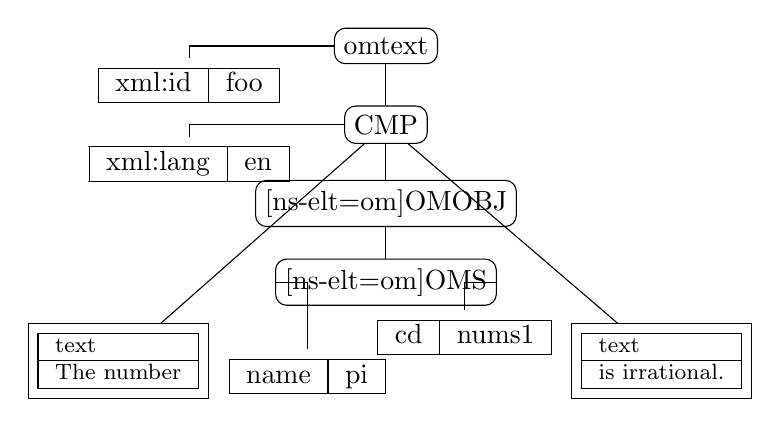
\begin{tikzpicture}
  \node (omtext) [draw,rounded corners] at (2,4) {\element{omtext}};
  \node (CMP) [draw,rounded corners] at (2,3) {\element{CMP}};
  \node (xmlid) at (-.5,3.5) {\begin{tabular}{|c|c|}\hline xml:id& foo \\\hline\end{tabular}};
  \node (xmllang) at (-.5,2.5) {\begin{tabular}{|c|c|}\hline xml:lang& en \\\hline\end{tabular}};
  \node (text1) [draw] at (-1.4,0) {\footnotesize\begin{tabular}{|l|}\hline text\\\hline The number\\\hline\end{tabular}};
  \node (text2) [draw] at (5.5,0) {\footnotesize\begin{tabular}{|l|}\hline text\\\hline is irrational.\\\hline\end{tabular}};
  \node (omobj) [draw,rounded corners] at (2,2) {\element[ns-elt=om]{OMOBJ}};
  \node (oms) [draw,rounded corners] at (2,1)   {\element[ns-elt=om]{OMS}};
  \node (cd) at (3,.3) {\begin{tabular}{|c|c|}\hline cd & nums1 \\\hline\end{tabular}};
  \node (name) at (1,-.2) {\begin{tabular}{|c|c|}\hline name & pi \\\hline\end{tabular}};
  \draw (omtext) -- (CMP);
  \draw (omtext) -| (xmlid);
  \draw (CMP) -- (omobj);
  \draw (CMP) -- (text1);
  \draw (CMP) -- (text2);
  \draw (CMP) -| (xmllang);
  \draw (omobj) -- (oms);
  \draw (oms) -| (cd);
  \draw (oms) -| (name);
\end{tikzpicture}
\end{minipage}
\end{center}
\end{myfig}

Conceptually speaking, {\xml} views a document as a tree\twin{document}{tree} whose nodes
consist of {\indextoo{element}s}, attributes, text nodes, namespace declarations, {\xml}
comments, etc. (see {\myfigref{xml-tree}} for an example\footnote{This tree representation
  glosses over namespace nodes in the tree, but the conceptual tree is sufficient for the
  application in this book.}). For communication this tree is serialized into a
{\atwintoo{balanced}{bracketing}{structure}} (see the listing at the top of
{\myfigref{xml-tree}}), where an element {\snippet{el}} is represented by the brackets
{\snippet{<el>}} (called the {\twindef{opening}{tag}}) and {\snippet{</el>}} (called the
{\twindef{closing}{tag}}). The leaves of the tree are represented by {\twindef{empty}{element}s} (serialized
as {\snippet{<el></el>}}, which can be abbreviated as {\snippet{<el/>}}), and
{\twintoo{text}{node}s} (serialized as a sequence of {\unicode} characters).  An element
node can be annotated by further information using {\twindef{attribute}{node}s} ---
serialized as an {\defin{attribute}} in its opening tag: for instance 
{\snippet{<el visible="no">}} might add the information for a formatting engine to hide this
element. As a document is a tree, the {\xml} specification mandates that there must be a
unique {\twindef{document}{root}}.

Let us now come to a feature that we have glossed over so far: {\xml}
{\defin{namespace}s}~\cite{BraHol:xmlns99}. In many {\xml} applications, we need to mix
several {\xml} vocabularies or languages. In our example in {\myfigref{xml-tree}} we have
three: the {\omdoc} vocabulary with the elements {\element{omtext}} and {\element{CMP}},
the {\openmath} vocabulary with the elements {\element[ns-elt=om]{OMOBJ}} and
{\element[ns-elt=om]{OMS}}, and the general {\xml} vocabulary for the attributes
{\attributeshort[ns-attr=xml]{id}} and {\attributeshort[ns-attr=xml]{lang}}.

To allow a safe mixing of independent {\xml} vocabularies, {\xml} can associate
elements and attributes\footnote{Traditionally most {\xml} applications use attributes
  that are not namespaced.} with a {\defemph{namespace}}\twin{XML}{namespace}, which is
simply a URI that uniquely identifies the intended vocabulary\footnote{Note that it need
  not be a valid {\indextoo{URL}} ({\atwintoo{uniform}{resource}{locator}}; i.e.  a
  pointer to a document provided by a web server).}.  In {\xml} syntax,
{\twintoo{namespace}{membership}} is represented by {\twintoo{namespace}{declaration}s}
and {\twintoo{qualified}{name}s}.

A {\twindef{namespace}{declaration}} is a pseudo-attribute with name {\snippetin{xmlns}}
whose value is a namespace URI {\llquote{nsURI}} (see e.g. the first line in
{\myfigref{xml-tree}}). In a nutshell, a namespace declaration specifies that this element
and all its descendants are in the namespace {\llquote{nsURI}}, unless they have a
namespace declaration of their own or there is a namespace declaration in a closer
ancestor that overwrites it.

Similarly, a {\twindef{namespace}{abbreviation}} can be declared on any element by a
pseudo-attribute of the form
{\snippet{xmlns:}\llquote{nsa}\snippet{="}\llquote{nsUR}\snippet{"}}, where
{\llquote{nsa}} is an {\xml} simple name, and {\llquote{nsURI}} is the namespace URI.  In
the scope of this declaration (in all descendants, where it is not overwritten) we can
specify that an element or attribute is in the namespace {\llquote{nsURI}} by using a
{\twindef{qualified}{name}}: a pair {\llquote{nsa}\snippet{:}\llquote{el}}, where
{\llquote{nsa}} is a namespace abbreviation and {\llquote{el}} is a
{\twintoo{simple}{name}} (i.e. one that does not contain a colon). In
{\myfigref{xml-tree}}, we have a {\twintoo{namespace}{abbreviation}} in the second line,
which is used for the {\openmath} objects in line five. This rule has one exception: the
{\twin{namespace}{abbreviation}} namespace abbreviation {\snippet{xml}} is reserved for
the {{\xml} namespace\twin{XML}{namespace}} and does not have to be declared.

Since {\xml} elements only encode trees, the distribution of {\indextoo{whitespace}}
(including {\indextoo{line-feed}s}) in non-text elements has no meaning in {\xml}, and can
therefore be added and deleted without effecting the semantics.  {\xml} considers anything
between {\snippetin{<\char33--}} and {\snippetin{-->}} in a document as a
comment\twin{XML}{comment}.  They should be used with care, since they are not necessarily
passed on by the {\xml} parser\twin{XML}{parser}, and therefore might not survive
processing by {\xml} applications.

Material that is relevant to the document, but not valid {\xml}, e.g.  binary data or data
that contains angle brackets or elements that are unbalanced or not part of the {\xml}
application can be encoded by embedding it into {\snippet{CDATA}}
{\defemph{sections}\twin{CDATA}{section}}. A {\snippet{CDATA}} section begins with the
string {\snippet{<[CDATA[}} and suspends the {\xml} parser until the string
{\snippet{]]>}} is found. The result of parsing a {\snippet{CDATA}} section is equivalent
to escaping\twin{XML}{escaping} the five {\xml}-specific characters {\snippet{<}},
{\snippet{>}} {\snippet{"}}, {\snippet{'}}, and {\snippet{\&}} to the {\xml}
entities\twin{XML}{entity} {\snippetin{\&lt;}}, {\snippetin{\&gt;}},
{\snippetin{\&quot;}}, {\snippetin{\&apos;}}, and {\snippetin{\&amp;}}.  For instance, we
have the following correspondence between a {\snippet{CDATA}} section and {\xml}-escaped
content:
\begin{lstlisting}[mathescape]
<[CDATA[a<b<sup>3</sup>]]>     $\quad\hat=\qquad$     a&lt;b&lt;sup&gt;3&lt;/sup&gt;
\end{lstlisting}
As a consequence, an {\xml} application is free to choose the form of its output and the
particular form should not be relied upon.
\end{tsubsection}

\begin{tsubsection}[id=xml-validation,short=Validating XML Doucments]{Validating XML Documents}
  {\xml} offers various mechanisms for specifying a subset of trees (or well-bracketed
  {\xml} documents) as admissible in a given {\xml} application: the most commonly used
  ones are {\defin{document type definition}s} ({\defin{DTD}}~\cite{Bray:XML97}), {\xml}
  {\defemph{schemata}}\twin{XML}{schema}~\cite{XML:Schema}, and {\relaxng}
  schemata~\cite{Vlist:rng03}. All of these are {\twintoo{context-free}{grammar}s} for
  trees, that can be used by a {\twindef{validating}{parser}} to reject {\xml} documents
  that do not conform.  Note that DTDs and schemata cannot enforce all constraints that a
  particular {\xml} application may want to impose on documents.  Therefore validation is
  only a necessary condition for {\defin{validity}} with respect to that application.
  Since the {\xml} schema languages can express slightly stronger sets of constraints and
  are namespace-aware, they allow stronger document validation, and usually take
  {\twintoo{normative}{precedence}} over the DTD if present.

  {\Mylstref{xml-dtd}} shows part of an {\omdoc} document. The first line identifies the
  document as an {\xml} document (version 1.0 of the {\xml} specification).  The second
  and third lines constitute the {\twindef{document type}{declaration}} which specifies
  the DTD and the {\twintoo{document}{root}} element. In this case the {\element{omdoc}}
  element starting in line 4 is the root element and will be validated against the DTD
  identified by the {\twindef{public}{Identifier}}\footnote{A string that allows to
    identify an {\xml} resource, it can be mapped to a concrete URI via the {\xml}
    catalog\twin{XML}{catalog}; see {\mysecref{catalog}} for details.} in line two and
  which can be found at the {\indextoo{URI}} in line three. See {\mychapref{validating}}
  for an in-depth discussion of the {\omdoc} DTD and validation.

\begin{lstlisting}[label=lst:xml-dtd,language=XML,morekeywords={omdoc},mathescape,
  caption={The Structure of an {\xml} Document with DTD},
  index={xml,DOCTYPE,omdoc}
  index={[2]xmlns,xmlns:xsi,xsi:schemaLocation}]
<?xml version="1.0"?> 
<!DOCTYPE omdoc PUBLIC "-//OMDoc//DTD OMDoc V1.3//EN"
                       "http://omdoc.org/dtd/omdoc.dtd"> 
<omdoc xml:id="example-omdoc" xmlns="http://omdoc.org/ns"> 
$\ldots$
</omdoc>
\end{lstlisting}
  Note that it is not mandatory to have a {\twintoo{document type}{declaration}} in an
  {\xml} document, or that an {\xml} parser even read it (we call an {\xml} parser
  {\defemph{validating}\atwin{validating}{XML}{parser}} if it does). If no
  {\twintoo{document type}{declaration}} is present, then a parser will just check for
  {\xml}-well-formedness, and possibly rely on some schema for further
  validation\footnote{Note that {\relaxng} schemata do not have a specified in-document
    means for associating a schema with elements. For the way to associate an {\xml}
    schema with a document we refer to {\xml} schema recommendation~\cite{XML:Schema} or
    the {\xml} literature.}.  Note that if a validating parser reads an {\xml} document
  with a {\twintoo{document type}{declaration}}, then it must process it and validate the
  document.

  But a DTD not only contains information for validation, it also
  \begin{description}
  \item[{\bf{declares {\xml} entities\twin{XML}{entity}}}] {\xml} entities are strings of
    the form {\snippet{\&}\llquote{abbr}\snippet{;}}, which abbreviate sequences of
    {\unicode} characters and are expanded by the parser as it reads the document.
  \item[{\bf{supplies default values for attributes}}] which are added to the
    representation of the parsed document by the parser as it reads the document.
  \item[{\bf{declares types of attributes}}] This is is relevant for
    {\twintoo{attribute}{type}s} {\snippetin{ID}} and {\snippetin{IDREF}}. The former are
    required to be {\indextoo{document-unique}} (as well as being {\xml}
    {\twintoo{simple}{name}s~\cite[section 2.3]{Bray:XML97}}) and the latter must point to
    an existing {\snippet{ID}}-type attribute in the same document.
  \end{description}
  {\snippet{ID}}-type attributes are commonly used to identify elements in {\xml}
  documents (see the discussion in {\mysubsecref{xml-fragments}}), which raises a subtle
  point with respect to DTDs. If an {\xml} document is processed without a
  {\twintoo{document type}{declaration}} or by a non-validating parser, the information
  which attributes are {\snippet{ID}}-type ones is lost, and referencing does not work as
  as expected. Fortunately, there is a recent W3C-solution to this problem: Following the
  {\xml} ID recommendation~\cite{XML:id05} {\xml} parsers must recognize attributes of the
  form {\attributeshort[ns-attr=xml]{id}} as {\snippet{ID}}-type attributes, even if no
  DTD is present.

  However DTDs may still serve an important role, even if they are superseded by schema-based
  approaches for pure validation. For instance a format like {\pmathml} (see
  {\mysubsecref{math-markup:mathml}}) seems dependent on a DTD, since it needs to define a
  rich set of mnemonic entities\twin{mnemonic}{entity} for mathematical symbols in
  {\unicode} and uses {\snippet{ID}}-type attributes for cross-referencing. Formats like
  {\cmathml} ({\mysubsecref{math-markup:mathml}}), {\openmath}
  (\mysubsecref{math-markup:openmath}) or {\omdoc} proper can live without DTDs, since they
  do not.
\end{tsubsection}

\begin{tsubsection}[id=xml-fragments]{XML Fragments and URI References}

  As documents are construed as trees in {\xml}, the notion of a document fragment becomes
  definable simply as a sets of well-formed sub-trees. Building on this, URLs and URIs can
  be extended to references of document fragments. These {\twindef{URI}{reference}s} are
  traditionally considered to consist of two parts: A proper URI and a specific
  {\twindef{fragment}{identifier}} separated by the {\twintoo{hash}{character}}
  {\snippet{\#}}. The URI identifies an {\xml} document on the web, whereas the fragment
  identifier identifies a specific fragment of that document.

  {\xml} provides the {\xpointer} framework~\cite{GroMal:xf03} for fragment
  identifiers. It specifies multiple schemes for fragment identifiers. Fragment
  identifiers of the form {\snippet{xpointer(\llquote{path})}} use an
  {\xpath}~\cite{ClaDeR:xpath99} expression {\snippet{\llquote{path}}} to specify a path
  through the document tree leading to the desired element (see~\cite{DeRMal:xxs03}).
  Fragment identifiers in the {\snippet{element()}} scheme~\cite{GroMal:xes03} use
  expressions of the form {\snippet{element(\llquote{cpath})}}, where
  {\snippet{\llquote{cpath}}} is an {\snippet{ID}}-type\twin{type}{ID} identifier together
  with a simple child-path; e.g.  {\snippet{element(foo/3/7)}} identifies the $7^{th}$
  child of the $3^{rd}$ child of the (unique) element that has {\indextoo{ID-type}}
  attribute with value {\snippet{foo}}.

  {\twintoo{URI}{reference}s} of the form {\snippet{\llquote{uri}\#\llquote{id}}} as they
  are used in {\html} to refer to {\twintoo{named}{anchor}s} ({\snippet{<a
      name="\llquote{id}"/>}}) are regained as a special case (the shorthand
  {\snippet{xpointer}}\twin{shorthand}{xpointer}): If {\snippet{\llquote{uri}}} is a URI
  of an {\xml} document $D$ then {\snippet{\llquote{uri}\#\llquote{id}}} refers to the
  unique element in $D$, that has an attribute of type {\snippet{ID}}\twin{type}{ID} with
  value {\snippet{\llquote{id}}}.
\end{tsubsection}

\begin{tsubsection}[id=xml-summary]{Summary}
  In summary, {\xml} provides a widely standardized infrastructure for defining Internet
  markup languages based on tree structures rather than on sequences of characters. {\xml}
  processors like parsers, serializers, {\xml} databases, and {\xslt} transformation
  engines are widely deployed and incorporated into many programming languages. Building
  {\xml} applications on top of this infrastructure frees the implementers from dealing
  with low-level details of parsing, validation, and mass storage. It is no surprise that
  {\xml} has become one of the most successful interoperability formats in information
  technology.

  Note that the use of {\xml} does not give any support for mathematics in itself, since
  the tree models are completely general. It is the role of specific {\xml} applications
  like the ones we will present in the next two chapters to specialize the {\xml} tree
  structures to representations that can be interpreted as mathematical objects and
  documents.
\end{tsubsection}
\end{tsection}
\end{tchapter}
%%% Local Variables: 
%%% mode: latex
%%% TeX-master: "omdoc"
%%% End: 

% LocalWords:  tex sec om br ns xmlns nsa nsURI dtd lst morekeywords xsi xsd lt
% LocalWords:   gt unicode xml Xml DVI pre locator URIs omobj omobj
% LocalWords:  locators CSS eXtensible formulae uri xpointer xpath sdf DOCTYPE
% LocalWords:  namespace CDATA cpath foo mathescape attr nxml tensible arkup cd
% LocalWords:  anguage omtext CMP lang OMOBJ nums xmlid xmllang omobj omobj el
% LocalWords:  omobj elt nsUR apos omdoc IDREF rsp mathml openmath th omobj
% LocalWords:  schemaLocation

%%%%%%%%%%%%%%%%%%%%%%%%%%%%%%%%%%%%%%%%%%%%%%%%%%%%%%%%%%%%%%%%%%%%%%%%%
% This file is part of the LaTeX sources of the OMDoc 1.3 specification
% Copyright (c) 2006 Michael Kohlhase
% This work is licensed by the Creative Commons Share-Alike license
% see http://creativecommons.org/licenses/by-sa/2.5/ for details
\svnInfo $Id: math-markup.tex 9251 2012-07-23 10:29:02Z kohlhase $
\svnKeyword $HeadURL: https://svn.omdoc.org/repos/omdoc/branches/omdoc-1.3/doc/spec/math-markup.tex $
%%%%%%%%%%%%%%%%%%%%%%%%%%%%%%%%%%%%%%%%%%%%%%%%%%%%%%%%%%%%%%%%%%%%%%%%%

\begin{tchapter}[id=math-markup]{Markup for Mathematical Knowledge}

  Mathematicians make use of various kinds of documents (e.g. e-mails, letters,
  pre-prints, journal articles, and textbooks) for communicating mathematical
  knowledge. Such documents employ specialized notational conventions and visual
  representations to convey the mathematical knowledge reliably and efficiently.  The
  respective representations are supported by pertinent   markup systems like
  {\TeX/\LaTeX}.

  Even though mathematical documents can vary greatly in their level of presentation,
  formality and rigor, there is a level of deep semantic structure that is common to all
  forms of mathematics and that must be represented to capture the essence of the
  knowledge. As John R. Pierce has written in his book on communication
  theory~\cite{Pierce:aitit80}, mathematics and its notations should not be viewed as one
  and the same thing. Mathematical ideas exist independently of the notations that
  represent them. However, the relation between meaning and notation is subtle, and part
  of the power of mathematics to describe and analyze derives from its ability to
  represent and manipulate ideas in symbolic form. The challenge in putting mathematics on
  the {\twintoo{World Wide}{Web}} is to capture both notation and content (that is,
  meaning) in such a way that documents can utilize the highly-evolved notational forms of
  written and printed mathematics, and the potential for interconnectivity in electronic
  media.

  In this chapter, we present the state of the art for representing mathematical documents
  on the web and analyze what is missing to mark up mathematical knowledge.  We posit that
  there are three levels of information in mathematical knowledge: formulae, mathematical
  statements, and the large-scale theory structure (constructing the context of
  mathematical knowledge). The first two are immediately visible in marked up mathematics,
  e.g.  textbooks, the third is largely left to an implicit meta-level of mathematical
  communication, or the organization of mathematical libraries. We will discuss these
  three levels in the next sections.

\begin{tsection}[id=math-objects]{Mathematical Objects and Formulae}

  A distinguishing feature of mathematical documents is the use of a complex and highly
  evolved system of two-dimensional symbolic notations, commonly called (mathematical)
  {\defemph{formulae}}\twin{mathematical}{formula}. Formulae serve as representations of
  {\twintoo{mathematical}{object}s}, such as {\indextoo{function}s},
  {\indextoo{group}s}, or {\twintoo{differential}{equation}s}, and
  also of statements about them, like the ``{\twintoo{Fundamental Theorem of}{Algebra}}''.

  The two best-known open markup formats for representing mathematical formulae for the
  Web are {\mathml}~\cite{CarIon:MathML03} and {\openmath}~\cite{BusCapCar:2oms04}. There
  are various other formats that are proprietary or based on specific mathematical
  software packages like {\indextoo{Wolfram Research}}'s {\mathematica}~\cite{Wolfram.02}.
  We will not concern ourselves with them, since we are only interested in open formats.
  Furthermore, we will only give a general overview for the open formats here to survey
  the state of the art, since content {\mathml} and {\openmath} are used for formula
  representation in the {\omdoc} format and thus the technical details of the two markup
  schemes are covered in more detail in the {\omdoc} specification in {\mychapref{mobj}}.
  {\myfigref{math-markup-formulae}} gives an overview over the current state of the
  standardization activities.

    \begin{myfig}{math-markup-formulae}{The Status of Markup Standardization for
        Mathematical Formulae}
      \begin{tabular}{|l|p{4cm}|p{4.4cm}|}\hline
        language & {\mathml}           & {\openmath}\\\hline\hline
        by       & W3C Math WG         & {\openmath} society\\\hline
        origin   & math for {\html}    & integration of CAS \\\hline
        coverage & content + presentation; K-14     & content; extensible \\\hline
        status   & Version 2.2e ({\rm VI} 2003) & Version 2 ({\rm VI} 2004) \\\hline
        activity & maintenance         & maintenance \\\hline
        Info     & {\small\url{http://w3c.org/Math/}} & 
                   {\small\url{http://www.openmath.org/}}    \\\hline
      \end{tabular}
    \end{myfig}

    {\openmath} was originally a development driven mainly by the Computer Algebra
    community in Europe trying to standardize the communication of mathematical objects
    between Computer Algebra Systems. The format has been discussed in a series of
    workshops and has been funded by a series of grants by the European Union. This
    process led to the {\openmath} 1 standard in June 1999 and eventually to the
    incorporation of the {\openmath} society as the institutional guardian of the
    {\openmath} standard. {\mathml} has developed out of the effort to include
    presentation primitives for mathematical notation (in {\TeX}{\index{tex@\TeX}}
    quality) into {\html}, and was the first {\xml} application\twin{XML}{application} to
    reach {\indextoo{recommendation}} status\footnote{As such, {\mathml} played a great
      role as technology driver in the development of {\xml}. This role gives {\mathml} a
      somewhat peculiar status at the W3C; it is the only ``vertical''
      (application/domain-driven) {\xml} application standardized by the W3C, which
      otherwise concentrates on ``horizontal'' (technology-driven) standards.} at the
    {\indextoo{W3C}}~\cite{IonMin:MathML99}.
    
    The competition and collaboration between these two approaches to representation of
    mathematical formulae and objects has led to a large overlap between the two developer
    communities.  {\mathml} deals principally with the {\emph{presentation}} of
    mathematical objects, while {\openmath} is solely concerned with their semantic
    meaning or {\emph{content}}.  While {\mathml} does have some limited facilities for
    dealing with content, it also allows semantic information encoded in {\openmath} to be
    embedded inside a {\mathml} structure.  Thus the two technologies may be seen as
    highly compatible\footnote{e.g. {\mathml} is the preferred presentation format for
      {\openmath} objects and {\openmath} content dictionaries are the primary
      specification language for {\mathml} semantics.} and complementary (in aim).

\begin{tsubsection}[id=math-markup:mathml]{{\mathml}}
  \begin{center}
    \fbox{\begin{minipage}{9cm} {\mathml} is an {\xml} application for describing
        mathematical {\emph{notation}} and capturing both its {\emph{structure}} and
        {\emph{content}}. The goal of {\mathml} is to enable mathematics to be served,
        received, and processed on the World Wide Web, just as {\html} has enabled this
        functionality for text.\\\strut\hfill{\emph{from the MathML2
            Recommendation}~\cite{CarIon:MathML03}}
     \end{minipage}}
 \end{center}

 To reach this goal, {\mathml} offers two sub-languages: {\pmathml} for marking up the
 two-dimensional, visual appearance of mathematical formulae, and {\cmathml} as a markup
 infrastructure for the functional structure of mathematical formulae.

 To mark up the visual appearance of formulae {\pmathml} represents mathematical formulae
 as a tree of layout primitives. For instance the expression $3\over x+2$ would be
 represented as the layout tree in {\myfigref{pmathml-tree}}. The layout primitives
 arrange ``inner boxes'' (given in black) and provide an outer box (given in gray here)
 for the next level of layout. In {\myfigref{pmathml-tree}} we see the general layout
 schemata for numbers ({\element[ns-elt=m]{mn}}), identifiers ({\element[ns-elt=m]{mi}}),
 operators ({\element[ns-elt=m]{mo}}), bracketed groups ({\element[ns-elt=m]{mfence}}),
 and fractions ({\element[ns-elt=m]{mfrac}}); others include horizontal grouping
 ({\element[ns-elt=m]{mrow}}), roots ({\element[ns-elt=m]{mroot}}), scripts
 ({\element[ns-elt=m]{msup}}, {\element[ns-elt=m]{msub}}, {\element[ns-elt=m]{msubsup}}),
 bars and arrows ({\element[ns-elt=m]{munder}}, {\element[ns-elt=m]{mover}},
 {\element[ns-elt=m]{munderover}}), and scoped {\css} styling
 ({\element[ns-elt=m]{mstyle}}). Mathematical symbols are taken from {\unicode} and
 provided with special mnemonic entities by the {\mathml} DTD, e.g. {\snippet{\&sum;}} for
 $\Sigma$.

    \begin{myfig}{pmathml-tree}{The Layout Tree for the Formula $3\over x+2$}
\begin{minipage}{2.4cm}
\begin{lstlisting}[numbers=none,frame=none]
<m:mfrac>
 <m:mn>3</m:mn>
 <m:mfenced>
   <m:mi>x</m:mi>
   <m:mo>+</m:mo>
   <m:mn>2</m:mn>
 </m:mfenced>
</m:mfrac>
\end{lstlisting}
\end{minipage}\hspace{2em}
      \begin{minipage}{8cm}
  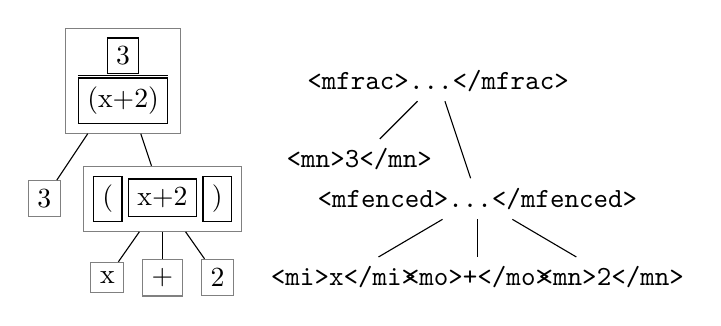
\begin{tikzpicture}
    \node[draw=gray] (frac)  at (2.5,4) {$\fbox{3}\over\fbox{(x+2)}$};
    \node[draw=gray] (3) at (1.5,2.5) {3};
    \node[draw=gray] (fence) at (3,2.5) {\fbox{(}\kern2pt\fbox{x+2}\kern2pt\fbox{)}};
    \node[draw=gray] (x) at (2.3,1.5){x};
    \node[draw=gray] (+) at (3,1.5) {+};
    \node[draw=gray] (2) at (3.7,1.5) {2};
    \draw (frac) -- (3);
    \draw (frac) -- (fence);
    \draw (fence) -- (x);
    \draw (fence) -- (+);
    \draw (fence) -- (2);

    \node (mfrac) at (6.5,4) {\tt{<mfrac>\ldots</mfrac>}};
    \node (m3) at (5.5,3) {{\tt{<mn>3</mn>}}};
    \node (mfence) at (7,2.5) {{\tt{<mfenced>\ldots</mfenced>}}};
    \node (mx) at (5.3,1.5) {{\tt{<mi>x</mi>}}};
    \node (m+) at (7,1.5) {{\tt{<mo>+</mo>}}};
    \node (m2) at (8.7,1.5)  {{\tt{<mn>2</mn>}}};
    \draw (mfrac) -- (m3);
    \draw (mfrac) -- (mfence);
    \draw (mfence) -- (mx);
    \draw (mfence) -- (m+);
    \draw (mfence) -- (m2);
  \end{tikzpicture}
\end{minipage}  
\end{myfig}

Since the aim of {\mathml} is to do most of the formatting inside the browser, where
resource considerations play a large role, it restricts itself to a fixed set of
mathematical concepts -- the {\indextoo{K-14}} fragment ({\indextoo{Kindergarten}} to
$14^{th}$ grade; i.e. undergraduate college level) of mathematics. K-14 contains a large
set of commonly used glyphs for mathematical symbols and very general and powerful
presentation primitives, similar to those that make up the lower level of {\TeX}.
However, it does not offer the programming language features of {\TeX}\footnote{{\TeX}
  contains a full, {\indextoo{Turing}}-complete -- if somewhat awkward -- programming
  language that is mainly used to write {\twintoo{style}{file}}s.  This is separated out
  by {\mathml} to the {\css} and {\xslt} style languages it inherits from {\xml}.}  for
the obvious computing resource considerations.  {\pmathml} is supported by current
versions of the browsers {\amaya}~\cite{amaya_web}, {\msie}~\cite{ie_web} (via the
{\mathplayer} plug-in~\cite{mathplayer_web}), and {\mozilla}~\cite{mozilla_web}.

  {\mathml} also offers content markup for mathematical formulae, a sub-language called
  {\defemph{{\cmathml}}} to contrast it from the {\defemph{{\pmathml}}} described
  above. Here, a mathematical formula is represented as a tree as well, but instead of
  marking up the visual appearance, we mark up the functional structure. For our example
  $3\over x+2$ we obtain the tree in {\myfigref{cmathml-tree}}, where we use @ as the
  function application operator (it interprets the first child as a function and applies
  it to the rest of the children as arguments).

\begin{myfig}{cmathml-tree}{The functional Structure of $3\over x+2$}
\begin{minipage}{3cm}
\begin{lstlisting}[numbers=none,frame=none]
<m:apply>
  <m:divides/>
  <m:cn>3</m:cn>
  <m:apply>
    <m:plus/>
    <m:ci>x</m:ci>
    <m:cn>2</m:cn>
  </m:apply>
</m:apply>
\end{lstlisting}
\end{minipage}\hspace*{3em}
\begin{minipage}{4cm}
  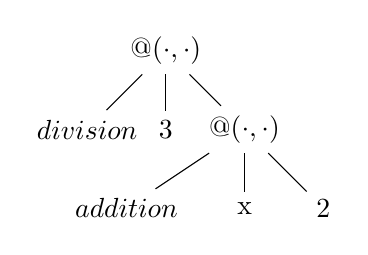
\begin{tikzpicture}
    \node (app1)  at (2.5,3.5) {$\hbox{@}(\cdot,\cdot)$};
    \node (div) at (1.5,2.5) {$division$};
    \node (3) at (2.5,2.5) {3};
    \node (app2) at (3.5,2.5) {$\hbox{@}(\cdot,\cdot)$};
    \node (plus) at (2,1.5){$addition$};
    \node (x) at (3.5,1.5) {x};
    \node (2) at (4.5,1.5) {2};
    \draw (app1) -- (div);
    \draw (app1) -- (3);
    \draw (app1) -- (app2);
    \draw (app2) -- (plus);
    \draw (app2) -- (x);
    \draw (app2) -- (2);
  \end{tikzpicture}
\end{minipage}
\end{myfig}

{\cmathml} offers around 80 specialized elements for the most common K-14 functions and
individuals. In {\myfigref{cmathml-tree}} we see function application
({\element[ns-elt=m]{apply}}), content identifiers ({\element[ns-elt=m]{ci}}), content
numbers ({\element[ns-elt=m]{cn}}) and the functions for division
({\element[ns-elt=m]{divide}}) and addition ({\element[ns-elt=m]{plus}}).

Finally, {\mathml} offers a specialized {\element[ns-elt=m]{semantics}} element that
allows to annotate {\mathml} formulae with alternative representations. This feature can
be used to provide combined content- and presentation-{\mathml} representations.
{\Myfigref{pcmml}} shows an example of this for our expression $3\over x+2$. The outermost
{\element[ns-elt=m]{semantics}} element is used for mixing presentation and content
markup. The first child of the {\element[ns-elt=m]{semantics}} element contains {\pmathml}
(this is used by the {\mathml}-aware browser), the subsequent
{\element[ns-elt=m]{annotation-xml}} element contains {\cmathml} markup for the same
formula. Corresponding sub-expressions are {\indextoo{co-reference}d} by
{\indextoo{cross-reference}s}: The presentation element carries an
{\attributeshortcomment{id}{in {\sc{MathML}}}} attribute, which serves as the target for
an {\attribute[ns-attr=xlink]{href}{in {\sc{MathML}}}} attribute in the content
markup. This technique is called {\twintoo{parallel}{markup}}, it allows to select logical
sub-expressions by selecting layout sub-schemata\twin{layout}{schema} in the browser,
e.g. for copy and paste. Note that a {\element[ns-elt=m]{semantics}} element can have more
than one {\element[ns-elt=m]{annotation-xml}} child, so that other content formats such as
{\openmath} can also be incorporated.

\begin{myfig}{pcmml}{Mixing Presentation and {\cmathml}}
  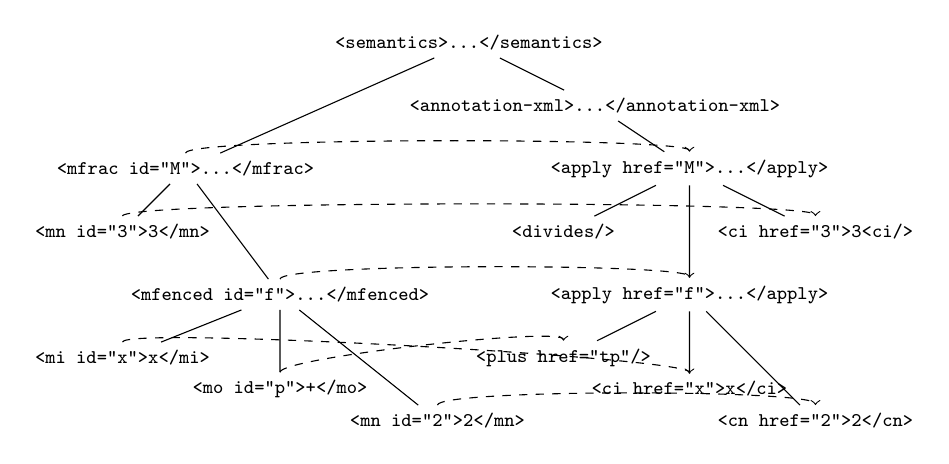
\begin{tikzpicture}[scale=.8]\scriptsize
    \tikzstyle{every node}=[font=\ttfamily]
    \node (semantics) at (6,6) {<semantics>\ldots</semantics>};
    \node (ann) at (8,5) {<annotation-xml>\ldots</annotation-xml>};
    \node (mfrac) at (1.5,4) {<mfrac id="M">\ldots</mfrac>};
    \node (m3) at (0.5,3)    {<mn id="3">3</mn>};
    \node (mfence) at (3,2) {<mfenced id="f">\ldots</mfenced>};
    \node (mx) at (0.5,1)  {<mi id="x">x</mi>};
    \node (m+) at (3,.5)     {<mo id="p">+</mo>};
    \node (m2) at (5.5,0)   {<mn id="2">2</mn>};
    \node (apply) at (9.5,4){<apply href="M">\ldots</apply>};
    \node (div) at (7.5,3)  {<divides/>};
    \node (c3) at (11.5,3)  {<ci href="3">3<ci/>};
    \node (apply2) at (9.5,2) {<apply href="f">\ldots</apply>};
    \node (plus) at (7.5,1) {<plus href="tp"/>};
    \node (cx) at (9.5,.5)  {<ci href="x">x</ci>};
    \node (c2) at (11.5,0)  {<cn href="2">2</cn>};

    \draw (semantics) -- (ann);
    \draw (semantics) -- (mfrac);
    \draw (mfrac) -- (m3);
    \draw (mfrac) -- (mfence);
    \draw (mfence) -- (mx);
    \draw (mfence) -- (m+);
    \draw (mfence) -- (m2);
    \draw (ann) -- (apply);
    \draw (apply) -- (div);
    \draw (apply) -- (apply2);
    \draw (apply) -- (c3);
    \draw (apply2) -- (plus);
    \draw (apply2) -- (cx);
    \draw (apply2) -- (c2);
    
    \draw[->,dashed] (mfrac) .. controls +(up:.5cm) and +(up:.5cm)  .. (apply);
    \draw[->,dashed] (m3) .. controls +(up:.5cm) and +(up:.5cm)  .. (c3);
    \draw[->,dashed] (mfence) .. controls +(up:.5cm) and +(up:.5cm)  .. (apply2);
    \draw[->,dashed] (m+) .. controls +(up:.5cm) and +(up:.5cm)  .. (plus);
    \draw[->,dashed] (mx) .. controls +(up:.5cm) and +(up:.5cm)  .. (cx);
    \draw[->,dashed] (m2) .. controls +(up:.5cm) and +(up:.5cm)  .. (c2);
  \end{tikzpicture}
\end{myfig}
\end{tsubsection}

\begin{tsubsection}[id=math-markup:openmath]{\openmath}
  \begin{center}
    \fbox{\begin{minipage}{9cm} [\ldots]
        {\openmath}: a standard for the representation and
        communication of mathematical objects. [\ldots]\\
        {\openmath} allows the {\emph{meaning}} of an object to be encoded rather than
        just a visual representation.  It is designed to allow the free exchange of
        mathematical objects between software systems and human beings.  On the worldwide
        web it is designed to allow mathematical expressions embedded in web pages to be
        manipulated and computed with in a meaningful and correct way.  It is designed to
        be machine-generatable and machine-readable, rather than written by
        hand.\\\strut\hfill{\emph{from the {\openmath}2 Standard}~\cite{BusCapCar:2oms04}}
      \end{minipage}}
  \end{center}

  Driven by the intention of representing the {\emph{meaning}} of mathematical objects
  expressed in the quote above, the {\openmath} format is not primarily an {\xml}
  application. Rather, {\openmath} defines an abstract (mathematical) object model for
  mathematical objects and specifies an {\xml} encoding (and a binary\footnote{The binary
    encoding allows to optimize encoding size and (more importantly) parsing time for
    large {\openmath} objects. The binary encoding for {\openmath} objects will not play a
    role for the {\omdoc} format, so we will not pursue this here.}  encoding) for
  that\footnote{The {\mathml} specification is very vague on what the meaning of
    {\cmathml} fragments might be; we have to assume that its {\xml} {\twintoo{document
        object}{model}}~\cite{URL:DOM} or the or its
    {\indextoo{infoset}}~\cite{CowTob:xis04} must be.}.

  The central construct of {\openmath} is that of an {\defemph{{\openmath}
      object}}\index{object!{\sc OpenMath}}\index{OpenMath@{\sc OpenMath}! object}
  (realized by the element {\element[ns-elt=om]{OMOBJ}} in the {\xml} encoding), which has
  a tree-like representation made up of {\indextoo{application}s}
  ({\element[ns-elt=om]{OMA}}), {\indextoo{binding structure}s}
  ({\element[ns-elt=om]{OMBIND}} using {\element[ns-elt=om]{OMBVAR}} to specify the
  {\twintoo{bound}{variable}s}\footnote{Binding structures are somewhat awkwardly realized
    via the {\element[ns-elt=m]{apply}} element with an {\element[ns-elt=m]{bvar}} child
    in {\cmathml}.}), {\indextoo{variable}s} ({\element[ns-elt=om]{OMV}}), and
  {\indextoo{symbol}s} ({\element[ns-elt=om]{OMS}}). 

  The handling of symbols --- which are used to represent the multitude of mathematical
  domain constants --- is maybe the largest difference between {\openmath} and {\cmathml}.
  Instead of providing elements for all K-14 concepts, the {\openmath} standard adds an
  extension mechanism for mathematical concepts, the {\defemph{content
      dictionaries}}\twin{content}{dictionary}.  These are {\indextoo{machine-readable}}
  documents that define the meaning of mathematical concepts expressed by {\openmath}
  symbols.  Just like the library mechanism of the {\atwintoo{C}{programming}{language}},
  they allow {\openmath} to externalize the definition of extended language concepts. As a
  consequence, {\indextoo{K-14}} need not be part of the {\openmath} language, but can be
  defined in a set of content dictionaries (see~\cite{URL:omcd-core}).

  The {\element[ns-elt=om]{OMS}} element carries the attributes {\attribute{cd}{OMS}} and
  {\attribute{name}{OMS}}.  The {\attribute{name}{OMS}} attribute gives the name of the
  symbol, the {\attribute{cd}{OMS}} attribute specifies the {\indextoo{content
      dictionary}}. As variables do not carry a meaning independent of their local
  content, {\element[ns-elt=om]{OMV}} only carries a {\attribute{name}{OMV}}
  attribute. See {\mylstref{om-comm}} for an example that uses most of the elements.

\begin{lstlisting}[label=lst:om-comm,
    caption={{\openmath} Representation of $\allcdot{a,b}{a+b=b+a}$},
    language=OpenMath,
    index={OMOBJ,OMBIND,OMS,OMBVAR,OMV,OMATTR,OMATP}]
<OMOBJ xmlns="http://www.openmath.org/OpenMath">                            
  <OMBIND cdbase="http://www.openmath.org/cd">                          
    <OMS cd="quant1" name="forall"/> 
    <OMBVAR><OMV name="a"/><OMV name="b"/></OMBVAR>                        
    <OMA><OMS cd="relation" name="eq"/> 
      <OMA><OMS cd="arith1" name="plus"/>
        <OMV name="a"/>               
        <OMV name="b"/>               
      </OMA>                         
      <OMA><OMS cd="arith1" name="plus"/>
        <OMV name="b"/>               
        <OMV name="a"/>               
      </OMA>      
    </OMA>                           
  </OMBIND>                         
</OMOBJ>
\end{lstlisting}
  {\Mylstref{om-comm}} shows the {\xml} encoding of the law of commutativity for addition
  (the formula $\allcdot{a,b}{a+b=b+a}$) in {\openmath}. Note that as we have discussed
  above, this representation is not self-contained but relies on the availability of
  content dictionaries\index{content dictionary} {\snippet{quant1}},
  {\snippet{relation1}}, and {\snippet{arith1}}. Note that in this example they can be
  accessed via the URL specified in the {\attribute[ns-elt=om]{cdbase}{OMOBJ}} attribute,
  but in general, the content dictionaries are only used for {\emph{identification of
      symbol}s}. In particular, in the classical {\openmath} model, content dictionaries
  are only viewed as a resource for system developers, who use them as a reference decide
  which symbol to use in an export/import facility for a {\twintoo{computer
      algebra}{system}}. In the communication between mathematical software systems, they
  are no longer needed: If two systems agree on a set of content dictionaries, then they
  agree on the meaning of all {\openmath} objects that can be constructed using their
  symbols (the meaning of applications and bindings is known from the folklore).

  The content dictionary architecture is the greatest strength of the {\openmath}
  format. It establishes an object model and {\xml} encoding based on what we call
  ``\twintoo{semantics}{by pointing}''. Two {\openmath} objects have the same meaning in
  this model, iff they have the same structure and all symbols point to the same content
  dictionaries\footnote{Note that we can interpret the {\cmathml} model as a ``semantics
    by pointing'' model as well. Only that here the K-14 elements do not point to
    machine-readable content dictionaries, but at the (human-readable) {\mathml}
    specification, which specifies their meaning.}.

  In the standard encoding of {\openmath} content dictionary, the meaning of a symbol is
  specified by a set of
  \begin{description}
  \item[{\bf{``formal mathematical properties\atwin{formal}{mathematical}{property}''}}]
    The {\element[ns-elt=omcd]{FMP}} element contains an {\openmath} object that expresses
    the desired property.
  \item[{\bf{``commented mathematical
        properties\atwin{commented}{mathematical}{property}''}}] The
    {\element[ns-elt=omcd]{CMP}} element contains a natural language description of a
    desired property.
  \end{description}
  For instance, the specification in {\mylstref{arith1}} is part of the standard
  {\openmath} content dictionary {\snippetin{arith1.ocd}}~\cite{URL:omcd-core} for the
  elementary arithmetic operations.\footnote{The content of the
    {\element[ns-elt=omcd]{FMP}} element is actually the {\openmath} object in the
    representation in {\mylstref{om-comm}}, we have abbreviated it here in the usual
    mathematical notation, and we will keep doing this in the remaining document: wherever
    an {\xml} element in a figure contains mathematical notation, it stands for the
    corresponding {\openmath} element.}
\begin{lstlisting}[label=lst:arith1,language=omCD,mathescape,
  caption={Part of the {\sc OpenMath} Content Dictionary {\snippet{arith1}}.},
  index={CDDefinition,Name,dc:description,CMP,FMP}]
<CDDefinition>
  <Name>plus</Name> 
  <CDDescription>
    The symbol representing an n-ary commutative function plus.
  </CDDescription> 
  <CMP><xhtml:p>for all a,b | a + b = b + a</xhtml:p></CMP>
  <FMP>$\allcdot{a,b}{a+b=b+a}$</FMP> 
</CDDefinition>
\end{lstlisting}

  On the other hand, the content dictionary encoding defined in the {\openmath} standard
  (and the particular content dictionaries blessed by the {\openmath} society) are the
  greatest weakness of {\openmath}.  The represent the knowledge in a very unstructured
  way --- to name just a few problems:
  \begin{itemize}
  \item in the {\element[ns-elt=omcd]{CMP}}, we can only make use of ASCII representation
    of formulae.
  \item The relation between a particular {\element[ns-elt=omcd]{CMP}} and
    {\element[ns-elt=omcd]{FMP}} elements is unclear.
  \item For properties like the {\indextoo{distributivity}} of addition over
    multiplication it is unclear, whether we should express this in the definition of the
    symbol {\snippet{plus}} or the symbol {\snippet{times}}.
  \item Are all properties constitutive{\twin{constitutive}{property}} for the meaning of
    the symbol? Should they be verified for an implementation of a content dictionary?
  \item What is the relationship between content dictionaries? Are they
    {\indextoo{translation-equivalent}}?  Does one entail the other?
  \end{itemize}
  The {\openmath}2 standards acknowledges these problems and explicitly opens up the
  content dictionary format allowing other representations that meet certain minimal
  criteria relegating the standard encoding above to a reference implementation of the
  minimal model.

  We will analyze the questions raised above from a general standpoint when discussing the
  remaining two levels of mathematical knowledge. This analysis constitutes the basic
  intuitions for the {\omdoc} format.
\end{tsubsection}
\end{tsection}

\begin{tsection}[id=meta-math]{Mathematical Texts and Statements}

  The mathematical markup languages {\openmath} and {\mathml} we have discussed in the
  last section have dealt with mathematical objects and formulae. The formats either
  specify the semantics of the mathematical object involved in the standards document
  itself ({\mathml}) or in a fixed set of generally agreed-upon documents ({\openmath}
  content dictionaries\index{content dictionary}). In both cases, the mathematical
  knowledge involved is relatively fixed. Even in the case of {\openmath}, which has an
  extensible library mechanism, the content dictionaries are not in themselves objects of
  communication (they are mainly background reference for the implementation of
  {\openmath} interfaces).

  For the communication among mathematicians (rather than computation systems) this level
  of support is insufficient, because the mathematical knowledge expressed in definitions,
  theorems (stating properties of defined objects), their proofs, and even whole
  mathematical theories is the primary focus of mathematical communication. For content
  markup of mathematical knowledge, we have to turn implicit or presentational structuring
  devices in mathematical documents\twin{document}{mathematical} into explicit ones. For
  instance, {\twindef{mathematical}{statement}s} like the ones in the document fragment in
  {\myfigref{fragment}} are delimited by keywords (e.g. {\bf{Definition}}, {\bf{Lemma}}
  and {\boexchen}) or by changes in text font.

\begin{myfig}{fragment}{A Fragment of a Traditional Mathematical Document}
  \fbox{\begin{minipage}{10cm}
      {\bf Definition 3.2.5} (Monoid)\\
    A monoid is a semigroup $S=(G,\circ)$ with an element $e\in G$, 
    such that $e\circ x=x$ for all $x\in G$. $e$ is called a left 
    unit of $S$.\\[1ex]
    
    {\bf Lemma 3.2.6}\\
    {\emph{A monoid has at most one left unit.}}\\
    {\bf Proof}: We assume that there is another left unit $f$ \ldots\\
    This contradicts our assumption, so we have proven the claim.\hfill\kasten
  \end{minipage}}
\end{myfig}
Of course, the content of a mathematical statement, e.g. the statement of an assertion
that ``addition is commutative'' can be expressed by a {\cmathml} or {\openmath} formula
like the one in {\mylstref{om-comm}}, but the information that this formula is a theorem
that has a proof, cannot be directly expressed without extending the formalism. Even
formalizations of mathematics like Russell and Whitehead's famous ``Principia
Mathematica''~\cite{WhiRus:pm10} treat this information on the meta-level. If we are
willing to extend the mathematical formalism to include primitives for such information,
we arrive at formalisms called {\twindef{logical}{framework}s} (see~\cite{Pfenning:lf01}
for an overview), where they are treated as the primary objects of study. The most
prevalent approach here uses the ``{\twintoo{formulae as}{types}}'' idea that delegates
{\twintoo{mathematical}{formula}e} to the status of types. Logical frameworks capture
{\twintoo{mathematical}{statement}s} in formulae and as such can be expressed in
{\cmathml} or {\openmath}.  However, this approach relies on full formalization of the
mathematical content, and cannot be directly used to capture mathematical practice. In
particular, the gap between formal mathematics and informal (but rigorous) treatments of
mathematics that rely on natural language as we find them in textbooks and journal
articles is wide.  The formalization process is so tedious, that it is seldom executed in
practice (the ``Principia Mathematica'' and the {\mizar} mathematical
library~\cite{MizarKB} are solitary examples).
\end{tsection}

\begin{tsection}[id=meta-theories]{Large-Scale Structure and Context in Mathematics}

  The large-scale structure of mathematical knowledge is much less apparent than that for
  formulae and even statements. Experienced mathematicians are nonetheless aware of it,
  and use it for navigating the vast space of mathematical knowledge and to anchor their
  communication. 

  Much of this structure can be found in networks of {\defemph{ mathematical
      theories}\twin{mathematical}{theory}}: groups of mathematical statements, e.g. those
  in a \indextoo{monograph} ``Introduction to Group Theory'' or a {\indextoo{chapter}} or
  {\indextoo{section}} in a {\indextoo{textbook}}. The relations among such theories are
  described in the text, sometimes supported by mathematical statements called
  {\twintoo{representation}{theorem}s}. We can observe that mathematical texts can only be
  understood with respect to a particular mathematical context given by a theory which the
  reader can usually infer from the document. The context can be stated explicitly
  (e.g. by the title of a book) or implicitly (e.g. by the fact that the e-mail comes from
  a person that we know works on finite groups, and that she is talking about math).

  If we make the structure of the context as explicit as the structure of the mathematical
  objects (we will speak of {\twindef{context}{markup}}), then mathematical software
  systems will be able to provide novel services that rely on this structure. We contend
  that without an explicit representation of context structure, tasks like semantics-based
  searching and navigation or object classification can only be performed by human
  mathematicians that can understand the implicitly given structure.

Mathematical theories {\twin{mathematical}{theory}} have been studied by mathematicians
and logicians in the search of a rigorous foundation for mathematical practice. They have
been formalized as collections of {\twintoo{symbol}{declaration}s} --- giving names to
mathematical objects that are particular to the theory --- and logical formulae, which
state the laws governing the properties of the theory. A key research question was to
determine conditions for the consistency of mathematical theories. In inconsistent
theories all statements are vacuously valid\footnote{A statement is valid in a theory, iff
  it is true for all models of the theory. If there are none, it is vacuously valid.}, and
therefore only consistent theories make interesting statements about mathematical objects.

It is one of the critical observations of meta-mathematics that theories can be extended
without endangering consistency, if the added formulae can be proven from the formulae
already in the theory (such formulae are called {\indextoo{theorem}s}). As a consequence,
consistency of a theory can be determined by examining the {\defin{axiom}s} (formulae
without a proof) alone. Thus the role of proofs is twofold, they allow to push back the
assumptions about the world to simpler and simpler axioms, and they allow to test the
model by deriving consequences of these basic assumptions that can be tested against the
data.
  
  A second important observation is that new symbols together with axioms defining their
  properties can be added to a theory without endangering consistency, if they are of a
  certain restricted syntactical form. These {\twindef{definitional}{form}s} mirror the
  various types of mathematical {\defin{definition}s} (e.g. equational, recursive,
  implicit definitions).  This leads to the ``{\emph{\atwintoo{principle
        of}{conservative}{extension}}}'', which states that conservative extensions to
  theories (by {\indextoo{theorem}s} and {\indextoo{definition}s}) are safe for
  mathematical theories, and that possible sources for inconsistencies\index{inconsistent}
  can be narrowed down to small sets of axioms.

  Even though all of this has theoretically been known to (meta)-mathema\-ticians for
  almost a century, it has only been an explicit object of formal study and exploited by
  mathematical software systems in the last decades. Much of the meta-mathematics has been
  formally studied in the context of proof development systems like
  {\automath}~\cite{Bruijn80} {\nuprl}~\cite{Constable86}, {\hol}~\cite{GoMe93},
  {\mizar}~\cite{Rudnicki:aomp92} and {\OMEGA}~\cite{BenzmuellerEtAl:otama97} which
  utilize strong logical systems that allow to express both mathematical statements and
  proofs as mathematical objects.  Some systems like {\isabelle}~\cite{Paulson90} and
  {\scsys{Twelf}}~\cite{Pfenning91} even allow the specification of the logic language
  itself, in which the reasoning takes place.  Such semi-automated theorem proving systems
  have been used to formalize substantial parts of mathematics and mechanically verify
  many theorems in the respective areas. These systems usually come with a library system
  that manages and structures the body of mathematical knowledge formalized in the system
  so far.

  In software engineering, mathematical theories have been studied under the label of
  ``(algebraic) specifications\twin{algebraic}{specification}''. Theories are used to
  specify the behavior of programs and software components. Under the pressure of
  industrial applications, the concept of a theory (specification) has been elaborated
  from a practical point of view to support the structured development of specifications,
  {\twintoo{theory}{reuse}}, and modularization.  Without this additional structure, real
  world specifications become unwieldy and unmanageable in practice. Just as in the case
  of the theorem proving systems, there is a whole zoo of specification languages, most of
  them tied to particular software systems.  They differ in language primitives,
  theoretical expressivity, and the level of tool support.

  Even though there have been standardization efforts, the most recent one being the
  {\casl} standard (Common Algebraic Specification Language; see~\cite{CoFI:2004:CASL-RM}) there have
  been no efforts of developing this into a general markup language for mathematics with
  attention to web communication and standards. The {\omdoc} format attempts to provide a
  content-oriented markup scheme that supports all the aspects and structure of
  mathematical knowledge we have discussed in this section. Before we define the language
  in the next chapter, we will briefly go over the consequences of adopting a markup
  language like {\omdoc} as a standard for web-based mathematics.

\end{tsection}
\end{tchapter}

%%% Local Variables: 
%%% mode: latex
%%% TeX-master: "omdoc"
%%% End: 

% LocalWords:  tex lst pcmml mrow mo mi ci InvisibleTimes xlink href csymbol cd
% LocalWords:  om OMB OMSTR OMF OME OMATP commm quant eq arith ocd omCD mathe
% LocalWords:  mathescape ti cians mathema ticians th externalize underdefined
% LocalWords:  forall FMP CMP CDDefinition ary mathweb mathematicised omdoc nat
% LocalWords:  comm Principia defn rec xmlns AutoMath Twelf mathml xlink href dc
% LocalWords:  openmath CDDescription ns elt attr cdbase mobj WG CAS pmathml mn
% LocalWords:  mfence mfrac mroot msup msub msubsup munder munderover mstyle mx
% LocalWords:  mfenced frac cmathml cn ann tp cx infoset OMOBJ OMA OMBIND bvar
% LocalWords:  OMBVAR OMV OMATTR omcd  omcd omcd omcd omcd omcd omcd omcd omcd

%%%%%%%%%%%%%%%%%%%%%%%%%%%%%%%%%%%%%%%%%%%%%%%%%%%%%%%%%%%%%%%%%%%%%%%%%
% This file is part of the LaTeX sources of the OMDoc 1.3 specification
% Copyright (c) 2006 Michael Kohlhase
% This work is licensed by the Creative Commons Share-Alike license
% see http://creativecommons.org/licenses/by-sa/2.5/ for details
\svnInfo $Id: omdoc-markup.tex 9330 2014-05-03 14:38:25Z kohlhase $
\svnKeyword $HeadURL: https://svn.omdoc.org/repos/omdoc/branches/omdoc-1.3/doc/spec/omdoc-markup.tex $
%%%%%%%%%%%%%%%%%%%%%%%%%%%%%%%%%%%%%%%%%%%%%%%%%%%%%%%%%%%%%%%%%%%%%%%%%

\begin{tchapter}[id=omdoc-markup,short=Open Mathematical Documents]{OMDoc: Open Mathematical Documents}

  Based on the analysis of the structure inherent in mathematical knowledge and existing
  content markup systems for mathematics we will now briefly introduce basic design
  assumptions and the development history of the {\omdoc} format, situate it, and discuss
  possible applications.

  \begin{tsection}[id=omdoc-history]{A Brief History of the {\omdoc} Format}
    {\omdoc} initially developed from the quest for a solution of the problem of
    representing knowledge on the one hand and integrating external mathematical reasoning
    systems in the {\OMEGA} project at Saarland University on the
    other. {\OMEGA}~\cite{SiekmannEtAl:pdwo02} is a large-scale
    {\atwintoo{proof}{development}{environment}} that integrates various reasoning engines
    ({\atwintoo{automated}{theorem}{prover}s}, {\twintoo{decision}{procedure}s},
    {\twintoo{computer algebra}{system}s}) via
    {\atwintoo{knowledge-based}{proof}{planning}} with the aim of creating a
    {\atwintoo{mathematical}{assistant}{system}}.

    \begin{tsubsection}{The Design Problem}
      One of the hard practical problems of building such systems is to represent,
      provision, and manage the relevant (factual\twin{factual}{knowledge}, tactic, and
      intuitive\twin{intuitive}{knowledge}) knowledge human mathematicians use in
      developing mathematical theories and proofs: Knowledge-based reasoning systems use
      explicit representations of this knowledge to automate the search for a proof, and
      before a system can be applied to a mathematical domain it must be formalized, the
      proof tactics of this domain must be identified, and the intuitions of when to use
      which tactic must be coaxed from practitioners. Ideally, as a valuable and expensive
      resource, this knowledge would be shared between mathematical assistant systems to
      be able to compare the relative strength of the systems and to enhance practical
      coverage. This poses the problem that the knowledge must be represented at a level
      that would accommodate the different systems' representational quirks and bridge
      between them.

      Developing an agent-oriented framework for distributed reasoning via remote
      procedure calls to achieve system scalability
      (\mathwebsb~\cite{FraKoh:mabdl99,ZimKoh:tmsbdmr02}; see {\mychapref{rpc}} for an
      {\omdoc}-based reformulation) revealed that the underlying problem in integrating
      mathematical systems is a semantic one: all the reasoning systems make differing
      ontological assumptions that have to be reconciled to achieve a correct
      (i.e. meaning-preserving) integration. This integration problem is quite similar to
      the one at the knowledge level: if the knowledge ingrained in the system design
      could be explicitly described, then it would be possible to find applicable systems
      and deploy the necessary (syntactic) and (semantic) bridges automatically.

      The approaches and solutions offered by the automated reasoning communities at that
      time were insular at best: They standardized character-level syntax standardizing on
      first-order logic~\cite{SuSu94,HaeKerWei:csdfgsd96}, or explored bilateral system
      integrations overcoming deep ontological discrepancies between the
      systems~\cite{FelHow:hitpnh97}.

      At the same time, (ca 1998) the Computer Algebra Community was grappling with
      similar integration problems. The {\openmath} standard that was emerging shad solved
      the web-scalability problem in representing mathematical formulae by adopting the
      emerging {\xml} framework as a syntactical basis and providing structural markup
      with explicit context references as a syntax-independent representation
      approach. First attempts by the author to influence {\openmath} standardization so
      that the format would allow mathematical knowledge representation (i.e. the
      statements and context level) were unsuccessful. The {\openmath} community had
      intensively discussed similar issues under the heading of ``content dictionary
      inheritance'' and ``conformance specification'', and had decided that they were too
      controversial for standardization.
  \end{tsubsection}

  \begin{tsubsection}{Design Principles}
    The start of the development of {\omdoc} as a content-based representation format for
    mathematical knowledge was triggered by an e-mail by {\twintoo{Alan}{Bundy}} to the
    author in 1998, where he lamented the fact that one of the great hindrances of
    knowledge-based reasoning is the fact that formalizing mathematical knowledge is very
    time-consuming and that it is very hard for young researchers to gain recognition for
    formalization work. This led to the idea of developing a global repository of
    formalized mathematics, which would eventually allow peer-reviewed publication of
    formalized mathematical knowledge, thus generating academic recognition for
    formalization work and eventually lead to the much enlarged corpus of formalized
    mathematics that is necessary for knowledge-based formal mathematical reasoning. Young
    researchers would contribute formalizations of mathematical knowledge in the form of
    mathematical documents that would be both formal and thus machine-readable, as well as
    human-readable, so that humans could find and understand them\footnote{Here the strong
      influence of the {\mizar} project under {\twintoo{Andrzej}{Trybulec}} must be
      acknowledged, at that time, the project had already realized these two goals. They
      had even established the ``Journal of Formalized Mathematics'', where {\LaTeX}
      articles were generated from the automatically verified {\mizar} source. However,
      the {\mizar} mathematical language~\cite{URL:MizarLanguage} used a human-oriented
      syntax that defied outside parsing and web-integration, had a tightly integrated
      largely undocumented sort system, and made very strong ontological commitments.}.
      
    This idea brought the final ingredient to the design principles: in a nutshell, the
    {\omdoc} format was to 
    \begin{enumerate}
    \item\label{item:ontological-flexibility} be {\emph{Ontologically uncommitted}} (like
      the {\openmath} format), so that it could serve as a {\emph{integration format}} for
      mathematical software systems.
    \item\label{item:documents} provide a representation format for {\emph{mathematical
          documents}} that combined {\emph{formal}} and {\emph{informal}} views of all the
      {\emph{mathematical knowledge}} contained in them.
    \item\label{item:logic} be based on {\emph{sound logic/representational principles}}
      (as not to embarrass the author in front of his colleagues from automated reasoning)
    \item\label{item:content-markup} be based on {\emph{structural/content markup}} to
      guarantee both~\ref{item:ontological-flexibility}.) and~\ref{item:documents}.).
    \end{enumerate}
  \end{tsubsection}
  
  \begin{tsubsection}{Development History} 
    Version 1.0 of the {\omdoc} format was released on November $1^{st}$ 2000 to give
    users a stable interface to base their documents and systems on. It was adopted by
    various projects in {\twintoo{automated}{deduction}},
    {\twintoo{algebraic}{specification}}, and
    {\twintoo{computer-supported}{education}}. The experience from these projects
    uncovered a multitude of small deficiencies and extension possibilities of the format,
    that have been subsequently discussed in the {\omdoc} {\indextoo{community}}.

    {\omdocv{1.1}} was released on December $29^{th}$ 2001 as an attempt to roll the
    uncontroversial and non-disruptive part of the extensions and corrections into a
    consistent language format. The changes to version 1.0 were largely conservative,
    adding optional attributes or child elements. Nevertheless, some non-conservative
    changes were introduced, but only to less used parts of the format or in order to
    remedy design flaws and inconsistencies of version 1.0.

\begin{oldpart}{adapt}
    {\omdocv{1.2}} is the mature version in the {\omdocv{1}} series of specifications. It
    contains almost no large-scale changes to the document format, except that {\cmathml}
    is now allowed as a representation for mathematical objects. But many of the
    representational features have been fine-tuned and brought up to date with the
    maturing {\xml} technology (e.g. {\snippet{ID}}\twin{type}{ID} attributes now follow
    the XML ID specification~\cite{XML:id05}, and the Dublin Core elements follow the
    official syntax~\cite{DCMI:dmt03}). The main development is that the {\omdoc}
    specification, the DTD, and schema are split into a system of interdependent modules
    that support independent development of certain language aspects and simpler
    specification and deployment of sub-languages.  {\vomdoc{1.2}} freezes the development
    so that version 2 can be started off on the modules.
  \end{oldpart}
\end{tsubsection}
\end{tsection}

\begin{tsection}[id=three-level-markup]{Three Levels of Markup}

  To achieve content\twin{content}{markup} and {\twintoo{context}{markup}} for
  mathematical knowledge, {\omdoc} uses three levels of modeling corresponding to the
  concerns raised previously. We have visualized this architecture in
  {\myfigref{nutshell}}.

\begin{myfig}{nutshell}{{\omdoc} in a Nutshell (the Three Levels of Modeling)}
\renewcommand{\arraystretch}{.2}
\begin{tabular}{|p{5.2cm}|p{5.4cm}|}\hline
   Level  of Representation & {\omdoc} Example\\\hline\hline
{\emph{Theory Level}:} Development Graph
    \begin{itemize}
    \item Inheritance via symbol-mapping
    \item Theory inclusion via proof-obligations
    \item Local (one-step)\twin{local}{link} vs. {\twintoo{global}{link}s}
    \end{itemize}&
    \begin{minipage}{5.3cm}\vspace*{1ex}\tiny
      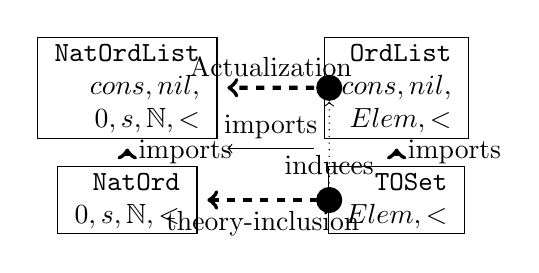
\begin{tikzpicture}[scale=.57]  \node (natordlist) at (0,2.5) 
    {\begin{tabular}{|r|}\hline 
      {\tt{NatOrdList}}\\
      $cons, nil,$\\
      $0,s,{\mathbb{N}},<$\\\hline
    \end{tabular}};
  \node (natord) at (0,0) 
    {\begin{tabular}{|r|}\hline 
      {\tt{NatOrd}}\\
      $0,s,{\mathbb{N}},<$\\\hline
    \end{tabular}};
  \node (toset) at (6,0) 
    {\begin{tabular}{|r|}\hline 
      {\tt{TOSet}}\\
      $Elem,<$\\\hline
    \end{tabular}};
  \node (ordlist) at (6,2.5) 
    {\begin{tabular}{|r|}\hline 
      {\tt{OrdList}}\\
      $cons, nil,$\\
      $Elem,<$\\\hline
    \end{tabular}};
  \node[circle,fill] (act1) at (4.5,2.5) {};
  \node[circle,fill] (act2) at (4.5,0) {};
  \draw [->,line width=1.5pt] (natord) -- node[right]{imports} (natordlist);
  \draw [->,line width=1.5pt] (toset) -- node[right]{imports} (ordlist);
  \draw [->,dashed,line width=1.5pt] (toset) -- node[below]{theory-inclusion} (natord);
  \draw [->,dashed,line width=1.5pt] (ordlist) -- node[above]{Actualization} (natordlist);
  \draw [->] (ordlist.south west) -- node[above]{imports} (natordlist.south east);
  \draw [<-,dotted,near end] (act1) -- node{induces} (act2);
\end{tikzpicture}
      \vspace*{-1.6cm}
    \end{minipage}\\[-1ex]\hline
 {\emph{Statement Level}:} 
    \begin{itemize}
    \item Axiom, definition, theorem, proof, example,\ldots
    \item Structure explicit in statement forms and references
    \end{itemize}&
{\footnotesize\baselineskip=10pt\strut\vspace*{-3ex}
\begin{lstlisting}[numbers=none,frame=none,mathescape]
<definition for="plus" type="recursive">
 <CMP><xhtml:p>Addition is defined by
   recursion on the second argument.</xhtml:p>
 </CMP>
 <FMP>$X+0=0$</FMP> 
 <FMP>$X+s(Y)=s(X+Y)$</FMP> 
</definition>
\end{lstlisting}}\\[-3ex]\hline
   {\emph{Object Level}:} {\openmath}/{\mathml}
    \begin{itemize}
    \item Objects as logical formulae
    \item Semantics by pointing to theory level
    \end{itemize} &
{\begin{minipage}[t]{5.4cm}\footnotesize\baselineskip=10pt\strut\vspace*{-3ex}
\begin{lstlisting}[numbers=none,frame=none]
<OMA>
 <OMS cd="arith1" name="plus"/>
 <OMV name="X"/>
 <OMS cd="nat" name="zero"/>
</OMA>
\end{lstlisting}\vspace{-3ex}\end{minipage}}\\\hline
\end{tabular}
\end{myfig}
Building on the discussion in {\mychapref{math-markup}} we distinguish three levels of
representation in {\omdoc}
\begin{description}
\item[\emph{Mathematical Theories} (see {\mysecref{math-objects}})] At this level,
  {\omdoc} supplies original markup for clustering sets of statements into theories, and
  for specifying relations between theories by morphisms. By using this scheme,
  mathematical knowledge can be structured into reusable chunks. Theories also serve as
  the primary notion of context in {\omdoc}, they are the natural target for the context
  aspect of formula and statement markup.
\item[\emph{Mathematical Statements} (see {\mysecref{meta-math}})] {\omdoc} provides
  original mark\-up infrastructure for making the structure of mathematical statements
  explicit.  Again, we have content and context markup aspects. For instance the
  definition in the right hand side of the second row of {\myfigref{nutshell}} contains an
  informal description of the definition as a first child and a formal description in the
  two recursive equations in the second and third children supported by the
  {\attribute{type}{definition}} attribute, which states that this is a recursive
  definition. The context markup in this example is simple: it states that this piece of
  markup pertains to a symbol declaration for the symbol {\snippetin{plus}} in the current
  theory (presumably the theory {\snippetin{arith1}}).
\item[\emph{Mathematical Formulae} (see {\mysecref{meta-theories}})] At the level of
  mathematical formulae, {\omdoc} uses the established standards
  {\openmath}~\cite{BusCapCar:2oms04} and {\cmathml}~\cite{CarIon:MathML03}.  These
  provide content markup for the structure of mathematical formulae and context markup in
  the form of URI references in the symbol representations (see {\mychapref{mobj}} for an
  introduction).
\end{description}
All levels are augmented by markup for various auxiliary information that is
present in mathematical documents, e.g. notation declarations, exercises,
experimental data, program code, etc.
\end{tsection}

\begin{tsection}[id=situating]{Situating the OMDoc Format}

  The space of representation languages for mathematical knowledge reaches from the input
  languages of {\twintoo{computer algebra}{system}s}\twin{algebra}{system} (CAS) to
  presentation markup languages for mathematical vernacular like {\TeX/\LaTeX}. We have
  organized some of the paradigmatic examples in a diagram mapping coverage (which kinds
  of mathematical knowledge can be expressed) against machine support (which services the
  respective software system can offer) in {\myfigref{situating}}.

\begin{myfig}{situating}{Situating Content Markup: Math. Knowledge Management}
  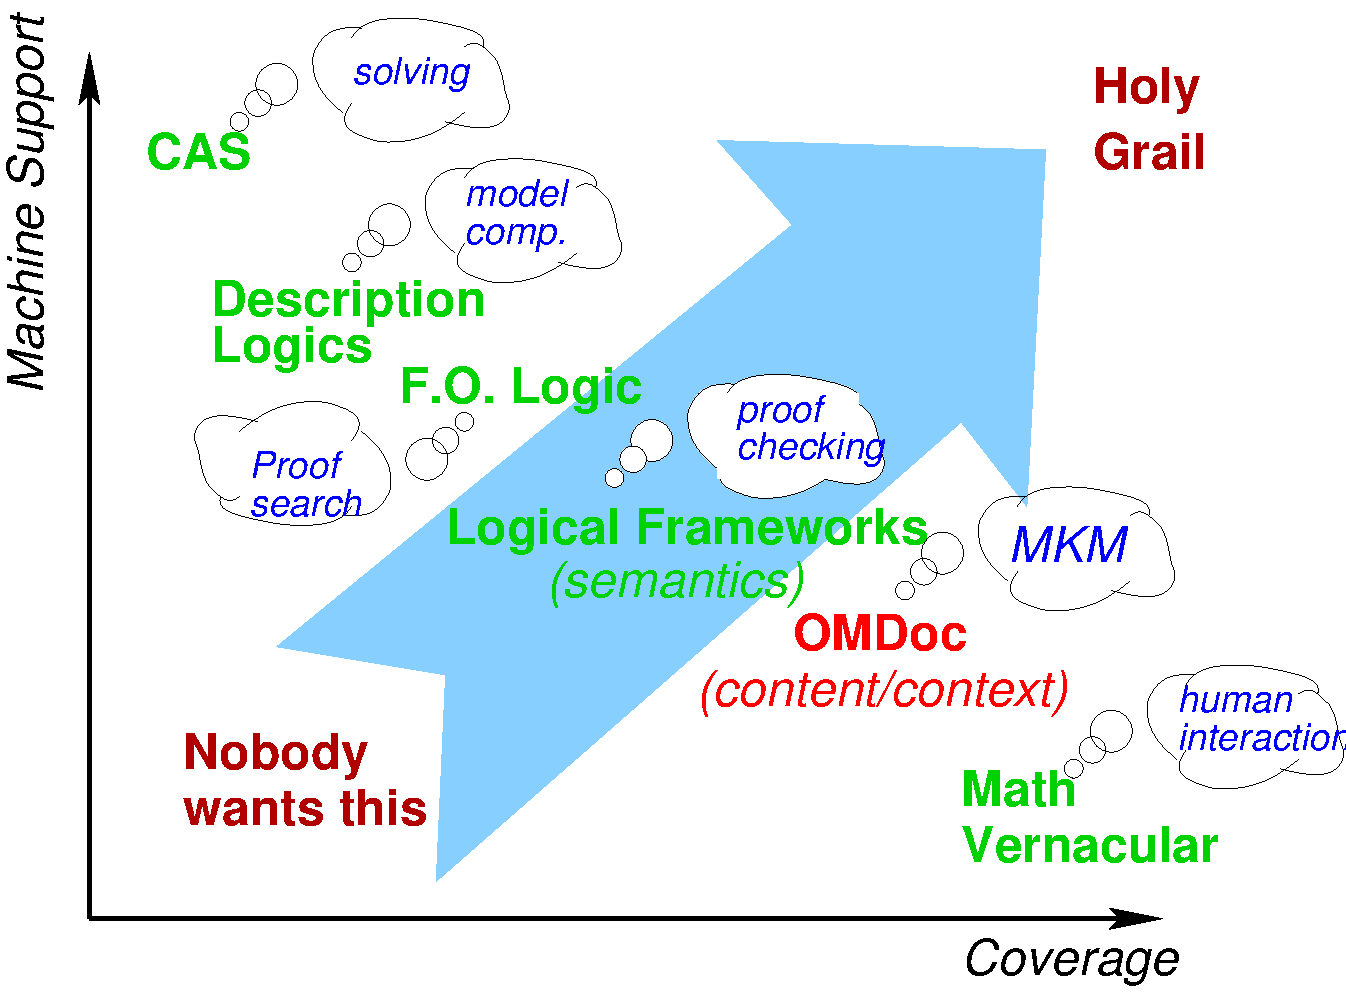
\includegraphics[width=11cm]{figures/support-coverage}
\end{myfig}

On the left hand side we see {\indextoo{CAS}} like {\mathematica}\cite{Wolfram.02} or
{\maple} {\cite{ChaGed:flatim92}} that are relatively restricted in the mathematical
objects --- they can deal with {\indextoo{polynomial}s}, {\indextoo{group
    representation}s}, {\twintoo{differential}{equation}s} only, but in this domain they
can offer sophisticated services like equation solving, factorization, etc.  More to the
right we see systems like {\indextoo{automated theorem prover}s}\index{theorem prover},
whose language --- usually {\twintoo{first-order}{logic}} --- covers much more of
mathematics, but that cannot perform computational services\footnote{Of course in
  principle, the systems could, since computation and theorem proving are inter-reducible,
  but in practice theorem provers get lost in the search spaces induced by computational
  tasks.}  like the CAS do.

In the lower right hand corner, we find languages like
``{\twintoo{mathematical}{vernacular}}'', which is just the everyday mathematical
language. Here coverage is essentially universal: we can use this language to write
international treaties, math books, and love letters; but machine support is minimal,
except for typesetting systems for mathematical formulae like {\TeX}, or keyword search in
the natural language part.

The distribution of the systems clusters around the diagonal stretching from low-coverage,
high-support systems like CAS to wide-coverage, low-support natural language systems. This
suggests that there is a trade-off between coverage and machine support. All of the
representation languages occupy legitimate places in the space of representation
languages, trying to find sweet-spots along this coverage/support trade-off. {\omdoc}
tries to occupy the ``{\twintoo{content}{markup}}'' position. To understand this position
better, let us contrast it to the ``{\twintoo{semantic}{markup}}'' position immediately to
the left of and above it. This is an important distinction, since it marks the border
between formal and {\twintoo{informal}{mathematics}}\twin{formal}{mathematics}.

We define a {\atwindef{semantic}{markup}{format}} (aka {\twindef{formal}{system}}) as a
representation system that has a way of specifying when a formula is a
{\indextoo{consequence}} of another. Many semantic markup formats express the
{\twintoo{consequence}{relation}} by means of a {\twintoo{formal}{calculus}}, which allows
the mechanization of {\twintoo{proof}{checking}} or {\twintoo{proof}{verification}}. It is
a widely held belief in mathematics, that all mathematical knowledge can in principle be
expressed in a {\twintoo{formal}{system}}, and various systems have been proposed and
applied to specific areas of mathematics. The advantage of having a well-defined
consequence relation (and proof-checking) has to be paid for by committing to a particular
logical system.

{\twindef{Content}{markup}} does not commit to a particular consequence relation, and
concentrates on providing services based on the marked up structure of the content and the
context.  Consider for instance the logical formula in {\mylstref{om-comm}}, where the
{\openmath} representation does not specify the full consequence relation (or the
{\twintoo{formal}{system}}) for the formula. It does something less but still useful,
which is what we could call {\twinemph{semantics by}{pointing}}: The symbols used in the
representation are identified by a pointer (the {\indextoo{URI}} jointly specified in the
{\attribute[ns-elt=om]{cd}{OMS}} and {\attribute[ns-elt=om]{name}{OMS}} attributes) to a
defining document (in this case an {\openmath} {\indextoo{content dictionary}}). Note that
URI equality is a sufficient condition for two symbols to be equal, but not a necessary
condition: Two symbols can be semantically equal without pointing to the same document,
e.g.  if the two defining documents are semantically marked up and the definitions are
semantic consequences of each other.

In this sense, content markup offers a more generic markup service (for all formal
systems; we do not have to commit ourselves) at the cost of being less precise (we for
instance miss out on some symbol equalities). Thus, {\twintoo{content}{markup}} is placed
to the lower right of {\twintoo{semantic}{markup}} in {\myfigref{situating}}.  Note
however, that content markup can easily be turned into semantic markup by adding a
consequence relation, e.g. by pointing to defining documents that are marked up
semantically.  Unlike {\openmath} and {\cmathml}, the {\omdoc} format straddles the
content/semantics border by closing the loop and providing a content markup format for
both formulae and the defining documents. In particular, {\emph{an {\omdoc} document is
    semantic if all the documents it references are}}.

As a consequence, {\omdoc} can serve as a {\twintoo{migration}{format}} from formal to
informal mathematics (and thus from representations that for human consumption to such
that can be supported by machines). A document collection can be marked for content and
context structure, making the structures and context references explicit in a first
pass. Note that this pass may involve creating additional documents or identifying
existing documents that serve as targets for the context references so that the document
collection is self-contained.  In a second (and possible semi-automatic) step, we can turn
this self-contained document collection into a formal representation (semantic markup) by
committing on consequence relations and adding the necessary detail to the referenced
documents.
\end{tsection}

\begin{tsection}[id=mathweb]{The Future: An Active Web of (Mathematical) Knowledge}
It is a crucial -- if relatively obvious -- insight that true cooperation of
mathematical services is only feasible if they have access to a joint corpus of
mathematical knowledge. Moreover, having such a corpus would allow to develop
added-value services like
\begin{itemize}
\item Cut and paste on the level of computation (take the output from a web search engine
  and paste it into a computer algebra system),
\item Automatically proof checking published proofs,
\item Math explanation (e.g. specializing a proof to an example that simplifies the proof
  in this special case),
\item Semantic search for mathematical concepts (rather than keywords),
\item Data mining for representation theorems (are there unnoticed groups out there?),
\item Classification: Given a concrete mathematical structure, is there a general theory
  for it?
\end{itemize}
As the online mathematical knowledge is presently only machine-{\emph{readable}}, but not
machine-{\emph{understandable}}, all of these services can currently only be performed by
humans, limiting the accessibility and thus the potential value of the
information. Services like this will transform the now passive and human-centered fragment
of the Internet that deals with mathematical content, into an active (supported by
semantic services) web of mathematical knowledge.

This promise of activating a web of knowledge is not limited to mathematics: the task of
transforming the current presentation-oriented world-wide web into a ``Semantic
Web''~\cite{BernersLee:tsw98} has been identified as one of the main challenges by the
world {\indextoo{W3C}}. With the {\omdoc} format we pursue an alternative vision of a
`Semantic Web' for Mathematics. Like {\twintoo{Tim}{Berners-Lee}}'s vision we aim to make
the Web (here mathematical knowledge) machine-understandable instead of merely
machine-readable. However, instead of a top-down metadata-driven approach, which tries to
approximate the content of documents by linking them to web ontologies (expressed in
terminologic logics), we explore a bottom-up approach and focus on making explicit the
intrinsic structure of the underlying scientific knowledge. A connection of documents to
web ontologies is still possible, but a secondary effect.

The direct applications of {\omdoc} (apart from the general effect towards a Semantic Web)
are not confined to mathematics proper either.  The {\mathml} working group in the W3C has
led the way in many web technologies (presenting mathematics on the web taxes the current
web technology to its limits); the endorsement of the {\mathml} standard by the W3
Committee is an explicit testimony to this. We expect that the effort of creating an
infrastructure for digital mathematical libraries will play a similar role, since
mathematical knowledge is the most rigorous and condensed form of knowledge and will
therefore pinpoint the problems and possibilities of the semantic web.

All modern sciences have a strongly mathematicised core and will benefit. The real market
and application area for the techniques developed in this project lies with high-tech and
engineering corporations that rely on huge formula databases.  Currently, both the content
markup as well as the added-value services alluded to above are very underdeveloped,
limiting the usefulness of vital knowledge. The content-markup aspect needed for mining
this information treasure is exactly what we are developing in {\omdoc}.
\end{tsection}
\end{tchapter}



%%% Local Variables: 
%%% mode: latex
%%% TeX-master: "omdoc"
%%% End: 

% LocalWords:  mobj arith cd nat mathescape eq comm rec om ns elt rpc Bundy th
% LocalWords:  CMP FMP OMA OMV CAS online metadata Andrzej Trybulec Berners


%%%%%%%%%%%%%%%%%%%%%%%%%%%%%%%%%%%%%%%%%%%%%%%%%%%%%%%%%%%%%%%%%%%%%%%%%
% This file is part of the LaTeX sources of the OMDoc 1.3 specification
% Copyright (c) 2006 Michael Kohlhase
% This work is licensed by the Creative Commons Share-Alike license
% see http://creativecommons.org/licenses/by-sa/2.5/ for details
%%%%%%%%%%%%%%%%%%%%%%%%%%%%%%%%%%%%%%%%%%%%%%%%%%%%%%%%%%%%%%%%%%%%%%%%%

\part{An OMDoc Primer}\label{part:primer}
This part of the {\report} provides an easily approachable description of the {\omdoc}
format by way of paradigmatic examples of {\omdoc} documents.  The primer should be used
alongside the formal descriptions of the language contained in
{\mypartref{specification}}.

The intended audience for the primer are users who only need a casual exposure to the
format, or authors that have a specific text category in mind.  The examples presented
here also serve as specifications of ``best practice'', to give the readers an intuition
for how to encode various kinds of mathematical knowledge.

Each chapter of the {\omdoc} primer deals with a different category of mathematical
document and introduces new features of the {\omdoc} format in the context of concrete
examples.

\paragraph{\Mychapref{algebra}: Mathematical Textbooks and Articles} discusses the markup
process for an informal but rigorous mathematical texts.  We will use a fragment of
Bourbaki's ``Algebra'' as an example.  The development marks up the content in four steps,
from the document structure to a full formalization of the content that could be used by
automated theorem provers.  The first page of Bourbaki's ``Algebra'' serves as an example
of the treatment of a rigorous presentation of pure mathematics, as it can be found in
textbooks and articles.

\paragraph{\Mychapref{omcds} OpenMath Content Dictionaries} transforms an {\openmath}
content dictionary into an {\omdoc} document. {\openmath} content dictionaries are
semi-formal documents that serve as references for mathematical symbols in {\openmath}
encoded formulae.  As of {\openmath}2, {\omdoc} is an admissible {\openmath} content
dictionary format. They are a good example for mathematical glossaries, and background
references, both formal and informal.

\paragraph{\Mychapref{natlist} Structured and Parametrized Theories} shows the power of
theory markup in {\omdoc} for theory reuse and modular specification. The example builds a
theory of ordered lists of natural numbers from a generic theory of ordered lists and the
theory of natural numbers which acts as a parameter in the actualization process.

\paragraph{\Mychapref{dg-elal} A Development Graph for Elementary Algebra} extends the
range of theory-level structure by specifying the elementary algebraic hierarchy. The rich
fabric of relations between these theories is made explicit in the form of theory
morphisms, and put to use for proof reuse.

\paragraph{\Mychapref{courseware} Courseware and the Narrative/Content Distinction}
covers markup for a fragment of a computer science course in the {\omdoc} format, dwelling
on the difference between the narrative structure of the course and the background
knowledge. Course materials like slides or writings on blackboards are usually much more
informal than textbook presentations of mathematics. They also openly structure materials
by didactic criteria and leave out important parts of the rigorous development, which the
student is required to pick up from background materials like textbooks or the teacher's
recitation.

\paragraph{\Mychapref{rpc} Communication with and between Mathematical Software Systems}
uses an {\omdoc} fragment as content for communication protocols between mathematical
software systems on the Internet.  Since the communicating parties in this situation are
machines, {\omdoc} fragments are embedded into other {\xml} markup that serves as a
protocol for the distribution layer.

\medskip 

Together these examples cover many of the mathematical documents involved in communicating
mathematics. As the first two chapters build upon each other and introduce features of the
{\omdoc} format, they should be read in succession.  The remaining three chapters build on
these, but are largely independent.

To keep the presentation of the examples readable, we will only present salient parts of
the {\omdoc} representations in the discussion. The full text of the examples can be
accessed at \url{https://svn.omdoc/repos/omdoc/doc/spec/examples/spec}.

%%% Local Variables: 
%%% mode: latex
%%% TeX-master: "omdoc"
%%% End: 

% LocalWords:  OMDoc omdoc
% LocalWords:  provers omdoc formulae omcds natlist xmlrpc rpc dg elal
%%%%% The primer part
%%%%%%%%%%%%%%%%%%%%%%%%%%%%%%%%%%%%%%%%%%%%%%%%%%%%%%%%%%%%%%%%%%%%%%%%%
% This file is part of the LaTeX sources of the OMDoc 1.3 specification
% Copyright (c) 2016 Michael Kohlhase.
% Source at https://github.com/KWARC/OMDoc/tree/master/doc/spec
% This work is licensed by the Creative Commons Share-Alike license
% see http://creativecommons.org/licenses/by-sa/2.5/ for details
%%%%%%%%%%%%%%%%%%%%%%%%%%%%%%%%%%%%%%%%%%%%%%%%%%%%%%%%%%%%%%%%%%%%%%%%%

\begin{tchapter}[id=algebra,short=Textbooks and Articles]{Mathematical Textbooks and Articles}

  In this chapter we will work an example of a stepwise formalization of mathematical
  knowledge. This is the task of e.g. an editor of a mathematical textbook preparing it
  for web-based publication.  We will use an informal, but rigorous text: a fragment of
  Bourbaki's Algebra~\cite{Bourbaki:a74}, which we show in {\myfigref{bourbaki}}. We will
  mark it up in four stages, discussing the relevant {\omdoc} elements and the design
  decisions in the {\omdoc} format as we go along.  Even though the text was actually
  written prior to the availability of the {\TeX/\LaTeX} system, we will take a {\LaTeX}
  representation as the starting point of our markup experiment, since this is the
  prevalent source markup format in mathematics nowadays.
\setbox1=\hbox{\cite{Bourbaki:a74}}
\begin{myfig}{bourbaki}{A fragment from Bourbaki's algebra~\usebox1}
\hspace*{-12pt}\fbox{\begin{minipage}{11cm}\small
      \noindent{\bf 1. LAWS OF COMPOSITION}\vspace{1em}\par\noindent
      {\sc Definition 1.} {\emph{Let $E$ be a set. A mapping of $E\times E$ is
        called a law of composition on $E$. The value $f(x,y)$ of $f$ for an
        ordered pair $(x,y)\in E\times E$ is called the composition of $x$ and $y$
        under this law. A set with a law of composition is called a magma.}}
      \vspace{1em}

      The composition of $x$ and $y$ is usually denoted by writing $x$ and $y$ in a
      definite order and separating them by a characteristic symbol of the law in question
      (a symbol which it may be agreed to omit). Among the symbols most often used are $+$
      and $\cdot$, the usual convention being to omit the latter if desired; with these
      symbols the composition of $x$ and $y$ is written respectively as $x+y$, $x.y$ or
      $xy$. A law denoted by the symbol $+$ is usually called {\emph{addition}} (the
      composition $x+y$ being called the {\emph{sum}} of $x$ and $y$) and we say that it
      is {\emph{written additively}}; a law denoted by the symbol $.$ is usually called
      {\emph{multiplication}} (the composition $x.y=xy$ being called the {\emph{product}}
      for $x$ and $y$) and we say that it is {\emph{written multiplicatively}}.
      
      In the general arguments of paragraphs 1 to 3 of this chapter we shall generally use
      the symbols $\top$ and $\bot$ to denote arbitrary laws of composition.
      
      By an abuse of language, a mapping of a {\emph{subset}} of $E\times E$ into $E$ is
      sometimes called a law of composition {\emph{not everywhere defined}} on $E$.
      \vspace{1em}

      \strut\hfill
      \begin{minipage}{11cm}\parindent=1.5em
        {\emph{Examples}}. (1) The mappings $(X,Y)\mapsto X\cup Y$ and $(X,Y)\mapsto
        X\cap Y$ are laws of composition on the set of subsets of a set $E$.
        
        (2) On the set $\bf N$ of natural numbers addition, multiplication, and
        exponentiation are laws of composition (the compositions of $x\in{\bf N}$
        and $y\in{\bf N}$ under these laws being denoted respectively by $x+y$,
        $xy$, or $x.y$ and $x^y$) ({\em{Set Theory}}, III, $\S3$, no. 4).
  
        (3) Let $E$ be a set; the mapping $(X,Y)\mapsto X\circ Y$ is a law of
        composition on the set of subsets of $E\times E$ ({\emph{Set Theory}}, II,
        $\S3$, no. 3, Definition 6); the mapping $(f,g)\mapsto f\circ g$ is a law
        of composition on the set of mappings from $E$ into $E$ ({\emph{Set Theory}},
        II, $\S5$, no. 2).
      \end{minipage}
    \end{minipage}}
\end{myfig}

{\Mysecref{minimal-omdoc}} discusses the minimal markup that is needed to turn an
arbitrary document into a valid {\omdoc} document --- albeit one, where the markup is
worthless of course. It discusses the necessary {\xml} infrastructure and adds some
meta-data to be used e.g. for {\twintoo{document}{retrieval}} or
archiving\twin{document}{archiving} purposes.

In {\mysecref{top-level}} we mark up the top-level structure of the text and
classify the paragraphs by their category as mathematical statements.  This level
of markup already allows us to annotate and extract some meta-data and would allow
applications to slice the text into individual units, store it in databases like
{\mbase} (see {\mysecref{mbase}}), or the In2Math knowledge
base~\cite{Dahn:sbt01,BauBlo:adtmpd01}, or assemble the text slices into
individualized books e.g. covering only a sub-topic of the original work.
However, all of the text itself, still contains the {\LaTeX} markup for formulae,
which is readable only by experienced humans, and is fixed in notation.  Based on
the segmentation and meta-data, suitable systems like the {\activemath} system
described in {\mysecref{activemath}} can re-assemble the text in different orders.
   
In {\mysecref{formulae}}, we will map all mathematical objects in the text into
{\openmath} or {\cmathml} objects. To do this, we have to decide which
symbols we want to use for marking up the formulae, and how to structure the
theories involved. This will not only give us the ability to generate specialized
and user-adaptive notation for them (see {\mychapref{transform-xsl}}), but also to
copy and paste them to symbolic math software systems. Furthermore, an assembly
into texts can now be guided by the semantic theory structure, not only by the
mathematical text categories or meta-data.
   
Finally, in {\mysecref{formalization}} we will fully formalize the mathematical
knowledge. This involves a transformation of the
{\twintoo{mathematical}{vernacular}} in the statements into some logical
formalism. The main benefit of this is that we can verify the mathematical
contents in theorem proving environments like {\nuprl}~\cite{Constable86},
{\hol}~\cite{GoMe93}, {\mizar}~\cite{Rudnicki:aomp92} and
OMEGA~\cite{BenzmuellerEtAl:otama97}.

\begin{tsection}[id=minimal-omdoc]{Minimal OMDoc Markup}

  It actually takes very little change to an existing document to make it a valid {\omdoc}
  document. We only need to wrap the text into the appropriate {\xml} document tags. In
  {\mylstref{outerpart}}, we have done this and also added
  {\indextoo{meta-data}}. Actually, since the {\element{metadata}} and the document type
  declaration are optional in {\omdoc}, just wrapping the original text with lines 1, 4,
  7, 31, 32, and 36 to 38 is the simplest way to create an {\omdoc}
  document.\medskip
\begin{lstlisting}[label=lst:outerpart,mathescape,
    caption={The outer part of the document},
    index={DOCTYPE,omdoc,metadata,dc:title,dc:creator,dc:date,dc:description,dc:source,
           dc:type,dc:format,theory,omtext,CMP}]
<?xml version="1.0" encoding="utf-8"?>
<!DOCTYPE omdoc PUBLIC "-//OMDoc//DTD OMDoc Basic V1.3//EN"
                "http://omdoc.org/dtd/omdoc-basic.dtd" []>

<omdoc xml:id="algebra1.omdoc" version="1.3" modules="@basic"
       xmlns:dc="http://purl.org/dc/elements/1.1/" 
       xmlns:cc="http://creativecommons.org/ns"
       xmlns="http://omdoc.org/ns">
  <metadata>
    <dc:title>Laws of Composition</dc:title>
    <dc:creator role="trl">Michael Kohlhase</dc:creator> 
    <dc:date action="created">2002-01-03T07:03:00</dc:date>
    <dc:date action="updated">2002-11-23T18:17:00</dc:date>
    <dc:description>
      A first migration step for a fragment of Bourbaki's Algebra
    </dc:description>
    <dc:source>
      Nicolas Bourbaki, Algebra, Springer Verlag 1989, ISBN 0-387-19373-1
    </dc:source>
    <dc:type>Text</dc:type>
    <dc:format>application/omdoc+xml</dc:format>
    <dc:rights>Copyright (c) 2005 Michael Kohlhase</dc:rights>
    <cc:license>
      <cc:permissions reproduction="permitted" distribution="permitted" 
                      derivative_works="permitted"/>
      <cc:prohibitions commercial_use="permitted"/>
      <cc:requirements notice="required" copyleft="required" attribution="required"/>
    </cc:license>
  </metadata>

  <omtext xml:id="all">
    <CMP xml:lang="en">
      <xhtml:p>
        {\sc Definition 1.} Let $E$ be a set. A mapping $E\times E$ is called a law of
        $\ldots$
        mappings from $E$ into $E$ ({\emph{Set Theory}}, II, $\S5$, no. 2).
      </xhtml:p>
    </CMP>
  </omtext>
</omdoc>
\end{lstlisting}\medskip

\noindent \renewcommand{\baselinestretch}{.97}We will now explain
the general features of the {\omdoc} representation in detail by
line numbers. The references point to the relevant sections in the
{\omdoc} specification; details and normative rules for using the
elements in questions can be found there.%\pagebreak

We will now explain the general features of the {\omdoc} representation in detail
by line numbers. The references point to the relevant sections in the {\omdoc}
specification; details and normative rules for using the elements in questions can
be found there.
\begin{small}
\begin{longtable}{|l|p{8.6cm}|p{.8cm}|}\hline
  line & Description & ref.\\\hline\hline
1 & This document is an {\xml} 1.0 file
  that is encoded in the {\twintoo{UTF-8}{encoding}}. 
  & \\\hline
2,3 & The parser is told to use a document type
       definition for validation. The string {\snippet{omdoc}} specifies the name of
       the root element, the identifier {\snippet{PUBLIC}} specifies that the DTD (we use
      the ``{\omdoc} basic'' DTD; see {\mysubsecref{sub-languages:basic}}),
      which can be identified by the {\twintoo{public}{identifier}} in the first string
      and looked up in an {\xml} catalog\twin{XML}{catalog} or (if that fails) can be 
      found at the URL specified in the second string. 

      A DTD declaration is not strictly needed for an {\omdoc} document, but is
      recommended, since the DTD supplies default values  for some attributes. 
  & {\ref{sec:validate-dtd}}  p.~\pageref{sec:validate-dtd}\\\hline
4 & In general, {\xml} files can contain as much whitespace as they want between elements,
    here we have used it for structuring the document. & \\\hline
5 & Start tag\twin{start}{tag} of the root element
    of the document. It declares the version ({\omdocv{1.3}}) via the
    {\attribute{version}{omdoc}}, and an identifier of the document using the
    {\attribute[ns-attr=xml]{id}{omdoc}} attribute. The optional {\attribute{modules}{omdoc}}
    specifies the sub-language used in this document. This is used when no DTD is present
    (see {\mysubsecref{sub-languages:basic}}).
  & {\ref{eldef:omdoc}}  p.~\pageref{eldef:omdoc}\\\hline
6,7 & the {\atwintoo{namespace}{prefix}{declaration}s} for the Dublin Core\twin{Dublin
    Core}{namespace}, Creative Commons\twin{Creative Commons}{namespace}, and
    {\openmath}\twin{OpenMath}{namespace} namespaces. They declare the prefixes
    {\snippetin{dc:}}, {\snippetin{cc:}}, and {\snippetin{om:}}, and bind them to the
    specified {\indextoo{URI}s}. We will need the {\openmath} namespace only in the
    third markup step described in {\mysecref{formulae}}, but spurious namespace prefix
    declarations are not a problem in  the {\xml} world. 
  & {\ref{chap:spec-intro}}  p.~\pageref{chap:spec-intro}\\\hline
8 & the {\twintoo{namespace}{declaration}} for the document; if not prefixed, all
    elements live in the {\omdoc} namespace\twin{OMDoc}{namespace}.
  & {\ref{sec:omdoc-ns}}  p.~\pageref{sec:omdoc-ns}\\\hline
9--29 & The {\indextoo{metadata}} for the whole document in Dublin Core
  format 
  & {\ref{eldef:metadata}}  p.~\pageref{eldef:metadata}\\\hline
10 & The title of the  document &\ref{eldef:dc:title} p.~\pageref{eldef:dc:title} \\\hline
11 & The document creator, here in the role of a {\indextoo{translator}}
  & {\ref{sec:dc-roles}}  p.~\pageref{sec:dc-roles}\\\hline
12 & The date and time of first creation of the document in {\atwintoo{ISO}{8601}{norm}}
    format.  & {\ref{eldef:dc:date}} p.~\pageref{eldef:dc:date} \\\hline
13 & The date and time of the last update to the document in {\atwintoo{ISO}{8601}{norm}}
    format. & {\ref{eldef:dc:date}} p.~\pageref{eldef:dc:date} \\\hline
14--16 & A short description of the contents of the document
   & {\ref{eldef:dc:description}} p.~\pageref{eldef:dc:description} \\\hline
17--19 & Here we acknowledge that the {\omdoc} document is just a translation from an
     earlier work. & {\ref{eldef:dc:source}} p.~\pageref{eldef:dc:source} \\\hline
20 & The type of the document, this can be {\snippetin{Dataset}} (un-ordered 
     mathematical knowledge) or {\snippetin{Text}} (arranged for human consumption). 
     & {\ref{eldef:dc:type}} p.~\pageref{eldef:dc:type} \\\hline
21 & The format/{\twintoo{MIME}{type}}~\cite{FreBor:MIME96} of the document, for {\omdoc}, this is
     {\snippetin{application/omdoc+xml}}. 
     & {\ref{eldef:dc:format}} p.~\pageref{eldef:dc:format} \\\hline
22 & The copyright resides with the creator of the {\omdoc} document
     & {\ref{eldef:dc:rights}} p.~\pageref{eldef:dc:rights} \\\hline
23--28 & The creator licenses the document to the world under certain conditions
     as specified in the {\twintoo{Creative Commons}{license}} specified in this element.
     & {\ref{eldef:cc:license}} p.~\pageref{eldef:cc:license} \\\hline
24,25 & The {\element[ns-elt=cc]{permissions}} element gives the world the {\indextoo{permission}} to
     reproduce\index{reproduction} and distribute\index{distribution} it
     freely. Furthermore the license grants the public the right to make derivative works
     under certain conditions.
     & {\ref{eldef:cc:permissions}} p.~\pageref{eldef:cc:permissions} \\\hline
26 & The {\element[ns-elt=cc]{prohibitions}} can be used to prohibit certain uses of the document,
     but this one is unencumbered.
     & {\ref{eldef:cc:prohibitions}} p.~\pageref{eldef:cc:prohibitions} \\\hline
27 & The {\element[ns-elt=cc]{requirements}} states conditions under which the license is
     granted. In our case the licensee is required to keep the copyright notice and
     license notices intact during distribution, to give credit to the copyright holder,
     and that any derivative works derived from this document must be licensed under the
     same terms as this document (the {\twintoo{copyleft}{clause}}).
     & {\ref{eldef:cc:requirements}} p.~\pageref{eldef:cc:requirements} \\\hline
31-37 & The {\element{omtext}} element  is used to mark up text fragments. Here, we
     have simply used a single {\element{omtext}} to classify the  whole text in the
     fragment as unspecific ``text''. 
   & {\ref{eldef:omtext}} p.~\pageref{eldef:omtext} \\\hline
32-36 & The {\element{CMP}} element holds the actual text in a
     {\twintoo{multilingual}{group}}. Its {\attribute[ns-attr=xml]{lang}{CMP}} specifies the language. 
     If the document is used with a {\indextoo{DTD}} or an {\xml} schema\twin{XML}{schema} (as we are)
     this attribute is redundant, since the default value given by the DTD or schema
     is {\attvalshort[ns-attr=xml]{en}{lang}}. More keywords in other languages can be given
     by adding more {\element{CMP}} elements.  
    & {\ref{eldef:CMP}} p.~\pageref{eldef:CMP} \\\hline
33--35 & The text of the {\LaTeX} fragment we are migrating. For simplicity we do
    not change the text, and leave that to later stages of the migration. & \\\hline
38 & The {\twintoo{closing}{tag}} of the root {\element{omdoc}}
     element. There may not be text after this in the file. 
   & {\ref{eldef:omdoc}} p.~\pageref{eldef:omdoc} \\\hline
\end{longtable}
\end{small}
\end{tsection}

\begin{tsection}[id=top-level,short=Structure and Statements]{Marking up the text
    structure and statements}
  
  In the next step, we analyze and mark up the structure of the text of the further, and
  embed the paragraphs into markup for mathematical statements or text segments.  Instead
  of lines 32--36 in {\mylstref{outerpart}}, we will now have the representation in
  {\mylstref{segmented-text}}.

\begin{lstlisting}[label=lst:segmented-text,mathescape,frame=topline,
    caption={The segmented text},
    index={theory,symbol,definition,omtext,CMP,omgroup,metadata,dc:title,example}]
<omtext xml:id="magma.def" type="definition">
  <CMP>
    <xhtml:p>Let <legacy format="TeX">$E$</legacy> be a set $\ldots$ called a magma.</xhtml:p>
  </CMP>
</omtext>

<omtext xml:id="t1">
  <CMP>
    <xhtml:p>The composition of <legacy format="TeX">$x$</legacy> $\ldots$
    multiplicatively.<xhtml:p>
   </CMP>
</omtext>
<omtext xml:id="t2">
  <CMP><xhtml:p>In the general $\ldots$ composition.<xhtml:p></CMP>
</omtext>
<omtext xml:id="t3">
  <CMP><xhtml:p>By an abuse $\ldots$ on <legacy format="TeX">$E$.</legacy></xhtml:p></CMP>
</omtext> 

<omgroup xml:id="magma-ex" type="enumeration">
   <metadata><dc:title>Examples</dc:title></metadata>

   <omtext type="example" xml:id="e1.magma">
     <CMP>
       <xhtml:p>
         The mappings <legacy format="TeX">$(X,Y)$</legacy> 
         $\ldots$ subsets of a set <legacy format="TeX">$E$</legacy>.
       </xhtml:p>
     </CMP>
   </omtext>
   <omtext type="example" xml:id="e2.magma">
     <CMP>
       <xhtml:p>
        On the set <legacy format="TeX">$\bf N$</legacy> $\ldots$ III, $\S3$, no. 4).
       </xhtml:p>
     </CMP>
   </omtext>
   <omtext type="example" xml:id="e3.magma">
     <CMP>
       <xhtml:p>Let <legacy format="TeX">$E$</legacy> be a set; $\ldots$ II, $\S5$, no. 2).</xhtml:p>
     </CMP>
   </omtext>
</omgroup>
\end{lstlisting}

In summary, we have sliced\index{slicing} the text into {\element{omtext}} fragments and
individually classified them by their mathematical role. The formulae inside have been
encapsulated into {\element{legacy}} elements that specify their format for further
processing. The {\twintoo{higher-level}{structure}} has been captured in {\omdoc} grouping
elements and the document as well as some of the slices have been annotated by metadata.
\begin{small}
\begin{longtable}{|l|p{8.6cm}|p{.8cm}|}\hline
  line & Description & ref.\\\hline\hline
1 & The {\element{omtext}} element classifies the text fragment as  a
    {\attval{definition}{type}{omtext}}, other types for mathematical statements include 
    {\attval{axiom}{type}{omtext}}, {\attval{example}{type}{omtext}},
    {\attval{theorem}{type}{omtext}}, and {\attval{lemma}{type}{omtext}}. Note that the
    numbering of the original text is lost, but can be re-created in the text presentation
    process. The optional {\attribute[ns-attr=xml]{id}{omtext}} attribute specifies a
    document-unique identifier that can be used for reference later. 
    &\ref{eldef:omtext} p.~\pageref{eldef:omtext}\\\hline
2 & A {\twintoo{multilingual}{group}} of {\element{CMP}} elements that hold the  text (in our
    case, there is only the English default). Here
    the {\TeX} formulae have been marked up with {\element{legacy}} elements
    characterizing them as such. This might simplify a later
    automatic transformation to {\openmath} or {\cmathml}.
  & {\ref{eldef:legacy}} p.~\pageref{eldef:legacy} \\\hline
4--13 & We have classified every paragraph in the original as a separate
   {\element{omtext}} element, which does not carry a {\attribute{type}{omtext}} since it
   does not fit any other mathematical category at the moment. 
   & {\ref{eldef:omtext}} p.~\pageref{eldef:omtext} \\\hline
15 & The three examples in the original in {\myfigref{bourbaki}} are grouped into
   an enumeration. We use the {\omdoc}  {\element{omgroup}} element for this. The
   optional attribute {\attribute[ns-attr=xml]{id}{omgroup}} can be used for referencing later. We have chosen
   {\attval{enumeration}{type}{omgroup}} for the {\attribute{type}{omgroup}}
   attribute to specify the numbering of the examples in the original.
   & {\ref{eldef:omgroup}}  p.~\pageref{eldef:omgroup} \\\hline
16 & We can use the {\element{metadata}} of the {\element{omgroup}} element to
   accommodate the title ``Examples'' in the original. We could enter more metadata
   at this level.   & {\ref{eldef:dc:title}} p.~\pageref{eldef:dc:title} \\\hline
18 & The {\attribute{type}{omtext}} attribute of this {\element{omtext}} element
     classifies this text fragment as an example.
   & {\ref{eldef:omtext}} p.~\pageref{eldef:omtext} \\\hline
 \end{longtable}
\end{small}
\end{tsection}

\begin{tsection}[id=formulae]{Marking up the Formulae}
 
  After we have marked up the top-level structure of the text to expose the content, the
  next step will be to mark up the formulae in the text to content mathematical form. Up
  to now, the formulae were still in {\TeX} notation, which can be read by {\TeX}/{\LaTeX}
  for presentation to the human user, but not used by symbolic mathematics software. For
  this purpose, we will re-represent the formulae as {\openmath} objects or {\cmathml},
  making their functional structure\twin{abstract}{syntax}\twin{structure}{abstract}
  explicit.

  So let us start turning the {\TeX} formulae in the text into {\openmath} objects. Here
  we use the hypothetical {\url{mbc.mathweb.org}} as repository for theory collections.

\begin{lstlisting}[label=lst:formulae-definition,mathescape,
    caption={The definition of a magma with {\openmath} objects},
    index={definition,CMP,om:OMOBJ,om:OMS,om:OMA,om:OMV}]
<!DOCTYPE omdoc PUBLIC "-//OMDoc//DTD OMDoc CD V1.3//EN" 
                       "http://omdoc.org/dtd/omdoc-cd.dtd" 
          [<!ENTITY % om.prefixed "INCLUDE">]>

<theory xml:id="magmas">
  <imports from="background.omdoc#products"/>
  <imports from="http://mbc.mathweb.org/omstd/relation1.omdoc#relation1"/>

  <symbol name="magma">
    <metadata><dc:description>Magma</dc:description></metadata>
  </symbol>
  <symbol name="law_of_composition"/>

  <definition xml:id="magma.def" for="magma law_of_composition">
    <CMP> 
     <xhtml:p>
      Let <om:OMOBJ><om:OMV name="E"/></om:OMOBJ> be a set. A mapping of 
      <om:OMOBJ>
        <om:OMA><om:OMS cd="products" name="Cartesian-product"/>
          <om:OMV name="E"/><om:OMV name="E"/>
        </om:OMA>
      </om:OMOBJ> is called a 
      <term cd="magmas" name="magma" role="definiendum">law of composition</term>
      on <om:OMOBJ><om:OMV name="E"/></om:OMOBJ>.  The value 
      <om:OMOBJ>
        <om:OMA><om:OMV name="f"/>
          <om:OMV name="x"/><om:OMV name="y"/>
        </om:OMA>
      </om:OMOBJ>
      of <om:OMOBJ><om:OMV  name="f"/></om:OMOBJ> for an ordered pair
      <om:OMOBJ>
        <om:OMA><om:OMS cd="sets" name="in"/>
          <om:OMA><om:OMS cd="products" name="pair"/>
            <om:OMV name="x"/><om:OMV name="y"/>
          </om:OMA>
          <om:OMA><om:OMS cd="products" name="Cartesian-product"/>
            <om:OMV name="E"/><om:OMV name="E"/>
          </om:OMA>
        </om:OMA>
      </om:OMOBJ> is called the 
      <term cd="magmas" name="law_of_composition" 
                        role="definiendum-applied">composition</term>
       of <om:OMOBJ><om:OMV name="x"/></om:OMOBJ> and 
      <om:OMOBJ><om:OMV name="y"/></om:OMOBJ> under this law. 
      A set with a law of composition is called a 
      <term cd="magmas" name="magma" role="definiendum">magma</term>.
      </xhtml:p>
    </CMP>
  </definition>
$\ldots$
</theory>
$\ldots$
\end{lstlisting}

Of course all the other mathematical statements in the documents have to be treated in the
same way.
\begin{small}
\begin{longtable}{|l|p{8.6cm}|p{.8cm}|}\hline
  line & Description & ref.\\\hline\hline 
  1--4 & The {\snippetin{omdoc-basic}} {\twintoo{document type}{definition}} is no longer
      sufficient for our purposes, since we introduce new symbols that can be used in
      other documents. The  {\indextoo{DTD}} for {\omdoc} content
      dictionaries\twin{content dictionary}{OMDoc} (see {\mychapref{omcds}}),
      which allows this. Correspondingly, we would specify the value
      {\attval{cd}{module}{omdoc}} for the attribute {\attribute{module}{omdoc}}.

      The part in line 4 is the {\twintoo{internal}{subset}} of the {\indextoo{DTD}},
      which sets a {\twintoo{parameter}{entity}} for the modularized DTD to instruct it to
      accept {\openmath} elements in their {\twintoo{namespace}{prefixed}} form. Of course
      a suitable {\twintoo{namespace prefix}{declaration}} is needed as well. 
     & {\ref{subsec:sub-languages:cd}} p.~\pageref{subsec:sub-languages:cd} \\\hline
  5   & The {\twintoo{start}{tag}} of a theory. We need this, since symbols and
       definitions  can only appear inside {\element{theory}} elements.  
       & {\ref{sec:theories}} p.~\pageref{sec:theories}\\\hline 
  6,7 & We need to import the theory {\snippet{products}} to  be able to use symbols
          from it in the definition below. The  value of the {\attribute{from}{imports}}
          is a relative {\twintoo{URI}{reference}} to a {\element{theory}} element much
          like the one in line  5. The other
          {\element{imports}} element imports the theory {\snippet{relation1}} from the
          {\openmath} standard content dictionaries\index{content dictionary}\footnote{The
            originals are available at 
            \url{http://www.openmath.org/cd}; see {\mychapref{omcds}} for a discussion
            of the differences of the original {\openmath} format and the {\omdoc}
            format used here.}.  Note that we do not need to import the theory
          {\snippet{sets}} here, since this is already imported by
      the theory {\snippet{products}}. 
    & {\ref{eldef:imports}} p.~\pageref{eldef:imports}\\\hline 
9--11 & A symbol declaration: For every definition, {\omdoc} requires the declaration of
        one or more {\element{symbol}} elements for the concept that is to be defined. The
        {\attribute{name}{symbol}} attribute is used to identify 
        it.  The {\element[ns-elt=dc]{description}} element allows to supply a multilingual (via the
        {\attribute[ns-attr=xml]{lang}{description}} attribute) group of keywords for the
        declared symbol 
     & {\ref{eldef:symbol}} p.~\pageref{eldef:symbol}\\\hline 
  12 & Upon closer inspection it turns out that the definition in
       {\mylstref{formulae-definition}} actually defines three concepts: ``law of
       composition'', ``composition'', and ``magma''. Note that ``composition'' is just
       another name for the value under the law of composition, therefore we do not need
       to declare a symbol for this. Thus we only declare one for ``law of composition''.
     & {\ref{eldef:symbol}} p.~\pageref{eldef:symbol}\\\hline 
  14 & A definition: the {\element{definition}} element carries a
       {\attribute{name}{definition}} attribute for reference within the theory. We need
       to reference the two symbols defined here in the {\attribute{for}{definition}} attribute 
       of the  {\element{definition}} element; it takes a whitespace-separated list of
      {\attribute{name}{symbol}} attributes of {\element{symbol}} elements in the same 
      theory as values.  
    & {\ref{eldef:definition}} p.\pageref{eldef:definition} \\\hline 
  16 & We use an {\openmath} object for the set $E$. It is an
      {\element[ns-elt=om]{OMOBJ}} element with an {\element[ns-elt=om]{OMV}} daughter, whose
      {\attribute{name}{OMV}} attribute specifies the object to be a variable with
      name $E$. We have chosen to represent the set $E$ as a variable instead of a
      constant (via an {\element[ns-elt=om]{OMS}} element) in the theory, since it seems to be
      local to the definition. We will discuss this further in the next section, where
      we talk about formalization.  
    & {\ref{eldef:om:OMOBJ}} p.~\pageref{eldef:om:OMOBJ} \\\hline 
  17--21 & This {\element[ns-elt=om]{OMOBJ}} represents the {\twintoo{Cartesian}{product}}
          $E\times E$ of the set $E$ with itself.
      It is an application (via an {\element[ns-elt=om]{OMA}} element) of the symbol for the
      binary Cartesian product {\indextoo{relation}} to $E$.  
    & {\ref{eldef:om:OMA}} p.~\pageref{eldef:om:OMA} \\\hline 
  18 & The symbol for the Cartesian product
       {\indextoo{constructor}} is represented as an {\element[ns-elt=om]{OMS}} element. The
       {\attribute{cd}{OMS}} attribute specifies the theory that defines the symbol,
       and the {\attribute{name}{OMS}} points to the {\element{symbol}} element in it
       that declares this symbol. The value of the {\attribute{cd}{OMS}} attribute is a
       theory identifier. Note that this theory has to be imported into the
       current theory, to be legally used.
     & {\ref{eldef:om:OMS}} p.~\pageref{eldef:om:OMS}\\\hline 
   22 & We use the {\element{term}} element to characterize the defined terms in the text
        of the definition.  Its {\attribute{role}{term}} attribute can used to mark the
        text fragment as a {\attval{definiens}{role}{term}}, i.e. a concept that is under
        definition.   
      & {\ref{eldef:term}} p.~\pageref{eldef:term}\\\hline 
24--28 & This object stands   for $f(x,y)$ &  \\\hline 
30--39 & This object represents $(x,y)\in E\times E$.
         Note that we make use of the symbol for the elementhood relation from the
         {\openmath} core {\indextoo{content dictionary}} {\snippet{set1}} and of the
         {\indextoo{pair}{constructor}} from the theory of
         products from the Bourbaki collection there.  & \\\hline
\end{longtable}
\end{small}
\noindent The rest of the representation in
{\mylstref{formulae-definition}} is analogous. Thus we have treated
the first definition in {\myfigref{bourbaki}}. The next two
paragraphs contain notation conventions that help the human reader
to understand the text. They are annotated as {\element{omtext}}
elements. The third paragraph is really a definition (even if the
wording is a bit bashful), so we mark it up as one in the style of
{\mylstref{formulae-definition}} above.

Finally, we come to the examples at the end of our fragment. In the markup shown
in {\mylstref{example-formulae}} we have decided to construct a new theory for
these examples since the examples use concepts and symbols that are independent of
the theory of magmas. Otherwise, we would have to add the {\element{imports}}
element to the theory in {\mylstref{formulae-definition}}, which would have
mis-represented the actual dependencies. Note that the new theory has to import
the theory {\snippet{magmas}} together with the theories from which examples are taken,
so their symbols can be used in the examples. 
\begin{lstlisting}[label=lst:example-formulae,mathescape,
    caption={Examples for magmas with {\openmath} objects},
    index={example,CMP,OMOBJ,OMBIND,OMS,OMA,OMV}]
<theory xml:id="magmas-examples">
  <metadata><dc:title>Examples</dc:title></metadata>

   <imports from="http://mbc.mathweb.org/omstd/fns1.omdoc##fns1"/>
   <imports from="background.omdoc#nat"/>
   <imports from="background.omdoc#functions"/>
   <imports from="#magmas"/>
   
  <omgroup xml:id="magma-ex" type="enumeration">
    <metadata><dc:title>Examples</dc:title></metadata>

    <example xml:id="e1.magma" for="#law_of_composition" type="for">
      <CMP>The mappings 
        <xhtml:p>
        <om:OMOBJ>
          <om:OMBIND><om:OMS cd="fns1" name="lambda"/>
            <om:OMBVAR>
              <om:OMV name="X"/><om:OMV name="Y"/>
            </om:OMBVAR>
            <om:OMA><om:OMS cd="functions" name="pattern-defined"/>
              <om:OMA><om:OMS cd="products" name="pair"/>
                <om:OMV name="X"/>
                <om:OMV name="Y"/>
              </om:OMA>
              <om:OMA><om:OMS cd="sets" name="union"/>
                <om:OMV name="X"/>
                <om:OMV name="Y"/>
              </om:OMA>
            </om:OMA>
          </om:OMBIND>
        </om:OMOBJ> and 
        <om:OMOBJ>
          <om:OMBIND><om:OMS cd="fns1" name="lambda"/>
            <om:OMBVAR>
              <om:OMV name="X"/><om:OMV name="Y"/>
            </om:OMBVAR>  
            <om:OMA><om:OMS cd="functions" name="pattern-defined"/>
              <om:OMA><om:OMS cd="products" name="pair"/>
                <om:OMV name="X"/>
                <om:OMV name="Y"/>
              </om:OMA>
              <om:OMA><om:OMS cd="sets" name="intersection"/>
                <om:OMV name="X"/>
                <om:OMV name="Y"/>
              </om:OMA>
            </om:OMA>
          </om:OMBIND>
        </om:OMOBJ>
        are <term cd="magmas" name="law_of_composition>laws of composition</term>
        on the set of subsets of a set 
        <om:OMOBJ><om:OMS cd="magmas" name="E"/></om:OMOBJ>.
        </xhtml:p>
      </CMP>
    </example>
    
    <example xml:id="e2.magma" for="#law_of_composition" type="for">
      <CMP>
       <xhtml:p>
        On the set <om:OMOBJ><om:OMS cd="nat" name="Nat"/></om:OMOBJ> 
        of <term cd="nats" name="nats">natural numbers</term>, 
        <term cd="nats" name="plus">addition</term>, 
        <term cd="nats" name="times">multiplication</term>, and 
        <term cd="nats" name="power">exponentiation</term> are $\ldots$
       </xhtml:p>
      </CMP>
    </example>
  </omgroup>
</theory>
\end{lstlisting}

\noindent The {\element{example}} element in line 13 is used for
mathematical examples of a special form in {\omdoc}: objects that
have or fail to have a specific property. In our case, the two given
mappings have the property of being a law of composition. This
structural property is made explicit by the
{\attribute{for}{example}} attribute that points to the concept that
these examples illustrate, in this case, the symbol
{\snippet{law\_of\_composition}}. The {\attribute{type}{example}}
attribute has the values {\attval{for}{type}{example}} and
{\attval{against}{type}{example}}.  In our case
{\attval{for}{type}{example}} applies,
{\attval{against}{type}{example}} would for counterexamples. The
content of an {\element{example}} is a multilingual {\element{CMP}}
group. For examples of other kinds --- e.g. usage examples, {\omdoc}
does not supply specific markup, so we have to fall back to using an
{\element{omtext}} element with type
{\attval{example}{type}{omtext}} as above.

In our text fragment, where the examples are at the end of the section that deals
with magmas, creating an independent theory for the examples (or even multiple
theories, if examples from different fields are involved) seems appropriate. In
other cases, where examples are integrated into the text, we can equivalently embed
theories into other theories. Then we would have the following structure:

\begin{lstlisting}[label=lst:example-embedded,mathescape,
    caption={Examples embedded into a theory},
    index={theory,imports}]
<theory xml:id="magmas">
  <imports xml:id="imp3" from="background.omdoc#products"/>
  <imports from="http://mbc.mathweb.org/omstd/relation1.omdoc#relation1"/>
  $\ldots$
  <theory xml:id="magmas-examples"
    <imports xml:id="imp4" 
       from="http://omdoc.org/examples/omstd/fns1.omdoc#fns1"/>
    <imports xml:id="imp5" from="background.omdoc#nat"/>
    <imports xml:id="imp6" from="background.omdoc#functions"/>
    $\ldots$
  </theory>
  $\ldots$
</theory>
\end{lstlisting}
Note that the embedded theory ({\snippet{magmas-examples}}) has access to all the
symbols in the embedding theory ({\snippet{magmas}}), so it does not have to import it.
However, the symbols imported into the embedded theory are only visible in it, and do
not get imported into the embedding theory.
\end{tsection}

\begin{tsection}[id=formalization]{Full Formalization}
      
  The final step in the migration of the text fragment involves a transformation of the
  {\twintoo{mathematical}{vernacular}} in the statements into some logical formalism. The
  main benefit of this is that we can verify the mathematical contents in theorem proving
  environments.  We will start out by dividing the first definition into two parts. The
  first one defines the symbol {\snippet{law\_of\_composition}}
  (see~\mylstref{law_of_composition-formal}), and the second one {\snippet{magma}}
  (see~\mylstref{magma:formal}).

\begin{lstlisting}[label=lst:law_of_composition-formal,
    caption={The formal definition of a law of composition},
    index={definition,CMP,OMOBJ,OMBIND,OMBVAR,OMS,OMA,OMV}]
<symbol name="law_of_composition">
  <metadata><dc:description>A law of composition on a set.</dc:description></metadata>
</symbol>
<definition xml:id="magma.def" for="law_of_composition" type="simple">
  <CMP> 
    <xhtml:p>
      Let <om:OMOBJ><om:OMV name="E"/></om:OMOBJ> be a set. A mapping of 
     <om:OMOBJ><om:OMR href="#comp.1"/></om:OMOBJ> 
     is called a <term cd="magmas" name="law_of_composition" 
                               role="definiens">law of composition</term>
     on <om:OMOBJ><om:OMV name="E"/></om:OMOBJ>.
   </xhtml:p>
  </CMP>
  <om:OMOBJ>
    <om:OMBIND>
      <om:OMS cd="fns1" name="lambda"/>
      <om:OMBVAR>
        <om:OMV name="E"/><om:OMV name="F"/>
      </om:OMBVAR>
      <om:OMA><om:OMS cd="pl0" name="and"/>
       <om:OMA><om:OMS cd="sets" name="set"/>
          <om:OMV name="E"/>
       </om:OMA>
       <om:OMA>
         <om:OMS cd="functions" name="function"/>
         <om:OMA id="comp.1">
           <om:OMS cd="products" name="Cartesian-product"/>
           <om:OMV name="E"/>
           <om:OMV name="E"/>
         </om:OMA>
         <om:OMV name="E"/>
       </om:OMA>
     </om:OMA>
   </om:OMBIND>
 </om:OMOBJ>
</definition>
\end{lstlisting}

\noindent The main difference of this definition to the one in the
section above is the {\element[ns-elt=om]{OMOBJ}} element, which now
accompanies the {\element{CMP}} element. It contains a formal
definition of the property of being a law of composition in the form
of a $\lambda$-term $\lambda{E,F}.set(E)\wedge F:E\times E\to
E$\footnote{We actually need to
  import the theories {\snippet{pl1}} for {\twintoo{first-order}{logic}} (it imports
  the theory {\snippet{pl0}}) to legally use the logical symbols here. Since we did not
  show the theory element, we assume it to contain the relevant {\element{imports}}
  elements.}. The value {\attval{simple}{type}{definition}} of the
{\attribute{type}{definition}} attribute in the {\element{definition}} element signifies
that the content of the {\element[ns-elt=om]{OMOBJ}} element can be substituted for the symbol
{\snippet{law\_of\_composition}}, wherever it occurs. So if we have
$\snippet{law\_of\_composition}(A,B)$ somewhere this can be reduced to
$(\lambda{E,F}.set(E)\wedge F:E\times E\to E)(A,B)$ which in turn reduces\footnote{We use
  the $\lambda$-calculus as a formalization framework here: If we
  apply a $\lambda$-term of the form $\lambda{X}.A$ to an argument $B$, then the result is
  obtained by binding all the formal parameters $X$ to the actual parameter $B$, i.e. the
  result is the value of $A$, where all the occurrences of $X$ have been replaced by $B$.
  See~\cite{Barendregt80,Andrews02} for an introduction.} to $set(A)\wedge B:A\times A\to
A$ or in other words $\snippet{law\_of\_composition}(A,B)$ is true, iff $A$ is a set and
$B$ is a function from $A\times A$ to $A$. This definition is directly used in the second
formal definition, which we depict in {\mylstref{magma:formal}}.

\begin{lstlisting}[label=lst:magma:formal,
    caption={The formal definition of a magma},
    index={definition,CMP,FMP,OMOBJ,OMS,OMA,OMV}]
 <definition xml:id="magma.def" for="magma" type="implicit">
  <CMP>
    <xhtml:p>
      A set with a law of composition is called a 
      <term cd="magmas" name="magma" role="definiendum">magma</term>.
    </xhtml:p>
  </CMP>
  <FMP>
    <om:OMOBJ>
      <om:OMBIND><om:OMS cd="pl1" name="forall"/>
        <om:OMBVAR><om:OMV name="M"/></om:OMBVAR>
        <om:OMA><om:OMS cd="pl0" name="iff"/>
          <om:OMA><om:OMS cd="magmas" name="magma"/>
            <om:OMV name="M"/>
          </om:OMA>
          <om:OMBIND>
            <om:OMS cd="pl1" name="exists"/>
            <om:OMBVAR>
              <om:OMV name="E"/><om:OMV name="C"/>
            </om:OMBVAR>
            <om:OMA><om:OMS cd="pl0" name="and"/>
              <om:OMA><om:OMS cd="relation1" name="eq"/>
                <om:OMV name="M"/>
                <om:OMA><om:OMS cd="products" name="Cartesian-product"/>
                  <om:OMV name="E"/>
                  <om:OMV name="C"/>
                </om:OMA>
              </om:OMA>
              <om:OMA><om:OMS cd="magmas" name="law_of_composition"/>
                <om:OMV name="E"/>
                <om:OMV name="F"/>
              </om:OMA>
            </om:OMA>
          </om:OMBIND>
        </om:OMA>
      </om:OMBIND>
    </om:OMOBJ>
  </FMP>
</definition>
\end{lstlisting}

\noindent Here, the {\attribute{type}{definition}} attribute on the
{\element{definition}} element has the value
{\attval{implicit}{type}{definition}}, which signifies that the
content of the {\element{FMP}} element should be understood as a
logical formula that is made true by exactly one object: the
property of being a {\indextoo{magma}}. This formula can be written
as
\[\allcdot{M}{magma(M)\Leftrightarrow\excdot{E,F}{M=(E,F)\land law\_of\_composition(E,F)}}\]
in other words: $M$ is a magma, iff it is a pair $(E,F)$, where $F$ is a law of
composition over $E$.

Finally, the examples get a formal part as well. This mainly consists of formally
representing the object that serves as the example, and making the way it does
explicit. The first is done simply by adding the object to the example as a
sibling node to the CMP. Note that we are making use of the {\openmath} reference
mechanism here that allows to copy subformulae by linking them with an
{\element[ns-elt=om]{OMR}} element that stands for a copy of the object pointed to by the
{\attribute{href}{OMR}} attribute (see {\mysecref{openmath}}), which makes
this very simple. Also note that we had to split the example into two, since
{\omdoc} only allows one example per {\element{example}} element. However, the
{\element{example}} contains two {\element[ns-elt=om]{OMOBJ}} elements, since the property of
being a law of composition is binary. 

The way this object is an example is made explicit by adding an assertion that makes the
claim of the example formal (in our case that for every set $E$, the function
$(X,Y)\mapsto X\cup Y$ is a law of composition on the set of subsets of $E$). The
assertion is referenced by the {\attribute{assertion}{example}} attribute in the
{\element{example}} element.

\begin{lstlisting}[label=lst:magma-formal-examples,frame=topline,
    caption={A  formalized magma example},
    index={example,assertion,CMP,FMP,OMOBJ,OMS,OMA,OMV}]
<example xml:id="e11.magma" for="#law_of_composition" 
         type="for" assertion="e11.magma.ass">
  <CMP>
    <xhtml:p>
      The mapping <om:OMOBJ><om:OMR href="#e11.magma.1"/></om:OMOBJ> is 
      a law of composition on the set of subsets of a set 
      <om:OMOBJ><om:OMS cd="magmas" name="E"/></om:OMOBJ>.
    </xhtml:p>
  </CMP>
  <om:OMOBJ>
    <om:OMA id="e11.magma.2"><om:OMS cd="sets" name="subset"/>
      <om:OMV name="E"/>
    </om:OMA>
  </om:OMOBJ>
  <om:OMOBJ>
    <om:OMBIND id="e11.magma.1">
      <om:OMS cd="fns1" name="lambda"/>
      <om:OMBVAR><om:OMV name="X"/><om:OMV name="Y"/></om:OMBVAR>
      <om:OMA>
        <om:OMS cd="functions" name="pattern-defined"/>
        <om:OMA><om:OMS cd="products" name="pair"/>
          <om:OMV name="X"/>
          <om:OMV name="Y"/>
        </om:OMA>
        <om:OMA><om:OMS cd="sets" name="union"/>
          <om:OMV name="X"/>
          <om:OMV name="Y"/>
        </om:OMA>
      </om:OMA>
    </om:OMBIND>
  </om:OMOBJ>
</example>

<assertion xml:id="e11.magma.ass">
  <FMP>
    <om:OMOBJ>
      <om:OMBIND>
        <om:OMS cd="pl1" name="forall"/>
        <om:OMBVAR><om:OMV name="E"/></om:OMBVAR>
        <om:OMA>
          <om:OMS cd="magmas" name="law_of_composition"/>
          <om:OMR href="#e11.magma.2"/>
          <om:OMR href="#e11.magma.1"/>
        </om:OMA>
      </om:OMBIND>
    </om:OMOBJ>
  </FMP>
</assertion>
\end{lstlisting}          
\end{tsection}
\end{tchapter} 
n%%% Local Variables: 
%%% mode: latex
%%% TeX-master: "omdoc" 
%%% End:


% LocalWords:  bourbaki em xsl outerpart Dataset lang  lst utf trl cd dc ref cc
% LocalWords:  def xmlns omstd omcd en nat fns comp pl eq activemath omcds dtd
% LocalWords:  Nicolas setname om dag OMR href openmath mathescape kohlhase sc
% LocalWords:  ns attr elt loc nats xy omdoc mbase metadata DOCTYPE omtext CMP
% LocalWords:  Verlag un omgroup OMOBJ OMA OMV mis OMBIND OMBVAR FMP forall
% LocalWords:  tchapter myfigref hbox myfig usebox1 hspace fbox noindent vspace
% LocalWords:  noindent emph cdot hfill parindent mapsto mapsto circ Mysecref
% LocalWords:  twintoo Dahn sbt01 BauBlo adtmpd01 cmathml mychapref nuprl ldots
% LocalWords:  Rudnicki aomp92 BenzmuellerEtAl otama97 tsection mylstref hline
% LocalWords:  indextoo medskip lstlisting renewcommand baselinestretch pageref
% LocalWords:  longtable mysubsecref omdocv eldef eldef atwintoo snippetin
% LocalWords:  snippetin snippetin attvalshort topline attval

%%%%%%%%%%%%%%%%%%%%%%%%%%%%%%%%%%%%%%%%%%%%%%%%%%%%%%%%%%%%%%%%%%%%%%%%%
% This file is part of the LaTeX sources of the OMDoc 1.3 specification
% Copyright (c) 2006 Michael Kohlhase
% This work is licensed by the Creative Commons Share-Alike license
% see http://creativecommons.org/licenses/by-sa/2.5/ for details
\svnInfo $Id: cd.tex 9251 2012-07-23 10:29:02Z kohlhase $
\svnKeyword $HeadURL: https://svn.omdoc.org/repos/omdoc/branches/omdoc-1.3/doc/spec/cd.tex $
%%%%%%%%%%%%%%%%%%%%%%%%%%%%%%%%%%%%%%%%%%%%%%%%%%%%%%%%%%%%%%%%%%%%%%%%%

\begin{tchapter}[id=omcds]{OpenMath Content Dictionaries}

  Content Dictionaries are structured documents used by the {\openmath}
  standard~\cite{BusCapCar:2oms04} to codify knowledge about mathematical symbols and
  concepts used in the representation of mathematical formulae. They differ from the
  mathematical documents discussed in the last chapter in that they are less geared
  towards introduction of a particular domain, but act as a reference/glossary document
  for implementing and specifying mathematical software systems. Content Dictionaries are
  important for the {\omdoc} format, since the {\omdoc} architecture, and in particular
  the integration of {\openmath} builds on the equivalence of {\openmath} content
  dictionaries and {\omdoc} theories.

  Concretely, we will look at the content dictionary {\snippet{arith1.ocd}} which defines
  the {\openmath} symbols {\snippet{abs}}, {\snippet{divide}}, {\snippet{gcd}},
  {\snippet{lcm}}, {\snippet{minus}}, {\snippet{plus}}, {\snippet{power}},
  {\snippet{product}}, {\snippet{root}}, {\snippet{sum}}, {\snippet{times}},
  {\snippet{unary\_minus}} (see~\cite{URL:omcd-core} for the original). We will discuss
  the transformation of the parts listed below into {\omdoc} and see from this process
  that the {\openmath} content dictionary format is (isomorphic to) a subset of the
  {\omdoc} format.  In fact, the {\openmath}2 standard only presents the content
  dictionary format used here as one of many encodings and specifies abstract conditions
  on content dictionaries that the {\omdoc} encoding below also meets. Thus {\omdoc} is a
  valid content dictionary encoding.

\begin{lstlisting}[language=omCD,label=lst:omcd,mathescape,
    caption={Part of the {\openmath} content dictionary {\snippet{arith1.ocd}}}]
<CD>
  <CDName> arith1 </CDName>
  <CDURL> http://www.openmath.org/cd/arith1.ocd </CDURL>
  <CDReviewDate> 2003-04-01 </CDReviewDate>
  <CDStatus> official </CDStatus>
  <CDDate> 2001-03-12 </CDDate>
  <CDVersion> 2 </CDVersion>
  <CDRevision> 0 </CDRevision>
  <dc:description> 
    This CD defines symbols for common arithmetic functions.
  </dc:description>

  <CDDefinition>
  <Name> lcm </Name>
  <Description> 
    The symbol to represent the n-ary function to return the least common
    multiple of its arguments.
  </Description>

  <CMP> lcm(a,b) = a*b/gcd(a,b) </CMP>
  <FMP>$\ldots$ </FMP>

  <CMP>
    for all integers a,b |
    There does not exist a c>0 such that c/a is an Integer and c/b is an
    Integer and lcm(a,b) > c.
  </CMP>
  <FMP>$\ldots$</FMP>
  $\ldots$
</CD>
\end{lstlisting}

\noindent Generally, {\openmath} content dictionaries are
represented as mathematical theories in {\omdoc}. These act as
containers for sets of symbol declarations and knowledge about them,
and are marked by {\element{theory}} elements. The result of the
transformation of the content dictionary in {\mylstref{omcd}} is the
{\omdoc} document in {\mylstref{omdoccd}}.

The first 25 lines in {\mylstref{omcd}} contain administrative information and
{\indextoo{metadata}} of the content dictionary, which is mostly incorporated into
the metadata of the {\element{theory}} element. The translation adds further
metadata to the {\element{omdoc}} element that were left implicit in the original,
or are external to the document itself. These data comprise information about the
translation process, the creator, and the terms of usage, and the source, from
which this document is derived (the content of the {\element[ns-elt=omcd]{CDURL}} element is
recycled in Dublin Core metadata element {\element[ns-elt=dc]{source}} in line 12.

The remaining administrative data is specific to the content dictionary per se, and
therefore belongs to the {\element{theory}} element. In particular, the
{\element[ns-elt=omcd]{CDName}} goes to the {\attribute[ns-attr=xml]{id}{omdoc}} attribute on the
{\element{theory}} element in line 36. The {\element[ns-elt=dc]{description}} element is
directly used in the {\element{metadata}} in line 38.  The remaining information is
encapsulated into the {\attribute{cd*}{theory}} attributes.

Note that we have used the {\omdoc} sub-language ``{\omdoc} Content Dictionaries''
described in {\mysubsecref{sub-languages:cd}} since it suffices in this case, this is
indicated by the {\attribute{modules}{omdoc}} attribute on the {\element{omdoc}} element.

\begin{lstlisting}[label=lst:omdoccd,escapechar=\|,mathescape,
    caption={The {\openmath} content dictionary {\snippet{arith1}} in {\omdoc} form},
    index={DOCTYPE,omdoc,metadata,dc:title,dc:creator,dc:date,dc:description,dc:source,dc:type,dc:format,theory
           omtext,CMP}]
<?xml version="1.0" encoding="utf-8"?>
<omdoc xml:id="arith1.omdoc" modules="@cd"
       xmlns:dc="http://purl.org/dc/elements/1.1/">

<metadata>
  <dc:title>The OpenMath Content Dictionary arith1.ocd in OMDoc Form</dc:title>
  <dc:creator role="trl">Michael Kohlhase</dc:creator>
  <dc:creator role="ant">The OpenMath Society</dc:creator>
  <dc:date action="updated"> 2004-01-17T09:04:03Z </dc:date>
  <dc:source>
    Derived from the OpenMath CD http://www.openmath.org/cd/arith1.ocd.
  </dc:source>
  <dc:type>Text</dc:type>
  <dc:format>application/omdoc+xml</dc:format>
  <dc:rights>Copyright (c) 2000 Michael Kohlhase;
    This OMDoc content dictionary is released under the OpenMath license:
    http://www.openmath.org/cdfiles/license.html
  </dc:rights>
</metadata>

<theory xml:id="arith1"
        cdstatus="official" cdreviewdate="2003-04-01" cdversion="2" cdrevision="0">
  <metadata>
    <dc:title>Common Arithmetic Functions</dc:title>
    <dc:description>This CD defines symbols for common arithmetic functions.</dc:description>
    <dc:date action="updated"> 2001-03-12 </dc:date>
  </metadata>
  <imports from="#sts"/>

  <symbol name="lcm">
    <metadata>
      <dc:description>The symbol to represent the $n$-ary function to return the least common
        multiple of its arguments.
      </dc:description>
      <dc:description xml:lang="de"> 
        Das Symbol f|\"u|r das kleinste gemeinsame Vielfache (als |$n$-\"a|re Funktion).
      </dc:description>
      <dc:subject>lcm, least common mean</dc:subject>
      <dc:subject xml:lang="de">kgV, kleinstes gemeinsames Vielfaches</dc:subject>
    </metadata>
    <type system="sts">
      <OMOBJ>
        <OMA><OMS name="mapsto" cd="sts"/>
          <OMA><OMS name="nassoc" cd="sts"/><OMV name="SemiGroup"/></OMA>
          <OMV name="SemiGroup"/>
        </OMA>
      </OMOBJ>
    </type>
  </symbol>

  <presentation xml:id="pr_lcm" for="#lcm">
    <use  format="default">lcm</use>
    <use  format="default" xml:lang="de">kgV</use>
    <use format="cmml" element="lcm"/>
  </presentation>

  <definition xml:id="lcm-def" for="lcm" type="pattern">
    <CMP><xhtml:p>We define <OMOBJ><OMR href="#lcm-def.O"/></OMOBJ> 
      as <OMOBJ><OMR href="#lcm-def.1"/></OMOBJ><xhtml:p></CMP>
    <CMP xml:lang="de">
      <xhtml:p>Wir definieren <OMOBJ><OMR href="#lcm-def.O"/></OMOBJ> 
      als <OMOBJ><OMR href="#lcm-def.1"/></OMOBJ><xhtml:p></CMP>
    <requation>
      <OMOBJ>
        <OMA id="lcm-def.O">
          <OMS cd="arith1" name="lcm"/>
          <OMV name="a"/><OMV name="b"/>
        </OMA>
      </OMOBJ>
      <OMOBJ>
        <OMA id="lcm-def.1">
          <OMS cd="arith1" name="divide"/>
          <OMA><OMS cd="arith1" name="times"/>
            <OMV name="a"/>
            <OMV name="b"/>
          </OMA>
          <OMA><OMS cd="arith1" name="gcd"/>
            <OMV name="a"/>
            <OMV name="b"/>
          </OMA>
        </OMA>
      </OMOBJ>
    </requation>
  </definition>

  <theory>
    <imports from="#relation1"/>
    <imports from="#quant1"/>
    <imports from="#logic1"/>

    <assertion xml:id="lcm-prop-3" type="lemma">
      <CMP><xhtml:p>For all integers <OMOBJ><OMV name="a"/></OMOBJ>, 
        <OMOBJ><OMV name="b"/></OMOBJ> there is no 
        <OMOBJ><OMR href="#lcm-prop-3.1"/></OMOBJ> such that 
        <OMOBJ><OMR href="#lcm-prop-3.2"/></OMOBJ> and 
        <OMOBJ><OMR href="#lcm-prop-3.3"/></OMOBJ> and 
        <OMOBJ><OMR href="#lcm-prop-3.4"/></OMOBJ>.</xthml:p>
      </CMP>
      <CMP xml:lang="de"><xhtml:p>F|\"u|r alle ganzen Zahlen 
        <OMOBJ><OMV name="a"/></OMOBJ>, 
        <OMOBJ><OMV name="b"/></OMOBJ> 
        gibt es kein <OMOBJ><OMR href="#lcm-prop-3.1"/></OMOBJ> mit   
        <OMOBJ><OMR href="#lcm-prop-3.2"/></OMOBJ> und 
        <OMOBJ><OMR href="#lcm-prop-3.3"/></OMOBJ> und 
        <OMOBJ><OMR href="#lcm-prop-3.4"/></OMOBJ>.</xhtml:p>
      </CMP>
      <FMP>
        <OMOBJ><OMBIND><OMS cd="quant1" name="forall"/>
            <OMBVAR><OMV name="a"/><OMV name="b"/></OMBVAR>
            <OMA><OMS cd="logic1" name="implies"/>
              <OMA>$\ldots$</OMA>
              <OMA><OMS cd="logic1" name="not"/>
                <OMBIND><OMS cd="quant1" name="exists"/>
                  <OMBVAR><OMV name="c"/></OMBVAR>
                  <OMA><OMS cd="logic1" name="and"/>
                    <OMA id="lcm-prop-3.1">$\ldots$</OMA>
                    <OMA id="lcm-prop-3.2">$\ldots$</OMA>
                    <OMA id="lcm-prop-3.3">$\ldots$</OMA>
                    <OMA id="lcm-prop-3.4">$\ldots$</OMA>
                  </OMA>
                </OMBIND>
              </OMA>
            </OMA>
          </OMBIND>
        </OMOBJ>
      </FMP>
    </assertion> 
    $\ldots$
  </theory>
  $\ldots$
</theory>
\end{lstlisting}

\noindent One important difference between the original and the
{\omdoc} version of the {\openmath} content dictionary is that the
latter is intended for machine manipulation, and we can transform it
into other formats. For instance, the human-oriented presentation of
the {\omdoc} version might look something like the
following\footnote{These presentation was
  produced by the style sheets discussed in
  {\mysecref{omdoc2pres}}.}:\newpage\thisbottomragged

\begin{myfig}{result}{A human-oriented presentation of the OMDoc CD\vspace{-12pt}}
\hspace*{-12pt}\fbox{\begin{minipage}{11cm}
     \begin{center}
       The OpenMath Content Dictionary arith1.ocd in OMDoc Form\\
       Michael Kohlhase, The OpenMath Society\\
       January 17. 2004\\
       This CD defines symbols for common arithmetic functions.
     \end{center}
     
{\bf Concept 1.} {\tt{lcm}} (lcm, least common mean)\\
 {\bf Type} (sts): ${{SemiGroup}}^* \rightarrow{{SemiGroup}}$\\
 The symbol to represent the $n$-ary function to return the least common multiple of its arguments.\\[1ex]
{\bf Definition 2.}(lcm-def)\\
  We define ${lcm ({a},{b})}$ as ${{{{a}{\cdot} {b}}\over  gcd ({a},{b})}}$\\[1ex]
{\bf Lemma 3.} {\emph{For all integers $a$, $b$ there is no $c> 0$ such that
 $(a|c)$ and $(b|c)$ and $c< lcm (a,b)$.}}
  \end{minipage}}
\end{myfig}

\begin{myfig}{result-de}{A human-oriented presentation in German}
\hspace*{-12pt}\fbox{\begin{minipage}{11cm}
     \begin{center}
       The OpenMath Content Dictionary arith1.ocd in OMDoc form\\
       Michael Kohlhase, The OpenMath Society\\
       17. Januar 2004\\
       This CD defines symbols for common arithmetic functions.
     \end{center}
     
{\bf Konzept 1.} {\tt{lcm}} (kgV, kleinstes gemeinsames Vielfaches) \\
 {\bf Typ} (sts): $SemiGroup^* \rightarrow SemiGroup$\\
  Das Symbol f\"ur das kleinste gemeinsame Vielfache (als $n$-\"are Funktion).\\[1ex]
{\bf Definition 2.}(lcm-def)\\
  Wir definieren $kgV (a,b)$ als $a\cdot b\over  ggT (a,b)$\\[1ex]
{\bf Lemma 3.} {\emph{F\"ur alle ganzen Zahlen $a$, $b$ gibt es kein $c> 0$ mit
 $(a|c)$ und $(b|c)$ und $c< kgV(a,b)$.}}
  \end{minipage}}
\end{myfig}
\end{tchapter}

%%% Local Variables: 
%%% mode: latex
%%% TeX-master: "omdoc"
%%% End: 

% LocalWords:  arith ocd abs gcd lcm omCD lst omcd CDName CDURL CDReviewDate ur
% LocalWords:  CDStatus CDDate CDVersion CDRevision CDUses alg fns linalg quant
% LocalWords:  setname transc omdoccd utf omcddtd trl sts ns elt attr omcd omcd
% LocalWords:  lang Das das kleinste gemeinsame Vielfache als aere Funktion kgV
% LocalWords:   kleinstes gemeinsames Vielfaches mapsto cd nassoc pr omcds dc
% LocalWords:  SemiGroup cmml def eq Fuer escapechar alle ganzen Zahlen es ary
% LocalWords:  gibt kein mit und Konzept kgv Typ mathescape loc se omcd omcd
% LocalWords:  catalgoue fco pres PCDATA xmlns OMR href Wir definieren cdstatus
% LocalWords:  requation cdreviewdate cdversion cdrevision Januar unary CMP FMP
% LocalWords:  CDDefinition omcd omcd metadata omdoc omcd omcd DOCTYPE omtext
% LocalWords:  cdstatus cdreviewdate cdversion cdrevision de das OMOBJ OMA OMV
% LocalWords:  OMBIND forall OMBVAR das ggT omcd omcd omcd omcd cdstatus das
% LocalWords:  cdreviewdate cdversion cdrevision das omcd omcd omcd omcd das
% LocalWords:  cdstatus cdreviewdate cdversion cdrevision das omcd omcd omcd
% LocalWords:  omcd cdstatus cdreviewdate cdversion cdrevision das das cdstatus
% LocalWords:  cdreviewdate cdversion cdrevision das das omcd omcd omcd omcd
% LocalWords:  cdstatus cdreviewdate cdversion cdrevision das das omcd omcd das
% LocalWords:  cdstatus cdreviewdate cdversion cdrevision das

%%%%%%%%%%%%%%%%%%%%%%%%%%%%%%%%%%%%%%%%%%%%%%%%%%%%%%%%%%%%%%%%%%%%%%%%%
% This file is part of the LaTeX sources of the OMDoc 1.3 specification
% Copyright (c) 2006 Michael Kohlhase
% This work is licensed by the Creative Commons Share-Alike license
% see http://creativecommons.org/licenses/by-sa/2.5/ for details
\svnInfo $Id: natlist.tex 9251 2012-07-23 10:29:02Z kohlhase $
\svnKeyword $HeadURL: https://svn.omdoc.org/repos/omdoc/branches/omdoc-1.3/doc/spec/natlist.tex $
%%%%%%%%%%%%%%%%%%%%%%%%%%%%%%%%%%%%%%%%%%%%%%%%%%%%%%%%%%%%%%%%%%%%%%%%%

\begin{tchapter}[id=natlist]{Structured and Parametrized Theories}
  
In {\mychapref{omcds}} we have seen a simple use of theories in {\openmath} content
dictionaries. There, theories have been used to reference {\openmath} symbols and to
govern their visibility. In this chapter we will cover an extended example showing the
structured definition of multiple mathematical theories, modularizing and re-using parts
of {\indextoo{specification}s} and theories\index{theory}.  Concretely, we will consider a
structured specification of lists of natural numbers. This example has been used as a
paradigmatic example for many specification formats ranging from {\casl} (Common Abstract
Specification Language~\cite{CoFI:2004:CASL-RM}) standard to the {\pvs} theorem prover~\cite{OwRu92},
since it uses most language elements without becoming too unwieldy to present.

\begin{myfig}{natlist:actualization}{A Structured Specification of Lists (of
    Natural Numbers)}
  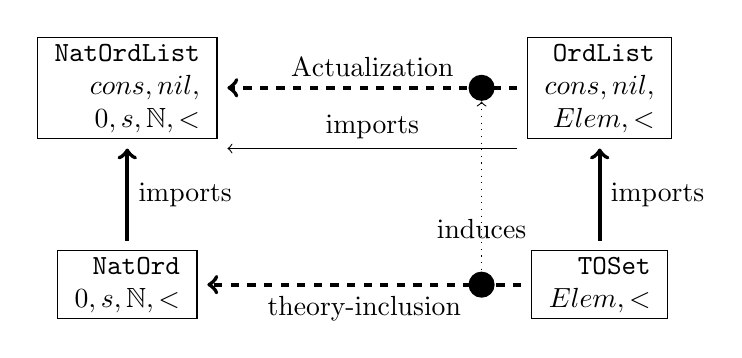
\begin{tikzpicture}  \node (natordlist) at (0,2.5) 
    {\begin{tabular}{|r|}\hline 
      {\tt{NatOrdList}}\\
      $cons, nil,$\\
      $0,s,{\mathbb{N}},<$\\\hline
    \end{tabular}};
  \node (natord) at (0,0) 
    {\begin{tabular}{|r|}\hline 
      {\tt{NatOrd}}\\
      $0,s,{\mathbb{N}},<$\\\hline
    \end{tabular}};
  \node (toset) at (6,0) 
    {\begin{tabular}{|r|}\hline 
      {\tt{TOSet}}\\
      $Elem,<$\\\hline
    \end{tabular}};
  \node (ordlist) at (6,2.5) 
    {\begin{tabular}{|r|}\hline 
      {\tt{OrdList}}\\
      $cons, nil,$\\
      $Elem,<$\\\hline
    \end{tabular}};
  \node[circle,fill] (act1) at (4.5,2.5) {};
  \node[circle,fill] (act2) at (4.5,0) {};
  \draw [->,line width=1.5pt] (natord) -- node[right]{imports} (natordlist);
  \draw [->,line width=1.5pt] (toset) -- node[right]{imports} (ordlist);
  \draw [->,dashed,line width=1.5pt] (toset) -- node[below]{theory-inclusion} (natord);
  \draw [->,dashed,line width=1.5pt] (ordlist) -- node[above]{Actualization} (natordlist);
  \draw [->] (ordlist.south west) -- node[above]{imports} (natordlist.south east);
  \draw [<-,dotted,near end] (act1) -- node{induces} (act2);
\end{tikzpicture}
\end{myfig}

In this example, we specify a theory {\snippet{OrdList}} of lists that is generic in the
elements (which is assumed to be a totally ordered set, since we want to talk about
ordered lists).  Then we will instantiate {\snippet{OrdList}} by applying it to the theory
{\snippet{NatOrd}} of natural numbers to obtain the intended theory {\snippet{NatOrdList}} of
lists of natural numbers.  The advantage of this approach is that we can re-use the
generic theory {\snippet{OrdList}} to apply it to other element theories like that of
``characters'' to obtain a theory of lists of characters.  In
{\twintoo{algebraic}{specification}} languages, we speak of {\defemph{parametric
    theories}}\twin{parametric}{theory}.  Here, the theory {\snippet{OrdList}} has a formal
{\indextoo{parameter}} (the theory {\snippet{TOSet}}) that can be instantiated later with
concrete values to get a {\twindef{theory}{instance}} (in our example the theory
{\snippet{NatOrdList}}).  We call this process theory {\defin{actualization}}.

We begin the extended example with the theories in the lower half of
{\myfigref{natlist:actualization}}.  The first is a (mock up of a) theory of totally
ordered sets. Then we build up the theory of natural numbers as an
{\twindef{abstract}{data type}} (see {\mychapref{adt}} for an introduction to abstract
data types in {\omdoc} and a more elaborate definition of $\mathbb N$). The
{\element{sortdef}} element posits that the set of natural numbers is given as the
{\defin{sort}} {\snippet{NatOrd}}, with the {\indextoo{constructor}s} {\snippet{zero}} and
{\snippet{succ}}. Intuitively, a sort represents an {\twintoo{inductively defined}{set}},
i.e. it contains exactly those objects that can be represented by the constructors only,
for instance the number three is represented as $s(s(s(0)))$, where $s$ stands for the
successor function (given as the constructor {\snippet{succ}}) and $0$ for the number zero
(represented by the constructor {\snippet{zero}}). Note that the theory {\snippet{nat}}
does not have any explicitly represented axioms. They are implicitly given by the abstract
data type structure, in our case, they correspond to the five Peano Axioms (see
{\myfigref{peano}}).  Finally, the {\element{argument}} elements also introduce one
partial inverse to the constructor functions per argument; in our case the
{\twintoo{predecessor}{function}}.

\begin{lstlisting}[mathescape,label=lst:nat-param,
  index={theory,symbol,definition,assertion}]
<theory xml:id="TOSet">                   
  <symbol name="set"/>
  <symbol name="ord"/>
  <axiom xml:id="toset"><CMP><xhtml:p>$ord$ is a  total order on $set$.</xhtml:p></CMP></axiom>
</theory>                               

<theory xml:id="nat">
  <adt>
    <sortdef name="Nat">
      <constructor name="zero"/>
      <constructor name="succ">
        <argument>
          <type><OMOBJ><OMS name="Nat" cd="nat"/></OMOBJ></type>
          <selector name="pred"/>
        </argument>
      </constructor>
    </sortdef>
  </adt>
</theory>

<theory xml:id="NatOrd">
  <imports from="#nat"/>
  <imports from="#TOSet"/>
  <symbol name="leq"/>
  <definition xml:id="leq.def" for="leq" type="implicit" 
              existence="#leq.ex" uniqueness="#leq.uniq">
    <FMP>$\allcdot{x}{0\leq x}\land\allcdot{x,y}{x\leq y\implies s(x)\leq s(y)}$</FMP>
  </definition>
  <assertion xml:id="leq.ex"><CMP><xhtml:p>$\leq$ exists.</xhtml:p></CMP></assertion>
  <assertion xml:id="leq.unique"><CMP><xhtml:p>$\leq$ is unique.</xhtml:p></CMP></assertion>
  <assertion xml:id="leq.TO"><CMP><xhtml:p>$\leq$ is a  total order on $Nat$.<xhtml:p></CMP></assertion>
</theory>                       
\end{lstlisting}

Finally we have extended the natural numbers by an ordering function $\leq$ (symbol
{\snippet{leq}}) which we show to be a total ordering function in assertion
{\snippet{leq.TO}}.  Note that to state the assertion, we had to import the notion of a
total ordering from theory {\snippet{TOSet}}. We can directly use this result to establish
a {\twindef{theory}{inclusion}} between {\snippet{TOSet}} as the
{\twindef{source}{theory}} and {\snippet{NatOrd}} as the {\twindef{target}{theory}}. A
{\twintoo{theory}{inclusion}} is a formula mapping between two theories, such that the
translations of all axioms in the {\twintoo{source}{theory}} are provable in the
{\twintoo{target}{theory}}. In our case, the mapping is given by the recursive function
given in the {\element{morphism}} element in {\mylstref{nat-ti}} that maps the respective
base sets and the ordering relations to each other. The {\element{obligation}} element
just states that translation of the only theory-constitutive
(see \mysubsecref{definitions}) element of the source theory (the axiom
{\snippet{toset}}) has been proven in the target theory, as witnessed
by the assertion {\snippet{leq.TO}}\footnote{Note that as always,
  {\omdoc} only cares about the structural aspects of this: The
  {\omdoc} model only insists that there is the statement of an
  assertion, whether the author chooses to prove it or indeed whether
  the statement is true at all is left to other levels of modeling.}.

\begin{lstlisting}[mathescape,label=lst:nat-ti,
  index={theory,symbol,definition,assertion}]
<theory-inclusion xml:id="elem-nat-incl" to="#NatOrd" from="#TOSet">
  <morphism xml:id="elem-nat" type="pattern">
    <requation>
      <OMOBJ><OMS cd="TOSet" name="set"/></OMOBJ>
      <OMOBJ><OMS cd="NatOrd" name="Nat"/></OMOBJ>
    </requation>
    <requation>
      <OMOBJ><OMS cd="TOSet" name="ord"/></OMOBJ>
      <OMOBJ><OMS cd="NatOrd" name="leq"/></OMOBJ>
    </requation>
  </morphism>
  <obligation induced-by="#toset" assertion="#leq.TO"/>
</theory-inclusion>
\end{lstlisting}

We continue our example by building a generic theory {\snippet{OrdList}} of ordered lists.
This is given as the abstract data type generated by the symbols {\snippet{cons}}
(construct a list from an element and a rest list) and {\snippet{nil}} (the empty list)
together with a defined symbol {\snippet{ordered}}: a predicate for ordered lists. Note
that this symbol cannot be given in the abstract data type, since it is not a constructor
symbol. Note that {\snippet{OrdList}} imports theory {\snippet{TOSet}} for the base set of
the lists and the ordering relation $\leq$.

\begin{lstlisting}[mathescape,label=ordered-list,
  index={theory,imports,adt,sortdef,constructor,argument,symbol,definition}]
<theory xml:id="OrdList">
  <imports from="#TOSet"/>
  <adt xml:id="list-adt">
    <sortdef name="lists">
      <constructor name="cons">
        <argument>
          <type><OMOBJ><OMS name="set" cd="TOSet"/></OMOBJ></type>
          <selector name="head"/>
        </argument>
        <argument>
          <type><OMOBJ><OMS name="lists" cd="OrdList"/></OMOBJ></type>
          <selector name="rest"/>
        </argument>
      </constructor>
      <constructor name="nil"/>
    </sortdef>
  </adt>

  <symbol name="ordered"/>
  <definition xml:id="ordered-def" for="ordered" type="informal">
    <CMP><xhtml:p>A list $l$ is called ordered, iff $head(l)\leq z$ for all elements $z\in rest(l)$ and
    $rest(l)$ is ordered.</xhtml:p></CMP>
  </definition>
</theory>
\end{lstlisting}

The theory {\snippet{NatOrdList}} of lists of natural numbers is built up by
importing from the theories {\snippet{NatOrd}} and {\snippet{OrdList}}. Note that the
attribute {\attribute{type}{imports}} of the {\element{imports}} element
{\snippet{nat-list.im-elt}} is set to {\attval{local}{type}{imports}}, since we
only want to import the local axioms of the theory {\snippet{OrdList}} and not the
whole theory {\snippet{OrdList}} (which would include the axioms from
{\snippet{TOSet}}; see {\mysecref{restricting-inference}} for a discussion). In
particular the symbols {\snippet{set}} and {\snippet{ord}} are not imported into
theory {\snippet{NatOrdList}}: the theory {\snippet{TOSet}} is considered as a
{\atwindef{formal}{parameter}{theory}}, which is actualized to the
{\atwindef{actual}{parameter}{theory}} with this construction.  The effect of the
actualization comes from the morphism {\snippet{elem-nat}} in the import of
{\snippet{OrdList}} that renames the symbol {\snippet{set}} (from theory
{\snippet{TOSet}}) with {\snippet{Nat}} (from theory {\snippet{NatOrd}}). The
actualization from {\snippet{OrdList}} to {\snippet{NatOrdList}} only makes sense, if
the parameter theory {\snippet{NatOrd}} also has a suitable ordering function.  This
can be ensured using the {\omdoc} {\element{inclusion}} element.

\begin{lstlisting}[mathescape,label=lst:nat-list,
  index={theory,imports,morphism,inclusion}]
<theory xml:id="NatOrdList">
  <imports xml:id="natordlist.im-natord" from="#NatOrd"/>
  <imports xml:id="natordlist.im-elt" from="#OrdList" type="local">
    <morphism base="#elem-nat"/>
  </imports>
  <inclusion via="elem-nat-incl"/>
</theory>
\end{lstlisting}
The benefit of this {\element{inclusion}} requirement is twofold: If the theory inclusion
from {\snippet{TOSet}} to {\snippet{NatOrd}} cannot be verified, then the theory
{\snippet{NatOrdList}} is considered to be undefined, and we can use the
{\twintoo{development}{graph}} techniques presented in {\mysecref{development-graphs}} to
obtain a theory inclusion from {\snippet{OrdList}} to {\snippet{NatOrdList}}: We first
establish an axiom inclusion from theory {\snippet{TOSet}} to {\snippet{NatOrdList}} by
observing that this is induced by composing the theory inclusion from {\snippet{TOSet}} to
{\snippet{NatOrd}} with the theory inclusion given by the {\element{imports}} from
{\snippet{NatOrd}} to {\snippet{NatOrdList}}. This gives us a
{\defin{decomposition}} situation: every theory that the source theory {\snippet{OrdList}}
inherits from has an axiom inclusion to the target theory {\snippet{NatOrdList}}, so the
local axioms of those theories are provable in the target theory. Since we have covered
all of the inherited ones, we actually have a theory inclusion from the source- to the
target theory.

\begin{lstlisting}[mathescape,label=lst:nat-list-inclusions,
  index={theory,imports,morphism,inclusion}]
<axiom-inclusion xml:id="toset-natordlist-incl" from="#TOSet" to="#NatOrdList">
  <morphism base="#elem-nat"/>
  <path-just local="#elem-nat-incl" globals="#natordlist.im-natord"/>
</axiom-inclusion>

<theory-inclusion from="#OrdList" to="#NatOrdList">
  <morphism base="#elem-nat"/>
  <decomposition links="#toset-natordlist-incl #elem-nat-incl"/>
</theory-inclusion>
\end{lstlisting}

This concludes our example, since we have seen that the theory {\snippet{OrdList}} is
indeed included in {\snippet{NatOrdList}} via renaming.

Note that with this construction we could simply extend the graph by actualizations for
other theories, e.g. to get {\twintoo{lists of}{character}s}, as long as we can prove
{\twintoo{theory}{inclusion}s} from {\snippet{TOSet}} to them.
\end{tchapter}

%%% Local Variables: 
%%% mode: latex
%%% TeX-master: "omdoc"
%%% End: 

% LocalWords:  natlist omcds TOSet adt sortdef succ nat peano mathescape lst ti
% LocalWords:  param ord toset pred NatOrd def uniq elem incl requation cd nats
% LocalWords:  OrdList im NatOrdList elt natordlist leq ns attr natord toset
% LocalWords:  toset CMP OMOBJ FMP toset natordlist natord natordlist toset

% LocalWords:  natordlist natord natordlist toset natordlist globals natordlist
% LocalWords:  natord toset natordlist toset toset toset natordlist natord
% LocalWords:  natordlist toset natordlist natordlist natord toset natordlist
% LocalWords:  toset toset toset natordlist natord natordlist toset natordlist
% LocalWords:  natordlist natord toset natordlist

%%%%%%%%%%%%%%%%%%%%%%%%%%%%%%%%%%%%%%%%%%%%%%%%%%%%%%%%%%%%%%%%%%%%%%%%%
% This file is part of the LaTeX sources of the OMDoc 1.3 specification
% Copyright (c) 2006 Michael Kohlhase
% This work is licensed by the Creative Commons Share-Alike license
% see http://creativecommons.org/licenses/by-sa/2.5/ for details
%%%%%%%%%%%%%%%%%%%%%%%%%%%%%%%%%%%%%%%%%%%%%%%%%%%%%%%%%%%%%%%%%%%%%%%%%

\begin{tchapter}[id=dg-elal]{A Development Graph for Elementary Algebra}
  We will now use the technique presented in the last chapter for the elementary algebraic
  hierarchy. {\Myfigref{rings-dg}} gives an overview of the situation. We will build up
  theories for semigroups, monoids, groups, and rings and a set of theory inclusions from
  these theories to themselves given by the converse of the operation.

\begin{myfig}{rings-dg}{A Development Graph for Elementary Algebra}
\fbox{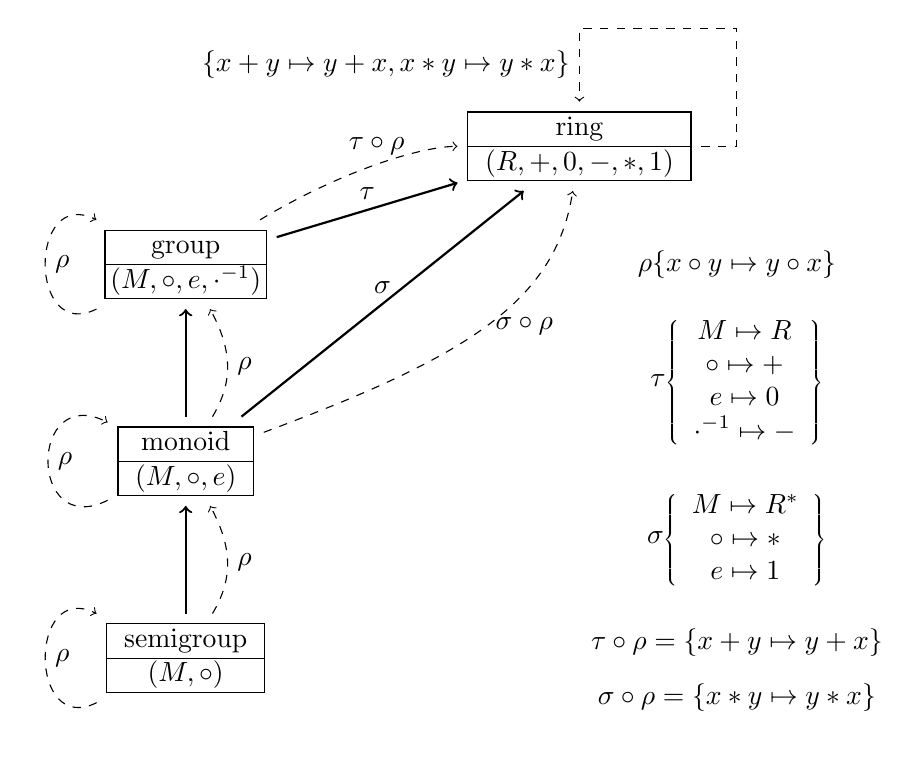
\begin{tikzpicture}
\node (sg) at (1,1)
   {\begin{tabular}{|c|}\hline 
       semigroup\\\hline 
       $(M,\circ)$\\\hline 
     \end{tabular}};
\node (mon) at (1,3.5)
    {\begin{tabular}{|c|}\hline 
      monoid\\\hline
      $(M,\circ,e)$\\\hline
    \end{tabular}};
\node (grp) at (1,6)
    {\begin{tabular}{|c|}\hline 
      group\\\hline
      \kern-1ex$(M,\circ,e,\cdot^{-1})\kern-1ex$\\\hline
    \end{tabular}};

\node (ring) at (6,7.5)
    {\begin{tabular}{|c|}\hline 
      ring\\\hline
      $(R,+,0,-,*,1)$\\\hline
    \end{tabular}};
\node (sigma) at (8,2.5)
    {$\sigma\deq\scriptscriptstyle\left\{\begin{array}{c}
      M\mapsto R^*\\\circ\mapsto *\\e\mapsto 1
    \end{array}\right\}$};
\node (tau) at (8,4.5)
    {$\tau\deq\scriptscriptstyle\left\{\begin{array}{c}
      M\mapsto R\\\circ\mapsto +\\e\mapsto 0\\\cdot^{-1}\mapsto -
    \end{array}\right\}$};

 \node (ts) at (8,6){$\rho\deq\{x\circ y\mapsto y\circ x\}$};
 \node (sr) at (8,.5){$\sigma\circ\rho=\{x*y\mapsto y*x\}$};
 \node (tr) at (8,1.2){$\tau\circ\rho=\{x+y\mapsto y+x\}$};
 \draw [->,thick](sg) -- (mon);
 \draw [->,thick](mon) -- (grp);
 \draw [->,thick](mon) -- node[above]{$\sigma$} (ring);
 \draw [->,thick](grp) -- node[above]{$\tau$} (ring);p
 \draw [->,dashed](mon) .. controls (4.5,4.8) and (5.7,5.5) .. 
     node[right]{$\sigma\circ\rho$} (ring);
 \draw [->,dashed](grp) .. controls (3,7.2) and (4,7.5) .. 
     node[above]{$\tau\circ\rho$} (ring);
 \draw [->,dashed] (sg) .. controls (-1,0) and (-1,2) .. 
     node[right]{$\rho$}(sg);
 \draw [->,dashed] (mon) .. controls (-1,2.5) and (-1,4.5) .. 
     node[right]{$\rho$}(mon);
 \draw [->,dashed] (grp) .. controls (-1,5) and (-1,7) .. 
     node[right]{$\rho$}(grp);
 \draw [->,dashed] (sg) .. controls (1.6,2) and (1.6,2.4) .. 
     node[right]{$\rho$}(mon);
 \draw [->,dashed] (mon) .. controls (1.6,4.5) and (1.6,4.9) .. 
     node[right]{$\rho$}(grp);
 \draw [->,dashed] (ring) -- (8,7.5) -- (8,9) -- (6,9) --
     node[left]{$\{x+y\mapsto y+x,x*y\mapsto y*x\}$} (ring);
\end{tikzpicture}}
\end{myfig}

We start off with the theory for {\emin{semigroup}s}. It introduces two symbols, the base
set $M$ and the operation $\circ$ on $M$ together with two axioms that state that $M$ is
closed under $\circ$ and that $\circ$ is associative on $M$. We have a structural theory
inclusion from this theory to itself that uses the fact that $M$ together with the
converse $\sigma(\circ)$ of $\circ$ is also a semigroup: the obligation for the axioms can
be justified by themselves (for the closure axiom we have
$\sigma(\allcdot{x,y\in{M}}{x\circ y\in{M}})=\allcdot{y,x\in{M}}{x\circ y\in{M}}$, which
is logically equivalent to the axiom.)

\begin{lstlisting}[mathescape,
  index={theory-inclusion,morphism,requation}]
<theory xml:id="semigroup">
  <symbol name="base-set"/>
  <presentation for="#base-set"><use format="default">$M$</use></presentation>
  <symbol name="op"/>
  <presentation for="#op"><use format="default">$\circ$</use></presentation>
  <axiom xml:id="closed.ax"><FMP>$\allcdot{x,y\in{M}}{x\circ y\in{M}}$</FMP></axiom>
  <axiom xml:id="assoc.ax">
    <FMP>$\allcdot{x,y,z\in{M}}{(x\circ y)\circ z=x\circ(y\circ z)}$</FMP>
  </axiom>
</theory>

<theory-inclusion xml:id="sg-conv-sg" from="#semigroup" to="#semigroup">
  <morphism xml:id="sg-conv-sg.morphism">
    <requation>$X\circ Y\leadsto Y\circ X$</requation>
  </morphism>
  <obligation assertion="conv.closed" induced-by="#closed.ax"/>
  <obligation assertion="#assoc.ax" induced-by="#assoc.ax"/>
</theory-inclusion>
\end{lstlisting}
The theory of {\emin{monoid}s} is constructed as an extension of the theory of semigroups
with the additional unit axiom, which states that there is an element that acts as a
(right) unit for $\circ$. As always, we state that there is a unique such unit, which
allows us to define a new symbol $e$ using the
{\atwintoo{definite}{description}{operator}} $\thatcdot{x}{}$: If there is a unique $x$,
such that $\bA$ is true, then the construction $\thatcdot{x}\bA$ evaluates to $x$, and is
undefined otherwise. We also prove that this $e$ also acts as a left unit for $\circ$.

\begin{lstlisting}[mathescape]
<theory xml:id="monoid">
  <imports xml:id="sg2mon" from="#semigroup"/>
  <axiom xml:id="unit.ax"><FMP>$\excdot{x\in{M}}{\allcdot{y\in{M}}{y\circ x=y}}$</FMP></axiom>
  <assertion xml:id="unit.unique"><FMP>$\exucdot{x\in{M}}{\allcdot{y\in{M}}{y\circ x=y}}$</FMP></assertion>
  <symbol name="unit" xml:id=''unit''/>
  <presentation for="#unit"><use format="default">e</use></presentation>
  <definition xml:id="unit.def" for="unit" type="simple" existence="#unit.unique">
    $\thatcdot{x\in{M}}{\allcdot{y\in{M}}{y\circ x=y}}$
  </definition>
  <assertion xml:id="left.unit"><FMP>$\allcdot{x\in{M}}{e\circ x=x}$</FMP></assertion>
  <symbol name="setstar" xml:id=''setstar''/>
  <presentation for="#setstar" fixity="postfix">
    <use format="default">$^*$</use>
  </presentation>
  <definition xml:id="ss.def" for="setstar" type="implicit">
    $\allcdot{S\subseteq{M}}{S^*=S\backslash\set{e}}$
  </definition>
</theory>
\end{lstlisting}

Building on this, we first establish an axiom-selfinclusion from the theory of
monoids to itself. We can make this into a {\twintoo{theory}{selfinclusion}} using
the theory-selfinclusion for semigroups as the local part of a path justification
(recall that theory inclusions are axiom inclusions by construction) and the
definitional theory inclusion induced by the import from semigroups to monoids as
the global path.
\begin{lstlisting}[mathescape,index={axiom-inclusion,theory-inclusion,morphism,obligation}]
<axiom-inclusion  xml:id="mon-conv-mon.local" from="#monoid" to="#monoid">
  <morphism base="#sg-conv-sg.morphism"/>
  <obligation assertion="#left.unit" induced-by="#unit.ax"/>
</axiom-inclusion>

<axiom-inclusion xml:id="sg-conv-mon" from="#semigroup" to="#monoid">
  <morphism base="#sg-conv-sg.morphism"/>
  <path-just local="#sg-conv-sg" globals="#sg2mon"/>
</axiom-inclusion>
<theory-inclusion xml:id="mon-conv-mon.global" from="#monoid" to="#monoid">
  <morphism base="#sg-conv-sg.morphism"/>
  <decomposition links="#sg-conv-sg #sg-conv-mon"/>
</theory-inclusion>
\end{lstlisting}
Note that all of these axiom inclusions have the same morphism (denoted by $\rho$
in {\myfigref{rings-dg}}), in {\omdoc} we can share this structure using the
{\attribute{base}{morphism}} on the {\element{morphism}} element. This normally
points to a morphism that is the base for extension, but if the
{\element{morphism}} element is empty, then this just means that the morphisms are
identical. 

For groups, the situation is very similar: We first build a theory of groups by
adding an axiom claiming the existence of inverses and constructing a new function
$\cdot^{-1}$ from that via a definite description. 

\begin{lstlisting}[mathescape]
<theory xml:id="group">
  <imports xml:id="mon2grp" from="#monoid"/>
  <axiom xml:id="inv.ax"><FMP>$\allcdot{x\in{M}}{\excdot{y\in{M}}{x\circ y=e}}$</FMP></axiom>
  <symbol name="inv" xml:id=''inv''/>
  <presentation for="#inv" role="applied">
    <use format="default" lbrack="" rbrack="" fixity="postfix">$^{-1}$</use>
  </presentation>
  <definition xml:id="inv.def" for="inv" type="pattern">
    <requation>$x^{-1}\leadsto\thatcdot{y}x\circ y=e$</value></requation>
  </definition>
  <assertion xml:id="conv.inv"><FMP>$\allcdot{x\in{M}}{\excdot{y\in{M}}{y\circ x=e}}$</FMP></assertion>
</theory>
\end{lstlisting}

Again, we have to establish a couple of axiom inclusions to justify the theory
inclusion of interest. Note that we have one more than in the case for monoids,
since we are one level higher in the inheritance structure, also, the local chains
are one element longer.
\begin{lstlisting}[mathescape,index={axiom-inclusion,theory-inclusion}]
<axiom-inclusion xml:id="grp-conv-grp.local" from="#group" to="#group">
  <morphism base="#sg-conv-sg.morphism"/>
  <obligation assertion="conv.inv" induced-by="#inv.ax"/>
</axiom-inclusion>
<axiom-inclusion xml:id="sg-conv-grp" from="#semigroup" to="#group">
  <morphism base="#sg-conv-sg.morphism"/>
  <path-just local="#sg-conv-sg" globals="#mon2grp #sg2mon"/>
</axiom-inclusion>
<axiom-inclusion xml:id="mon-conv-grp" from="#monoid" to="#group">
  <morphism base="#sg-conv-sg.morphism"/>
  <path-just local="#mon-conv-mon.local" globals="#mon2grp"/>
</axiom-inclusion>
<theory-inclusion xml:id="grp-conv-grp" from="#group" to="#group">
  <morphism base="#sg-conv-sg.morphism"/>
  <decomposition links="#sg-conv-grp #mon-conv-grp #grp-conv-grp.local"/>
</theory-inclusion>
\end{lstlisting}
Finally, we extend the whole setup to a theory of rings. Note that we have a dual import
from {\snippet{group}} and {\snippet{monoid}} with different morphisms (they are
represented by $\sigma$ and $\tau$ in {\myfigref{rings-dg}}). These rename all of the
imported symbols apart (interpreting them as additive and multiplicative) except of the
punctuated set constructor $\cdot^*$, which is imported from the additive group structure
only. We avoid a name clash with the operator that would have been imported from the
multiplicative structure by specifying that this is not imported using the
{\attribute{hiding}{morphism}} on the {\element{morphism}} in the respective
{\element{imports}} element\footnote{An alternative (probably better) to this would have
  been to explicitly include the operators in the morphisms, creating new operators for
  them in the theory of {\snippet{rings}}.  But the present construction allows us to
  exemplify the {\attribute{hiding}{morphism}}, which has not been covered in an example
  otherwise.}.

\begin{lstlisting}[mathescape,index={theory,imports}]
<theory xml:id="ring"> 
  <symbol name="R" xml:id=''R''/>
  <presentation for="#R"><use format="default">R</use></presentation>
  <symbol name="zero"/>
  <presentation for="#zero"><use format="default">0</use></presentation>
 <symbol name="plus"/>
 <presentation for="#plus" role="applied">
    <use format="default">+</use>
  </presentation>
 <symbol name="negative"/>
 <presentation for="#negative" role="applied">
    <use format="default">-</use>
  </presentation>
 <symbol name="times"/>
  <presentation for="#times" role="applied">
    <use format="default">*</use>
  </presentation>
  <symbol name="one"/> 
  <presentation for="#one"><use format="default">1</use></presentation>
  <imports xml:id="add.import" from="#group"> 
    <morphism>$M\mapsto R,x\circ y\mapsto x*y, e\mapsto 1,\cdot^{-1}\mapsto -$</morphism> 
  </imports> 
  <imports xml:id="mult.import" from="#monoid"> 
    <morphism hiding="setstar">$M\mapsto M^*,x\circ y\mapsto x*y, e\mapsto 1$</morphism> 
  </imports> 
  <axiom xml:id="dist.ax"><FMP>$x*(y+z)=(x*y)+(x*z)$</FMP></axiom> 
  <assertion xml:id="dist.conv"><FMP>$(z+y)*x=(z*x)+(y*x)$</FMP></assertion>
</theory>
\end{lstlisting}

Again, we have to establish some axiom inclusions to justify the
{\twintoo{theory}{selfinclusion}} we are after in the example. Note that in the
rings case, things are more complicated, since we have a dual import in the theory
of {\snippet{rings}}. Let us first establish the additive part. 
 
\begin{lstlisting}[mathescape,index={axiom-inclusion,theory-inclusion}]
<axiom-inclusion xml:id="sg-conv-rg.add" from="#semigroup" to="#ring">
  <morphism base="#sg-conv-sg.morphism #add.import"/>
  <path-just local="#sg-conv-sg" globals="#sg2mon #mon2grp #add.import "/>
</axiom-inclusion>
<axiom-inclusion xml:id="mon-conv-rg.add" from="#monoid" to="#group">
  <morphism base="#sg-conv-sg.morphism #add.import"/>
  <path-just local="#mon-conv-mon.local" globals="#mon2grp #add.import"/>
</axiom-inclusion>
<axiom-inclusion xml:id="grp-conv-rg.add" from="#group" to="#group">
  <morphism base="#sg-conv-sg.morphism #add.import"/>
  <path-just local="#grp-conv-grp.local" globals="#add.import"/>
</axiom-inclusion>
\end{lstlisting}
The multiplicative part is totally analogous, we will elide it to conserve space.
Using both parts, we can finally get to the local axiom self-inclusion and extend
it to the intended theory inclusion justified by the axiom inclusions established
above.
\begin{lstlisting}[mathescape,index={axiom-inclusion,theory-inclusion}]
<axiom-inclusion xml:id="rg-conv-rg.local" from="#ring" to="#ring">
  <morphism xml:id="rg-conv-rg.morphism">$x+y\mapsto y+x,x*y\mapsto y*x$</morphism>
  <obligation assertion="#dist.conv" induced-by="#dist.ax"/>
</axiom-inclusion>  
<theory-inclusion xml:id="rg-conv-rg" from="#ring" to="#ring">
  <morphism base="#rg-conv-rg.morphism"/>
  <decomposition links="#rg-conv-rg.local 
                        #sg-conv-rg.add  #mon-conv-rg.add  #grp-conv-rg.add
                        #sg-conv-rg.mult #mon-conv-rg.mult #grp-conv-rg.mult"/>
</theory-inclusion>  
\end{lstlisting}
This concludes our example. It could be extended to higher constructs in algebra
like fields, magmas, or vector spaces easily enough using the same methods, but
we have seen the key features already.
\end{tchapter}

%%% Local Variables: 
%%% mode: latex
%%% TeX-master: "omdoc"
%%% End: 
 

% LocalWords:  dg elal sg mon grp linewidth arcangle angleA angleB mathescape
% LocalWords:  requation conv def uniq setstar ss selfinclusion lbrack ts
% LocalWords:  rbrack mult dist sr tr FMP globals inv rg

%%%%%%%%%%%%%%%%%%%%%%%%%%%%%%%%%%%%%%%%%%%%%%%%%%%%%%%%%%%%%%%%%%%%%%%%%
% This file is part of the LaTeX sources of the OMDoc 1.3 specification
% Copyright (c) 2006 Michael Kohlhase
% This work is licensed by the Creative Commons Share-Alike license
% see http://creativecommons.org/licenses/by-sa/2.5/ for details
\svnInfo $Id: courseware.tex 9251 2012-07-23 10:29:02Z kohlhase $
\svnKeyword $HeadURL: https://svn.omdoc.org/repos/omdoc/branches/omdoc-1.3/doc/spec/courseware.tex $
%%%%%%%%%%%%%%%%%%%%%%%%%%%%%%%%%%%%%%%%%%%%%%%%%%%%%%%%%%%%%%%%%%%%%%%%%

\begin{tchapter}[id=courseware]{Courseware and the Narrative/Content Distinction}

In this chapter we will look at another type of mathematical document:
{\indextoo{courseware}}; in this particular case a piece from an introductory
course ``{\indextoo{Fundamentals of Computer Science}}\twin{computer}{science}''
(Course 15-211 at {\indextoo{Carnegie Mellon University}}). The {\omdoc} documents
produced from such courseware can be used as input documents for {\activemath}
(see {\mysecref{activemath}}) and can be produced e.g. by {\cpoint} (see
{\mysecref{cpoint}}).

\begin{myfig}{15-211}{Three slides from 15-211}
  \fbox{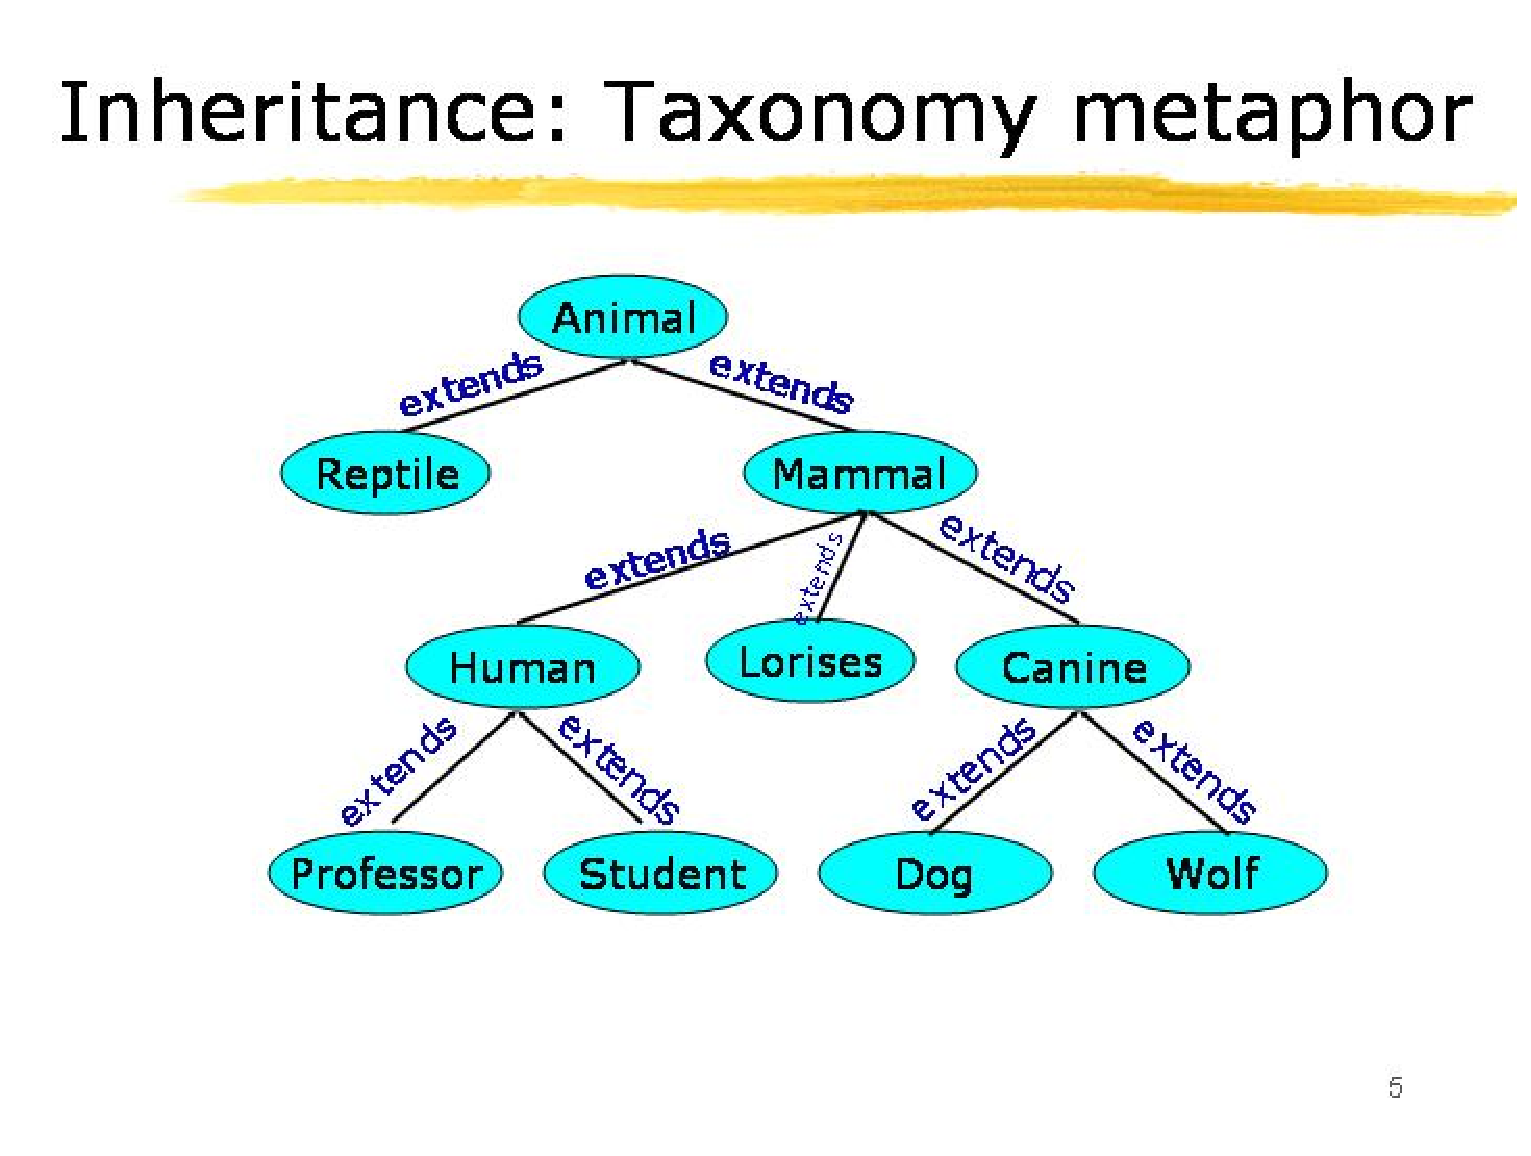
\includegraphics[width=5.2cm]{figures/slide-847}}\quad
  \fbox{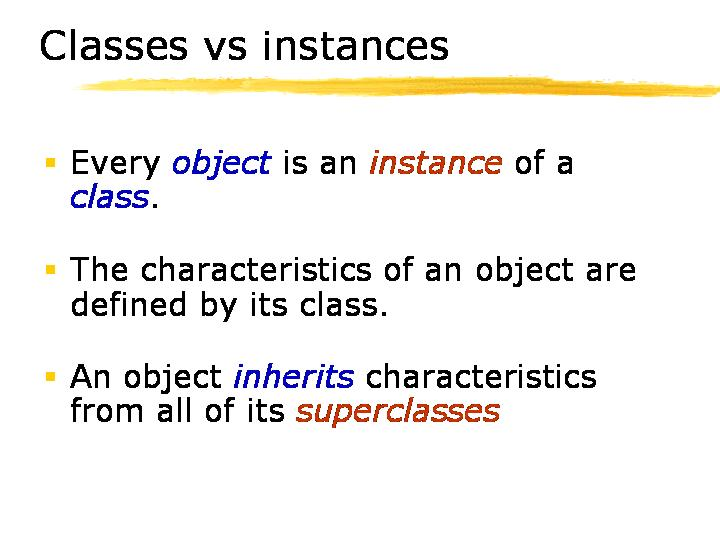
\includegraphics[width=5.2cm]{figures/slide-862}}\\[1ex]
  \fbox{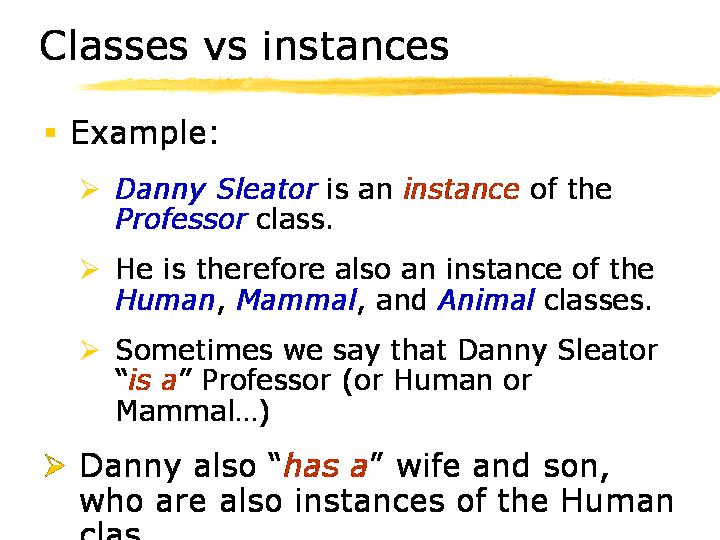
\includegraphics[width=5.2cm]{figures/slide-863}}\quad
  \fbox{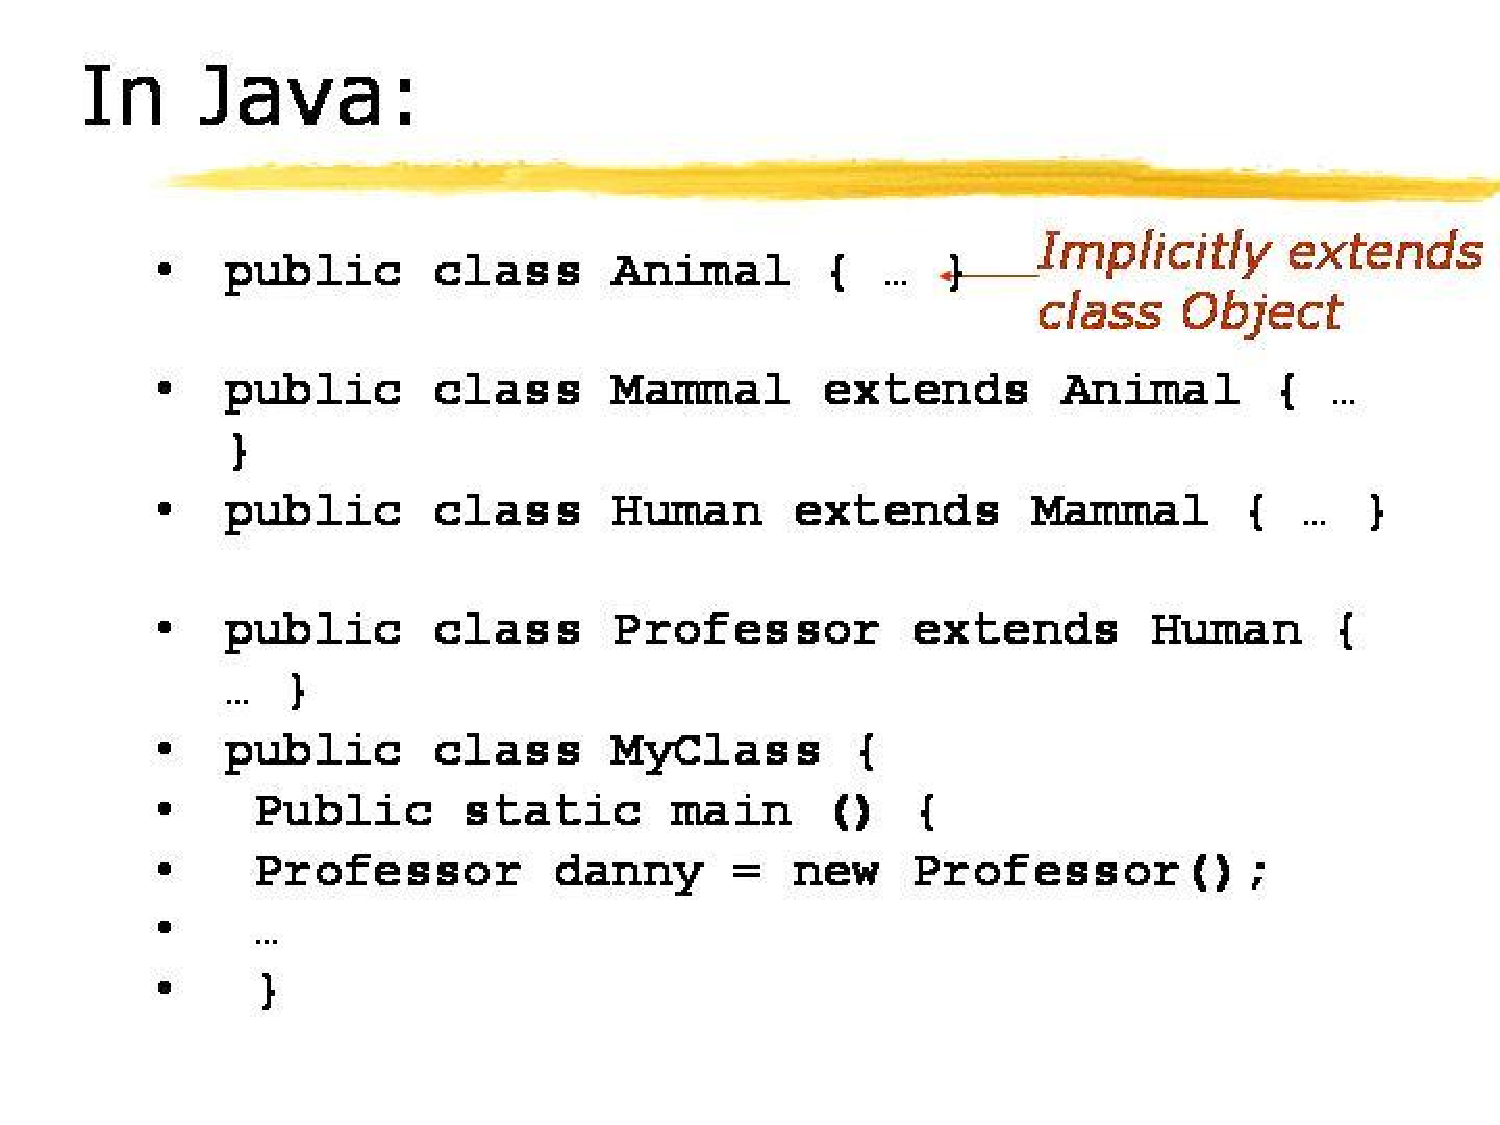
\includegraphics[width=5.2cm]{figures/slide-864}}
\end{myfig}

We have chosen a fragment that is relatively far from conventional mathematical
texts to present the possibility of semantic markup in {\omdoc} even under such
circumstances.  We will highlight the use of {\omdoc} theories\index{theory} for
such an application. Furthermore, we will take seriously the difference between
marking up the knowledge (implicitly) contained in the {\indextoo{slide}s} and the
{\indextoo{slide presentation}}\index{presentation!slides} as a structured
document. As a consequence, we will capture the slides in {\emph{two}} documents:

\begin{itemize}
\item a {\emph{knowledge-centered\twin{knowledge-centered}{document} document}}, which contains
  the knowledge conveyed in the course organized by its inherent logical structure
\item a {\emph{narrative-structured\twin{narrative-structured}{document} document}}
  references the knowledge items and adds rhetorical and didactic structure of a
  slide presentation.
\end{itemize}
This separation of concerns into two documents is good practice in marking up mathematical
texts: It allows to make explicit the structure inherent in the respective domain and at
the same time the structure of the presentation that is driven by didactic needs. We
call knowledge-structured documents {\twindef{content}{OMDoc}s} and narrative-structured
ones {\twindef{narrative}{OMDoc}s}.  The separation also simplifies management of academic
content\twin{content}{management}: The content {\omdoc} of course will usually be shared
between individual installments of the course, it will be added to,
{\indextoo{correct}ed}, {\indextoo{cross-reference}d}, and kept up to date by different
authors. It will eventually embody the institutional memory of an organization like a
university or a group of teachers.  The accompanying narrative {\omdoc}s will capture the
different didactic tastes and approaches by individual teachers and can be adapted for the
installments of the course. Since the narrative {\omdoc}s are relatively light-weight
structures (they are largely void of original content, which is referenced from the
content {\omdoc}) constructing or tailoring a course to the needs of the particular
audience becomes a simpler endeavor of choosing a path through a large repository of
marked up knowledge embodied in the content {\omdoc} rather than
re-authoring\footnote{Since much of the re-authoring is done by copy and paste in the
  current model, it propagates errors in the course materials rather than corrections.}
the content with a new slant.

Let us look at the four slides in {\myfigref{15-211}}. The first
{\indextoo{slide}} shows a graphic of a simple {\indextoo{taxonomy}} of
{\indextoo{animal}s}, the second one introduces first concepts from
{\twintoo{object-oriented}{programming}}, the
third one gives examples for these interpreting the class hierarchy introduced in
the first slide, finally the fourth slide gives code concrete snippets as examples
for the concepts introduced in the first three ones.

We will first discuss content {\omdoc} and then the narrative {\omdoc} in
{\mysecref{narrative-structured}}.

\begin{tsection}[id=knowledge-centered]{A Knowledge-Centered View}
  
  In this section, we will take a look at how we can make the knowledge that is contained
  in the slides in {\myfigref{15-211}} and its structure explicit so that a
  {\twintoo{knowledge}{management}} system like {\mbase} (see {\mysecref{mbase}}) or
  {\twintoo{knowledge}{presentation}} system like {\activemath} (see
  {\mysecref{activemath}}) can take advantage of it. We will restrict ourselves to
  knowledge that is explicitly represented in the slides in some form, even though the
  knowledge document would probably acquire more and more knowledge in the form of
  examples, graphics, variant definitions, and explanatory text as it is re-used in many
  courses.

The first slide introduces a theory, which we call {\snippet{animals-tax}}; see
{\mylstref{ann-tax}}.  It declares {\twintoo{primitive}{symbol}s} for all the
{\indextoo{concept}s}\footnote{The type information in the symbols is not strictly
  included in the slides, but may represent the fact that the instructor said that
  the ovals represent ``concepts''.}  (the ovals), and for all the links
introduced in the graphic it has {\element{axiom}} elements stating that the
parent node in the {\indextoo{tree}} extends the child node. The axiom uses the
symbol for {\twintoo{concept}{extension}} from a theory {\snippet{kr}} for
{\twintoo{knowledge}{representation}} which we import in the theory and which we
assume in the background materials for the course.

\begin{lstlisting}[label=lst:ann-tax,mathescape,
    caption={The {\omdoc} Representation for Slide 1 from {\myfigref{15-211}}},
    index={theory,axiom,symbol,CMP,FMP,OMA,OMOBJ,OMS,private,data}]
<theory xml:id="animals-tax">
  <imports xml:id="tax_imports_taxonomy" from="#taxonomies"/>
  <imports xml:id="tax_imports_kr" from="#kr"/>
  <symbol name="human">
    <type system="stlc"><OMOBJ><OMS cd="kr" name="concept"/></OMOBJ></type>
  </symbol>
  <symbol name="mammal">
    <type system="stlc"><OMOBJ><OMS cd="kr" name="concept"/></OMOBJ></type>
  </symbol>
  $\ldots$
  <axiom xml:id="mammal-ext-human">
    <CMP><xhtml:p>Humans are Animals.</xhtml:p></CMP>
    <FMP>
      <OMOBJ>
        <OMA><OMS cd="kr" name="extends"/>
          <OMS cd="animal-taxonomy" name="mammal"/>
          <OMS cd="animal-taxonomy" name="human"/>
        </OMA>
      </OMOBJ>
    </FMP>
  </axiom>
  $\ldots$
</theory>

<private xml:id="tax-image" for="#animals-tax" reformulates="#animals-tax">
  <data format="image/jpeg" href="animals-taxonomy.jpg"/>
  <data format="application/postscript" href="animals-taxonomy.ps"/>
</private>
\end{lstlisting}
The {\element{private}} element contains the reference to the image in various
formats. Its {\attribute{reformulates}{private}} attribute hints that the image
contained in this element can be used to illustrate the theory above (in fact, it
will be the only thing used from this theory in the narrative {\omdoc} in
{\mylstref{ann-narrative}}.)

The second slide introduces some basic concepts in object oriented programming.  These
give rise to the five {\twintoo{primitive}{symbol}s} of the theory. Note that this theory
is basic, it does not import any other. The three text blocks are marked up as axioms,
using the attribute {\attribute{for}{axiom}} to specify the symbols involved in these
axioms. The value of the {\attribute{for}{axiom}} attribute is a whitespace-separated list
of {\twintoo{URI}{reference}s} to {\element{symbol}} elements.

\begin{lstlisting}[label=lst:ann-oo,
    caption={The {\omdoc} Representation for Slide 2 from {\myfigref{15-211}}},
    index={theory,axiom,symbol,CMP,FMP,OMA,OMOBJ,OMS}]
<theory xml:id="cvi">
  <symbol name="object" xml:id="cvi.object"/>
  <symbol name="instance" xml:id="cvi.instance"/>
  <symbol name="class" xml:id="cvi.class"/>
  <symbol name="inherits" xml:id="cvi.inherits"/>
  <symbol name="superclass" xml:id="cvi.superclass"/>

  <axiom xml:id="ax1" for="object instance class">
    <CMP>
      <xhtml:p>
        Every <xhtml:span style="font-style:italic;color:blue">object</xhtml:span>
        is an <xhtml:span style="font-style:italic;color:red">instance</xhtml:span> 
        of a <xhtml:span style="font-style:italic;color:blue">class</xhtml:span>.
     </xhtml:p>
    </CMP>
  </axiom>

  <axiom xml:id="ax2" for="class">
    <CMP><xhtml:p>The characteristics of an object are defined by its class.</xhtml:p></CMP>
  </axiom>

  <axiom xml:id="ax3" for="inherits superclass">
    <CMP><xhtml:p>An object <xhtml:span style="font-style:italic;color:blue">inherits</xhtml:span>
      characteristics from all of its 
      <xhtml:span style="font-style:italic;color:red">superclasses</xhtml:span>.</xhtml:p></CMP>
   </axiom>
</theory>
\end{lstlisting}

For the third slide it is not entirely obvious which of the {\omdoc} elements we want to
use for markup. The intention of the slide is obviously to give some {\indextoo{example}s}
for the concepts introduced in the second slide in terms of the taxonomy presented in the
first slide in {\myfigref{15-211}}. However, the {\omdoc} {\element{example}} element
seems to be too specific to directly capture the contents (see
p.~\pageref{eldef:example}). What is immediately obvious is that the slide introduces some
new knowledge and symbols, so we have to have a separate theory for this slide. The first
item in the list headed by the word Example is a piece of new knowledge, it is therefore
not an example at all, but an axiom\footnote{We could say that the function of being an
  example has moved up from mathematical statements to mathematical theories; we will not
  pursue this here.}. The second item in the list is a statement that can be deduced from
the knowledge we already have at our disposal from theories {\snippet{animals-tax}}
and {\snippet{cvi}}.  Therefore, the new theory {\snippet{cvi-examples}} in
{\mylstref{ann-cvi-ex}} imports these two. Furthermore, it introduces the new symbol
{\snippet{danny}} for ``Danny Sleator'' which is clarified in the {\element{axiom}}
element with {\snippet{xml:id="ax1"}}. Finally, the third item in the list does not have
the function of an example either, it introduces a new concept, the ``is a''
relation{\index{isa@``is a'' relation}}\index{relation!``is a''}\footnote{Actually, this
  text block introduces a new concept ``by reference to examples'', which is not a formal
  definition at all. We will neglect this for the moment.}.  So we arrive at the theory in
{\mylstref{ann-cvi-ex}}.  Note that this markup treats the last text block on the third
slide without semantic function in the theory -- it points out that there are other
relations among humans -- and leaves it for the narrative-structured {\omdoc} in
{\mysecref{narrative-structured}}\footnote{Of course this design decision is debatable,
  and depends on the intuitions of the author.  We have mainly treated the text this way
  to show the possibilities of semantic markup}.

\begin{lstlisting}[label=lst:ann-cvi-ex,
    caption={The {\omdoc} Representation for Slide 3 from {\myfigref{15-211}}},
    index={theory,imports,axiom,symbol,assertion,definition,CMP}]
<theory xml:id="cvi-examples">
  <imports from="#animals-tax"/><imports from="#cvi"/>

  <symbol name="danny" xml:id="cvi-examples.danny">
    <metadata><dc:description>Danny Sleator</dc:description></metadata>
  </symbol>

  <axiom xml:id="danny-professor" for="class instance danny">
    <CMP>
      <xhtml:p>
        <xhtml:span style="font-style:italic;color:blue">Danny Sleator</xhtml:span>
       is an <xhtml:span style="font-style:italic;color:red">instance</xhtml:span> 
       of the <xhtml:span style="font-style:italic;color:blue">Professor</xhtml:span> 
       class.
      </xhtml:p>
    </CMP>
  </axiom>

  <assertion xml:id="dannys-classes" type="theorem">
    <CMP>
      <xhtml:p>
        He is therefore also an instance of the 
        <xhtml:span style="font-style:italic;color:blue">Human</xhtml:span>, 
        <xhtml:span style="font-style:italic;color:blue">Mammal</xhtml:span>, 
        <xhtml:span style="font-style:italic;color:blue">Animal</xhtml:span> classes.
      </xhtml:p>
    </CMP>
  </assertion>

  <symbol name="is_a" scope="global">
    <metadata><dc:subject>'is a' relation</dc:subject></metadata>
  </symbol>

  <definition xml:id="is_a-def" for="is_a" type="informal">
     <CMP>
        <xhtml:p>Sometimes we say that Danny Sleator 
         &#x201C;<xhtml:span style="font-style:italic;color:red">is a</xhtml:span>&#x201D; 
         Professor (or Human or Mammal&#x2026;)
       </xhtml:p>
     </CMP>
  </definition>
</theory>
\end{lstlisting}

An alternative, more semantic way to mark up the {\element{assertion}} element in the
theory above would be to split it into multiple {\element{assertion}} and
{\element{example}} elements, as in {\mylstref{var-cvi-ex}}, where we have also added
formal content. We have split the {\indextoo{assertion}} {\snippet{dannys-classes}} into
three --- we have only shown one of them in {\mylstref{var-cvi-ex}} --- separate
assertions about class instances, and used them to justify the explicit examples. These
are given as {\omdoc} {\element{example}} elements. The {\attribute{for}{example}}
attribute of an {\element{example}} element points to the concepts that are exemplified
here (in this case the symbols for the {\indextoo{concept}s} ``instance'', ``class'' from
the theory {\snippet{cvi}} and the concept ``mammal'' from the animal taxonomy). The
{\attribute{type}{example}} specifies that this is not a {\indextoo{counter-example}}, and
the {\attribute{assertion}{example}} points to the justifying assertion. In this
particular case, the reasoning behind the example is pretty straightforward (therefore it
has been omitted in the slides), but we will make it explicit to show the mechanisms
involved. The {\element{assertion}} element just re-states the assertion implicit in the
example, we refrain from giving the formal statement in an {\element{FMP}} child here to
save space. The {\attribute{just-by}{assertion}} can be used to point to set of proofs for
this assertion, in this case only the one given in {\mylstref{var-cvi-ex}}. We use the
{\omdoc} {\element{proof}} element to mark up this proof.  It contains a series of
{\element{derive}} proof steps. In our case, the argument is very simple, we can see that
Danny Sleator is an instance of the human class, using the knowledge that
\begin{enumerate}
\item Danny is a professor (from the axiom in the {\snippet{cvi-examples}} theory)
\item An object inherits all the characteristics from its superclasses (from the
  axiom {\snippet{ax3}} in the {\snippet{cvi}} theory)
\item The human class is a superclass of the professor class (from the axiom
  {\snippet{human-extends-professor}} in the {\snippet{animal-taxonomy}} theory).
\end{enumerate}
The use of this knowledge in the proof step is made explicit by the
{\element{premise}} children of the {\element{derive}} element.

The information in the proof could for instance be used to generate very detailed
explanations for students who need help understanding the content of the original
slides in {\myfigref{15-211}}.


\begin{lstlisting}[label=lst:var-cvi-ex,mathescape,
    caption={An Alternative Representation Using {\element{example}} Elements},
    index={example,proof,assertion,derive,premise}]
$\ldots$
<example xml:id="danny-mammal" type="for" assertion="#dannys-mammal-thm"
         for="#cvi.instance #cvi.class #animal-taxonomy.mammal">
  <CMP><xhtml:p>Danny Sleator is an instance of the 
    <xhtml:span style="font-style:italic;color:blue">Mammal</xhtml:span> class. 
  <xhtml:p></CMP>
  <OMOBJ><OMS cd="cvi-examples" name="danny"/></OMOBJ>
</example>

<assertion xml:id="dannys-mammal-thm" type="theorem" proofs="#danny-mammal-pf">
  <CMP><xhtml:p>Danny Sleator is an instance of the Human class.</xhtml:p></CMP>
</assertion>

<proof xml:id="danny-human-pf" for="#dannys-mammal-thm">
  <derive xml:id="d1">
    <CMP><xhtml:p>Danny Sleator is an instance of the human class.</xhtml:p></CMP>
    <method>
      <premise xref="#danny-professor"/>
      <premise xref="#cvi.ax3"/>
      <premise xref="#animal-tax.human-extends-professor"/>
    </method>
  </derive>
  <derive xml:id="concl">
    <CMP><xhtml:p>Therefore he is an instance of the human class.</xhtml:p></CMP>
    <method>
      <premise xref="#d1"/>
      <premise xref="#cvi.ax3"/>
      <premise xref="#animal-tax.mammal-extends-human"/>
    </method>
  </derive>
</proof>
$\ldots$
\end{lstlisting}

The last slide contains a set of {\indextoo{Java}} {\twintoo{code}{fragment}s} that are
related to the material before.  We have marked them up in the {\element{code}} elements
in {\mylstref{cvi-code}}. The actual code is encapsulated in a {\element{data}} element,
whose {\attribute{format}{data}} specifies the format the data is in. The program text is
encapsulated in a {\indextoo{CDATA}} section to suspend the {\xml} {\indextoo{parser}}
(there might be characters like {\snippet{<}} or {\snippet{\&}} in there which offend it).
The {\element{code}} elements allow to document the {\indextoo{input}},
{\indextoo{output}}, and {\indextoo{side-effect}s} in {\element{input}},
{\element{output}}, {\element{effect}} elements as children of the {\element{code}}
elements. Since the code fragments in question do not have input or output, we have only
described the side-effect (class declaration and class extension). As the code elements do
not introduce any new symbols, definitions or axioms, we do not have to place them in a
theory. The second {\element{code}} element also carries a {\attribute{requires}{code}}
attribute, which specifies that to execute this code snippet, we need the previous one. An
application can use this information to make sure that one is loaded before executing this
code fragment.

\begin{lstlisting}[label=lst:cvi-code,mathescape,
    caption={{\omdoc} Representation of Program Code},
    index={code,data,CDATA,effect}]
<code xml:id="cvic-code1">
  <data format="Java"><![CDATA[public class Animal {$\ldots$ }]]></data>
  <effect><CMP>class declaration</CMP></effect>
</code>

<code xml:id="cvic-code2" requires="cvic-code1" >
  <data format="Java"><![CDATA[public class Mammal extends Animal {$\ldots$}]]></data>
  <effect><CMP>class extension</CMP></effect>
</code>
$\ldots$
\end{lstlisting}
\end{tsection}

\begin{tsection}[id=narrative-structured]{A Narrative-Structured View}

In this section we present an {\omdoc} document that captures the structure of the
slide show as a document. It references the knowledge items from the theories
presented in the last section and adds rhetorical and didactic structure of a
slide presentation.

The individual slides are represented as {\element{omgroup}} elements with
{\attribute{type}{omgroup}} {\attval{slide}{type}{omgroup}}.

The representation of the first slide in {\myfigref{15-211}} is rather straightforward: we
use the {\element[ns-elt=dc]{title}} element in {\element{metadata}} to represent the slide title.
Its {\attribute[ns-elt=dc]{class}{title}} attribute references a {\css} {\snippet{class}}
definition\twin{CSS}{class definition} in a style file. To represent the image with the
{\indextoo{taxonomy}} tree we use an {\element{omtext}} element with an {\element{omlet}}
element.

The second slide marks up the list structure of the slide with the {\element{omgroup}}
element (the value {\attval{itemize}{type}{omgroup}} identifies it as an itemizes
list). The items in the list are given by {\omdoc} references (see Section~\ref{flattening}) to
the axioms in the knowledge-structured document (see {\mylstref{ann-oo}}). The effect of
this markup is shared between the document: the content of the axioms are copied over from
the knowledge-structured document, when the narrative-structured is presented to the
user. However, the {\omdoc} references cascades its {\attribute{style}{ref}} attribute
(and the {\attribute{class}{ref}} attribute, if present) with the {\attribute{style}{ref}}
and {\attribute{class}{ref}} attributes of the target element, essentially adding style
directives during the copying process (see Section~\ref{tref-css-cascading} for details). In our
example, this adds positioning information and specifies a particular image for the list
bullet type.

\begin{lstlisting}[label=lst:ann-narrative,mathescape,
    caption={The Narrative {\omdoc}  for {\myfigref{15-211}}},
    index={omgroup,omtext,CMP,metadata,dc:title,ref}]
$\ldots$
<omgroup xml:id="slide-847" type="slide">
  <metadata>
    <dc:title class="15-211-title">Inheritance: Taxonomy metaphor</dc:title>
  </metadata>
  
  <omtext xml:id="the-tax">
    <CMP><xhtml:p>
      <omlet data="#tax-image" style="width:540;height:366" 
             action="display" show="embed"/></xhtml:p>
    </CMP>
  </omtext>
</omgroup>

<omgroup xml:id="slide-848" type="slide">
  <metadata><dc:title class="15-211-title">Classes vs. instances</dc:title></metadata>
  <omgroup type="itemize" style="list-style-type:url(square.gif)">
    <axiom style="position:30% 10%" xml:id="obj" xref="slide1_content.omdoc#ax1"/>
    <axiom style="position:55% 10%" xml:id="class" xref="slide1_content.omdoc#ax2"/>
    <axiom style="position:80% 10%" xml:id="inh" xref="slide1_content.omdoc#ax3"/>
  </omgroup>
</omgroup>

<omgroup xml:id="slide-849" type="slide">
  <metadata><dc:title class="15-211-title">Classes vs. instances</dc:title></metadata>
  <omgroup type="itemize" style="list-style-type:url(square.gif)">
    <omtext style="position:30% 10%" xml:id="ex"><CMP><xhtml:p>Example:</xhtml:p></CMP></omtext>
    <omgroup type="itemize" style="list-style-type:url(triangle.gif)">
      <axiom style="position:400% 15%" 
           xml:id="danny" xref="slide1_content.omdoc#danny-professor"/>
      <axiom style="position:55% 15%" 
           xml:id="inst" xref="slide1_content.omdoc#dannys-classes"/>
      <axiom style="position:70% 15%" xml:id="is_a" xref="slide1_content.omdoc#is_a-def"/>
    </omgroup>
    <omtext style="position:83% 10%" xml:id="has_a">
      <CMP>
        <xhtml:p>Danny also &#x201C;<xhtml:span style="font-style:italic;color:red">has
        a</xhtml:span>&#x201D; wife and son, who are also instances of the Human class
      </xhtml:p></CMP>
    </omtext>
  </omgroup>
</omgroup>

<omgroup xml:id="slide-850" type="slide">
  <metadata><dc:title class="15-211-title">In Java</dc:title></metadata>
  <omgroup type="itemize">
    <omtext xml:id="slide-850.t1" style="position:80% 10%;color:red">
      <CMP><xhtml:p>Implicitly extends class object</xhtml:p></CMP>
    </omtext>
    <omtext xml:id="slide-850.t2">
      <CMP><xhtml:p><omlet data="#cvic-code1" action="display" show="embed"/></xhtml:p></CMP>
    </omtext>
    <omtext xml:id="slide-850.t3">
      <CMP><xhtml:p><omlet data="#cvic-code2" action="display" show="embed"/></xhtml:p></CMP>  
    </omtext>
  </omgroup>
</omgroup>
$\ldots$
\end{lstlisting}
\end{tsection}

\begin{tsection}[id=choreographing]{Choreographing  Narrative and Content OMDoc}

The interplay between the narrative and content {\omdoc} above was relatively
simple. The content {\omdoc} contained three theories that were linearized
according to the dependency relation. This is often sufficient, but more complex
{\twintoo{rhetoric/didactic}{figure}s}\twin{didactic}{figure} are also
possible. For instance, when we introduce a new concept, we often first introduce
a naive reduced approximation $\cal N$ of the real theory $\cal F$, only to show an example
$\cal E_N$ of where this is insufficient. Then we propose a first (straw-man)
solution $\cal S$, and show an example $\cal E_S$ of why this does not work. Based
on the information we gleaned from this failed attempt, we build the eventual
version $\cal F$ of the concept or theory and demonstrate that this works on $\cal
E_F$.

Let us visualize the narrative- and content structure in {\myfigref{straw-man}}. The
structure with the solid lines and boxes at the bottom of the diagram represents the
content structure, where the boxes $\cal N$, $\cal E_N$, $\cal S$, $\cal E_S$,
$\cal F$, and $\cal E_F$ signify theories for the content of the respective
concepts and examples, much in the way we had them in
{\mysecref{knowledge-centered}}. The arrows represent the
{\twintoo{theory}{inheritance}} structure, e.g. Theory $\cal F$ imports theory
$\cal N$.

\begin{myfig}{straw-man}{An Introduction of a Concept via a Straw-Man Theory}
  %%%%%%%%%%%%%%%%%%%%%%%%%%%%%%%%%%%%%%%%%%%%%%%%%%%%%%%%%%%%%%%%%%%%%%%%%
% This file is part of the LaTeX sources of the OMDoc 1.3 specification
% Copyright (c) 2016 Michael Kohlhase.
% Source at https://github.com/KWARC/OMDoc/tree/master/doc/spec
% This work is licensed by the Creative Commons Share-Alike license
% see http://creativecommons.org/licenses/by-sa/2.5/ for details
%%%%%%%%%%%%%%%%%%%%%%%%%%%%%%%%%%%%%%%%%%%%%%%%%%%%%%%%%%%%%%%%%%%%%%%%%

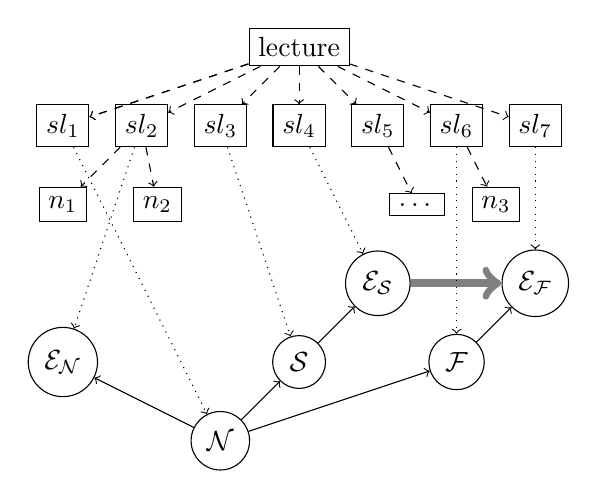
\begin{tikzpicture}
  \begin{scope}[shape=circle]
    \tikzstyle{every node}=[draw]
    \node (N)  at (2,0.5) {$\cal N$};
    \node (EN) at (0,1.5) {$\cal E_N$};
    \node (F)  at (5,1.5) {$\cal F$};
    \node (S)  at (3,1.5) {$\cal S$};
    \node (EF) at (6,2.5) {$\cal E_F$};
    \node (ES) at (4,2.5) {$\cal E_S$};
  \end{scope}
  \draw[->] (N) -- (EN);
  \draw[->] (N) -- (F);
  \draw[->] (N) -- (S);
  \draw[->] (S) -- (ES);
  \draw[->] (F) -- (EF);
  \draw[->,gray,line width=3pt] (ES) -- (EF);
  \begin{scope}
    \tikzstyle{every node}=[draw]
  \node (top) at (3,5.5) {lecture};
  \node (sl1) at (0,4.5) {$sl_1$};
  \node (sl2) at (1,4.5) {$sl_2$};
  \node (sl3) at (2,4.5) {$sl_3$};
  \node (sl4) at (3,4.5) {$sl_4$};
  \node (an) at (4,4.5) {$sl_5$};
  \node (sl5) at (5,4.5) {$sl_6$};
  \node (sl6) at (6,4.5) {$sl_7$};
  \node (n1) at (0,3.5) {$n_1$};
  \node (n2) at (1.2,3.5) {$n_2$};
  \node (n5) at (4.5,3.5){\ldots};
  \node (n6) at (5.5,3.5) {$n_3$};
\end{scope}
  \draw[->,dashed] (top) -- (sl1);
  \draw[->,dashed] (top) -- (sl1);
  \draw[->,dashed] (top) -- (sl2);
  \draw[->,dashed] (top) -- (sl3);
  \draw[->,dashed] (top) -- (sl4);
  \draw[->,dashed] (top) -- (an);
  \draw[->,dashed] (top) -- (sl5);
  \draw[->,dashed] (top) -- (sl6);
  \draw[->,dashed] (sl2) -- (n1);
  \draw[->,dashed] (sl2) -- (n2);
  \draw[->,dashed] (an) -- (n5);
  \draw[->,dashed] (sl5) -- (n6);

  \draw[->,dotted] (sl1) -- (N);
  \draw[->,dotted] (sl2) -- (EN);
  \draw[->,dotted] (sl3) -- (S);
  \draw[->,dotted] (sl4) -- (ES);
  \draw[->,dotted] (sl5) -- (F);
  \draw[->,dotted] (sl6) -- (EF);
\end{tikzpicture}

%%% Local Variables: 
%%% mode: latex
%%% TeX-master: "omdoc"
%%% End: 

% LocalWords:  EF sl

\end{myfig}

The top part of the diagram with the dashed lines stands for the narrative structure,
where the arrows mark up the document structure. For instance, the slides {sl$_i$} are
grouped into a lecture. The dashed lines between the two documents visualize {\omdoc}
references with pointers into the content structure. In the example in
{\myfigref{straw-man}}, the second slide of ``lecture'' presents the first example: the
text fragment {n$_1$} links the content $\cal E_N$, which is referenced from the content
structure, to slide 1. The fragment {n$_2$} might say something like ``this did not work
in the current situation, so we have to extend the conceptualization\ldots''.

Just as for content-based systems on the formula level, there are now MKM systems that
generate presentation markup from content markup, based on general presentation
principles, also on this level. For instance, the {\sc{ActiveMath}}
system~\cite{MelBue:krma03} generates a simple narrative structure (the
presentation; called a personalized book) from the underlying content structure (given in
{\omdoc}) and a user model.
\end{tsection}

\begin{tsection}[id=courseware-summary]{Summary}
As we have seen, the narrative and content fulfill different, but legitimate
content markup needs, that can coincide (as in the main example in this chapter),
but need not (as in the example in the last section). In the simple case, where
the dependency and narrative structure largely coincide, systems like the
{\activemath} system described in {\mysecref{activemath}} can generate narrative
{\omdoc}s from content {\omdoc}s automatically. To generate more complex
{\twintoo{rhetoric/didactic}{figure}s}\twin{didactic}{figure}, we would have to
have more explicit markup for relations like ``can act as a straw-man for''.
Providing standardized markup for such relations is beyond the scope of the
{\omdoc} format, but could easily be expressed as metadata, or as external, e.g.
{\rdf}-based relations.
\end{tsection}
\end{tchapter}


%%% Local Variables: 
%%% mode: latex
%%% TeX-master: "omdoc"
%%% End: 

% LocalWords:  ann kr lst stlc cd ext href jpg ps oo cvi danny pf uri url
% LocalWords:  superclasses Sleator isa dannys def var xref concl EN dc ns elt
% LocalWords:  pto cvic omlet ref otheromgrouptype obj inh inst activemath gif
% LocalWords:  cpoint omcds mowgli EF ES linecolor linewidth sl RDF clas xunit
% LocalWords:  mathescape Courseware courseware mbase CMP FMP OMA OMOBJ thm
% LocalWords:  metadata CDATA omgroup omtext omdoc ActiveMath  ActiveMath
% LocalWords:  ActiveMath MelBue krma03

%%%%%%%%%%%%%%%%%%%%%%%%%%%%%%%%%%%%%%%%%%%%%%%%%%%%%%%%%%%%%%%%%%%%%%%%%
% This file is part of the LaTeX sources of the OMDoc 1.3 specification
% Copyright (c) 2006 Michael Kohlhase
% This work is licensed by the Creative Commons Share-Alike license
% see http://creativecommons.org/licenses/by-sa/2.5/ for details
\svnInfo $Id: xmlrpc.tex 9251 2012-07-23 10:29:02Z kohlhase $
\svnKeyword $HeadURL: https://svn.omdoc.org/repos/omdoc/branches/omdoc-1.3/doc/spec/xmlrpc.tex $
%%%%%%%%%%%%%%%%%%%%%%%%%%%%%%%%%%%%%%%%%%%%%%%%%%%%%%%%%%%%%%%%%%%%%%%%%

\begin{tchapter}[id=rpc,short=Communication between Systems]{Communication with and between Mathematical Software Systems}

{\omdoc} can be used as content language for communication protocols between
mathematical software systems on the Internet. The ability to specify the context
and meaning of the mathematical objects makes the {\omdoc} format ideally suited
for this task.

In this chapter we will discuss a message interface in a fictitious software system
{\mathwebws}\footnote{``{\mathweb} {\bf{W}}eb {\bf{S}}ervices''; The examples discussed in
  this chapter are inspired by the {\mathwebsb}~\cite{FraKoh:mabdl99,ZimKoh:tmsbdmr02}
  (``{\mathweb} {\bf{S}}oftware {\bf{B}}us'') service infrastructure, which offers similar
  functionality based on the {\xmlrpc} protocol (an {\xml} encoding of Remote Procedure
  Calls (RPC)~\cite{xmlrpc}). We use the {\soap}-based formulation, since {\soap}
  ({\bf{S}}imple {\bf{O}}bject {\bf{A}}ccess {\bf{P}}rotocol) is the relevant
  {\indextoo{W3C}} standard and we can show the embedding of {\omdoc} fragments into other
  {\xml} namespaces. In {\xmlrpc}, the {\xml} representations of the content language
  {\omdoc} would be transported as base-64-encoded strings, not as embedded {\xml}
  fragments. }, which connects a wide-range of {\twintoo{reasoning}{system}s}
({\twinemph{mathematical}{service}s}), such as {\atwintoo{automated}{theorem} {prover}s},
{\atwintoo{automated}{proof}{assistant}s}, {\twintoo{computer algebra}{system}s},
{\twintoo{model}{generator}s}, {\twintoo{constraint}{solver}s}, human interaction units,
and {\atwintoo{automated}{concept formation} {system}s}, by a common
{\twinemph{mathematical}{software bus}}.  Reasoning systems integrated in {\mathwebws} can
therefore offer new services to the pool of services, and can in turn use all services
offered by other systems.

On the protocol level, {\mathwebws} uses {\soap} remote procedure calls with the HTTP
binding~\cite{GudHad:soapad03} (see~\cite{Mitra:soapPrimer03} for an introduction to
{\soap}) interface that allows client applications to request service objects and to use
their service methods. For instance, a client can simply request a service object for the
automated theorem prover {\spass}~\cite{Weidenbach:sv97} via the {\http} {\sf{GET}}
request in {\mylstref{discover-spass}} to a {\mathwebws} broker node.

\begin{lstlisting}[label=lst:discover-spass,
          caption={Discovering Automated Theorem Provers (Request)}]
GET /ws.mathweb.org/broker/getService?name=SPASS  HTTP/1.1
Host: ws.mathweb.org
Accept: application/soap+xml
\end{lstlisting}

As a result, the client receives a {\soap} message like the one in
{\mylstref{rpc-spass}} containing information about various instances of
services embodying the {\spass} prover known to the broker service.

\begin{lstlisting}[label=lst:rpc-spass,
          caption={Discovering Automated Theorem Provers (Response)}]
HTTP/1.1 200 OK
Content-Type: application/soap+xml
Content-Length: 990

<?xml version='1.0'?>
<env:Envelope xmlns:env="http://www.w3.org/2003/05/soap-envelope">
  <env:Body>
    <ws:prover env:encodingStyle="http://www.w3.org/2003/05/soap-encoding"
        xmlns:ws="http://www.mathweb.org/ws-fictional">
      <ws:name>SPASS</ws:name>
      <ws:version>2.1</ws:version>
      <ws:URL>http://spass.mpi-sb.mpg.de/webspass/soap</ws:URL>
      <ws:uptime>P3D5H6M45S</ws:uptime>
      <ws:sysinfo>
        <ws:ostype>SunOS 5.6</ws:ostype>
        <ws:mips>3825</ws:mips>
      </ws:sysinfo>
    </ws:prover>
    <ws:prover env:encodingStyle="http://www.w3.org/2003/05/soap-encoding"
        xmlns:ws="http://www.mathweb.org/ws-fictional">
      <ws:name>SPASS</ws:name>
      <ws:version>2.0</ws:version>
      <ws:URL>http://asuka.mt.cs.cmu.edu/atp/spass/soap</ws:URL>
      <ws:uptime>P5M2D15H56M5S</ws:uptime>
      <ws:sysinfo>
        <ws:ostype>linux-2.4.20</ws:ostype>
        <ws:mips>1468</ws:mips>
      </ws:sysinfo>
    <ws:prover>
  </env:Body>
</end:Envelope>
\end{lstlisting}

The client can then select one of the provers (say the first one, because it runs
on the faster machine) and post theorem proving requests like the one in
{\mylstref{rpc-prover}}\footnote{We have made the namespaces involved explicit
  with prefixes in the examples, to show the mixing of different {\xml}
  languages.} to the URL which uniquely identifies the service object in the
Internet (this was part of the information given by the broker; see line 11 in
{\mylstref{rpc-spass}}).

\begin{lstlisting}[label=lst:rpc-prover,
  caption={A {\soap} RPC call to {\spass}}]
POST http://spass.mpi-sb.mpg.de/webspass/soap HTTP/1.1
Host: http://spass.mpi-sb.mpg.de/webspass/soap
Content-Type: application/soap+xml; 
Content-Length: 1123

<?xml version='1.0'?>
<env:Envelope xmlns:env="http://www.w3.org/2003/05/soap-envelope">
  <env:Body>
    <ws:prove env:encodingStyle="http://www.w3.org/2003/05/soap-encoding"
        xmlns:ws="http://www.mathweb.org/ws-fictional">
      <omdoc:assertion xml:id="peter-hates-somebody" type="conjecture"
             xmlns:omdoc="http://omdoc.org/ns"
             theory="http://mbase.mathweb.org:8080/RPC2#lovelife"> 
        <omdoc:CMP>Peter hates somebody</omdoc:CMP> 
        <omdoc:FMP> 
          <om:OMOBJ xmlns:om="http://www.openmath.org/OpenMath"> 
            <om:OMBIND> 
             <om:OMS cd="quant1" name="exists"/> 
             <om:OMBVAR><om:OMV name="X"/></om:OMBVAR> 
             <om:OMA> 
               <om:OMS cd="lovelife" name="hate"/> 
                <om:OMS cd="lovelife" name="peter"/> 
                <om:OMV name="X"/> 
              </om:OMA> 
            </om:OMBIND> 
          </om:OMOBJ> 
        </omdoc:FMP> 
      </omdoc:assertion> 
      <ws:replyWith><ws:state>proof</ws:state></ws:replyWith>
      <ws:timeout>20</ws:timeout>
    </ws:prove>
  </env:Body>
</env:Envelope>
\end{lstlisting}
This {\soap} remote procedure call uses a generic method ``{\snippet{prove}}'' that can be
understood by the {\atwintoo{first-order}{theorem}{prover}s} on {\mathwebsb}, and in
particular the {\spass} system. This method is encoded as a {\element[ns-elt=ws]{prove}}
element; its children describe the proof problem and are interpreted by the {\soap} RPC
node as a parameter list for the method invocation.  The first parameter is an {\omdoc}
representation of the assertion to be proven. The other parameters instruct the theorem
prover service to reply with the proof (instead of e.g. just a yes/no answer) and gives it
a time limit of 20 seconds to find it.

Note that {\omdoc} fragments can be seamlessly integrated into an {\xml} message format
like {\soap}. A {\soap} implementation in the client's implementation language simplifies
this process drastically since it abstracts from {\http} protocol details and offers
{\soap} nodes using data structures of the host language.  As a consequence, developing
{\mathweb} clients is quite simple in such languages.  Last but not least, both {\msie}
and the open source WWW browser {\firefox} now allow to perform {\soap} calls within
JavaScript. This opens new opportunities for building user interfaces based on web
browsers.

Note furthermore that the example in {\mylstref{rpc-prover}} depends on the information
given in the theory {\snippet{lovelife}} referenced in the {\attribute{theory}{assertion}}
attribute in the {\element{assertion}} element (see {\mysecref{theories}} for a
discussion of the theory structure in {\omdoc}). In our instance, this theory might
contain formalizations (in first-order logic) of the information that Peter hates
everybody that Mary loves and that Mary loves Peter, which would allow {\spass} to prove
the assertion. To get the information, the {\mathwebws} service based on {\spass} would
first have to retrieve the relevant information from a knowledge base like the {\mbase}
system described in {\mysecref{mbase}} and pass it to the {\spass} theorem prover as
background information. As {\mbase} is also a {\mathwebws} server, this can be done by
sending the query in {\mylstref{rpc-getTheory}} to the {\mbase} service at
\url{http://mbase.mathweb.org:8080}.

\begin{lstlisting}[label=lst:rpc-getTheory,  
  caption={Requesting a Theory from {\mbase}}]
GET /mbase.mathweb.org:8080/soap/getTheory?name=lovelife  HTTP/1.1
Host: mbase.mathweb.org:8080
Accept: application/soap+xml
\end{lstlisting}
The answer would be of the form given in {\mylstref{rpc-theory}}. Here, the
{\soap} envelope contains the {\omdoc} representation of the requested theory
(irrespective of what the internal representation of {\mbase} was).
\begin{lstlisting}[label=lst:rpc-theory,mathescape,
  caption={The Background Theory for Message {\ref{lst:rpc-prover}}}]
HTTP/1.1 200 OK
Content-Type: application/soap+xml
Content-Length: 602

<?xml version='1.0'?>
<env:Envelope xmlns:env="http://www.w3.org/2003/05/soap-envelope">
  <env:Body>
    <theory xml:id="lovelife" xmlns="http://omdoc.org/ns"> 
      <symbol name="peter"/><symbol name="mary"/> 
      <symbol name="love"/><symbol name="hate"/> 
      <axiom xml:id="opposite"> 
        <CMP><xhtml:p>Peter hates everybody Mary loves</xhtml:p></CMP> 
        <FMP>$\allcdot{x}{loves(mary,x)\Rightarrow hates(peter,x)}$</FMP> 
      </axiom> 
      <axiom xml:id="mary-loves-peter"> 
        <CMP><xhtml:p>Mary loves Peter</xhtml:p></CMP> 
        <FMP>$loves(mary,peter)$</FMP>
      </axiom>
    </theory>
  </env:Body>
</env:Envelope>
\end{lstlisting}
This information is sufficient to prove the theorem in {\mylstref{rpc-prover}}; and the
{\spass} service might reply to the request with the message in {\mylstref{rpc-proof}}
which contains an {\omdoc} representation of a proof (see {\mychapref{proofs}} for
details). Note that the {\attribute{for}{proof}} attribute in the {\element{proof}}
element points to the original assertion from {\mylstref{rpc-prover}}.
\begin{lstlisting}[label=lst:rpc-proof,mathescape,
  caption={A proof that Peter hates someone}]
HTTP/1.1 200 OK
Content-Type: application/soap+xml
Content-Length: 588

<?xml version='1.0'?>
<env:Envelope xmlns:env="http://www.w3.org/2003/05/soap-envelope">
  <env:Body>
    <proof xml:id="p347" for="#peter-hates-somebody"
           xmlns="http://omdoc.org/ns"> 
      <derive xml:id="d1">
        <FMP>$hates(peter,peter)$</FMP>
        <method xref="nd.omdoc#ND.chain">
          <premise xref="#lovelife.mary-loves-peter"/>
          <premise xref="#lovelife.opposite"/>
        </method>
      </derive>
      <derive xml:id="concl">
        <method xref="nd.omdoc#ND.ExI"><premise xref="#d1"/></method>
      </derive>
    </proof>
  </env:Body>
</env:Envelope>
\end{lstlisting} 
The proof has two steps: The first one is represented in the {\element{derive}} element,
which states that ``Peter hates Peter''. This fact is derived from the two axioms in the
theory {\snippet{lovelife}} in {\mylstref{rpc-theory}} (the {\element{premise}} elements
point to them) by the ``chaining rule'' of the
{\atwintoo{natural}{deduction}{calculus}}. This inference rule is represented by a symbol
in the theory {\snippet{ND}} and referred to by the {\attribute{xref}{method}} attribute
in the {\element{method}} element.  The second proof step is given in the second
{\element{derive}} element and concludes the proof. Since the assertion of the conclusion
is the statement of the proven assertion, we do not have a separate {\element{FMP}}
element that states this here. The sole premise of this proof step is the previous one.
For details on the representation of proofs in {\omdoc} see {\mychapref{proofs}}.

Note that the {\spass} theorem prover does not in itself give proofs in the
{\atwintoo{natural}{deduction}{calculus}}, so the {\spass} service that provided this
answer presumably enlisted the help of another {\mathwebws} service like the {\tramp}
system~\cite{Meier:sdttom00} that transforms resolution proofs (the native format of the
{\spass} prover) to natural deduction proofs.
\end{tchapter}

%%% Local Variables: 
%%% mode: latex
%%% TeX-master: "omdoc"
%%% End: 

% LocalWords:  xmlrpc spass methodCall methodName getService params param CMP
% LocalWords:  struct lovelife FMP cd quant replyWith timeout JavaScript mary
% LocalWords:  getTheory mathescape methodResponse lst int xref concl ExI msie
% LocalWords:  nnnn env encodingStyle uptime sysinfo ostype SunOS mips omdoc om
% LocalWords:  mbase rpc eb ervices oftware imple bject ccess rotocol xmlns ws
% LocalWords:  ns elt OMOBJ OMBIND OMBVAR OMV OMA kohlhase tchapter mathwebws
% LocalWords:  mathweb mathwebsb FraKoh mabdl99 ZimKoh tmsbdmr02 indextoo
% LocalWords:  twintoo twinemph atwintoo GudHad soapad03 mylstref lstlisting
% LocalWords:  mysecref allcdot Rightarrow mychapref nd.omdoc sdttom00


%%%%%%%%%%%%%%%%%%%%%%%%%%%%%%%%%%%%%%%%%%%%%%%%%%%%%%%%%%%%%%%%%%%%%%%%%
% This file is part of the LaTeX sources of the OMDoc 1.3 specification
% Copyright (c) 2006 Michael Kohlhase
% This work is licensed by the Creative Commons Share-Alike license
% see http://creativecommons.org/licenses/by-sa/2.5/ for details
%%%%%%%%%%%%%%%%%%%%%%%%%%%%%%%%%%%%%%%%%%%%%%%%%%%%%%%%%%%%%%%%%%%%%%%%%

\part{The OMDoc Document Format}\label{part:specification}
  The {\omdoc} (\underline{O}pen \underline{M}athematical \underline{Doc}uments) format is
  a content markup scheme for (collections of) mathematical documents including articles,
  textbooks, interactive books, and courses.  {\omdoc} also serves as the content language
  for agent communication of mathematical services on a mathematical software bus.

  This part of the {\report} is the specification of version 1.3 of the {\omdoc} format,
  the final and mature release of {\omdoc} version 1. It defines the {\omdoc} language
  features and their meaning. The content of this part is normative for the {\omdoc}
  format; an {\omdoc} document is valid as an {\omdoc} document, iff it meets all the
  constraints imposed here. {\omdoc} applications will normally presuppose valid {\omdoc}
  documents and only exhibit the intended behavior on such.




%%% Local Variables: 
%%% mode: latex
%%% TeX-master: "omdoc"
%%% End: 

% LocalWords:  mypart tocdepth athematical uments
%%% the specification part
%%%%%%%%%%%%%%%%%%%%%%%%%%%%%%%%%%%%%%%%%%%%%%%%%%%%%%%%%%%%%%%%%%%%%%%%%
% This file is part of the LaTeX sources of the OMDoc 1.3 specification
% Copyright (c) 2006 Michael Kohlhase
% This work is licensed by the Creative Commons Share-Alike license
% see http://creativecommons.org/licenses/by-sa/2.5/ for details
%%%%%%%%%%%%%%%%%%%%%%%%%%%%%%%%%%%%%%%%%%%%%%%%%%%%%%%%%%%%%%%%%%%%%%%%%
\begin{tchapter}[id=spec-intro]{General Aspects of the OMDoc Format}
\ednote{MK: some intro here.}
\begin{tsection}[id=modular]{OMDoc as a Modular Format}
  A modular approach to design is generally accepted as best practice in the development
  of any type of complex application. It separates the application's functionality into a
  number of "{\indextoo{building blocks}}" or "{\indextoo{module}s}", which are
  subsequently combined according to specific rules to form the entire application. This
  approach offers numerous advantages: The increased {\indextoo{conceptual clarity}}
  allows developers to share ideas and code, and it encourages reuse by creating
  well-defined modules that perform a particular task. Modularization also reduces
  complexity by decomposition of the application's functionality and thus decreases
  debugging time by localizing errors due to design changes. Finally, flexibility and
  maintainability of the application are increased because single modules can be upgraded
  or replaced independently of others.

  The {\omdoc} vocabulary has been split by thematic role, which we will briefly overview
  in {\myfigsref{core-modules}{ext-modules}} before we go into the specifics of the respective modules
  in {\mychaplref{mobj}{quiz}}. To avoid repetition, we will introduce some attributes
  already in this chapter that are shared by elements from all modules. In
  {\mychapref{document-model}} we will discuss the {\omdoc} document model and possible
  sub-languages of {\omdoc} that only make use of parts of the functionality
  (\mysecref{sub-languages}).

\begin{myfig}{core-modules}{The {\omdoc} Modules}
\begin{small}
\fbox{\begin{tabular}{|l|l|l|l|}\hline
  Module & Title & Required? & Chapter\\\hline\hline
  {\bf\MOBJmodule{spec}} &  Mathematical Objects & yes & {\mychapref{mobj}}\\\hline
    \multicolumn{4}{|p{11cm}|}{\em\footnotesize Formulae are a central part of mathematical
       documents; this module integrates the content-oriented representation
       formats {\openmath} and {\mathml} into {\omdoc}}\\\hline\hline
  {\bf\MTXTmodule{spec}} &  Mathematical Text & yes & {\mychapref{mtxt}}\\\hline
    \multicolumn{4}{|p{11cm}|}{\em\footnotesize Mathematical vernacular,
  i.e. natural language with embedded formulae}\\\hline\hline
  {\bf\DOCmodule{spec}} & Document Infrastructure & yes & {\mychapref{omdoc-infrastructure}}\\\hline
    \multicolumn{4}{|p{11cm}|}{\em\footnotesize  A basic infrastructure for
      assembling pieces of  mathematical knowledge into functional documents and 
      referencing their parts }\\\hline\hline
  {\bf\RTmodule{spec}} & Rich Text Structure & no & {\mysecref{rt}}\\\hline
    \multicolumn{4}{|p{11cm}|}{\em\footnotesize Rich text structure in
  mathematical vernacular (lists, paragraphs, tables, \ldots)}\\\hline\hline
  {\bf\STmodule{spec}} &  Mathematical Statements & no  & {\mychapref{statements}}\\\hline
    \multicolumn{4}{|p{11cm}|}{\em\footnotesize Markup for mathematical forms like 
      {\indextoo{theorem}s},  {\indextoo{axiom}s}, {\indextoo{definition}s}, 
      and {\indextoo{example}s} that can be used to specify or define properties
      of given mathematical objects and theories to group mathematical
  statements and provide a notion of context.}\\\hline\hline
  {\bf\PFmodule{spec}} &  Proofs and proof objects & no & {\mychapref{proofs}}\\\hline 
    \multicolumn{4}{|p{11cm}|}{\em\footnotesize Structure of proofs
     and argumentations at various levels of details and formality}\\\hline\hline
 {\bf\PRESmodule{spec}} & Presentation Information & no &  {\mychapref{pres}}\\\hline
    \multicolumn{4}{|p{11cm}|}{\em\footnotesize Limited functionality for
    specifying presentation and notation information for local typographic
      conventions  that cannot be determined by general principles alone}\\\hline\hline
 \end{tabular}}
\end{small}
\end{myfig}
The modules in {\myfigref{core-modules}} are required (mathematical documents without them
do not really make sense), the ones in {\myfigref{ext-modules}} are optional.

The document-structuring elements in module {\DOCmodule{spec}} have an attribute
{\attributeshort{modules}} that allows to specify which of the modules are used in a
particular document (see {\mychapref{omdoc-infrastructure}} and
{\mysecref{sub-languages}}).
\begin{myfig}{ext-modules}{The {\omdoc} Modules}
\begin{small}
\fbox{\begin{tabular}{|l|l|l|l|}\hline
  Module & Title & Required? & Chapter\\\hline\hline
 {\bf\DCmodule{spec}} & Dublin Core Metadata & yes &   {\mysecsref{dc-elements}{dc-roles}}\\\hline
    \multicolumn{4}{|p{11cm}|}{\em\footnotesize Contains bibliographical ``{\twindef{data}{about data}}'',
      which can be used to annotate many {\omdoc} elements by descriptive and
      administrative information that facilitates navigation and organization}\\\hline\hline 
  {\bf\CCmodule{spec}} & Creative Commons Metadata & yes & {\mysecref{creativecommons}}\\\hline
    \multicolumn{4}{|p{11cm}|}{\em\footnotesize Licenses for text use}\\\hline\hline
 {\bf\ADTmodule{spec}} &  Abstract Data Types & no & {\mychapref{adt}}\\\hline 
    \multicolumn{4}{|p{11cm}|}{\em\footnotesize  Definition schemata for
      sets that are built up inductively from constructor symbols}\\\hline\hline 
  {\bf\CTHmodule{spec}} & Complex Theories & no & {\mychapref{complex-theories}}\\\hline
    \multicolumn{4}{|p{11cm}|}{\em\footnotesize Theory morphisms; they can be used
    to structure mathematical theories}\\\hline\hline
  {\bf\DGmodule{spec}} & Development Graphs & no & {\mysecref{development-graphs}}\\\hline
    \multicolumn{4}{|p{11cm}|}{\em\footnotesize Infrastructure for managing theory
  inclusions, change management}\\\hline\hline
  {\bf\EXTmodule{spec}} & Applets, Code, and Data & no & {\mychapref{ext}}\\\hline
    \multicolumn{4}{|p{11cm}|}{\em\footnotesize Markup for applets, program code,
  and data (e.g. images, measurements, \ldots)}\\\hline\hline
 {\bf\QUIZmodule{spec}} &  Infrastructure for Assessments & no & {\mychapref{quiz}}\\\hline
    \multicolumn{4}{|p{11cm}|}{\em\footnotesize Markup for exercises integrated
    into the {\omdoc} document model}\\\hline 
  \end{tabular}}
\end{small}
\end{myfig}
\end{tsection}

\begin{tsection}[id=omdoc-ns]{The OMDoc Namespaces}
  
  The namespace for the {\omdoc} format is the URI\atwin{OMDoc}{namespace}{URI}
  \url{http://omdoc.org/ns}. Note that the {\omdoc}
  namespace\twin{OMDoc}{namespace} does not reflect the versions, this is done in the
  {\attributeshort{version}} attribute on the {\twintoo{document}{root}} element
  {\element{omdoc}} (see {\mychapref{omdoc-infrastructure}}).  As a consequence, the
  {\omdoc} vocabulary identified by this namespace is not static, it can change with each
  new {\omdoc} version. However, if it does, the changes will be documented in later
  versions of the specification: the latest released version can be found
  at~\cite{URL:omdocspec}.


  \begin{myfig}{omdoc-namespaces}{OMDoc Namespaces}\scriptsize
    \begin{tabular}{|l|l|l|}\hline
      Format      & namespace URI & see \\\hline\hline
      Dublin Core & \url{http://purl.org/dc/elements/1.1/} &   {\mysecsref{dc-elements}{dc-roles}}\\\hline
      Creative Commons & \url{http://creativecommons.org/ns} & {\mysecref{creativecommons}}\\\hline
      {\mathml} & \url{http://www.w3.org/1998/Math/MathML} & {\mysecref{cmml}}\\\hline
      {\openmath} & \url{http://www.openmath.org/OpenMath} & {\mysecref{openmath}}\\\hline
      {\xslt} & \url{http://www.w3.org/1999/XSL/Transform} & {\mychapref{pres}}\\\hline
    \end{tabular}
  \end{myfig}
  In an {\omdoc} document, the {\omdoc} namespace must be specified either using a
  {\twintoo{namespace}{declaration}} of the form
  {\snippet{xmlns="}}\url{http://omdoc.org/ns}{\snippet{"}} on the {\element{omdoc}}
  element or by prefixing the {\twintoo{local}{name}s} of the {\omdoc} elements by a
  namespace prefix ({\omdoc} customarily use the prefixes {\snippet{omdoc:}} or
  {\snippet{o:}}) that is declared by a {\atwintoo{namespace}{prefix}{declaration}} of the
  form {\snippet{xmlns:o="}}\url{http://omdoc.org/ns}{\snippet{"}} on some element
  dominating the {\omdoc} element in question (see {\mysecref{xml}} for an
  introduction). {\omdoc} also uses the namespaces in
  \myfigref{omdoc-namespaces}\footnote{In this specification we will use the
    {\twintoo{namespace}{prefix}es} above on all the elements we reference in text unless
    they are in the {\omdoc} namespace.}  Thus a typical document root of an {\omdoc}
  document looks as follows:
  \begin{lstlisting}[mathescape]
<?xml version="1.0" encoding="utf-8"?>
<omdoc xml:id="test.omdoc" version="1.3"
  xmlns="http://omdoc.org/ns"
  xmlns:cc="http://creativecommons.org/ns"
  xmlns:dc="http://purl.org/dc/elements/1.1/"
  xmlns:om="http://www.openmath.org/OpenMath"
  xmlns:m="http://www.w3.org/1998/Math/MathML">
$\ldots$
</omdoc>
\end{lstlisting}  
\end{tsection}

\begin{tsection}[id=common-attribs]{Common Attributes in OMDoc}
  There are some attributes that are common to many {\omdoc} elements, so we will describe
  them here before we go into the specifics of the respective elements themselves

  \begin{tsubsection}[id=foreign-attribs]{Foreign-Namespace Attributes}

  Generally, the {\omdoc} format allows any attributes from foreign (i.e. non-{\omdoc})
  namespaces\twin{foreign}{namespace} on the {\omdoc} elements. This is a commonly found
  feature that makes the {\xml} encoding of the {\omdoc} format extensible. Note that the
  attributes defined in this specification are in the default (empty)
  namespace\twin{default}{namespace}\twin{empty}{namespace}: they do not carry a namespace
  prefix. So any attribute of the form {\snippet{na:xxx}} is allowed as long as it is in
  the scope of a suitable {\atwintoo{namespace}{prefix}{declaration}}.
\end{tsubsection}

\begin{tsubsection}[id=identifiers]{XML Identifiers}
  Many {\omdoc} elements have optional {\attributeshort[ns-attr=xml]{id}} attributes that
  can be used as identifiers to reference them. These attributes are of type
  {\snippet{ID}}\twin{type}{ID}, they must be unique in the document which is important,
  since many {\xml} applications\twin{XML}{application} offer functionality for
  referencing and retrieving elements by {\snippet{ID}}-type\twin{type}{ID} attributes.
  Note that unlike other {\snippet{ID}}{\twin{ID}{type}}-attributes, in this special case
  it is the name {\attributeshort[ns-attr=xml]{id}}~\cite{XML:id05} that defines the
  {\indextoo{referencing}} and {\indextoo{uniqueness}} functionality, not the type
  declaration in the {\indextoo{DTD}} or {\twintoo{XML}{schema}} (see
  {\mysubsecref{xml-validation}} for a discussion).

  Note that in the {\omdoc} format proper, all {\twintoo{ID}{type}} attributes are of the
  form {\attributeshort[ns-attr=xml]{id}}. However in the older {\openmath} and {\mathml}
  standards, they still have the form {\attributeshort{id}}. The latter are only
  recognized to be of type {\snippet{ID}}, if a document type or {\xml}schema is
  present. Therefore it depends on the application context, whether a DTD should be
  supplied with the {\omdoc} document.
\end{tsubsection}

\begin{oldpart}{MK:this needs some rework, in particular, we have to cite CSS 2.1 and say
    that the cascading rules of that apply.}
\begin{tsubsection}[id=css-attribs]{CSS Attributes}
  For many occasions (e.g. for printing {\omdoc} documents), authors want to control a
  wide variety of aspects of the presentation. {\omdoc} is a content-oriented format, and
  as such only supplies an infrastructure to mark up content-relevant information in
  {\omdoc} elements. To address this dilemma {\xml} offers an interface to 
  {\twintoo{Cascading}{Style Sheet}s} ({\css})~\cite{BosHak:css98}, which allow to specify
  presentational traits like {\twintoo{text}{color}}, {\twintoo{font}{variant}},
  {\indextoo{positioning}}, {\indextoo{padding}}, or {\indextoo{frame}s} of
  {\twintoo{layout}{box}es}, and even {\indextoo{aural}} aspects of the text.
  
  To make use of {\css}, most {\omdoc} elements (all that have
  {\attributeshort[ns-attr=xml]{id}} attributes) have {\attributeshort{style}}
  attributes\footnote{The treatment of the {\css} attributes has changed from
    {\omdocv{1.1}}, see the discussion on
    page~\pageref{style/class-comment}.}\twin{CSS}{attribute} that can be used to specify
  {\css} directives\twin{CSS}{directive} for them. In the {\omdoc} fragment in
  {\mylstref{css-basic}} we have used the {\attribute{style}{omtext}} attribute to specify
  that the text content of the {\element{omtext}} element should be formatted in a
  centered box whose width is 80\% of the surrounding box (probably the page box), and
  that has a 2 pixel wide solid frame of the specified RGB color. Generally {\css}
  directives are of the form {\snippet{A:V}}, where {\snippet{A}} is the name of the
  aspect, and {\snippet{V}} is the value, several {\css} directives\twin{CSS}{directive}
  can be combined in one {\attributeshort{style}} attribute as a
  {\twintoo{semicolon-separated}{list}} (see {\cite{BosHak:css98} and the emerging {\css}
    3} standard).

\begin{lstlisting}[label=lst:css-basic,mathescape,
   caption={Basic {\css} Directives in a {\attributeshort{style}} Attribute},
   index={style,class}]
<?xml version="1.0" encoding="utf-8"?>
<?xml-stylesheet type="text/css" href="http://example.org/style.css"?>
<omdoc xml:id="stylish">
  $\ldots$
  <omtext xml:id="t1" style="width:80%;align:center;border:2px #006699 solid">
    <CMP><xhtml:p>Here comes something 
      <xhtml:span style="font-weight:bold;color:green" class="emphasize">stylish</xhtml:span>!
    </xhtml:p></CMP>
  </omtext>
  $\ldots$
</omdoc>
\end{lstlisting}

Note that many {\css} properties of parent elements are inherited by the children,
if they are not explicitly specified in the child. We could for instance have set
the {\twintoo{font}{family}} of all the children of the {\element{omtext}} element
by adding a directive {\snippet{font-family:sans-serif}} there and then override it by
a directive for the property {\snippet{font-family}} in one of the children.

Frequently recurring groups of {\css} directives can be given symbolic names in {\css}
style sheets\twin{CSS}{style sheet}, which can be referenced by the
{\attributeshort{class}} attribute. In {\mylstref{css-basic}} we have made use of this
with the class {\snippet{emphasize}}, which we assume to be defined in the style sheet
{\snippet{style.css}} associated with the document in the ``{\twintoo{style
    sheet}{processing instruction}}'' in the prolog\footnote{i.e. at the very beginning of
  the {\xml} document before the document type declaration} of the {\xml} document
(see~\cite{Clark:assxd99} for details).  Note that an {\omdoc} element can have both
{\attributeshort{class}} and {\attributeshort{style}} attributes, in this case, precedence
is determined by the rules for {\css} style sheets as specified in~\cite{BosHak:css98}. In
our example in {\mylstref{css-basic}} the directives in the {\attributeshort{style}}
attribute take precedence over the {\css} directives in the style sheet referenced by the
{\attributeshort{class}} attribute on the {\element{xhtml:span}} element. As a
consequence, the word ``stylish'' would appear in green, bold italics.
\end{tsubsection}
\end{oldpart}
\end{tsection}

\begin{tsection}[id=sharing,short=Structure Sharing]{Structure Sharing}

  {\omdoc} is a content markup format, from which documents are produced via a
  presentation process. This ``source character'' of {\omdoc} documents allows to utilize
  structure sharing technologies in the markup\footnote{{\omdocv{1.2}} used the
    {\oldelement{ref}{1.2}} element with {\oldattribute{type}{ref}{1.2}}
    {\oldattval{include}{type}{ref}{1.2}} for this purpose. The new
    {\attributeshort{tref}}-based infrastructure supports validation much better.}. For
  structure sharing {\omdoc} uses the {\attributeshort{tref}} attribute: all content
  elements\ednote{MK: what are they? Intuitively, all that allow the id attributes and
    metadata children. If that is true, we can maybe optimize the schema further.} can be
  used with the {\attributeshort{tref}} whose value is a URI reference to an {\omdoc}
  element instead of the normal element models. We call such an element an
  {\twindef{OMDoc}{reference}}\ednote{MK: probably better use \texttt{oref}
    instead}. Semantically, {\omdoc} references are just placeholders for the {\omdoc}
  objects they reference via their {\attributeshort{tref}} attribute. {\omdoc} references
  require {\omdoc} applications to process the document as if the {\omdoc} reference were
  replaced with the {\omdoc} fragment referenced in the {\attributeshort{tref}} attribute.

  \begin{tsubsection}[id=flattning]{Ref-Reduction and Flattening}

\setbox0=\hbox{\begin{minipage}{5.1cm}
\begin{lstlisting}[label=flattena,mathescape,frame=none,numbers=none,index={omgroup,omtext}]
<omgroup xml:id="text" 
         type="sequence">
  <omtext xml:id="t1">$T_1$</omtext>
  <omgroup xml:id="enum" 
            type="enumeration">
    <omtext xml:id="t2">$T_2$</omtext>
    <omtext xml:id="t3">$T_3$</omtext>
  </omgroup>
  <omtext xml:id="t4">$T_4$</omtext>
</omgroup>
\end{lstlisting}
\end{minipage}}
\setbox1=\hbox{\begin{minipage}{5.5cm}
\begin{lstlisting}[label=flattenb,mathescape,frame=none,numbers=none,index={omgroup,omtext}]
<omgroup xml:id="text" type="sequence">
  <omtext tref="#t1"/>
  <omgroup tref="#enum"/>
  <omtext tref="#t4"/>
</omgroup>

<ignore type="targets"
        comment="already referenced"> 
  <omtext xml:id="t1">$T_1$</omtext>
  <omtext xml:id="t2">$T_2$</omtext>
  <omtext xml:id="t3">$T_3$</omtext>
  <omtext xml:id="t4">$T_4$</omtext>

  <omgroup xml:id="enum" 
           type="enumeration">
    <omtext tref="#t2"/>
    <omtext tref="#t3"/>
  </omgroup>
</ignore>
\end{lstlisting}
\end{minipage}}
\begin{myfig}{flatten}{Flattening a Tree Structure}
\fbox{\box0}$\;\leftrightarrow\;$\fbox{\box1}
\end{myfig}

Let $R$ be an {\omdoc} reference, we call the element the URI in the
{\attributeshort{tref}} points to its {\defin{target}}.  We call the process of replacing
an {\omdoc} reference by its target in a document \twindef{reference}{reduction}, and the
document resulting from the process of systematically and recursively reducing all the
{\omdoc} references the {\atwindef{ref}{normal}{form}} of the source document. Note that
ref-normalization may not always be possible, e.g.  if the ref-targets do not exist or are
inaccessible --- or worse yet, if the relation given by the {\omdoc} references is
{\indextoo{cyclic}}. Moreover, even if it is possible to ref-normalize, this may not lead
to a valid {\omdoc} document, e.g.  since {\snippet{ID}} type\twin{ID}{type} attributes
that were unique in the target documents are no longer in the ref-reduced
one. We will call a document {\defin{ref-reducible}}, iff its ref-normal form exists, and
\defin{ref-valid}, iff the ref-normal form exists and is a valid {\omdoc} document.
  
Note that it may make sense to use documents that are not ref-valid for
{\indextoo{narrative-centered}} documents, such as courseware or slides for talks that
only allude to, but do not fully specify the knowledge structure of the mathematical
knowledge involved. For instance the slides discussed in {\mysecref{narrative-structured}}
do not contain the {\element{theory}} elements that would be needed to make the documents
ref-valid.

{\omdoc} references also allow to ``{\indextoo{flatten}}'' the tree structure in a
document into a list of leaves and relation declarations (see {\myfigref{flatten}} for an
example). It also makes it possible to have more than one view on a document using
{\element{omgroup}} structures that reference a shared set of {\omdoc} elements. Note that
we have embedded the ref-targets of the top-level {\element{omgroup}} element
into an {\element{ignore}} comment, so that an {\omdoc} transformation (e.g. to text form)
does not encounter the same content twice.
\end{tsubsection}

\begin{oldpart}{MK: this needs to be reworked, we also need to think about whether we want
    to do similar cascading for metadata.}
\begin{tsubsection}[id=tref-css-cascading]{Cascading of CSS Attributes}
  While the {\omdoc} approach to specifying document structure is a much more flexible
  (database-like) approach to representing structured documents\footnote{The simple tree
    model is sufficient for simple markup of existing mathematical texts and to replay
    them verbatim in a browser, but is insufficient e.g. for generating individualized
    presentations at multiple levels of abstractions from the representation. The {\omdoc}
    text model --- if taken to its extreme --- allows to specify the respective role and
    contributions of smaller text units, even down to the sub-sentence level, and to make
    the structure of mathematical texts machine-understandable. Thus, an advanced
    presentation engine like the {\activemath} system~\cite{SieBen:acgap00} can --- for
    instance --- extract document fragments based on the preferences of the respective
    user.}  than the tree model, it puts a much heavier load on a system for presenting
  the text to humans. In essence the presentation system must be able to recover the left
  representation from the right one in {\myfigref{flatten}}.  Generally, any {\omdoc}
  element defines a fragment of the {\omdoc} it is contained in: everything between the
  start and end tags and (recursively) those elements that are reached from it by
  following the {\omdoc} references.  In particular, the text fragment corresponding to
  the element with {\attribute[ns-attr=xml]{id}{omtext}}={\snippet{"text"}} in the right
  {\omdoc} of~\myfigref{flatten} is just the one on the left.

  In {\mysecref{common-attribs}} we have introduced the {\css}
  attributes\twin{CSS}{attribute} {\attribute{style}{ref}} and {\attribute{class}{ref}},
  which are present on all {\omdoc} elements. In the case of a {\omdoc} reference, there
  is a problem, since the content of these can be incompatible. In general, the rule for
  determining the style information for an element is that we treat the replacement
  element as if it were a child of the reference, and then determine the values of the
  {\css} properties\twin{CSS}{property} of the {\omdoc} reference by inheritance.
\end{tsubsection}
\end{oldpart}
\end{tsection}

\end{tchapter}
%%% Local Variables: 
%%% mode: latex
%%% TeX-master: "omdoc"
%%% End: 


% LocalWords:  omdoc mobj attribs DTD XMLSchema dtd css omtext RGB
% LocalWords:  lst emph xml utf stylesheet href DOCTYPE px CMP serif ns dc attr
% LocalWords:  xmlns creativecommons cmml openmath cc om mtxt rt adt ext pres
% LocalWords:  na xxx es sans mathescape prolog

%%%%%%%%%%%%%%%%%%%%%%%%%%%%%%%%%%%%%%%%%%%%%%%%%%%%%%%%%%%%%%%%%%%%%%%%%
% This file is part of the LaTeX sources of the OMDoc 1.3 specification
% Copyright (c) 2006 Michael Kohlhase
% This work is licensed by the Creative Commons Share-Alike license
% see http://creativecommons.org/licenses/by-sa/2.5/ for details
\svnInfo $Id: document.tex 9251 2012-07-23 10:29:02Z kohlhase $
\svnKeyword $HeadURL: https://svn.omdoc.org/repos/omdoc/branches/omdoc-1.3/doc/spec/document.tex $
%%%%%%%%%%%%%%%%%%%%%%%%%%%%%%%%%%%%%%%%%%%%%%%%%%%%%%%%%%%%%%%%%%%%%%%%%

\begin{tchapter}[id=omdoc-infrastructure,short=Document Infrastructure]{Document Infrastructure (Module {\DOCmodule{spec}})}

Mathematical knowledge is largely communicated by way of a specialized set of
documents (e.g. e-mails, letters, pre-prints, journal articles, and textbooks).
These employ special notational conventions and visual
representations to convey the mathematical knowledge reliably and efficiently.

When marking up mathematical knowledge, one always has the choice whether to mark up the
structure of the document itself, or the structure of the mathematical knowledge that is
conveyed in the document. Even though in most documents, the document structure is
designed to help convey the structure of the knowledge, the two structures need not be the
same.  To frame the discussion we will distinguish two aspects of mathematical
documents. In the {\twinemph{knowledge-centered}{view}} we organize the mathematical
knowledge by its function, and do not care about a way to present it to human
recipients. In the {\twinemph{narrative-centered}{view}} we are interested in the
structure of the argument that is used to convey the mathematical knowledge to a human
user.

We will call a document {\defin{knowledge-structured}} and
{\defemph{narrative-struc\-tu\-red}}\index{narrative-structured}, based on which of the
two aspects is prevalent in the organization of the material.  Narrative-structured
documents in mathematics are generally directed at human consumption (even without being
in presentation markup). They have a general narrative structure: text interleaving with
formal elements like assertions, proofs, \ldots Generally, the order of presentation plays
a role in their effectiveness as a means of communication.  Typical examples of this class
are course materials or introductory textbooks.  Knowledge-structured documents are
generally directed at machine consumption or for referencing. They do not have a linear
narrative spine and can be accessed randomly and even re-ordered without information loss.
Typical examples of these are formula collections, {\openmath} content dictionaries,
technical specifications, etc.

The distinction between knowledge-structured and narrative-structured documents is
reminiscent of the {\indextoo{presentation}} vs.  {\indextoo{content}}
distinction\index{distinction!presentation vs. content} discussed in
{\mysecref{math-objects}}, but now it is on the level of document structure.  Note that
mathematical documents are often in both categories: a mathematical textbook can be read
from front to end, but it can also be used as a reference, accessing it by the index and
the table of contents.  The way humans work with knowledge also involves a change of
state. When we are taught or explore a mathematical domain, we have a linear/narrative
path through the material, from which we abstract more and more, finally settling for a
semantic representation that is relatively independent from the path we acquired it by.
Systems like {\activemath} (see {\mysecref{activemath}}) use the {\omdoc} format in
exactly that way playing on the difference between the two classes and generating
narrative-structured representations from knowledge-structured ones on the fly.

So, maybe the best way to think about this is that the question whether a document
is narrative- or knowledge-structured is not a property of the document itself,
but a property of the application processing this document.

{\omdoc} provides markup infrastructure for both aspects. In this chapter, we will discuss
the infrastructure for the narrative aspect --- for a working example we refer the reader
to {\mychapref{courseware}}. We will look at markup elements for knowledge-structured
documents in {\mysecref{theories}}.

Even though the infrastructure for narrative aspects of mathematical documents is somewhat
presentation-oriented, we will concentrate on content-markup for it. In particular, we
will not concern ourselves with questions like font families, sizes, alignment, or
positioning of text fragments. Like in most other {\xml} applications, this kind of
information can be specified in the {\css} {\attributeshort{style}} and
{\attributeshort{class}} attributes described in {\mysecref{common-attribs}}.

\begin{tsection}[id=root]{The Document Root}
  
  The {\xml} root element of the {\omdoc} format is the {\eldef{omdoc}} element, it
  contains all other elements described here. We call an {\omdoc} element a
  {\twindef{top-level}{element}}, if it can appear as a direct child of the
  {\element{omdoc}} element.
  
  The {\element{omdoc}} element (and the {\element{omgroup}} element introduced below as
  well) has an optional attribute {\attribute[ns-attr=xml]{id}{omdoc}} that can be used to
  reference the whole document. The {\attribute{version}{omdoc}} attribute is used to
  specify the version of the {\omdoc} format the file conforms to.  It is fixed to the
  string {\snippet{1.3}} by this specification.  This will prevent validation with a
  different version of the {\indextoo{DTD}} or {\indextoo{schema}}, or processing with an
  application using a different version of the {\omdoc} specification. The (optional)
  attribute {\attributeshort{modules}} allows to specify the {\omdoc} modules that are
  used in this document. The value of this attribute is a whitespace-separated list of
  module identifiers (e.g. {\MOBJmodule{spec}} the left column in
  {\myfigref{omdoc-modules}}), {\omdoc} sub-language identifiers (see
  {\myfigref{omdoc-sub-languages}}), or {\twintoo{URI}{reference}s} for externally given
  {\omdoc} modules or sub-language identifiers.\footnote{Allowing these external module
    references keeps the {\omdoc} format extensible. Like in the case with
    {\twintoo{namespace}{URI}s} {\omdoc} do not mandate that these
    {\twintoo{URI}{reference}s} reference an actual resource. They merely act as
    identifiers for the modules.} The intention is that if present, the
  {\attributeshort{modules}} specifies the list of all the modules used in the document
  (fragment).  If a {\attributeshort{modules}} attribute is present, then it is an error,
  if the content of this element contains elements from a module that is not specified;
  spurious module declarations in the {\attribute{modules}{omdoc}} attributes are allowed.
  
  The {\element{omdoc}} element acts as an implicit grouping element, just as the
  {\element{omgroup}} element to be introduced in {\mysecref{sectioning}}. Both have an
  optional {\attribute{type}{omdoc}} attribute; we will discuss its values and meaning in
  {\mysecref{sectioning}}.
  
  Here and in the following we will use tables as the one in {\myfigref{qtgeneral}} to
  give an overview over the respective {\omdoc} elements described in a chapter or
  section.  The first column gives the element name, the second and third columns specify
  the required and optional attributes. We will use the fourth column labeled ``DC'' to
  indicate whether an {\omdoc} element can have a {\element{metadata}} child, which will
  be described in the next section.  Finally the fifth column describes the content model
  --- i.e. the allowable children --- of the element. For this, we will use a form of
  Backus Naur Form notation\twin{Backus Naur form}{notation} also used in the DTD:
  {\snippet{\#PCDATA}} stands for ``{\twintoo{parsed}{character data}}'', i.e. text
  intermixed with legal {\omdoc} elements.) A synopsis of all elements is provided in
  {\myappchapref{table}}.

\begin{myfig}{qtgeneral}{{\omdoc} Elements for Specifying  Document Structure.}
\begin{scriptsize}
\begin{tabular}{|>{\tt}l|>{\tt}p{1truecm}|>{\tt}p{4truecm}|c|>{\tt}p{3.1truecm}|}\hline
{\rm Element}& \multicolumn{2}{l|}{Attributes\hspace*{2.25cm}} & D & Content  \\\hline
             & {\rm Required}  & {\rm Optional}      & C &           \\\hline\hline
 omdoc       &  version, xmlns 
                    & xml:id, type, class, style,  
                       version, modules, theory      & +  &
                       \llquote{front},(\llquote{top-level})*,\llquote{back} \\\hline
\llquote{back} & && index?,bibliography?\\\hline
\llquote{front} & && tableofcontents?\\\hline
 omgroup     &   & xml:id, modules, type, class, style, theory
                                                     & +  & (\llquote{top-level})* \\\hline
 metadata    &   & xml:id, class, style        & -- & \llquote{MDelt}*\\\hline
 ref         & xref & xml:id, type, class, style             & -- &     \\\hline
 ignore      &      & xml:id, type, comment                  & -- & ANY\\\hline
 index     &      & xml:id                  & -- & EMPTY\\\hline
 bibliography    & files  & xml:id                  & -- & EMPTY\\\hline
 \multicolumn{5}{|p{11cm}|}{where \llquote{top-level} stands for top-level {\omdoc} elements, and
   \llquote{MDelt} for those introduced in {\mychapref{metadata}}}\\\hline
\end{tabular}
\end{scriptsize}
\end{myfig}
\end{tsection}

\begin{newpart}{MK: we needed to introduce this, but the text is still very rough around
    the edges. Moreover, we should look at traditional front matter, which probably are
    things like abstract, acknowledgements, .... these need to be modeled as well. Also
    think about sectionalfrontmatter and sectional back matter, e.g. get inspired by the
    way LTXML treats them.}
\begin{tsection}[id=frontbackmatter]{Front/Backmatter}
  Documents usually have {\twin{front}{matter}} and {\twin{back}{matter}}, {\omdoc} is no
  exception. Currently, the {\omdoc} front matter only consists of the
  {\element{tableofcontents}} element. The back matter consists of the
  optional elements {\element{index}} and {\element{bibliography}}. 

  The {\eldef{tableofcontents}} element represents the position of an \twintoo{table
    of}{contents}\ednote{we should probably generalize this to a ``table of'' element
    where we can specify the ``of what'' in an attribute. } in the document. Note that
  since {\omdoc} is a source format, we do not actually have to put the contents of the
  table of contents at this position, but only need to specify content properties of the
  table of contents is intended; the actual content can be generated by the presentation
  process. For that the {\element{tableofcontents}} element uses the optional
  {\attribute{level}{tableofcontents}} that can be used to specify the depth of the table
  of contents.

 The {\eldef{bibliography}} element is similar to {\element{index}}, but it specifies the
  position bibliography to be generated. The {\element{bibliography}} element has a single
  required attribute: the {\attribute{files}{bibliography}} specifies the bibliography
  files in LaTeXML form\ednote{I think that we should just use the LaTeXML format, this
    works well, and we can create it. But we need to reference bibTeX and LaTeXML here}
  from which the actual references can be generated.\ednote{we also need the concept of a
    citation in the mtext module to make this work.}

  The {\eldef{index}} element represents the position of an index in the
  document.\ednote{MK: currently we have no way of specifying the content shape of the
    index, need to invent new attributes, maybe steal from LaTeXML}\ednote{maybe
    generalize for glossary, symbol index,...}
\end{tsection}
\end{newpart}

\begin{tsection}[id=metadata]{Metadata}
  
  The {\twintoo{World Wide}{Web}} was originally built for human consumption, and although everything
  on it is machine-readable, most of it is not machine-understandable.  The accepted
  solution is to provide {\indextoo{metadata}} ({\twintoo{data}{about data}}) to describe
  the documents on the web in a machine-understandable format that can be processed
  automatically. Metadata commonly specifies aspects of a document like title, authorship,
  language usage, and administrative aspects like modification dates, distribution rights,
  and identifiers.
  
  In general, metadata can either be embedded in the respective document, or be stated in
  a separate one. The first facilitates maintenance and control (metadata is always at
  your fingertips, and it can only be manipulated by the document's authors), the second
  one enables inference and distribution. {\omdoc} allows to embed metadata into the
  document, from where it can be harvested for external metadata formats, such as the
  {\xml} {\indextoo{resource description framework}}
  ({\rdf}~\cite{LasSwi:rdf99}).  We use one of the best-known metadata schemata for
  documents -- the {\emin{Dublin Core}} (cf.  {\mysecsref{dc-elements}{dc-roles}}). The
  purpose of annotating metadata in {\omdoc} is to facilitate the administration of
  documents, e.g.  digital {\twintoo{rights}{management}}, and to generate input for
  metadata-based tools, e.g.  RDF-based navigation and indexing of document collections.
  Unlike most other document formats {\omdoc} allows to add metadata at many levels, also
  making use of the metadata for document-internal markup purposes to ensure consistency.
  
  The {\eldef{metadata}} element contains elements for various metadata formats including
  bibliographic data from the Dublin Core vocabulary (as mentioned above), licensing
  information from the {\twintoo{Creative Commons}{Initiative}} (see
  {\mysecref{creativecommons}}), as well as information for {\openmath} content dictionary
  management. Application-specific metadata elements can be specified by adding
  corresponding {\omdoc} modules that extend the content model of the {\element{metadata}}
  element.

  The {\omdoc} {\element{metadata}} element can be used to provide information about the
  document as a whole (as the first child of the {\element{omdoc}} element), as well as
  about specific fragments of the document, and even about the top-level mathematical
  elements in {\omdoc}. This reinterpretation of bibliographic metadata as general data
  about knowledge items allows us to extract document fragments and re-assemble them to
  new aggregates without losing information about authorship, source, etc.
\end{tsection}

\begin{tsection}[id=comments]{Document Comments}
  
  Many content markup formats rely on {\indextoo{comment}ing} the source for human
  understanding; in fact {\twintoo{source}{comment}s} are considered a vital part of
  document markup. However, as {\xml} comments\twin{XML}{comment} (i.e. anything between
  ``{\snippetin{<\char33--}}'' and ``{\snippetin{-->}}'' in a document) need not even be
  read by some {\xml} parsers\twin{XML}{parser}, we cannot guarantee that they will
  survive any {\xml} manipulation of the {\omdoc} source.

  Therefore, anything that would normally go into comments should be modeled with an
  {\element{omtext}} element ({\attribute{type}{omtext}} {\attval{comment}{type}{omtext}},
  if it is a text-level comment; see {\mysecref{omtext}}) or with the {\eldef{ignore}}
  element for {\twintoo{persistent}{comment}s}, i.e.  comments that survive processing.
  The content of the {\element{ignore}} element can be any well-formed {\omdoc}, it can
  occur as an {\omdoc} top-level element or inside mathematical texts (see
  {\mychapref{mtxt}}). This element should be used if the author wants to comment the
  {\omdoc} representation, but the end user should not see their content in a final
  presentation of the document, so that {\omdoc} text elements are not suitable, e.g. in

\begin{lstlisting}[numbers=none,index={ignore},mathescape]
  <ignore type="todo" comment="this does not make sense yet, rework">
    <assertion xml:id="heureka">$\ldots$</assertion>
  </ignore>
\end{lstlisting}

Of course, {\element{ignore}} elements can be nested, e.g. if we want to mark up
the comment text (a pure string as used in the example above is not enough to
express the mathematics). This might lead to markup like 

\begin{lstlisting}[label=nested-ignore,numbers=none,index={ignore},mathescape]
  <ignore type="todo" comment="rework">
    <ignore type="todo-comment">
      <CMP><xhtml:p>This does not make sense yet, in particular, the equation 
        <OMOBJ>$\ldots$</OMOBJ> cannot be true, think of <OMOBJ>$\ldots$</OMOBJ>
      </xhtml:p></CMP>
    </ignore>
    <assertion xml:id="heureka">$\ldots$</assertion>
  </ignore>
\end{lstlisting}

Another good use of the {\element{ignore}} element is to use it as an analogon to the
{\atwintoo{in-place}{error}{markup}} in {\openmath} objects (see
{\mysubsecref{om:error}}). In this case, we use the {\attribute{type}{ignore}} attribute to
specify the kind of error and the content for the faulty {\omdoc} fragment. Note that
since the whole object must be a valid {\omdoc} object (or at least licensed by a DTD or
schema), the content itself must be a well-formed {\omdoc} fragment. As a consequence, the
{\element{ignore}} element can only be used for ``{\twintoo{mathematical}{error}s}'' like
sibling {\element{CMP}} or {\element{FMP}} elements that do not have the same meaning as
in {\mylstref{ignore-error}}. {\xml}-well-formedness and validity errors will have to be
handled by the {\xml} tools involved.

\begin{lstlisting}[label=lst:ignore-error,
  caption={Marking up Mathematical Errors Using {\element{ignore}}},
  numbers=none,index={ignore}]
  <ignore type="CMP-lang-error" 
          comment="multilingual CMPs are not translations of each other">
    <assertion xml:id="ass1">
      <CMP><xhtml:p>The proof is trivial.</xhtml:p></CMP>
      <CMP xml:lang="de"><xhtml:p>Der Beweis ist extrem schwer</xhtml:p></CMP>
    </assertion>
  </ignore>
\end{lstlisting}    
For another use of the {\element{ignore}} element, see {\myfigref{flatten}} in
{\mysecref{sharing}}.
\end{tsection}

\begin{tsection}[id=sectioning]{Document Structure}

  Like other documents mathematical ones are often divided into units like chapters,
  sections, and paragraphs by tags and nesting information. {\omdoc} makes these document
  relations explicit by using the {\eldef{omgroup}} element with an optional attribute
  {\attribute{type}{omgroup}}. It can take the values\footnote{{\vomdoc{1.1}} also allowed
    values {\oldattval{dataset}{type}{omgroup}{1.2}} and
    {\oldattval{labeled-dataset}{type}{omgroup}{1.2}} for marking up tables.  These values
    are deprecated in {\vomdoc{1.2}}, since we provide tables in module {\RTmodule{spec}};
    see {\mysecref{rt}} for details. Furthermore, {\vomdoc{1.1}} allowed the value
    {\oldattval{narrative}{type}{omgroup}{1.2}}, which was synonymous with
    {\attval{sequence}{type}{omgroup}}.}
\begin{description}
\item[\attval{sequence}{type}{omgroup}] for a succession of paragraphs. This is the
  default, and the normal way narrative texts are built up from paragraphs, mathematical
  statements, figures, etc. Thus, if no {\attribute{type}{omgroup}} is given the type
  {\attval{sequence}{type}{omgroup}} is assumed.
\item[\attval{itemize}{type}{omgroup}] for unordered lists. The children of this type of
  {\element{omgroup}} will usually be presented to the user as indented paragraphs
  preceded by a {\twintoo{bullet}{symbol}}. Since the choice of this symbol is purely
  presentational, {\omdoc} use the {\css} {\attributeshort{style}} or
  {\attributeshort{class}} attributes\twin{CSS}{attribute} on the children to specify the
  presentation of the bullet symbols (see {\mysecref{common-attribs}}).
\item[\attval{enumeration}{type}{omgroup}] for ordered lists. The children of this
  type of {\element{omgroup}} are usually presented like unordered lists, only
  that they are preceded by a running number of some kind (e.g. ``1.'', ``2.''\ldots
  or ``a)'', ``b)''\ldots; again the
  {\attributeshort{style}} or {\attributeshort{class}} attributes apply).
\item[\attval{sectioning}{type}{omgroup}] The children of this type of
  {\element{omgroup}} will be interpreted as sections. This means that the
  children will be usually numbered hierarchically, and their metadata will be
  interpreted as section heading information. For instance the
  {\element{metadata}}/{\element[ns-elt=dc]{title}} information (see {\mysecref{dc-elements}}
  for details) will be used as the section title. Note that {\omdoc} does not
  provide direct markup for particular hierarchical levels like
  ``{\indextoo{chapter}}'', ``{\indextoo{section}}'', or
  ``{\indextoo{paragraph}}'', but assumes that these are determined by the
  application that presents the content to the human or specified using the {\css}
  attributes.
\end{description}
Other values for the {\attributeshort{type}} attribute are also admissible, they should be
{\twintoo{URI}{reference}s} to documents explaining their intension.
  
We consider the {\element{omdoc}} element as an implicit {\element{omgroup}}, in order to
allow plugging together the content of different {\omdoc} documents as
{\element{omgroup}s} in a larger document. Therefore, all the attributes of the
{\element{omdoc}} element also appear on {\element{omgroup}} elements and behave exactly
like those.
\end{tsection}
\end{tchapter}

%%% Local Variables: 
%%% mode: latex
%%% TeX-master: "omdoc"
%%% End: 

% LocalWords:  xmlns RDF dtd lst ATTLIST DC qtmetadata ref ns attr specification
% LocalWords:  otheromgrouptype xref mathescape enum qtgeneral dc activemath rt
% LocalWords:  ing openmath attribs xsi schemaLocation struc tu DCelement mtxt
% LocalWords:  todo heureka lang CMPs Der Beweis ist extrem schwer omdoc BNF cf
% LocalWords:  courseware namespace omgroup PCDATA truecm DOCTYPE CDATA xml CMP
% LocalWords:  omtext OMOBJ FMP de flattena flattenb kohlhase tchapter twinemph
% LocalWords:  MDelt creativecommons elt metadata Bachus Naur dataset DOCmodule
% LocalWords:  defin defemph ldots indextoo indextoo mysecref mychapref eldef
% LocalWords:  attributeshort tsection twindef MOBJmodule myfigref twintoo tt
% LocalWords:  Backus Backus myappchapref myfig scriptsize tt tt tt hline rm
% LocalWords:  hspace llquote llquote llquote tableofcontents newpart ednote
% LocalWords:  sectionalfrontmatter frontbackmatter mtext LasSwi emin mysecsref
% LocalWords:  snippetin attval lstlisting atwintoo mysubsecref mylstref vomdoc
% LocalWords:  oldattval RTmodule hbox fbox leftrightarrow fbox SieBen acgap00

%%%%%%%%%%%%%%%%%%%%%%%%%%%%%%%%%%%%%%%%%%%%%%%%%%%%%%%%%%%%%%%%%%%%%%%%%
% This file is part of the LaTeX sources of the OMDoc 1.3 specification
% Copyright (c) 2006 Michael Kohlhase
% This work is licensed by the Creative Commons Share-Alike license
% see http://creativecommons.org/licenses/by-sa/2.5/ for details
\svnInfo $Id: dc.tex 9330 2014-05-03 14:38:25Z kohlhase $
\svnKeyword $HeadURL: https://svn.omdoc.org/repos/omdoc/branches/omdoc-1.3/doc/spec/dc.tex $
%%%%%%%%%%%%%%%%%%%%%%%%%%%%%%%%%%%%%%%%%%%%%%%%%%%%%%%%%%%%%%%%%%%%%%%%%

\begin{tchapter}[id=metadata,short=Metadata]{Metadata (Modules {\DCmodule{spec}} and  {\CCmodule{spec}})}

  Metadata\index{metadata} is ``{\twintoo{data}{about data}}'' --- in the case of {\omdoc}
  data about documents, such as titles, authorship, language usage, or administrative
  aspects like modification dates, distribution rights, and identifiers. To accommodate
  such data, {\omdoc} offers the {\element{metadata}} element in many places. The most
  commonly used metadata standard is the Dublin Core vocabulary, which is supported in
  some form by most formats. {\omdoc} uses this vocabulary for compatibility with other
  metadata applications and extends it for {\twintoo{document}{management}} purposes in
  {\omdoc}.  Most importantly {\omdoc} extends the use of metadata from documents to other
  (even mathematical) elements and {\twintoo{document}{fragment}s} to ensure a
  fine-grained authorship and {\twintoo{rights}{management}}.

\begin{tsection}{General Metadata}\label{sec:genmeta}
  \begin{oldpart}{CL: maybe delete or rephrase}
    {\omdocv{1.3}} already integrates the metadata framework for
    {\omdocv{2}} based on the recently stabilized
    RDFa~\cite{AdidaEtAl08:RDFa} a standard for flexibly embedding
    metadata into X(HT)ML documents. This design decision allows us to
    separate the {\emph{syntax}} (which is standardized in RDFa) from
    the {\emph{semantics}}, which we externalize in metadata
    ontologies, which can be encoded in {\omdoc}.
  \end{oldpart}

  \ednote{CL@MK: Do we want/need some motivation for the RDFa syntax
    here, e.\,g.\ some criticism of the \omdocv{1.2} metadata syntax?}

% Some ad-hoc macro definitions to make my LaTeX work here
% CL@MK: You may want to copy some of them to generic style files
\newcommand{\xcmd}[1]{#1\xspace }
\newcommand{\ncmd}[1]{\mbox{#1}}
\newcommand{\xncmd}[1]{\xcmd{\ncmd{#1}}}
\newcommand{\ccrel}{\xncmd{ccREL}}
\newcommand{\curie}{\xncmd{CURIE}}
\newcommand{\curies}{\xncmd{CURIEs}}
\newcommand{\dcmi}{\xncmd{DCMI}}
\newcommand{\mmt}{\xncmd{MMT}}
\newcommand{\rdfs}{\xncmd{RDFS}}
%\newcommand{\uri}{\xncmd{URI}}
\newcommand{\uris}{\xncmd{URIs}}
% linguistics
\newcommand{\cf}[1][\ ]{cf.#1}
\newcommand{\eg}[1][\ ]{e.\,g.#1}
\newcommand{\ie}[1][\ ]{i.\,e.#1}
\newcommand{\wrt}[1][\ ]{w.\,r.\,t.#1}
% semantics
\newcommand{\identifier}[1]{\ifmmode\mathit{#1}\else\textit{#1\/}\fi}
\newcommand{\person}[1]{\textsc{#1}}

Given the need to incorporate additional metadata into \omdoc, and considering the deficiencies of the metadata support in \omdoc 1.2, we developed a new framework.  The requirements were as follows:

\begin{enumerate}
\item Stay backwards-compatible with \omdoc 1.2 concerning expressivity.  That is,
  continue supporting Dublin Core and Creative Commons, and the custom extensions.
\item Expose the formal semantics of metadata vocabularies to \omdoc-based applications;
  additionally be compatible to semantic web applications.
\item Incorporate a vocabulary for versioning -- particularly aiming at technical
  specifications.
\item Do not hard-code a fixed set of vocabularies into the language but stay flexible and
  extensible for many applications, including future and unknown ones.
\end{enumerate}

Given the fact that many existing metadata vocabularies, including
Dublin Core and Creative Commons, have an \rdf semantics\ednote{CL:
  ref somewhere where these vocabularies in general are explained},
and that with \rdfa\ednote{CL: maybe a bit more background on that} a standard for flexibly embedding metadata into \xml had recently stabilized, we chose to incorporate \rdfa into \omdoc, and to look for metadata vocabularies with \rdf-based implementations to satisfy our further requirements.

So far, \rdfa has only been specified for the \enquote{host languages} \xhtml~\cite{AdidaEtAl08:RDFa}.  The specification is generally biased towards \xhtml but nevertheless foresees a future adoption of \rdfa as an annotation sublanguage by other \xml languages.  The vector graphics format \svg Tiny already includes \rdfa in the same way as \xhtml, referring to the \xhtml+\rdfa specification but making a few minor deviations from it.  Other languages are starting to adopt \rdfa as well~\cite{RDFaHostLanguages}.

\paragraph{Full \rdfa in \omdoc}
\label{sec:new-metadata-rdfa}

After initial discussions on how much of \rdfa to incorporate into \omdoc, we decided to give authors who want to model complex annotations freedom to use the full expressivity of \rdfa, but to particularly recommend a metadata syntax that resembles the one of \omdoc 1.2 and allows for expressing most metadata that could also be expressed there. The other reason for fully integrating \rdfa is compatibility to \rdfa tools.  When publishing the sources of \omdoc documents on the web, linked data crawlers like Sindice~\cite{TumDelOre:Sindice07} may find them.  While they would not be able to make any sense of \omdoc's own \xml vocabulary (\eg understanding that a \identifier{proof} element denotes an instance of the \identifier{oo:Proof} class), they would at least be able to understand the annotations made in \rdfa, and thus enable users to search for,  \eg[,] \omdoc resources having the \identifier{dc:creator} \person{Michael Kohlhase}.

A full integration of \rdfa means that the following attribute have to be added to \omdoc, with the same semantics as specified for \xhtml+\rdfa (quoted from~\cite{AdidaEtAl08:RDFa}; technical terms explained below):

\begin{description}
\item[\attribute{rel}] a whitespace-separated list of \curies, used for expressing relationships between two resources (\enquote*{predicates} in \rdf terminology);
\item[\attribute{rev}] a whitespace separated list of \curies, used for expressing reverse relationships between two resources (also \enquote*{predicates});
\item[\attribute{content}] a string, for supplying machine-readable content for a literal (a \enquote*{plain literal object}, in \rdf terminology);
\item[\textmd{[\xhtml-specific attributes omitted]}]
\item[\attribute{about}] a \uri or safe \curie, used for stating what the data is about (a \enquote*{subject} in \rdf terminology);
\item[\attribute{property}] a whitespace separated list of \curies, used for expressing relationships between a subject and some literal text (also a \enquote*{predicate});
\item[\attribute{resource}] a \uri or safe \curie for expressing the partner resource of a relationship that is not intended to be \enquote*{clickable} (also an \enquote*{object});
\item[\attribute{datatype}] a \curie representing a datatype, to express the datatype of a literal;
\item[\attribute{typeof}] a whitespace separated list of \curies that indicate the \rdf   type(s) to associate with a subject.
\end{description}

A \curie (Compact \uri, specified as a part of \rdfa, but also in a
specification of its own~\cite{W3C09:CURIE}) is a way of abbreviating
a \uri as \identifier{namespace:localname}, but in contrast to \xml
local names, the local name definition of
\sparql~\cite{PruSea08:sparql} is used, which is more liberal, \eg
permitting leading digits.  As in \sparql, the underscore prefix is
reserved for blank nodes, such as \identifier{\_:bnode-id}, and names
in the default namespace are written with an empty prefix, \ie as
\identifier{:localname}.  However, the latter namespace is \emph{not}
intended to be the default namespace declared in the surrounding \xml,
but a fixed namespace specified for the language.  In addition to
that, \curies also allow for completely unprefixed names, such as
\identifier{localname}, which can be reserved words whose mapping to
\uris is specified as a part of the language specification.  The
mappings to \uris for the default namespace and for unprefixed names
have been specified for \rdfa in \xhtml, but as there is currently no
standard way of declaring these mappings for a different host
language, \eg in its \xml schema, we do not anticipate that any
\rdfa-aware software\ednote{CL: except our own, maybe mention Krextor
  somewhere.\\ @MK: would it be worth to add a variant of the 6-page
  2009 paper on Krextor to the ``applications'' chapter?} would be able to interpret such \curies.  Therefore, we leave the specification of how \omdoc should handle such \curies as future work.  Some \rdfa attributes allow \uris and \curies, which are generally hard to distinguish.\footnote{The incoherent use of \uris vs.\ \curies in the \rdfa attributes is likely to change in future versions~\cite{Birbeck:ProposalForURIsEverywhere2009}.}  Therefore, a \curie in such an attribute has to be surrounded by square brackets.  This syntax is called \enquote{safe \curie}.

Also note that full \rdfa compatibility leads to a syntactical redundancy in all \omdoc elements that carry metadata.  In \omdoc 1.2, it was clear (by the human-readable specification, not necessarily for machines!) that metadata contained in an \xml element $E$ referred to the concept denoted by $E$, \eg[,] that the \identifier{dc:title} in listing~\ref{fig:fermat-omdoc1.2} is the title of the proof with the \uri \url{#fermat-proof}.  \rdfa requires the subject of annotations to be set explicitly, using the \attribute{about} attribute:

\begin{lstlisting}[language={[1.2]OMDoc}]
<proof xml:id="fermat-proof" about="#fermat-proof">
  <metadata>
     ...
  </metadata>
</proof>
\end{lstlisting}

Otherwise the parent subject would be reused, which is initially the
base \uri, \ie, unless specified otherwise, the \uri of the whole
document -- which may, of course, contain many other metadata records.
\rdfa in \xhtml is often used for talking about different things than
the elements of the \xhtml document itself, such as the book described
in a paragraph of the document, except for annotations on the top
level for expressing, \eg[,] the document's author and license.  In
contrast, metadata in \omdoc are always intended to be annotations for
the things modeled in the document, such as theories or statements.
It is recommended for all of these things to have a \uri, which is
defined by the \attribute{xml:id} attribute.\footnote{The \mmt \uris
  of \omdoc   1.6 will enable additional ways of giving \uris to
  \omdoc concepts, but from an \rdfa   point of view the principle
  remains the same.}\ednote{CL@MK: In this spec, will we have some
  outlook to the things that will definitely come in OMDoc 1.6?}

It would be tempting to specify that, for elements that have metadata
and an \attribute{xml:id}, the \rdfa subject of the metadata
annotations implicitly gets set to the \uri of the respective
element\ednote{CL: TODO HTML5 itemscope}.  One could even specify
that, if an element carrying metadata does not have an
\attribute{xml:id}, a blank node will be generated for it. However,
\xhtml is -- and will always be -- much more widespread than \omdoc,
\rdfa has first been designed for annotating \xhtml and is still
currently biased towards \xhtml, and \rdfa-aware software will
probably not be able to handle custom reinterpretations of the \rdfa
syntax and semantics soon, at least not as long as there is no way of
specifying them in a machine-understandable way\footnote{}.  Now
suppose we had an \omdoc document at an \uri $U$ containing a proof
with \rdfa metadata but without an explicit \attribute{about}
attribute.  Suppose the relation of the proof to the theorem it proves
were, for some reason, not modeled in \omdoc syntax, but in \rdfa,
using the \omdoc ontology\ednote{CL: either omit this aspect, as it's
  not relevant for ``metadata''.  Or describe the OMDoc ontology
  somewhere.  I think it deserves a (sub)section of its own.}, \ie as \texttt{<\textbf{link}   rel="oo:proves" resource="\#fermats-last-theorem">}, which is perfectly legal.  An \rdfa crawler not knowing \omdoc would extract the triple \texttt{<U> oo:proves   <\#fermats-last-theorem>} from that annotation.  From the domain of the \identifier{oo:proves} property, any \rdfs reasoner would then infer that $U$ is an instance of \identifier{oo:Proof}, which is clearly not the case; actually, this would even lead to a contradiction for an \owl reasoner, as \identifier{oo:Proof} is disjoint with \identifier{oo:Document}, of which $U$ actually is an instance.

Realizing that the web should not be polluted with such invalid \rdf
triples\footnote{See also the \enquote{Pedantic Web}
  initiative~\cite{PedanticWeb:FOP09}.}, we therefore specify that
\rdfa metadata in \omdoc must only be used together with correctly
placed \attribute{about} attributes.  A relaxation of this policy is
subject to future additions to the \rdfa specification that might
allow for defining parsing rules specific to particular host
languages\ednote{CL: TODO cite mail thread}.

\paragraph{Recommended Syntax for \rdfa Metadata}
\label{sec:new-metadata-recommended}

I will not cover full \rdfa in further detail here; for an
introduction, see~\cite{w3c:rdfa-primer,HHA:RDFaTutorial08}.  Instead,
I will continue with the recommended syntax for using metadata: We
introduce the elements \identifier{meta} and \identifier{link} as
children of any \identifier{metadata} block.\footnote{Actually, the
  \identifier{link} element has existed before, as a part of \omdoc's
  rich text (RT)   module~\cite[section~14.6]{Kohlhase:OMDoc1.2}.
  However, this usage does not conflict   with its usage as a
  \identifier{metadata} child.}\footnote{Note that the
  \identifier{metadata} element does not exist for \rdfa processors,
  as it does not   carry any \rdfa attributes.  It is merely a means
  of structuring the \omdoc syntax.} Their semantics is roughly
inspired by the namesake elements that can occur in the
\identifier{head} of an \xhtml document: \identifier{meta} is a
literal-valued metadata field, whereas \identifier{link} points to
another resource by referring to its \uri. Resources with
document-local identifiers only, i.\,e.\ \emph{blank nodes}, can be
created using the \identifier{resource} element.  The elements are
shown in table~\ref{tab:rdfa-metadata}; an example for using them is
given in listing~\ref{fig:fermat-omdoc-md}.\ednote{CL: TODO metadata element now optional}

\begin{table}
\begin{tabularx}{\linewidth}{|l|l|X|}
  \hline
  Element & Attributes & Children \\
  \hline \identifier{meta} & \attribute{property}, \attribute{content},   \attribute{datatype} &   literal text or XML (optional) \\
  \identifier{link} & \attribute{rel}, \attribute{rev}, \attribute{resource} &   (\identifier{resource}|\identifier{meta}|\identifier{link})\textsuperscript{*} \\
  \identifier{resource} & \attribute{about}, \attribute{typeof} &   (\identifier{meta}|\identifier{link})\textsuperscript{*} \\
  \hline
\end{tabularx}
  \caption{Elements of the recommended \rdfa syntax for \omdoc metadata}
  \label{tab:rdfa-metadata}
\end{table}

\paragraph{Relevant Metadata Vocabularies}
\label{sec:new-metadata-vocab}

Due to the inherent flexibility of \rdfa, any metadata vocabulary can
be used.  However, we give particular recommendations for metadata in
the above-mentioned domains of special interest.  Using Dublin Core
and Creative Commons metadata with the new \rdfa syntax for \omdoc is
largely trivial.  Concerning Dublin Core, we recommend using the more
modern DCMI terms vocabulary instead of the DCMES, which is now
possible by way of a simple namespace declaration.  While the MARC
roles had been used as annotations of triples with the
\identifier{dc:contributor} property in {\omdoc} 1.2, there is a
specification of how to use them in RDF, defining them as
sub-properties of
\identifier{dc:contributor}~\cite{Johnston:MARC-DC05}.  Most Creative
Commons license declarations will become much easier than in \omdoc
1.2, as we will follow the more recently recommended practice of not
always constructing licenses from scratch, but directly linking
resources to \emph{existing} Creative Commons licenses using the
\identifier{xhv:license} property\footnote{This property from the
  \xhtml vocabulary   supersedes the former \identifier{cc:license}
  property~\cite{AALY08:ccREL}.  By the   implementation of the \ccrel
  ontology, this property is also a subproperty of
  \identifier{dc:license}, which in turn is a subproperty of
  \identifier{dc:rights}.}\ednote{CL: refer to some section where DC
  is described}; for example
\texttt{<\textbf{link}   rel="xhv:license"
  resource="http://creativecommons.org/licenses/by/3.0/de/">}.  It
should also be noted that the \omdoc 1.2 syntax allowed for
constructing licenses that contradicted the \ccrel ontology.  For
example, it was possible to say \texttt{<\textbf{cc:permission}
  derivative\_works="prohibited">}, although
\identifier{cc:DerivativeWorks} is not in the range of the property
\identifier{cc:prohibits}.\footnote{Given that semantic web reasoning
  usually assumes an   open world, one cannot easily conclude from the
  \emph{absence} of the   \emph{permission} to create derivative works
  that it is   prohibited~\cite{W3C:ccREL-comment}.  Therefore, it is
  unclear whether one can   effectively prohibit derivative works
  using the \ccrel vocabulary.  This Orwellian   approach to
  restricting thinking about illiberal licenses by restricting
  language (\cf   \cite{Orwell:1984}) may be debatable, but the \ccrel
  ontology currently specifies it   like this, so we have to accept it
  for the sake of compatibility, or -- eventually --   model our own
  licensing ontology that extends \ccrel.}\ednote{CL: TODO other licensing ontology (CC list mail)}

The \omdoc 1.2 Dublin Core extensions for revision logs were not
immediately \rdf-compatible\ednote{CL: Is that review of the past
  necessary here?}.  We were able to partly replace them by the
revisioning vocabulary of \dcmi terms\ednote{CL: TODO need to describe
DCMI terms (compared to the good old DCMES) somewhere}.  Listing~\ref{fig:fermat-omdoc-md} shows the proof of Fermat's last theorem once more, now redone using \rdfa metadata, and using \dcmi terms for the revision history.  Comparing this to listing~\ref{fig:fermat-omdoc1.2}, particularly note the following features:

\begin{itemize}
\item We are able to link to resources, such as \foaf
  profiles\ednote{CL: explain somewhere}, that describe people (creators, contributors, etc.) in   further detail.
\item More than one predicate can be given per subject and objects.  This makes it   convenient to say that a person is both an editor and a publisher of a   document.\footnote{\identifier{marcrel:AUT} is only a subproperty of     \identifier{dc:contributor}.}
\item The complete revision history can be embedded into the document.
\item Versions (or persons, or licenses) can also be described (as blank nodes) if they   are only known in this document, \ie are not globally identifiable by a \uri.
\item The \dcmi Terms vocabulary allows for modeling the history of revisions more   faithfully than the Dublin Core extensions of \omdoc 1.2.  We can use more specific   subproperties of \identifier{dct:date}, such as \identifier{dct:created} or   \identifier{dct:issued}.  Date can be made really explicit to automated parsers by   declaring a datatype for them; otherwise the parser would have to know that   \identifier{dct:date} and its subproperties usually have an ISO 8601 date   value~\cite{BirMal:XMLSchema:Datatypes}, or it would have to apply heuristics.   Successive revisions can be modeled as a linked list via   \identifier{dct:replaces}, in addition to referring to them by   \identifier{dct:hasVersion}.  We did not model \person{Michael Kohlhase}'s   digitalization of Wiles's proof as such a replacement, but as a resource that is based   on Wiles's proof via the \identifier{dct:requires} and \identifier{dct:source}   properties.
\item The license of this document is a ready-to-use Creative Commons license that can   simply be referenced by its \uri.  Alternatively, we can construct it in place.
\end{itemize}

\begin{lstlisting}[float,caption={Proof of Fermat's last theorem, with \omdoc's new \rdfa metadata},label={fig:fermat-omdoc-md},language={[1.6]OMDoc},escapeinside={\{\}}]
<proof xml:id="fermat-proof" about="#fermat-proof" for="#fermats-last-theorem"
 xmlns:dct="http://purl.org/dc/terms/"
 xmlns:marcrel="http://www.loc.gov/loc.terms/relators/"
 xmlns:xsd="http://www.w3.org/2001/XMLSchema#"
 xmlns:xhv="http://www.w3.org/1999/xhtml/vocab#"
 xmlns:cc="http://creativecommons.org/ns#">
  <metadata>
    <meta property="dct:title">Proof of Fermat{'}s Last Theorem</meta>
    <link rel="dct:creator" {resource}="http://dbpedia.org/resource/Pierre_de_Fermat"/>
    <link rel="marcrel:AUT" {resource}="http://math.princeton.edu/~awiles/foaf.rdf#me"/>
    <link rel="marcrel:EDT dct:publisher"
     resource="http://kwarc.info/kohlhase/"/>
    <link rel="dct:hasVersion">
      <resource about="[_:initial]">
        <!-- Anonymous {resource} (bnode).  We could also point to a URI by which
             the previous {version} can actually be retrieved from a repository -->
        <link rel="dct:creator"
         {resource}="http://dbpedia.org/resource/Pierre_de_Fermat"/>
        <meta property="dct:created" datatype="xsd:date">1637-06-13T00:00:00</meta>
      </resource>
      <resource about="[_:correct]">
        <link rel="dct:replaces" {resource}="[_:initial]"/>
        <link rel="dct:creator"
         {resource}="http://math.princeton.edu/~awiles/foaf.rdf#me"/>
        <meta property="dct:date" datatype="xsd:date">1995-05-01T00:00:00</meta>
      </resource>
      <resource about="[_:digitalized]">
        <link rel="dct:requires dct:source"
         {resource}="[_:correct]"/>
        <link rel="dct:creator"
         {resource}="http://kwarc.info/kohlhase/"/>
        <meta property="dct:issued" datatype="xsd:date">2006-08-28T00:00:00</meta>
      </resource>
    </link>
    <link rel="xhv:license"><!-- actually recommended: directly using
     the pre-defined license http://creativecommons.org/licenses/by/3.0/de/,
     which is the same as what we are constructing here -->
      <meta property="cc:jurisdiction" {content}="de"/>
      <link rel="cc:permits">
        <resource about="[cc:Reproduction]"/>
        <resource about="[cc:Distribution]"/>
        <resource about="[cc:DerivativeWorks]"/>
      </link>
      <link rel="cc:requires">
        <resource about="[cc:Notice]"/>
        <resource about="[cc:Attribution]"/>
      </link>
    </link>
  </metadata>
  <!-- The actual body of the {proof} -->
</proof>
\end{lstlisting}

Compared to \omdoc 1.2, one aspect cannot be expressed with \dcmi
Terms: the actions that lead to new revisions.  One state-of-the-art
ontology that offers the desired expressivity is the Ontology Metadata
Vocabulary~\cite{OMV:on,PHCG:ChangeReprOWL2Onto09} for describing
ontologies\ednote{CL: refer somewhere where we say that by the MOLE
  approach OMDoc documents are basically the same as ontologies}. Instances of \identifier{omv:Ontology} can be
arranged into a list linked via \identifier{omv:hasPriorVersion}.  As
an overlay list to the mere sequence of revisions, a sequence of
changes can be given.  An \identifier{omv:ChangeSpecification}
connects two ontology versions by its properties
\identifier{omv:changeFromVersion} and
\identifier{omv:changeToVersion} and consists of a set of one or more
\identifier{omv:Change}s chained together by
\identifier{omv:hasPreviousChange}.  A change has an author (an
\identifier{omv:Person}), a date, and a few more properties.  OMV
offers a lot of change subclasses specific to \rdfs and \owl
ontologies; we could easily add change types for mathematical
documents, theories, or statements, \eg a change type for adding a
type declaration to a symbol.\ednote{CL: TODO morphism dct$\leftrightarrow$OMV}

\ednote{CL: TODO Also there is potential for interaction rules between DC and CC, \eg if BY(D) and dc:creator(D,A) then ....) -- Interesting. Yes, why not. But then I vote for the following plan     1. first do this as a part of the OMDoc spec to learn how it works    2. but then don't keep it within the OMDoc standard, but try to convince the CC developers    3. only if they don't like our approach, keep it in the OMDoc standard, otherwise contribute it to CC and refer to it from OMDoc. }

\begin{lstlisting}[language={[1.6]OMDoc},escapeinside={\{\}}]
    <!-- TODO: THIS IS OBSOLETE; I WILL REWORK IT INTO AN EXAMPLE USING OMV -->
    <link rel="rev:created_by_act" href="[_:creation]"/>
    <link rel="rev:current_version" href="[_:current]"/>
    <link rel="rev:has_version">
      <resource about="[_:v1]" typeof="rev:Revision">
        <link rel="rev:content" href="fermats-last-theorem?rev=1"/>
        <link rel="rev:created_by_act">
          <resource about="[_:creation]" typeof="chg:Creation">
            <link rel="event:agent" href="http://dbpedia.org/page/Pierre_de_Fermat"/>
            <dc:date>1637-06-13T00:00:00</dc:date>
          </resource>
        </link>
      </resource>
    </link>
    <!-- revision 2 (Wiles{'}s proof) left out to save space -->
    <link rel="rev:has_version">
      <resource about="[_:current]" typeof="rev:Revision">
        <link rel="rev:content" href="fermats-last-theorem?rev=3"/>
        <link rel="rev:created_by_act">
          <resource typeof="chg:Import">
            <link rel="event:agent" href="http://kwarc.info/kohlhase/foaf.rdf#me"/>
            <dc:date>2006-08-28T00:00:00</dc:date>
            <link rel="rev:prior_version" href="[_:v2]"/>
          </resource>
        </link>
      </resource>
    </link>
\end{lstlisting}

\paragraph{Pragmatic Metadata}
\label{sec:new-metadata-pragmatic}

\ednote{CL: I suppose we will keep the old sections on metadata mostly
unchanged from 1.2, so this has to be restructured.}

\begin{oldpart}{integrate}
  As the listing in Sect.~\ref{sec:new-metadata} shows, the new
  \rdfa-based metadata   syntax is much more verbose than the old one
  of {\omdoc} 1.2.  Therefore, we suggest   two ways of facilitating
  the annotation: For manual authoring, one can keep the old,
  \enquote{pragmatic} {\omdoc} 1.2 syntax and specify a transformation
  of such annotations to   the new, \enquote{strict} \rdfa syntax --
  implementable, e.\,g., in XSLT\ednote{CL: TODO align     with~\ref{sec:new-metadata}}.
\end{oldpart}

also consider {\sTeX} as an even more pragmatic metadata syntax .

\paragraph{Respecifying Metadata Inheritance}
\label{sec:new-metadata-inherit}

As I modeled our metadata ontologies in \omdoc, I am now able to extend it by a formal
specification of certain rules that had only informally been stated in the \omdoc 1.2
specification: for example, that most DC metadata propagate from document sections down
into subsections unless subsections specify different values, or that any
\identifier{dc:creator} of a subsection of a document becomes a \identifier{dc:contributor} to the
whole document.

\ednote{CL: TODO model formally in DL (give example): $insection \circ creator \sqsubseteq contributor$}

\ednote{CL: TODO @inherits, compare \activemath}

\ednote{CL: TODO new contribution: can also add metadata from RDF ontologies to OM terms (as attributions)}

\ednote{CL: TODO require importing ontologies when used as \curies?}

\end{tsection}


\begin{tsection}[id=dc-elements]{The Dublin Core Elements (Module {\DCmodule{spec}})}

In the following we will describe the variant of Dublin Core metadata elements used in
{\omdoc}\footnote{Note that {\omdocv{1.2}} systematically changes the Dublin Core {\xml}
  tags to synchronize with the tag syntax recommended by the Dublin Core Initiative. The
  tags were capitalized in {\omdoc}1.1}.  Here, the {\element{metadata}} element can
contain any number of instances of any Dublin Core elements described below in any
order. In fact, multiple instances of the same element type (multiple
{\element[ns-elt=dc]{creator}} elements for example) can be interspersed with other
elements without change of meaning.  {\omdoc} extends the Dublin Core framework with a set
of roles (from the MARC relator set~\cite{Marc:relators03}) on the authorship elements and
with a rights management system based on the Creative Commons Initiative.

\begin{myfig}{qtmetadata}{Dublin Core Metadata in {\omdoc}}
  \begin{scriptsize}
\begin{tabular}{|>{\tt}l|>{\tt}l|>{\tt}l|>{\tt}l|}\hline
{\rm Element}& \multicolumn{2}{l|}{Attributes\hspace*{2.25cm}} & Content  \\\hline
             & {\rm Req.}  & {\rm Optional}     &           \\\hline\hline
 dc:creator     &  & xml:id, class, style, role, type, scheme &  text \\\hline
 dc:contributor &  & xml:id, class, style, role, type, scheme    &  text \\hline
 dc:title       &  & xml:lang, type, scheme    &  \llquote{math vernacular}  \\\hline
 dc:subject     &  & xml:lang, type, scheme    &  \llquote{math vernacular}  \\\hline
 dc:description &  & xml:lang, type, scheme    &  \llquote{math vernacular}  \\\hline
 dc:publisher   &  & xml:id, class, style, type, scheme          &  ANY  \\\hline
 dc:date        &  & action, who, type, scheme &  {\twintoo{ISO}{8601}}  \\\hline
 dc:type        &  &  type, scheme  &  {\rm fixed:} "Dataset" {\rm or\ } "Text" \\\hline
 dc:format      &  & type, scheme            &  {\rm fixed:} "application/omdoc+xml"  \\\hline
 dc:identifier  &  & type,scheme      &  ANY  \\\hline
 dc:source      &  & type, scheme       &  ANY  \\\hline
 dc:language    &  & type, scheme      &  {\twintoo{ISO}{639}} \\\hline
 dc:relation    &  & type, scheme     &  ANY  \\\hline
 dc:rights      &  & type, scheme      &  ANY  \\\hline\hline
 \multicolumn{4}{|l|}{for \llquote{math vernacular} see {\mysecref{mtext}}}\\\hline
\end{tabular}
\end{scriptsize}
\end{myfig}


The descriptions in this section are adapted from~\cite{DCMI:dmt03}, and augmented for the
application in {\omdoc} where necessary. All these elements live in the {\twintoo{Dublin
    Core}{namespace}} \url{http://purl.org/dc/elements/1.1/}, for which we traditionally
use the {\twintoo{namespace}{prefix}} {\snippetin{dc:}}.\atwin{Dublin
  Core}{namespace}{URI}

\begin{description}
\item[{\element[ns-elt=dc]{title}}] The title of the element --- note that {\omdoc}
  metadata can be specified at multiple levels, not only at the document level, in
  particular, the Dublin Core {\eldef[ns-elt=dc]{title}} element can be given to assign a
  title to a theorem, e.g. the ``Substitution Value Theorem''.
  
  The {\element[ns-elt=dc]{title}} element can contain
  {\twintoo{mathematical}{vernacular}}, i.e. the same content as the {\element{CMP}}
  defined in {\mysecref{mtext}}. Also like the {\element{CMP}} element, the
  {\element[ns-elt=dc]{title}} element has an
  {\attribute[ns-elt=xml,ns-attr=dc]{lang}{title}} attribute that specifies the language
  of the content. Multiple {\element[ns-elt=dc]{title}} elements inside a
  {\element{metadata}} element are assumed to be translations of each other.
\item[{\element[ns-elt=dc]{creator}}] A primary creator or author of the publication.
  Additional contributors whose contributions are secondary to those listed in
  {\eldef[ns-elt=dc]{creator}} elements should be named in
  {\element[ns-elt=dc]{contributor}} elements.  Documents with multiple co-authors should
  provide multiple {\element[ns-elt=dc]{creator}} elements, each containing one author.
  The order of {\element[ns-elt=dc]{creator}} elements is presumed to define the order in
  which the creators' names should be presented.
  
  As markup for names across cultures is still un-standardized, {\omdoc} recommends that
  the content of a {\element[ns-elt=dc]{creator}} element consists in a single name (as it
  would be presented to the user). The {\element[ns-elt=dc]{creator}} element has an
  optional attribute {\attribute[ns-elt=xml,ns-attr=dc]{id}{creator}} so that it can be
  {\indextoo{cross-reference}d} and a {\attributeshort{role}} attribute to further
  classify the concrete contribution to the element. We will discuss its values in
  {\mysecref{dc-roles}}.
\item[{\element[ns-elt=dc]{contributor}}] A party whose contribution to the publication is
  secondary to those named in {\element[ns-elt=dc]{creator}} elements.  Apart from the
  significance of contribution, the semantics of the {\eldef[ns-elt=dc]{contributor}} is
  identical to that of {\element[ns-elt=dc]{creator}}, it has the same restriction content
  and carries the same attributes plus a
  {\attribute[ns-elt=xml,ns-attr=dc]{lang}{contributor}} attribute that specifies the
  target language in case the contribution is a translation.
\item[{\element[ns-elt=dc]{subject}}] This element contains an arbitrary phrase or keyword,
  the attribute {\attribute[ns-elt=xml,ns-attr=dc]{lang}{subject}} is used for the
  language. Multiple instances of the {\eldef[ns-elt=dc]{subject}} element are supported
  per {\attribute[ns-elt=xml,ns-attr=dc]{lang}{subject}} for multiple keywords.
\item[{\element[ns-elt=dc]{description}}] A text describing the containing element's
  content; the attribute {\attribute[ns-elt=xml,ns-attr=dc]{lang}{description}} is used
  for the language. As description of mathematical objects or {\omdoc} fragments may
  contain formulae, the content of this element is of the form
  ``{\twintoo{mathematical}{text}}'' described in {\mychapref{mtxt}}.  The
  {\eldef[ns-elt=dc]{description}} element is only recommended for {\element{omdoc}}
  elements that do not have a {\element{CMP}} group (see {\mysecref{mtext}}), or if the
  description is significantly shorter than the one in the {\element{CMP}s} (then it can
  be used as an {\indextoo{abstract}}).
\item[{\element[ns-elt=dc]{publisher}}] The entity for making the document available in
  its present form, such as a publishing house, a university department, or a corporate
  entity. The {\eldef[ns-elt=dc]{publisher}} element only applies if the
  {\element{metadata}} is a direct child of the root element ({\element{omdoc}}) of a
  document\twin{document}{root}.
\item[{\element[ns-elt=dc]{date}}] The date and time a certain action was performed on the
  element that contains this. The content is in the format defined by {\xml} Schema data
  type {\snippetin{date\-Time}} (see~\cite{BirMal:XMLSchema:Datatypes} for a discussion),
  which is based on the {\atwintoo{ISO}{8601}{norm}} for dates and times.

  Concretely, the format is
  {\snippet{\llquote{YYYY}-\llquote{MM}-\llquote{DD}T\llquote{hh}:\llquote{mm}:\llquote{ss}}}
  where {\llquote{YYYY}} represents the year, {\llquote{MM}} the month, and {\llquote{DD}}
  the day, preceded by an optional leading ``{\snippet{-}}'' sign to indicate a negative
  number. If the sign is omitted, ``{\snippet{+}}'' is assumed.  The letter
  ``{\snippet{T}}'' is the date/time separator and {\llquote{hh}}, {\llquote{mm}},
  {\llquote{ss}} represent hour, minutes, and seconds respectively.  Additional digits can
  be used to increase the precision of fractional seconds if desired, i.e the format
  {\snippet{\llquote{ss}.\llquote{sss\ldots}}} with any number of digits after the decimal
  point is supported.  The {\eldef[ns-elt=dc]{date}} element has the attributes
  {\attribute[ns-elt=dc]{action}{date}} and {\attribute[ns-elt=dc]{who}{date}} to specify
  who did what: The value of {\attribute[ns-elt=dc]{who}{date}} is a reference to a
  {\element[ns-elt=dc]{creator}} or {\element[ns-elt=dc]{contributor}} element and
  {\attribute[ns-elt=dc]{action}{date}} is a keyword for the action
  undertaken. Recommended values include the short forms
  {\attval[ns-elt=dc]{updated}{action}{date}},
  {\attval[ns-elt=dc]{created}{action}{date}},
  {\attval[ns-elt=dc]{imported}{action}{date}},
  {\attval[ns-elt=dc]{frozen}{action}{date}},
  {\attval[ns-elt=dc]{review-on}{action}{date}},
  {\attval[ns-elt=dc]{normed}{action}{date}} with the obvious meanings. Other actions may
  be specified by {\indextoo{URI}s} pointing to documents that explain the action.
\item[{\element[ns-elt=dc]{type}}] Dublin Core defines a vocabulary for the document types
  in {\cite{DCMI:dtv03}}. The best fit values for {\omdoc} are
  \begin{description}
  \item[{\snippetin{Dataset}}]\index{Dataset@{\snippet{Dataset}} as Dublin Core Type}
    defined as ``{\emph{information encoded in a defined structure (for example lists,
      tables, and databases), intended to be useful for direct machine processing}}.''
  \item[{\snippetin{Text}}]\index{Text@{\snippet{Text}} as Dublin Core Type} defined as
    ``{\emph{a resource whose content is primarily words for reading. For example -- books,
      letters, dissertations, poems, newspapers, articles, archives of mailing lists. Note
      that facsimiles or images of texts are still of the genre text.}}''
  \item[{\snippetin{Collection}}]\index{Collection@{\snippet{Collection} as Dublin Core
        Type}} defined as ``{\emph{an aggregation of items. The term collection means that
      the resource is described as a group; its parts may be separately described and
      navigated}}''.
  \end{description}
  The more appropriate should be selected for the element that contains the
  {\eldef[ns-elt=dc]{type}}. If it consists mainly of formal mathematical formulae, then
  {\snippetin{Dataset}} is better, if it is mainly given as text, then {\snippetin{Text}}
  should be used. More specifically, in {\omdoc} the value {\snippetin{Dataset}} signals
  that the order of children in the parent of the {\element{metadata}} is not relevant to
  the meaning. This is the case for instance in formal developments of mathematical
  theories, such as the specifications in {\mychapref{complex-theories}}.
\item[{\element[ns-elt=dc]{format}}] The physical or digital manifestation of the
  resource.  Dublin Core suggests using {\twintoo{MIME}{type}s}~\cite{FreBor:MIME96}.
  Following~\cite{MurLau:xmt01} we fix the content of the {\eldef[ns-elt=dc]{format}}
  element to be the string {\snippet{application/omdoc+xml}} as the {\twintoo{MIME}{type}}
  for {\omdoc}.
\item[{\element[ns-elt=dc]{identifier}}] A string or number used to uniquely identify the
  element.  The {\eldef[ns-elt=dc]{identifier}} element should only be used
  for public identifiers like {\indextoo{ISBN}} or {\indextoo{ISSN}} numbers. The
  numbering scheme can be specified in the {\attribute[ns-elt=dc]{scheme}{identifier}}
  attribute.
\item[{\element[ns-elt=dc]{source}}] Information regarding a prior resource from which the
  publication was derived. We recommend using either a {\indextoo{URI}} or a scientific
  reference including identifiers like ISBN numbers for the content of the
  {\eldef[ns-elt=dc]{source}} element.
\item[{\element[ns-elt=dc]{relation}}] Relation of this document to others.  The content
  model of the {\eldef[ns-elt=dc]{relation}} element is not specified in the {\omdoc}
  format.
\item[{\element[ns-elt=dc]{language}}] If there is a primary language of the document or
  element, this can be specified here. The content of the {\eldef[ns-elt=dc]{language}}
  element must be an {\atwintoo{ISO}{639}{norm}} two-letter language specifier, like
  {\snippetin{en}}$\;\widehat=\;$English, {\snippetin{de}}$\;\widehat=\;$German,
  {\snippetin{fr}}$\;\widehat=\;$French, {\snippetin{nl}}$\;\widehat=\;$Dutch, \ldots.
\item[{\element[ns-elt=dc]{rights}}] Information about rights held in and over the
  document or element content or a reference to such a statement. Typically, a
  {\eldef[ns-elt=dc]{rights}} element will contain a rights management statement, or
  reference a service providing such information. {\element[ns-elt=dc]{rights}}
  information often encompasses Intellectual Property rights (IPR), Copyright, and various
  other property rights. If the {\element[ns-elt=dc]{rights}} element is absent (and no
  {\element[ns-elt=dc]{rights}} information is inherited), no assumptions can be made
  about the status of these and other rights with respect to the document or element.
  
  {\omdoc} supplies specialized elements for the Creative Commons licenses to support the
  sharing of mathematical content. We will discuss them in {\mysecref{creativecommons}}.
\end{description}
Note that Dublin Core also defines a {\oldelement{Coverage}{1.1}} element that specifies
the place or time which the publication's contents addresses. This does not seem
appropriate for the mathematical content of {\omdoc}, which is largely independent of time
and geography.  \ednote{MK: all of them have a type and scheme attribute that can be
  filled e.g. with \url{http://dimes.lins.fju.edu.tw/dimes/meta-ref/DC-SubElements.html}}

\end{tsection}

\begin{tsection}[id=dc-roles]{Roles in Dublin Core Elements}

Because the Dublin Core metadata fields for {\element[ns-elt=dc]{creator}} and
{\element[ns-elt=dc]{contributor}} do not distinguish roles of specific parties (such as
author, editor, and illustrator), we will follow the {\indextoo{Open eBook}}
specification~\cite{OpenEBook:oeps99} and use an optional
{\attribute[ns-elt=dc]{role}{*}} attribute for this purpose, which is
adapted for {\omdoc} from the MARC relator code list~\cite{Marc:relators03}.
\begin{description}
\item[{\attval[ns-elt=dc]{aut}{role}{*}}] ({\indextoo{author}}) Use for a
  person or corporate body chiefly responsible for the intellectual
  content of an element. This term may also be used when more than one person or body
  bears such responsibility.
\item[{\attval[ns-elt=dc]{ant}{role}{*}}] (scientific/bibliographic
  antecedent\twin{bibliographic}{antecedent}\twin{scientific}{antecedent}) Use
for the author responsible for a work upon which the element is based.
\item[{\attval[ns-elt=dc]{clb}{role}{*}}] ({\indextoo{collaborator}}) Use
  for a person or corporate body that takes a limited part in the elaboration of a
  work of another author or that brings complements (e.g., appendices, notes) to
  the work of another author.
\item[{\attval[ns-elt=dc]{edt}{role}{*}}] ({\indextoo{editor}}) Use for a
  person who prepares a document not primarily his/her own for publication, such
  as by elucidating text, adding introductory or other critical matter, or
  technically directing an editorial staff.
\item[{\attval[ns-elt=dc]{ths}{role}{*}}] ({\twintoo{thesis}{advisor}}) Use for the person under
  whose supervision a degree candidate develops and presents a thesis, memoir, or text of
  a dissertation.
\item[{\attval[ns-elt=dc]{trc}{role}{*}}] ({\indextoo{transcriber}}) Use
  for a person who prepares a handwritten or typewritten copy from original
  material, including from dictated or orally recorded material. This is also the
  role (on the {\element[ns-elt=dc]{creator}} element) for someone who prepares the {\omdoc}
  version of some mathematical content.
\item[{\attval[ns-elt=dc]{trl}{role}{*}}] ({\indextoo{translator}}) Use
  for a person who renders a text from one language into another, or from an older
  form of a language into the modern form. The target language can be specified by
  {\attribute[ns-elt=xml,ns-attr=dc]{lang}{*}}.
\end{description}
As {\omdoc} documents are often used to formalize existing mathematical texts for use in
mechanized reasoning and computation systems, it is sometimes subtle to specify
authorship.  We will discuss some typical examples to give a guiding intuition.
{\mylstref{sec-edt}} shows metadata for a situation where editor $R$ gives the sources
(e.g. in {\LaTeX}) of an element written by author $A$ to secretary $S$ for conversion
into {\omdoc} format.
\begin{lstlisting}[label=lst:sec-edt,mathescape,
  caption={A Document with Editor ({\snippet{edt}}) and  Transcriber ({\snippet{trc}})},
  index={metadata,dc:title,dc:creator,dc:contributor}]
<metadata>
  <dc:title>The Joy of Jordan $C\sp{*}$ Triples</dc:title>
  <dc:creator role="aut">$A$</dc:creator>
  <dc:contributor role="edt">$R$</dc:contributor>
  <dc:contributor role="trc">$S$</dc:contributor>
</metadata>
\end{lstlisting}

In {\mylstref{formalize}} researcher $R$ formalizes the theory of natural numbers
following the standard textbook $B$ (written by author $A$). In this case we
recommend the first declaration for the whole document and the second one for
specific math elements, e.g. a definition inspired by or adapted from one in book
$B$.

\begin{lstlisting}[label=lst:formalize,mathescape,
  caption={A Formalization with Scientific Antecedent ({\snippet{ant}})},
  index={metadata,dc:title,dc:creator}]
<omdoc xml:id="NNat" version="1.3" xmlns:dc="http://purl.org/dc/elements/1.1/">
  <metadata><dc:title>Natural Numbers</dc:title></metadata>                              
  $\ldots$
  <theory xml:id="NNat.thy">
    <metadata>
      <dc:title>Natural Numbers</dc:title>
      <dc:creator role="aut">$R$</dc:creator>
      <dc:contributor role="ant">$A$</dc:contributor>
      <dc:source>$B$</dc:source>
    </metadata>
    $\ldots$
  </theory>
  $\ldots$
</omdoc>
\end{lstlisting}
\end{tsection}

\begin{tsection}[id=creativecommons,short=Managing Rights]{Managing Rights by Creative
    Commons Licenses (Module {\CCmodule{spec}})}

  The Dublin Core vocabulary provides the {\element[ns-elt=dc]{rights}} element for
  information about rights held in and over the document or element content, but leaves
  the content model unspecified. While it is legally sufficient to describe this
  information in natural language, a content markup format like {\omdoc} should support a
  machine-understandable format. As one of the purposes of the {\omdoc} format is to
  support the sharing and re-use of mathematical content, {\omdoc} provides markup for
  rights management via the {Creative Commons\twin{Creative Commons}{license}}
  (CC{\twin{CC}{license}}) licenses.  Digital rights
  management\atwin{Digital}{rights}{management} (\indextoo{DRM}) and licensing of
  {\twintoo{intellectual}{property}} has become a hotly debated topic in the last
  years. We feel that the {\twintoo{Creative Commons}{license}s} that encourage sharing of
  content and enhance the (scientific) public domain while giving authors some control
  over their intellectual property establish a good middle ground. Specifying rights is
  important, since in the absence of an explicit or implicit (via inheritance)
  {\element[ns-elt=dc]{rights}} element no assumptions can be made about the status of the
  document or fragment.  Therefore {\omdoc} adds another child to the {\element{metadata}}
  element.  This {\eldef[ns-elt=cc]{license}} element is a symbolic representation of the
  Creative Commons legal framework, adapted to the {\omdoc} setting: The Creative Commons
  Metadata Initiative specifies various ways of embedding {\twintoo{CC}{metadata}} into
  documents and {\twintoo{electronic}{artefacts}} like {\indextoo{picture}s} or
  {\twintoo{MP3}{recording}s}. As {\omdoc} is a source format, from which various
  presentation formats are generated, we need a content representation of the CC metadata
  from which the end-user representations for the respective formats can be generated.

\begin{myfig}{cctable}{The {\omdoc} Elements for Creative Commons Metadata}
\begin{scriptsize}
\begin{tabular}{|>{\tt}l|>{\tt}l|>{\tt}p{2.2truecm}|>{\tt}l|}\hline
{\rm Element}& \multicolumn{2}{l|}{Attributes\hspace*{2.25cm}} & Content  \\\hline
             & {\rm Req.}  & {\rm Optional}    &          \\\hline\hline
 cc:license      & & jurisdiction    &  permissions, prohibitions, requirements  \\\hline
 cc:permissions  & & reproduction, distribution, derivative\_works & EMPTY\\\hline
 cc:prohibitions & & commercial\_use & EMPTY \\\hline
 cc:requirements & & notice, copyleft,  attribution & EMPTY \\\hline
\end{tabular}
\end{scriptsize}
\end{myfig}

The Creative Commons Metadata Initiative~\cite{creative-commons:on} divides the license
characteristics in three types: {\defin{permissions}}, {\defin{prohibitions}} and
{\defin{requirements}}, which are represented by the three elements, which can occur as
children of the {\element[ns-elt=cc]{license}} element. The {\element[ns-elt=cc]{license}}
element has two optional argument:
\begin{description}
\item[{\attribute[ns-elt=cc]{jurisdiction}{license}}] which allows to specify the country
  in whose jurisdiction the license will be enforced\footnote{The {\twintoo{Creative
        Commons}{Initiative}} is currently in the process of adapting their licenses to
    jurisdictions other than the USA, where the licenses
    originated. See~\cite{URL:creativecommonsWorldwide} for details and to check for
    progress.}. It's value is one of the {\twintoo{top-level}{domain}} codes of the
  ``Internet Assigned Names Authority (IANA)''~\cite{IANA:TLD}. If this attribute is
  absent, then the original US version of the license is assumed.
\item[{\attribute[ns-elt=cc]{version}{license}}] which allows to specify the version of the
  license. If the attribute is not present, then the newest released version is assumed
  (version 2.0 at the time of writing this {\report})
\end{description}

The following three empty elements can occur as children of the
{\element[ns-elt=cc]{license}} element; their attribute specify the rights bestowed on the
user by the license.  All these elements have the {\twin{Creative Commons}{namespace}}
namespace \url{http://creativecommons.org/ns}\atwin{Creative Commons}{namespace}{URI},
for which we traditionally use the {\twintoo{namespace}{prefix}} {\snippetin{cc:}}.

\begin{itemize}
\item {\eldef[ns-elt=cc]{permissions}} are the rights granted by the license, to model
  them the element has three attributes, which can have the values
  {\attvalveryshort{permitted}} (the permission is granted by the license) and
  {\attvalveryshort{prohibited}} (the permission isn't):
  \begin{center}\scriptsize
    \begin{tabular}{|l|p{6truecm}|>{\tt}l|}\hline
      Attribute & Permission & Default\\\hline\hline
      {\attribute[ns-elt=cc]{reproduction}{permissions}} 
      & the work may be reproduced & permitted\\\hline
      {\attribute[ns-elt=cc]{distribution}{permissions}}  
      & the work may be distributed, publicly displayed, and
      publicly performed & permitted \\\hline
      {\attribute[ns-elt=cc]{derivative\_works}{permissions}}  
      & derivative works may be created and reproduced & permitted \\\hline
    \end{tabular}
  \end{center}
\item {\eldef[ns-elt=cc]{prohibitions}} are the things the license prohibits.
  \begin{center}\scriptsize
    \begin{tabular}{|l|p{6truecm}|>{\tt}l|}\hline
      Attribute & Prohibition & Default\\\hline\hline
      {\attribute[ns-elt=cc]{commercial\_use}{permission}} 
      &  stating that rights may be exercised for commercial purposes.
      & permitted \\\hline
    \end{tabular}
  \end{center}
\item {\eldef[ns-elt=cc]{requirements}} are restrictions imposed by the license.
    \begin{center}\scriptsize
      \begin{tabular}{|l|p{6.5truecm}|>{\tt}l|}\hline
      Attribute & Requirement & Default\\\hline\hline
      {\attribute[ns-elt=cc]{notice}{requirements}}  
      & copyright and license notices must be kept intact & required \\\hline
      {\attribute[ns-elt=cc]{attribution}{requirements}}  
      & credit must be given to copyright holder and/or author & required\\\hline
      {\attribute[ns-elt=cc]{copyleft}{requirements}}  
      & derivative works, if authorized, must be licensed under the same terms as
      the work & required \\\hline
    \end{tabular}
  \end{center}
\end{itemize}

This vocabulary is directly modeled after the Creative Commons
Metadata~\cite{URL:creativecommonsMetadata} which defines the meaning, and provides an
{\rdf}~\cite{LasSwi:rdf99} based implementation. As we have discussed in
{\mysecref{metadata}}, {\omdoc} follows an approach that specifies metadata in the
document itself; thus we have provided the elements described here. In contrast to many
other situations in {\omdoc}, the rights model is not extensible, since only the current
model is backed by legal licenses provided by the creative commons initiative.

{\Mylstref{ccc-copyleft}} specifies a license grant using the Creative Commons
``share-alike'' license: The copyright is retained by the author, who licenses the content
to the world, allowing others to reproduce and distribute it without restrictions as long
as the copyright notice is kept intact. Furthermore, it allows others to create derivative
works based on the content as long as it attributes the original work of the author and
licenses the derived work under the identical license (i.e. the Creative Commons
``share-alike'' as well).
\begin{lstlisting}[label=lst:ccc-copyleft,caption={A Creative Commons License},
  index={metadata,dc:rights,license,permissions,reproduction,distribution,
         derivative_works,prohibitions,commercial_use,requirements,
         notice,copyleft,attribution}]
<metadata>
  <dc:rights>Copyright (c) 2004 Michael Kohlhase</dc:rights>
  <license jurisdiction="de" xmlns="http://creativecommons.org/ns">
    <permissions reproduction="permitted" distribution="permitted" 
                 derivative_works="permitted"/>
    <prohibitions commercial_use="permitted"/>
    <requirements notice="required" copyleft="required" attribution="required"/>
  </license>
</metadata>
\end{lstlisting}
\end{tsection}

\end{tchapter}

%%% Local Variables: 
%%% mode: latex
%%% TeX-master: "omdoc"
%%% End: 

% LocalWords:  DCperson trl dateTime CC YY DD hh ss sss ISBN ISSN isbn IPR dc
% LocalWords:  MiKo aut clb edt ths trc lst sec qtmetadata lang mathescape Req
% LocalWords:  mtext camelcase natlist en fr nl creativecommons DRM genmeta mmt
% LocalWords:  cctable comercial RDF CNX NNat mtxt ref xmlns inheritancea ns un
% LocalWords:  inheritanceb elt attr CMP Dataset omdoc metadata YYYY de eBook
% LocalWords:  creativecommons dc CC DRM cc cctable Req IANA RDF ccc lst xmlns
% LocalWords:  th mbox xncmd ccrel rdfs wrt ifmmode mathit textit rdfa rdfa svg
% LocalWords:  enquote xhtml xhtml xhtml TumDelOre Sindice07 oo localname
% LocalWords:  PruSea08 sparql bnode-id

%%%%%%%%%%%%%%%%%%%%%%%%%%%%%%%%%%%%%%%%%%%%%%%%%%%%%%%%%%%%%%%%%%%%%%%%%
% This file is part of the LaTeX sources of the OMDoc 1.3 specification
% Copyright (c) 2016 Michael Kohlhase.
% Source at https://github.com/KWARC/OMDoc/tree/master/doc/spec
% This work is licensed by the Creative Commons Share-Alike license
% see http://creativecommons.org/licenses/by-sa/2.5/ for details
%%%%%%%%%%%%%%%%%%%%%%%%%%%%%%%%%%%%%%%%%%%%%%%%%%%%%%%%%%%%%%%%%%%%%%%%%

\begin{tchapter}[id=mobj,short=Mathematical Objects]{Mathematical Objects (Module {\MOBJmodule{spec}})}

  A distinguishing feature of mathematics is its ability to represent and manipulate ideas
  and objects in symbolic form as mathematical formulae\index{formula}.  {\omdoc} uses the
  {\openmath} and {\cmathml} formats to represent mathematical formulae and objects.
  Therefore, the {\openmath} standard~\cite{BusCapCar:2oms04} and the {\mathml} 2.0
  recommendation (second edition)~\cite{CarIon:MathML03} are part of this specification.
  We will review {\openmath} objects (top-level element {\element[ns-elt=om]{OMOBJ}}) in
  {\mysecref{openmath}} and {\cmathml} (top-level element {\element[ns-elt=m]{math}}) in
  {\mysecref{cmml}}, and specify an {\omdoc} element for entering mathematical formulae
  (element {\element{legacy}}) in {\mysecref{legacy}}.

\begin{myfig}{mobjtable}{Mathematical Objects in {\omdoc}}
\begin{scriptsize}
\begin{tabular}{|>{\tt}l|>{\tt}p{1.5truecm}|>{\tt}l|>{\tt}l|}\hline
{\rm Element}& \multicolumn{2}{l|}{Attributes\hspace*{2.25cm}} & Content  \\\hline
             & {\rm Required}  & {\rm Optional}     &           \\\hline\hline
 OMOBJ   & id & class, style &  {\rm See {\myfigref{om}}} \\\hline 
 m:math    & & id, xlink:href        & {\rm See {\myfigref{cmml}}} \\\hline
 legacy  & format & xml:id, formalism  &  \#PCDATA \\\hline
\end{tabular}
\end{scriptsize}
\end{myfig}

The recapitulation in the next two sections is not normative, please consult
{\mysecref{math-objects}} for a general introduction and history and the {\openmath}
standard and the {\mathml} 2.0 Recommendation for details and
clarifications.\ednote{MK@MK: MathML 3.0 is out, and thus OM and MathML are equivalent, we
  should discuss this here. }\ednote{MK@MK: discuss the notion of \openmath validity in
  terms of \omdoc content dictionaries. Introduce the notion of a CD catalog as a
  document-format internal way of specifying the cdbase. \openmath cannot have an internal
  one, since it does not transcend the object level. Cite the MathML3.0 spec that allows
  this.}


\begin{tsection}[id=openmath]{OpenMath}
  
  {\openmath} is a markup language for mathematical formulae that concentrates on the
  meaning of formulae building on an extremely simple kernel (markup primitive for
  syntactical forms of content formulae), and adds an extension mechanism for mathematical
  concepts, the {\defemph{content dictionaries}}\twin{content}{dictionary}.  These are
  {\indextoo{machine-readable}} documents that define the meaning of mathematical concepts
  expressed by {\openmath} symbols.  The current released version of the {\openmath}
  standard is {\openmath}2, which incorporates many of the experiences of the last years,
  particularly with embedding {\openmath} into the {\omdoc} format.

  We will only review the {\xml} encoding of {\openmath} objects here, since it is most
  relevant to the {\omdoc} format. All elements of the {\xml} encoding live in the
  {namespace\twin{OpenMath}{namespace}} \url{http://www.openmath.org/OpenMath}, for
  which we traditionally use the {\twintoo{namespace}{prefix}}
  {\snippetin{om:}}.\atwin{OpenMath}{namespace}{URI}

\begin{myfig}{om}{{\openmath} Objects in {\omdoc}}
\begin{scriptsize}
\begin{tabular}{|>{\tt}l|>{\tt}l|>{\tt}l|>{\tt}l|}\hline
{\rm Element}& \multicolumn{2}{l|}{Attributes\hspace*{2.25cm}} & Content  \\\hline
             & {\rm Required}  & {\rm Optional}     &           \\\hline\hline
 OMOBJ     & & id, cdbase, class, style   & \llquote{OMel}? \\\hline
 OMS       & cd, name  & id, cdbase, class, style   &  EMPTY \\\hline
 OMV       & name & id, class, style   &  EMPTY \\\hline
 OMA       & & id, cdbase, class, style   & \llquote{OMel}* \\\hline
 OMBIND    & & id, cdbase, class, style   & \llquote{OMel},OMBVAR,\llquote{OMel} \\\hline
 OMBVAR    & & id, class, style   & (OMV | OMATTR)+ \\\hline
 OMFOREIGN & & id, cdbase, class, style   & ANY \\\hline
 OMATTR    & & id, cdbase, class, style   & \llquote{OMel}\\\hline
 OMATP     & & id, cdbase, class, style   & (OMS, (\llquote{OMel}|OMFOREIGN))+ \\\hline
 OMI       & & id, class, style   &  [0-9]* \\\hline 
 OMB       & & id,  class, style   &  \#PCDATA \\\hline 
 OMF       & & id, class, style, dec, hex &  \#PCDATA \\\hline 
 OME       & & id, class, style   & \llquote{OMel}?\\\hline
 OMR       & href &      & \llquote{OMel}?\\\hline
 \multicolumn{4}{|l|}{where {\llquote{OMel}} is {\tt{(OMS|OMV|OMI|OMB|OMSTR|OMF|OMA|OMBIND|OME|OMATTR)}}}\\\hline
\end{tabular}
\end{scriptsize}
\end{myfig}

\begin{tsubsection}[id=om:core]{The Representational Core of {\openmath}}
The central construct of the {\openmath} is that of an {\defemph{{\openmath}
    object}}\index{object!{\sc OpenMath}}\index{{\sc OpenMath}! object} (represented by
the {\eldef[ns-elt=om]{OMOBJ}} element in the {\xml} encoding), which has a tree-like
representation made up of {\indextoo{application}s} ({\eldef[ns-elt=om]{OMA}}),
{\indextoo{binding structure}s} ({\element[ns-elt=om]{OMBIND}} using
{\element[ns-elt=om]{OMBVAR}} to tag {\twintoo{bound}{variable}s}), {\indextoo{variable}s}
({\eldef[ns-elt=om]{OMV}}), and {\indextoo{symbol}s} ({\eldef[ns-elt=om]{OMS}}).

The {\element[ns-elt=om]{OMA}} element contains representations of the function and its
argument in ``prefix-\twin{prefix}{notation}'' or ``{\twintoo{Polish}{notation}}'',
i.e. the first child is the representation of the function and all the subsequent ones are
representations of the arguments in order.

Objects and concepts that carry meaning independent of the local context (they are called
{\defin{symbol}s} in {\openmath}) are represented as {\element[ns-elt=om]{OMS}} elements,
where the value of the {\attribute[ns-elt=om]{name}{OMS}} attribute gives the name of the
symbol.  The {\attribute[ns-elt=om]{cd}{OMS}} attribute specifies the relevant
{\indextoo{content dictionary}}, a document that defines the meaning of a collection of
symbols including the one referenced by the {\element[ns-elt=om]{OMS}}.  This document can
either be an original {\openmath} content dictionary or an {\omdoc} document that serves
as one (see {\mysubsecref{identifying}} for a discussion).  The optional
{\attributeshort{cdbase}} on an {\element[ns-elt=om]{OMS}} element contains a
{\indextoo{URI}} that can be used to disambiguate the content dictionary.  Alternatively,
the {\attributeshort{cdbase}} attribute can be given on an {\openmath} element that is a
parent to the {\element[ns-elt=om]{OMS}} in question: The {\element[ns-elt=om]{OMS}}
inherits the {\attributeshort{cdbase}} of the nearest ancestor (inducing the usual {\xml}
scoping rules for declarations).

The {\openmath}2 standard proposes the following mechanism for determining a canonical
identifying {\indextoo{URI}} for the symbol declaration referenced by an {\openmath}
symbol of the form {\snippet{<OMS cd="foo" name="bar"/>}} with the
{\attributeshort{cdbase}}-value e.g.  \url{http://www.openmath.org/cd}: it is the URI
reference \url{http://www.openmath.org/cd/foo#bar}, which by convention identifies an
{\element[ns-elt=omcd]{CDDefinition}} element with a child {\element[ns-elt=omcd]{Name}}
whose value is {\snippet{bar}} in a content dictionary resource
\url{http://www.openmath.org/cd/foo.ocd} (see {\mysubsecref{math-markup:openmath}} for a
very brief introduction to {\openmath} content dictionaries). 

Variables are represented as {\element[ns-elt=om]{OMV}} element.  As variables do not
carry a meaning independent of their local content, {\element[ns-elt=om]{OMV}} only
carries a {\attribute[ns-elt=om]{name}{OMV}} attribute (see {\mysecref{sem-var}} for
further discussion).

For instance, the formula $\sin(x)$ would be modeled as an application of the
$\sin$ function (which in turn is represented as an {\openmath} symbol) to a
variable:
\begin{lstlisting}[label=sinx,language=OpenMath,numbers=none,
   index={OMOBJ,OMA,OMV,OMS}]
<OMOBJ xmlns="http://www.openmath.org/OpenMath">
  <OMA cdbase="http://www.openmath.org/cd">
    <OMS cd="transc1" name="sin"/>
    <OMV name="x"/>
  </OMA>
</OMOBJ>   
\end{lstlisting}

In our case, the function $\sin$ is represented as an {\element[ns-elt=om]{OMS}} element
with name {\snippet{sin}} from the {\indextoo{content dictionary}}
{\snippet{transc1}}. The {\element[ns-elt=om]{OMS}} inherits the
{\attributeshort{cdbase}}-value \url{http://www.openmath.org/cd}, which shows that it
comes from the {\openmath} standard collection of content dictionaries from the
{\element[ns-elt=om]{OMA}} element above.  The variable $x$ is represented in an
{\element[ns-elt=om]{OMV}} element with {\attribute[ns-elt=om]{name}{OMV}}-value
{\snippet{x}}.

For the {\eldef[ns-elt=om]{OMBIND}} element consider the following representation of the
formula $\allcdot{x}{\sin(x)\leq\pi}$.
\begin{lstlisting}[label=allxsinx,language=OpenMath,numbers=none,
   index={OMOBJ,OMA,OMV,OMBIND,OMBVAR}]
<OMOBJ cdbase="http://www.openmath.org/cd">
  <OMBIND>
    <OMS cd="quant1" name="forall"/>
    <OMBVAR><OMV name="x"/></OMBVAR>
    <OMA>
      <OMS cd="arith1" name="leq"/>
      <OMA><OMS cd="transc1" name="sin"/><OMV name="x"/></OMA>
      <OMS cd="nums1" name="pi"/>
    </OMA>
  </OMBIND>
</OMOBJ>   
\end{lstlisting}
The {\element[ns-elt=om]{OMBIND}} element has exactly three children, the first one is a
``{\twintoo{binding}{operator}}''\footnote{\label{foot:binding-operator}The binding
  operator must be a symbol which either has the {\indextoo{role}}
  {\attvalshort{binder}{role}} assigned by the {\openmath} content dictionary
  (see~\cite{BusCapCar:2oms04} for details) or the symbol declaration in the {\omdoc}
  content dictionary must have the value {\attval{binder}{role}{symbol}} for the attribute
  {\attribute{role}{symbol}} (see {\mysubsecref{symbol-dec}}).} --- in this case the
universal quantifier, the second one is a list of {\twintoo{bound}{variable}s} that must
be encapsulated in an {\eldef[ns-elt=om]{OMBVAR}} element, and the third is the
{\indextoo{body}} of the binding object, in which the bound variables can be used.
{\openmath} uses the {\element[ns-elt=om]{OMBIND}} element to unambiguously specify the
scope of bound variables in expressions: the bound variables in the
{\element[ns-elt=om]{OMBVAR}} element can be used only inside the mother
{\element[ns-elt=om]{OMBIND}} element, moreover they can be systematically
renamed\twin{variable}{renaming} without changing the meaning of the binding
expression. As a consequence, bound variables in the scope of an
{\element[ns-elt=om]{OMBIND}} are distinct as {\openmath} objects from any variables
outside it, even if they share a name.

{\openmath} offers an element for annotating (parts of) formulae with external information
(e.g. {\mathml} or {\LaTeX} presentation): the {\eldef[ns-elt=om]{OMATTR}} element that
pairs an {\openmath} object with an attribute-value list. To annotate an {\openmath}
object, it is embedded as the second child in an {\element[ns-elt=om]{OMATTR}}
element. The attribute-value list is specified by children of the preceding
{\eldef[ns-elt=om]{OMATP}} ({\underline{At}}tribute value {\underline{P}}air) element,
which has an even number of children: children at odd positions must be
{\element[ns-elt=om]{OMS}} (specifying the attribute, they are called {\defin{key}s} or
{\defin{feature}s})\footnote{There are two kinds of keys in {\openmath} distinguished
  according to the {\attribute{role}{symbol}} value on their {\element{symbol}}
  declaration in the {\indextoo{content}{dictionary}}:
  {\attval{attribution}{role}{symbol}} specifies that this attribute value pair may be
  ignored by an application, so it should be used for information which does not change
  the meaning of the attributed {\openmath} object. The {\attribute{role}{symbol}} is used
  for keys that modify the meaning of the attributed {\openmath} object and thus cannot be
  ignored by an application.}, and children at even positions are the {\defin{value}s} of
the keys specified by their immediately preceding siblings. In the {\openmath} fragment in
{\mylstref{omattr}} the expression $x+\pi$ is annotated with an alternative representation
and a color.  {\Mylstref{complex-type-om}} has a more complex one involving types.

\begin{lstlisting}[language=OpenMath,label=lst:omattr,mathescape,
                   caption={Associating Alternate Representations with an
                   {\openmath} Object},
                   numbers=none,index={OMATTR,OMATP}]
<OMATTR>
  <OMATP>
    <OMS cd="alt-rep" name="ascii"/>
    <OMSTR>(x+1)</OMSTR>
    <OMS cd="alt-rep" name="svg"/>
    <OMFOREIGN encoding="application/svg+xml">
      <svg xmlns='http://www.w3.org/2000/svg'>$\ldots$</svg>
    </OMFOREIGN>
    <OMS cd="pres" name="color"/>
    <OMS cd="pres" name="red"/>
  </OMATP>
  <OMA>
    <OMS cd="arith1" name="plus"/>
    <OMV name="x"/>
    <OMS cd="nums1" name="pi"/>
  </OMA>
</OMATTR>
\end{lstlisting}

A special application of the {\element[ns-elt=om]{OMATTR}} element is associating
non-{\sc{Open\-Math}} objects with {\openmath} objects. For this, {\openmath}2 allows to
use an {\eldef[ns-elt=om]{OMFOREIGN}} element in the even positions of an
{\element[ns-elt=om]{OMATP}}. This element can be used to hold arbitrary {\xml} content
(in our example above SVG: Scalable Vector Graphics~\cite{W3C:svg02}), its required
{\attribute[ns-elt=om]{encoding}{OMFOREIGN}} attribute specifies the format of the
content.  We recommend a {\twintoo{MIME}{type}}~\cite{FreBor:MIME96} (see
{\mysecref{pres-bound}} for an application).
\end{tsubsection}
  
\begin{tsubsection}[id=om:error]{Programming Extensions of {\openmath} Objects}

  For representing objects in {\twintoo{computer algebra}{system}s} {\openmath} also
  provides other basic data types: {\eldef[ns-elt=om]{OMI}} for {\indextoo{integer}s},
  {\eldef[ns-elt=om]{OMB}} for {\indextoo{byte array}s}, {\eldef[ns-elt=om]{OMSTR}} for
  {\indextoo{string}s}, and {\eldef[ns-elt=om]{OMF}} for floating point numbers. These do
  not play a large role in the context of {\omdoc}, so we refer the reader to the
  {\openmath} standard~\cite{BusCapCar:2oms04} for details.


  The {\eldef[ns-elt=om]{OME}} element is used for {\atwintoo{in-place}{error}{markup}} in
  {\openmath} objects, it can be used almost everywhere in {\openmath} elements. It has
  two children; the first one is an {\twintoo{error}{operator}}\footnote{An error operator
    is like a {\twintoo{binding}{operator}} in footnote~\ref{foot:binding-operator}, only
    the symbol has role {\attval{error}{role}{symbol}}.}, i.e. an {\openmath} symbol that
  specifies the kind of error, and the second one is the faulty {\openmath} object
  fragment. Note that since the whole object must be a valid {\openmath} object, the
  second child must be a well-formed {\openmath} object fragment. As a consequence, the
  {\element[ns-elt=om]{OME}} element can only be used for ``{\twintoo{semantic}{error}s}''
  like non-existing content dictionaries, out-of-bounds errors, etc.
  {\xml}-well-formedness and DTD-validity errors will have to be handled by the {\xml}
  tools involved. In the following example, we have marked up two errors in a faulty
  representation of $\sin(\pi)$.  The outer error flags an arity violation (the function
  $\sin$ only allows one argument), and the inner one flags the typo in the representation
  of the constant $\pi$ (we used the name {\snippet{po}} instead of {\snippet{pi}}).

\begin{lstlisting}[label=ome,language=OpenMath,numbers=none,index={OME}]
<OME>
  <OMS cd="type-error" name="arity-violation"/>
  <OMA>
    <OMS cd="transc1" name="sin"/>
    <OME>
      <OMS cd="error" name="unexpected_symbol"/>
      <OMS cd="nums1" name="po"/>
    </OME>
    <OMV name="x"/>
  </OMA>
</OME>
\end{lstlisting}
  As we can see in this example, errors can be nested to encode multiple faults found by
  an {\openmath} application.
\end{tsubsection}

\begin{tsubsection}[id=om:structure-sharing]{Structure Sharing in {\openmath}}

  As we have seen above, {\openmath} objects are essentially trees, where the leaves are
  symbols or variables. In many applications mathematical objects can grow to be very
  large, so that more space-efficient representations are needed. Therefore, {\openmath}2
  supports {\twintoo{structure}{sharing}}\footnote{Structure sharing is a well-known
    technique in computer science that tries to gain space efficiency in algorithms by
    re-using data structures that have already been created by pointing to them rather
    than copying.} in {\openmath} objects. In {\myfigref{sharing}} we have contrasted the
  tree representation of the object $1+1+1+1+1+1+1+1$ with the structure-shared one, which
  represents the formula as a {\atwintoo{directed}{acyclic}{graph}} (\indextoo{DAG}). As
  any DAG can be exploded\twin{explosion}{DAG} into a tree by recursively copying all
  sub-graphs that have more than one incoming graph edge, DAGs can conserve space by
  {\twintoo{structure}{sharing}}. In fact the tree on the left in {\myfigref{sharing}} is
  exponentially larger than the corresponding DAG on the right.

\begin{myfig}{sharing}{Structure Sharing by Directed Acyclic Graphs}
  \begin{tikzpicture}
    \node (u) at (-1,0) {$\cdot$};
    \node (m) at (-1,1.5) {$d$};
    \node (o) at (-1,3) {$\cdot$}; 
    \draw[->] (m) -- (u);
    \draw[->] (m) -- (o);
    
    \node (a1) at (0,0) {1}; 
    \node (a2) at (1,0) {1};
    \node (a3) at (2,0) {1}; 
    \node (a4) at (3,0) {1};
    \node (a5) at (4,0) {1}; 
    \node (a6) at (5,0) {1};
    \node (a7) at (6,0) {1}; 
    \node (a8) at (7,0) {1};
    
    \node (f1) at (0.5,1) {+};
    \node (f2) at (2.5,1) {+};
    \node (f3) at (4.5,1) {+}; 
    \node (f4) at (6.5,1) {+};
    \node (f5) at (2,2) {+}; 
    \node (f6) at (5,2) {+};
    \node (f7) at (3.5,3) {+}; 
    
    \draw (f1) -- (a1);
    \draw (f1) -- (a2);
    \draw (f2) -- (a3);
    \draw (f2) -- (a4); 
    \draw (f3) -- (a5);
    \draw (f3) -- (a6);
    \draw (f4) -- (a7);
    \draw (f4) -- (a8); 
    \draw (f5) -- (f1);
    \draw (f5) -- (f2);
    \draw (f6) -- (f3);
    \draw (f6) -- (f4); 
    \draw (f7) -- (f5);
    \draw (f7) -- (f6);
    
    \node (a) at (9,0) {1}; 
    \node (F1) at (9,1) {+};
    \node (F2) at (9,2) {+}; 
    \node (F3) at (9,3) {+};
    \draw (a) .. controls (9.2,.4) and (9.2,.6)  .. (F1);
    \draw (a) .. controls (8.8,.4) and (8.8,.6)  .. (F1);
    \draw (F1) .. controls (9.2,1.4) and (9.2,1.6)  .. (F2);
    \draw (F1) .. controls (8.8,1.4) and (8.8,1.6)  .. (F2);
    \draw (F2) .. controls (9.2,2.4) and (9.2,2.6)  .. (F3);
    \draw (F2) .. controls (8.8,2.4) and (8.8,2.6)  .. (F3);

    \node (t)  at (3.5,4)  {Tree};
    \node (d)  at (9,4)    {DAG};
    \node (nt) at (3.5,-1) {$2^d-1$ nodes}; 
    \node (nd) at (9,-1)   {$d$ nodes};
  \end{tikzpicture}
\end{myfig}
To support DAG structures, {\openmath}2 provides the (optional) attribute
{\attributeshortcomment{id}{in {\sc{OpenMath}} objects}} on all {\openmath} objects and an
element {\eldef[ns-elt=om]{OMR}}\footnote{{\openmath}1 and {\omdocv{1.0}} did now know
  structure sharing, {\omdocv{1.1}} added {\attributeshort{xref}} attributes to the
  {\openmath} elements {\element[ns-elt=om]{OMOBJ}}, {\element[ns-elt=om]{OMA}},
  {\element[ns-elt=om]{OMBIND}} and
  {\element[ns-elt=om]{OMATTR}}\index{openmath@{\sc{OpenMath}} elements!  extra attributes
    {\snippet{id}} and {\snippet{xref}}} instead of {\element[ns-elt=om]{OMR}}
  elements. This usage is deprecated in {\omdocv{1.2}}, in favor of the
  {\element[ns-elt=om]{OMR}}-based solution from the {\openmath}2 standard. Obviously,
  both representations are equivalent, and a transformation from
  {\attributeshort{xref}}-based mechanism to the {\element[ns-elt=om]{OMR}}-based one is
  immediate.} for the purpose of cross-referencing\index{cross-reference}. The
{\element[ns-elt=om]{OMR}} element is empty and has the required attribute
{\attribute[ns-elt=om]{href}{OMR}}; The {\openmath} element represented by this
{\element[ns-elt=om]{OMR}} element is a copy of the {\openmath} element pointed to in the
{\attribute[ns-elt=om]{href}{OMR}} attribute.  Note that the representation of the
{\element[ns-elt=om]{OMR}} element is {\em{structurally equal}}, but not identical to the
element it points to.

Using the {\element[ns-elt=om]{OMR}} element, we can represent the {\openmath} objects in
{\myfigref{sharing}} as the {\xml} representations in {\myfigref{explosion}}.

\setbox0=\hbox{\begin{minipage}{5.2cm}
\begin{lstlisting}[label=exploded,language=OpenMath,numbers=none,frame=none,
   index={OMOBJ,OMA,OMV,href,OMR,id}]
<OMOBJ>                        
  <OMA>                        
    <OMS cd="nat" name="plus"/>               
    <OMA>                      
      <OMS cd="nat" name="plus"/>             
      <OMA>                    
        <OMS cd="nat" name="plus"/>           
        <OMI>1</OMI>
        <OMI>1</OMI>
      </OMA>                    
      <OMA>                     
        <OMS cd="nat" name="plus"/>
        <OMI>1</OMI>
        <OMI>1</OMI>
      </OMA>
    </OMA>                      
    <OMA>                       
      <OMS cd="nat" name="plus"/>
      <OMA>                                           
        <OMS cd="nat" name="plus"/>
        <OMI>1</OMI>
        <OMI>1</OMI>
      </OMA>   
      <OMA>
        <OMS cd="nat" name="plus"/>
        <OMI>1</OMI>
        <OMI>1</OMI>
      </OMA>
    </OMA>                      
  </OMA>                        
</OMOBJ>                        
\end{lstlisting}
\end{minipage}}

\setbox1=\hbox{\begin{minipage}{5.2cm}
\begin{lstlisting}[label=shared,language=OpenMath,
     index={OMOBJ,OMA,OMV},numbers=none,frame=none]
<OMOBJ>
  <OMA>
    <OMS cd="nat" name="plus"/>
    <OMA id="t1">
      <OMS cd="nat" name="plus"/>
      <OMA id="t11">
        <OMS cd="nat" name="plus"/>
        <OMI>1</OMI>
        <OMI>1</OMI>
      </OMA>
      <OMR href="#t11"/>




    </OMA>
    <OMR href="#t1"/>












  </OMA>
</OMOBJ>
\end{lstlisting}
  \end{minipage}}

\begin{myfig}{explosion}{The {\openmath} Objects from {\myfigref{sharing}} in {\xml} Encoding}
\begin{tabular}{|c|c|}\hline
Shared & Exploded \\\hline\hline
\box1 & \box0\\\hline
\end{tabular}
\end{myfig}

To ensure that the {\xml} representations actually correspond to directed
acyclic\atwin{directed}{acyclic}{graph} graphs, the occurrences of the
{\element[ns-elt=om]{OMR}} must obey the global acyclicity constraint below, where we say
that an {\openmath} element {\defin{dominate}s} all its children and all elements they
dominate; The {\element[ns-elt=om]{OMR}} also dominates its {\defin{target}}\footnote{The
  target of an {\openmath} element with an {\attributeshortcomment{id}{in {\sc{OpenMath}}
      objects}} attribute is defined analogously}, i.e. the element that carries the
{\attributeshortcomment{id}{in {\sc{OpenMath}} objects}} attribute pointed to by the
{\attribute[ns-elt=om]{href}{OMR}} attribute.  For instance, in the representation in
{\myfigref{explosion}} the {\element[ns-elt=om]{OMA}} element with {\snippet{xml:id="t1"}}
and also the second {\element[ns-elt=om]{OMA}} element dominate the
{\element[ns-elt=om]{OMA}} element with {\snippet{xml:id="t11"}}.
\begin{quote}
  {\bf {\openmath} Acyclicity Constraint}:\\
  An OpenMath element may not dominate itself.
\end{quote}
\begin{lstlisting}[language=OpenMath,numbers=none,label=lst:chained-fraction,
  caption={A Simple Cycle},
  index={OMOBJ,OMA,OMV}]
<OMOBJ>
  <OMA id="foo">
    <OMS cd="nat" name="divide"/>
    <OMI>1</OMI>
    <OMA><OMS cd="nat" name="plus"/>
      <OMI>1</OMI>
      <OMR href="#foo"/>
    </OMA> 
  </OMA>
</OMOBJ>
\end{lstlisting}
In {\mylstref{chained-fraction}} the {\element[ns-elt=om]{OMA}} element with {\snippet{xml:id="foo"}}
dominates its third child, which dominates the {\element[ns-elt=om]{OMR}} with
{\snippet{href="foo"}}, which dominates its target: the {\element[ns-elt=om]{OMA}} element
with {\snippet{xml:id="foo"}}. So by transitivity, this element dominates itself, and by
the acyclicity constraint, it is not the {\xml} representation of an {\openmath}
object.  Even though it could be given the interpretation of the continued
fraction
\[1\over{1 + {1\over {1+\cdots}}}\] this would correspond to an infinite tree of
applications, which is not admitted by the {\openmath} standard. Note that the acyclicity
constraint is not restricted to such simple cases, as the example in {\mylstref{2cycle}}
shows.  Here, the {\element[ns-elt=om]{OMA}} with {\snippet{xml:id="bar"}} dominates its
third child, the {\element[ns-elt=om]{OMR}} element with {\snippet{href="baz"}}, which
dominates its target {\element[ns-elt=om]{OMA}} with {\snippet{xml:id="baz"}}, which in
turn dominates its third child, the {\element[ns-elt=om]{OMR}} with
{\snippet{href="bar"}}, this finally dominates its target, the original
{\element[ns-elt=om]{OMA}} element with {\snippet{xml:id="bar"}}. So again, this pair of
{\openmath} objects violates the acyclicity constraint and is not the {\xml} encoding of
an {\openmath} object.
\begin{lstlisting}[language=OpenMath,numbers=none,label=lst:2cycle,
  caption={A Cycle of Order Two},index={OMOBJ,OMA,OMV}]
<OMOBJ>                                   <OMOBJ>
  <OMA id="bar">                            <OMA id="baz">
    <OMS cd="nat" name="plus"/>               <OMS cd="nat" name="plus"/>
    <OMI>1</OMI>                              <OMI>1</OMI>
    <OMR href="#baz"/>                        <OMR href="#bar"/>
  </OMA>                                    </OMA>
</OMOBJ>                                  </OMOBJ>
\end{lstlisting}
\end{tsubsection}
\end{tsection}

\begin{tsection}[id=cmml]{Content MathML}
  
  {\cmathml} is a content markup format that represents the abstract structure of formulae
  in trees of logical sub-expressions much like {\openmath}.  However, in contrast to that,
  {\cmathml} provides a lot of primitive tokens and constructor elements for the
  {\indextoo{K-14}} fragment of mathematics ({\indextoo{Kindergarten}} to $14^{th}$ grade
  (i.e. undergraduate college level)).

  The current released version of the {\mathml} recommendation is the second edition of
  {\mathml} 2.0~\cite{CarIon:MathML03}, a maintenance release for the {\mathml} 2.0
  recommendation~\cite{CarIon:MathML01} that cleans up many semantic issues in the content
  {\mathml} part. We will now review those parts of {\mathml} 2.0 that are relevant to
  {\omdoc}; for the full story see~\cite{CarIon:MathML03}.

  Even though {\omdoc} allows full {\cmathml}, we will advocate the use of the {\cmathml}
  fragment described in this section, which is largely isomorphic to {\openmath}
  (see~\mysubsecref{omvscmml} for a discussion).

\begin{myfig}{cmml}{{\cmathml} in {\omdoc}}
\begin{scriptsize}
\begin{tabular}{|>{\tt}l|>{\tt}l|>{\tt}p{2truecm}|>{\tt}p{4truecm}|}\hline
{\rm Element}& \multicolumn{2}{l|}{Attributes\hspace*{2.25cm}}  & Content  \\\hline
              & {\rm Required}  & {\rm Optional}     &            \\\hline\hline
 m:math       & & id, xlink:href                   & \llquote{CMel}+\\\hline
 m:apply      & & id, xlink:href                   & m:bvar?,\llquote{CMel}*\\\hline
 m:csymbol    & definitionURL  & id, xlink:href    & m:EMPTY \\\hline
 m:ci         & & id, xlink:href                   & \#PCDATA \\\hline       
 m:cn         & & id, xlink:href                   & ([0-9]|,|.)(*|e([0-9]|,|.)*)?\\\hline       
 m:bvar       & & id, xlink:href                   & m:ci|m:semantics\\\hline
 m:semantics  & & id, xlink:href, definitionURL 
                & \llquote{CMel},(m:annotation | m:annotation-xml)*\\\hline
 m:annotation & & definitionURL, encoding      & \#PCDATA \\\hline
 m:annotation-xml & & definitionURL, encoding      & ANY \\\hline
 \multicolumn{4}{|l|}{where {\llquote{CMel}} is 
     {\tt{m:apply|m:csymbol|m:ci|m:cn|m:semantics}}}\\\hline
\end{tabular}
\end{scriptsize}
\end{myfig}

\begin{tsubsection}[id=mathml-core]{The Representational Core of {\cmathml}}

  The top-level element of {\mathml} is the {\eldef[ns-elt=m]{math}}\footnote{For DTD
    validation {\omdoc} uses the {\twintoo{namespace}{prefix}} ``{\snippetin{m:}}'' for
    {\mathml} elements, since the {\omdoc} DTD needs to include the {\mathml} DTD with an
    {\atwintoo{explicit}{namespace}{prefix}}, as both {\mathml} and {\omdoc} have a
    {\element{selector}} element that would clash otherwise (DTDs are not
    {\indextoo{namespace-aware}}).} element, see {\myfigref{om-commutativity}} for an
  example. Like {\openmath}, {\cmathml} organizes the mathematical objects into a
  functional tree.  The basic objects ({\mathml} calls them {\twintoo{token}{element}s})
  are
  \begin{description}
  \item[{\bf\indextoo{identifier}s}] (element {\eldef[ns-elt=m]{ci}}) corresponding to
    {\indextoo{variable}s}. The content of the {\element[ns-elt=m]{ci}} element is
    arbitrary {\pmathml}, used as the name of the identifier.
  \item[{\bf\indextoo{number}s}] (element {\eldef[ns-elt=m]{cn}}) for number
    expressions. The attribute {\attribute[ns-elt=m]{type}{cn}} can be used to specify the
    mathematical type of the number, e.g. {\snippet{complex}}, {\snippet{real}}, or
    {\snippet{integer}}. The content of the {\element[ns-elt=m]{cn}} element is
    interpreted as the value of the number expression.
  \item[{\bf\indextoo{symbol}s}] (element {\eldef[ns-elt=m]{csymbol}}) for arbitrary
    symbols.  Their meaning is determined by a {\snippetin{definitionURL}} attribute that
    is a {\twintoo{URI}{reference}} that points to a symbol declaration in a defining
    document. The content of the {\element[ns-elt=m]{csymbol}} element is a {\pmathml}
    representation that used to depict the symbol.
  \end{description}
Apart from these generic elements, {\cmathml} provides a set of about 80 empty
content elements that stand for objects, functions, relations, and constructors
from various basic mathematic fields.

The {\eldef[ns-elt=m]{apply}} element does double duty in {\cmathml}: it is not only used
to mark up {\indextoo{application}s}, but also represents {\indextoo{binding}} structures
if it has an {\eldef[ns-elt=m]{bvar}} child; see {\myfigref{om-commutativity}} below for a
use case in a universal quantifier.

The {\eldef[ns-elt=m]{semantics}} element provides a way to annotate {\cmathml} elements
with arbitrary information. The first child of the {\element[ns-elt=m]{semantics}} element
is annotated with the information in the {\eldef[ns-elt=m]{annotation-xml}} (for
{\xml}-based information) and {\eldef[ns-elt=m]{annotation}} (for other information)
elements that follow it. These elements carry
{\attribute[ns-elt=m]{definitionURL}{annotation}} attributes that point to a
``definition'' of the kind of information provided by them. The optional
{\attribute[ns-elt=m]{encoding}{annotation}} is a string that describes the format of the
content.
\end{tsubsection}

\begin{tsubsection}[id=omvscmml]{OpenMath vs. Content MathML}

  {\openmath} and {\mathml} are well-integrated; there are semantics-preserving converters
  between the two formats. {\mathml} supports the {\element[ns-elt=m]{semantics}} element,
  that can be used to annotate {\mathml} presentations of mathematical objects with their
  {\openmath} encoding. Analogously, {\openmath} supports the {\snippet{presentation}}
  symbol in the {\element[ns-elt=om]{OMATTR}} element, that can be used for annotating
  with {\mathml} presentation. {\openmath} is the designated extension mechanism for
  {\mathml} beyond {\twintoo{K-14}{mathematics}}: Any symbol outside can be encoded as a
  {\element[ns-elt=m]{csymbol}} element, whose
  {\attribute[ns-elt=m]{definitionURL}{csymbol}} attribute points to the {\openmath} CD
  that defines the meaning of the symbol. Moreover all of the {\mathml} content elements
  have counterparts in the {\openmath} core content dictionaries\index{content
    dictionary}~\cite{URL:omcd-core}. For the purposes of {\omdoc}, we will consider the
  various representations following four representations of a content symbol in
  {\myfigref{content-symbols}} as equivalent.  Note that the URI in the
  {\attribute[ns-elt=m]{definitionURL}{csymbol}} attribute does not point to a specific
  file, but rather uses its base name for the reference.  This allows a {\mathml} (or
  {\omdoc}) application to select the format most suitable for it.


  \begin{myfig}{content-symbols}{Four equivalent Representations of a Content Symbol}
  \begin{tabular}{|p{11cm}|}\hline
    {\footnotesize\snippet{<m:plus/>}}  \\\hline 
    {\cmathml} token element \\\hline\hline
    {\footnotesize\snippet{<m:plus definitionURL="http://www.openmath.org/cd/arith1\#plus"/>}}\\\hline
    {\cmathml} token element with explicit pointer\\\hline\hline
    {\footnotesize\snippet{<m:csymbol definitionURL="http://www.openmath.org/cd/arith1\#plus"/>}}\\\hline
    empty {\cmathml} {\element[ns-elt=m]{csymbol}} \\\hline\hline
    {\footnotesize\snippet{<m:csymbol
        definitionURL="http://www.openmath.org/cd/arith1\#plus">}}\\
    \hspace{2ex}{\snippet{<m:mo>+</m:mo>}}\\
   {\snippet{</m:csymbol>}}\\\hline
    {\cmathml} {\element[ns-elt=m]{csymbol}} with presentation\\\hline\hline
    {\footnotesize\snippet{<OMS cdbase="http://www.openmath.org/cd" cd="arith1" name="plus"/>}}  \\\hline
    {\openmath} symbol\\\hline
  \end{tabular}
\end{myfig}

\setbox0=\hbox{\begin{minipage}{5.3cm}\def\baselinestretch{.975}
\begin{lstlisting}[label=omvsmom,language=OpenMath,frame=none,numbers=none,
    index={OMOBJ,OMBIND,OMS,OMBVAR,OMV,OMATTR,OMATP}]
<OMOBJ>                            
 <OMBIND>                          
  <OMS cd="quant1" name="forall"/> 
  <OMBVAR>                         
   <OMATTR>                        
    <OMATP>                        
     <OMS cd="sts" name="type"/>   
     <OMS cd="setname1" name="R"/>  
    </OMATP>                       
    <OMV name="a"/>                

   </OMATTR>                        
   <OMATTR>                        
    <OMATP>                        
     <OMS cd="sts" name="type"/>   
     <OMS cd="setname1" name="R"/>  
    </OMATP>                       

    <OMV name="b"/>                
   </OMATTR>                        
  </OMBVAR>                        
   <OMA>                           
    <OMS cd="relation" name="eq"/> 
    <OMA>                          
     <OMS cd="arith1" name="plus"/>
     <OMV name="a"/>               
     <OMV name="b"/>               
    </OMA>                         
    <OMA>                          
     <OMS cd="arith1" name="plus"/>
     <OMV name="b"/>               
     <OMV name="a"/>               
    </OMA>                         
  </OMA>                           
 </OMBIND>                         
</OMOBJ>
\end{lstlisting}
\end{minipage}}
\setbox1=\hbox{\scriptsize\begin{minipage}{4.3cm}
 \begin{lstlisting}[label=omvsmm,language=MathML,frame=none,numbers=none,
     index={math,apply,forall,bvar,ci,eq,plus}]
<m:math>
 <m:apply>  
  <m:forall/>
  <m:bvar> 





   <m:ci type="real">a</m:ci>
  </m:bvar>





  <m:bvar>
   <m:ci type="real">b</m:ci>

  </m:bvar>
  <m:apply>
   <m:eq/>
   <m:apply>
    <m:plus/>
    <m:ci type="real">a</m:ci>
    <m:ci type="real">b</m:ci>
   </m:apply>
   <m:apply>
    <m:plus/>
    <m:ci type="real">b</m:ci>
    <m:ci type="real">a</m:ci>
   </m:apply>
  </m:apply>
 </m:apply>
</m:math>
\end{lstlisting}
\end{minipage}}
\begin{myfig}{om-commutativity}{{\openmath} vs. C-{\mathml} for Commutativity}
\begin{tabular}{cc}
  {\large\openmath}  &  {\large\mathml}\\
  \fbox{\box0} & \fbox{\box1}
\end{tabular}
\end{myfig}
In {\myfigref{om-commutativity}} we have put the {\openmath} and content {\mathml}
encoding of the law of commutativity for the real numbers side by side to show the
similarities and differences. There is an obvious line-by-line similarity for the
tree constructors and token elements. The main difference is the treatment of
types and variables.
\end{tsubsection}
\end{tsection}

\begin{tsection}[id=mobj:types]{Representing Types in {\cmathml} and {\openmath}}


  Types\index{type} are representations of certain simple sets that are treated specially
  in (human or mechanical) {\twintoo{reasoning}{process}es}. In typed representations
  variables and constants are usually associated with types to support more guided
  reasoning processes. Types are structurally like mathematical objects (i.e. arbitrary
  complex trees). Since types are ubiquitous in representations of mathematics, we will
  briefly review the best practices for representing them in {\omdoc}.

  {\mathml} supplies the {\attributeshortcomment{type}{on {\sc{MathML}} objects}}
  attribute to specify types that can be taken from an open-ended list of type names.
  {\openmath} uses the {\element[ns-elt=om]{OMATTR}} element to associate a type (in this
  case the set of real numbers as specified in the {\snippetin{setname1}} content
  dictionary) with the variable, using the {\twintoo{feature}{symbol}} {\snippetin{type}}
  from the {\snippetin{sts}} content dictionary. This mechanism is much more heavy-weight
  in our special case, but also more expressive: it allows to use arbitrary content
  expressions for types, which is necessary if we were to assign e.g. the type
  $(\RR\to\RR)\to(\RR\to\RR)$ for functionals on the real numbers. In such cases, the
  second edition of the {\mathml}2 Recommendation advises a construction using the
  {\element[ns-elt=m]{semantics}} element (see~\cite{DevKoh:stm03} for details).
  {\Mylstsref{complex-type-om}{complex-type-mathml}} show the realizations of a
  quantification over a variable of functional type in both formats.

\begin{lstlisting}[language=OpenMath,label=lst:complex-type-om,,mathescape,
    caption={A Complex Type in {\openmath}},
    index={OMOBJ,OMBIND,OMS,OMBVAR,OMV,OMATTR,OMATP}]
<OMOBJ>                            
  <OMBIND>                          
    <OMS cd="quant1" name="forall"/> 
    <OMBVAR>                         
      <OMATTR>                        
        <OMATP>                        
          <OMS cd="sts" name="type"/>
          <OMA><OMS cd="sts" name="mapsto"/>   
            <OMA><OMS cd="sts" name="mapsto"/>   
              <OMS cd="setname1" name="R"/>  
              <OMS cd="setname1" name="R"/>
            </OMA>
            <OMA><OMS cd="sts" name="mapsto"/>   
              <OMS cd="setname1" name="R"/>  
              <OMS cd="setname1" name="R"/>
            </OMA>
          </OMA>  
        </OMATP>                       
        <OMV name="F"/>                
      </OMATTR>                        
    </OMBVAR>                        
    $\ldots$
  </OMBIND>                         
</OMOBJ>
\end{lstlisting}

Note that we have essentially used the same URI (to the {\snippetin{sts}} content
dictionary) to identify the fact that the annotation to the variable is a type (in
a particular type system).

 \begin{lstlisting}[language=MathML,label=lst:complex-type-mathml,mathescape,
     caption={A Complex Type in {\cmathml}},
     index={math,apply,forall,bvar,ci,csymbol}]
<m:math>
  <m:apply>  
    <m:forall/>
    <m:bvar>
      <m:semantics>
        <m:ci>F</m:ci>
        <m:annotation-xml definitionURL="http://www.openmath.org/cd/sts#type">
          <m:apply>
            <m:csymbol definitionURL="http://www.openmath.org/cd/sts#mapsto"/>
            <m:apply>
              <m:csymbol definitionURL="http://www.openmath.org/cd/sts#mapsto"/>
              <m:csymbol definitionURL="http://www.openmath.org/cd/setname1#real"/>
              <m:csymbol definitionURL="http://www.openmath.org/cd/setname1#real"/>
            </m:apply>        
            <m:apply>
              <m:csymbol definitionURL="http://www.openmath.org/cd/sts#mapsto"/>
              <m:csymbol definitionURL="http://www.openmath.org/cd/setname1#real"/>
              <m:csymbol definitionURL="http://www.openmath.org/cd/setname1#real"/>
            </m:apply>        
          </m:apply>
        </m:annotation-xml>
      </m:semantics>
    </m:bvar>
    $\ldots$
  </m:apply>
</m:math>
 \end{lstlisting}
\end{tsection}

\begin{tsection}[id=sem-var,short=Semantics of Variables]{The Semantics of Variables in
    {\openmath} and {\cmathml}}
 
  A more subtle, but nonetheless crucial difference between {\openmath} and {\mathml} is
  the handling of variables, symbols, their names, and equality conditions.  {\openmath}
  uses the {\attribute[ns-elt=om]{name}{OMV, om:OMS}} attribute to identify a variable or
  symbol, and delegates the presentation of its name to other methods such as style
  sheets. As a consequence, the elements {\element[ns-elt=om]{OMS}} and
  {\element[ns-elt=om]{OMV}} are empty, and we have to understand the value of the
  {\attribute[ns-elt=om]{name}{OMV, om:OMS}} attribute as a {\indextoo{pointer}} to a
  defining occurrence. In case of symbols, this is the symbol declaration in the
  {\twintoo{content}{dictionary}} identified in the {\attribute[ns-elt=om]{cd}{OMS}}
  attribute. A symbol {\snippet{<OMS cd="\llquote{$cd_1$}" name="\llquote{$name_1$}"/>}}
  is equal to {\snippet{<OMS cd="\llquote{$cd_2$}" name="\llquote{$name_2$}"/>}}, iff
  {\llquote{$cd_1$}=\llquote{$cd_2$}} and {\llquote{$name_1$}=\llquote{$name_2$}} as
  {\xml} simple names.  In case of variables this is more difficult: if the variable is
  bound\twin{bound}{variable} by an {\element[ns-elt=om]{OMBIND}} element\footnote{We say
    that an {\element[ns-elt=om]{OMBIND}} element {\defemph{binds}}\index{binding} an
    {\openmath} variable {\snippet{<OMV name="x"/>}}, iff this
    {\element[ns-elt=om]{OMBIND}} element is the nearest one, such that {\snippet{<OMV
        name="x"/>}} occurs in (second child of the {\element[ns-elt=om]{OMATTR}} element
    in) the {\element[ns-elt=om]{OMBVAR}} child (this is the
    {\twindef{defining}{occurrence}} of {\snippet{<OMV name="x"/>}} here).}, then we
  interpret all the variables {\snippet{<OMV name="x"/>}} in the
  {\element[ns-elt=om]{OMBIND}} element as equal and different from any variables
  {\snippet{<OMV name="x"/>}} outside. In fact the {\openmath} standard states that bound
  variables can be renamed\twin{renaming}{variable} without changing the object
  ({\defemph{$\alpha$-conversion}\index{alpha@$\alpha$-conversion}}). If {\snippet{<OMV
      name="x"/>}} is not bound, then the scope of the variable cannot be reliably
  defined; so equality with other occurrences of the variable {\snippet{<OMV name="x"/>}}
  becomes an ill-defined problem.  We therefore discourage the use of unbound variables in
  {\omdoc}; they are very simple to avoid by using symbols instead, introducing suitable
  theories if necessary (see {\mysecref{theories}}).

{\mathml} goes a different route: the {\element[ns-elt=m]{csymbol}} and {\element[ns-elt=m]{ci}}
elements have content that is {\pmathml}, which is used for the presentation of the
variable or symbol name.\footnote{Note that surprisingly, the empty {\cmathml} elements
  are treated more in the {\openmath} spirit.}  While this gives us a much better handle
on presentation of objects with variables than {\openmath} (where we are basically forced
to make due with the ASCII\footnote{In the current {\openmath} standard, variable names
  are restricted to alphanumeric characters starting with a letter. Note that unlike with
  symbols, we cannot associate presentation information with variables via style sheets,
  since these are not globally unique (see {\mysecref{pres-bound}} for a discussion of the
  {\omdoc} solution to this problem).}  representation of the variable name), the question
of scope and equality becomes much more difficult: Are two variables (semantically) the
same, even if they have different colors, sizes, or font families? Again, for symbols the
situation is simpler, since the {\attribute[ns-elt=m]{definitionURL}{csymbol}} attribute on the
{\element[ns-elt=m]{csymbol}} element establishes a global identity criterion (two symbols are
equal, iff they have the same {\attribute[ns-elt=m]{definitionURL}{csymbol}} value (as URI
strings; see~\cite{BerFie:uri98}).) The second edition of the {\mathml} standard adopts
the same solution for bound variables: it recommends to annotate the {\element[ns-elt=m]{bvar}}
elements that declare the bound variable with an {\attribute[ns-elt=m]{id}{bvar}} attribute and
use the {\attribute[ns-elt=m]{definitionURL}{ci}} attribute on the {\twintoo{bound}{occurrence}s}
of the {\element[ns-elt=m]{ci}} element to point to those. The following example is taken
from~\cite{KohDev:bvm03}, which has more details.

\begin{lstlisting}[language=MathML,label=bvar-mathml,
     index={math,bvar,ci,definitionURL}]
<m:lambda>
  <m:bvar><m:ci xml:id="the-boundvar">complex presentation</m:ci></m:bvar>
  <m:apply>
    <m:plus/>
    <m:ci definitionURL="#the-boundvar">complex presentation</m:ci>
    <m:ci definitionURL="#the-boundvar">complex presentation</m:ci>
  </m:apply>
</m:lambda>  
\end{lstlisting}

For presentation in {\mathml}, this gives us the best of both approaches, the
{\element[ns-elt=m]{ci}} content can be used, and the {\indextoo{pointer}} gives a simple
semantic equivalence criterion. For presenting {\openmath} and {\cmathml} in other
formats {\omdoc} makes use of the infrastructure introduced in module
{\PRESmodule{spec}}; see {\mysecref{pres-bound}} for a discussion.
\end{tsection}

\begin{tsection}[id=legacy]{Legacy Representation for Migration}

  Sometimes, {\omdoc} is used as a migration format from {\indextoo{legacy}} texts (see
  {\mychapref{algebra}} for an example). In such documents it can be too much effort to
  convert all mathematical objects and formulae into {\openmath} or {\cmathml} form. For
  this situation {\omdoc} provides the {\eldef{legacy}} element, which can contain
  arbitrary math markup\footnote{If the content is an {\xml}-based, format like Scalable
    Vector Graphics~\cite{W3C:svg02}, the {\indextoo{DTD}} must be augmented accordingly
    for validation.}. The {\element{legacy}} element can occur wherever an
  {\element[ns-elt=om]{OMOBJ}} or {\element[ns-elt=m]{math}} can and has an optional
  {\attribute[ns-attr=xml]{id}{legacy}} attribute for identification. The content is
  described by a pair of attributes:
\begin{itemize}
\item {\attribute{format}{legacy}} (required) specifies the format of the content
  using URI reference. {\omdoc} does not restrict the possible values, possible values
  include {\attval{TeX}{format}{legacy}}, {\attval{pmml}{format}{legacy}},
  {\attval{html}{format}{legacy}}, and {\attval{qmath}{format}{legacy}}.
\item {\attribute{formalism}{legacy}} is optional and describes the formalism (if
  applicable) the content is expressed in. Again, the value is unrestricted character data
  to allow a {\twintoo{URI}{reference}} to a definition of a formalism.
\end{itemize}

For instance in the following {\element{legacy}} element, the identity function is encoded
in the untyped $\lambda$-calculus, which is characterized by a reference to the relevant
Wikipedia article.

\begin{lstlisting}[index={legacy}]
<legacy format="TeX" formalism="http://en.wikipedia.org/wiki/Lambda_calculus">
  \lambda{x}{x}
</legacy>
\end{lstlisting}
\end{tsection}
\end{tchapter}
%%% Local Variables: 
%%% mode: latex
%%% TeX-master: "omdoc"
%%% End: 

% LocalWords:  pmml qmath mobjtable xref cd transc var quant arith geq OMB OMF
% LocalWords:  OMSTR OME po OMATP OMFOREIGN om OMR arcangle nodesep openmath emph
% LocalWords:  nat xlink href lst foo baz cmml ci cn csymbol definitionURL bvar
% LocalWords:  sts setname eq mathml mapsto truecm PCDATA dag sem alt ascii dec
% LocalWords:  pres omvscmml OMel dtd ref CMel BNF forall underdefined sec rep
% LocalWords:  omattr svg xmlns boundvar mobj cdbase omcds sinx allxsinx ome ns
% LocalWords:  omvsmom omvsmm elt mathescape attr nt OMOBJ OMV OMA OMBIND OMI
% LocalWords:  OMBVAR omcd CDDefinition leq nums nd th

%%%%%%%%%%%%%%%%%%%%%%%%%%%%%%%%%%%%%%%%%%%%%%%%%%%%%%%%%%%%%%%%%%%%%%%%%
% This file is part of the LaTeX sources of the OMDoc 1.3 specification
% Copyright (c) 2016 Michael Kohlhase.
% Source at https://github.com/KWARC/OMDoc/tree/master/doc/spec
% This work is licensed by the Creative Commons Share-Alike license
% see http://creativecommons.org/licenses/by-sa/2.5/ for details
%%%%%%%%%%%%%%%%%%%%%%%%%%%%%%%%%%%%%%%%%%%%%%%%%%%%%%%%%%%%%%%%%%%%%%%%%

\begin{tchapter}[id=mtxt,short=Mathematical Text]{Mathematical Text (Modules
  \MTXTmodule{spec} and \RTmodule{spec})}

The everyday mathematical language used in textbooks, conversations, and written onto
blackboards all over the world consists of a \indextoo{rigorous}, slightly stylized
version of \twintoo{natural}{language} interspersed with mathematical formulae, that is
sometimes called \twindef{mathematical}{vernacular}\footnote{The term ``mathematical
  vernacular'' was first introduced by Nicolaas Govert de Bruijn in the 1970s
  (see~\cite{DeBruijn:tmv94} for a discussion). It derives from the word ``vernacular''
  used in the \twintoo{Catholic}{church} to distinguish the language used by
  \indextoo{laymen} from the official \indextoo{Latin}.}.

\begin{myfig}{qtcfmp}{ Mathematical Text}
\begin{scriptsize}
\begin{tabular}{|>{\tt}l|>{\tt}l|>{\tt}p{2.8truecm}|c|>{\tt}p{4truecm}|}\hline
{\rm Element}& \multicolumn{2}{l|}{Attributes\hspace*{2.25cm}} & D & Content  \\\hline
             & {\rm Required}  & {\rm Optional}  & C &           \\\hline\hline
 omtext      &  & xml:id, type, for, from, class, style, verbalizes    & +  & uses*, CMP+, FMP* \\\hline
 CMP         &  & xml:id, xml:lang                   & -- & \llquote{XHTML Block
   Level}\\\hline
 uses     & from            & id, type, class, style        & + & \\\hline
\end{tabular}
\end{scriptsize}
\end{myfig}


\begin{tsection}[id=mtext]{Multilingual Mathematical Vernacular}
  \omdoc models mathematical vernacular as parsed text interspersed with content-carrying
  elements. Most prominently, the \element[ns-elt=om]{OMOBJ}, \element[ns-elt=m]{math},
  and \element{legacy} elements are used for mathematical objects, see
  \mychapref{mobj}. Other elements structure the text. In \myfigref{modstable} we have
  given an overview over the ones described in this book. The last two modules in
  \myfigref{modstable} are optional (see \mysecref{sub-languages}).  Other (external or
  future) \omdoc modules can introduce further elements; natural extensions come when
  \omdoc is applied to areas outside mathematics, for instance \twintoo{computer
    science}{vernacular} needs to talk about \twintoo{code}{fragment}s (see
  \mysecref{private} and~\cite{Kohlhase:codemlspec}), \twintoo{chemistry}{vernacular}
  about chemical formulae (e.g. represented in Chemical Markup
  Language~\cite{CML:online}).

  \begin{newpart}{new element description, rethink}
    Recall that \openmath objects are only well-formed, if all the content dictionaries
    are declared in a local catalog\ednote{MK@MK: introduce that earlier, and reference it
      here}. given by \omdoc theories (see \mysecref{theories}). As mathematical
    vernacular contains \openmath objects, we need a mechanism that allows us to define a
    CD catalog. \omdoc provides the \eldef{uses} elements for this. An element
\begin{lstlisting}[label=lst:uses,
  caption={Opening a CD Catalog},
  index={uses}]
<uses from="http://example.org/cds/foo.omdoc#foo"/>
\end{lstlisting}
opens the \omdoc content dictionary \snippet{foo} from the \omdoc document
\url{http://example.org/cds/foo.omdoc}. Note that in contrast to the \element{imports}
element (see \mysecref{inheritance}) the \element{uses} element can be used outside a
\element{theory} element thus does not contribute to the available catalogs.

The \element{uses} element can be used as a direct child of any \omdoc element that can
take a metadata element, and its scope is limited to this element.
\end{newpart}

\begin{myfig}{modstable}{\omdoc Modules Contributing to Mathematical Vernacular}
\begin{small}
  \begin{tabular}{|l|p{4cm}|p{3.5cm}|l|}\hline
    Module & Elements & Comment & see\\\hline\hline
    \MOBJmodule{spec} &  \element[ns-elt=om]{OMOBJ}, \element[ns-elt=m]{math}, \element{legacy}
                      & mathematical Objects 
                      & p.~\pageref{chap:mobj}\\\hline
    \MTXTmodule{spec} & \element{oref}, \element{term}
                      & phrase-level markup
                      & below \\\hline                  
    \DOCmodule{spec}  & \element{ignore}
                      & document structure
                      & p.~\pageref{chap:omdoc-infrastructure}\\\hline                  
    \RTmodule{spec}   & Block/Inline level XHTML
                      & rich text structure & p.~\pageref{sec:rt}\\\hline
    \EXTmodule{spec}  & \element{omlet} & for applets, images, \ldots 
                      & p.~\pageref{eldef:omlet}\\\hline
  \end{tabular}
\end{small}
\end{myfig}

\begin{tsubsection}{Commented Mathematical Properties}
  To be able to support
  \twintoo{multilingual}{documents}\twin{multilingual}{support}\twin{languages}{multiple},
  the mathematical vernacular is represented as a groups of \eldef{CMP}\footnote{The
    name comes from ``Commented Mathematical Property'' and was originally taken from
    {\openmath} content dictionaries\index{content dictionary} for continuity
    reasons. Note that {\xml} does note confuse the two, since they are in different
    \indextoo{namespace}s.}  elements which contain the vernacular and have an optional
  \attributeshort[ns-attr=xml]{lang} attribute that specifies the language they are
  written in. Conforming with the {\xml} recommendation, we use the ISO
  639\atwin{ISO}{639}{norm} two-letter \twintoo{country}{code}s
  (\snippetin{de}$\;\widehat=\;$German, \snippetin{en}$\;\widehat=\;$English,
  \snippetin{fr}$\;\widehat=\;$French, \snippetin{nl}$\;\widehat=\;$Dutch, \ldots). If
  no \attributeshort[ns-attr=xml]{lang} is given, then \attvalshort{en}{xml:lang} is
  assumed as the default value. It is forbidden to have two or more sibling
  \element{CMP} with the same value of \attribute[ns-attr=xml]{lang}{CMP}, moreover,
  \element{CMP}s that are siblings must be translations of each other.\footnote{The
    translation requirement may be alleviated in the future, when further variant
    relations are encoded in \element{CMP} groups (see~\cite{KohKoh:copmem06} for a
    discussion in the context of ``communities of practice''). Then a generalized
    uniqueness condition must be observed in \element{CMP} groups, so that systems can
    choose between the supplied variants.} We speak of a \twintoo{multilingual}{group}
  of \element{CMP} elements if this is the case.
\begin{lstlisting}[escapechar=\%,label=lst:multiling,mathescape,
  caption={A Multilingual Group of \element{CMP} Elements},
  index={trl,xml:lang,CMP,FMP,OMOBJ}]
 <CMP><xhtml:p>
   Let <OMOBJ id="set"><OMV name="V"/></OMOBJ> be a set. 
   A <term role="definiendum">unary operation</term> on 
   <OMOBJ><OMR href="#set"/></OMOBJ> is a function  
   <OMOBJ id="fun"><OMV name="F"/></OMOBJ> with
   <OMOBJ id="im">
     <OMA>
       <OMS cd="relations1" name="eq"/>
       <OMA><OMS cd="fns1" name="domain"/><OMV name="F"/></OMA>
       <OMV name="V"/>
     </OMA>
   </OMOBJ> and 
   <OMOBJ id="ran">
     <OMA>
       <OMS cd="relations1" name="eq"/>
       <OMA><OMS cd="fns1" name="range"/><OMV name="F"/></OMA>
       <OMV name="V"/>
     </OMA>
   </OMOBJ>.</xhtml:p>
 </CMP>
 <CMP xml:lang="de"><xhtml:p>
   Sei <OMOBJ><OMR href="#set"/></OMOBJ> eine Menge. 
   Eine <term role="definiendum">un%\"a%re Operation</term> 
   ist eine Funktion <OMOBJ><OMR href="#fun"/></OMOBJ>, so dass
   <OMOBJ><OMR href="#im"/></OMOBJ> und 
   <OMOBJ><OMR href="#ran"/></OMOBJ>.</xhtml:p>
 </CMP>
 <CMP xml:lang="fr"><xhtml:p>
   Soit <OMOBJ><OMR href="#set"/></OMOBJ> un ensemble. 
   Une <term role="definiendum">op%\'e%ration unaire</term> s%\^u%r
   <OMOBJ><OMR href="#set"/></OMOBJ> est une fonction 
   <OMOBJ><OMR href="#fun"/></OMOBJ> avec 
   <OMOBJ><OMR href="#im"/></OMOBJ> et 
   <OMOBJ><OMR href="#ran"/></OMOBJ>.</xhtml:p>
 </CMP>
\end{lstlisting}

\mylstref{multiling} shows an example of such a \twintoo{multilingual}{group}. Here,
the {\openmath} extension by {\indextoo{DAG}}\atwin{directed}{acyclic}{graph}
representation (see \mysecref{openmath}) facilitates multi-language support: Only the
language-dependent parts of the text have to be rewritten, the (language-independent)
formulae can simply be re-used by cross-referencing\index{cross-reference}.
\end{tsubsection}

\begin{tsubsection}[id=rt]{Paragraph-Level Text Markup}

  Paragraph-level markup is given mostly given by block-level elements of the XHTML Text,
  Table, and List modules of XHTML 1.1~\cite{McCarron:xhtmlmods1.1}. Concretely, these are
  the elements \element{address}, \element{blockquote}, \element{div}, \element{p},
  \element{pre}, \element{ul}, \element{ol}, \element{dl}, and \element{table}. All of
  these elements have been updated to allow \element{metadata} elements and the
  \attributeshort{verbalizes}, \attributeshort{type}, and \attributeshort{index}
  attributes, which we explain next
\end{tsubsection}

\begin{tsubsection}{The Verbalization Relation}\ednote{Maybe this this should go into the
    RST section?}
  The value of the \attributeshort{verbalizes} attribute is a whitespace-separated list of
  URI references that act as pointers to other \omdoc elements. This has two
  applications: the first is another kind of parallel markup where we can state that a
  phrase corresponds to (and thus ``verbalizes'') a part of formula in a sibling
  \element{FMP} element.

\begin{lstlisting}[label=lst:parallel-formal-informal,mathescape,
  caption=Parallel Markup between Formal and Informal,
  index={xhtml:span,CMP,FMP}]
<CMP>
  <xhtml:p>
    If <xhtml:span verbalizes="#isaG">$\langle G,\circ\rangle$ is a group</xhtml:span>, then of course
       <xhtml:span verbalizes="#isaM">it is a monoid</xhtml:span> by construction.
  </xhtml:p>
</CMP>
<FMP>
  <OMOBJ>
    <OMA><OMS cd="logic1" name="implies"/>
      <OMA id="isaG"><OMS cd="algebra" name="group"/>
        <OMA id="GG"><OMS cd="set" name="pair">
          <OMV name="G"/><OMV name="op"/>
        </OMA>
      </OMA>
      <OMA xml:id="isaM"><OMS cd="algebra" name="monoid"/>
        <OMR href="GG"/>
      </OMA>
    </OMA>
  </OMOBJ>
</FMP>
\end{lstlisting}
Another important application of the \attributeshort{verbalizes} is the case of
inline mathematical statements, which we will discuss in \mysecref{inline-statements}.
\end{tsubsection}

\begin{tsubsection}{Parallel Multilingual Markup}
  Recall that sibling \element{CMP} elements form \twintoo{multilingual}{group}s of
  text fragments.  We can use the paragraph-level and phrase-level element to make the
  correspondence relation on text fragments more fine-grained: elements in sibling
  \element{CMP}s that have the same \attributeshort{index} value are considered to be
  equivalent.  Of course, the value of an \attributeshort{index} has to be unique in the
  dominating \element{CMP} element (but not beyond). Thus the \attributeshort{index}
  attributes simplify manipulation of \indextoo{multilingual} texts, see
  \mylstref{parallel-multiling} for an example at the discourse level.

\begin{lstlisting}[label=lst:parallel-multiling,
   caption={Multilingual Parallel Markup},
   index={omtext,CMP,ul,li,p}]
<omtext xml:id="animals.overview">
  <CMP>
    <xhtml:p index="intro">Consider the following animals:</xhtml:p>
    <xhtml:ul index="animals">
      <xhtml:li index="first">a tiger,</xhtml:li>
      <xhtml:li index="second">a dog.</xhtml:li>
    </xhtml:ul>
  </CMP>
  <CMP xml:lang="de">
    <xhtml:p index="intro">Betrachte die folgenden Tiere:</xhtml:p>
    <xhtml:ul index="animals">
      <xhtml:li index="first">Ein Tiger</xhtml:li>
      <xhtml:li index="second">Ein Hund</xhtml:li>
    </xhtml:ul>
  </CMP>
</omtext>
\end{lstlisting}
\end{tsubsection}
\end{tsection}

\begin{tsection}[id=phrases]{Phrase-Level Markup of Mathematical Vernacular}

  To make the sentence-internal structure of mathematical vernacular more explicit,
  \omdoc provides an infrastructure to mark up natural language phrases in
  sentences. Linguistically, a \defin{phrase} is a group of words that functions as a
  single unit in the syntax of a sentence. Examples include ``noun phrases, verb phrases,
  or prepositional phrases''. 

\begin{tsubsection}{XHTML Phrase-Level Markup}
  Phrase-level markup is given mostly given by inline-level elements of the XHTML Text,
  Applet, Bi-directional Text, Hypertext, Image, and Object, modules of XHTML
  1.1~\cite{McCarron:xhtmlmods1.1}. Concretely, these are the elements \element{abbr},
  \element{acronym}, \element{br}, \element{cite}, \element{code}, \element{dfn},
  \element{em}, \element{kbd}, \element{q}, \element{samp}, \element{span},
  \element{strong}, \element{var}.
\end{tsubsection}


\begin{newpart}{very preliminary, needs better definition}
\begin{tsubsection}{OMDoc References}
  \omdoc supplies the \eldef{oref} element for referencing fragments of other
  documents\footnote{\omdocv{1.2} used the \oldelement{ref}{1.2} element with
    \oldattribute{type}{ref}{1.2} \oldattval{cite}{type}{ref}{1.2} for this
    purpose.}. \element{oref} is an inline element that specifies the target element to
  be referenced via a \attribute{oref}{href} attribute. Its content is the default link
  text.  The processing of the \element{oref} is application specific. It is
  recommended to generate an appropriate label and (optionally) supply a
  hyper-reference. If that is not possible, the default text in the body of the
  \element{oref} element can be used.
\end{tsubsection}
\end{newpart}

\begin{myfig}{qthyper}{Hyperlinkds, Citations, \& References}
  \begin{scriptsize}
\begin{tabular}{|>{\tt}l|>{\tt}l|>{\tt}l|>{\tt}l|}\hline
{\rm Element}& \multicolumn{2}{l|}{Attributes\hspace*{2.25cm}} & Content  \\\hline
 citation & bibrefs & empty &\\\hline
 oref & href & default text&\\\hline
\end{tabular}
\end{scriptsize}
\end{myfig}

\begin{newpart}{very preliminary, needs better definition}
\begin{tsubsection}{Citations}
  The \eldef{citation}\index{citation} element is marks up a citation. Its
  \attribute{bibrefs}{citation} attribute references entries in a LaTeXML bibTeX/XML
  file.
\end{tsubsection}
\end{newpart}


\begin{myfig}{qtcfmp}{Phrase-level Markup}
\begin{scriptsize}
\begin{tabular}{|>{\tt}l|>{\tt}l|>{\tt}p{2.8truecm}|c|>{\tt}p{4truecm}|}\hline
{\rm Element}& \multicolumn{2}{l|}{Attributes\hspace*{2.25cm}} & D & Content  \\\hline
             & {\rm Required}  & {\rm Optional}  & C &           \\\hline\hline
 term        & cd, name & cdbase, role, xml:id, class, style & -- & \llquote{math vernacular}\\\hline
 citation       &href | bibref & xml:id, class, style & -- & \llquote{math vernacular}\\\hline
 note        & &type, xml:id, style, class, index, verbalizes & + & \llquote{math  vernacular} \\\hline
\end{tabular}
\end{scriptsize}
\end{myfig}

The \attributeshort{type} attribute can be used to specify the (linguistic or
mathematical) type of the phrase, currently \omdoc does not make any restrictions on the
values of this attribute, for the mathematical type we recommend to use values for the
\attribute{type}{omtext} attribute specified in \mysecref{omtext}.


\begin{tsubsection}{Notes}
  The \eldef{note} element is the closest approximation to a \indextoo{footnote} or
  \indextoo{endnote}, where the kind of note is determined by the
  \attribute{type}{note} attribute. \omdoc supplies \attval{footnote}{type}{note} as
  a default value, but does not restrict the range of values. Its \attribute{for}{note}
  attribute allows it to be attached to other \omdoc elements externally where it is not
  allowed by the \omdoc document type. In our example, we have attached a footnote by
  reference to a table row, which does not allow \element{note}
  children.\ednote{inline/phrase-level markup}
\end{tsubsection}

\begin{tsubsection}{Index Markup}
  The \eldef{idx}\twin{index}{markup} element is used for index markup in \omdoc. It
  contains an optional \eldef{idt} element that contains the \twintoo{index}{text},
  i.e. the phrase that is indexed. 

\begin{myfig}{rt}{Index Markup}
  \begin{scriptsize}
\begin{tabular}{|>{\tt}l|>{\tt}l|>{\tt}l|c|>{\tt}l|}\hline
{\rm Element}& \multicolumn{2}{l|}{Attributes\hspace*{2.25cm}} & D & Content  \\\hline
idx         & &(xml:id|xref)                           & -- & idt?, ide+ \\\hline
 ide         & &index, sort-by, see, seealso, links    & -- & idp* \\\hline
 idt         & &style, class                            & --&  \llquote{math vernacular} \\\hline
 idp         & &sort-by, see, seealso, links            & --&  \llquote{math vernacular} \\\hline
\end{tabular}
\end{scriptsize}
\end{myfig}

The remaining content of the index element specifies what is entered into various
indexes. For every index this phrase is registered to there is one \eldef{ide} element
(\twintoo{index}{entry}); the respective entry is specified by name in its optional
\attribute{index}{ide} attribute. The \element{ide} element contains a sequence of
\twintoo{index}{phrase}s given in {\eldef{idp}} elements. The content of an
\element{idp} element is regular mathematical text. Since index entries are usually
sorted, (and mathematical text is difficult to sort), they carry an attribute
\attribute{sort-by}{idp} whose value (a sequence of Unicode characters) can be sorted
lexically~\cite{Unicode:collation}. Moreover, each \element{idp} and \element{ide}
element carries the attributes \attribute{see}{idp,ide}, \attribute{seealso}{idp,ide},
and \attribute{links}{idp,ide}, that allow to specify extra information on these. The
values of the first ones are references to \element{idx} elements, while the value of
the \attribute{links}{idp} attribute is a whitespace-separated list of (external) URI
references.  The formatting of the \twintoo{index}{text} is governed by the attributes
\attributeshort{style} and \attributeshort{class} on the \element{idt} element. The
\element{idx} element can carry either an \attribute[ns-attr=xml]{id}{idx} attribute
(if this is the defining occurrence of the index text) or an \attribute{xref}{idx}
attribute. In the latter case, all the \element{ide} elements from the defining
\element{idx} (the one that has the \attribute[ns-attr=xml]{id}{idx} attribute) are
imported into the referring \element{idx} element (the one that has the
\attribute{xref}{idx} attribute).
\end{tsubsection}

\begin{oldpart}{MK: this should probably go into module ST.}
\begin{tsubsection}[id=terms]{Technical Terms}
  In \omdoc we can give the notion of a \twindef{technical}{term} a very precise
  meaning: it is a \indextoo{phrase} representing a \indextoo{concept} for which a
  \indextoo{declaration} exists in a \twintoo{content}{dictionary} (see
  \mysubsecref{symbol-dec}). In this respect it is the natural language equivalent for
  an {\openmath} symbol or a {\cmathml} token\footnote{and is subject to the same
    visibility and scoping conditions as those; see \mysecref{theories} for
    details}. Let us consider an example: We can equivalently say ``$0\in\NN$'' and ``the
  number zero is a natural number''. The first rendering in a formula, we would cast as
  the following {\openmath} object:
\begin{lstlisting}[language=OpenMath,numbers=none]
<OMOBJ>
  <OMA><OMS cd="set1" name="in"/>
    <OMS cd="nat" name="zero"/>
    <OMS cd="nat" name="Nats"/>
  </OMA>
</OMOBJ>
\end{lstlisting}
  with the effect that the components of the formula are disambiguated by pointing to the
  respective content dictionaries. Moreover, this information can be used by added-value
  services e.g. to cross-link the symbol presentations in the formula to their definition
  (see \mychapref{transform-xsl}), or to detect logical dependencies. To allow this for
  mathematical vernacular as well, we provide the \element{term} element: in our example
  we might use the following markup.
\begin{lstlisting}[language=OpenMath,numbers=none,mathescape]
$\ldots$<term  cd="nat" name="zero">the number zero</term> is an 
<term cd="nat" name="Nats">natural number</term>$\ldots$
\end{lstlisting}
The \eldef{term} element has two required attributes: \attribute{cd}{term} and
\attribute{name}{term}, and optionally \attribute{cdbase}{term}, which together determine the meaning of the phrase just like
they do for \element[ns-elt=om]{OMS} elements (see the discussion in
\mysecref{openmath} and \mysubsecref{identifying}). The \element{term} element also
allows the attribute \attribute[ns-attr=xml]{id}{term} for identification of the phrase
occurrence, the {\css} attributes\twin{CSS}{attribute} for styling and the optional
\attribute{role}{term} attribute that allows to specify the role the respective phrase
plays. We reserve the value \attval{definiens}{role}{term} for the defining occurrence
of a phrase in a definition.  This will in general mark the exact point to point to when
presenting other occurrences of the same\footnote{We understand this to mean with the same
  \attribute{cd}{term} and \attribute{name}{term} attributes.} phrase. Other attribute
values for the \attribute{role}{term} are possible, \omdoc does not fix them at the
current time.  Consider for instance the following text fragment from
\myfigref{bourbaki} in \mychapref{algebra}.

\begin{quote}
  \textsc{Definition 1.} \emph{Let $E$ be a set. A mapping of $E\times E$ is called a
    {\bf{law of composition}} on $E$. The value $f(x,y)$ of $f$ for an ordered pair
    $(x,y)\in E\times E$ is called the {\bf{composition of}} $x$ and $y$ under this law.
    A set with a law of composition is called a magma.}
\end{quote}
Here the first boldface term is the definiendum for a ``law of composition'', the second
one for the result of applying this to two arguments. It seems that this is not a totally
different concept that is defined here, but is derived systematically from the concept of
a ``law of composition'' defined before. Pending a thorough linguistic investigation we
will mark up such occurrences with \texttt{definiens-applied}, for instance in

\begin{lstlisting}[mathescape,caption={Marking up the Technical Terms},label=lst:terms]
Let $E$ be a set. A mapping of $E\times E$ is called a 
<term cd="magmas" name="law_of_comp" role="definiendum">law of composition</term> on $E$. 
The value $f(x,y)$ of $f$ for an ordered pair $(x,y)\in E\times E$ is called the 
<term  cd="magmas"name="law_of_comp" role="definiendum-applied">composition of</term>
$x$ and $y$ under this law.
\end{lstlisting}
There are probably more such systematic correlations; we leave their categorization and
modeling in \omdoc to the future.
\end{tsubsection}
\end{oldpart}
\end{tsection}

\begin{newpart}{MK: re-read, extend, make more examples, check all with Frederik; move
    somewhere suitable}
\begin{tsection}[id=declarations]{Declarations and Discourse Referents}
  In mathematics we often see phrases like 
  \begin{compactenum}
  \item \nlex{Let $S$ be a set,\ldots}, 
  \item \nlex{\ldots, where $f$ is a smooth function on the reals}, or
  \item \nlex{for some $\epsilon>\delta>0$, \ldots}.
  \end{compactenum}
  These introduce identifiers for the use in the text and formulae (with a given scope.)
  Traditionally, these are thought of as variables, but the concept of \defemph{discourse
    referents} from DRT (Discourse Representation Theory~\cite{KamRey:acffodrs96}) seems
  more suitable.

\begin{myfig}{rt}{Declaration Markup}
  \begin{scriptsize}
\begin{tabular}{|>{\tt}l|>{\tt}l|>{\tt}l|c|>{\tt}l|}\hline
{\rm Element}& \multicolumn{2}{l|}{Attributes\hspace*{2.25cm}} & D & Content  \\\hline
  declaration        & for & id, role & -- & \llquote{math vernacular},  condition*, restrictions* \\\hline
 condition        & for &  id  & -- &\llquote{math vernacular} \\\hline
 restriction         & for  &         & --&  \llquote{math vernacular} \\\hline
\end{tabular}
\end{scriptsize}
\end{myfig}


  We use \eldef{declaration} element to markup such text fragments and the
  \eldef{restriction} element for marking up the noun phrase that further specifies the
  (mathematical) range of the declared identifiers. The \attributeshort{for} attributes on
  those elements reference the (\attributeshort{id} attributes of) the identifiers
  declared. Listing~\ref{lst:simdec} shows a simple example.

\begin{lstlisting}[caption=A simple Declaration with Restriction,label=lst:simdec]
<declaration for="#theS" role="indefinite universal">
  Let <om:OMOBJ><om:OMV id="theS" name="S"/></om:OMOBJ> be 
  <restriction for="#theS">a set</restriction>, ...
</declaration>
\end{lstlisting}

For the third example we get the form in Listing~\ref{lst:dec:fed}. The conditions marked
up in the \eldef{condition} elements are grammatically of sentence category, they state
conditions on (some of the) discourse referents. Note that declarations can have more than
one conditions and restrictions whose \attributeshort{for} attributes reference a subset
of the identifiers of the declaration -- which they should cover together.

\begin{lstlisting}[caption=A Declaration with Condition,label=lst:dec:fed,mathescape]
<declaration for="#e #d" role="indefinite existential">
  for some 
  <condition for="#e #d">
    <om:OMOBJ>
       <om:OMA><om:OMS cd="relations" name="greater"/>
         <om:OMV id="e" name="$\epsilon$"/>
         <om:OMV id="d" name="$\delta$"/>
         <om:OMI>0</om:OMI>
      </om:OMA> 
    </om:OMOBJ>
   </condition>
</declaration>
\end{lstlisting}

Note also that \element{declaration} elements can be nested; they can even appear in
\element{condition} and \element{restriction} elements, e.g. for example in \nlex{Let $x$
  be the integer part of $\sqrt{p}$ for some prime number $p$.}, which is given in
Listing~\ref{lst:dec:nested}. 

\begin{lstlisting}[caption=Nested Declarations,label=lst:dec:nested,mathescape]
<declaration role="definite">
  Let $x$ be 
  <condition>
     the integer part of $\sqrt{p}$
     <declaration role="indefinite existential"> 
        for <restriction>some prime number<restriction> $p$. 
    </declaration>
  </condition>  
</declaration>
\end{lstlisting}
In all of these, the \attribute{role}{declaration} gives the ``type'' of the
declaration. The first two examples were indefinite, i.e. the declared discourse referents
range over the domain given by the restriction or condition existentially or universally
in the current context, whereas the outer declaration in the last example is definite,
i.e. the value of the discourse referent is fixed by the condition or restriction (in the
current context).
\end{tsection}
\end{newpart}
\begin{tsection}[id=omtext]{Text Fragments and their Rhetoric/Mathematical Roles}

  As we have explicated above, all mathematical documents state properties of mathematical
  objects --- informally in mathematical vernacular or formally (as logical formulae), or
  both. \omdoc uses the \eldef{omtext} element to mark up text passages that form
  conceptual units, e.g. paragraphs, statements, or remarks.  \element{omtext} elements
  have an optional \attribute[ns-attr=xml]{id}{omtext} attribute, so that they can be
  {\indextoo{cross-reference}d}, the intended purpose of the text fragment in the larger
  document context can be described by the optional attribute \attribute{type}{omtext}.
  This can take e.g. the values \attval{abstract}{type}{omtext},
  \attval{introduction}{type}{omtext}, \attval{conclusion}{type}{omtext},
  \attval{comment}{type}{omtext}, \attval{thesis}{type}{omtext},
  \attval{antithesis}{type}{omtext}, \attval{elaboration}{type}{omtext},
  \attval{motivation}{type}{omtext}, \attval{evidence}{type}{omtext},
  \attval{note}{type}{omtext}, \attval{transition}{type}{omtext} with the obvious
  meanings. In the last five cases \element{omtext} also has the extra attribute
  \attribute{for}{omtext}, and in the last one, also an attribute
  \attribute{from}{omtext}, since these are in reference to other \omdoc elements.

  The content of an \element{omtext} element is \twintoo{mathematical}{vernacular}
  contained in a multi-lingual \element{CMP} group, followed by an (optional)
  multi-logic \element{FMP} group that expresses the same content.  This
  \element{CMP} group can be preceded by a \element{metadata} element that can be used
  to specify authorship, give the passage a title, etc. (see \mysecref{dc-elements}).

  We have used the \attribute{type}{omtext} attribute on \element{omtext} to classify
  text fragments by their \twintoo{rhetoric}{role}. This is adequate for much of the
  generic text that makes up the \indextoo{narrative} and explanatory text in a
  mathematical textbook. But many text fragments in mathematical documents directly state
  properties of mathematical objects (we will call them
  \twintoo{mathematical}{statement}s; see {\mychapref{statements}} for a more elaborated
  markup infrastructure). These are usually classified as \indextoo{definition}s,
  \indextoo{axiom}s, etc.  Moreover, they are of a form that can (in principle) be
  formalized up to the level of logical formula; in fact, mathematical vernacular is seen
  by mathematicians as a more convenient form of communication for mathematical statements
  that can ultimately be translated into a foundational logical system like axiomatic set
  theory~\cite{Bernays:ast91}.  For such text fragments, \omdoc reserves the following
  values for the \attribute{type}{omtext} attribute:
\begin{description}
\item[\attval{axiom}{type}{omtext}] (fixes or restricts the meaning of certain
  symbols or concepts.) An axiom is a piece of mathematical knowledge that cannot
  be derived from anything else we know.
\item[\attval{definition}{type}{omtext}] (introduces new concepts or symbols.) A
  definition is an axiom that introduces a new symbol or construct, without restricting
  the meaning of others.
\item[\attval{example}{type}{omtext}] (for or against a mathematical property).
\item[\attval{proof}{type}{omtext}] (a proof), i.e. a rigorous --- but maybe informal
  --- argument that a mathematical statement holds.
\item[\attval{hypothesis}{type}{omtext}] (a local assumption in a proof that will be
  discharged later) for text fragments that come from (parts of) proofs.
\item[\attval{derive}{type}{omtext}] (a step in a proof), we will specify the exact
  meanings of this and the two above in \mychapref{proofs} and present more structured
  counterparts.
\end{description} 

Finally, \omdoc also reserves the values \attval{assertion}{type}{omtext},
\attval{theorem}{type}{omtext}, \attval{proposition}{type}{omtext},
\attval{lemma}{type}{omtext}, \attval{corollary}{type}{omtext},
\attval{postulate}{type}{omtext}, \attval{conjecture}{type}{omtext},
\attval{false-conjecture}{type}{omtext}, \attval{assumption}{type}{omtext},
\attval{obligation}{type}{omtext}, \attval{rule}{type}{omtext} and
\attval{formula}{type}{omtext} for statements that assert properties of mathematical
objects (see \myfigref{assertion-types} in \mysubsecref{assertions} for
explanations). Note that the differences between these values are largely pragmatic or
proof-theoretic (conjectures become theorems once there is a proof).  Mathematical
\element{omtext} elements (such with one of these types) can have additional
\element{FMP} elements (Formal Mathematical Property) that formally represents the
meaning of the descriptive text in the \element{CMP}s (if that is feasible).

Further types of text can be specified by providing a URI that points to a description of
the text type (much like the \attribute[ns-elt=m]{definitionURL}{csymbol} attribute on
the \element[ns-elt=m]{csymbol} elements in {\cmathml}).

Of course, the \attribute{type}{omtext} only allows a rough classification of the
\twintoo{mathematical}{statement}s at the text level, and does not make the underlying
\twintoo{content}{structure} explicit or reveals their contribution and interaction with
\twintoo{mathematical}{context}.  For that purpose \omdoc supplies a set of
specialized elements, which we will discuss in \mychapref{statements}.  Thus
\element{omtext} elements will be used to give informal accounts of mathematical
statements that are better and more fully annotated by the infrastructure introduced in
\mychapref{statements}. However, in narrative documents, we often want to be informal,
while maintaining a link to the formal element. For this purpose \omdoc provides the
optional \attribute{verbalizes}{omtext} attribute on the \element{omtext} element. Its
value is a whitespace-separated list of URI references to formal representations (see
\mysecref{inline-statements} for further discussion).
\end{tsection}

\begin{tsection}[id=FMP]{Formal Mathematical Properties}
  
  An \eldef{FMP}\footnote{The name comes from ``Formal Mathematical Properties'' and was
    originally taken from {\openmath} content dictionaries for continuity reasons.}
  element is the general element for representing formal mathematical content in the form
  of {\openmath} objects. {\element{FMP}}s always appear in groups, which can differ in
  the value of their \attribute{logic}{FMP} attribute, which specifies the logical
  formalism. The value of this attribute specifies the \twintoo{logical}{system} used in
  formalizing the content.  All members of the group have to formalize the same
  mathematical object or property, i.e. they have to be translations of each other, like
  siblings \element{CMP}s, we speak of a \defemph{multi-logic {\element{FMP}
      group\twin{multi-logic}{group}}} in this case. Furthermore, if an \element{FMP}
  group has \element{CMP} siblings, all must express the same content.

\begin{myfig}{qtfmp}{Formal Mathematical Properties}
\begin{scriptsize}
\begin{tabular}{|>{\tt}l|>{\tt}l|>{\tt}p{2.8truecm}|c|>{\tt}p{4truecm}|}\hline
{\rm Element}& \multicolumn{2}{l|}{Attributes\hspace*{2.25cm}} & D & Content  \\\hline
             & {\rm Required}  & {\rm Optional}  & C &           \\\hline\hline
FMP         &  & xml:id, logic                      & -- 
             & (assumption*, conclusion*) | {\mobjabbr} \\\hline
 assumption  &  & xml:id, inductive, class, style    & +  & (\mobjabbr)  \\\hline
 conclusion  &  & xml:id, class, style               & +  & (\mobjabbr)  \\\hline
\end{tabular}
\end{scriptsize}
\end{myfig}

  In \mylstref{omtext-def} we see two \element{FMP} elements, that state the property
  of being a unary operation in two logics. The first one (\snippet{fol} for
  \twintoo{first-order}{logic}) uses an equivalence to convey the restriction, the
  second one (\snippet{hol} for \twintoo{higher-order}{logic}) has
  $\lambda$-abstraction and can therefore define the binary predicate \snippet{binop}
  directly.

\begin{lstlisting}[escapechar=\%,label=lst:omtext-def,mathescape,
  caption={A multi-logic \element{FMP} group for \mylstref{multiling}.},
  index={trl,xml:lang,CMP,FMP,OMOBJ}]
<omtext xml:id="binop-def" type="definition">
   %$\ldots$ {\emph{the content of {\mylstref{multiling}}} here $\ldots$%
  <FMP logic="fol">$\allcdot{V,F}{binop(F,V)\Leftrightarrow{\bf{Im}}(F)=V\wedge{\bf{Dom}}(F)=V}$</FMP>
  <FMP logic="hol">$binop=\lambda{V,F}.{\bf{Im}}(F)=V\wedge{\bf{Dom}}(F)=V$</FMP>
</omtext>
\end{lstlisting}

As mathematical statements of properties of objects often come as \defin{sequent}s,
i.e. as sets of conclusions drawn from a set of assumptions, \omdoc also allows the
content of an \element{FMP} to be a (possibly empty) set of \eldef{assumption}
elements followed by a (possibly empty) set of \eldef{conclusion} elements. The intended
meaning is that the \element{FMP} asserts that one of the conclusions is entailed by the
assumptions together in the current context.  As a consequence
\begin{lstlisting}[mathescape]
<FMP><conclusion>$A$</conclusion></FMP>
\end{lstlisting}
is equivalent to \snippet{<FMP>}$A$\snippet{</FMP>}, where $A$ is an {\openmath},
{\cmathml}, or {\element{legacy}} representation of a mathematical formula. The
\element{assumption} and \element{conclusion} elements allow to specify the content by
an \element[ns-elt=om]{OMOBJ}, \element[ns-elt=m]{math}, or \element{legacy}
element. The \element{assumption} and \element{conclusion} elements carry an optional
\attributeshort[ns-attr=xml]{id} attribute, which can be used for structure
sharing. This is important for specifying sequent-style proofs (see \mychapref{proofs}),
where the assumptions and conclusions of sequents are largely invariant over a proof and
would have to be copied otherwise. The \element{assumption} element carries an
additional optional attribute \attribute{inductive}{assumption} for inductive
hypotheses\twin{inductive}{hypothesis}.

  In the (somewhat contrived) example in \mylstref{sequent} we show a
  \indextoo{sequent} for a simple fact about \twintoo{set}{intersection}. Here the
  knowledge in both assumptions (together) is enough to entail one of the conclusions (the
  first in this case).

\begin{lstlisting}[mathescape,label=lst:sequent,
  caption={Representing Vernacular as an \element{FMP} Sequent},
  index={trl,xml:lang,CMP,FMP,OMOBJ}]
<CMP><xhtml:p>If $a\in{U}$ and $a\in{V}$, then $a\in{U}\cap{V}$ or 
  <xhtml:span index="moon_cheese">the moon is made of green cheese</xhtml:span>.
</xhtml:p></CMP>
<FMP>
  <assumption xml:id="A">$a\in{U}$</assumption>
  <assumption xml:id="B">$a\in{V}$</assumption>
  <conclusion xml:id="C">$a\in{U}\cap{V}$</conclusion>
  <conclusion xml:id="moon_cheese">$made\_of(moon,gc)$</conclusion>
</FMP>
\end{lstlisting}
\end{tsection}



\end{tchapter}
%%% Local Variables: 
%%% mode: latex
%%% TeX-master: "omdoc"
%%% End: 

% LocalWords:  RT ids multiling lst ul li testtext lang Hier testen wir ein ol tchapter
% LocalWords:  mehrsprachigen parallelen erster Strichelstrich etwas anderes tr RTmodule
% LocalWords:  td href xlink rt mtxt Req dtd mobj richtext ednote bn modstable MTXTmodule
% LocalWords:  Betrachte folgenden Tiere und Hund ns elt idx attr dl di dt dd indextoo
% LocalWords:  Nicolaas Govert ref omlet alsoinCMP alsoincmp lang en fr nl lst stylized
% LocalWords:  escapechar multiling mathescape trl aut func im cd eq fns xref twintoo dfn
% LocalWords:  Sei eine Menge ist Funktion da und Une unaire est une fonction twindef kbd
% LocalWords:  avec fol hol ple qtcfmp binop mtxt de Bruijn truecm FMP CMP xml tmv94 oref
% LocalWords:  omtext mtext DTD OMOBJ ol ul mobj attribs omstyle une une myfig hline circ
% LocalWords:  OMA OMS nat Nats xsl openmath bourbaki magmas comp OMV OMR href hspace
% LocalWords:  un op defini tion jecture definitionURL csymbol def omdoc sump llquote
% LocalWords:  idt idp seealso multi metadata une et ide th une restructurred tsection
% LocalWords:  CoP Soit une isaG isaM une GG une dass une gc dec une mychapref myfigref
%  LocalWords:  mysecref codemlspec newpart eldef lstlisting MOBJmodule pageref DOCmodule
%  LocalWords:  EXTmodule ldots tsubsection attributeshort atwin snippetin widehat langle
%  LocalWords:  snippetin widehat attvalshort copmem06 generalized mylstref blockquote
%  LocalWords:  Verbalization defin abbr samp omdocv oldelement oldattribute oldattval
%  LocalWords:  qthyper Hyperlinkds bibrefs cdbase bibref oldpart mysubsecref cmathml
%  LocalWords:  textsc emph texttt categorization compactenum nlex defemph acffodrs96
%  LocalWords:  simdec sqrt formalized Bernays specialized formalizing qtfmp allcdot
%  LocalWords:  Leftrightarrow sequents

%%%%%%%%%%%%%%%%%%%%%%%%%%%%%%%%%%%%%%%%%%%%%%%%%%%%%%%%%%%%%%%%%%%%%%%%%
% This file is part of the LaTeX sources of the OMDoc 1.3 specification
% Copyright (c) 2016 Michael Kohlhase.
% Source at https://github.com/KWARC/OMDoc/tree/master/doc/spec
% This work is licensed by the Creative Commons Share-Alike license
% see http://creativecommons.org/licenses/by-sa/2.5/ for details
%%%%%%%%%%%%%%%%%%%%%%%%%%%%%%%%%%%%%%%%%%%%%%%%%%%%%%%%%%%%%%%%%%%%%%%%%

\begin{tchapter}[id=statements,short=Mathematical Statements]{Mathematical Statements (Module {\STmodule{spec}})}

  In this chapter we will look at the {\omdoc} infrastructure to mark up the
  {\emph{functional structure}} of {\twintoo{mathematical}{statement}s} and their
  interaction with a broader mathematical context.
  
\begin{tsection}[id=statements-constitutive]{Types of Statements in Mathematics}
  In the last chapter we introduced mathematical statements as special text fragments that
  state properties of the mathematical objects under discussion and categorized them as
  definitions, theorems, proofs,\ldots. A set of statements about a related set of objects
  make up the context that is needed to understand other statements.  For instance, to
  understand a particular theorem about finite groups, we need to understand the
  definition of a group, its properties, and some basic facts about finite groups
  first. Thus statements interact with context in two ways: the context is built up from
  (clusters of) statements, and statements only make sense with reference to a context. Of
  course this dual interaction of statements with {\emph{context}}\footnote{In linguistics
    and the philosophy of language this phenomenon is studied under the heading of
    ``discourse theories{\index{discourse theory}}'', see e.g.~\cite{KamRey:fdtl93} for a
    start and references.}  applies to any text and to communication in general. In
  mathematics, where the problem is aggravated by the load of notation and the need for
  precision for the communicated concepts and objects, contexts are often discussed under
  the label of {\defemph{mathematical theories}}\twin{mathematical}{theory}. We will
  distinguish two classes of statements with respect to their interaction with theories:
  We view {\indextoo{axiom}s} and {\indextoo{definition}s} as {\emin{constitutive}} for a
  given theory, since changing this information will yield a different theory (with
  different mathematical properties, see the discussion in {\mysecref{meta-math}}).  Other
  mathematical statements like {\indextoo{theorem}s} or the {\indextoo{proof}s} that
  support them are not constitutive, since they only illustrate the mathematical objects
  in the theory by explicitly stating the properties that are implicitly determined by the
  constitutive statements.
  
  To support this notion of context {\omdoc} supports an infrastructure for theories using
  special {\element{theory}} elements, which we will introduce in
  {\mysecref{theories}} and extend in {\mychapref{complex-theories}}.
  Theory-constitutive\twin{theory-constitutive}{element} elements\twin{theory
    element}{constitutive} must be contained as children in a {\element{theory}} element;
  we will discuss them in {\mysecref{definitions}}, non-constitutive statements will be
  defined in {\mysecref{assertion}}. They are allowed to occur outside a
  {\element{theory}} element in {\omdoc} documents (e.g. as top-level elements), however,
  if they do they must reference a theory, which we will call their
  {\twindef{home}{theory}} in a special {\attribute{theory}{statement}} attribute. This
  situates them into the context provided by this theory and gives them access to all its
  knowledge. The home theory of theory-constitutive statements is given by the theory they
  are contained in.
  
  The division of statements into constitutive and non-constitutive ones and the
  encapsulation of constitutive elements in {\element{theory}} elements add a certain
  measure of safety to the knowledge management aspect of {\omdoc}.  Since {\xml} elements
  cannot straddle document borders, all constitutive parts of a theory must be contained
  in a single document; no constitutive elements can be added later (by other authors),
  since this would change the meaning of the theory on which other documents may depend
  on.
  
  Before we introduce the {\omdoc} elements for theory-constitutive statements, let us
  fortify our intuition by considering some mathematical examples.  {\emph{Axioms}} are
  assertions about (sets of) mathematical objects and concepts that are assumed to be
  true. There are many forms of axiomatic restrictions of meaning in mathematics. Maybe
  the best-known are the five Peano Axioms for natural numbers.

\begin{myfig}{peano}{The Peano Axioms}
  \fbox{\begin{minipage}{11cm}
 \begin{enumerate}
 \item 0 is a natural number.
 \item The successor $s(n)$ of a natural number $n$ is a natural number.
 \item 0 is not a successor of any natural number.
 \item The successor function is one-one (i.e. injective).
 \item The set $\NN$ of natural numbers contains only elements that can be
   constructed by axioms 1. and 2.
 \end{enumerate}
 \end{minipage}}
\end{myfig}

The {\twintoo{Peano}{axioms}} in {\myfigref{peano}} (implicitly) introduce three
{\indextoo{symbol}s}: the number 0, the successor function $s$, and the set $\NN$ of
natural numbers. The five axioms in {\myfigref{peano}} jointly constrain their meaning
such that conforming structures exist (the natural numbers we all know and love) any two
structures that interpret 0, $s$, and $\NN$ and satisfy these axioms must be isomorphic.
This is an ideal situation --- the axioms are neither too lax (they allow too many
mathematical structures) or too strict (there are no mathematical structures) --- which is
difficult to obtain. The latter condition ({\defin{inconsistent}} theories) is especially
unsatisfactory, since any statement is a theorem in such theories. As consistency can
easily be lost by adding axioms, mathematicians try to keep {\twintoo{axiom}{system}s}
minimal and only add axioms that are safe.
  
Sometimes, we can determine that an axiom does not destroy {\indextoo{consistency}} of a
theory $\cT$ by just looking at its form: for instance, axioms of the form $s=\bA$, where
$s$ is a symbol that does not occur in $\cT$ and $\bA$ is a formula containing only
symbols from $\cT$ will introduce no constraints on the meaning of $\cT$-symbols. The
axiom $s=\bA$ only constrains the meaning of the {\twindef{new}{symbol}} to be a unique
object: the one denoted by $\bA$. We speak of a {\twindef{conservative}{extension}} in
this case. So, if $\cT$ was a consistent theory, the extension of $\cT$ with the symbol
$s$ and the axiom $s=\bA$ must be one too. Thus axioms that result in
{\twintoo{conservative}{extension}s} can be added safely --- i.e. without endangering
consistency --- to theories.
  
Generally an axiom $\cA$ that results in a {\twintoo{conservative}{extension}} is called a
{\defin{definition}} and any new symbol it introduces a {\defin{definiendum}} (usually
marked e.g. in boldface font in mathematical texts), and we call {\defin{definiens}} the
material in the definition that determines the meaning of the definiendum. We say that a
definiendum is {\defin{well-defined}}, iff the corresponding definiens uniquely determines it;
adding such definitions to a theory always results in a conservative extension.

\begin{myfig}{math-def}{Some Common Definitions}\small
 \begin{tabular}{|p{2.2cm}|p{7cm}|l|}\hline
   Definiendum & Definiens & Type \\\hline\hline
   The number 1 & $1\deq s(0)$ (1 is the successor of 0) & simple\\\hline
   The exponential function $e^\cdot$ 
         &  The {\textbf{exponential function}} $e^\cdot$ is the solution to the
   differential equation $\partial f=f$ [where $f(0)=1$]. & implicit\\\hline
   The addition function + & {\textbf{Addition}} on the natural numbers is defined by the equations
   $x+0=x$ and $x+s(y)=s(x+y)$. & recursive\\\hline
 \end{tabular}
\end{myfig}
Definitions can have many forms, they can be
\begin{itemize}
\item equations where the left hand side is the defined symbol and the right hand side is
  a term that does not contain it, as in our discussion above or the first case in
  {\myfigref{math-def}}. We call such definitions
  {\defemph{simple}}\twin{simple}{definition}.
\item general statements that uniquely determine the meaning of the objects or concepts in
  question, as in the second definition in {\myfigref{math-def}}. We call such definitions
  {\defemph{implicit}}\twin{implicit}{definition}; the {\twintoo{Peano}{axioms}} are
  another example of this category.
  
  Note that this kind of definitions requires a proof of unique existence to ensure
  {\indextoo{well-defined}ness}.  Incidentally, if we leave out the part in square
  brackets in the second definition in {\myfigref{math-def}}, the differential equation
  only characterizes the exponential function up to additive real constants. In this case,
  the ``definition'' only restricts the meaning of the exponential function to a set of
  possible values.  We call such a set of axioms a
  {\defemph{loose}}\twin{loose}{definition} definition.
\item given as a set of equations, as in the third case of {\myfigref{math-def}}, even
  though this is strictly a special case of an implicit definition: it is a sub-case,
  where well-definedness can be shown by giving an argument why the systematic
  applications of these equations terminates\index{termination}, e.g.  by exhibiting an
  {\indextoo{ordering}} that makes the left hand sides strictly smaller than the
  right-hand sides. We call such a definition
  {\defemph{inductive}}\twin{definition}{inductive}.
\end{itemize}
\end{tsection}

\begin{tsection}[id=definitions]{Theory-Constitutive Statements in OMDoc}
  The {\omdoc} format provides an infrastructure for four kinds of theory-constitutive
  statements: symbol declarations, type declarations, (proper) axioms, and definitions. We
  will take a look at all of them now.

  \begin{myfig}{constitutive-theory}{Theory-Constitutive Elements in {\omdoc}}
    \begin{scriptsize}
      \begin{tabular}{|>{\snippet}l|>{\tt}l|>{\tt}p{3.6truecm}|c|>{\tt}p{3.2truecm}|}\hline
        {\rm Element}& \multicolumn{2}{l|}{Attributes\hspace*{2.25cm}} & D & Content  \\\hline
                     & {\rm Required}  & {\rm Optional}     & C &           \\\hline\hline
          symbol     & name      & xml:id, role, scope, style, class & +  & type*\\\hline
          type       &           & xml:id, system, style, class      & -- & CMP*,\llquote{mobj}      \\\hline
          axiom      &   & xml:id, for, type, style, class   & +  & CMP*,FMP*   \\\hline
          definition & for & xml:id, type, style, class, 
                            uniqueness, existence, consistency, exhaustivity & +  
                            & CMP*, (FMP* | requation+ | \llquote{mobj})?, measure?, ordering?  \\\hline
          requation  &           & xml:id, style, class    & -- & \llquote{mobj},\llquote{mobj} \\\hline
          measure    &           & xml:id, style, class    & -- & \llquote{mobj} \\\hline
          ordering   &           & xml:id, style, class    & -- & \llquote{mobj} \\\hline
 \multicolumn{5}{|l|}{where \llquote{mobj} is {\tt{(\mobjabbr)}}}\\\hline
\end{tabular}
\end{scriptsize}
\end{myfig}

\begin{tsubsection}[id=symbol-dec]{Symbol Declarations}
  
  The {{\eldef{symbol}}} element declares a symbol for a
  {\twintoo{mathematical}{concept}}, such as 1 for the natural number ``one'', $+$ for
  addition, $=$ for equality, or {\snippetin{group}} for the property of being a
  group. Note that we not only use the {\element{symbol}} element for mathematical objects
  that are usually written with mathematical symbols, but also for any concept or object
  that has a definition or is restricted in its meaning by axioms.
  
  We will refer to the mathematical object declared by a {\element{symbol}} element as a
  ``{\indextoo{symbol}}'', iff it is usually communicated by specialized notation in
  mathematical practice, and as a ``{\indextoo{concept}}'' otherwise.  The name ``symbol''
  of the {\element{symbol}} element in {\omdoc} is in accordance with usage in the
  philosophical literature (see e.g.~\cite{NewSim:cseisas81}): A {\defemph{symbol}} is a
  {\emph{mental or physical}} representation
  {\twin{physical}{representation}\twin{mental}{representation}} of a concept.  In
  particular, a symbol may, but need not be representable by a (set of)
  {\indextoo{glyph}s} (symbolic notation).  The definiendum objects in
  {\myfigref{math-def}} would be considered as ``symbols'' while the concept of a
  ``group'' in mathematics would be called a ``concept''.
  
  The {\element{symbol}} element has a required attribute {\attribute{name}{symbol}} whose
  value uniquely identifies it in a theory.  Since the value of this attribute will be
  used as an {\openmath} symbol name, it must be an {\xml} name\footnote{This limits the
    characters allowed in a name to a subset of the characters in Unicode 2.0; e.g. the
    colon $\colon$ is not allowed. Note that this is not a problem, since the name is just
    used for identification, and does not necessarily specify how a symbol is presented to
    the human reader. For that, {\omdoc} provides the notation definition infrastructure
    presented in {\mychapref{pres}}.} as defined in {\xml} 1.1~\cite{xml1.1:04}. The
  optional attribute {\attribute{scope}{symbol}} takes the values
  {\attval{global}{scope}{symbol}} and {\attval{local}{scope}{symbol}}, and allows a
  simple specification of visibility conditions: if the {\attribute{scope}{symbol}}
  attribute of a {\element{symbol}} has value {\attval{local}{scope}{symbol}}, then it is
  not exported\twin{export}{symbol} outside the theory; The {\tt{scope}} attribute is
  deprecated, a formalization using the {\tt{hiding}} attribute on the {\tt{imports}}
  element should be used instead.  Finally, the optional attribute
  {\attribute{role}{symbol}} that can take the values\footnote{The first six values come
    from the {\openmath}2 standard. They are specified in content dictionaries; therefore
    {\omdoc} also supplies them.}
  \begin{description}
  \item[{\attval{binder}{role}{symbol}}] The symbol may appear as a binding symbol of an
    {\twintoo{binding}{object}}, i.e. as the first child of an
    {\element[ns-elt=om]{OMBIND}} object, or as the first child of an
    {\element[ns-elt=m]{apply}} element that has an {\element[ns-elt=m]{bvar}} as a second
    child.
  \item[{\attval{attribution}{role}{symbol}}] The symbol may be used as key in an
    {\openmath} {\element[ns-elt=om]{OMATTR}} element, i.e. as the first element of a
    key-value pair, or in an equivalent context (for example to refer to the value of an
    attribution).  This form of attribution may be ignored by an application, so should be
    used for information which does not change the meaning of the attributed {\openmath}
    object.
  \item[{\attval{semantic-attribution}{role}{symbol}}] This is the same as
    {\attvalveryshort{attribution}} except that it modifies the meaning of the attributed
    {\openmath} object and thus cannot be ignored by an application.
  \item[{\attval{error}{role}{symbol}}] The symbol can only appear as the first child of
    an {\openmath} error object.
  \item[{\attval{application}{role}{symbol}}] The symbol may appear as the first child of
    an application object.
  \item[{\attval{constant}{role}{symbol}}] The symbol cannot be used to construct a
    compound object.
  \item[{\attval{type}{role}{symbol}}] The symbol denotes a sets that is used in a type
    systems to annotate mathematical objects.
  \item[{\attval{sort}{role}{symbol}}] The symbol is used for a set that are inductively
    built up from constructor symbols; see {\mychapref{adt}}.
  \end{description}
  If the {\attribute{role}{symbol}} is not present, the value
  {\attval{object}{role}{symbol}} is assumed.

  The children of the {\element{symbol}} element consist of a
  {\twintoo{multi-system}{group}} of {\element{type}} elements (see
  {\mysubsecref{type-axioms}} for a discussion). For this group the order does not matter.
  In {\mylstref{symbol}} we have a symbol declaration for the concept of a
  {\indextoo{monoid}}.  Keywords or simple phrases that describes the symbol in
  mathematical vernacular can be added in the {\element{metadata}} child of
  {\element{symbol}} as {\element[ns-elt=dc]{subject}} and
  {\element[ns-elt=dc]{description}s}; the latter have the same content model as the
  {\element{CMP}} elements, see the discussion in {\mysecref{mtext}}). If the document
  containing their parent {\element{symbol}} element were stored in a data base system, it
  could be looked up via these metadata. As a consequence the symbol
  {\attribute{name}{symbol}} need only be used for identification. In particular, it need
  not be mnemonic, though it can be, and it need not be language-dependent, since this can
  be done by suitable {\element[ns-elt=dc]{subject}} elements.

\begin{lstlisting}[label=lst:symbol,mathescape,
  caption={An {\omdoc} {\element{symbol}} Declaration},
  index={symbol,type}]
<symbol name="monoid">
  <metadata>
    <dc:subject xml:lang="en">monoid</dc:subject>
    <dc:subject xml:lang="de">Monoid</dc:subject>
    <dc:subject xml:lang="it">monoide</dc:subject>
  </metadata>
  <type system="simply-typed">$set[any]\rightarrow(any\rightarrow any \rightarrow any)\rightarrow any\rightarrow bool$</type>
  <type system="props">
    <OMOBJ><OMS cd="arities" name="ternary-relation"/></OMOBJ>
  </type>
</symbol>
\end{lstlisting}
\end{tsubsection}

\begin{tsubsection}[id=axioms]{Axioms}  
  
  The relation between the components of a monoid would typically be specified by a set of
  axioms (e.g. stating that the base set is closed under the operation). For this purpose
  {\omdoc} uses the {\eldef{axiom}} element, which allows as children a
  {\twintoo{multilingual}{group}} of {\element{CMP}}s, which express the mathematical
  content of the axiom and a multi-logic {\element{FMP}} group\twin{multi-logic}{group}
  that expresses this as a logical formula.  {\element{axiom}} elements may have a
  {\attribute{generated-from}{axiom}} attribute, which points to another {\omdoc} element
  (e.g. an {\element{adt}}, see {\mychapref{adt}}) which subsumes it, since it is a more
  succinct representation of the same mathematical content. Finally the {\element{axiom}}
  element has an optional {\attribute{for}{axiom}} attribute to specify salient semantic
  objects it uses as a {\indextoo{whitespace-separated list}} of
  {\indextoo{URI}} references to symbols declared in the same theory, see
  {\mylstref{axiom}} for an example. Finally, the {\element{axiom}} element can
  have an {\attribute{type}{axiom}} attribute, whose values we leave
  unspecified for the moment.

\begin{lstlisting}[label=lst:axiom,mathescape,
  caption={An {\omdoc} {\element{axiom}}},index={axiom}]
<axiom xml:id="mon.ax" for="monoid">
  <CMP><xhtml:p>If $(M,*)$ is a semigroup with unit $e$, then $(M,*,e)$ is a monoid.</xhtml:p></CMP>
</axiom>
\end{lstlisting}
\end{tsubsection}

\begin{tsubsection}[id=type-axioms]{Type Declarations}

  {\defemph{Types}}\index{type} (also called {\indextoo{sort}s} in some contexts) are
  representations of certain simple sets that are treated specially in (human or
  mechanical) {\twintoo{reasoning}{process}es}. A {\twindef{type}{declaration}} $e\colon
  t$ makes the information that a symbol or expression $e$ is in a set represented by a
  type $t$ available to a specified mathematical process.  For instance, we might know
  that $7$ is a natural number, or that expressions of the form $\sum_{i=1}^n a_ix^{i}$
  are polynomials, if the $a_i$ are real numbers, and exploit this information in
  mathematical processes like proving, pattern matching, or while choosing intuitive
  notations. If a type is declared for an expression that is not a symbol, we will speak
  of a {\twindef{term}{declaration}}.
  
  {\omdoc} uses the {\eldef{type}} element for type declarations. The optional attribute
  {\attribute{system}{type}} contains a {\indextoo{URI}} reference that identifies the
  {\twintoo{type}{system}} which interprets the content. There may be various sources of
  the set membership information conveyed by a type declaration, to justify it this source
  may be specified in the optional {\attribute{just-by}{type}} attribute. The value of
  this attribute is a {\indextoo{URI}} reference that points to an {\element{assertion}}
  or {\element{axiom}} element that asserts $\allcdot{x_1,\ldots,x_n}{e\in t}$ for a type
  declaration $e\colon t$ with variables $x_1,\ldots,x_n$.  If the
  {\attribute{just-by}{type}} attribute is not present, then the type declaration is
  considered to be generated by an {\twintoo{implicit}{axiom}}, which is considered
  {\indextoo{theory-constitutive}}\footnote{It is considered good practice to make the
    axiom explicit in formal contexts, as this allows an extended automation of the
    knowledge management process.}.
  
  The {\element{type}} element contains one or two mathematical objects. In the first
  case, it represents a type declaration for a symbol (we call this a
  {\twindef{symbol}{declaration}}), which can be specified in the optional
  {\attribute{for}{type}} attribute or by embedding the {\element{type}} element into the
  respective {\element{symbol}} element. For instance in \mylstref{symbol}, the type
  declaration of {\snippet{monoid}} characterizes a monoid as a three-place predicate
  (taking as arguments the base set, the operation, and a neutral element).

  A {\element{type}} element with two mathematical objects represents a
  {\twintoo{term}{declaration}} $e\colon t$, where the first object represents the
  expression $e$ and the second one the type $t$ (see {\mylstref{term-declaration}} for an
  example). There the term $x+x$ is declared to be an even number by a term declaration.
   
  As reasoning processes vary, information pertaining to multiple
  {\twintoo{type}{system}s} may be associated with a single symbol and there can
  be more than one {\element{type}} declaration per expression and
  {\twintoo{type}{system}}, this just means that the object has more than one type
  in the respective type system (not all type systems admit
  {\twintoo{principal}{type}s}).
\end{tsubsection}

\begin{tsubsection}[id=definitions]{Definitions}
  Definitions are a special class {\indextoo{axioms}} that completely fix the meaning of
  symbols.  Therefore {\eldef{definition}} elements that represent definitions carry the
  required {\attribute{for}{definition}} attribute, which contain a whitespace-separated
  list of names of symbols in the same theory. Note that this use of the {\texttt{for}}
  attribute is different from the other usages, which are URI references.

  We call symbols that are referenced in definitions
  {\defemph{defined}}\twin{defined}{symbol} and
  {\defemph{primitive}}\twin{primitive}{symbol} otherwise. {\element{definition}} contain
  a {\indextoo{multilingual}} {\element{CMP}} group to describe the meaning of the defined
  symbols.

  In {\myfigref{math-def}} we have seen that there are many ways to fix the meaning of a
  symbol, therefore {\omdoc} {\element{definition}} elements are more complex than
  {\element{axiom}s}.  In particular, the {\element{definition}} element supports several
  kinds of definition mechanisms with specialized content models specified in the
  {\attribute{type}{definition}} attribute (cf. the discussion at the end of
  {\mysecref{statements-constitutive}}):
\begin{description}
\item[{\attval{simple}{type}{definition}}] In this case the {\element{definition}}
  contains a mathematical object that can be substituted for the symbol specified
  in the {\attribute{for}{definition}} attribute of the definition.
  {\Mylstref{one}} gives an example of a simple definition of the number one from
  the successor function and zero. {\omdoc} treats the
  {\attribute{type}{definition}} attribute as an optional attribute. If it is not
  given explicitly, it defaults to {\attval{simple}{type}{definition}}.

\begin{lstlisting}[label=lst:one,
  caption={A Simple {\omdoc} {\element{definition}}.},
  index={definition,CMP,FMP,OMOBJ}]
<symbol name="one"/>
<definition xml:id="one.def" for="one" type="simple">
 <CMP><xhtml:p><OMOBJ><OMS cd="nat" name="one"/></OMOBJ> is the successor of 
      <OMOBJ><OMS cd="nat" name="zero"/></OMOBJ>.</xhtml:p></CMP>
 <OMOBJ>
   <OMA>
     <OMS cd="nat" name="suc"/>
     <OMS cd="nat" name="zero"/>
   </OMA>
 </OMOBJ>
</definition>
\end{lstlisting}
\item[{\attval{implicit}{type}{definition}}] This kind of definition is often (more
  accurately) called ``{\emph{\indextoo{definition by description}}}'', since the
  {\indextoo{definiendum}} is described so accurately, that there is exactly one object
  satisfying the description. The ``description'' of the defined symbol is given as a
  multi-system {\element{FMP}} group whose content uniquely determines the value of the
  symbols that are specified in the {\attribute{for}{definition}} attribute of the
  definition. The necessary statement of unique existence can be specified in the
  {\attribute{existence}{definition}} and {\attribute{uniqueness}{definition}} attribute,
  whose values are {\twintoo{URI}{reference}s} to to assertional
  statements (see \mysubsecref{assertional-statements}) that represent the
  respective properties.  We give an example of an implicit definition in
  {\mylstref{exp-def}}.

\begin{lstlisting}[label=lst:exp-def,mathescape,
  caption={An Implicit Definition of the Exponential Function},
  index={definition,assertion,type,uniqueness,existence}]
<definition xml:id="exp-def" for="exp" type="implicit" 
            uniqueness="#exp-unique" existence="#exp-exists">
  <FMP>$exp\sp{\prime}=exp\wedge exp(0)=1$</FMP>
</definition>
<assertion xml:id="exp-unique">
  <CMP><xhtml:p>
    There is at most one differentiable function that solves the 
    differential equation in definition <oref xref="#exp-def"/>.
  </xhtml:p></CMP>
</assertion>
<assertion xml:id="exp-exists">
  <CMP><xhtml:p>
    The differential equation in <oref xref="#exp-def"/> is solvable.
  </xhtml:p></CMP>
</assertion>
\end{lstlisting}
\item[{\attval{inductive}{type}{definition}}] This is a variant of the
  {\attval{implicit}{type}{definition}} case above. It defines a
  {\twindef{recursive}{function}} by a set of {\twintoo{recursive}{equation}s} (in
  {\eldef{requation}} elements) whose left and right hand sides are specified by the two
  children. The first one is called the {\defin{pattern}}, and the second one the
  {\defin{value}}. The intended meaning of the defined symbol is, that the value (with the
  variables suitably substituted) can be substituted for a formula that matches the
  pattern element. In this case, the {\element{definition}} element can carry the optional
  attributes {\attribute{exhaustivity}{definition}} and
  {\attribute{consistency}{definition}}, which point to {\element{assertion}}s stating
  that the cases spanned by the patterns are exhaustive (i.e. all cases are considered),
  or that the values are consistent (where the cases overlap, the values are equal).

  {\Mylstref{recursive}} gives an example of a a recursive definition of
  the addition on the natural numbers.
\begin{lstlisting}[label=lst:recursive,mathescape,
  caption={A recursive definition of addition},
  index={definition,requation}]
<definition xml:id="plus.def" for="plus" type="inductive" 
            consistency="#s-not-0" exhaustivity="#s-or-0">
  <metadata><dc:subject>addition</dc:subject></metadata>
  <CMP><xhtml:p>Addition is defined by recursion on the second argument.</xhtml:p></CMP>
  <requation>$x+0\leadsto x$</requation>
  <requation>$x+s(y)\leadsto s(x+y)$</requation>
</definition>
\end{lstlisting}
To guarantee termination of the recursive instantiation (necessary to ensure
  well-definedness), it is possible to specify a {\indextoo{measure function}} and
  well-founded {\indextoo{ordering}} by the optional {\eldef{measure}} and
  {\eldef{ordering}} elements which contain mathematical objects. The elements contain
  mathematical objects. The content of the {\element{measure}} element specifies a measure
  function, i.e. a function from argument tuples for the function defined in the parent
  {\element{definition}} element to a space with an ordering relation which is specified
  in the {\element{ordering}} element. This element also carries an optional attribute
  {\attribute{terminating}{measure}} that points to an {\element{assertion}} element that states
  that this ordering relation is a terminating partial ordering.
\item[{\attval{pattern}{type}{definition}}] This is a special degenerate case of the
  recursive definition. A function is defined by a set of {\element{requation}} elements,
  but the defined function does not occur in the second children. This form of definition
  is often used instead of {\attval{simple}{type}{definition}} in logical languages that
  do not have a function constructor. It allows to define a function by its behavior on
  patterns of arguments, for instance in 
  \[\sin(z) := \frac{1}{2i}(e^{iz}-e^{-iz})\]
  As termination is trivial in this case, no {\element{measure}} and {\snippet{ordering}}
  elements appear in the body.
\item[{\attval{informal}{type}{definition}}] The definition is completely informal, it
  only contains a {\element{CMP}} element.
\end{description}
\end{tsubsection}
\end{tsection}

\begin{tsection}[id=assertion]{The Unassuming Rest}

  The bulk of mathematical knowledge is in form of statements that are not
  theory-constitutive: statements of properties of mathematical objects that are entailed
  by the theory-constitutive ones. As such, these statements are logically redundant, they
  do not add new information about the mathematical objects, but they do make their
  properties explicit. In practice, the entailment is confirmed e.g.  by exhibiting a
  proof of the assertion; we will introduce the infrastructure for proofs in
  {\mychapref{proofs}}.

\begin{myfig}{qttheory}{Assertions, Examples, and Alternatives in {\omdoc}}
\begin{scriptsize}
\begin{tabular}{|>{\tt}l|>{\tt}p{2truecm}|>{\tt}p{3truecm}|c|>{\tt}p{2.8truecm}|}\hline
{\rm Element}& \multicolumn{2}{l|}{Attributes\hspace*{2.25cm}} & D & Content  \\\hline
             & {\rm Required}  & {\rm Optional}     & C &           \\\hline\hline
 assertion   &      & xml:id, type, theory, class, style, status, just-by  & +
             & CMP*, FMP*      \\\hline
 type        & system  & xml:id, for, just-by, theory, class, style      
                                     & -- & CMP*, \llquote{mobj},\llquote{mobj}\\\hline
 example     & for & xml:id, type, assertion, theory, class, style 
                                     & +  & CMP* | \llquote{mobj}*  \\\hline
 alternative & for, theory, entailed-by, entails, entailed-by-thm, entails-thm  
                & xml:id, type, theory, class, style & +  
                & CMP*, (FMP* | requation+ | \llquote{mobj})?, measure?, ordering?  \\\hline
 \multicolumn{5}{|l|}{where \llquote{mobj} is {\tt{(\mobjabbr)}}}\\\hline
\end{tabular}
\end{scriptsize}
\end{myfig}

\begin{tsubsection}[id=assertions]{Assertions}

{\omdoc} uses the {\eldef{assertion}} element for all statements (proven or not)
about mathematical objects (see {\mylstref{assertion}}) that are not axiomatic
(i.e. constitutive for the meaning of the concepts or symbols involved).
Traditional mathematical documents discern various kinds of these:
{\indextoo{theorem}s}, lemmata\index{lemma}, corollaries\index{corollary},
{\indextoo{conjecture}s}, {\indextoo{problem}s}, etc.

These all have the same structure (formally, a closed logical formula). Their differences
are largely pragmatic (e.g. theorems are normally more important in some theory than lemmata)
or proof-theoretic (conjectures become theorems once there is a proof).  Therefore, we
represent them in the general {\element{assertion}} element and leave the type distinction
to a {\attribute{type}{assertion}} attribute, which can have the values in
{\myfigref{assertion-types}}.
\begin{myfig}{assertion-types}{Types of Mathematical Assertions}
  \begin{tabular}{|l|l|}\hline
    Value & Explanation \\\hline\hline
    {\attval{theorem}{type}{assertion}}, {\attval{proposition}{type}{assertion}} 
    & an important assertion with a proof\\\hline 
    \multicolumn{2}{|p{11.3cm}|}{\footnotesize Note that the meaning of the
      {\attribute{type}{assertion}} (in this case the existence of a proof) is not
      enforced by {\omdoc} applications. It can be appropriate to give an assertion
      the {\attribute{type}{assertion}} {\attval{theorem}{type}{assertion}}, if the
      author knows of a proof (e.g. in the literature), but has not formalized it in
      {\omdoc} yet.}\\\hline\hline
    {\attval{lemma}{type}{assertion}} & a less important assertion with a proof\\\hline
    \multicolumn{2}{|p{11.3cm}|}{\footnotesize The difference of importance specified in this
      {\attribute{type}{assertion}} is even softer than the other ones, since e.g. reusing
      a mathematical paper as a chapter in a larger monograph, may make it necessary to
      downgrade a theorem (e.g.  the main theorem of the paper) and give it the status of
      a lemma in the overall work.}\\\hline\hline
    {\attval{corollary}{type}{assertion}} & a simple consequence\\\hline
    \multicolumn{2}{|p{11.3cm}|}{\footnotesize An assertion is
      sometimes marked as a corollary to some other statement, if the proof is
      considered simple. This is often the case for important theorems that are simple
      to get from technical lemmata.}\\\hline\hline
    {\attval{postulate}{type}{assertion}}, {\attval{conjecture}{type}{assertion}}
    & an assertion without proof or counter-exam\-ple\\\hline
    \multicolumn{2}{|p{11.3cm}|}{\footnotesize Conjectures are assertions, whose
      semantic value is not yet decided, but which the author considers likely to be
      true. In particular, there is no proof or counter-example (see
      {\mysecref{examples}}).}\\\hline\hline
    {\attval{false-conjecture}{type}{assertion}} 
    & an assertion with a counter-example\\\hline
    \multicolumn{2}{|p{11.3cm}|}{\footnotesize A conjecture that has proven to be false,
      i.e. it has a counter-example. Such assertions are often kept for illustration and
      historical purposes.}\\\hline\hline
    {\attval{obligation}{type}{assertion}}, {\attval{assumption}{type}{assertion}} 
    & an assertion on which the proof of another depends\\\hline
    \multicolumn{2}{|p{11.3cm}|}{\footnotesize These kinds of assertions
      are convenient during the exploration of a mathematical theory. They can be used
      and proven later (or assumed as an axiom).}\\\hline\hline
    {\attval{formula}{type}{assertion}} & if everything else fails\\\hline
    \multicolumn{2}{|p{11.3cm}|}{\footnotesize This type is the catch-all if none of the others
      applies.}\\\hline 
  \end{tabular}
\end{myfig}
The {\element{assertion}} element also takes an optional
{\attribute[ns-attr=xml]{id}{assertion}} element that allows to reference it in a
document, an optional {\attribute{theory}{assertion}} attribute to specify the
{\indextoo{theory}} that provides the {\indextoo{context}} for this assertion, and an
optional attribute {\attribute{generated-from}{assertion}}, that points to a higher
syntactic construct that generates these assertions, e.g. an abstract data type
declaration given by an {\element{adt}} element (see {\mychapref{adt}}).
  
\begin{lstlisting}[label=lst:assertion,mathescape,
  caption={An {\omdoc} Assertion About Semigroups},
  index={assertion}]
<assertion xml:id="ida.c6s1p4.l1" type="lemma">
  <CMP><xhtml:p> A semigroup has at most one unit.</xhtml:p></CMP>
  <FMP>$\allcdot{S}{sgrp(S)\rightarrow\allcdot{x,y}{unit(x,S)\wedge unit(y,S)\rightarrow x=y}}$</FMP>
</assertion>
\end{lstlisting}

To specify its proof-theoretic status of an assertion {\element{assertion}} carries the
two optional attributes {\attribute{status}{assertion}} and
{\attribute{just-by}{assertion}}. The first contains a keyword for the status and the
second a whitespace-separated list of {\twintoo{URI}{reference}s} to {\omdoc} elements
that justify this status of the assertion. For the specification of the status we adapt an
ontology for deductive states of assertion from~\cite{SutZimSch:tdefatpt04} (see
{\myfigref{proof-status}}). Note that the states in {\myfigref{proof-status}} are not
mutually exclusive, but have the inclusions depicted in
{\myfigref{proof-status-taxonomy}}.

\begin{myfig}{proof-status}{Proof Status for Assertions in a Theory $\cT$}\footnotesize
\def\mc#1{\multicolumn{2}{|p{10.7cm}|}{\emph{#1}}}
\begin{tabular}{|l|l|}\hline
  {\attribute{status}{assertion}} & {\attribute{just-by}{assertion}} points to\\\hline\hline
  {\attval{tautology}{status}{assertion}} &
  Proof of $\cF$\\
  \mc{All $\cT$-interpretations satisfy $\cA$ and some $\cC_i$}\\\hline
  {\attval{tautologous-conclusion}{status}{assertion}} &
  Proof of $\cF_c$.\\
  \mc{All $\cT$-interpretations satisfy some $\cC_j$}\\\hline
  {\attval{equivalent}{status}{assertion}} &
  Proofs of $\cF$  and $\cF^{-1}$\\
  \mc{$\cA$ and $\cC$ have the same $\cT$-models (and there are some)}\\\hline
  {\attval{theorem}{status}{assertion}} &
  Proof of $\cF$\\
  \mc{All $\cT$-models of $\cA$ (and there are some) satisfy some $\cC_i$}\\\hline
  {\attval{satisfiable}{status}{assertion}} &
  Model of $\cA$ and some $\cC_i$\\
  \mc{Some $\cT$-models of $\cA$ (and there are some) satisfy some $\cC_i$}\\\hline
  {\attval{contradictory-axioms}{status}{assertion}} &
  Refutation of $\cA$ \\
  \mc{There are no $\cT$-models of $\cA$}\\\hline
  {\attval{no-consequence}{status}{assertion}} &
  $\cT$-model of $\cA$ and some $\cC_i$, $\cT$-model of $\cA\cup\overline\cC$. \\
  \mc{Some $\cT$-models of $\cA$ (and there are some) satisfy  some $\cC_i$, some satisfy $\overline\cC$}\\\hline
  {\attval{counter-satisfiable}{status}{assertion}} &
  Model of $\cA\cup\overline\cC$\\
  \mc{Some $\cT$-models of $\cA$ (and there are some) satisfy $\overline\cC$}\\\hline
  {\attval{counter-theorem}{status}{assertion}} &
  Proof of $\overline\cC$ from $\cA$\\
  \mc{All $\cT$-models of $\cA$ (and there are some) satisfy $\overline\cC$}\\\hline
  {\attval{counter-equivalent}{status}{assertion}} &
  Proof of $\overline\cC$ from $\cA$ and proof of $\cA$ from $\overline\cC$\\
  \mc{$\cA$ and $\overline\cC$ have the same $\cT$-models (and there are some)}\\\hline
  {\attval{unsatisfiable-conclusion}{status}{assertion}} &
  Proof of $\overline\cC$\\
  \mc{All $\cT$-interpretations satisfy $\overline\cC$}\\\hline
  {\attval{unsatisfiable}{status}{assertion}} &
  Proof of $\neg\cF$\\
  \mc{All $\cT$-interpretations satisfy $\cA$ and $\overline\cC$}\\\hline\hline
  \mc{\rm Where $\cF$ is an assertion whose {\element{FMP}}
    has {\element{assumption}} elements $\cA_1,\ldots,\cA_n$ and {\element{conclusion}}
    elements $\cC_1,\ldots,\cC_m$. Furthermore, let $\cA\colon=\{\cA_1,\ldots,\cA_n\}$ and
    $\cC\colon=\{\cC_1,\ldots,\cC_m\}$, and $\cF^{-1}$ be the sequent that has the $\cC_i$
    as assumptions and the $\cA_i$ as conclusions. Finally, let
    $\overline\cC\colon=\{\overline{\cC_1},\ldots,\overline{\cC_m}\}$, where
    $\overline{\cC_i}$ is a negation of $\cC_i$.}\\\hline
   \end{tabular}
 \end{myfig}

\begin{myfig}{proof-status-taxonomy}{Relations of Assertion States}\scriptsize
  \fbox{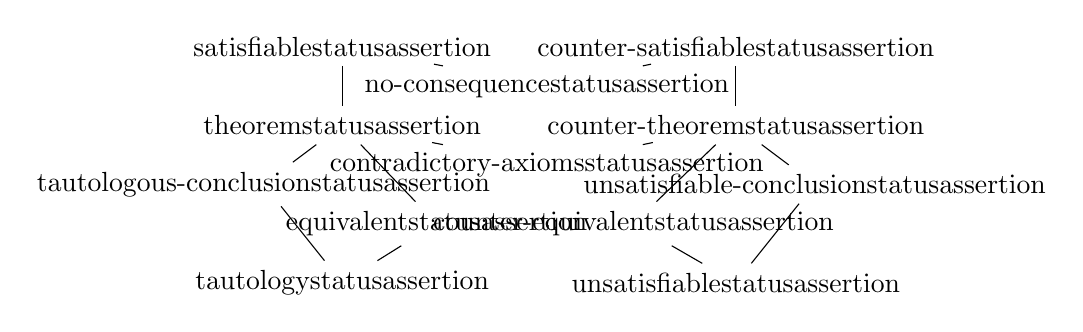
\begin{tikzpicture}
    \node (sat) at (1,4) {\attval{satisfiable}{status}{assertion}};
    \node (csat) at (6,4) {\attval{counter-satisfiable}{status}{assertion}};
    \node (thm) at (1,3) {\attval{theorem}{status}{assertion}};
    \node (cthm) at (6,3) {\attval{counter-theorem}{status}{assertion}};
    \node (tcon) at (0,2.25) {\attval{tautologous-conclusion}{status}{assertion}};
    \node (eqv) at (2.2,1.75) {\attval{equivalent}{status}{assertion}};
    \node (noc) at (3.6,3.5) {\attval{no-consequence}{status}{assertion}};
    \node (cax) at (3.6,2.5) {\attval{contradictory-axioms}{status}{assertion}};
    \node (ceqv) at (4.7,1.75) {\attval{counter-equivalent}{status}{assertion}};
    \node (ucon) at (7,2.25) {\attval{unsatisfiable-conclusion}{status}{assertion}};
    \node (taut) at (1,1) {\attval{tautology}{status}{assertion}};
    \node (usat) at (6,1) {\attval{unsatisfiable}{status}{assertion}};
    \draw (sat) -- (noc);
    \draw (sat) -- (thm);
    \draw (csat) -- (noc);
    \draw (csat) -- (cthm);
    \draw (thm) -- (tcon);
    \draw (thm) -- (cax);
    \draw (cthm) -- (cax);
    \draw (thm) -- (eqv);
    \draw (cthm) -- (ucon);
    \draw (cthm) -- (ceqv);
    \draw (tcon) -- (taut);
    \draw (eqv) -- (taut);
    \draw (ucon) -- (usat);
    \draw (ceqv) -- (usat);
  \end{tikzpicture}}
\end{myfig}
\end{tsubsection}

\begin{tsubsection}[id=type-assertions]{Type Assertions}
  In the last section, we have discussed the {\element{type}} elements in
  {\element{symbol}} declarations. These were axiomatic (and thus
  {\indextoo{theory-constitutive}}) in character, declaring a symbol to be of a certain
  type, which makes this information available to type checkers that can check
  well-typedness (and thus plausibility) of the represented mathematical objects.

  However, not all type information is axiomatic, it can also be deduced from other
  sources knowledge. We use the same {\element{type}} element we have discussed in
  {\mysubsecref{type-axioms}} for such {\twindef{type}{assertions}}, i.e. non-constitutive
  statements that inform a type-checker. In this case, the {\element{type}} element can
  occur at top level, and even outside a {\element{theory}} element (in which case they
  have to specify their home theory in the {\attribute{theory}{type}} attribute). 
  
  {\Mylstref{term-declaration}} contains a type assertion $x+x\colon evens$, which makes
  the information that doubling an integer number results in an even number available to
  the reasoning process.

\begin{lstlisting}[label=lst:term-declaration,
  caption={A Term declaration in {\omdoc}.},
  index={type,assertion}]
<type xml:id="double-even.td" system="#POST" 
      theory="adv.int" for="plus" just-by="#double-even">
  <m:math>
    <m:apply><m:plus/>
      <m:ci type="integer">X</m:ci>
      <m:ci type="integer">X</m:ci>
    </m:apply>
  </m:math>
  <m:math>
    <m:csymbol definitionURL="http://omdoc.org/cd/integers/evens"/>
  </m:math>
</type>

<assertion xml:id="double-even" type="lemma" theory="adv.int">
  <FMP>
    <m:math>
      <m:apply><m:forall/>
        <m:bvar><m:ci xml:id="x13" type="integer">X</m:ci></m:bvar>
        <m:apply><m:in/>
          <m:apply><m:plus/>
            <m:ci definitionURL="x13" type="integer">X</m:ci>
            <m:ci definitionURL="x13" type="integer">X</m:ci>
          </m:apply>
          <m:csymbol definitionURL="http://omdoc.org/cd/nat/evens"/>
        </m:apply>
      </m:apply>
    </m:math>
  </FMP>
</assertion>
\end{lstlisting}
The body of a type assertion contains two mathematical objects, first the type of
the object and the second one is the object that is asserted to have this
type.
\end{tsubsection}

\begin{tsubsection}[id=alternative]{Alternative Definitions}
  
  In contrast to what we have said about {\twintoo{conservative}{extension}s} at the end
  of {\mysubsecref{definitions}}, mathematical documents often contain multiple
  definitions for a concept or mathematical object. However, if they do, they also contain
  a careful analysis of equivalence among them. {\omdoc} allows us to model this by
  providing the {\eldef{alternative}} element.  Conceptually, an alternative definition or
  axiom is just a group of assertions that specify the equivalence of logical formulae. Of
  course, alternatives can only be added in a consistent way to a body of mathematical
  knowledge, if it is guaranteed that it is equivalent to the existing ones.  The
  {\attribute{for}{alternative}} on the {\element{alternative }} points to the symbol to
  which the alternative definition pertains.  Therefore, {\element{alternative}} has the
  attributes {\attribute{entails}{alternative}} and
  {\attribute{entailed-by}{alternative}}, that specify {\element{assertion}s} that state
  the necessary entailments. It is an {\indextoo{integrity condition}} of {\omdoc} that
  any {\element{alternative}} element references at least one {\element{definition}} or
  {\element{alternative}} element that entails it and one that it is entailed by (more can
  be given for convenience). The {\attribute{entails-thm}{alternative}}, and
  {\attribute{entailed-by-thm}{alternative}} attributes specify the corresponding
  assertions. This way we can always reconstruct equivalence of all definitions for a
  given symbol. As alternative definitions are not theory-constitutive, they can appear
  outside a {\element{theory}} element as long as they have a
  {\attribute{theory}{alternative}} attribute.
\end{tsubsection}

\begin{tsubsection}[id=assertional-statements,short=Assertional Statements]{Assertional Statements}
           
  There is another distinction for statements that we will need in the following. Some
  kinds of mathematical statements add information about the mathematical objects in
  question, whereas other statements do not. For instance, a symbol declaration only
  declares an unambiguous name for an object. We will call the following {\omdoc} elements
  {\defemph{assertional}\twin{assertional}{element}}: {\element{axiom}} (it asserts
  central properties about an object), {\element{type}} (it asserts type properties about
  an object), {\element{definition}} (this asserts properties of a new object), and of
  course {\element{assertion}}.
  
  The following elements are considered non-assertional: {\element{symbol}} (only a name
  is declared for an object), {\element{alternative}} (here the assertional content is
  carried by the {\element{assertion}} elements referenced in the structure-carrying
  attributes of {\element{alternative}}).  For the elements introduced below we will
  discuss whether they are assertional or not in their context. In a nutshell, only
  statements introduced by the module {\ADTmodule{spec}} (see {\mychapref{adt}}) will be
  assertional.
\end{tsubsection}           
\end{tsection}

\begin{tsection}[id=examples]{Mathematical Examples in OMDoc}

  In mathematical practice examples play a great role, e.g. in concept formation as
  witnesses for definitions or as either supporting evidence, or as counter-examples for
  conjectures.  Therefore examples are given status as primary objects in {\omdoc}.
  Conceptually, we model an example $\cE$ as a pair $(\cW,\bA)$, where
  $\cW=(\cW_1,\ldots,\cW_n)$ is an $n$-tuple of mathematical objects and $\bA$ is an
  assertion. If $\cE$ is an example for a mathematical concept given as an {\omdoc} symbol
  $\bS$, then $\bA$ must be of the form $\bS(\cW_1,\ldots,\cW_n)$. \ednote {MK: Actually,
    an example is much better modelled as a view. we need to rework this section to
    conform better to this model. In the meantime we have extended the model of the
    example element to allow a morphism instead of the objects.}
  
  If $\cE$ is an example for a conjecture $\bC$, then we have to consider the situation
  more carefully.\ednote{MK: it is not clear to me yet, how this can be fitted into the
    view model yet. Need to think; interesting.} We assume that $\bC$ is of the form
  $\cQ\bD$ for some formula $\bD$, where $\cQ$ is a sequence $\cQ_1W_1,\ldots,\cQ_mW_m$ of
  $m\geq n=\#\cW$ quantifications of using quantifiers $\cQ_i$ like $\forall$ or
  $\exists$.  Now let $\cQ'$ be a sub-sequence of $m-n$ quantifiers of $\cQ$ and $\bD'$ be
  $\bD$ only that all the $W_{i_j}$ such that the $\cQ_{i_j}$ are absent from $\cQ'$ have
  been replaced by $\cW_j$ for $1\leq j\leq n$.  If $\cE=(\cW,\bA)$ supports $\bC$, then
  $\bA=\cQ'\bD'$ and if $\cE$ is a counter-example for $\bC$, then $\bA=\neg\cQ'\bD'$.
  
  {\omdoc} specifies this intuition in an {\eldef{example}} element that contains a
  multilingual {\element{CMP}} group\twin{multilingual}{group} for the description and $n$
  mathematical objects (the witnesses). It has the attributes
\begin{description}
\item[{\attribute{for}{example}}] specifying for which concepts or assertions it is an
  example.  This is a reference to a {\indextoo{whitespace-separated list}} of
  {\indextoo{URI}} references to {\element{symbol}}, {\element{definition}},
  {\element{axiom}}, {\element{alternative}}, or {\element{assertion}} elements.
\item[{\attribute{type}{example}}] specifying the aspect, the value is one of
  {\attval{for}{type}{example}} or {\attval{against}{type}{example}}
\item[{\attribute{assertion}{example}}] a reference to the assertion $\bA$
  mentioned above that formally states that the witnesses really form an example for the
  concept of assertion. In many cases even the statement of this is non-trivial
  and may require a proof.
\end{description}

{\element{example}} elements are considered non-assertional\twin{assertional}{element} in
{\omdoc}, since the assertional part is carried by the {\element{assertion}} element
referenced in the {\attribute{assertion}{example}} attribute.

Note that the list of mathematical objects in an {\element{example}} element does not
represent multiple examples, but corresponds to the argument list of the symbol, they
exemplify. In the example below, the symbol for monoid is a three-place relation (see the
type declaration in {\mylstref{symbol}}), so we have three witnesses.

\begin{lstlisting}[label=lst:example,mathescape,
  caption={An {\omdoc} representation of a mathematical example},
  index={example,for,type,assertion}]
<symbol name="strings-over"/>
<definition xml:id="strings.def" for="strings-over">$\ldots$ $A^*$ $\ldots$</definition>
<symbol name="concat"/>
<definition xml:id="concat.def" for="concat">$\ldots$ $::$ $\ldots$</definition>
<symbol name="empty-string"/>
<definition xml:id="empty-string.def" for="empty-string">$\ldots$ $\epsilon$ $\ldots$</definition>
$\ldots$
<assertion xml:id="string.struct.monoid" type="lemma">
  <CMP><xhtml:p>$(A^*,::,\epsilon)$ is a monoid.</xhtml:p></CMP>
  <FMP>$mon(A^*,::,\epsilon)$</FMP>
</assertion>
$\ldots$
<example xml:id="mon.ex1" for="monoid" type="for"
        assertion="string.struct.monoid">
  <CMP><xhtml:p>The set of strings with concatenation is a monoid.</xhtml:p></CMP>
  <OMOBJ>
    <OMA id="nat-strings">
      <OMS cd="strings" name="strings"/>
      <OMS cd="setname1" name="N"/>
    </OMA>
  </OMOBJ>
  <OMOBJ><OMS cd="strings" name="concat"/></OMOBJ>
  <OMOBJ><OMS cd="strings" name="empty-string"/></OMOBJ>
</example>

<assertion xml:id="monoid.are.groups" type="false-conjecture">
 <CMP><xhtml:p>Monoids are groups.</xhtml:p></CMP>
 <FMP>$\allcdot{S,o,e}{mon(S,o,e)\rightarrow\excdot{i}{group(S,o,e,i)}}$</FMP>
</assertion>

<example xml:id="mon.ex2" for="#monoids.are.groups" type="against"
        assertion="strings.isnt.group">
  <CMP><xhtml:p>The set of strings with concatenation is not a group.</xhtml:p></CMP>
  <OMOBJ><OMR href="#nat-strings"/></OMOBJ>
  <OMOBJ><OMS cd="strings" name="strings"/></OMOBJ>
  <OMOBJ><OMS cd="strings" name="concat"/></OMOBJ>
  <OMOBJ><OMS cd="strings" name="empty-string"/></OMOBJ>
</example>

<assertion xml:id="strings.isnt.group" type="theorem">
  <CMP><xhtml:p>$(A^*,::,\epsilon)$ is a monoid, but there is no inverse function for it.</xhtml:p></CMP>
</assertion>
\end{lstlisting}

In {\mylstref{example}} we show an example of the usage of an {\element{example}} element
in {\omdoc}: We declare constructor symbols {\snippet{strings-over}}, that takes an
{\indextoo{alphabet}} $A$ as an argument and returns the set $A^*$ of
{\indextoo{strings}s} over $A$, {\snippet{concat}} for {\twintoo{strings}{concatenation}}
(which we will denote by $::$), and {\snippet{empty-string}} for the
{\twintoo{empty}{string}} $\epsilon$.  Then we state that $\cW=(A^*,::,\epsilon)$ is a
monoid in an {\element{assertion}} with {\snippet{xml:id="string.struct.monoid"}}.  The
{\element{example}} element with {\snippet{xml:id="mon.ex1"}} in {\mylstref{example}} is
an example for the concept of a monoid, since it encodes the pair $(\cW,\bA)$ where $\bA$
is given by reference to the assertion {\snippet{string.struct.monoid}} in the
{\attribute{assertion}{example}} attribute.  Example {\snippet{mon.ex2}} uses the pair
$(\cW,\bA')$ as a {\indextoo{counter-example}} to the {\twintoo{false}{conjecture}}
{\snippet{monoids.are.groups}} using the assertion {\snippet{strings.isnt.group}} for
$\bA'$.
\end{tsection}

\begin{tsection}[id=inline-statements]{Inline Statements}

  Note that the infrastructure for statements introduced so far does its best to mark up
  the interplay of formal and informal elements in mathematical documents, and make
  explicit the influence of the context and their contribution to it. However, not all
  statements in mathematical documents can be adequately captured directly.  Consider for
  instance the following situation, which we might find in a typical mathematical
  textbook.
\begin{quote}
  {\bf{Theorem 3.12}}: {\emph{In a monoid $M$ the left unit and the right unit coincide,
      we call it the {\bf{unit}} of $M$.}}
\end{quote}
The overt role of this text fragment is that of a mathematical theorem --- as indicated by
the cue word ``{\bf{Theorem}}'', therefore we would be tempted represent it as an
{\element{omtext}} element with the value {\attval{theorem}{type}{attribute}} for the
{\attribute{type}{attribute}} attribute. But the relative clause is clearly a
{\indextoo{definition}} (the {\indextoo{definiens}} is even marked in boldface). What we
have here is an aggregated verbalization of two mathematical statements. In a simple case
like this one, we could represent this as follows:

\begin{lstlisting}[mathescape,caption=A Simple-Minded Representation of {\bf{Theorem 3.12}}]
<assertion type="theorem" style="display=flow">
  <CMP><xhtml:p>In a monoid $M$, the left unit and the right unit coincide,</xhtml:p></CMP>
</assertion>
<definition for="unit" style="display:flow">
   <CMP><xhtml:p>we call it the <term role="definiendum" name="unit">unit</term> of $M$</xhtml:p></CMP>
</definition>
\end{lstlisting}

But this representation remains unsatisfactory: the definition is not part of the theorem,
which would really make a difference if the theorem continued after the inline
definition. The real problem is that the inline definition is linguistically a
phrase-level construct, while the {\element{omtext}} element is a discourse-level
construct. However, as a phrase-level construct, the inline definition cannot really be
gren the context it is presented in (which is the
beauty of it; the re-use of context). With the {\element{phrase}} element and its
\attributeshort{verbalizes}, we can do the following:

\begin{lstlisting}[mathescape,caption=An Inline Definition]
<assertion xml:id='unit-unique' type="theorem" >
  <CMP><xhtml:p>In a monoid M, the left unit and the right unit coincide,
    <xhtml:span verbalizes="#unit-def">we call it the unit of M</xhtml:span>.</xhtml:p></CMP>
</assertion>
<symbol name="unit"/>
<definition xml:id="unit-def" for="unit" just-by='#unit-unique'>
  <CMP><xhtml:p>We call the (unique) element of a monoid M that acts as a left 
    and right unit the <term role="definiendum" name="unit">unit</term> of M.</xhtml:p></CMP>
</definition>
\end{lstlisting}

thus we would have the phrase-level markup in the proper place, and we would have an
explicit version of the definition which is standalone\footnote{Purists could use the CSS
  attribute {\attribute{style}{definition}} on the {\element{definition}} element with
  value {\attvalshort{display:none}{style}} to hides it from the document; it might also
  be placed into another document altogether}, and we would have the explicit relation
that states that the inline definition is an ``abbreviation'' of the standalone
definition.
\end{tsection}

\begin{tsection}[id=theories]{Theories as Structured Contexts}

  {\omdoc} provides an infrastructure for mathematical theories as first-class objects
  that can be used to structure larger bodies of mathematics by functional aspects, to
  serve as a framework for semantically referencing mathematical objects, and to make
  parts of mathematical developments reusable in multiple contexts. The module
  {\STmodule{spec}} presented in this chapter introduces a part of this infrastructure,
  which can already address the first two concerns. For the latter, we need the machinery
  for complex theories introduced in {\mychapref{complex-theories}}.

  Theories are specified by the {\eldef{theory}} element in {\omdoc}, which has an
  optional {\attribute[ns-attr=xml]{id}{theory}} attribute for referencing the
  theory. Furthermore, the {\element{theory}} element can have the
  {\attribute[ns-elt=om]{cdbase}{theory}} attribute that allows to specify the
  {\attribute{cdbase}{OMS}} this theory uses for disambiguation on
  {\element[ns-elt=om]{OMS}} elements (see {\mysecref{openmath}} for a discussion).
  Additional information about the theory like a title or a short description can be given
  in the {\element{metadata}} element. After this, any {\indextoo{top-level}} {\omdoc}
  element can occur, including the theory-constitutive elements introduced in
  {\mysecsref{statements-constitutive}{definitions}}, even {\element{theory}} elements
  themselves. Note that theory-constitutive elements may {\emph{only}} occur in
  {\element{theory}} elements.

  Note that theories can be structured like documents e.g. into sections and the like (see
  {\mysecref{sectioning}} for a discussion) via the {\eldef{omgroup}} element.

\begin{myfig}{simple-thy}{Theories in {\omdoc}}
\begin{scriptsize}
\begin{tabular}{|>{\tt}l|>{\tt}l|>{\tt}p{5.4truecm}|c|>{\tt}p{2truecm}|}\hline
{\rm Element}& \multicolumn{2}{l|}{Attributes\hspace*{2.25cm}} & D & Content  \\\hline
             & {\rm Req.}  & {\rm Optional}                & C &           \\\hline\hline
 theory      &                 & xml:id, class, style, cdbase, 
                                 cdversion, cdrevision, cdstatus, cdurl, 
                                 cdreviewdate          & + & (\llquote{top+thc} | imports)*\\\hline
 imports     & from            & id, type, class, style        & + & \\\hline
\multicolumn{5}{|p{11cm}|}{where \llquote{top+thc} stands for top-level and
  theory-constitutive elements}\\\hline
\end{tabular}
\end{scriptsize}
\end{myfig}

\begin{tsubsection}[id=inheritance]{Simple Inheritance}

{\element{theory}} elements can contain {\element{imports}} elements (mixed in
with the top-level ones) to specify inheritance: The main idea behind structured theories
and specification is that not all theory-constitutive elements need to be explicitly
stated in a theory; they can be inherited from other theories. Formally, the set of
theory-constitutive elements in a theory is the union of those that are explicitly
specified and those that are imported from other theories. This has consequences later on,
for instance, these are available for use in proofs. See
{\mysecref{proofs:justifications}} for details on availability of assertional statements in
proofs and justifications.

The meaning of the {\eldef{imports}} element is determined by two attributes:
\begin{description}
\item[{\attribute{from}{imports}}] The value of this attribute is a
  {\twintoo{URI}{reference}} that specifies the {\twindef{source}{theory}}, i.e. the
  theory we import from.  The current theory (the one specified in the parent of the
  {\element{imports}} element, we will call it the {\twindef{target}{theory}}) inherits
  the constitutive elements from the source theory.
\item[{\attribute{type}{imports}}] This optional attribute can have the values
  {\attval{global}{type}{imports}} and {\attval{local}{type}{imports}} (the former is
  assumed, if the attribute is absent): We call constitutive elements {\defin{local}} to
  the current theory, if they are explicitly defined as children, and else
  {\defin{inherited}}. A {\twindef{local}{import}} (an {\element{imports}} element with
  {\snippet{type="local"}}) only imports the local elements of the source theory, a
  {\indextoo{global}} import also the inherited ones.
\end{description}
  The meaning of nested {\element{theory}} elements is given in terms of an
  implicit imports relation: The inner theory imports from the outer one. Thus
\begin{lstlisting}[label=lst:nested-thy,index={theory}]
<theory xml:id="a.thy">
  <symbol name="aa"/>
  <theory xml:id="b.thy">
    <symbol name="cc"/>
    <definition xml:id="cc.def" for="cc" type="simple">
       <OMOBJ><OMS cd="a.thy" name="aa"/></OMOBJ>
    </definition>
  </theory>
</theory>
\end{lstlisting}
is equivalent to 
\begin{lstlisting}[label=lst:nested-thy-equiv,index={theory}]
<theory xml:id="a.thy"><symbol name="aa"/></theory>
<theory xml:id="b.thy">
  <imports from="#a.thy" type="global"/>
  <symbol name="cc"/>
  <definition xml:id="cc.def" for="cc" type="simple">
     <OMOBJ><OMS cd="a.thy" name="aa"/></OMOBJ>
  </definition>
</theory>
\end{lstlisting}
In particular, the symbol {\snippet{cc}} is visible only in theory {\snippet{b.thy}}, not
in the rest of theory {\snippet{a.thy}} in the first representation.  Note that the
inherited elements of the current theory can themselves be inherited in the source
theory. For instance, in the {\mylstref{def-group}} the {\snippet{left-inv}} is the only
local axiom of the theory {\snippetin{group}}, which has the inherited axioms
{\snippet{closed}}, {\snippet{assoc}}, {\snippet{left-unit}}.

In order for this import mechanism to work properly, the
{\twintoo{inheritance}{relation}}, i.e.  the relation on theories induced by the
{\element{imports}} elements, must be {\indextoo{acyclic}}. There is another, more subtle
constraint on the inheritance relation concerning multiple inheritance.  Consider the
situation in {\mylstref{multiple-inheritance}}: here theories {\snippet{A}} and
{\snippet{B}} import theories with {\snippet{xml:id="mythy"}}, but from different
URIs. Thus we have no guarantee that the theories are identical, and semantic integrity of
the theory {\snippet{C}} is at risk. Note that this situation might in fact be totally
unproblematic, e.g. if both URIs point to the same document, or if the referenced
documents are identical or equivalent. But we cannot guarantee this by content markup
alone, we have to forbid it to be safe.

\begin{lstlisting}[label=lst:multiple-inheritance,
  caption={Problematic Multiple Inheritance},
  index={theory,symbol,axiom,imports}]
<theory xml:id="A">
  <imports from="http://red.com/theories.omdoc#mythy"/>
</theory>
<theory xml:id="B">
  <imports from="http://blue.org/cd/all.omdoc#mythy"/>
</theory>
<theory xml:id="C"><imports from="#A"/><imports from="#B"/></theory>
\end{lstlisting}

Let us now formulate the constraint carefully, the {\twindef{base}{URI}} of an {\xml}
document is the {\indextoo{URI}} that has been used to retrieve it.  We adapt this to
{\omdoc} theory elements: the base URI of an imported theory is the URI declared in the
{\attribute{cdbase}{theory}} attribute of the {\element{theory}} element (if present) or
the base URI of the document which contains it\footnote{Note that the base URI of the
  document is sufficient, since a valid {\omdoc} document cannot contain more than one
  {\element{theory}} element for a given {\attribute[ns-attr=xml]{id}{theory}}}. For
theories that are imported along a chain of global imports, which include
{\twintoo{relative}{URI}s}, we need to employ {\twintoo{URI}{normalization}} to compute
the {\twintoo{effective}{URI}}.  Now the constraint is that any two imported theories that
have the same value of the {\attribute[ns-attr=xml]{id}{theory}} attribute must have the
same base URI. Note that this does not imply a global unicity constraint for
{\attribute[ns-attr=xml]{id}{theory}} values of {\element{theory}} elements, it only means
that the mapping of theory identifiers to URIs is unambiguous in the dependency cone of a
theory.

In {\mylstref{def-group}} we have specified three algebraic theories that gradually build
up a theory of groups importing theory-constitutive statements (symbols, axioms, and
definitions) from earlier theories and adding their own content. The theory
{\snippetin{semigroup}} provides symbols for an operation {\snippetin{op}} on a base set
{\snippetin{set}} and has the axioms for closure and associativity of
{\snippetin{op}}. The theory of monoids imports these without modification and uses them
to state the {\snippet{left-unit}} axiom. The theory {\snippetin{monoid}} then proceeds to
add a symbol {\snippetin{neut}} and an axiom that states that it acts as a left unit with
respect to {\snippetin{set}} and {\snippetin{op}}.  The theory {\snippetin{group}}
continues this process by adding a symbol {\snippetin{inv}} for the function that gives
inverses and an axiom that states its meaning.

\begin{lstlisting}[label=lst:def-group,escapechar=\%,mathescape,
  caption={A Structured Development of Algebraic Theories in {\omdoc}},
  index={theory,symbol,axiom,imports}]
<theory xml:id="semigroup">
  <symbol name="set"/><symbol name="op"/>
  <axiom xml:id="closed"> $\ldots$ </axiom><axiom xml:id="assoc"> $\ldots$ </axiom>
</theory>

<theory xml:id="monoid">
  <imports from="#semigroup"/>
  <symbol name="neut"/><symbol name="setstar"/>
  <axiom xml:id="left-unit">
    <CMP><xhtml:p>%\tt{neut}% is a left unit for %\tt{op}%.</xhtml:p></CMP><FMP>$\allcdot{x\in{\tt{set}}}{{\tt{op}}(x,{\tt{neut}})=x}$</FMP>
  </axiom>
  <definition xml:id="setstar.def" for="setstar" type="implicit">
    <CMP><xhtml:p>$\cdot^*$ subtracts the unit from a set </xhtml:p></CMP><FMP>$\allcdot{S}{S^*=S\backslash\set{\tt{unit}}}$</FMP>
  </definition>
</theory>

<theory xml:id="group"> 
  <imports from="#monoid"/>
  <symbol name="inv"/>
  <axiom xml:id="left-inv">
    <CMP><xhtml:p>For every $X\in\tt{set}$ there is an inverse ${\tt{inv}}(X)$ wrt. %\tt{op}%.</xhtml:p></CMP>
  </axiom>
</theory>
\end{lstlisting}

The example in {\mylstref{def-group}} shows that with the notion of theory inheritance it
is possible to re-use parts of theories and add structure to specifications. For instance
it would be very simple to define a theory of {\twintoo{Abelian}{semigroup}s} by adding a
{\twintoo{commutativity}{axiom}}.

The set of symbols, axioms, and definitions available for use in proofs in the importing
theory consists of the ones directly specified as {\element{symbol}}, {\element{axiom}},
and {\element{definition}} elements in the target theory itself (we speak of
{\defin{local}} axioms and definitions in this case) and the ones that are inherited from
the source theories via {\element{imports}} elements.  Note that these symbols, axioms,
and definitions (we call them {\defin{inherited}}) can consist of the local ones in the
source theories and the ones that are inherited there.

The local and inherited symbols, definitions, and axioms are the only ones
available to mathematical statements and proofs. If a symbol is not available in
the home theory (the one given by the dominating {\element{theory}} element or the
one specified in the {\attribute{theory}{statement}} attribute of the statement),
then it cannot be used since its semantics is not defined.
\end{tsubsection}

\begin{tsubsection}[id=identifying]{OMDoc Theories as Content Dictionaries}
  
  In {\mychapref{mobj}}, we have introduced the {\openmath} and {\cmathml} representations
  for mathematical objects and formulae. One of the central concepts there was the notion
  that the representation of a symbol includes a pointer to a document that defines its
  meaning. In the original {\openmath} standard, these documents are identified as
  {\openmath} content dictionaries\index{content dictionary!OpenMath}, the {\mathml}
  recommendation is not specific. In the examples above, we have seen that {\omdoc}
  documents can contain definitions of mathematical concepts and symbols, thus they are
  also candidates for ``defining documents'' for symbols.  By the {\openmath}2
  standard~\cite{BusCapCar:2oms04} suitable classes of {\omdoc} documents can act as
  {\openmath} content dictionaries (we call them {\defemph{{\omdoc} content
      dictionaries}}\twin{content dictionary}{OMDoc}; see
  {\mysubsecref{sub-languages:cd}}).  The main distinguishing feature of {\omdoc} content
  dictionaries is that they include {\element{theory}} elements with
  {\twintoo{symbol}{declaration}s} (see {\mysecref{definitions}}) that act as the targets
  for the pointers in the symbol representations in {\openmath} and {\cmathml}. The theory
  name specified in the {\attribute[ns-attr=xml]{id}{theory}} attribute of the
  {\element{theory}} element takes the place of the {\snippet{CDname}} defined in the
  {\openmath} content dictionary\index{content dictionary!OpenMath}.
  
  Furthermore, the {\indextoo{URI}} specified in the {\attribute{cdbase}{theory}}
  attribute is the one used for disambiguation on {\element[ns-elt=om]{OMS}} elements (see
  {\mysecref{openmath}} for a discussion).
  
  For instance the symbol declaration in {\mylstref{symbol}} can be referenced as
\begin{lstlisting}
<OMS cd="elAlg" name="monoid" cdbase="http://omdoc.org/algebra.omdoc"/>
\end{lstlisting}
if it occurs in a theory for elementary algebra whose
{\attribute[ns-attr=xml]{id}{theory}} attribute has the value {\snippet{elAlg}} and which
occurs in a resource with the URI \url{http://omdoc.org/algebra.omdoc} or if the
{\attribute{cdbase}{theory}} attribute of the {\element{theory}} element has the value
\url{http://omdoc.org/algebra.omdoc}.


To be able to act as an {\openmath}2 {\twintoo{content dictionary}{format}}, {\omdoc} must
be able to express {\twintoo{content dictionary}{metadata}} (see {\mylstref{omcd}} for an
example). For this, the {\element{theory}} element carries some optional attributes that
allow to specify the administrative metadata of {\openmath} content dictionaries.

The {\attribute{cdstatus}{theory}} attribute specifies the {\twindef{content
    dictionary}{status}}, which can take one of the following values:
{\attval{official}{cdstatus}{theory}} (i.e. approved by the {\openmath} Society),
{\attval{experimental}{cdstatus}{theory}} (i.e. under development and thus liable to
change), {\attval{private}{cdstatus}{theory}} (i.e. used by a private group of {\openmath}
users) or {\attval{obsolete}{cdstatus}{theory}} (i.e. only for archival purposes). The
attributes {\attribute{cdversion}{theory}} and {\attribute{cdrevision}{theory}} jointly
specify the {\twindef{content dictionary}{version number}}, which consists of two parts, a
major {\defin{version}} and a {\defin{revision}}, both of which are non-negative
integers. For details between the relation between content dictionary status and versions
consult the {\openmath} standard~\cite{BusCapCar:2oms04}.

Furthermore, the {\element{theory}} element can have the following attributes:
\begin{description}
\item[\attribute{cdbase}{theory}] for the {\twintoo{content dictionary}{base}} which, when
  combined with the content dictionary name, forms a unique identifier for the content
  dictionary. It may or may not refer to an actual location from which it can be
  retrieved.
\item[\attribute{cdurl}{theory}] for a valid URL where the source file for the content
  dictionary encoding can be found.
\item[\attribute{cdreviewdate}{theory}] for the {\twindef{review}{date}} of the content
  dictionary, i.e. the date until which the content dictionary is guaranteed to remain
  unchanged.
\end{description}
\end{tsubsection}

\end{tsection}
\end{tchapter}

%%% Local Variables: 
%%% mode: latex
%%% TeX-master: "omdoc"
%%% End: 

% LocalWords:  lang adt lst mathescape en monoide mon qtconst def cd dc cmp om
% LocalWords:  nat eq xref int suc requation exp rec ref qttheory sst dec csat
% LocalWords:  isnt peano ness bvar mtext concat empystrg setname OMR xlink Ai
% LocalWords:  href Luehts MMiSS qaulified mythy Bi CiA CiB escapechar setstar
% LocalWords:  gim mobj CDname elAlg es td adv ci csymbol definitionURL aa cc
% LocalWords:  equiv cdbase openmath ns elt attr cdversion FMP pres af
% LocalWords:  cdrevision cdstatus cdurl cdreviewdate OMBIND OMATTR multi bool
% LocalWords:  metadata OMOBJ arities OMA sgrp forall thm mW inv Req wrt omcd
% LocalWords:  nmueller ple Inline omtext cthm tcon eqv noc cax ceqv ucon usat
% LocalWords:  omgroup thc

%%%%%%%%%%%%%%%%%%%%%%%%%%%%%%%%%%%%%%%%%%%%%%%%%%%%%%%%%%%%%%%%%%%%%%%%%
% This file is part of the LaTeX sources of the OMDoc 1.3 specification
% Copyright (c) 2016 Michael Kohlhase.
% Source at https://github.com/KWARC/OMDoc/tree/master/doc/spec
% This work is licensed by the Creative Commons Share-Alike license
% see http://creativecommons.org/licenses/by-sa/2.5/ for details
%%%%%%%%%%%%%%%%%%%%%%%%%%%%%%%%%%%%%%%%%%%%%%%%%%%%%%%%%%%%%%%%%%%%%%%%%

\begin{tchapter}[id=adt,short=Abstract Data Types]{Abstract Data Types (Module {\ADTmodule{spec}})}

  Most specification languages for mathematical theories support definition mechanisms for
  sets that are inductively generated by a set of constructors and
  {\twintoo{recursive}{function}s} on these under the heading of {\twindef{abstract}{data
      type}s}. Prominent examples of abstract data types are natural numbers, lists,
  trees, etc. The module {\ADTmodule{spec}} presented in this chapter extends {\omdoc} by
  a concise syntax for abstract data types that follows the model used in the {\casl}
  (Common Abstract Specification Language~\cite{CoFI:2004:CASL-RM}) standard.

  Conceptually, an abstract data type declares a collection of symbols and axioms that can
  be used to construct certain mathematical objects and to group them into sets. For
  instance, the {\twintoo{Peano}{axioms}} (see {\myfigref{peano}}) introduce the symbols
  $0$ (the number {\indextoo{zero}}), $s$ (the {\twintoo{successor}{function}}), and $\NN$
  (the set of {\twintoo{natural}{number}s}) and fix their meaning by five axioms. These
  state that the set $\NN$ contains exactly those objects that can be constructed from $0$
  and $s$ alone (these symbols are called {\twindef{constructor}{symbol}s} and the
  representations {\twindef{constructor}{term}s}). Optionally, an abstract data type can
  also declare {\twindef{selector}{symbol}s}, for (partial) inverses of the
  constructors. In the case of natural numbers the {\twintoo{predecessor}{function}} is a
  selector for $s$: it ``selects'' the argument $n$, from which a (non-zero) number $s(n)$
  has been constructed.

  Following {\casl} we will call sets of objects that can be represented as constructor
  terms {\defin{sort}s}. A sort is called {\defin{free}}, iff there are no identities
  between constructor terms, i.e.  two objects represented by different constructor terms
  can never be equal. The sort $\NN$ of natural numbers is a free sort. An example of a
  sort that is not free is the theory of finite sets given by the constructors $\emptyset$
  and the {\twintoo{set}{insertion}} function $\iota$ , since the set $\{a\}$ can be
  obtained by inserting $a$ into the empty set an arbitrary (positive) number of times; so
  e.g. $\iota(a,\emptyset)=\iota(a,\iota(a,\emptyset))$. This kind of sort is called
  {\defin{generated}}, since it only contains elements that are expressible in the
  constructors. An abstract data type is called {\defin{loose}}, if it contains elements
  besides the ones generated by the constructors. We consider free sorts more
  {\defin{strict}} than generated ones, which in turn are more strict than loose ones.
\begin{myfig}{adtheory}{Abstract data types in {\omdoc}}
\scriptsize
\begin{tabular}{|>{\tt}l|>{\tt}l|>{\tt}p{3.3truecm}|c|>{\tt}p{3truecm}|}\hline
{\rm Element}& \multicolumn{2}{l|}{Attributes\hspace*{2.25cm}} & D & Content  \\\hline
             & {\rm Req.}  & {\rm Optional}     & C &           \\\hline\hline
 adt         &          & xml:id, class, style, parameters  & +  & sortdef+\\\hline
 sortdef     & name     & type, role, scope, class, style & + & (constructor | insort)*, recognizer? \\\hline
 constructor & name     & type, scope, class, style & +  & argument*\\\hline
 argument    &          &              & +  & type, selector?\\\hline
 insort      & for      &              & -- & \\\hline
 selector    & name     & type, scope, role, total, class, style
                                       & + & EMPTY\\\hline
 recognizer  & name     & type, scope, role, class, style & + & \\\hline
\end{tabular}
\end{myfig}

\noindent In {\omdoc}, we use the {\eldef{adt}} element to specify
abstract data types possibly consisting of multiple sorts.  It is a
{\indextoo{theory-constitutive}} statement and can only occur as a
child of a {\element{theory}} element (see
{\mysecref{statements-constitutive}} for a discussion). An
{\element{adt}} element contains one or more {\element{sortdef}}
elements that define the {\indextoo{sort}s} and specify their
members and it can carry a {\attribute{parameters}{adt}} attribute
that contains a whitespace-separated list of parameter variable
names. If these are present, they declare type variables that can be
used in the specification of the new sort and constructor symbols
see {\mysecref{verifun}} for an example.

We will use an augmented representation of the abstract data type of natural numbers as a
running example for introduction of the functionality added by the {\ADTmodule{spec}}
module; {\mylstref{nat-adt}} contains the listing of the {\omdoc} encoding. In this
example, we introduce a second sort $\bbP$ for {\atwintoo{positive}{natural}{number}s} to
make it more interesting and to pin down the {\indextoo{type}} of the
{\twintoo{predecessor}{function}}.

A {\eldef{sortdef}} element is a highly condensed piece of syntax that declares a
{\twintoo{sort}{symbol}} together with the {\twintoo{constructor}{symbol}s} and their
{\twintoo{selector}{symbol}s} of the corresponding sort. It has a required
{\attribute{name}{sortdef}} attribute that specifies the symbol name, an optional
{\attribute{type}{adt}} attribute that can have the values {\attval{free}{type}{adt}},
{\attval{generated}{type}{adt}}, and {\attval{loose}{type}{adt}} with the meaning
discussed above. A {\element{sortdef}} element contains a set of {\eldef{constructor}} and
{\eldef{insort}} elements.  The latter are empty elements which refer to a sort declared
elsewhere in a {\element{sortdef}} with their {\attribute{for}{insort}} attribute: An
{\element{insort}} element with
{\snippet{for="}}\llquote{URI}{\snippet{\#\llquote{name}"}} specifies that all the
constructors of the sort {\snippet{\llquote{name}}} are also constructors for the one
defined in the parent {\element{sortdef}}.  Furthermore, the type of a sort given by a
{\element{sortdef}} element can only be as strict as the types of any sorts included by
its {\element{insort}} children.

{\Mylstref{nat-adt}} introduces the {\twintoo{sort}{symbol}s} {\snippet{pos-nats}}
(positive natural numbers) and {\snippet{nats}} (natural numbers) , the symbol names are
given by the required {\attribute{name}{constructor}} attribute. Since a constructor is in
general an $n$-ary function, a {\element{constructor}} element contains $n$
{\eldef{argument}} children that specify the argument sorts of this function along with
possible selector functions. The argument sort is given as the first child of the
{\element{argument}} element: a {\element{type}} element as described in
{\mysubsecref{type-axioms}}.  Note that $n$ may be 0 and thus the constructor element may not
have {\element{argument}} children (see for instance the {\element{constructor}} for
{\snippet{zero}} in {\mylstref{nat-adt}}). The first {\element{sortdef}} element there
introduces the constructor symbol {\snippet{succ@Nat}} for the
{\twintoo{successor}{function}}. This function has one argument, which is a natural number
(i.e. a member of the sort {\snippet{nats}}).

Sometimes it is convenient to specify the inverses of a constructors that are
functions. For this {\omdoc} offers the possibility to add an empty {\eldef{selector}}
element as the second child of an {\element{argument}} child of a
{\element{constructor}}. The required attribute {\attribute{name}{selector}} specifies the
symbol name, the optional {\attribute{total}{selector}} attribute of the
{\element{selector}} element specifies whether the function represented by this symbol is
total\twin{total}{function} (value {\attval{yes}{total}{selector}}) or
partial\twin{partial}{function} (value {\attval{no}{total}{selector}}).  In
{\mylstref{nat-adt}} the {\element{selector}} element in the first {\element{sortdef}}
introduces a {\twintoo{selector}{symbol}} for the {\twintoo{successor}{function}}
{\snippet{succ}}. As {\snippet{succ}} is a function from {\snippet{nats}} to
{\snippet{pos-nats}}, {\snippet{pred}} is a total function from {\snippet{pos-nats}} to
{\snippet{nats}}.

Finally, a {\element{sortdef}} element can contain a {\eldef{recognizer}} child that
specifies a symbol for a {\indextoo{predicate}} that is true, iff its argument is of the
respective sort. The name of the predicate symbol is specified in the required
{\attribute{name}{recognizer}} attribute. {\Mylstref{nat-adt}} introduces such a
{\twindef{recognizer}{predicate}} as the last child of the {\element{sortdef}} element for
the sort {\snippet{pos-nats}}.

Note that the {\element{sortdef}}, {\element{constructor}}, {\element{selector}},
and {\element{recognizer}} elements define symbols of the name specified by their
{\attribute{name}{symbol}} element in the theory that contains the {\element{adt}}
element. To govern the visibility, they carry the attribute
{\attribute{scope}{symbol}} (with values {\attval{global}{scope}{symbol}} and
{\attval{local}{scope}{symbol}}) and the attribute {\attribute{role}{symbol}}
(with values {\attval{type}{role}{symbol}}, {\attval{sort}{role}{symbol}},
{\attval{object}{role}{symbol}}).
\begin{lstlisting}[label=lst:nat-adt,
  caption={The natural numbers using {\element{adt}} in {\omdoc}},
  index={adt,sortdef,constructor,argument,selector,recognizer,insort}]
<theory xml:id="Nat">
  <adt xml:id="nat-adt">
    <metadata>
      <dc:title>Natural Numbers as an Abstract Data Type.</dc:title>
      <dc:description>The Peano axiomatization of natural numbers.</dc:description>
    </metadata>

    <sortdef name="pos-nats" type="free">
      <metadata>
        <dc:description>The set of positive natural numbers.</dc:description>
      </metadata>
      <constructor name="succ">
        <metadata><dc:description>The successor function.</dc:description></metadata>
        <argument>
          <type><OMOBJ><OMS cd='Nat' name="nats"/></OMOBJ></type>
          <selector name="pred" total="yes">
            <metadata><dc:description>The predecessor function.</dc:description></metadata>
          </selector>
        </argument>
      </constructor>
      <recognizer name="positive">
        <metadata>
          <dc:description>
            The recognizer predicate for positive natural numbers.
          </dc:description>
        </metadata>
      </recognizer>
    </sortdef>

    <sortdef name="nats"  type="free">
      <metadata><dc:description>The set of natural numbers</dc:description></metadata>
      <constructor name="zero">
        <metadata><dc:description>The number zero.</dc:description></metadata>
      </constructor>
      <insort for="#pos-nats"/>
    </sortdef>
  </adt>
</theory>
\end{lstlisting}
To summarize {\mylstref{nat-adt}}: The abstract data type {\snippet{nat-adt}} is free and
defines two sorts {\snippet{pos-nats}} and {\snippet{nats}} for the (positive) natural
numbers. The positive numbers ({\snippet{pos-nats}}) are generated by the successor
function (which is a constructor) on the natural numbers (all positive natural numbers are
successors). On {\snippet{pos-nats}}, the inverse {\snippet{pred}} of {\snippet{succ}} is
{\indextoo{total}}.  The set {\snippet{nats}} of all natural numbers is defined to be the
union of {\snippet{pos-nats}} and the constructor {\snippet{zero}}.  Note that this
definition implies the five well-known Peano Axioms: the first two specify the
constructors, the third and fourth exclude identities between constructor terms, while the
induction axiom states that {\snippet{nats}} is generated by {\snippet{zero}} and
{\snippet{succ}}.  The document that contains the {\snippet{nat-adt}} could also contain
the symbols and axioms defined implicitly in the {\element{adt}} element explicitly as
{\element{symbol}} and {\element{axiom}} elements for reference.  These would then carry
the {\attribute{generated-from}{axiom}} attribute with value
{\snippet{nat-adt}}.
\end{tchapter}

%%% Local Variables: 
%%% mode: latex
%%% TeX-master: "omdoc"
%%% End: 

% LocalWords:  adt suc pred emptyset adtheory sortdef nat insort prediate lst
% LocalWords:  pos nats succ inductively ary omdoc peano Req dc cd metadata tt
% LocalWords:  OMOBJ verifun kohlhase tchapter ADTmodule twintoo twindef casl
% LocalWords:  myfigref indextoo defin defin myfig scriptsize tt tt 3.3truecm
% LocalWords:  tt 3truecm hline rm hspace noindent eldef mysecref mylstref
% LocalWords:  atwintoo attval llquote llquote mysubsecref lstlisting

%%%%%%%%%%%%%%%%%%%%%%%%%%%%%%%%%%%%%%%%%%%%%%%%%%%%%%%%%%%%%%%%%%%%%%%%%
% This file is part of the LaTeX sources of the OMDoc 1.3 specification
% Copyright (c) 2006 Michael Kohlhase
% This work is licensed by the Creative Commons Share-Alike license
% see http://creativecommons.org/licenses/by-sa/2.5/ for details
%%%%%%%%%%%%%%%%%%%%%%%%%%%%%%%%%%%%%%%%%%%%%%%%%%%%%%%%%%%%%%%%%%%%%%%%%

\begin{tchapter}[id=proofs,short=Representing Proofs]{Representing Proofs (Module {\PFmodule{spec}})}

  Proofs form an essential part of mathematics and modern sciences.  Conceptually, a
  {\defin{proof}} is a representation of uncontroversial evidence for the truth of an
  {\indextoo{assertion}}.
  
  The question of what exactly constitutes a proof has been controversially discussed (see
  e.g.~\cite{BarCoh:ecm01}). The clearest (and most radical) definition is given by
  theoretical logic, where a proof is a sequence, or {\indextoo{tree}}, or
  {\atwintoo{directed}{acyclic}{graph}} ({\indextoo{DAG}})\atwin{directed}{acyclic}{graph}
  of applications of inference rules from a formally defined logical calculus, that meets
  a certain set of well-formedness conditions.  There is a whole zoo of logical
  calculi\twin{logical}{calculus} that are optimized for various applications. They have
  in common that they are extremely explicit and verbose, and that the proofs even for
  simple theorems can become very large. The advantage of having formal and fully explicit
  proofs is that they can be very easily verified, even by simple computer programs.  We
  will come back to this notion of {\indextoo{proof}} in {\mysecref{proofobjects}}.

  In mathematical practice the notion of a proof is more flexible, and more geared for
  consumption by humans: any line of argumentation is considered a proof, if it convinces
  its readers that it could in principle be expanded to a formal proof in the sense given
  above. As the expansion process is extremely tedious, this option is very seldom carried
  out explicitly. Moreover, as proofs are geared towards communication among humans, they
  are given at vastly differing levels of abstraction. From a very informal proof idea for
  the initiated specialist of the field, who can fill in the details herself, down to a
  very detailed account for skeptics or novices which will normally be still well above
  the formal level. Furthermore, proofs will usually be tailored to the specific
  characteristics of the audience, who may be specialists in one part of a proof while
  unfamiliar to the material in others. Typically such proofs have a
  sequence/tree/DAG-like structure, where the leaves are natural language sentences
  interspersed with mathematical formulae (or {\twintoo{mathematical}{vernacular}}).

  Let us consider a proof and its context (\myfigref{pf-example1-math}) as it could be
  found in a typical elementary math. textbook, only that we have numbered the proof steps
  for referencing convenience. {\Myfigref{pf-example1-math}} will be used as a running
  example throughout this chapter.

\begin{myfig}{pf-example1-math}{A Theorem with a Proof.}
\def\kasten{\hfil\null\nobreak\hfill
            \hbox{\vrule\vbox{\hrule width 6 pt\vskip 6pt\hrule}\vrule}
            \par\smallskip}
\fbox{\begin{minipage}{10cm}
    {\bf Theorem}: {\emph{There are infinitely many prime numbers.}}\\
    {\bf Proof}: We need to prove that the set $P$ of all prime numbers is not
    finite.
    \begin{center}
      \begin{tabular}{rp{8cm}}
        1. & We proceed by assuming that $P$ is finite and reaching a contradiction.\\
        2. & Let $P$ be finite.\\
        3. & Then $P=\{p_1,\ldots,p_n\}$ for some $p_i$.\\
        4. & Let $q \stackrel{def}{=} p_1 \cdots p_n + 1$.\\
        5. & Since for each $p_i \in P$ we have $q > p_i$, we conclude $q \notin P$.\\
        6. & We prove the absurdity by showing that $q$ is prime:\\
        7. & For each $p_i \in P$ we have $q = p_i k + 1$ for some
             natural number $k$, so $p_i$ can not divide $q$;\\
        8. & $q$ must be prime as $P$ is the set of all prime numbers. \\
        9. & Thus we have contradicted our assumption (2) \\
        10. & and proven the assertion.  \kasten
      \end{tabular}
    \end{center}
  \end{minipage}}
\end{myfig}

Since proofs can be marked up on several levels, we will introduce the {\omdoc}
markup for proofs in stages: We will first concentrate on proofs as structured
texts, marking up the discourse structure in example
{\myfigref{pf-example1-math}}. Then we will concentrate on the justifications of
proof steps, and finally we will discuss the scoping and hierarchical structure of
proofs.

The development of the representational infrastructure in {\omdoc} has a long history:
From the beginning the format strived to allow structural semantic markup for textbook
proofs as well as accommodate a wide range of formal proof systems without over-committing
to a particular system. However, the proof representation infrastructure from
{\vomdoc{1.1}} turned out not to be expressive enough to represent the proofs in the
{\sc{Helm}} library~\cite{AspPad:hsmw01}. As a consequence, the {\PFmodule{spec}} module
has been redesigned~\cite{AspKohSac:dtdop03} as part of the {\scsys{MoWGLI}}
project~\cite{AspKoht:mimp02}.  The current version of the {\PFmodule{spec}} module is an
adaptation of this proposal to be as compatible as possible with earlier versions of
{\omdoc}. It has been validated by interpreting it as an implementation of the
{\twintoo{$\overline\lambda\mu\tilde\mu$}{calculus}}~\cite{SacerdotiCoen:enlt05} proof
representation calculus.

\begin{tsection}[id=proof-text]{Proof Structure}
  In this section, we will concentrate on the structure of proofs apparent in the proof
  text and introduce the {\omdoc} infrastructure needed for marking up this aspect. Even
  if the proof in {\myfigref{pf-example1-math}} is very short and simple, we can observe
  several characteristics of a typical mathematical proof.  The proof starts with the
  thesis that is followed by nine main ``steps'' (numbered from 1 to 10). A very direct
  representation of the content of {\myfigref{pf-example1-math}} is given in
  {\mylstref{primes-omdoc-text}}.

\begin{lstlisting}[label=lst:primes-omdoc-text,mathescape,
  caption={An {\omdoc} Representation of {\myfigref{pf-example1-math}}.},
  index={symbol,definition}]
<assertion xml:id="a1">
  <CMP><xhtml:p>There are infinitely many prime numbers.</xhtml:p></CMP>
</assertion>
<proof xml:id="p" for="#a1">
  <omtext xml:id="intro">
    <CMP><xhtml:p>We need to prove that the set $P$ of all prime numbers is not finite.</xhtml:p></CMP>
  </omtext>
  <derive xml:id="d1">
    <CMP><xhtml:p>We proceed by assuming that $P$ is finite and reaching a contradiction.</xhtml:p></CMP>
    <method>
      <proof xml:id="p1">
        <hypothesis xml:id="h2"><CMP><xhtml:p>Let $P$ be finite.</xhtml:p></CMP></hypothesis>
        <derive xml:id="d3">
          <CMP><xhtml:p>Then $P=\{p_1,\ldots,p_n\}$ for some $p_i$.</xhtml:p></CMP>
          <method><premise xref="#h2"/></method>
        </derive>
        <symbol name="q"/>
        <definition xml:id="d4" for="q" type="informal">
          <CMP><xhtml:p>Let $q \stackrel{def}{=} p_1 \cdots p_n + 1$</xhtml:p></CMP>
        </definition>
        <derive xml:id="d5">
          <CMP><xhtml:p> Since for each $p_i\in P$ we have $q>p_i$, we conclude $q\notin P$.</xhtml:p></CMP>
        </derive>  
        <omtext xml:id="c6">
          <CMP><xhtml:p>We prove the absurdity by showing that $q$ is prime:</xhtml:p></CMP>
        </omtext>  
        <derive xml:id="d7">
          <CMP><xhtml:p>For each $p_i \in P$ we have $q = p_i k + 1$ for some
            natural number $k$, so $p_i$ can not divide $q$;</xhtml:p></CMP>
          <method><premise xref="#d4"/></method>
        </derive>
        <derive xml:id="d8">
          <CMP><xhtml:p>$q$ must be prime as $P$ is the set of all prime numbers.</xhtml:p></CMP> 
          <method><premise xref="#d7"/></method>
        </derive>
        <derive xml:id="d9">
          <CMP><xhtml:p>Thus we have contradicted our assumption</xhtml:p></CMP>
          <method><premise xref="#d5"/><premise xref="#d8"/></method>
        </derive>  
      </proof>
    </method>
  </derive>  
  <derive xml:id="d10" type="conclusion">
    <CMP><xhtml:p>This proves the assertion.</xhtml:p></CMP>
  </derive>  
</proof>
\end{lstlisting}

Proofs are specified by {\eldef{proof}} elements in {\omdoc} that have the optional
attributes {\attribute[ns-attr=xml]{id}{proof}} and {\attribute{theory}{proof}} and the
required attribute {\attribute{for}{proof}}. The {\attribute{for}{proof}} attribute points
to the assertion that is justified by this proof (this can be an {\element{assertion}}
element or a {\element{derive}} proof step (see below), thereby making it possible to
specify expansions of justifications and thus hierarchical proofs). Note that there can be
more than one proof for a given assertion.

\begin{myfig}{qtproof}{The {\omdoc} Proof Elements}
\begin{scriptsize}
\begin{tabular}{|>{\tt}l|>{\tt}l|>{\tt}p{2.6truecm}|c|>{\tt}p{4.2truecm}|}\hline
{\rm Element}& \multicolumn{2}{l|}{Attributes\hspace*{2.25cm}} & D & Content  \\\hline
             & {\rm Req.}  & {\rm Optional}     & C &           \\\hline\hline
 proof       & for         & theory, xml:id, class, style & +   
             & (omtext | derive | hypothesis | symbol | definition)* \\\hline
 proofobject & for             & xml:id, class, style, theory & +  & CMP*, ({\mobjabbr}) \\\hline
 hypothesis  &                 & xml:id, class, style, inductive & -- & CMP*, FMP*  \\\hline
 derive      &                 & xml:id, class, style, type & -- & CMP*, FMP*, method? \\\hline
 method      &                 & xref & -- & ({\mobjabbr} | premise | proof | proofobject)* \\\hline
 premise     & xref            & rank & -- & EMPTY\\\hline
\end{tabular}
\end{scriptsize}
\end{myfig}

The content of a proof consists of a sequence of proof steps, whose {\indextoo{DAG}}
structure is given by cross-referencing\index{cross-reference}. These proof steps are
specified in four kinds of {\omdoc} elements:
\begin{description}
\item[{\element{omtext}}] {\omdoc} allows this element to allow for intermediate text in
  proofs that does not have to have a logical correspondence to a proof step, but e.g.
  guides the reader through the proof. Examples for this are remarks by the proof author,
  e.g.  an explanation why some other proof method will not work. We can see another
  example in {\mylstref{primes-omdoc-text}} in lines 5-7, where the comment gives a
  preview over the course of the proof.
\item[{\element{derive}}] elements specify normal proof steps that derive a new claim from
  already known ones, from {\indextoo{assertion}s} or {\indextoo{axiom}s} in the current
  theory, or from the {\indextoo{assumption}s} of the assertion that is under
  consideration in the proof.  See for example lines $12ff$ in
  {\mylstref{primes-omdoc-text}} for examples of {\element{derive}} proof steps that only
  state the local assertion. We will consider the specification of justifications in
  detail in {\mysecref{proofs:justifications}} below. The {\eldef{derive}} element carries
  an optional {\attribute[ns-attr=xml]{id}{derive}} attribute for identification and an
  optional {\attribute{type}{derive}} to single out special cases of proofs steps.
  
  The value {\attval{conclusion}{type}{derive}} is reserved for the concluding step of a
  proof\footnote{As the argumentative structure of the proof is encoded in the
    justification structure to be detailed in {\mysecref{proofs:justifications}}, the
    concluding step of a proof need not be the last child of a proof element.}, i.e. the
  one that derives the assertion made in the corresponding theorem.  
  
  The value {\attval{gap}{type}{derive}} is used for proof steps that are not justified
  (yet): we call them {\twindef{gap}{steps}}. Note that the presence of gap steps allows
  {\omdoc} to specify {\twintoo{incomplete}{proof}s} as proofs with gap steps.
\item[{\element{hypothesis}}] elements allow to specify {\twintoo{local}{assumption}s}
  that allow the hypothetical reasoning discipline needed for instance to specify proof by
  contradiction, by case analysis, or simply to show that $A$ implies $B$, by assuming $A$
  and then deriving $B$ from this local hypothesis. The scope of an hypothesis extends to
  the end of the {\element{proof}} element containing it. In
  {\mylstref{primes-omdoc-text}} the classification of step 2 from
  {\myfigref{pf-example1-math}} as the {\eldef{hypothesis}} element {\snippet{h2}} forces
  us to embed it into a {\element{derive}} element with a {\element{proof}} grandchild,
  making a structure apparent that was hidden in the original.
  
  An important special case of hypothesis is the case of
  ``{\twintoo{inductive}{hypothesis}}'', this can be flagged by setting the value of the
  attribute {\attribute{inductive}{hypothesis}} to {\attval{yes}{inductive}{hypothesis}};
  the default value is {\attval{no}{inductive}{hypothesis}}.
  \setbox0=\hbox{\element{symbol}/\element{definition}}\item[\box0] These elements allow
  to introduce new local symbols that are local to the containing {\element{proof}}
  element.  Their meaning is just as described in {\mysecref{definitions}}, only that the
  role of the {\element{axiom}} element described there is taken by the
  {\element{hypothesis}} element. In {\mylstref{primes-omdoc-text}} step 4 in the proof
  is represented by a {\element{symbol}}/{\element{definition}} pair. Like in the
  {\element{hypothesis}} case, the scope of this symbol extends to the end of the
  {\element{proof}} element containing it.
\end{description}

These elements contain an informal (natural language) representation of the proof step in
a multilingual {\element{CMP}} group\twin{multilingual}{group} and possibly an
{\element{FMP}} element that gives a formal representation of the claim made by this proof
step. A {\element{derive}} element can furthermore contain a {\element{method}} element
that specifies how the assertion is derived from already-known facts (see the next section
for details). All of the proof step elements have an optional
{\attributeshort[ns-attr=xml]{id}} attribute for identification and the {\css} attributes.

As we have seen above, the content of any proof step is essentially a Gentzen-style sequent; see
{\mylstref{expansion}} for an example. This mixed representation enhances multi-modal
{\twintoo{proof}{presentation}}~\cite{Fiedler:tape97}, and the accumulation of proof
information in one structure. Informal proofs can be formalized~\cite{Baur:susmt99};
formal proofs can be transformed to natural language~\cite{HuangFiedler:pmfp96}. The first
is important, since it will be initially infeasible to totally formalize all
{\twintoo{mathematical}{proofs}} needed for the {\twintoo{correctness}{management}} of the
{\twintoo{knowledge}{base}}.
\end{tsection}

\begin{tsection}[id=proofs:justifications]{Proof Step Justifications}
  
  So far we have only concerned ourselves with the linear structure of the proof, we have
  identified the proof steps and classified them by their function in the proof. A central
  property of the {\element{derive}} elements is that their content (the local claim)
  follows from statements that we consider true. These can be earlier steps in the proof
  or general knowledge. To convince the reader of a proof, the steps are often accompanied
  with a {\defin{justification}}.  This can be given either by a logical
  {\twintoo{inference}{rule}} or {\twintoo{higher-level}{evidence}} for the truth of the
  claim.  The evidence can consist in a {\twintoo{proof}{method}} that can be used to
  prove the assertion, or in a separate subproof, that could be presented if the consumer
  was unconvinced.  Conceptually, both possibilities are equivalent, since the
  {\indextoo{method}} can be used to compute the subproof (called its
  {\defin{expansion}}). Justifications are represented in {\omdoc} by the
  {\element{method}} children of {\element{derive}} elements\footnote{The structural and
    formal justification elements discussed in this section are derived from hierarchical
    data structures developed for semi-automated theorem proving (satisfying the logical
    side). They allow natural language representations at every level (allowing for
    natural representation of mathematical vernacular at multiple levels of abstraction).
    This proof representation (see~\cite{BenzmuellerEtAl:otama97} for a discussion and
    pointers) is a DAG of nodes which represent the proof steps.}  (see
  {\mylstref{derive}} for an example):
  
  The {\eldef{method}} element contains a structural specification of the justification of
  the claim made in the {\element{FMP}} of a {\element{derive}} element. So the
  {\element{FMP}} together with the {\element{method}} element jointly form the
  counterpart to the natural language content of the {\element{CMP}} group, they are
  sibling to: The {\element{FMP}} formalizes the local claim, and the {\element{method}}
  stands for the justification. In {\mylstref{derive}} the formula in the {\element{CMP}}
  element corresponds to the claim, whereas the part ``By \ldots, we have'' is the
  justification. In other words, a {\element{method}} element specifies a proof method or
  inference rule with its arguments that justifies the assertion made in the
  {\element{FMP}} elements.  It has an optional {\attribute{xref}{method}} attribute whose
  target is an {\omdoc} definition of an {\twintoo{inference}{rule}} or
  {\twintoo{proof}{method}}.\footnote{At the moment {\omdoc} does not provide markup for
    such objects, so that they should best be represented by {\element{symbol}}s with
    {\element{definition}} where the inference rule is explained in the {\element{CMP}}
    (see the lower part of {\mylstref{derive}}), and the {\element{FMP}} holds a content
    representation for the inference rule, e.g.  using the content
    dictionary~\cite{CD:inference-rules}.  A good enhancement is to encapsulate
    system-specific encodings of the inference rules in {\element{private}} or
    {\element{code}} elements and have the {\attribute{xref}{method}} attribute point to
    these.} A method may have {\element[ns-elt=om]{OMOBJ}}, {\element[ns-elt=m]{math}},
  {\element{legacy}}, {\element{premise}}, {\element{proof}}, and
  {\element{proofobject}}\footnote{This object is an alternative representation of certain
    proofs, see {\mysecref{proofobjects}}.} children.  These act as
  {\indextoo{parameter}}s to the method, e.g. for the repeated universal instantiation
  method in {\mylstref{derive}} the parameters are the terms to instantiate the bound
  variables.
  
  The {\eldef{premise}} elements are used to refer to already established assertions:
  other proof steps or statements (given as {\element{assertion}}, {\element{definition}},
  or {\element{axiom}} elements) the method was applied to to obtain the local claim of
  the proof step. The {\element{premise}} elements are empty and carry the required
  attribute {\attribute{xref}{premise}}, which contains the URI of the assertion.  Thus
  the {\element{premise}} elements specify the {\indextoo{DAG}} structure of the
  proof. Note that even if we do not mark up the method in a justification (e.g. if it is
  unknown or obvious) it can still make sense to structure the argument in
  {\element{premise}} elements. We have done so in {\mylstref{primes-omdoc-text}} to make
  the dependencies of the argumentation explicit.
 
  If a {\element{derive}} step is a logically (or even mathematically) complex step, an
  expansion into sub-steps can be specified in a {\element{proof}} or
  {\element{proofobject}} element embedded into the justifying {\element{method}} element.
  An embedded proof allows us to specify generic markup for the hierarchic structure of
  proofs. Expansions of nodes justified by method applications are computed, but the
  information about the method itself is not discarded in the process as in tactical
  theorem provers like {\isabelle}~\cite{Paulson:iagtp94} or {\nuprl}~\cite{Constable86}.
  Thus, proof nodes may have justifications at multiple levels of abstraction in an
  hierarchical proof data structure.  Thus the {\element{method}} elements allow to
  augment the linear structure of the proof by a {\indextoo{tree}}/{\indextoo{DAG}}-like
  secondary structure given by the {\element{premise}} links. Due to the complex
  hierarchical structure of proofs, we cannot directly utilize the tree-like structure
  provided by {\xml}, but use cross-referencing\index{cross-reference}.  The
  {\element{derive}} step in {\mylstref{derive}} represents an inner node of the proof
  tree/DAG with three children (the elements with identifiers {\snippet{A2}},
  {\snippet{A4}}, and {\snippet{A5}}).

\begin{lstlisting}[label=lst:derive,mathescape,
  caption={A {\element{derive}} Proof Step},index={derive,method,premise}]
<proof xml:id="proof.2.1.2.proof.D2.1" for="#assertion.2.1.2">
  $\ldots$
  <derive xml:id="D2.1">
    <CMP><xhtml:p>By <oref xref="#A2"/>, <ref type="cite" xref="#A4"/>, and
       <oref xref="#A5"/> we have $z+(a+(-a))=(z+a)+(-a)$.</xhtml:p></CMP>
    <FMP>$z+(a+(-a))=(z+a)+(-a)$</FMP>
    <method xref="nk-sorts.omdoc#NK-Sorts.forallistar">
      <OMOBJ><OMV name="z"/></OMOBJ>
      <OMOBJ><OMV name="a"/></OMOBJ>
      <OMOBJ>$-a$</OMOBJ>
      <premise xref="#A2"/><premise xref="#A4"/><premise xref="#A5"/>
    </method>
  </derive>
  $\ldots$
</proof>
$\ldots$
<theory xml:id="NK-Sorts">
  <metadata>
    <dc:title>Natural Deduction for Sorted Logic</dc:title>
  </metadata>
  
  <symbol name="forallistar">
    <metadata>
      <dc:description>Repeated Universal Instantiation></dc:description>
    </metadata>
  </symbol>
  <definition xml:id="forallistar.def" for="forallistar" type="informal">
    <CMP><xhtml:p>Given $n$ parameters, the inference rule $\forall{I}^*$ instantiates 
      the first $n$ universal quantifications in the antecedent with them.</xhtml:p></CMP>
  </definition>
  $\ldots$
</theory>
\end{lstlisting}


In {\omdoc} the {\element{premise}} elements must reference proof steps in the current
proof or statements ({\element{assertion}} or {\element{axiom}} elements) in the scope of
the current theory: A statement is {\defemph{in scope of}}\index{scope}\twin{theory}{in
  scope of} the current theory, if its home theory is the current theory or imported
(directly or indirectly) by the current theory.
  
Furthermore note that a proof containing a {\element{premise}} element is not
self-contained evidence for the validity of the {\element{assertion}} it proves.
Of course it is only evidence for the validity at all (we call such a proof
{\indextoo{grounded}}), if all the statements that are targets of
{\element{premise}} references have grounded proofs themselves\footnote{For
  {\element{assertion}} targets this requirement is obvious. Obviously,
  {\element{axiom}s} do not need proofs, but certain forms of definitions need
  well-definedness proofs (see {\mysubsecref{definitions}}). These are included in
  the definition of a grounded proof.} and the reference relation does not contain
cycles. A grounded proof can be made self-contained by inserting the target
statements as {\element{derive}} elements before the referencing
{\element{premise}} and embedding at least one {\element{proof}} into the
{\element{derive}} as a justification.

Let us now consider another proof example ({\mylstref{expansion}}) to fortify our intuition.

\begin{lstlisting}[label=lst:expansion,mathescape,
  caption={An {\omdoc} Representation of a Proof by Cases},
  index={proof,derive,method,assumption,conclusion}]
<assertion xml:id="t1" theory="sets">
  <CMP><xhtml:p>If $a\in{U}$ or $a\in{V}$, then $a\in{U}\cup{V}$.</xhtml:p></CMP>
  <FMP>
    <assumption xml:id="t1_a">$a\in{U}\vee a\in{V}$</assumption>
    <conclusion xml:id="t1_c">$a\in{U}\cup{V}$</conclusion>
  </FMP>
</assertion>
<proof xml:id="t1_p1" for="#t1" theory="sets">
  <omtext xml:id="t1_p1_m1">
    <CMP><xhtml:p> We prove the assertion by a case analysis.</xhtml:p></CMP>
  </omtext>
  <derive xml:id="t1_p1_l1">
    <CMP><xhtml:p>If $a\in{U}$, then $a\in{U}\cup{V}$.</xhtml:p></CMP>
    <FMP>
      <assumption xml:id="t1_p1_l1_a">$a\in{U}$</assumption>
      <conclusion xml:id="t1_p1_l1_c">$a\in{U}\cup{V}$</conclusion>
    </FMP>
    <method xref="sk.omdoc#SK.by_definition">$\cup$</method>
  </derive> 
  <derive xml:id="t1_p1_l2">
    <CMP><xhtml:p>If $a\in{V}$, then $a\in{U}\cup{V}$.</xhtml:p></CMP>
    <FMP>
      <assumption xml:id="t1_p1_l2_a">$a\in{V}$</assumption>
      <conclusion xml:id="t1_p1_l2_c">$a\in{U}\cup{V}$</conclusion>
    </FMP>
    <method xref="sk.omdoc#SK.by_definition">$\cup$</method>
  </derive> 
  <derive xml:id="t1_p1_c">
    <CMP><xhtml:p> We have considered both cases, so we have $a\in{U}\cup{V}$.</xhtml:p></CMP>
  </derive> 
</proof>
\end{lstlisting}
This proof is in {{\twindef{sequent}{style}}}\twin{proof}{sequent}: The statement of all
local claims is in self-contained {\element{FMP}s} that mark up the statement in
{\element{assumption}}/{\element{conclusion}} form, which makes the logical dependencies
explicit. In this example we use inference rules from the calculus ``SK'',Gentzen's
sequent calculus for {\atwintoo{classical}{first-order}{logic}}~\cite{Gentzen:uudlsiii35},
which we assume to be formalized in a theory {\snippet{SK}}.  Note that local assumptions
from the {\element{FMP}} should not be referenced outside the {\element{derive}} step they
were made in. In effect, the {\element{derive}} element serves as a grouping device for
local assumptions.

Note that the same effect as embedding a {\element{proof}} element into a
{\element{derive}} step can be obtained by specifying the {\element{proof}} at top-level
and using the optional {\attribute{for}{proof}} attribute to refer to the identity of the
enclosing proof step (given by its optional {\attribute[ns-attr=xml]{id}{derive}}
attribute), we have done this in the proof in {\mylstref{expansion2}}, which expands the
{\element{derive}} step with identifier {\snippet{t1\_p1\_l1}} in {\mylstref{expansion}}.

\begin{lstlisting}[label=lst:expansion2,mathescape,
  caption={An External Expansion of Step {\snippet{t\_1\_p1\_l1}} in {\mylstref{expansion}}},
  index={proof,derive,method,assumption,conclusion}]
<definition xml:id="union.def" for="union">
  <OMOBJ>$\allcdot{P,Q,x}{x\in P\cup Q\Leftrightarrow x\in{P}\vee x\in{Q}}$</OMOBJ>
</definition>

<proof xml:id="t1_p1_l1.exp" for="#t1_p1_l1">
  <derive xml:id="t1_p1_l1.d1">
    <FMP>
      <assumption xml:id="t1_p1_l1.d1.a">$a\in{U}$</assumption>
      <conclusion xml:id="t1_p1_l1.d1.c">$a\in{U}$</conclusion>
    </FMP>
    <method xref="sk.omdoc#SK.axiom"/>
  </derive>
  <derive xml:id="t1_p1_l1.l1.d2">
    <FMP>
      <assumption xml:id="t1_p1_l1.d2.a">$a\in{U}$</assumption>
      <conclusion xml:id="t1_p1_l1.d2.c">$a\in{U}\vee a\in{V}$</conclusion>
    </FMP>
    <method xref="sk.omdoc#SK.orR"><premise xref="#t1_p1_l1.d1"/></method>
  </derive>
  <derive xml:id="t1_p1_l1.d3">
    <FMP>
      <assumption xml:id="t1_p1_l1.d3.a">$a\in{U}\vee a\in{V}$</assumption>
      <conclusion xml:id="t1_p1_l1.d3.c">$a\in{U}\cup{V}$</conclusion>
    </FMP>
    <method xref="sk.omdoc#SK.definition-rl">$U$, $V$, $a$
      <premise xref="#unif.def"/>
    </method>
  </derive>
  <derive xml:id="t1_p1_l1.d4">
    <FMP>
      <assumption xml:id="t1_p1_l1.d3.a">$a\in{U}$</assumption>
      <conclusion xml:id="t1_p1_l1.d3.c">$a\in{U}\cup{V}$</conclusion>
    </FMP>
    <method xref="sk.omdoc#SK.cut">
      <premise xref="#t1_p1_l1.d2"/>
      <premise xref="#t1_p1_l1.d3"/>
    </method>
  </derive>
</proof>          
\end{lstlisting}
\end{tsection}

\begin{tsection}[id=proofs:scoping]{Scoping and Context in a Proof}
  
  Unlike the {\atwintoo{sequent}{style}{proof}s} we discussed in the last section, many
  informal proofs use the
  {\defemph{\atwintoo{natural}{deduction}{style}}}\atwin{natural}{deduction}{proof}~\cite{Gentzen:uudlsiii35},
  which allows to reason from local assumptions. We have already seen such hypotheses as
  {\element{hypothesis}} elements in {\mylstref{primes-omdoc-text}}. The main new feature
  is that hypotheses can be introduced at some point in the proof, and are discharged
  later.  As a consequence, they can only be used in certain parts of the proof.  The
  hypothesis is inaccessible for inference outside the nearest ancestor {\element{proof}}
  element of the {\element{hypothesis}}.
  
  Let us now reconsider the proof in {\myfigref{pf-example1-math}}. Some of the steps (2,
  3, 4, 5, 7) leave the thesis unmodified; these are called {\twindef{forward}{reasoning}}
  or {\atwindef{bottom-up}{proof}{step}s}, since they are used to derive new knowledge
  from the available one with the aim of reaching the conclusion.  Some other steps (1, 6)
  are used to conclude the (current) thesis by opening new subproofs, each one
  characterized with a new local thesis.  These steps are called
  {\twindef{backward}{reasoning}} or {\atwindef{top-down}{proof}{step}s} steps, since they
  are used to reduce a complex problem (proving the thesis) to several simpler problems
  (the subproofs).  In our example, both backward reasoning steps open just one new
  subproof: Step 1 reduces the goal to proving that the finiteness of $P$ implies a
  contradiction; step 5 reduces the goal to proving that $q$ is prime.
  
  Step 2 is used to introduce a new hypothesis, whose scope extends from the point where
  it is introduced to the end of the current subproof, covering also all the steps
  inbetween and in particular all subproofs that are introduced in these. In our example
  the scope of the hypothesis that $P$ is finite (step 2 in {\myfigref{pf-example1-math}})
  are steps 3 -- 8. In an {\twintoo{inductive}{proof}}, for instance, the scope of the
  {\twintoo{inductive}{hypothesis}} covers only the proof of the
  {\twintoo{inductive}{step}} and not the proof of the base case (independently from the
  order adopted to present them to the user).
  
  Step 4 is similar, it introduces a new symbol $q$, which is a
  {\twintoo{local}{declaration}} that has scope over lines 4 -- 9.  The difference between
  a hypothesis and a local declaration is that the latter is used to introduce a variable
  as a new element in a given set or type, whereas the former, is used to locally state
  some property of the variables in scope. For example, {\emph{``let $n$ be a natural
      number''}} is a declaration, while {\emph{``suppose $n$ to be a multiple of 2''}} is
  a hypothesis.  The introduction of a new hypothesis or local declaration should always
  be justified by a proof step that discharges it. In our example the declaration $P$ is
  discharged in step 10. Note that in contrast to the representation in
  {\mylstref{primes-omdoc-text}} we have chosen to view step 6 in
  {\myfigref{pf-example1-math}} as a top-down proof step rather than a proof comment.
  
  To sum up, every proof step is characterized by a current thesis and a
  {\emin{context}}, which is the set of all the local declarations, hypotheses,
  and local definitions in scope. Furthermore, a step can either introduce a new
  hypothesis, definition, or declaration or can just be a forward or backward
  reasoning step.  It is a forward reasoning {\element{derive}} step if it leaves the current
  thesis as it is.  It is a backward reasoning {\element{derive}} step if it opens new
  subproofs, each one characterized by a new thesis and possibly a new context.

\begin{lstlisting}[label=lst:primes-omdoc,mathescape,
  caption={A top-down Representation of the Proof in {\myfigref{pf-example1-math}}.},
  index={symbol,definition}]
<assertion xml:id="a1">
  <CMP><xhtml:p>There are infinitely many prime numbers.</xhtml:p></CMP>
</assertion>
<proof for="#a1">
  <omtext xml:id="c0">
    <CMP><xhtml:p>We need to prove that the set $P$ of all prime numbers is not finite.</xhtml:p></CMP>
  </omtext>
  <derive xml:id="d1">
    <CMP><xhtml:p> We proceed by assuming that $P$ is finite and reaching a contradiction.</xhtml:p></CMP>
    <method xref="nk.omdoc#NK.by-contradiction">
      <proof>
        <hypothesis xml:id="h2"><CMP><xhtml:p>Let $P$ be finite.</xhtml:p></CMP></hypothesis>
        <derive xml:id="d3"><CMP><xhtml:p>Then $P=\{p_1,\ldots,p_n\}$ for some $n$</xhtml:p></CMP></derive>
        <symbol name="q"/>
        <definition xml:id="d4" for="q" type="informal">
          <CMP><xhtml:p>Let $q \stackrel{def}{=} p_1 \cdots p_n + 1$</xhtml:p></CMP>
        </definition>
        <derive xml:id="d5a">
          <CMP><xhtml:p>For each $p_i\in P$ we have $q > p_i$</xhtml:p></CMP>
          <method xref="#Trivial"><premise xref="#d4"/></method>
        </derive>
        <derive xml:id="d5b">
          <CMP><xhtml:p>$q \notin P$</xhtml:p></CMP>
          <method xref="#Trivial"><premise xref="#d5"/></method>
        </derive>
        <derive xml:id="d6">
          <CMP><xhtml:p>We show absurdity by showing that $q$ is prime</xhtml:p></CMP>
          <FMP>$\bot$</FMP>
          <method xref="#Contradiction">
            <premise xref="#d5b"/>
            <proof>
              <derive xml:id="d7a">
                <CMP><xhtml:p>
                  For each $p_i \in P$ we have $q = p_i k + 1$ for a given natural number $k$.
                </xhtml:p></CMP>
                <method xref="#By_Definition"><premise xref="#d1"/></method>
              </derive>
              <derive xml:id="d7b">
                <CMP><xhtml:p>Each $p_i \in P$ does not divide $q$</xhtml:p></CMP>
              </derive>
              <derive xml:id="d8">
                <CMP><xhtml:p>$q$ is prime</xhtml:p></CMP>
                <method xref="#Trivial">
                  <premise xref="#h2"/>
                  <premise xref="#p4"/>
                </method>
              </derive>
            </proof>
          </method>
        </derive>
      </proof>
    </method>
  </derive>
</proof>
\end{lstlisting}

{\element{proof}} elements are considered to be
non-assertional\twin{assertional}{element} in {\omdoc}, since they do not make
assertions about mathematical objects themselves, but only justify such assertions.
The assertional elements inside the proofs are governed by the scoping mechanisms
discussed there, so that using them in a context where assertional elements are
needed, can be forbidden. 
\end{tsection}

\begin{tsection}[id=proofobjects]{Formal Proofs as Mathematical Objects}
  
  In {\omdoc}, the notion of fully formal proofs is accommodated by the
  {\eldef{proofobject}} element. In logic, the term {\twindef{proof}{object}} is used for
  term representations for formal proofs via the Curry/Howard/DeBruijn Isomorphism (see
  e.g.~\cite{Thompson91} for an introduction and {\myfigref{proofobject}} for an example).
  $\lambda$-terms are among the most succinct representations of calculus-level proofs as
  they only document the inference rules. Since they are fully formal, they are very
  difficult to read and need specialized {\atwintoo{proof}{presentation}{system}s} for
  human consumption. In proof objects inference rules are represented as mathematical
  symbols, in our example in {\myfigref{proofobject}} we have assumed a theory
  {\snippet{PL0ND}} for the calculus of {\twintoo{natural}{deduction}} in
  {\twintoo{propositional}{logic}} which provides the necessary symbols (see
  {\mylstref{plnd}}).
  
  The {\element{proofobject}} element contains an optional multilingual group of
  {\element{CMP}} elements which describes the formal proof as well as a
  {\twintoo{proof}{object}} which can be an {\element[ns-elt=om]{OMOBJ}},
  {\element[ns-elt=m]{math}}, or {\element{legacy}} element.

\begin{myfig}{proofobject}{A Proof Object for the Commutativity of Conjunction}
\setbox0=\hbox{\quad\begin{textnd}
  \ian{\ibn{\ianc{[A\land B]}
                 {B}
                 {\land{E_r}\hspace{1em}}}
           {\ian{[A\land B]}
                {A}
                {\land{E_l}}}
           {B\land A}
           {\land{I}}}
       {A\land B\Rightarrow B\land A}
       {\Rightarrow\kern-.3em{I}}
\end{textnd}}
\setbox1=\hbox{\begin{minipage}{4.1cm}
\begin{lstlisting}[frame=none,numbers=none,mathescape,label=proofobject,
   index={proofobject,OMOBJ,OMBIND,OMS,OMBVAR,OMATTR,OMATP,OMA}]
<proofobject xml:id="ac.p" for="#and-comm">
 <metadata>
  <dc:description>
   Assuming $A\land B$ we have $B$ and $A$ 
   from which we can derive $B\land A$.
  </dc:description>
 </metadata>
 <OMOBJ>
  <OMBIND id="andcom.pf">
   <OMS cd="PL0ND" name="impliesI"/>
   <OMBVAR>
    <OMATTR>
     <OMATP>
      <OMS cd="PL0ND" name="type"/>
      $A\land{B}$
     </OMATP>
     <OMV name="X"/>
    </OMATTR>
   </OMBVAR>
   <OMA>
    <OMS cd="PL0ND" name="andI"/>
    <OMA>
     <OMA>
      <OMS cd="PL0ND" name="andEr"/>
      <OMV name="X"/>
     </OMA>
     <OMA>
      <OMS cd="PL0ND" name="andEl"/>
      <OMV name="X"/>
     </OMA>
    </OMA>
   </OMA>
  </OMBIND>
 </OMOBJ>
</proofobject>
\end{lstlisting}
\end{minipage}}
\setbox2=\hbox{\begin{minipage}{11cm}
  The schema on the left shows the proof as a natural deduction proof tree, the
  {\omdoc} representation gives the proof object as a $\lambda$ term. This term
  would be written as the following term in traditional (mathematical) notation:
  $\Rightarrow\kern-.3em{I}(\lambda{X:A\land{B}}.\land\kern-.3em{I}(\land{E_r}(X),\land{E_l}(X)))$
\end{minipage}}

\begin{tabular}{|cc|}\hline
 \box0 & \box1\\\hline
 \multicolumn{2}{|c|}{\box2}\\\hline
\end{tabular}
\end{myfig}
Note that using {\omdoc} symbols for inference rules and mathematical objects for proofs
reifies them to the object level and allows us to treat them at par with any other
mathematical objects. We might have the following theory for natural deduction in
propositional logic as a reference target for the second inference rule in
{\myfigref{proofobject}}.

\begin{lstlisting}[label=lst:plnd,mathescape,
  caption={A Theory for Propositional Natural Deduction}]
<theory xml:id="PL0ND">
  <metadata>
    <dc:description>The Natural Deduction Calculus for Propositional Logic</dc:description>
  </metadata>
  $\ldots$
  <symbol name="andI">
    <metadata><dc:subject>Conjunction Introduction</dc:subject></metadata>
    <type system="prop-as-types">$A\to B\to(A\land B)$</type>
  </symbol>

  <definition xml:id="andI.def" for="andi">
    <CMP><xhtml:p>Conjunction introduction, if we can derive $A$ and $B$, 
      then we can conclude $A\wedge B$.</xhtml:p></CMP>
  </definition>
  $\ldots$
</theory>
\end{lstlisting}

In particular, it is possible to use a {\element{definition}}
element to define a {\atwintoo{derived}{inference}{rule}} by simply specifying the proof
term as a {\indextoo{definiens}}:
\begin{lstlisting}[mathescape]
<symbol name="andcom">
  <metadata><dc:description>Commutativity for $\wedge$</dc:description></metadata>
  <type system="prop-as-types">$(A\land B)\to (B\land A)$</type>
</symbol>
<definition xml:id="andcom.def" for="#andcom" type="simple">
  <OMOBJ><OMR href="#andcom.pf"/></OMOBJ>
</definition>
\end{lstlisting}
Like {\element{proof}s}, {\element{proofobject}s} elements are considered to be
non-assertional\twin{assertional}{element} in {\omdoc}, since they do not make
assertions about mathematical objects themselves, but only justify such assertions.
\end{tsection}
\end{tchapter}

%%% Local Variables: 
%%% mode: latex
%%% TeX-master: "omdoc"
%%% End: 

% LocalWords:  pf lst mathescape metacomment qtproof xref foralli NK SK andi
% LocalWords:  orR pd proofobject em OMATP comm cd impliesI openproof andI def
% LocalWords:  andEr andEl proofobjects exp rl unif pt omdoc CMP FMP href andI
% LocalWords:  omtext truecm Gentzen OMOBJ OMV dc FOL OMBIND OMS OMBVAR OMATTR
% LocalWords:  OMA ac ref FoND andcom PL andi OMR Claudio's ns attr ff elt rp
% LocalWords:  MoWGLI forallistar strived Req multi metadata plnd andi andi
% LocalWords:  inbetween andi andI andI andI andI andI

%%%%%%%%%%%%%%%%%%%%%%%%%%%%%%%%%%%%%%%%%%%%%%%%%%%%%%%%%%%%%%%%%%%%%%%%%
% This file is part of the LaTeX sources of the OMDoc 1.3 specification
% Copyright (c) 2006 Michael Kohlhase
% This work is licensed by the Creative Commons Share-Alike license
% see http://creativecommons.org/licenses/by-sa/2.5/ for details
%%%%%%%%%%%%%%%%%%%%%%%%%%%%%%%%%%%%%%%%%%%%%%%%%%%%%%%%%%%%%%%%%%%%%%%%%

\begin{tchapter}[id=complex-theories,short=Complex Theories]{Complex Theories (Modules
    \CTHmodule{spec} and \DGmodule{spec})}

  In \mysecref{theories} we have presented a notion of theory and inheritance
  that is sufficient for simple applications like content dictionaries that informally
  (though presumably rigorously) define the static meaning of symbols. Experience in
  e.g. program verification has shown that this infrastructure is insufficient for
  large-scale developments of formal specifications, where reusability of formal
  components is the key to managing complexity. For instance, for a theory of rings we
  cannot simply inherit the same theory of monoids as both the additive and multiplicative
  structure.

  In this chapter, we will generalize the \twintoo{inheritance}{relation} from
  \mysecref{theories} to that of ``\indextoo{structure}s'', also called
  ``\twintoo{theory}{morphism}s'' or ``\twintoo{theory}{interpretation}s''
  elsewhere~\cite{Farmer93}.  This infrastructure allows to structure a collection of
  theories into a complex theory graph that particularly supports modularization and reuse
  of parts of specifications and theories. This gives rise to the name ``complex
  theories'' of the \omdoc module.\ednote{All of this chapter is superseded by the MMT
    model, we need to completely rework this! The trick will be to integrate the formal
    (MMT) and informal structures. And we need to get rid of the development graph stuff,
    which MMT can do better.}

\begin{myfig}{cpx-thy}{Complex Theories in \omdoc}
\begin{scriptsize}
  \begin{tabular}{|>{\tt}l|>{\tt}p{1.1truecm}|>{\tt}p{3.3truecm}|c|>{\tt}p{2.9truecm}|}\hline
    {\rm Element}& \multicolumn{2}{l|}{Attributes\hspace*{2.25cm}} & D & Content \\\hline
             & {\rm Required} & {\rm Optional}                  & C &           \\\hline\hline
 theory      &                & xml:id, class, style            & +  & 
             (\llquote{top-level} | imports | structure)*\\\hline
 structure & from & xml:id, class, style & + & morphism?\\\hline
 morphism    &                & xml:id, base, class, style, hiding, type, consistency, exhaustivity & -- & 
                                requation+, measure?, ordering? \\\hline
\end{tabular}
\end{scriptsize}
\end{myfig}

\begin{tsection}[id=morphisms]{Structures: Inheritance via Translations}
  Literal inheritance of symbols is often insufficient to re-use mathematical structures
  and theories efficiently. Consider for instance the situation in the elementary
  \twintoo{algebraic}{hierarchy}: for a theory of rings, we should be able to inherit
  the additive group structure from the theory \snippet{group} of groups and the
  structure of a multiplicative monoid from the theory \snippet{monoid}: A ring is a set
  $R$ together with two operations $+$ and $*$, such that $(R,+)$ is a group with unit $0$
  and inverse operation $-$ and $(R^*,*)$ is a monoid with unit $1$ and base set
  $R^*\deq\setst{r\in R}{r\ne 0}$.  Using the literal inheritance regime introduced so
  far, would lead us into a duplication of efforts as we have to define theories for
  semigroups and monoids for the operations $+$ and $*$ (see \myfigref{rings-simple}).
\begin{myfig}{rings-simple}{A Theory of Rings via Simple Inheritance}
\fbox{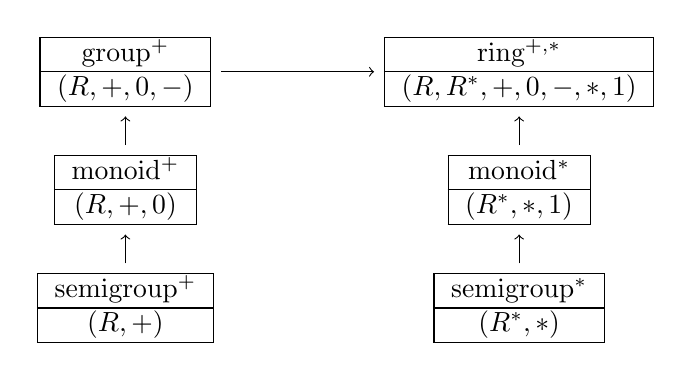
\begin{tikzpicture}
\node (sg) at (1,1)
    {\begin{tabular}{|c|}\hline 
      semigroup$^+$\\\hline
      $(R,+)$\\\hline
    \end{tabular}};
\node (mon) at (1,2.5)
    {\begin{tabular}{|c|}\hline 
      monoid$^+$\\\hline
      $(R,+,0)$\\\hline
    \end{tabular}};
\node (grp) at (1,4)
    {\begin{tabular}{|c|}\hline 
      group$^+$\\\hline
      $(R,+,0,-)$\\\hline
    \end{tabular}};
\node (ring) at (6,4)
    {\begin{tabular}{|c|}\hline 
      ring$^{+,*}$\\\hline
      $(R,R^*,+,0,-,*,1)$\\\hline
    \end{tabular}};
\node (sg1) at (6,1)
    {\begin{tabular}{|c|}\hline 
      semigroup$^*$\\\hline
      $(R^*,*)$\\\hline
    \end{tabular}};
\node (mon1) at (6,2.5)
    {\begin{tabular}{|c|}\hline 
      monoid$^*$\\\hline
      $(R^*,*,1)$\\\hline
    \end{tabular}};

\draw[->](sg)   -- (mon);
\draw[->](sg1)  -- (mon1); 
\draw[->](mon)  -- (grp); 
\draw[->](mon1) -- (ring); 
\draw[->](grp)  -- (ring); 
\end{tikzpicture}}
\end{myfig}
  
This problem\footnote{which seems negligible in this simple example, but in real life,
  each instance of multiple inheritance leads to a \emph{multiplication} of all
  dependent theories, which becomes an exponentially redundant management nightmare.} can
be alleviated by allowing theory inheritance via translations.  Instead of literally
inheriting the symbols and axioms from the source theory, we involve a symbol mapping
function (we call this a \defin{morphism}) in the process. This function maps source
formulae (i.e. built up exclusively from symbols visible in the source theory) into
formulae in the target theory by translating the source symbols.
  
\myfigref{rings-math} shows a theory graph that defines a theory of rings by importing
the monoid axioms via the morphism $\sigma$. With this translation, we do not have to
duplicate the \snippet{monoid} and \snippet{semigroup} theories and can even move the
definition of $\cdot^*$ operator into the theory of monoids, where it intuitively
belongs\footnote{On any monoid $M=(S,\circ,e)$, we have the $\cdot^*$ operator, which
  converts a set $S\subseteq M$ in to $S^*\deq\setst{r\in S}{r\ne e}$}.

\begin{myfig}{rings-math}{A Theory of Rings via Morphisms}
\fbox{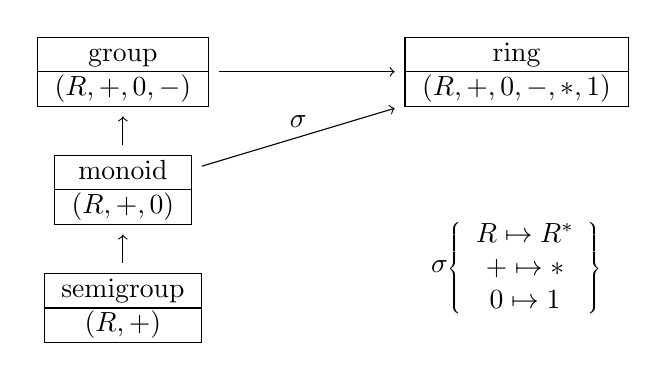
\begin{tikzpicture}
\node (sg) at (1,1)
    {\begin{tabular}{|c|}\hline 
      semigroup\\\hline
      $(R,+)$\\\hline
    \end{tabular}};
\node (mon) at (1,2.5)
    {\begin{tabular}{|c|}\hline 
      monoid\\\hline
      $(R,+,0)$\\\hline
    \end{tabular}};
\node (grp) at (1,4)
    {\begin{tabular}{|c|}\hline 
      group\\\hline
      $(R,+,0,-)$\\\hline
    \end{tabular}};

\node (ring) at (6,4)
    {\begin{tabular}{|c|}\hline 
      ring\\\hline
      $(R,+,0,-,*,1)$\\\hline
    \end{tabular}};
\node (sig) at (6,1.5)
   {$\sigma\deq\scriptscriptstyle\left\{\begin{array}{c}
      R\mapsto R^*\\+\mapsto *\\0\mapsto 1
    \end{array}\right\}$};

\draw[->](sg) -- (mon);
\draw[->](mon) -- (grp);
\draw[->](mon) -- node[above] {$\sigma$} (ring);
\draw[->](grp) -- (ring);
\end{tikzpicture}}
\end{myfig}

Formally, we extend the notion of inheritance given in \mysecref{theories} by
allowing a \twintoo{target}{theory} to import another a \twintoo{source}{theory}
\defin{via a morphism}: Let $\cS$ be a theory with theory-constitutive
elements\footnote{which may in turn be inherited from other theories} $t_1,\ldots,t_n$ and
$\sigma\colon\cS\to\cT$ a morphism, if we declare that $\cT$ imports $\cS$ via $\sigma$,
then $\cT$ {\defin{inherit}s} the theory-constitutive statements $\sigma(t_i)$ from
$\cS$. For instance, the theory of rings inherits the \indextoo{axiom}
$\allcdot{x}{x+0=x}$ from the theory of monoids as
$\sigma(\allcdot{x}{x+0=x})=\allcdot{x}{x*1=x}$.

To specify the formula mapping function, module \CTHmodule{spec} extends the
\element{imports} element by allowing it to have a child element \eldef{morphism},
which specifies a formula mapping by a set of recursive equations using the
\element{requation} element described in \mysecref{definitions}. The optional
attribute \attribute{type}{morphism} allows to specify whether the function is really
recursive (value \attval{recursive}{type}{morphism}) or pattern-defined (value
\attval{pattern}{type}{morphism}). As in the case of the \element{definition} element,
termination of the defined function can be specified using the optional child elements
\element{measure} and \element{ordering}, or the optional attributes
\attribute{uniqueness}{morphism} and \attribute{existence}{morphism}, which point to
uniqueness and existence assertions. Consistency\index{consistency} and
\indextoo{exhaustivity} of the recursive equations are specified by the optional
attributes \attribute{consistency}{morphism} and \attribute{exhaustivity}{morphism}.

\Mylstref{rings} gives the \omdoc representation of the theory graph in
\myfigref{rings-math}, assuming the theories in \mylstref{def-group}.

\begin{lstlisting}[label=lst:rings,
  caption={A Theory of Rings by Inheritance Via Renaming},
  index={derive,method,premise}]
<theory xml:id="ring"> 
  <symbol name="times"/><symbol name="one"/> 
  <structure name="add" from="?group"/>
  <structure name="mult" from="?monoid">
    <morphism> 
      <requation> 
        <OMOBJ><OMS cd="monoid" name="set"/></OMOBJ>
        <OMOBJ>
          <OMA><OMS cd="monoid" name="setstar"/>
            <OMS cd="semigroup" name="set"/>
          </OMA>
        </OMOBJ>
      </requation> 
      <requation> 
        <OMOBJ><OMS cd="monoid" name="op"/></OMOBJ>
        <OMOBJ><OMS cd="ring" name="times"/></OMOBJ>
      </requation> 
      <requation>
        <OMOBJ><OMS cd="monoid" name="neut"/></OMOBJ>
        <OMOBJ><OMS cd="ring" name="one"/></OMOBJ>
      </requation> 
    </morphism> 
  </imports> 
  <axiom xml:id="ring.distribution"> 
    <CMP><xthml:p><OMOBJ><OMS cd="semigroup" name="op"/></OMOBJ> distributes over 
      <OMOBJ><OMS cd="ring" name="times"/></OMOBJ> </xhtml:p>
    </CMP> 
  </axiom>
</theory>
\end{lstlisting}

To conserve space and avoid redundancy, \omdoc morphisms need only specify the values of
symbols that are translated; all other symbols are inherited literally.  Thus the set of
symbols inherited by an \element{imports} element consists of the symbols of the source
theory that are not in the domain of the morphism. In our example, the symbols $R$, $+$,
$0$, $-$, $*$, $1$ are visible in the theory of rings (and any other symbols the theory of
semigroups may have inherited). Note that we do not have a name clash from multiple
inheritance.
  
Finally, it is possible to hide symbols from the source theory by specifying them in the
\attribute{hiding}{morphism} attribute. The intended meaning is that the underlying
signature mapping is defined (total) on all symbols in the source theory except on the
hidden ones. This allows to define symbols that are local to a given theory, which helps
achieve data protection. Unfortunately, there is no simple interpretation of hiding in the
general case in terms of formula translations, see~\cite{CoFI:2004:CASL-RM,MAH-06-a} for
details. The definition of hiding used there is more general. The variant used here arises
as the special case where the hiding morphism, which goes against the import direction, is
an inclusion; then the symbols that are not in the image are the hidden ones.  If we
restrict ourselves to hiding defined symbols, then the situation becomes simpler to
understand: A morphism that hides a (defined) symbol $s$ will translate the
theory-constitutive elements of the source theory by expanding definitions. Thus $s$ will
not be present in the target theory, but all the contributions of the theory-constitutive
elements of the source theory will have been inherited. Say, we want to define the concept
of a sorting function, i.e. a function that --- given a list $L$ as input --- returns a
returns a permutation $L'$ of $L$ that is ordered. In the situation depicted in
\myfigref{rest:actualization}, we would the concept of an ordering function (a function
that returns a permutation of the input list that is ordered) with the help of predicates
\snippet{perm} and \snippet{ordered}. Since these are only of interest in the context
of the definition of the latter, they would typically be hidden in order to refrain from
polluting the name space.

As morphisms often contain common prefixes, the \element{morphism} element has an optional
\attribute{base}{morphism} attribute, which points to a chain of
morphisms\twin{morphism}{base}, whose \indextoo{composition} is taken to be the base of
this morphism. The intended meaning is that the new morphism coincides as a function with
the base morphism, wherever the specified pattern do not match, otherwise their
corresponding values take precedence over those in the \twintoo{base}{morphism}.
Concretely, the \attribute{base}{morphism} contains a whitespace-separated list of
\twintoo{URI}{reference}s to \element{structure} elements. Note that the order of the
references matters: they are ordered in order of the path in the local chain, i.e if we
have \snippet{base="\#\llquote{ref1}\ldots \#\llquote{refn}"} there must be theory
inclusions $\sigma_i$ with \snippet{xml:id="}\llquote{refi}\snippet{"}, such that the
target theory of $\sigma_{i-1}$ is the source theory of $\sigma_i$, and such that the
source theory of $\sigma_1$ and the target theory of $\sigma_n$ are the same as those of
the current view.

Finally, the \CTHmodule{spec} module adds two the optional attributes
\attribute{conservativity}{imports} and \attribute{conservativity-just}{imports} to
the \element{imports} element for stating and justifying \indextoo{conservativity}
(see the discussion below).
\end{tsection}

\begin{tsection}[id=views]{Views}
  
  We have seen that inheritance via morphisms provides a powerful mechanism for
  structuring and re-using theories and contexts. It turns out that the distinguishing
  feature of theory morphisms is that all theory-constitutive elements of the source
  theory are valid in the target theory (possibly after translation). This can be
  generalized to obtain even more structuring relations and thus possibilities for reuse
  among theories. Before we go into the \omdoc infrastructure, we will briefly introduce
  the mathematical model (see e.g.~\cite{Hutter:mocsv00} for details).

  A \defin{view} from a \twindef{source}{theory} $\cS$ to a \twindef{target}{theory} $\cT$
  is a mapping $\sigma$ from $\cS$ objects\footnote{Mathematical objects that can be
    represented using the only symbols of the source theory $\cS$.} to those of $\cT$,
  such that for every theory-constitutive statement $\bS$ of $\cS$, $\sigma(\bS)$ is
  provable in $\cT$ (we say that $\sigma(\bS)$ is a \defin{$\cT$-theorem}\index{theorem}).
   
  In \omdoc, we weaken this logical property to a structural one: We say that a
  theory-constitutive statement $\bS$ in theory $\cS$ is
  \twindef{structurally}{included} in theory $\cT$ via $\sigma$, if there is an
  assertional statement\twin{assertional}{element} $\bT$ in $\cT$, such that the content
  of $\bT$ is $\sigma(\bS)$.  Note that strictly speaking, $\sigma$ is only defined on
  formulae, so that if a statement $\bS$ is only given by a \element{CMP}, $\sigma(\bS)$
  is not defined. In such cases, we assume $\sigma(\bS)$ to contain a \element{CMP}
  element containing suitably translated mathematical vernacular. In this view, a
  \atwindef{structural}{theory}{inclusion} from $\cS$ to $\cT$ is a morphism
  $\sigma\colon\cS\to\cT$, such that every theory-constitutive element is structurally
  included in $\cT$.
  
  Note that an \element{imports} element in a theory $\cT$ with source theory $\cS$ as
  discussed in \mysecref{morphisms} induces a theory inclusion from $\cS$ into
  $\cT$\footnote{Note that in contrast to the inheritance relation induced by the
    \element{imports} elements the relation induced by general theory inclusions may be
    cyclic. A cycle just means that the theories participating in it are semantically
    equivalent.} (the theory-constitutive statements of $\cS$ are accessible in $\cT$
  after translation and are therefore structurally included trivially).  We call this kind
  of theory inclusion \defin{definitional}\atwin{definitional}{theory}{inclusion}, since
  it is a theory inclusion by virtue of the definition of the target theory.  For all
  other theory inclusions (we call them {\atwindef{postulated}{theory}{inclusion}s}), we
  have to establish the theory inclusion property by proving the translations of the
  theory-constitutive statements of the source theory (we call these translated formulae
  \twindef{proof}{obligation}).

  The benefit of a theory inclusion is that all {\indextoo{theorem}s},
  \indextoo{proof}s, and \twintoo{proof}{method}s of the source theory can be used
  (after translation) in the target theory (see \mysecref{induced-assertions}).
  Obviously, the transfer approach only depends on the theorem inclusion property, and we
  can extend its utility by augmenting the theory graph by more theory morphisms than just
  the definitional ones (see~\cite{FaGu93} for a description of the {\imps} theorem
  proving system that makes heavy use of this idea).  We use the infrastructure presented
  in this chapter to structure a collection of theories as a \indextoo{graph} --- the
  \twindef{theory}{graph} --- where the nodes are theories and the links are theory
  inclusions (definitional and postulated ones).

  We call a theory inclusion $\sigma\colon\cS\to\cT$ \defin{conservative}, iff $\bA$ is
  already a $\cS$-theorem for all $\cT$-theorems of the from $\sigma(\bA)$. If the
  morphism $\sigma$ is the identity, then this means the local axioms in $\cT$ only affect
  the local symbols of $\cT$, and do not the part inherited from $\cS$. In particular,
  conservative extensions of consistent theories cannot be inconsistent. For instance, if
  all the local theory-constitutive elements in $\cT$ are symbol declarations with
  definitions, then conservativity is guaranteed by the special form of the
  definitions. We can specify conservativity of a theory inclusion via the
  \attributeshort{conservativity} attribute. The values
  \attvalshort{conservative}{conservativity} and
  \attvalshort{definitional}{conservativity} are used for the two cases discussed
  above. There is a third value: \attvalshort{monomorphism}{conservativity}, which we
  will not explain here, but refer the reader to~\cite{MAH-06-a}.

  \omdoc implements the concept of view in the \indextoo{top-level} \eldef{view}
  element. It has the required attributes \attribute{from}{view} and \attribute{to}{view},
  which point to the source- and target theories and contains a \element{morphism} child
  element as described above to define the translation function. A subsequent (possibly
  empty) set of \element{obligation} elements can be used to mark up proof obligations for
  the theory-constitutive elements of the source theory.

  An \eldef{obligation} is an empty element whose \attribute{assertion}{obligation}
  attribute points to an \element{assertion} element that states that the
  theory-constitutive statement specified by the \attribute{induced-by}{obligation}
  (translated by the morphism in the parent \element{view}) is provable in the target
  theory. Note that a \element{view} element must contain \element{obligation}
  elements for all theory-constitutive elements (inherited or local) of the source theory
  to be correct.

\mylstref{view} shows a theory inclusion from the theory
\snippet{group} defined in \mylstref{def-group} to itself. The morphism just
maps each element of the base set to its inverse. A good application for this kind
of theory morphism is to import claims for symmetric (e.g. with respect to the
function \snippet{inv}, which serves as an involution in \snippet{group})
cases via this theory morphism to avoid explicitly having to prove them (see
\mysecref{induced-assertions}).

\begin{lstlisting}[label=lst:view,mathescape,
  caption={A Theory Inclusion for Groups},
  index={view,morphism,requation,assertion}]
<assertion xml:id="conv.assoc">$\allcdot{x,y,z\in{M}}{z\circ(y\circ x)=(z\circ y)\circ x}$</assertion>
<assertion xml:id="conv.closed" theory="semigroup">$\allcdot{x,y\in{M}}{y\circ x\in{M}}$</assertion>
<assertion xml:id="left.unit" theory="monoid">$\allcdot{x\in{M}}{e\circ x= x}$</assertion>
<assertion xml:id="conv.inv" theory="group">$\allcdot{x,y\in{M}}{x\circ x^{-1}=e}$</assertion>
<view xml:id="grp-conv-grp" from="#group" to="#group">
  <morphism><requation>$X\circ Y\leadsto Y\circ X$</requation></morphism>
  <obligation assertion="#conv.closed" induced-by="#closed.ax"/>
  <obligation assertion="#conv.assoc" induced-by="#assoc.ax"/>
  <obligation assertion="#left.unit" induced-by="#unit.ax"/>
  <obligation assertion="#conv.inv" induced-by="#inv.ax"/>
</view>  
\end{lstlisting}
\end{tsection}

\begin{tsection}[id=restricting-inference,short=Local/Required Theory Inclusions]{Local- and Required Theory Inclusions}
  In some situations, we need to pose well-definedness conditions on theories,
  e.g. that a specification of a program follows a certain security model, or that
  a parameter theory used for actualization satisfies the assumptions made in the
  formal parameter theory; (see \mychapref{natlist} for a discussion). If these
  conditions are not met, the theory intuitively does not make sense. So rather
  than simply stating (or importing) these assumptions as theory-constitutive
  statements --- which would make the theory inconsistent, when they are not met
  --- they can be stated as well-definedness conditions. Usually, these conditions
  can be posited as theory inclusions, so checking these conditions is a purely
  structural matter, and comes into the realm of \omdoc's structural methods.

  \omdoc provides the empty \eldef{inclusion} element for this purpose. It can
  occur anywhere as a child of a \element{theory} element and its
  \attribute{via}{inclusion} attribute points to a theory inclusion, which is
  required to hold in order for the parent theory to be well-defined.
  
  If we consider for instance the situation in
  \myfigref{rest:actualization}\footnote{This example is covered in detail in
    \mychapref{natlist}.}.  There we have a theory \snippet{OrdList} of lists that is
  generic in the elements (which is assumed to be a totally ordered set, since we want to
  talk about ordered lists). We want to to instantiate \snippet{OrdList} by applying it
  to the theory \snippet{NatOrd} of natural numbers and obtain a theory
  \snippet{NatOrdList} of lists of natural numbers by importing the theory
  \snippet{OrdList} in \snippet{NatOrdList}. This only makes sense, if
  \snippet{NatOrd} is a totally ordered set, so we add an \element{inclusion} element
  in the statement of theory \snippet{NatOrdList} that points to a theory inclusion of
  \snippet{TOSet} into \snippet{OrdNat}, which forces us to verify the axioms of
  \snippet{TOSet} in \snippet{OrdNat}.

\begin{myfig}{rest:actualization}{A Structured Specification of Lists (of
    Natural Numbers)}
  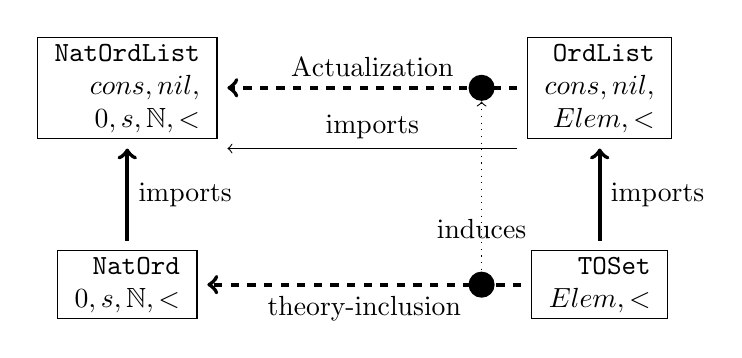
\begin{tikzpicture}  \node (natordlist) at (0,2.5) 
    {\begin{tabular}{|r|}\hline 
      {\tt{NatOrdList}}\\
      $cons, nil,$\\
      $0,s,{\mathbb{N}},<$\\\hline
    \end{tabular}};
  \node (natord) at (0,0) 
    {\begin{tabular}{|r|}\hline 
      {\tt{NatOrd}}\\
      $0,s,{\mathbb{N}},<$\\\hline
    \end{tabular}};
  \node (toset) at (6,0) 
    {\begin{tabular}{|r|}\hline 
      {\tt{TOSet}}\\
      $Elem,<$\\\hline
    \end{tabular}};
  \node (ordlist) at (6,2.5) 
    {\begin{tabular}{|r|}\hline 
      {\tt{OrdList}}\\
      $cons, nil,$\\
      $Elem,<$\\\hline
    \end{tabular}};
  \node[circle,fill] (act1) at (4.5,2.5) {};
  \node[circle,fill] (act2) at (4.5,0) {};
  \draw [->,line width=1.5pt] (natord) -- node[right]{imports} (natordlist);
  \draw [->,line width=1.5pt] (toset) -- node[right]{imports} (ordlist);
  \draw [->,dashed,line width=1.5pt] (toset) -- node[below]{theory-inclusion} (natord);
  \draw [->,dashed,line width=1.5pt] (ordlist) -- node[above]{Actualization} (natordlist);
  \draw [->] (ordlist.south west) -- node[above]{imports} (natordlist.south east);
  \draw [<-,dotted,near end] (act1) -- node{induces} (act2);
\end{tikzpicture}\quad
  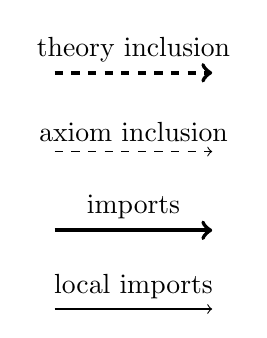
\begin{tikzpicture}
    \draw[->,dashed,line width=1.5pt] (0,3) -- node[above]{theory inclusion} (2,3);
    \draw[->,dashed] (0,2) -- node[above]{axiom inclusion} (2,2);
    \draw[->,line width=1.5pt] (0,1) -- node[above]{imports} (2,1);
    \draw[->] (0,0) -- node[above]{local imports} (2,0);
 \end{tikzpicture}
\end{myfig}

Furthermore note, that the inclusion of \snippet{OrdList} into \snippet{NatOrdList}
should not include the \snippet{TOSet} axioms on orderings, since this would defeat the
purpose of making them a precondition to well-definedness of the theory
\snippet{NatOrdList}. Therefore \omdoc follows the ``development graph model'' put
forward in~\cite{Hutter:mocsv00} and generalizes the notion of theory inclusions even
further: A formula mapping between theories $\cS$ and $\cT$ is called a
\atwindef{local}{theory}{inclusion} or \twindef{axiom}{inclusion}, if the theory
inclusion property holds for the local theory-constitutive statements of the source
theory.  To distinguish this from the notion of a proper \twintoo{theory}{inclusion} ---
where the theory inclusion property holds for all theory constitutive statements of $\cS$
(even the inherited ones) --- we call the latter one \defin{global}. Of course all
global theory inclusions are also local ones, so that the new notion is a true
generalization. Note that the structural inclusions of an \twintoo{axiom}{inclusion} are
not enough to justify translated source theorems in the target theory.

To allow for a local variant of inheritance, the \CTHmodule{spec} module adds an
attribute \attribute{type}{imports} to the \element{imports} element. This can take
the values \attval{global}{type}{imports} (the default) and
\attval{local}{type}{imports}. In the latter case, only the theory-constitutive
statements that are local to the source theory are imported.
  
Furthermore, the \CTHmodule{spec} module introduces the \eldef{axiom-inclusion}
element for \atwintoo{local}{theory}{inclusion}s. This has the same attributes as
\element{view}: \attribute{from}{axiom-inclusion} to specify source
theory, \attribute{to}{axiom-inclusion} for the target theory. It also allows
\element{obligation} elements as children.
\end{tsection}

\begin{tsection}[id=induced-assertions,short=Induced Assertions]{Induced Assertions and Expositions}
  The main motivation of theory inclusions is to be able to transport mathematical
  statements from the \twintoo{source}{theory} to the \twintoo{target}{theory}. In
  \omdoc, this operation can be made explicit by the attributes
  \attributeshort{generated-from} and \attributeshort{generated-via} that the module
  \CTHmodule{spec} adds to all \twintoo{mathematical}{statement}s.  On a statement
  $\bT$, the second attribute points to a \twintoo{theory}{inclusion} $\sigma$ whose
  target is (imported into the) current theory, the first attribute points to a statement
  $\bS$ in that theory which is of the same type (i.e. has the same \omdoc element name)
  as $\bT$.  The content of $\bT$ must be (equivalent to) the content of $\bS$ translated
  by the morphism of $\sigma$.
  
  In the context of the theory inclusion in \mylstref{view}, we
  might have the following situation:
\begin{lstlisting}[label=lst:assertion-translation,mathescape,
  caption={Translating a Statement via a Theory Inclusion},
  index={translated-from,translated-via}]
<assertion xml:id="foo" type="theorem">$\ldots$</assertion>
<proof xml:id="foo.pf" for="#foo">$\ldots$</proof>
<assertion xml:id="target" induced-by="#foo" induced-via="#grp-conv-grp"> 
  $\ldots$
</assertion>
\end{lstlisting}
Here, the second assertion is induced by the first one via the theory inclusion in
\mylstref{view}, the statement of the theorem is about the inverses.  In
particular, the proof of the second theorem comes for free, since it can also be induced
from the proof of the first one.

In particular we see that in \omdoc documents, not all statements are automatically
generated by translation e.g. the proof of the second assertion is not explicitly stated.
Mathematical knowledge management systems like knowledge bases might choose to do so, but
at the document level we do not mandate this, as it would lead to an explosion of the
document sizes. Of course we could cache the transformed proof giving it the same ``cache
attribute state''.

Note that not only statements like assertions and proofs can be translated via theory
inclusions, but also whole documents: Say that we have course materials for elementary
algebra introducing monoids and groups via \twintoo{left}{unit}s and
\twintoo{left}{inverse}s, but want to use examples and exercises from a book that
introduces them using \twintoo{right}{unit}s and \twintoo{right}{inverse}s. Assuming
that both are formalized in \omdoc, we can just establish a theory morphism much like
the one in \mylstref{view}. Then we can automatically translate the
exercises and examples via this theory inclusion to our own setting by just applying the
morphism to all formulae in the text\footnote{There may be problems, if mathematical
  statements are verbalized; this can currently not be translated directly, since it would
  involve language processing tools much beyond the content processing tools described in
  this {\report}. For the moment, we assume that the materials are written in a controlled
  subset of mathematical vernacular that avoids these problems.}  and obtain exercises and
examples that mesh well with our introduction. Of course there is also a theory inclusion
in the other direction, which is an inverse, so our colleague can reuse our course
materials in his right-leaning setting.

Another example is the presence of different normalization factors in physics or branch
cuts in elementary complex functions. In both cases there is a plethora of definitions,
which all describe essentially the same objects (see e.g.~\cite{BraCor:raefca02} for an
overview over the branch cut situation). Reading materials that are based on the ``wrong''
definition is a nuisance at best, and can lead to serious errors. Being able to adapt
documents by translating them from the author theory to the user theory by a previously
established theory morphism can alleviate both.

Mathematics and science are full of such situations, where objects can be viewed from
different angles or in different representations. Moreover, no single representation is
``better'' than the other, since different views reveal or highlight different aspects of
the object (see~\cite{KohKoh:esmk05} for a systematic account). Theory inclusions seem
uniquely suited to formalize the structure of different views in mathematics and their
interplay, and the structural markup for theories in \omdoc seems an ideal platform for
offering added-value services that feed on these structures without committing to a
particular formalization or foundation of mathematics.
\end{tsection}

\end{tchapter}
%%% Local Variables: 
%%% mode: latex
%%% TeX-master: "omdoc"
%%% End: 

% LocalWords:  cpx def requation lst setstar cd mathescape ti thi cic bic aic
% LocalWords:  aia im axa xunit linewidth arcangle ai ima imb axb axc param ord
% LocalWords:  elem toset nat elt nats incl morph natlist dec adt  sg dg truecm
% LocalWords:  mon grp mult tn  TOSet NatOrd sortdef TOset CMP FMP pspic TOSet
% LocalWords:  pt linestyle omdoc elal dgraph conv xref yunit ref ic tcic ns th
% LocalWords:  cpx def requation lst setstar cd mathescape ti thi cic bic aic
% LocalWords:  aia im axa xunit linewidth arcangle ai ima imb axb axc param ord
% LocalWords:  elem toset nat elt nats incl morph natlist dec adt  sg ref conv
% LocalWords:  mon grp mult tn  TOSet NatOrd sortdef TOset OrdList OrdNat TOSet
% LocalWords:  NatOrdList pf attr sig OMOBJ OMA globals refi inv TOSet TOSet
% LocalWords:  TOSet TOSet TOSet TOSet TOSet TOSet TOSet TOSet TOSet TOSet foo
% LocalWords:  Hutter mocsv00 conv.assoc assoc.ax BraCor raefca02 KohKoh esmk05

%%%%%%%%%%%%%%%%%%%%%%%%%%%%%%%%%%%%%%%%%%%%%%%%%%%%%%%%%%%%%%%%%%%%%%%%%
% This file is part of the LaTeX sources of the OMDoc 1.3 specification
% Copyright (c) 2006 Michael Kohlhase
% This work is licensed by the Creative Commons Share-Alike license
% see http://creativecommons.org/licenses/by-sa/2.5/ for details
%%%%%%%%%%%%%%%%%%%%%%%%%%%%%%%%%%%%%%%%%%%%%%%%%%%%%%%%%%%%%%%%%%%%%%%%%

\begin{tchapter}[id=pres,short=Notation and Presentation]{Notation and Presentation (Module {\PRESmodule{spec}})}
  The main difference of {\omdocv{1.3}} is that it uses the notation system developed
  in~\cite{cmueller:thesis:10,KMR:NoLMD08}. This system is already supported by the JOMDoc
  system~\cite{JOMDoc:on}.
\end{tchapter}
%%% Local Variables: 
%%% mode: latex
%%% TeX-master: "omdoc"
%%% End: 

% LocalWords:  xsl omstyle xref  xslt pmml cmml mathematica tex lang en PCDATA
% LocalWords:  lst linebreak OMSTR em br href om omlet cd quant comm qtpres gr
% LocalWords:  ter gemeinsamer Teiler sen ta tion ombind arith lbrack rbrack mi
% LocalWords:  crossref hyperref sty dvips mathml mfrac linethickness omclass
% LocalWords:  frac lt gt msup pres mroot var bvar ci OMATP msub mn eq attribs
% LocalWords:  csymbol definitionURL cn mathescape sem OMFOREIGN qtstylen crid
% LocalWords:  cr ns mrow xlink rt mo xmlns attr elt infixl infixr CDATA
% LocalWords:  recurse omdoc html CMP qtstyle OMBVAR forall OMV OMA OMOBJ gcd
% LocalWords:  ggT OMATTR Prolog OMI

%%%%%%%%%%%%%%%%%%%%%%%%%%%%%%%%%%%%%%%%%%%%%%%%%%%%%%%%%%%%%%%%%%%%%%%%%
% This file is part of the LaTeX sources of the OMDoc 1.3 specification
% Copyright (c) 2016 Michael Kohlhase.
% Source at https://github.com/KWARC/OMDoc/tree/master/doc/spec
% This work is licensed by the Creative Commons Share-Alike license
% see http://creativecommons.org/licenses/by-sa/2.5/ for details
%%%%%%%%%%%%%%%%%%%%%%%%%%%%%%%%%%%%%%%%%%%%%%%%%%%%%%%%%%%%%%%%%%%%%%%%%

\begin{tchapter}[id=ext,short=Auxiliary Elements]{Auxiliary Elements (Module {\EXTmodule{spec}})}

  Up to now, we have been mainly concerned with providing elements for marking up the
  inherent structure of mathematical knowledge in mathematical statements and
  theories. Now, we interface {\omdoc} documents with the Internet in general and
  mathematical software systems in particular. We can thereby generate presentations from
  {\omdoc} documents where formulae, statements or even theories that are active
  components that can directly be manipulated by the user or mathematical software
  systems. We call these documents {\twindef{active}{document}s}.  For this we have to
  solve two problems: an abstract interface for calls to external (web)
  services\footnote{Compare {\mychapref{rpc}} in the {\omdoc} Primer.} and a way of
  storing application-specific data in {\omdoc} documents (e.g. as arguments to the system
  calls).

  The module {\EXTmodule{spec}} provides a basic infrastructure for these tasks in
  {\omdoc}. The main purpose of this module is to serve as an initial point of entry. We
  envision that over time, more sophisticated replacements will be developed driven by
  applications.

\begin{myfig}{qtcode}{The {\omdoc} Auxiliary Elements for Non-{\xml} Data}
\begin{scriptsize}
\begin{tabular}{|>{\tt}l|>{\tt}l|>{\tt}p{4.5truecm}|c|>{\tt}p{3truecm}|}\hline
{\rm Element}& \multicolumn{2}{l|}{Attributes\hspace*{2.25cm}} & D & Content  \\\hline
             & {\rm Req.} & {\rm Optional}     & C &           \\\hline\hline
 private     &            & xml:id, for, theory, 
                               requires, type, reformulates, class, style
                                               & +  & CMP*, data+ \\\hline
% theory is optional for code, isn't it?? --clange
 code        &            & xml:id, for, theory, 
                              requires, type, class, style
                              & +  & CMP*, input?, output?, effect?, data+ \\\hline
 input       &            & xml:id, style, class   & + & CMP*, FMP*\\\hline
 output      &            & xml:id, style, class   & + & CMP*, FMP*\\\hline
 effect      &            & xml:id, style, class   & + & CMP*, FMP*\\\hline
 data        &            & format, href, size, original, pto, pto-version 
                                               & -- & <![CDATA[\ldots]]> \\\hline
\end{tabular}
\end{scriptsize}
\end{myfig}


\begin{tsection}[id=private]{Non-XML Data and Program Code in OMDoc}
  
  The representational infrastructure for mathematical knowledge provided by {\omdoc} is
  sufficient as an output- and library format for
  {\atwintoo{mathematical}{software}{system}s} like {\twintoo{computer algebra}{system}s},
  {\twintoo{theorem}{prover}s}, or {\atwintoo{theory}{development}{system}s}. In
  particular, having a standardized output- and library format like {\omdoc} will enhance
  system interoperability, and allows to build and deploy general storage and library
  management systems (see {\mysecref{mbase}} for an {\omdoc} example). In fact this was
  one of the original motivations for developing the format.
  
  However, most mathematical software systems need to store and communicate
  system-specific data that cannot be standardized in a general knowledge-representation
  format like {\omdoc}. Examples of this are pieces of {\indextoo{program}} code, like
  tactics or proof search heuristics of tactical theorem provers or linguistic data of
  {\atwintoo{proof}{presentation}{system}s}.  Only if these data can be integrated into
  {\omdoc}, it will become a full storage and communication format for mathematical
  software systems. One characteristic of such system-specific data is that it is often
  not in {\xml} syntax, or its format is not fixed enough to warrant for a general {\xml}
  encoding.
  
  For this kind of data, {\omdoc} provides the {\eldef{private}} and {\eldef{code}}
  elements. As the name suggests, the latter is intended for program code\footnote{There
    is a more elaborate proposal for treating program code in the {\omdoc} arena
    at~\cite{Kohlhase:codemlspec}, which may be integrated into {\omdoc} as a separate
    module in the future, for the moment we stick to the basic approach.} and the former
  for system-specific data that is not program code.
  
  The attributes of these elements are almost identical and contain metadata
  information identifying system requirements and relations to other {\omdoc}
  elements. We will first describe the shared attributes and then describe the
  elements themselves.
\begin{description}
\item[{\attribute[ns-attr=xml]{id}{private, code}}] for identification.
\item[{\attribute{theory}{private, code}}] specifies the mathematical theory (see
  {\mysecref{theories}}) that the data is associated with.
\item[{\attribute{for}{private, code}}] allows to attach data to some other {\omdoc}
  element. Attaching {\element{private}} elements to {\omdoc} elements is the main
  mechanism for system-specific extension of {\omdoc}.
\item[{\attribute{requires}{private, code}}] specifies other data this element depends
  upon as a whitespace-separated list of {\twintoo{URI}{reference}s}.  This allows to
  factor private data into smaller parts, allowing more flexible data storage and
  retrieval which is useful for program code or private data that relies on program
  code. Such data can be broken up into procedures and the call-hierarchy can be encoded
  in {\attribute{requires}{private, code}} attributes. With this information, a storage
  application based on {\omdoc} can always communicate a minimal complete code set to the
  requesting application.
\item[{\attribute{reformulates}{private}}] ({\element{private}} only) specifies a set of
  {\omdoc} elements whose knowledge content is reformulated by the {\element{private}}
  element as a whitespace-separated list of {\twintoo{URI}{reference}s}. For instance, the
  knowledge in the assertion in {\mylstref{private-simplify}} can be used as an algebraic
  simplification rule in the {\scsys{Analytica}}
  {\twintoo{theorem}{prover}}~\cite{ClaKoh:sda03} based on the {\scsys{Mathematica}}
  {\twintoo{computer algebra}{system}}.
\end{description}

The {\element{private}} and {\element{code}} elements contain an optional
{\element{metadata}} element and a set of {\element{data}} elements that contain
or reference the actual data.

\begin{lstlisting}[label=lst:private-simplify,mathescape,
  caption={Reformulating Mathematical Knowledge},index={private,data}]
  <assertion xml:id="ALGX0">
    <CMP><xhtml:p>If $a,b,c,d$ are numbers, then we have $a+b(c+d)=a+bc+bd$.</xhtml:p></CMP>
  </assertion>
  <private xml:id="alg-expr-1" pto="Analytica" reformulates="ALGX0">
   <data format="mathematica-5.0">
     <![CDATA[SIMPLIFYRULES[a_ + b_*(c_ + d_) :> a + b*c + b*d /; NumberQ[b]]]]>
   </data>
  </private>
\end{lstlisting}

The {\eldef{data}} element contains the data in a {\snippetin{CDATA}} section.  Its
{\attribute{pto}{data}} attribute contains a whitespace-separated list of
{\twintoo{URI}{reference}s} which specifies the set of systems to which the data are
related.  The intention of this field is that the data is visible to all systems, but
should only manipulated by a system that is mentioned here. The
{\attribute{pto-version}{data}} attribute contains a whitespace-separated list of version
number strings; this only makes sense, if the value of the corresponding
{\attribute{pto}{data}} is a singleton. Specifying this may be necessary, if the data or
even their format change with versions.

If the content of the {\element{data}} element is too large to store directly in the
{\omdoc} or changes often, then the {\element{data}} element can be augmented by a link,
specified by a {\twintoo{URI}{reference}} in the {\attribute{href}{data}} attribute. If
the {\element{data}} element is non-empty and there is a
{\attribute{href}{data}}\footnote{e.g. if the {\element{data}} content serves as a cache
  for the data at the URI, or the {\element{data}} content fixes a snapshot of the
  resource at the URI}, then the optional attribute {\attribute{original}{data}} specifies
whether the {\element{data}} content (value {\attval{local}{original}{data}}) or the
external resource (value {\attval{external}{original}{data}}) is the original. The
optional {\attribute{size}{data}} attribute can be used to specify the content size (if
known) or the resource identified in the {\attribute{href}{data}} attribute. The
{\element{data}} element has the (optional) attribute {\attribute{format}{data}} to
specify the format the data are in, e.g.  {\attval{image/jpeg}{format}{data}} or
{\attval{image/gif}{format}{data}} for image data, {\attval{text/plain}{format}{data}} for
text data, {\attval{binary}{format}{data}} for system-specific binary data, etc. It is
good practice to use the {\twintoo{MIME}{type}s}~\cite{FreBor:MIME96} for this purpose
whenever applicable.  Note that in a {\element{private}} or {\element{code}} element, the
{\element{data}} elements must differ in their {\attribute{format}{data}} attribute. Their
order carries no meaning.

In {\mylstref{private-fig}} we use a {\element{private}} element to specify data
for an image\footnote{actually {\myfigref{bourbaki}} from {\mychapref{algebra}}}
in various formats, which is useful in a content markup format like {\omdoc} as
the transformation process can then choose the most suitable one for the target.

\begin{lstlisting}[label=lst:private-fig,index={private,data},
  caption={A {\element{private}} Element for an Image}]
<private xml:id="legacy">
  <metadata>
    <dc:title>A fragment of Bourbaki's Algebra</dc:title>
    <dc:creator role="trl">Michael Kohlhase</dc:creator> 
    <dc:date action="created">2002-01-03T0703</dc:date>
    <dc:description>A fragment of Bourbaki's Algebra</dc:description>
    <dc:source>Nicolas Bourbaki, Algebra, Springer Verlag 1974</dc:source>
    <dc:type>Text</dc:type>
  </metadata>
  <data format="application/x-latex" href="legacy.tex"/>
  <data format="image/jpg" href="legacy.jpeg"/>
  <data format="application/postscript" href="legacy.ps"/>
  <data format="application/pdf" href="legacy.pdf"/>
</private>
\end{lstlisting}

The {\element{code}} element is used for embedding pieces of program code into an {\omdoc}
document.  It contains the documentation elements {\eldef{input}}, {\eldef{output}}, and
{\eldef{effect}} that specify the behavior of the procedure defined by the code fragment.
The {\element{input}} element describes the structure and scope of the input arguments,
{\element{output}} the outputs produced by calling this code on these elements, and
{\element{effect}} any side effects the procedure may have.  They contain a
{\twintoo{multilingual}{group}} of {\element{CMP}} elements with an optional
{\element{FMP}} group for a formal description. The latter may be used for program
verification purposes. If any of these elements are missing it means that we may not make
any assumptions about them, not that there are no inputs, outputs or effects. For
instance, to specify that a procedure has no side-effects we need to specify something
like 
\begin{lstlisting}
<effect><CMP><xhtml:p>None.</xhtml:p></CMP></effect>
\end{lstlisting}

These documentation elements are followed by a set of {\element{data}} elements
that contain or reference the program code itself. {\Mylstref{omlet1}} shows an
example of a {\element{code}} element used to store {\indextoo{Java}} code for an
applet.

\begin{lstlisting}[label=lst:callMint,mathescape,escapechar=\%,
  caption={The Program Code for a Java Applet},
  index={code,input,output,effect,data}]
<code xml:id="callMint" requires="org.riaca.cas"> 
  <metadata>
    <dc:description>
      The multiple integrator applet. It puts up a user interface, queries the user for a 
      function, which it then integrates by calling one of several computer algebra systems. 
    </dc:description>
  </metadata>
  <data format="application/x-java-applet">
    <![CDATA[$\ldots$ %\llquote{the {\snippet{callMint}} code goes here}% $\ldots$]]>
  </data> 
  <input><CMP><xhtml:p>None: the applet handles input itself.</xhtml:p></CMP></input> 
  <output><CMP><xhtml:p>The result of the integration.</xhtml:p></CMP></output>
  <effect><CMP><xhtml:p>None.</xhtml:p></CMP></effect> 
</code>
\end{lstlisting}
\end{tsection}

\begin{tsection}[id=applets]{Applets and External Objects in OMDoc}
  
  Web-based text markup formats like {\html} have the concept of an
  {\twintoo{external}{object}} or ``{\indextoo{applet}}'', i.e.  a program that can in
  some way be executed in the browser or web client during document manipulation. This is
  one of the primary format-independent ways used to enliven parts of the document.  Other
  ways are to change the {\twintoo{document}{object model}} via an embedded programming
  language (e.g.  {\indextoo{JavaScript}}). As this method ({\twintoo{dynamic}{HTML}}) is
  format-dependent\footnote{In particular, the JavaScript references the {\html} DOM,
    which in our model is created by a presentation engine on the fly.}, it seems
  difficult to support in a content markup format like {\omdoc}.
  
  The challenge here is to come up with a format-independent representation of the applet
  functionality, so that the {\omdoc} representation can be transformed into the specific
  form needed by the respective presentation format.  Most user agents for these
  presentation formats have built-in mechanisms for processing common data types such as
  text and various image types. In some instances the user agent may pass the processing
  to an external application (``{\indextoo{plug-in}s}'').  These need information about
  the location of the object data, the {\twintoo{MIME}{type}} associated with the object
  data, and additional values required for the appropriate processing of the object data
  by the object handler at run-time.

\begin{myfig}{qtomlet}{The {\omdoc} Elements for External Objects}
\begin{scriptsize}
\begin{tabular}{|>{\tt}l|>{\tt}l|>{\tt}p{4cm}|c|>{\tt}l|}\hline
{\rm Element}& \multicolumn{2}{l|}{Attributes} & D & Content  \\\hline
             & {\rm Req.} & {\rm Optional}     & C &           \\\hline\hline
 omlet       & data,  & xml:id, action, show, actuate, class, style & +  &
                    (\llquote{{\element{CMP}} content} | param)*,private*,code*\\
 param   & name & value, valuetype & - & EMPTY\\\hline
\end{tabular}
\end{scriptsize}
\end{myfig}

In {\omdoc}, we use the {\eldef{omlet}} element for applets. It generalizes the {\html}
{\indextoo{applet}} concept in two ways: The computational engine is not restricted to
{\indextoo{plug-in}s} of the browser (we do not know what the result format and
presentation engine will be) and the program code can be included in the {\omdoc}
document, making document-centered computation easier to manage.
  
  Like the {\element[ns-elt=xhtml]{object}} tag, the {\element{omlet}} element can be used
  to wrap any text. In the {\omdoc} context, this means that the children of the
  {\element{omlet}} element can be any elements or text that can occur in the
  {\element{CMP}} element together with {\element{param}} elements to specify the
  arguments. The main presentation intuition is that the applet reserves a rectangular
  space of a given pre-defined size (specified in the {\css} markup\twin{CSS}{markup} in
  the {\attribute{style}{omlet}} attribute; see {\mylstref{omlet1}}) in the result
  document presentation, and hands off the presentation and interaction with the document
  in this space to the applet process. The data for the external object is referenced in
  two possible ways. Either via the {\attribute{data}{omlet}} attribute, which contains a
  {\twintoo{URI}{reference}} that points to an {\omdoc} {\element{code}} or
  {\element{private}} element that is accessible (e.g. in the same {\omdoc}) or by
  embedding the respective {\element{code}} or {\element{private}} elements as children at
  the end of the {\element{omlet}} element. This indirection allows us to reuse the
  machinery for storing code in {\omdoc}s. For a simple example see {\mylstref{omlet1}}.
  
  The behavior of the external object is specified in the attributes
  {\attribute{action}{omlet}}, {\attribute{show}{omlet}} and {\attribute{actuate}{omlet}}
  attributes\footnote{These latter two attributes are modeled after the
    {\xlink}~\cite{DeRMal:xlink01} attributes {\attributeshort{show}} and
    {\attributeshort{actuate}}.}.
  
  The {\attribute{action}{omlet}} specified the intended action to be performed with the
  data. For most objects, this is clear from the {\twintoo{MIME}{type}}. Images are to be
  displayed, audio formats will be played, and application-specific formats are passed on
  to the appropriate {\indextoo{plug-in}}. However, for the latter (and in particular for
  program code), we might actually be interested to display the data in its raw (or
  suitably presented) form. The {\attribute{action}{omlet}} addresses this need, it has
  the possible values {\attval{execute}{action}{omlet}} (pass the data to the appropriate
  plug-in or execute the program code), {\attval{display}{action}{omlet}} (display it to
  the user in audio- or visual form), and {\attval{other}{action}{omlet}} (the action is
  left unspecified).
  
  The {\attribute{show}{omlet}} attribute is used to communicate the desired presentation
  of the ending resource on traversal from the starting resource. It has one of the values
  {\attval{new}{show}{omlet}} (display the object in a new document),
  {\attval{replace}{show}{omlet}} (replace the current document with the presentation of
  the external object), {\attval{embed}{show}{omlet}} (replace the {\element{omlet}}
  element with the presentation of the external object in the current document), and
  {\attval{other}{show}{omlet}} (the presentation is left unspecified).
  
  The {\attribute{actuate}{omlet}} attribute is used to communicate the desired timing of
  the action specified in the {\attribute{action}{omlet}} attribute.  Recall that {\omdoc}
  documents as content representations are not intended for direct viewing by the user,
  but appropriate presentation formats are derived from it by a ``presentation process''
  (which may or may not be incorporated into the user agent). Therefore the
  {\attribute{actuate}{omlet}} attribute can take the values
  {\attval{onPresent}{action}{omlet}} (when the presentation document is generated),
  {\attval{onLoad}{action}{omlet}} (when the user loads the presentation document),
  {\attval{onRequest}{action}{omlet}} (when the user requests it, e.g. by clicking in the
  presentation document), and {\attval{other}{action}{omlet}} (the timing is left
  unspecified).
  
  The simplest form of an {\element{omlet}} is just the embedding of an external object
  like an image as in {\mylstref{omlet-image}}, where the {\attribute{data}{omlet}}
  attribute points to the {\element{private}} element in {\mylstref{private-fig}}. For
  presentation, e.g. as {\xhtml} in a modern browser, this would be transformed into an
  {\element[ns-elt=xhtml]{object}} element~\cite{W3C:xhtml2000}, whose specific attributes
  are determined by the information in the {\element{omlet}} element here and those
  {\element{data}} children of the {\element{private}} element specified in the
  {\attribute{data}{omlet}} attribute of the {\element{omlet}} that are chosen for
  presentation in {\xhtml}. If the action specified in the {\attribute{action}{omlet}}
  attribute is impossible (e.g. if the contents of the {\attribute{data}{omlet}} target
  cannot be presented), then the content of the {\element{omlet}} element is processed as
  a fallback.

\begin{lstlisting}[label=lst:omlet-image,
  caption={An {\element{omlet}} for an Image},index={omlet}]
<omlet data="#legacy" show="embed">A Fragment of Bourbaki's Algebra</omlet>
\end{lstlisting}

In {\mylstref{omlet1}} we present an example of a conventional
{\twintoo{Java}{applet}} in a mathematical text: the {\attribute{data}{omlet}}
attribute points to a {\element{code}} element, which will be executed (if the
value of the {\attribute{action}{omlet}} attribute were
{\attval{display}{action}{omlet}}, the code would be displayed).

\begin{lstlisting}[label=lst:omlet1,
  caption={An {\element{omlet}} that Calls the Java Applet from {\mylstref{callMint}}.},
  index={omlet}]
<omtext xml:id="monp_1">    
  <CMP><xhtml:p>
    <p>Let practice integration!</p>
    <p><omlet data="#callMint" action="execute" style="width:320;height:200">
         No plug-in found for callMint!
      </omlet></p>
  </xhtml:p></CMP>
</omtext>
\end{lstlisting}

In this example, the Java applet did not need any parameters (compare the
documentation in the {\element{input}} element in {\mylstref{callMint}}). 

In the applet in {\mylstref{omlet2}} we assume a code fragment or plug-in (in a
{\element{code}} element whose {\attribute[ns-attr=xml]{id}{code}} attribute has the value
{\snippet{sendtoTP}}, which we have not shown) that processes a set of named arguments
(parameter passing with keywords) and calls the theorem prover, e.g. via a web-service as
described in {\mychapref{rpc}}.

\begin{lstlisting}[label=lst:omlet2,mathescape,
  caption={An {\element{omlet}} for Connecting to a Theorem Prover},
  index={omlet}]
<CMP><xhtml:p>Let us prove it interactively:
  <omlet data="#sendtoTP" action="display">
    <param name="timeout" value="30" valuetype="data"/>
    <param name="performative" value="prove"/>
    <param name="problem" value="#ALGX0" valuetype="object"/>
    <param name="description" value="http://example.org/prob17.html" valuetype="ref"/>
    <param name="instance">
      <OMOBJ>
        <OMA><OMS name="root" cd="arith1"/>
          <OMI>3</OMI><OMI>3</OMI>
        </OMA>
      </OMOBJ>
    </param>   
    Sorry, no theorem prover available!
  </omlet></xhtml:p>
</CMP>
\end{lstlisting}

For parameter passing, we use the {\eldef{param}} elements which specify a set of values
that may be required to process the object data by a plug-in at run-time. Any number of
{\element{param}} elements may appear in the content of an {\element{omlet}}
element. Their order does not carry any meaning. The {\element{param}} element carries the
attributes
\begin{description}
\item[{\attribute{name}{param}}] This required attribute defines the name of a
  run-time parameter, assumed to be known by the plug-in. Any two {\element{param}}
  children of an {\element{omlet}} element must have different
  {\attribute{name}{param}} values.
\item[{\attribute{value}{param}}] This attribute specifies the value of a run-time
  parameter passed to the plug-in for the key {\attribute{name}{param}}. Property
  values have no meaning to {\omdoc}; their meaning is determined by the plug-in in
  question.
\item[{\attribute{valuetype}{param}}] This attribute specifies the type of the
  {\attribute{value}{param}} attribute. The value
  {\attval{data}{valuetype}{param}} (the default) means that the value of the
  {\attribute{value}{param}} will be passed to the plug-in as a string.  The value
  {\attval{ref}{valuetype}{param}} specifies that the value of the
  {\attribute{value}{param}} attribute is to be interpreted as a
  {\twintoo{URI}{reference}} that designates a resource where run-time values are
  stored. Finally, the value {\attval{object}{valuetype}{param}} specifies that
  the {\attribute{value}{param}} value points to a {\element{private}} or
  {\element{code}} element that contains a {\twintoo{multi-format}{collection}} of
  {\element{data}} elements that carry the data.
\end{description}
If the {\element{param}} element does not have a {\attribute{value}{param}}
attribute, then it may contain a list of mathematical objects encoded as
{\element[ns-elt=om]{OMOBJ}}, {\element[ns-elt=m]{mathml}}, or {\element{legacy}} elements.
\end{tsection}


\end{tchapter}
%%% Local Variables: 
%%% mode: latex
%%% TeX-master: "omdoc"
%%% End: 

% LocalWords:  qtcode pto gif href codebase classid omlet lst argstr preslink
% LocalWords:  escapechar callMint java monp sendtoloui bla sendtotp uniq ext
% LocalWords:  Req mathescape ALGX alg expr mathematica SIMPLIFYRULES NumberQ
% LocalWords:  PPT bourbaki trl tex jpg ps pdf JavaScript XHTML xlink param rpc
% LocalWords:  ECMAScript sendtoTP valuetype performative ref cd arith mathml
% LocalWords:  MathDoc truecm CMP FMP CDATA mbase Analytica HTML html omtext dc
% LocalWords:  OMOBJ OMA OMS OMI javascript omdoc DOM qtomlet onPresent onLoad
% LocalWords:  onRequest om ns attr elt metadata bc bd Verlag sendtoTP sendtoTP
% LocalWords:  multi sendtoTP sendtoTP sendtoTP sendtoTP sendtoTP sendtoTP
% LocalWords:  sendtoTP sendtoTP sendtoTP sendtoTP

%%%%%%%%%%%%%%%%%%%%%%%%%%%%%%%%%%%%%%%%%%%%%%%%%%%%%%%%%%%%%%%%%%%%%%%%%
% This file is part of the LaTeX sources of the OMDoc 1.3 specification
% Copyright (c) 2006 Michael Kohlhase
% This work is licensed by the Creative Commons Share-Alike license
% see http://creativecommons.org/licenses/by-sa/2.5/ for details
\svnInfo $Id: quiz.tex 9251 2012-07-23 10:29:02Z kohlhase $
\svnKeyword $HeadURL: https://svn.omdoc.org/repos/omdoc/branches/omdoc-1.3/doc/spec/quiz.tex $
%%%%%%%%%%%%%%%%%%%%%%%%%%%%%%%%%%%%%%%%%%%%%%%%%%%%%%%%%%%%%%%%%%%%%%%%%

\begin{tchapter}[id=quiz,short=Exercises]{Exercises (Module {\QUIZmodule{spec}})}
%TODO: GG do it!
  Exercises and study problems are vital parts of mathematical documents like textbooks or
  exams, in particular, mathematical exercises contain mathematical vernacular and pose
  the same requirements on context like mathematical statements. Therefore markup for
  exercises has to be tightly integrated into the document format, so {\omdoc} provides a
  module for them.

  Note that the functionality provided in this module is very limited, and largely serves
  as a place-holder for more pedagogically informed developments in the future (see
  {\mysecref{activemath}} and~\cite{GogMelUllCai:psmmee03} for an example in the {\omdoc}
  framework).

\begin{myfig}{qtex}{The {\omdoc} Auxiliary Elements for Exercises}
\begin{scriptsize}
\begin{tabular}{|>{\tt}l|>{\tt}l|>{\tt}p{3.3truecm}|c|>{\tt}p{4truecm}|}\hline
{\rm Element}& \multicolumn{2}{l|}{Attributes\hspace*{2.25cm}} & D & Content  \\\hline
             & {\rm Req.} & {\rm Optional}             & C &           \\\hline\hline
 exercise    &            & xml:id, class, style       & +  & CMP*,FMP*,hint?,(solution*|mc*)\\\hline
 hint        &            & xml:id, class, style       & +  & CMP*, FMP* \\\hline
 solution    &            & xml:id, for, class, style  & +  & \llquote{top-level element} \\\hline
 mc          &            & xml:id, for, class, style  & -- & choice, hint?, answer\\\hline
 choice      &            & xml:id, class, style       & +  & CMP*, FMP*    \\\hline
 answer      & verdict    & xml:id, class, style       & +  & CMP*, FMP*      \\\hline
\end{tabular}
\end{scriptsize}
\end{myfig}

The {\QUIZmodule{spec}} module provides the top-level elements {\eldef{exercise}},
{\element{hint}}, and {\element{solution}}. The first one is used for
{\indextoo{exercise}s} and {\indextoo{assessment}s}. The question statement is represented
in the multilingual {\element{CMP}} group\twin{multilingual}{group} followed by a
multi-logic {\element{FMP}} group\twin{multi-logic}{group}. This information can be
augmented by {\indextoo{hint}s} (using the {\element{hint}} element) and a
{\indextoo{solution}}/{\indextoo{assessment}} block (using the {\element{solution}} and
{\element{mc}} elements).

The {\element{hint}} and {\element{solution}} elements can occur as children of
{\element{exercise}}; or outside, referencing it in their optional
{\attribute{for}{solution}} attribute. This allows a flexible positioning of the hints and
solutions, e.g. in separate documents that can be distributed separately from the
{\element{exercise}} elements.  The {\eldef{hint}} element contains a
{\element{CMP}}/{\element{FMP}} group for the hint text. The {\eldef{solution}} element
can contain any number of {\omdoc} top-level elements to explain and justify the solution.
This is the case, where the question contains an assertion whose proof is not displayed
and left to the reader. Here, the {\element{solution}} contains a proof.

\begin{lstlisting}[label=lst:texbook-exercise,escapechar=\%,
  caption={An Exercise from the {\TeX}Book},
  index={exercise,hint,solution}]
<exercise xml:id="TeXBook-18-22">
  <CMP><xhtml:p>
    <p>Sometimes the condition that defines a set is given as a fairly long
      English description; for example consider `{p|p and p+2 are prime}'. An 
      hbox would do the job:</p>

    <p style="display:block;font-family:fixed">
      $\{\,p\mid\hbox{$p$ and $p+2$ are prime}\,\}$
    </p>

    <p>but a long formula like this is troublesome in a paragraph, since an hbox cannot
      be broken between lines, and since the glue inside the 
      <xhtml:span style="font-family:fixed">\hbox</xhtml:span> does not vary with the inter-word
      glue in the line that contains it. Explain how the given formula could be
      typeset with line breaks.</p>
  </xhtml:p></CMP>  <hint>
    <CMP><xhtml:p>Go back and forth between math mode and horizontal mode.</xhtml:p></CMP>
  </hint>
  <solution>
    <CMP><xhtml:p>
      <xhtml:span style="font-family:fixed">
       $\{\,p\mid p$~and $p+2$ are prime$\,\}$
      </xhtml:span>,
      assuming that <xhtml:span style="font-family:fixed">\mathsurround</xhtml:span> is
      zero. The more difficult alternative '<xhtml:span style="font-family:fixed">
      $\{\,p\mid p\\ {\rm and}\ p+2\rm\ are\ prime\,\}$</xhtml:span>'
      is not a solution, because line breaks do not occur at 
      <xhtml:span style="font-family:fixed">\%\textvisiblespace%</xhtml:span> (or at glue of any
      kin) within math formulas. Of course it may be best to display a formula like
      this, instead of breaking it between lines.
    </xhtml:p></CMP>
  </solution>
</exercise>
\end{lstlisting}

{\indextoo{Multiple-choice exercise}s} (see {\mylstref{exercise}}) are represented by a
group of {\eldef{mc}} elements inside an {\element{exercise}} element.  An {\element{mc}}
element represents a single choice in a multiple choice element. It contains the elements
below (in this order).
\begin{description}
\item[{\element{choice}}] for the description of the choice (the text the user gets to see
  and is asked to make a decision on). The {\eldef{choice}} element carries the
  {\attributeshort[ns-attr=xml]{id}}, {\attributeshort{style}}, and
  {\attributeshort{class}} attributes and contains a {\element{CMP}}/{\element{FMP}} group
  for the text.
\item[{\element{hint}}] (optional) for a hint to the user, see above for a description.
\item[{\element{answer}}] for the feedback to the user. This can be the correct answer, or
  some other feedback (e.g. another hint, without revealing the correct answer).  The
  {\attribute{verdict}{answer}} attribute specifies the truth of the answer, it can have
  the values {\attval{true}{verdict}{answer}} or {\attval{false}{verdict}{answer}}. This
  element is required, inside a {\element{mc}}, since the {\attribute{verdict}{answer}} is
  needed. It can be empty if no feedback is available. Furthermore, the {\eldef{answer}}
  element carries the {\attributeshort[ns-attr=xml]{id}}, {\attributeshort{style}}, and
  {\attributeshort{class}} attributes and contains a {\element{CMP}}/{\element{FMP}} group
  for the text.
\end{description}

\begin{lstlisting}[label=lst:exercise,mathescape,
  caption={A Multiple-Choice Exercise in {\omdoc}},
  index={exercise,mc,choice,answer}]
<exercise for="#ida.c6s1p4.l1" xml:id="ida.c6s1p4.mc1">
  <CMP><xhtml:p>
    What is the unit element of the semi-group $Q$ with operation $a*b = 3ab$?
  </xhtml:p></CMP> 
  <mc>
    <choice><FMP><OMOBJ><OMI>1</OMI></OMOBJ></FMP></choice>
    <answer verdict="false"><CMP><xhtml:p>No, $1*1=3$ and not 1</xhtml:p></CMP></answer>
  </mc>
  <mc>
    <choice><CMP><xhtml:p>1/3</xhtml:p></CMP></choice>
    <answer verdict="true"></answer>
  </mc>
  <mc>
    <choice><CMP><xhtml:p>It has no unit.</xhtml:p></CMP></choice>
    <answer verdict="false"><CMP><xhtml:p>No, try another answer</xhtml:p></CMP></answer>
  </mc>
</exercise>
\end{lstlisting}
\end{tchapter}


%%% Local Variables: 
%%% mode: latex
%%% TeX-master: "omdoc"
%%% End: 

% LocalWords:  qtex CMP FMP mc proofobject TeXBook hbox lst texbook truecm OMI
% LocalWords:  escapechar OMOBJ omdoc ns attr Req multi activemath

%%%%%%%%%%%%%%%%%%%%%%%%%%%%%%%%%%%%%%%%%%%%%%%%%%%%%%%%%%%%%%%%%%%%%%%%%
% This file is part of the LaTeX sources of the OMDoc 1.3 specification
% Copyright (c) 2006 Michael Kohlhase
% This work is licensed by the Creative Commons Share-Alike license
% see http://creativecommons.org/licenses/by-sa/2.5/ for details
\svnInfo $Id: document-model.tex 9330 2014-05-03 14:38:25Z kohlhase $
\svnKeyword $HeadURL: https://svn.omdoc.org/repos/omdoc/branches/omdoc-1.3/doc/spec/document-model.tex $
%%%%%%%%%%%%%%%%%%%%%%%%%%%%%%%%%%%%%%%%%%%%%%%%%%%%%%%%%%%%%%%%%%%%%%%%%

\begin{oldpart}{MK: this chapter needs to be reworked totally to account for the document
    OMoC docuemnt models}
\begin{tchapter}[id=document-model]{Document Models for OMDoc}

  In almost all {\xml} applications, there is a tension between the document view and the
  object view of data; after all, {\xml} is a document-oriented interoperability framework
  for exchanging data objects. The question, which view is the correct one for {\xml} in
  general is hotly debated among {\xml} theorists. In {\omdoc}, actually both views make
  sense in various ways. Mathematical documents are the objects we try to formalize, they
  contain knowledge about mathematical objects that are encoded as formulae, and we arrive
  at content markup for mathematical documents by treating knowledge fragments (statements
  and theories) as objects in their own right that can be inspected and reasoned about.

  In {\mychaplref{mobj}{quiz}}, we have defined what {\omdoc} documents look like and
  motivated this by the mathematical objects they encode. But we have not really defined
  the properties of these documents as objects themselves (we will speak of the {\omdoc}
  {\twindef{document}{object model}} ({\indextoo{OMDOM}})). To get a feeling for the
  issues involved, let us take stock of what we mean by the object view of data. In
  mathematics, when we define a class of mathematical objects (e.g.  vector spaces), we
  have to say which objects belong to this class, and when they are to be considered equal
  (e.g.  vector spaces are equal, iff they are isomorphic). When defining the intended
  behavior of operations, we need to care only about objects of this class, and we can
  only make use of properties that are invariant under object equality. In particular, we
  cannot use properties of a particular realization of a vector space that are not
  preserved under isomorphism. For document models, we do the same, only that the objects
  are documents.


\begin{tsection}[id=xml-DOM]{XML Document Models}

  {\xml} supports the task of defining a particular class of documents (e.g. the class of
  {\omdoc} documents) with formal grammars such as the {\twintoo{document
      type}{definition}} ({\indextoo{DTD}}) or an {\xml} schema\twin{XML}{schema}, that
  can be used for mechanical document validation.  Surprisingly, {\xml} leaves the task of
  specifying document equality to be clarified in the (informal) specifications, such as
  this {\omdoc} specification. As a consequence, current practice for {\xml}
  applications\twin{application}{XML} is quite varied. For instance, the {\openmath}
  standard (see~\cite{BusCapCar:2oms04} and {\mysecref{openmath}}) gives a mathematical
  object model for {\openmath} objects that is specified independently of the {\xml}
  encoding. Other {\xml} applications like e.g.  presentation
  {\mathml}~\cite{CarIon:MathML03} or {\xhtml}~\cite{W3C:xhtml2000} specify models in form
  of the intended screen presentation, while still others like the
  {\xslt}~\cite{Clark:xslt99} give the operational semantics.

  For a formal definition let $\cK$ be a set of documents. We take a
  {\twindef{document}{model}} to be a partial equivalence relation\footnote{A partial
    equivalence relation is a symmetric transitive relation.  We will use $[d]_\cX$ for
    the {\twindef{equivalence}{class}} of $d$, i.e.  $[d]_\cX\colon=\{e|d{\cX}e\}$} $\cX$
  on documents, such that $\{d|d{\cX}d\}=\cK$. In particular, a relation $\cX$ is an
  equivalence relation on $\cK$.  For a given document model $\cX$, let us say that two
  documents $d$ and $d'$ are {\defemph{$\cX$-equal}}, iff $d{\cX}d'$. We call a property
  $p$ $\cX$-{\defemph{invariant}}\index{invariant!under a document model $\cX$}, iff for
  all $d{\cX}d'$, $p$ holds on $d$ whenever $p$ holds on $d'$.

  A possible source of confusion is that documents can admit more than one document model
  (see~\cite{KohKoh:esmk05} for an exploration of possible document models for
  mathematics). Concretely, {\omdoc} documents admit the {\omdoc} document model that we
  will specify in section {\mysecref{omdom}} and also the following four {\xml} document
  models that can be restricted to {\omdoc} documents (as a relation).\footnote{Here we
    follow Eliotte Rusty Harold's classification of layers of {\xml} processing
    in~\cite{Harold:ex03}, where he distinguishes the binary, lexical, sequence,
    structure, and semantic layer, the latter being the document model of the {\xml}
    application}
\begin{description}
\item[The {\twintoo{binary}{document model}}] interprets files as sequences of
  bytes.  Two documents are equal, iff they are equal as byte sequence. This
  is the most concrete and fine-grained (and thus weakest) document model
  imaginable.
\item[The {\atwintoo{lexical}{document}{model}}] interprets binary files as sequences of
  {\indextoo{Unicode}} characters~\cite{Unicode:tuc03} using an encoding table.  Two files
  may be considered equal by this document model even though they differ as binary files,
  if they have different encodings that map the byte sequences to the same sequence of
  {\unicode} characters.
\item[The {\xml} syntax document model\atwin{XML}{syntax}{document model}] interprets
  {\unicode} Files as sequences consisting of an {\xml} declaration, a DOCTYPE
  declaration, tags, entity references, character references, CDATA sections, PCDATA
  comments, and processing instructions. At this level, for instance, whitespace
  characters between {\xml} tags are irrelevant, and {\xml} documents may be considered
  the same, if they are different as {\unicode} sequences.
\item[The {\xml} structure document model\atwin{XML}{structure}{document model}]
  interprets documents as {\xml} trees of elements, attributes, text nodes, processing
  instructions, and sometimes comments. In this document model the order of attribute
  declarations in {\xml} elements is immaterial, double and single quotes can be used
  interchangeably for strings, and {\xml} comments\twin{XML}{comment}
  (\snippetin{<\char33--}\ldots\snippetin{-->}) are ignored.
\end{description}
Each of these document models, is suitable for different applications, for instance the
lexical document model is the appropriate one for {\indextoo{Unicode}}-aware editors that
interpret the encoding string in the {\xml} declaration and present the appropriate glyphs
to the user, while the binary document model would be appropriate for a simple ASCII
editor. Since the last three document models are refinements of the {\xml} document model,
we will recap this in the next section and define the {\omdoc} document model in
{\mysecref{omdom}}.

To get a feeling for the issues involved, let us compare the {\omdoc} elements in
{\mylstlref{first}{third}} below. For instance, the serialization in {\mylstref{second}}
is {\xml}-equal to the one in {\mylstref{first}}, but not to the one in
{\mylstref{third}}.

\begin{lstlisting}[escapechar=\%,label=lst:first,
   index={definition,CMP,OMOBJ,OMA},caption={An {\omdoc} Definition}]
<definition xml:id="comm-def" for="comm">
  <CMP xml:lang="en"><xhtml:p>
    An operation <OMOBJ id="op"><OMV name="op"/></OMOBJ>
     is called commutative, iff 
    <OMOBJ id="comm1">
      <OMA><OMS cd="relation1" name="eq"/>
        <OMA><OMV name="op"/><OMV name="X"/><OMV name="Y"/></OMA>
        <OMA><OMV name="op"/><OMV name="Y"/><OMV name="X"/></OMA>
      </OMA>
    </OMOBJ> for all <OMOBJ id="x"><OMV name="X"/></OMOBJ> 
    and <OMOBJ id="y"><OMV name="Y"/></OMOBJ>.</xhtml:p>
  </CMP>
  <CMP xml:lang="de">
    <xhtml:p>Eine Operation <OMOBJ><OMR href="#op"/></OMOBJ> hei%\ss%t kommutativ, falls 
    <OMOBJ><OMR href="#comm1"/></OMOBJ> f%\"u%r alle 
    <OMOBJ><OMR href="#x"/></OMOBJ> und 
    <OMOBJ><OMR href="#y"/></OMOBJ>.</xhtml:p>
  </CMP>
</definition>
\end{lstlisting}

\begin{lstlisting}[escapechar=\%,label=lst:second,mathescape,
   index={definition,CMP,OMOBJ},
   caption={An {\xml}-equal serialization for {\mylstref{first}}}]
<definition for="comm" xml:id="comm-def" >
  $\ldots$
  <CMP xml:lang='de'> <!-- Note the unabbreviated empty element -->
   <xhtml:p>Eine Operation <OMOBJ><OMR href="#op"/></OMOBJ>  hei%\ss%t 
   kommutativ, falls <OMOBJ><OMR href='comm1'/></OMOBJ> f%\"u%r alle 
   <OMOBJ><OMR href="#x"/></OMOBJ> und 
   <OMOBJ><OMR href='y'/></OMOBJ>.</xhtml:p>
  </CMP>
</definition>
\end{lstlisting}
\end{tsection}

\begin{tsection}[id=omdom]{The OMDoc Document Model}

  The {\omdoc} document model extends the {\xml} structure document model in various ways.
  We will specify the equality relation in the table below, and discuss a few general
  issues here.

  The {\omdoc} document model is guided by the notion of content markup for mathematical
  documents. Thus, two document fragments will only be considered equal, if they have the
  same abstract structure. For instance, the order of {\element{CMP}} children of an
  {\element{omtext}} element is irrelevant, since they form a
  {\twintoo{multilingual}{group}} which form the base for multilingual text
  assembly. Other facets of the {\omdoc} document model are motivated by
  presentation-independence, for instance the distribution of whitespace is irrelevant
  even in text nodes, to allow formatting and reflow in the source code, which is not
  considered to change the information content of a text.

\begin{lstlisting}[escapechar=\%,label=lst:third,
   index={definition,CMP,OMOBJ,OMA},
   caption={An {\omdoc}-Equal Representation for {\mylstsref{first}{second}}}]
<definition xml:id="comm-def" for="comm">
  <CMP xml:lang="de"><xhtml:p>Eine Operation <OMOBJ><OMR href="#op"/></OMOBJ> 
    hei%\ss%t kommutativ, falls 
    <OMOBJ id="comm1">
      <OMA><OMS cd="relation1" name="eq"/>
        <OMA><OMV name="op"/><OMV name="X"/><OMV name="Y"/></OMA>
        <OMA><OMV name="op"/><OMV name="Y"/><OMV name="X"/></OMA>
      </OMA>
    </OMOBJ> f%\"u%r alle <OMOBJ><OMR href="#x"/></OMOBJ> und 
    <OMOBJ><OMR href="#y"/></OMOBJ>.</xhtml:p>
  </CMP>
  <CMP xml:lang="en">
    <xhtml:p>An operation <OMOBJ id="op"><OMV name="op"/></OMOBJ>
    is called commutative, iff <OMOBJ><OMR href="#comm1"/></OMOBJ>
    for all <OMOBJ id="x"><OMV name="X"/></OMOBJ> and 
    <OMOBJ id="y"><OMV name="Y"/></OMOBJ>.</xhtml:p>
  </CMP>
</definition>
\end{lstlisting}

Compared to other document models, this is a rather weak (but general) notion of
equality. Note in particular, that the {\omdoc} document model does {\emph{not}}
use mathematical equality here, which would make the formula $X+Y=Y+X$ (the
{\element[ns-elt=om]{OMOBJ}} with {\snippet{xml:id="comm1"}} in
{\mylstref{third}} instantiated with addition for {\snippetin{op}}) mathematically
equal to the trivial condition $X+Y=X+Y$, obtained by exchanging the right hand
side $Y+X$ of the equality by $X+Y$, which is mathematically equal (but not
{\omdoc}-equal).

Let us now specify (part of) the equality relation by the rules in the table in
{\myfigref{omdom}}.  We have discussed a machine-readable form of these equality
constraints in the {\xml} schema for {\omdoc} in~\cite{KohAng:tccmvc03}.

\begin{myfig}{omdom}{The {\omdoc} Document Model}\scriptsize
\begin{tabular}{|l|p{1.2truecm}|p{5.5truecm}|p{3cm}|}\hline
  \#& Rule & comment & elements \\\hline\hline
  1 & unordered
  & The order of children of this element is irrelevant (as far as permitted by
  the content model). For instance only the order of {\element{obligation}}
  elements in the {\element{axiom-inclusion}} element  is arbitrary, since the
  others must precede them in the content model. 
  & {\element{adt}} {\element{axiom-inclusion}} {\element{metadata}}
  {\element{symbol}} {\element{code}} {\element{private}} {\element{presentation}}
  {\element{omstyle}}\\\hline
  2 & multi-group 
  & The order between siblings elements does not matter, as long as the values of
  the key attributes differ. 
  & {\element{CMP}} {\element{FMP}} {\element{requation}} {\element[ns-elt=dc]{description}}
  {\element{sortdef}} {\element{data}}   {\element[ns-elt=dc]{title}} {\element{solution}} \\\hline 
  3 & DAG encoding 
  & Directed acyclic graphs\atwin{directed}{acyclic}{graph} built up using
  {\element[ns-elt=om]{OMR}} elements are equal, iff their {\twintoo{tree}{expansion}s}
  are equal.  
  & {\element[ns-elt=om]{OMR}} \omdoc   reference \\\hline    
  4 & Dataset 
  & If the content of the {\element[ns-elt=dc]{type}} element is {\snippetin{Dataset}}, then
  the order of the siblings of the parent {\element{metadata}} element is
  irrelevant. 
  & {\element[ns-elt=dc]{type}} \\\hline
\end{tabular}
\end{myfig}

The last rule in {\myfigref{omdom}} is probably the most interesting, as we have seen in
{\mychapref{omdoc-infrastructure}}, {\omdoc} documents have both formal and informal
aspects, they can contain {\emin{narrative}} as well as {\emin{narrative-structured}}
information.  The latter kind of document contains a formalization of a mathematical
theory, as a reference for automated theorem proving systems. There, logical dependencies
play a much greater role than the order of serialization in mathematical objects.  We call
such documents {\defin{content OMDoc}} and specify the value {\snippetin{Dataset}} in the
{\element[ns-elt=dc]{type}} element of the {\omdoc} metadata for such documents.  On the
other extreme we have human-oriented presentations of mathematical knowledge, e.g.  for
educational purposes, where didactic considerations determine the order of
presentation. We call such documents {\defin{narrative-structured}} and specify this by
the value {\snippetin{Text}} (also see the discussion in {\mysecref{dc-elements}})
\end{tsection}

\begin{tsection}[id=sub-languages]{OMDoc Sub-Languages}

  In the last chapters we have described the {\omdoc} modules. Together, they make up the
  {\omdoc} document format, a very rich format for marking up the content of a wide
  variety of mathematical documents. (see {\mypartref{primer}} for some worked
  examples). Of course not all documents need the full breadth of {\omdoc} functionality,
  and on the other hand, not all {\omdoc} applications (see {\mypartref{applications}} for
  examples) support the whole language.

  One of the advantages of a modular language design is that it becomes easy to address
  this situation by specifying sub-languages that only include part of the
  functionality. We will discuss plausible {\omdoc} sub-languages and their applications
  that can be obtained by dropping optional modules from {\omdoc}.
  {\myfigref{omdoc-sub-languages}} visualizes the sub-languages we will present in this
  chapter. The full language {\omdoc} is at the top, at the bottom is a minimal
  sub-language {\omdoc} Basic, which only contains the required modules (mathematical
  documents without them do not really make sense). The arrows signify language inclusion
  and are marked with the modules acquired in the extension.

\begin{myfig}{omdoc-sub-languages}{{\omdoc} Sub-Languages and Modules}
 \fbox{\begin{tikzpicture}
     \begin{scope}
       \tikzstyle{every node}=[draw]
       \node (basic) at (3,0) {{\sc Basic} ({\small{\MOBJmodule{spec}},
           {\DOCmodule{spec}}, {\DCmodule{spec}}, {\MTXTmodule{spec}}, {\RTmodule{spec}}})};
       \node (cd) at (3,1.5) {{\sc{Content Dictionaries}}};
       \node (mathweb) at (1,2.8) {{\sc{MathWeb}}};
       \node (edu) at (1,4.4) {{\sc{Education}}};
       \node (spec) at (5,3.5) {{\sc{Specification}}};
       \node (full) at (3,5.5) {{\omdoc}};
     \end{scope}
    \draw[->] (basic) -- node[left]{\footnotesize{\PRESmodule{spec}}, {\STmodule{spec}}}  (cd);
    \draw[->] (cd) -- node[left]{\footnotesize{\EXTmodule{spec}}} (mathweb);
    \draw[->] (mathweb) --  node[left] {\footnotesize{\QUIZmodule{spec}}} (edu);
    \draw[->] (edu) -- 
        node[left] {\footnotesize{\CTHmodule{spec}}, {\DGmodule{spec}},
                                   {\PFmodule{spec}}, {\ADTmodule{spec}}}
              (full); 
    \draw [->] (cd) -- 
        node[right] {\footnotesize{\CTHmodule{spec}}, {\DGmodule{spec}}, 
                                  {\PFmodule{spec}}, {\ADTmodule{spec}}}
               (spec);
    \draw[->] (spec) -- node[right] {\footnotesize{\EXTmodule{spec}}, {\QUIZmodule{spec}}} (full);
  \end{tikzpicture}}
\end{myfig}

The sub-language identifiers can be used as values of the {\attributeshort{modules}}
attribute on the {\element{omgroup}} and {\element{omdoc}} elements. Used there, they
abbreviate the list of modules these sub-languages contain.

\begin{tsubsection}[id=sub-languages:basic]{Basic {\omdoc}}
  
  Basic {\omdoc} is sufficient for very simple mathematical documents that do not
  introduce new symbols or concepts, or for early (and non-specific) stages in the
  migration process from legacy representations of mathematical material (see
  {\mysecref{top-level}}).  This {\omdoc} sub-language consists of five modules: we need
  module {\MOBJmodule{spec}} for mathematical objects and formulae, which are present in
  almost all mathematical documents. Module {\DOCmodule{spec}} provides the document
  infrastructure, and in particular, the root element\twin{document}{root}
  {\element{omdoc}}. We need {\DCmodule{spec}} for titles, descriptions, and
  administrative metadata, and module {\MTXTmodule{spec}} so we can state properties about
  the mathematical objects in {\element{omtext}} element. Finally, module
  {\RTmodule{spec}} allows to structured text below the {\element{omtext}} level.  This
  module is not strictly needed for basic {\omdoc}, but we have included it for
  convenience.
\end{tsubsection}

\begin{tsubsection}[id=sub-languages:cd]{{\omdoc} Content Dictionaries}
  
  Content Dictionaries are used to define the meaning of {\indextoo{symbol}s} in the
  {\openmath} standard~\cite{BusCapCar:2oms04}, they are the mathematical documents
  referred to in the {\attribute{cd}{OMS}} attribute of the {\element[ns-elt=om]{OMS}}
  element.  To express content dictionaries in {\omdoc}\twin{content dictionary}{OMDoc},
  we need to add the module {\STmodule{spec}} to Basic {\omdoc}.  It provides the
  possibility to specify the meaning of basic mathematical objects ({\indextoo{symbol}s})
  by {\indextoo{axiom}s} and {\indextoo{definition}s} together with the infrastructure for
  inheritance, and grouping, and allows to reference the symbols defined via their home
  theory (see the discussion in {\mysecref{theories}}).
  
  With this extension alone, {\omdoc} content dictionaries add support for
  {\twintoo{multilingual}{text}}, simple {\indextoo{inheritance}} for theories, and
  {\twintoo{document}{structure}} to the functionality of {\openmath} content
  dictionaries. Furthermore, {\omdoc} content dictionaries allow the conceptual separation
  of mathematical properties into {\indextoo{constitutive}} ones and
  {\twintoo{logically}{redundant}} ones. The latter of these are not strictly essential
  for content dictionaries, but enhance maintainability and readability, they are included
  in {\openmath} content dictionaries for documentation and explanation.

  The sub-language for {\omdoc} content dictionaries also allows the specification of
  notations for the introduced symbols (by module {\PRESmodule{spec}}). So the resulting
  documents can be used for referencing (as in {\openmath}) and as a resource for deriving
  presentation information for the symbols defined here.  To get a feeling for this
  sub-language, see the example in the {\omdoc} variant of the {\openmath} content
  dictionary {\snippetin{arith1}} in {\mychapref{omcds}}, which shows that the {\openmath}
  content dictionary format is (isomorphic to) a subset of the {\omdoc} format. In fact,
  the {\openmath}2 standard only presents the content dictionary format used here as one
  of many encodings and specifies abstract conditions on content dictionaries that the
  {\omdoc} encoding below also meets.  Thus {\omdoc} is a valid content dictionary
  encoding.
\end{tsubsection}

\begin{tsubsection}[id=sub-languages:spec]{Specification {\omdoc}}
 
  {\omdoc} content dictionaries are still a relatively lightweight format for the
  specification of meaning of mathematical symbols and objects. Large scale formal
  specification efforts, e.g. for program verification need more structure to be
  practical. Specification languages like {\casl} (Common Algebraic
  Specification\index{specification} Language~\cite{CoFI:2004:CASL-RM}) offer the
  necessary infrastructure, but have a syntax that is not integrated with web standards.

  The Specification {\omdoc} sub-language adds the modules {\ADTmodule{spec}} and
  {\CTHmodule{spec}} to the language of {\omdoc} content dictionaries. The resulting
  language is equivalent to the {\casl} standard,
  see~\cite{AutHut:tefsduc00,Hutter:mocsv00,MAH-06-a} for the necessary theory.

The structured definition schemata from module {\ADTmodule{spec}} allow to specify
{\twintoo{abstract}{data type}s}, sets of objects that are inductively defined from
constructor symbols. The {\twintoo{development}{graph}} structure built on the
{\twintoo{theory}{morphism}s} from module {\CTHmodule{spec}} allow to make inclusion
assertions about theories that structure fragments of mathematical developments and
support a management of change\twin{management}{change}.
\end{tsubsection}

\begin{tsubsection}[id=sub-languages:mathwebomdoc]{MathWeb {\omdoc}}

{\omdoc} can be used as a content-oriented basis for web publishing of
mathematics. Documents for the web often contain images, applets, code fragments,
and other data, together with mathematical statements and theories.

The {\omdoc} sub-language MathWeb {\omdoc}\index{MathWeb {\sc{OMDoc}}} extends
the language for {\omdoc} content dictionaries by the module {\EXTmodule{spec}},
which adds infrastructure for images, applets, code fragments, and other data.
\end{tsubsection}

\begin{tsubsection}[id=sub-languages:web]{Educational {\omdoc}}
  
  {\omdoc} is currently used as a content-oriented basis for various systems for
  mathematics education (see e.g. {\mychapref{courseware}} for an example and discussion).
  The {\omdoc} sub-language Educational {\omdoc}\index{Educational {\sc{OMDoc}}}
  extends MathWeb {\omdoc} by the module {\QUIZmodule{spec}}, which adds
  infrastructure for exercises and assessments.
\end{tsubsection}

\begin{tsubsection}[id=spec-intro:reusing]{Reusing {\omdoc} modules in other formats}
  
  Another application of the modular language design is to share modules with other {\xml}
  applications\twin{XML}{application}. For instance, formats like
  {\docbook}~\cite{WalMue:dtdg2008} or {\xhtml}~\cite{W3C:xhtml2000} could be extended
  with the {\omdoc} statement level.  Including modules {\MOBJmodule{spec}},
  {\DCmodule{spec}}, and (parts of) {\MTXTmodule{spec}}, but not {\RTmodule{spec}} and
  {\DOCmodule{spec}} would result in content formats that mix the document-level structure
  of these formats.  Another example is the combination of {\xmlrpc} envelopes and
  {\omdoc} documents used for interoperability in {\mychapref{rpc}}.
\end{tsubsection}
\end{tsection}
\end{tchapter}
\end{oldpart}
%%% Local Variables: 
%%% mode: latex
%%% TeX-master: "spec"
%%% End: 

% LocalWords:  cd xxx arith omcds mathwebomdoc rpc ns omdom omdom omdom omdom
% LocalWords:  mobj OMDOM DOM openmath omdom Eliotte Harold's unicode PCDATA en
% LocalWords:  escapechar lst comm def lang cd eq Eine xref hei kommutativ alle
% LocalWords:  und basicstyle xsd adt  requation sortdef OMR Dataset href elt
% LocalWords:  dc mathescape concl omdom DOCTYPE CDATA omdom CMP OMOBJ OMA OMV
% LocalWords:  de omtext omdom omdom metadata omstyle multi FMP omdom omdoc edu

% LocalWords:  MathWeb MathWeb MathWeb


% %%%%%%%%%%%%%%%%%%%%%%%%%%%%%%%%%%%%%%%%%%%%%%%%%%%%%%%%%%%%%%%%%%%%%%%%%
% This file is part of the LaTeX sources of the OMDoc 1.3 specification
% Copyright (c) 2016 Michael Kohlhase.
% Source at https://github.com/KWARC/OMDoc/tree/master/doc/spec
% This work is licensed by the Creative Commons Share-Alike license
% see http://creativecommons.org/licenses/by-sa/2.5/ for details
%%%%%%%%%%%%%%%%%%%%%%%%%%%%%%%%%%%%%%%%%%%%%%%%%%%%%%%%%%%%%%%%%%%%%%%%%

\part{OMDoc Applications, Tools, and Projects}\label{part:applications}
oIn this part we will address current applications, tools and projects using the
{\omdoc} format.  We will first discuss the possibilities and tools of processing
documents in the {\omdoc} format via style sheets with the purpose of generating
documents specialized for consumption by other mathematical software systems, and
by humans. Then we will present three projects descriptions that use {\omdoc} at
the core.

%%% Local Variables: 
%%% mode: latex
%%% TeX-master: "omdoc"
%%% End: 
%%%% the projects/processing part
% %%%%%%%%%%%%%%%%%%%%%%%%%%%%%%%%%%%%%%%%%%%%%%%%%%%%%%%%%%%%%%%%%%%%%%%%%
% This file is part of the LaTeX sources of the OMDoc 1.3 specification
% Copyright (c) 2006 Michael Kohlhase
% This work is licensed by the Creative Commons Share-Alike license
% see http://creativecommons.org/licenses/by-sa/2.5/ for details
\svnInfo $Id: resources.tex 8685 2010-08-23 08:55:17Z kohlhase $
\svnKeyword $HeadURL: https://svn.omdoc.org/repos/omdoc/branches/omdoc-1.3/doc/spec/resources.tex $
%%%%%%%%%%%%%%%%%%%%%%%%%%%%%%%%%%%%%%%%%%%%%%%%%%%%%%%%%%%%%%%%%%%%%%%%%

\begin{tchapter}[id=resources]{OMDoc resources}

In this chapter we will describe various public resources for working with the
{\omdoc} format.

\begin{tsection}[id=website]{The OMDoc Web Site, Wiki, and Mailing List}
  The main web site for the {\omdoc} format is \url{http://omdoc.org}.  It
  hosts news about developments, applications, collaborators, and events, provides access
  to an list of ``\atwintoo{frequently}{asked}{questions}'' ({\indextoo{FAQ}}), and
  current and old {\omdoc} specifications and provides pre-generated examples from the
  {\omdoc} distribution.
  
  There are two mailing lists for discussion of the {\omdoc} format: 
  \begin{description}
  \item[\url{omdoc@omdoc.org}] is for announcements and discussions of the {\omdoc}
    format on the user level. Direct your questions to this list.
  \item[\url{omdoc-dev@omdoc.org}] is for developer discussions.
  \end{description}
  For subscription and archiving details see the {\omdoc} resources page for mailing
  lists~\cite{OMDoc-mailinglists:URL}.
  
  Finally, the {\omdoc} web site hosts a Wiki~\cite{OMDoc:wiki} for user-driven
  documentation and discussion.
\end{tsection}

\begin{tsection}[id=distribution]{The OMDoc distribution}
  
  All resources on the {\omdoc} web site are available from the {\mathweb} {\subversion}
  repository~\cite{OMDoc:svn} for anonymous download.  {\subversion} ({\svn}) is a
  collaborative version control system -- to support a distributed community of developers
  in accessing and developing the {\omdoc} format, software, and documentation,
  see~\cite{mathweb.org:svn} for a general introduction to the setup. The head revision of
  the {\omdoc} repository are accessible on the web at
  \url{https://svn.omdoc.org/repos/omdoc/trunk} via a regular web browser.
  The {\svn} server allows anonymous read access to the general public. To check out the
  {\omdoc} distribution, use
\begin{verbatim}
svn co https://svn.omdoc.org/repos/omdoc/trunk
\end{verbatim}
This will create a directory {\snippet{omdoc}}, with the sub-directories 
\begin{center}\footnotesize
\begin{tabular}{|p{2.6cm}|p{7.5cm}|}\hline
  directories            & content \\\hline\hline
  {\snippet{bin}}, {\snippet{lib}}, {\snippet{oz}}, {\snippet{thirdParty}} &  
  programs and third-party software used in the administration and examples\\\hline
  {\snippet{css}}, {\snippet{xsl}} & style sheets for displaying {\omdoc} documents on
                           the web, see {\mychapref{transform-xsl}} for a
  discussion\twin{CSS}{style sheet}\twin{XSL}{style sheet}.\\\hline
  {\snippet{doc}}             & The {\omdoc} documentation, including the
                           specification, papers about a
                           the {\omdoc} format and tools.\\\hline
  {\snippet{dtd}}, {\snippet{rnc}} & The {\omdoc} document type definition and the {\relaxng}
                            schemata for {\omdoc}\\\hline
  {\snippet{examples}}        &  Various example documents in {\omdoc} format. \\\hline
  {\snippet{projects}}        &  various contributed developments for
                                 {\omdoc}. Documentation is usually in their {\snippet{doc}} 
                                 sub-directory\\\hline
\end{tabular}
\end{center}

After the initial check out, the {\omdoc} distribution can be kept up to date by
the command {\snippet{svn -q update}} in the top-level directory from time to time. To obtain write
access contact \url{svnadmin@omdoc.org}.
\end{tsection}

\begin{tsection}[id=bugzilla]{The OMDoc bug tracker}

  \url{MathWeb.org} supplies a BugZilla bug-tracker~\cite{bugzilla:URL} at
  \url{http://bugzilla.mathweb.org:8000} to aid the development of the {\omdoc}
  format. BugZilla is a server-based discussion forum and bug tracking system. We use it
  to track, archive and discuss tasks, software bugs, and enhancements in our
  project. Discussions are centered about threads called "bugs" (which need not be
  software bugs at all), which are numbered, can be searched, and can be referred to by
  their URL. To use {\bugzilla}, just open an account and visit the {\omdoc} content by
  querying for the ``product'' {\omdoc}. For offline use of the bug-tracker we recommend
  the excellent {\scsys{Deskzilla}} application~\cite{deskzilla:URL}, which is free for
  open-source projects like {\omdoc}.

  Further development of the {\omdoc} format will be public and driven by the discussions
  on {\bugzilla}, the {\omdoc} mailing list, and the {\omdoc} Wiki
  (see~\mysecref{website}).
\end{tsection}

\begin{tsection}[id=catalog]{An XML catalog for OMDoc}
  
  Many {\xml} processes use {\twintoo{system}{ID}s} (in practice {\indextoo{URL}s}) to
  locate supporting files like {\indextoo{DTD}s}, {\indextoo{schema}ta},
  {\indextoo{style sheet}s}. To make them more portable, {\omdoc} documents will often
  reference the files on the \url{omdoc.org} web server, even in situations, where
  they are accessible locally e.g. from the {\omdoc} distribution. This practice not only
  puts considerable load on this server, but also slows down or even blocks document
  processing, since the {\xml} processors have to retrieve these files over the Internet.

  Many processors can nowadays use {\xml} catalogs\twin{XML}{catalog} to remap
  {\twintoo{public}{identifier}s} and {\indextoo{URL}s} as an alternative to explicit
  {\twintoo{system}{identifier}s}. A catalog can convert public {\snippet{ID}}s like the
  one for the {\omdoc} DTD ({\snippet{-//OMDoc//DTD OMDoc V1.3//EN}}) into absolute URLs
  like \url{http://omdoc.org/dtd/omdoc.dtd}. Moreover, it can replace remote
  URLs like this one with local URLs like
  \url{file:///home/kohlhase/omdoc/dtd/omdoc.dtd}.  This offers fast, reliable access to
  the DTDs and schemata without making the documents less portable across systems and
  networks.

To facilitate the use of catalogs, the {\omdoc} distribution provides a catalog file
\url{lib/omdoc.cat}. This catalog file can either be imported into the system's
catalog\footnote{This catalog is usually at \url{file:///etc/xml/catalog} on {\unix}
  systems; unfortunately there is no default location for {\windows} machines.} using a
{\snippet{nextCatalog}} element of the form
\begin{lstlisting}[language=XML]
<nextCatalog xml:id="omdoc.cat" catalog="file:///home/kohlhase/omdoc/lib/omdoc.cat"/>
\end{lstlisting}
or by making it known directly to the {\xml} processor\twin{XML}{processor} by an
application-specific method. For instance for {\snippetin{libxml2}} based tools like
{\snippetin{xsltproc}} or {\snippetin{xmllint}}, it is sufficient to include the path to
{\snippetin{omdoc.cat}} in the value of the {\snippetin{XML\_CATALOG\_FILES}} environment
variable (it contains a whitespace-separated list of FILES).
\end{tsection}

\begin{tsection}[id=external-resources]{External Resources}

The {\omdoc} format has been used on a variety of projects. {\Mychapref{projects}}
gives an overview over some of the projects (use the project home pages given
there for details), a up to date list of links to {\omdoc} projects can be found
at \url{http://omdoc.org/projects/}. These projects have
contributed tools, code, and documentation to the {\omdoc} format, often stressing
their special vantage points and applications of the format.
\end{tsection}
\end{tchapter}
%%% Local Variables: 
%%% mode: latex
%%% TeX-master: "omdoc"
%%% End: 

% LocalWords:  lib thirdParty oz xsl doc dtd nextCatalog rnc svn bugzilla omdoc
% LocalWords:  libxml xsltproc xmllint website ta Wiki mailinglists Deskzilla
% LocalWords:  css MathWeb BugZilla BugZilla mathweb mathweb mathweb mathweb
% LocalWords:  mathweb mathweb

% %%%%%%%%%%%%%%%%%%%%%%%%%%%%%%%%%%%%%%%%%%%%%%%%%%%%%%%%%%%%%%%%%%%%%%%%%
% This file is part of the LaTeX sources of the OMDoc 1.3 specification
% Copyright (c) 2016 Michael Kohlhase.
% Source at https://github.com/KWARC/OMDoc/tree/master/doc/spec
% This work is licensed by the Creative Commons Share-Alike license
% see http://creativecommons.org/licenses/by-sa/2.5/ for details
%%%%%%%%%%%%%%%%%%%%%%%%%%%%%%%%%%%%%%%%%%%%%%%%%%%%%%%%%%%%%%%%%%%%%%%%%

\begin{tchapter}[id=validating]{Validating OMDoc Documents}

In {\mychapref{markup-web}} we have briefly discussed the basics of validating {\xml}
documents by {\twintoo{document type}{definition}s} (DTDs) and {\indextoo{schema}ta}. In
this chapter, we will instantiate this discussion with the particulars of
validating\index{validation} {\omdoc} documents.

Generally, DTDs and schemata are {\twintoo{context-free}{grammar}s} for
trees\footnote{Actually, a recent extension of the {\xml} standard ({\xlink}) also allows
  to express graph structures, but the admissibility of graphs is not covered by DTD or
  current schema formalisms.}, that can be used by a {\twindef{validating}{parser}} to
reject {\xml} documents that do not conform to the constraints expressed in the {\omdoc}
DTD or schemata discussed here.

Note that none of these grammars can enforce all constraints that the {\omdoc}
specification in {\mypartref{specification}} of this {\report} imposes on documents.
Therefore grammar-based validation is only a necessary condition for
{\omdoc}-{\defin{validity}}. Still, {\omdoc} documents should be validated to ensure
proper function of {\omdoc} tools, such as the ones discussed in
{\mychapsref{transform-xsl}{projects}}.  Validation against multiple grammars gives the
best results. With the current state of validation technology, there is no clear
recommendation, which of the validation approaches to prefer for {\omdoc}. DTD validation
is currently best supported by standard {\xml} applications and supports default values
for attributes. This allows the author who writes {\omdoc} documents by hand to elide
implicit attributes and make the marked-up text more readable.  {\xml}- and {\relaxng}
schema validation have the advantage that they are namespace-aware and support more
syntactic constraints.  Neither of these support mnemonic {\xml}
entities\twin{XML}{entity}, such as the ones used for {\unicode} characters in {\pmathml},
so that these have to be encoded as {\unicode} code points. Finally {\relaxng} schemata do
not fully support default values for attributes, so that {\omdoc} documents have to be
normalized\footnote{An {\omdoc} document is called {\defin{normalized}}, iff all required
  attributes are present. Given a {\indextoo{DTD}} or {\xml} schema\twin{XML}{schema} that
  specifies default values, there are standard {\xml} tools for {\xml}-normalization that
  can be pipelined to allow {\relaxng} validation, so this is not a grave restriction.} to
be {\relaxng}-valid.

We will now discuss the particulars of the respective validation formats. As the
{\relaxng} schema is the most expressive and readable for humans we consider it as the
{\atwintoo{normative}{grammar}{formalism}} for {\omdoc}, and have included it in
{\myappchapref{rnc}} for reference.

\begin{tsection}[id=validate-dtd]{Validation with Document Type Definitions}
  
  The {\omdoc} document type definition~\cite{OMDocDTD:URL} can be referenced by the
  {\twintoo{public}{identifier}} {\snippet{"-//OMDoc//DTD OMDoc V1.3//EN"}}
  (see~\mysecref{catalog}). The DTD driver file is \url{omdoc.dtd}, which calls various
  {\indextoo{DTD module}s}.
  
  DTD-validating {\xml} parsers are included in almost all {\xml} processors. The author
  uses the open-source {\rxp}~\cite{Tobin:RXP} and
  {\scsys{xmllint}}~\cite{Veillard:libxml2} as stand-alone tools. If required, one may
  validate {\omdoc} documents using an {\sgml} parser such as {\nsgmls}, rather than a
  validating {\xml} parser. In this case an {\sgml} declaration defining the constraints
  of {\xml} applicable to an {\sgml} parser must be used (see~\cite{Clark:csx97} for
  details).

  To allow DTD-validation, {\omdoc} documents should contain a {\indextoo{document
% There's a space missing between ``type'' and ``declaration'', but I don't know
% how to specify it. --Christoph Lange
      type}{declaration}} of the following form:
\begin{center}
\begin{lstlisting}[language=XML,index={DOCTYPE,omdoc}]
<!DOCTYPE omdoc PUBLIC "-//OMDoc//DTD OMDoc V1.3//EN"
                       "http://omdoc.org/dtd/omdoc.dtd">
\end{lstlisting}
\end{center}
The {\indextoo{URI}} may be changed to that of a local copy of the DTD if required, or it
can be dropped altogether if the processing application has access to an {\xml}
catalog\twin{XML}{catalog} (see~\mysecref{catalog}).  Whether it is useful to include
document type declarations in documents in a production environment depends on the
application. If a document is known to be DTD- or even {\omdoc}-valid, then the validation
overhead a {\snippetin{DOCTYPE}} declaration would incur from a validating
parser\footnote{The {\xml} specification requires a validating parser to perform
  validation if a {\snippetin{DOCTYPE}} declaration is present} may be conserved by
dropping it.


\begin{tsubsection}[id=parameter-entities]{Parametrizing the DTD}

  The {\omdoc} DTD makes heavy use of parameter entities\twin{parameter}{entity},
  so we will briefly discuss them to make the discussion self-contained. Parameter
  entity declarations are declarations of the form
\begin{center}
\begin{lstlisting}[language=XML,index={ENTITY}]
<!ENTITY % assertiontype "theorem|proposition|lemma|%otherassertiontype;">
\end{lstlisting}
\end{center}
in the DTD. This one makes the abbreviation {\snippet{\%assertiontype;}} available for the
string ``\snippet{theorem|proposition|lemma|observation}'' (in the DTD of the document in
{\mylstref{internal}}). Note that parameter entities must be fully defined before they can
be referenced\twin{reference}{parameter entity}, so recursion is not possible. If there
are multiple parameter entity declarations, the first one is relevant for the computation
of the replacement text; all later ones are discarded. The {\twintoo{internal}{subset}} of
{\twintoo{document type}{declaration}} is pre-pended to the external {\indextoo{DTD}}, so
that parameter entity declarations in the {\twintoo{internal}{subset}} overwrite the ones
in the {\twintoo{external}{subset}}.

The (external) DTD specified in the {\snippetin{DOCTYPE}} declaration can be enhanced or
modified by adding declarations in square brackets after the {\indextoo{DTD}}
{\indextoo{URI}}. This part of the DTD is called the
{\twintoo{internal}{subset}}\atwin{internal}{subset}{DTD} of the {\snippetin{DOCTYPE}}
declaration, see {\mylstref{internal}} for an example, which modifies the
{\twintoo{parameter}{entity}} {\snippet{\%other\-assertiontype;}} supplied by the {\omdoc}
DTD to extend the possible values of the {\attribute{type}{assertion}} attribute in the
{\element{assertion}} element for this document. As a consequence, the
{\element{assertion}} element with the non-standard value for the
{\attribute{type}{assertion}} attribute is DTD-valid with the modified internal DTD
subset.

\begin{lstlisting}[label=lst:internal,language=XML,morekeywords={omdoc},mathescape,
  caption={A Document Type Declaration with Internal Subset},
  index={DOCTYPE,ENTITY,ELEMENT,ATTLIST,omdoc,PUBLIC}]
<!DOCTYPE omdoc PUBLIC "-//OMDoc//DTD OMDoc V1.3//EN"
                       "http://omdoc.org/omdoc.dtd" 
  [<!ENTITY % otherassertiontype "observation">]>
$\ldots$
<assertion type="observation">$\ldots$</assertion>
$\ldots$
\end{lstlisting}
\end{tsubsection}

\begin{tsubsection}[id=dtd-normalization]{DTD-based Normalization}
  
  Note that if a {\omdoc} fragment is parsed without a DTD, i.e. as a
  {\indextoo{well-formed}} {\xml} {\indextoo{fragment}}, then the default attribute
  values\twin{default value}{attribute} will not be added to the {\xml}
  {\twintoo{information}{set}}. So simply dropping the {\twintoo{DOCTYPE}{declaration}}
  may change the semantics of the document, and {\omdoc} documents should be
  normalized\footnote{The process of DTD-normalization expands all parsed {\xml} entities,
    and adds all default attribute values}\twin{DTD}{normalization} first.  Normalized
  {\omdoc} documents should carry the {\attribute{standalone}{?xml}} attribute in the
  {\xml} processing instruction, so that a normalized {\omdoc} document has the form given
  in {\mylstref{normalized}}.

\begin{lstlisting}[label=lst:normalized,language=XML,morekeywords={omdoc},mathescape,
  caption={A normalized {\omdoc} document without DTD},index={xml,omdoc}]
<?xml version="1.0" standalone="yes"?>
<omdoc xml:id="something" version="1.3" xmlns="http://omdoc.org/ns">
 $\ldots$
</omdoc>
\end{lstlisting}

The attribute {\attribute{version}{omdoc}} and the namespace declaration
{\snippetin{xmlns}} are fixed by the DTD, and need not be explicitly provided if the
document has a {\snippetin{DOCTYPE}} declaration.
\end{tsubsection}


\begin{tsubsection}[id=modularization]{Modularization}

  In {\omdocv{1.3}} the DTD has been modularized according to the W3C conventions
  for DTD {\indextoo{modularization}}~\cite{AltBou:mox01}. This partitions the DTD
  into  {\twindef{DTD}{module}s} that correspond to the {\omdoc} modules
  discussed in {\mypartref{specification}} of this {\report}. 

  These DTD modules can be deselected from the {\omdoc} DTD by changing the
  {\defemph{module inclusion entities}}\twin{module inclusion}{entity} in the
  local subset of the document type declaration. In the following declaration, the
  module {\PFmodule{DTD}} (see {\mychapref{proofs}}) has been deselected,
  presumably, as the document does not contain proofs.

\begin{lstlisting}[index={omdoc,DOCTYPE,ENTITY,INGNORE}]
<!DOCTYPE omdoc PUBLIC "-//OMDoc//DTD OMDoc V1.3//EN"
                             "http://omdoc.org/dtd/omdoc.dtd"
  [<!ENTITY % omdoc.pf.module "IGNORE">]>
\end{lstlisting}

Module inclusion entities have the form {\snippet{\%omdoc.\llquote{ModId}.module;}}, where
{\llquote{ModId}} stands for the lower-cased module identifier. The {\omdoc} DTD
repository contains DTD driver files for all the sub-languages discussed in
{\mysecref{sub-languages}}, which contain the relevant module inclusion entity
settings. These are contained in the files {\snippet{omdoc-\llquote{SlId}.dtd}}, where
{\snippet{\llquote{SlId}}} stands for the sub-language identifier.

Except for their use in making the {\omdoc} DTD more manageable, DTD modules also allow to
include {\omdoc} functionality into other document types, extending {\omdoc} with new
functionality encapsulated into modules or upgrading selected {\omdoc} modules
individually. To aid this process, we will briefly describe the module structure.
Following~\cite{AltBou:mox01}, DTD modules come in two parts, since we have inter-module
recursion. The problem is for instance that the {\element{omlet}} element can occur in
{\twintoo{mathematical}{text}s} ({\snippet{mtext}}), but also contains {\snippet{mtext}},
which is also needed in other modules. Thus the modules cannot trivially be linearized.
Therefore the DTD driver includes an entity file {\snippet{\llquote{ModId}.ent}} for each
module {\snippet{\llquote{ModId}}}, before it includes the grammar rules in the
{\twindef{element}{module}s} {\snippet{\llquote{ModId}.mod}} themselves. The entity files
set up parameter entities for the qualified names and content models that are needed in
the grammar rules of other modules.
\end{tsubsection}

\begin{tsubsection}[id=namespace-magic]{Namespace Prefixes for {\omdoc} elements}
  
  Document type definitions\twin{document type}{definition} do not natively support {\xml}
  namespaces\twin{XML}{namespace}. However, clever coding tricks allow them to simulate
  namespaces to a certain extent. The {\omdoc} DTD follows the approach
  of~\cite{AltBou:mox01} that parametrizes namespace prefixes in element names to deal
  gracefully with syntactic effects of namespaced documents like we have in {\omdoc}.
  
  Recall that element names are  {\twindef{qualified}{name}s}, i.e. pairs
  consisting of a {\twintoo{namespace}{URI}} and a {\twintoo{local}{name}}. To save typing
  effort, {\xml} allows to abbreviate qualified names by namespace declarations via
  {\snippetin{xmlns}} pseudo-attribute: the element and all its descendants are in this
  namespace, unless they have a namespace attribute of their own or there is a namespace
  declaration in a closer ancestor that overwrites it.  Similarly, a
  {\twintoo{namespace}{abbreviation}} can be declared on any element by an attribute of
  the form {\snippet{xmlns:nsa="nsURI"}}, where {\snippet{nsa}} is a name space
  abbreviation, i.e. a simple name, and {\snippet{nsURI}} is the URI of the namespace.  In
  the scope of this declaration (in all descendants, where it is not overwritten) a
  qualified name {\snippet{nsa:n}} denotes the qualified name {\snippet{nsURI:n}}.

  The mechanisms described in~\cite{AltBou:mox01} provide a way to allow for namespace
  declarations even in the (namespace-agnostic) DTD setting simply by setting a
  {\indextoo{parameter entity}}. If {\snippetin{NS.prefixed}} is declared to be
  {\snippetin{INCLUDE}}, using a declaration such as {\snippet{<!ENTITY \% NS.prefixed
      "INCLUDE">}} either in the local subset of the {\snippetin{DOCTYPE}} declaration, or
  in the DTD file that is including the {\omdoc} DTD, or the DTD modules presented in this
  appendix, then all {\omdoc} elements should be used with a prefix, for example
  {\snippet{<omdoc:definition>}}, {\snippet{<omdoc:CMP>}}, etc. The prefix defaults to
  {\snippetin{omdoc:}} but another prefix may be declared by declaring in addition the
  parameter entity {\snippetin{omdoc.prefix}}. For example, {\snippet{<!ENTITY \%
      omdoc.prefix "o">}} would set the prefix for the {\omdoc} namespace to
  {\snippetin{o:}}.

Note that while the Namespaces Recommendation~\cite{BraHol:xmlns99} provides
mechanisms to change the prefix at arbitrary points in the document, this
flexibility is not provided in this DTD (and is probably not possible to specify
in any DTD).  Thus, if a namespace prefix is being used for {\omdoc} elements, so
that for example the root element is:
\begin{lstlisting}[index={omdoc:omdoc},mathescape]
<omdoc:omdoc xmlns:omdoc="http://omdoc.org/ns">
$\ldots$
</omdoc:omdoc>
\end{lstlisting}
then the prefix must be declared in the local subset of the DTD, as follows:
\begin{lstlisting}[index={omdoc:omdoc,DOCTYPE,ENTITY,NS.prefixed,INCLUDE}]
<!DOCTYPE omdoc:omdoc PUBLIC "-//OMDoc//DTD OMDoc V1.3//EN"
                             "http://omdoc.org/dtd/omdoc.dtd"
  [<!ENTITY % NS.prefixed "INCLUDE"><!ENTITY % omdoc.prefix "omdoc">]>
\end{lstlisting}

The {\omdoc} DTD references six namespaces:
  \begin{center}
    \begin{tabular}{|l|l|l|}\hline
      language         & namespace                                & prefix \\\hline\hline
      {\mathml}        & \url{http://www.w3.org/1998/Math/MathML} & {\snippet{m:}}\\\hline
      {\openmath}      & \url{http://www.openmath.org/OpenMath}   & {\snippet{om:}}\\\hline
      {\xslt}          & \url{http://www.w3.org/1999/XSL/Transform}   & {\snippet{xsl:}}\\\hline
      Dublin Core      & \url{http://purl.org/dc/elements/1.1/}   & {\snippet{dc:}}\\\hline
      Creative Commons & \url{http://creativecommons.org/ns}      & {\snippet{cc:}}\\\hline
      {\omdoc}         & \url{http://omdoc.org/ns}       & {\snippet{omdoc:}}\\\hline
    \end{tabular}
  \end{center}
These prefixes can be changed just like the {\omdoc} prefix above. 
\end{tsubsection}
\end{tsection}

\begin{tsection}[id=validate-rnc]{Validation with RelaxNG Schemata}

  {\relaxng}~\cite{Vlist:rng03} is a relatively young approach to validation developed
  outside the {\indextoo{W3C}}, whose {\xml} schema paradigm was deemed overburdened. As a
  consequence, {\relaxng} only concerns itself with validation, and leaves out typing,
  normalization, and entities. {\relaxng} schemata come in two forms, in {\xml} syntax
  (file name extension {\snippetin{.rng}}) and in compact syntax (file name extension
  {\snippetin{.rnc}}). We provide the {\relaxng} schema~\cite{OMDocRNC:URL} as the
  normative validation schema for {\omdoc}. As compact syntax is more readily
  understandable by humans, we have reprinted it as the normative grammar for {\omdoc}
  documents in {\myappchapref{rnc}}. Just as in the case for the {\omdoc} DTD, we provide
  schemata for the {\omdoc} sub-languages discussed in {\mysecref{sub-languages}}. These are
  contained in the driver files {\snippet{omdoc-\llquote{SlId}.rnc}}, where
  {\snippet{\llquote{SlId}}} stands for the sub-language identifier.
  
  There is currently no standard way to associate a {\relaxng} schema with an {\xml}
  document\footnote{In fact this is not an omission, but a conscious design decision on
    the part of the {\relaxng} developers.}; thus validation tools (see
  \url{http://relaxng.org} for an overview) have to be given a grammar as an explicit
  argument. One consequence of this is that the information that an {\omdoc} document is
  intended for an {\omdoc} sub-languages must be managed outside the document separately
  from the document.

  There are various validators for {\relaxng} schemata, the author uses the open-source
  {\scsys{xmllint}}~\cite{Veillard:libxml2} as a stand-alone tool, and the
  {\twintoo{nXML}{mode}}~\cite{nxml-mode:URL} for the {\emacs} editor~\cite{Stallman:em02}
  for editing {\xml} files, as it provides powerful {\relaxng}-based editing support
  (validation, completion, etc.).
\end{tsection}

\begin{tsection}[id=xsd:validation]{Validation with XML Schema}
  
  For validation\footnote{There are many schema-validating {\xml}
    parsers\atwin{validating}{XML}{parser}, the author uses the open-source
    {\scsys{xmllint}}~\cite{Veillard:libxml2}.} with respect to {\xml}
  {\indextoo{schema}ta} (see~\cite{XML:Schema}) we provide an {\xml} schema for
  {\omdoc}~\cite{OMDocXSD:URL}, which is generated from the {\relaxng} schema in
  {\myappchapref{rnc}} via the {\scsys{trang}} system described above. Again,
  {\indextoo{schema}ta} for the sub-languages discussed in {\mysecref{sub-languages}} are
  provided as {\snippet{omdoc-\llquote{SlId}.rnc}}, where {\snippet{\llquote{SlId}}}
  stands for the sub-language identifier.

  To associate an {\xml} schema with an element, we need to decorate it with an
  {\attribute[ns-attr=xsi]{schemaLocation}{omdoc}} attribute and the namespace declaration
  for {\xml} {\twintoo{schema}{instance}s}. In {\mylstref{xml-schema}} we have done this
  for the top-level {\element{omdoc}} element, and thus for the whole document. Note that
  this mechanism makes mixing {\xml} vocabularies much simpler than with DTDs, that can
  only be associated with whole documents.

\begin{lstlisting}[label=lst:xml-schema,mathescape,
  caption={An \protect{\xml} document with an {\xml} Schema.},
  index={omdoc,xmlns,xsi,schemaLocation}]
<?xml version="1.0"?>
<omdoc xml:id="example.with.schema"
       xmlns:xsi="http://www.w3.org/2001/XMLSchema-instance" 
       xsi:schemaLocation="http://omdoc.org/ns
                           http://omdoc.org/xsd/omdoc.xsd">
 $\ldots$
</omdoc>
\end{lstlisting}
\end{tsection}

\end{tchapter}
%%% Local Variables: 
%%% mode: latex
%%% TeX-master: "omdoc"
%%% End: 

% LocalWords:  DTD dtd omdoc nsgmls DOCTYPE standalone xml xmlns lst ATTLIST NS
% LocalWords:  morekeywords otherassertiontype omlet mtext ent OM dtd dtd ns
% LocalWords:  reorg assertiontype Namespaces DC om xsd XSDs xsi schemaLocation
% LocalWords:  appinfo emph xs mdiff emphstyle complexType omtextType CMP FMP
% LocalWords:  maxOccurs minOccurs dag xref OMOBJ attributeGroup attrib anyURI
% LocalWords:  rnc xsl xmllint deselected INGNORE xxx dc cc rng nsa nsURI ns ta
% LocalWords:  mathescape attr ModId SlId nXML trang dtd dtd ns dtd dtd ns dtd
% LocalWords:  dtd ns dtd dtd ns dtd dtd dtd dtd ns

% %%%%%%%%%%%%%%%%%%%%%%%%%%%%%%%%%%%%%%%%%%%%%%%%%%%%%%%%%%%%%%%%%%%%%%%%%
% This file is part of the LaTeX sources of the OMDoc 1.3 specification
% Copyright (c) 2006 Michael Kohlhase
% This work is licensed by the Creative Commons Share-Alike license
% see http://creativecommons.org/licenses/by-sa/2.5/ for details
%%%%%%%%%%%%%%%%%%%%%%%%%%%%%%%%%%%%%%%%%%%%%%%%%%%%%%%%%%%%%%%%%%%%%%%%%

\begin{tchapter}[id=transform-xsl,short=Transforming OMDoc]{Transforming OMDoc by XSLT Style Sheets}

In the introduction we have stated that one of the design intentions behind
{\omdoc} is to separate content from presentation, and leave the latter to the
user. In this section, we will briefly touch upon presentation issues. The
technical side of this is simple: {\omdoc} documents are regular {\xml} documents
that can be processed by {\xslt} {\indextoo{style sheet}s}~\cite{Clark:xslt99} to
produce the desired output formats. There are several high-quality {\xslt}
transformers freely available including {\snippetin{saxon}}~\cite{saxon_web},
{\snippetin{xalan}}~\cite{xalan_web}, and {\snippetin{xsltproc}}\cite{xsltproc_web}.
Moreover, {\xslt} is natively supported by the newest versions of the
{\indextoo{browser}}s {\msie}\index{internet@{\msie}}~\cite{ie_web} and
{\mozilla}~\cite{mozilla_web}.

{\xslt} style sheets can be used for several tasks in maintaining {\omdoc}, such as for
instance converting other {\xml}-based input formats into {\omdoc} (e.g.
{\snippetin{cd2omdoc.xsl}} for converting {\openmath} content dictionaries\index{content
  dictionary} into {\omdoc} format), or migrating between different versions of {\omdoc}
e.g. the style sheet {\snippetin{omdoc1.1adapt1.2.xsl}} that operationalizes all the
syntax changes from {\vomdoc{1.1}} to version 1.2 (see {\myappchapref{changelog}} for a
tabulation).  We will now review a set of {\xslt} style sheets for {\omdoc}, they can be
found in the {\omdoc} distribution (see {\mysecref{distribution}}) or on the web
at~\cite{OMDocXSL:URL}.

\begin{tsection}[id=extract-link-xslt]{Extracting and Linking XSLT Templates}

One of the main goals of content markup for mathematical documents is to be
independent of the output format. In {\mychapref{pres}}, we have specified the
conceptual infrastructure provided by the {\omdoc} language, in this section we
will discuss the software infrastructure needed to transform {\omdoc} documents
into various formats.

The {\element{presentation}} elements for symbols in {\openmath} or {\cmathml}
formulae allow a declarative specification of the result of transforming
expressions involving these symbols into various formats. To use this information
in {\xslt} style sheets, the content of {\element{presentation}} elements must be
transformed into {\xslt} templates, and these must be linked into the generic
transformation style sheet. The {\omdoc} distribution provides two
meta-style-sheets for these tasks.

The first one --- {\snippetin{expres.xsl}} --- compiles the content of the
{\element{presentation}} and {\element{omstyle}} elements in the source file into {\xslt}
templates\index{template!{\snippet{xslt}}}. The style sheet takes the parameter
{\snippetin{report-errors}}, which is set to '{\snippet{no}}' by default; setting it to
'{\snippet{yes}}' will enable more verbose error reports. The {\omdoc} distribution
provides {\unix} {\snippetin{Makefiles}} that specify the target
{\snippet{\llquote{base}-tmpl.xsl}} for each {\omdoc} file
{\snippet{\llquote{base}.omdoc}}, so that the templates file can be generated by typing
{\snippet{make \llquote{base}-tmpl.xsl}}. Note that {\snippetin{expres.xsl}} follows the
{\attributeshort{tref}} attributes in {\omdoc} references (it ref-normalizes the document
see {\mysecref{sharing}}) before it generates the templates\footnote{In the current
  implementation, {\snippet{expres.xsl}} generates one large template that combines the
  {\xslt} code for all target formats. This simplifies the treatment of the default
  presentations as requested by the specification in {\mysecref{presentation}}, but
  hampers mixing presentation information from multiple sources. An implementation based
  on modes would probably have advantages in this direction in the long run.}.

The second style sheet --- {\snippetin{exincl.xsl}} --- generates link table for a
specific {\omdoc} document. This style sheet ref-normalizes the document and outputs an
{\xslt} style sheet that includes all the necessary template
files. {\snippetin{expres.xsl}} takes two parameters: {\snippet{self}} is the name of the
source file name itself\footnote{For some reason {\xslt} processors do not provide access
  to this information portably.}. The {\snippetin{Makefiles}} in the {\omdoc} distribution
specify the target {\snippet{\llquote{base}-incl.xsl}}, so that the link table can be
generated by typing {\snippet{make \llquote{base}-incl.xsl}}.

Let us now consider the example scenario in {\myfigref{omdoc_presentation}}: Given an
{\omdoc} document {\snippet{\llquote{document}.omdoc}} that uses symbols from theories
{\snippet{a}}, {\snippet{b}}, {\snippet{c}}, {\snippet{d}}, and {\snippet{e}} which are
provided by the {\omdoc} documents {\snippet{\llquote{background}.omdoc}},
{\snippet{\llquote{special}.omdoc}} and {\snippet{\llquote{local}.omdoc}}, we need to
generate the template files {\snippet{\llquote{background}-tmpl.xsl}},
{\snippet{\llquote{special}-tmpl.xsl}}, and {\snippet{\llquote{local}-tmpl.xsl}} (via
{\snippetin{expres.xsl}}) as well as {\snippet{\llquote{document}-incl.xsl}} (via
{\snippetin{exincl.xsl}}).  Now it is only necessary to include the link table
{\snippet{\llquote{document}-incl.xsl}} into a generic transformation style sheet to
specialize it with the notation information specified in the {\element{presentation}}
elements in theories {\snippet{a}}, {\snippet{b}}, {\snippet{c}}, {\snippet{d}}, and
{\snippet{e}}.

The transformation architecture based on the {\snippet{Makefiles}} provided with the
{\omdoc} distribution does the linking by creating a specialized style sheet
{\snippet{\llquote{document}2html.xsl}} that simply includes the generic {\omdoc}
transformation style sheet {\snippet{omdoc2html.xsl}} (see {\mysecref{omdoc2pres}}), and
the style sheet {\snippet{\llquote{document}-incl.xsl}}. Changing this simple control
style sheet allows to add site- or language-specific templates (by adding them directly or
including respective style sheets).  An analogous processing path leads
{\snippet{\llquote{document}.tex}} using {\snippet{omdoc2tex.xsl}} and from there to PDF
using tools like {\snippet{pdflatex}}.

\begin{myfig}{omdoc_presentation}{The {\omdoc} presentation Process}
  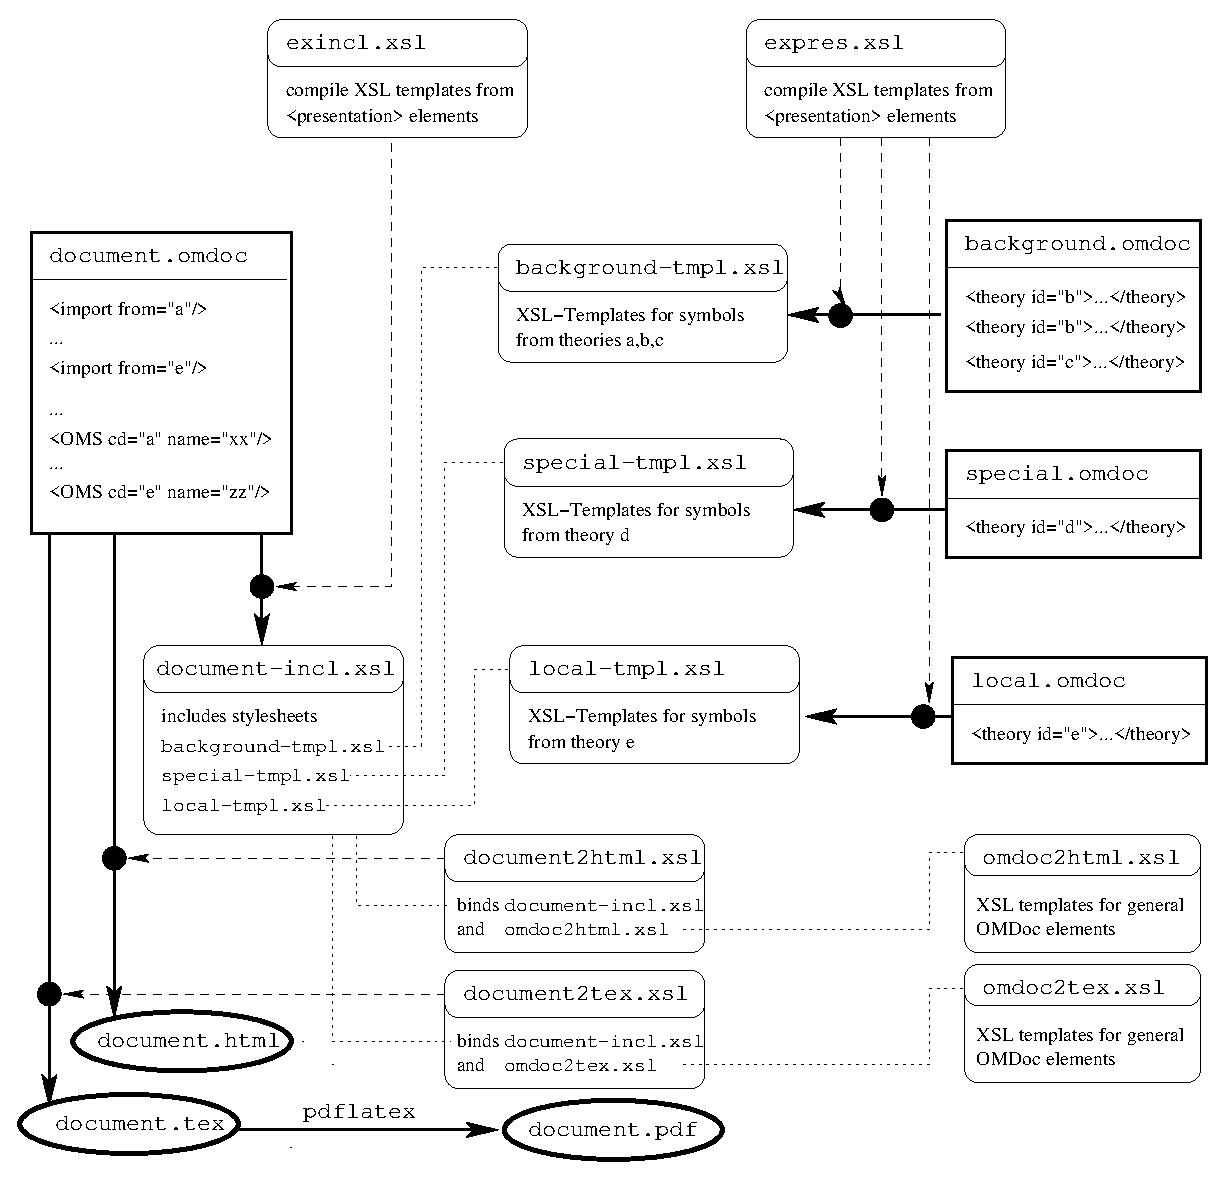
\includegraphics[width=10.5cm]{figures/presentation-arch}
\end{myfig}

Other processing architectures may be built up using
on-demand technologies, e.g. servlets, mediators, or web services, but will be
able to follow the same general pattern as our simpleminded implementation in
{\snippet{Makefiles}}.

We will make use of this general architecture based on extraction and linking via
{\xslt} style sheets in the transformation of {\omdoc} documents below.


\end{tsection}

\begin{tsection}[id=omdoctosys,short=Interfaces for Systems]{{\omdoc} Interfaces for Mathematical Software Systems}

  One of the original goals of the {\openmath}, {\cmathml} and {\omdoc} languages is to
  provide a communication language for mathematical software systems. The main idea behind
  this is to supply systems with interfaces to a universally accepted communication
  language standard (an {\indextoo{interlingua}}), and so achieve interoperability for $n$
  systems with only $2n$ translations instead of $n^2$. As we have seen in
  {\mysecref{math-objects}}, {\openmath} and {\cmathml} provide a good solution at the
  level of mathematical objects, which is sufficient for systems like {\twintoo{computer
      algebra}{system}s}. {\omdoc} adds the level of mathematical statements and theories
  to add support for automated reasoning systems and formal specification systems.

To make practical use of the {\omdoc} format as an interlingua, we have to support
building {\omdoc} interfaces. An {\xslt} style sheet is a simple way to come up with (the
input half) of an {\omdoc} interface.  A more efficient way would be to integrate an
{\xml}\twin{XML}{parser} directly into the system (suitable {\xml} parsers are readily
available for almost all programming languages nowadays).

Usually, the task of writing an {\xslt} style sheet for such a conversion is a
relatively simple task, since the input language of most mathematical software
system is isomorphic to a subset of {\omdoc}. This suggests the general strategy
of applying the necessary syntax transformations (this has to be supplied by the
style sheet author) on those {\omdoc} elements that carry system-relevant
information and transforming those that are not (e.g. Metadata and {\element{CMP}}
elements for most systems) into comments.  Much of the functionality is already
supplied by the style sheet {\snippetin{omdoc2sys.xsl}}, which need only be adapted to
know about the comment syntax. 

The task of translating an {\omdoc} document into system-specific input has two
sub-tasks. We will discuss them using the concrete example of the
{\snippetin{omdoc2pvs.xsl}} style sheet that transforms {\omdoc} documents to the input
language of the {\pvs} theorem prover~\cite{OwRu92}: The first task is to translate
elements at the statement- and theory level to the input language this is hand-coded by
supplying suitable templates for the {\omdoc} statement and theory elements in an
extension of the {\snippet{omdoc2sys.xsl}} style sheet. The second task is to translate
the formulae to the input language. Here, the system usually has a particular way of
expressing complex formulae like function applications and binding expressions; in the
concrete case of {\pvs}, function application uses a prefix function argument syntax, and
$n$-ary binding expressions, where the scope is separated by a colon from the variable
list. This information must also be encoded in respective templates for the
{\element[ns-elt=om]{OMA}}, {\element[ns-elt=om]{OMBIND}}, {\element[ns-elt=om]{OMV}}
elements from {\openmath} and the {\element[ns-elt=m]{apply}} and {\element[ns-elt=m]{ci}}
from {\cmathml}. For the symbol elements, we have to distinguish two cases: the
{\twintoo{predefined}{symbol}s} of the system language and the {\twintoo{object}{symbol}s}
that are introduced by the user to formalize a certain problem. In both cases, the
transformation procedure needs input on how these symbols are to be represented in the
system language. For the {\twintoo{object}{symbol}s} we assume that there are suitable
{\element{theory}} structures available, which declare them in {\element{symbol}}
elements, thus we can assume that these {\element{theory}} structures also contain
{\element{use}} elements with appropriate {\attribute{format}{use}} attribute in the
{\element{presentation}} elements for those symbols that need special representations in
the system language.  For the {\twintoo{predefined}{symbol}s} of the system language, we
assume the same.  To be able to transform an {\omdoc} document into system input, we need
a {\twintoo{language definition}{theory}}, i.e. an {\omdoc} document that contains a
{\element{theory}} which provides {\element{symbol}s} for all the predefined words of the
system language. This theory must also contain {\element{presentation}} elements with
{\element{use}} children specialized the input formats of all systems targeted for
communication.

\begin{lstlisting}[label=lst:system-language,
  caption={A {\element{symbol}} in a Language Definition Theory},
  index={symbol,presentation,style}]
<symbol name="sigmatype">
 <metadata>
   <dc:description>
     The dependent function type constructor is a binding operator. The source type is
     the type of the bound variable X, the target type is represented in the body.
   </dc:description>
 </metadata>
</symbol>

<presentation xml:id="pr-sigmatype" for="#sigmatype" role="binding">
  <style format="pvs">
    <text>[</text>
    <recurse select="*[2]/*"/><text> -&gt; </text><recurse select="*[3]"/>
    <text>]</text>
  </style>
  <style format="nuprl">
    <recurse select="*[2]/*"/><text> -&gt; </text><recurse select="*[3]"/>
  </style>
</presentation>
\end{lstlisting}

The other direction of the translation needed for communication is usually much
more complicated, since it involves parsing the often idiosyncratic output of
these systems. A better approach is to write specialized output generators for
these systems that directly generate {\omdoc} representations. This is usually a
rather simple thing to do, if the systems have internal data structures that
provide all the information required in {\omdoc}. It is sometimes a problem with
these systems that they only store the name of a symbol (logical constant) and not
its home theory. At other times, internal records of proofs in theorem provers are
optimized towards speed and not towards expressivity, so that some of the
information that had been discarded has to be recomputed for {\omdoc} output.

One of the practical problems that remains to be solved for interfaces between
mathematical software systems is that of semantic standardization of input
languages. For mathematical objects, this has been solved in principle by supplying a
theory level in the form of {\openmath} or {\omdoc} content dictionaries that define the
necessary mathematical concepts. For systems like theorem provers or theory development
environments we need to do the same with the logics underlying these systems. For an
effort to systematize logics into a hierarchy that fosters reuse and communication of
systems, based on a series of experiments of interfacing with the theorem proving systems
{\OMEGA}~\cite{BenzmuellerEtAl:otama97}, {\inka}~\cite{HuSe:itng96}, {\pvs}~\cite{OwRu92},
{\lambdaclam}~\cite{RicSmaGre:ppihol98}, {\tps}~\cite{AnBi:tatps96} and
{\coq}~\cite{CoqManual} see {\mysecref{logics}}
\end{tsection}

\begin{tsection}[id=omdoc2pres]{Presenting OMDoc to Humans}
We will now discuss the software infrastructure needed to transform {\omdoc}
documents into human-readable form in various formats. We speak of of {\omdoc}
{\defin{presentation}} for this task.

Due to the complex nature of {\omdoc} presentation, only part of it
can actually be performed by {\xslt} style sheets. For instance,
sub-tasks like reasoning about the prior knowledge of the user, or her
experience with certain proof techniques is clearly better left to
specialized applications. Our processing model is the following:
presenting an {\omdoc} is a two-phase process. 

The first phase is independent of the final output format (e.g. {\html}, {\mathml}, or
{\LaTeX}) and produces another {\omdoc} representation specialized to the respective user
or audience, taking into account prior knowledge, structural preferences, bandwidth and
time constraints, etc.  This phase usually generates a
{\twintoo{narrative-structured}{document}} from a knowledge-centered
one\twin{knowledge-centered}{document}. 

The second phase is a formatting process that can be extracted by {\xslt} style sheets
that transforms the resulting specialized document into the respective output format with
notational- and layout preferences of the audience. We will only discuss the second one
and refer the reader for ideas about the first process to systems like
P.rex~\cite{Fiedler:ddaoeo01,FiedlerHoracek:aietlp01}.

The presentation of the {\omdoc} document elements and statements is carried out by the
style sheets {\snippetin{omdoc2html.xsl}} for {\xhtml}, {\snippetin{omdoc2html.xsl}} for
{\xhtml}+{\mathml} and {\snippetin{omdoc2tex.xsl}} for {\LaTeX}. These style sheets are
divided into files according to the {\omdoc} modules and share a large common code base
{\snippetin{omdoc2share.xsl}}, basically the first two include the latter and only
redefine some format-specific options. For instance, {\snippetin{omdoc2share.xsl}}
supplies an infrastructure for {\indextoo{internationalization}} introduced in
{\mysecref{mtext}}. This allows to generate localized presentations of the {\omdoc}
documents, if enough information is present in the
{\twintoo{multilingual}{group}s}\twin{multilingual}{support}\twin{languages}{multiple} of
{\element{CMP}} elements. {\snippetin{omdoc2share.xsl}} takes a {\indextoo{parameter}}
{\snippetin{TargetLanguage}}, whose value can be a whitespace-separated preference list of
{\atwintoo{ISO}{639}{norm}} two-letter {\twintoo{country}{code}s}.  If
{\snippetin{TargetLanguage}} consists of a single entry, then the result will only contain
this language with gaps where the source document contains no suitable {\element{CMP}}.
Longer {\snippetin{TargetLanguage}} preference lists will generally result in more
complete, but {\twintoo{multilingual}{document}s}. Apart from the language-specific
elements in the source document, {\indextoo{localization}} also needs to know about the
presentation of certain keywords used in {\omdoc} markup, e.g.  the German ``Lemma'' and
the French ``Lemme'' for {\snippet{<assertion type="lemma">}}. This information is kept in
the keyword table {\snippet{lib/locale.xml}} in the {\omdoc} distribution, which contains
all the keywords necessary for presenting the {\omdoc} elements discussed so far.  An
alternative keyword table can be specified by the parameter {\index{parameter!{\xslt}}}
{\snippet{locale}}\index{locale@{\snippet{locale}} ({\xslt} parameter)}.
\end{tsection}
\end{tchapter}
%%% Local Variables: 
%%% mode: latex
%%% TeX-master: "omdoc"
%%% End: 

% LocalWords:  xsl saxon xalan xsltproc internet mozilla netscape cd xslt tmpl
% LocalWords:  expres omstyle ref exincl incl ab pvs rex pmml tex mtext Lemme
% LocalWords:  TargetLanguage ombind fol omdocIhtml xxx testIhtml pres pdflatex
% LocalWords:  ci changelog lib omdoctosys ns elt omdoc html CMP sys ary OMA
% LocalWords:  OMV sigmatype metadata recurse nuprl

% %%%%%%%%%%%%%%%%%%%%%%%%%%%%%%%%%%%%%%%%%%%%%%%%%%%%%%%%%%%%%%%%%%%%%%%%%
% This file is part of the LaTeX sources of the OMDoc 1.3 specification
% Copyright (c) 2016 Michael Kohlhase.
% Source at https://github.com/KWARC/OMDoc/tree/master/doc/spec
% This work is licensed by the Creative Commons Share-Alike license
% see http://creativecommons.org/licenses/by-sa/2.5/ for details
%%%%%%%%%%%%%%%%%%%%%%%%%%%%%%%%%%%%%%%%%%%%%%%%%%%%%%%%%%%%%%%%%%%%%%%%%

\begin{tchapter}[id=projects,short=Applications and Projects]{OMDoc Applications and Projects}

  This chapter presents a variety of applications and projects that use the {\omdoc}
  format or are related to it in a substantive way.  

  Apart from the projects directly reported here, the {\omdoc} format is used by the new
  research field of {\atwintoo{Mathematical}{Knowledge}{Management}} ({\sc mkm};
  cf.~\url{http://www.mkm-ig.org/}), which combines researchers in mathematics, computer
  science, and library science. We refer the reader to the proceedings of the annual
  {\sc{mkm}} conference~\cite{MKM01,MKM03,MKM04,MKM05,MKM06}.


\begin{tsection}[id=projeccts-intro]{Introduction}
  The text in the project descriptions has been contributed\footnote{If your {\omdoc}
    project is not represented here, please contact \url{m.kohlhase@jacobs-university.de} to arrange
    for inclusion in later editions of this book.} by the authors marked in the section
  headings, for questions about the projects or systems, please visit the web-sites given
  or contact the authors directly. Note that the material discussed in this chapter is
  under continuous development, and the account here only reflects the state of mid-2006,
  see \url{http://omdoc.org/projects/} for more and current information.


\begin{tsubsection}[id=projects-overview]{Overview}
  The {\omdoc} format as a whole and the applications mentioned above are supported by a
  variety of tools for creating, manipulating, and communicating {\omdoc} documents. We
  can distinguish four kinds of tools:

\begin{description}
\item[{\emph{Interfaces\index{interface} for Mathematical Software Systems}}] like
  automated theorem provers. These system are usually add-ins that interpret the internal
  representation of formalized mathematical objects in their host systems and recursively
  generate formal {\omdoc} documents as output and communication streams. Some of these
  systems also have input filters for {\omdoc} like the {\verifun} described in
  {\mysecref{verifun}}, but most rely on the {\omdoc} transformation to their native input
  syntax described in {\mysecref{omdoctosys}}.
\item[\emph{Invasive Editors\twin{invasive}{editor}}] i.e. are add-ins or modes that
  ``invade'' common general-purpose editing systems and specialize them to deal with the
  {\omdoc} format.  The {\omdoc} mode for the {\emacs} editor presented in
  {\mysecref{omdocmode}}, the {\cpoint} add-in for MS PowerPoint ({\mysecref{cpoint}}),
  the {\mathematica} notebook converter ({\mysecref{nb2omdoc}}), the {\sentido} plugin for
  {\mozilla}-based browsers, and the plugin for {\texmacs} ({\mysecref{texmacs-omega}})
  are examples for this kind of editor. They differ from simple output filter in providing
  editing functionality for {\omdoc} specific information.
\item[\emph{Human-Oriented Frontend Formats\atwin{human-oriented}{frontend}{format}}] for
  instance the {\qmath} project described in {\mysecref{qmath}} defines an interface
  language for a fragment of {\omdoc}, that is simpler to type by hand, and less verbose
  than the {\omdoc} that can be generated by the {\snippet{qmath}} parser. {\stex} defines
  a human-oriented format for {\omdoc} by extending the {\TeX/\LaTeX} with content markup
  primitives, so that it can be transformed to {\omdoc}. See {\mysecref{stex}} for
  details.
\item [\emph{Mathematical Knowledge Bases\atwin{mathematical}{knowledge}{base}}] The
  {\mbase} and {\maya} systems described in {\mysecsref{mbase}{maya}} are web-based
  mathematical knowledge bases that offer the infrastructure for a universal, distributed
  repository of formalized mathematics represented in the {\omdoc} format.
\end{description}
\end{tsubsection}

\begin{tsubsection}[id=omdoc-roles]{Application Roles of the OMDoc Format}

  The applications above support the utilization of the {\omdoc} format in several
  roles. Generally, {\omdoc} can used of as a
\begin{description}
\item[\emph{Communication Standard}\twin{communication}{standard}] between mechanized
reasoning systems.
\item[\emph{Data Format for Controlled Refinement}\twin{controlled}{refinement}] from
  informal presentation to formal specification of mathematical objects and theories.
  Basically, an informal textual presentation can first be marked up, by making its
  structure\twin{structure}{discourse} explicit (classifying text fragments as
  definitions, theorems, proofs, linking text, and their relations), and then formalizing
  the textually given mathematical knowledge in logical formulae (by adding
  {\element{FMP}} elements; see {\mychapref{mtxt}}).
\item[\emph{Document Preparation Language}\twin{document}{preparation language}.]  The
  {\omdoc} format makes the large-scale document- and conceptual structures explicit and
  facilitates maintenance on this level. Individual documents can be encoded as
  lightweight narrative structures, which can directly be transformed to e.g.
  {\xhtml}+{\mathml} or {\LaTeX}, which can in turn be published on the Internet.
\item[\emph{Basis for Individualized (Interactive)
    Documents}\twin{document}{interactive}\twin{individualized}{document}.] Personalized
  {\twintoo{narrative}{structure}s} can be generated from {\mbase} content making use of
  the {\twintoo{conceptual}{structure}} encoded in {\mbase} together with a user model.
  For instance, the {\mmiss}, {\MathDox}, and {\activemath} projects described in
  {\myseclref{MMiSS}{activemath}} use the {\omdoc} infrastructure in an educational
  setting. They make use of the content-orientation and the explicit structural markup of
  the mathematical knowledge to generate on the fly specialized learning materials that
  are adapted to the students prior knowledge, learning goals, and notational tastes.
\item[\emph{Interface for Proof Presentation\twin{proof}{presentation}}.] As the proof
  part of {\omdoc} allows small-grained interleaving of formal ({\element{FMP}}) and
  textual ({\element{CMP}}) presentations in multiple languages (see
  e.g.~\cite{HuangFiedler:pvip97,Fiedler:uacatp99}).
\end{description}
\end{tsubsection}

\end{tsection}

\begin{projectdescription}
  %%%%%%%%%%%%%%%%%%%%%%%%%%%%%%%%%%%%%%%%%%%%%%%%%%%%%%%%%%%%%%%%%%%%%%%%%
% This file is part of the LaTeX sources of the OMDoc 1.3 specifiation
% Copyright (c) 2006 Christoph Lange
% This work is licensed by the Creative Commons Share-Alike license
% see http://creativecommons.org/licenses/by-sa/2.5/ for details
\svnInfo $Id: main.tex 8453 2009-08-04 09:58:26Z kohlhase $
\svnKeyword $HeadURL: https://svn.omdoc.org/repos/omdoc/branches/omdoc-1.3/doc/spec/projects/swim/main.tex $
%%%%%%%%%%%%%%%%%%%%%%%%%%%%%%%%%%%%%%%%%%%%%%%%%%%%%%%%%%%%%%%%%%%%%%%%%

\section{{\swim} -- An OMDoc-based Semantic Wiki}
\begin{project}{swim}{http://kwarc.eecs.iu-bremen.de/projects/swim}
\pauthors{Christoph Lange\and Michael Kohlhase}
\pinstitute{Computer Science, International University Bremen}
\end{project}

{\swim} is a semantic wiki for collaboratively building, editing and browsing a
mathematical knowledge base of {\omdoc} theories. Our long-term objective is to develop a
software that facilitates the creation of a shared, public collection of mathematical
knowledge and serves work groups of mathematicians as a tool for collaborative development
of new theories.  Even though the work reported here was initially motivated by solving
the MKM author's dilemma~\cite{KohKoh:cdad04}, we contend that the new application area
MKM can also contribute to the development of semantic wikis.

Technically, {\swim} is based on the semantic wiki engine
\scsys{IkeWiki}~\cite{schaffert06:ikewiki}, which was chosen because of its
modular design, its rich semantic web infrastructure, its user assistance for
annotations, and its orientation towards
learning~\cite{schaffert06:learning-with-semantic-wikis}.

\subsection{Semantic Wikis}

A wiki~\cite{LeuCun01:wikiway} is a web server
application that allows users to browse, create, and edit hyperlinked pages in a web
browser, usually using a simple text syntax.  In contrast to most content management
systems, wiki pages are accessible via an URL containing their title.  A new page can be
created by linking from an existent page to the page to be created.  This link will then
lead to an edit form.  Usually, anyone is allowed to edit pages on a wiki, but access can
be restricted.  Other characteristics of wikis include permanent storage of old page
versions (with facilities to display differences between two versions and to restore a
certain version), notification about recent changes, and full-text search.

Semantic
wikis~\cite{voelkel06:semanticwikistateoftheart,TolPas06:wikis-semantic-hypermedia}
enhance wikis by Semantic Web technologies, such as {\rdf}~\cite{LasSwi:rdf99} or
ontologies.  Usually one page represents one concept from a real-world domain, which has a
type, possibly some metadata, and typed links to other concepts.  For example, a link from
a wiki page about ``Life, the Universe and Everything'' to another page about Douglas
Adams could be typed as ``is author of''.  In terms of {\rdf}, this can be expressed by the
following subject--predicate--object triple,

\[
(\mbox{``Douglas Adams''},\;\mbox{isAuthorOf},\;\mbox{``Life, the Universe and
Everything''})
\]

where the \textit{isAuthorOf} relation would be defined in an ontology.  These links are
usually displayed in a navigation box next to the page contents. Semantic wikis only deal
with wiki text, not with mathematics, though some allow to embed mathematical formulae as
presentational-only {\TeX}.

{\swim} encourages users to collaborate: Non-mathematicians can collaborate in creating a
``Wikipedia of mathematics'' by compiling the knowledge available so far, while scientists
can collaboratively develop new theories.  Users get an immediate reward for many of their
contributions: Once they specify the type of a page or relations of one page to another,
this information will be displayed in a box of navigation links.  We intend to make the
data created in {\swim} usable for external services by offering an export facility for
{\omdoc} documents and by integrating them into {\swim}.  Mathematicians developing
theories will be assisted to retain an overview of theory dependencies in order not to
break them.  Social software services will further utilize the semantic information
available from the theories and from tracking the user interaction log (``Who did what on
which page when?'').  User feedback to pages can be extended to social bookmarking, which
is ``the practice of saving bookmarks [of Internet resources] to a public web site and
`tagging' them with keywords.''~\cite{lomas05:social-bookmarking} The more users tag a
certain resource, the higher a social bookmarking service will rank it.

The enhancements of the data model semantic wikis bring along --- compared to traditional
wikis --- are already present in the {\omdoc} format, so that an {\omdoc}-based wiki only
needs to operationalize their underlying meaning. For example, typed links, which are
implemented via an extension to the wiki syntax in \scsys{Semantic
  MediaWiki}~\cite{voelkel06:semanticwikipedia} or editable through a separate editor in
\scsys{IkeWiki}~\cite{schaffert06:ikewiki}, are implemented by means of the \texttt{for}
attribute to {\omdoc}'s elements (e.g.\ \texttt{<example for="\#id-of-assertion">}).
{\swim} makes them editable easily and visualizes them adequately.  A semantic wiki
targeted at mathematics must ensure that dependencies between concepts are preserved.
Results in this area will be interesting for non-mathematical semantic wikis as well,
especially when they support higher levels of formalization such as ontologies.

\subsection{Design of {\swim}}

\subsubsection{Concepts and Relations}

The smallest unit that can be displayed, edited, linked to, or archived in a wiki is a
page. In a semantic wiki, it usually describes one {\emph{concept}}, including its
properties and its relations to other concepts.  While standalone {\omdoc} documents can
contain more than one theory, is is important to keep pages small in a wiki to improve the
effectivity of usage.  Furthermore, usual semantic wikis only store and display metadata
and typed links per page; {\swim} does too.\footnote{Semantic information will only be
  considered on the theory and statement levels of {\omdoc} --- directly or through
  reasoning in the case of transitive closures ---, not on the object level.}  Users are
strongly encouraged to define at most one theory per wiki page and to roll out
non-constitutive statements (see {\mysecref{statements-constitutive}}) to separate pages,
referencing their context theory.  As constitutive statements cannot exist without an
enclosing theory, but as, on the other hand, we want each wiki page to form a valid
document, we introduced a new element {\element[ns-elt=swim]{page}}, which can be a child
of an {\element{omdoc}} element and which has the same content model as a
{\element{theory}} element --- in particular, it can hold several theory-constitutive
statements and connect them to their context theory.
\begin{wrapfigure}{r}{8cm}
  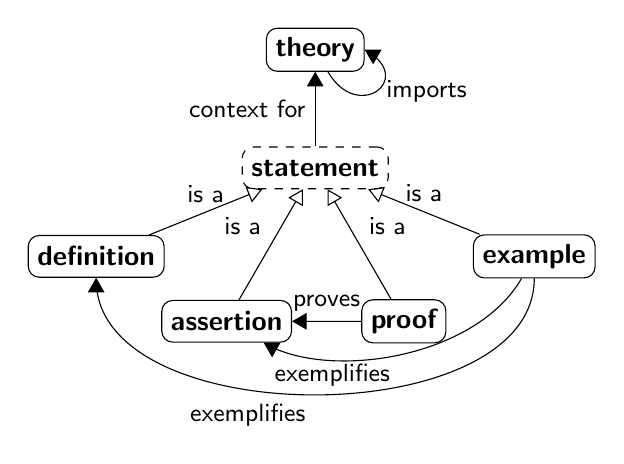
\begin{tikzpicture}[scale=1.5,thin,font=\sffamily,>=triangle 60]
    \tikzstyle{concept}=[font=\sffamily\bfseries,draw,minimum height=3.5ex,rounded corners]
    \tikzstyle{every path}=[font=\small\sffamily];
    \node[concept] (t) at (0,1) {theory};
    \node[concept,dashed] (s) at (0,0) {\itshape statement};
    \node[concept] (d) at +(-158:2.0cm) {definition};
    \begin{scope}[shift={(d)}]% control point for e->d
      \coordinate (da) at +(-90:1.5cm);% relative to s, not to a!
    \end{scope}
    \node[concept] (a) at +(-120:1.5cm) {assertion};
    \begin{scope}[shift={(a)}]% control point for e->a
      \coordinate (aa) at +(-30:1cm);% relative to s, not to a!
    \end{scope}
    \node[concept] (p) at +(-60:1.5cm) {proof};
    \node[concept] (e) at +(-22:2.0cm) {example};
    \draw[->] (t.-60) .. controls +(-60:0.5cm) and +(-30:0.5cm) .. node[right]
    {imports} (t.east);
    \draw[->] (s) -- node[left] {context for} (t);
    \draw[-open triangle 60] (d) -- node[above] {is a} (s);
    \draw[-open triangle 60] (a) -- node[above left] {is a} (s);
    \draw[-open triangle 60] (p) -- node[above right] {is a} (s);
    \draw[-open triangle 60] (e) -- node[above] {is a} (s);
    \draw[->] (p) -- node[above] {proves} (a);
    \draw[->] (e) ..
    controls +(-120:1cm)
    and (aa) ..
    node[below left] {exemplifies} (a);
    \draw[->] (e) ..
    controls +(-90:1.5cm)
    and (da) ..
    node[below left] {exemplifies} (d);
  \end{tikzpicture}
  \caption{Subset of {\omdoc}'s system ontology}\vspace*{-.5cm}
\end{wrapfigure}
{\omdoc}'s system ontology has been partly coded in OWL-DL and imported to the wiki's {\rdf}
store, which is implemented using the Jena Semantic Web Framework for
Java~\cite{URL:jena:web}. Theories as well as statements of any type form concepts, and
the most important relations between those concepts are extracted from the {\omdoc} pages
on saving and then stored as {\rdf} triples.  These relations include:
\begin{itemize}
\item The import relation between theories
\item The relation of a statement to its context theory
\item The relation of an example to the statement it exemplifies
\item The relation of a proof to the assertion it proves
\end{itemize}
It is planned to also take relations given by user interaction into consideration, such as
``Who edited which page when?'', and to combine ontology-defined relations and user
relations.  For example, a metric estimating the {\emph{degree of difficulty}} of a page,
calculated by counting the questions on the discussion page, could be implemented.
Furthermore, the user can specify taxonomic relations, which cannot be stated explicitly
in {\omdoc}, such as (``all differentiable functions are continuous''), as annotations in
an ontology language like {\rdf} Schema or {\owl}.

\subsubsection{User Interface and Interaction Model}

Pages can be rendered to XHTML plus presentational MathML using the transformations
described in {\mychapref{transform-xsl}}. There is also a browsable source code view, which is
useful for documents that are not written in textbook style.

Not only will the user be able to navigate along the dependency graph, she will also be
able to {\emph{interact}} with the system: she will be asked whether she wants to explore
the theories required as dependencies in further detail.

Suppose that the user is currently reading the page containing the theory {\snippet{ring}}
from the elementary algebra example from {\mychapref{dg-elal}}. In this case the wiki will
not only display navigation links to the direct dependencies {\snippet{group}} and
{\snippet{monoid}}, but it will also provide unobtrusive buttons that allow the user to
give one of the commands in {\myfigref{gui-showdeps}}. Not only the last case will be
recorded --- the others are interesting as well for \emph{social bookmarking}.  For
example, if many users requested a theory $t$ to be explained, the system could default to
display not only the direct dependencies but also the level-two dependencies, for it seems
that $t$ is too difficult for only being explained shallowly.

\begin{myfig}{gui-showdeps}{The command buttons to navigate along the dependencies}
  \begin{minipage}{8cm}
\begin{description}
\item[{\bf{No, thanks!}}] ``{\emph{I already know group and monoid.}}''
\item[{\bf{Explain}}] ``{\emph{Please show me group and monoid, I want to learn about
      ring's prerequisites.}}'' --- group and monoid will be displayed.
\item[{\bf{Explore}}] ``{\emph{Please show me {\emph{all}} prerequisites for ring.}}'' ---
  group, monoid, and semigroup, are opened in separate windows or serialized into one
  page.
\item[{\bf{Suspend}}] ``{\emph{I want to know about group and monoid, but only later.}}''
  --- {\swim} keeps a notice in the user's profile that she wants to read group and monoid
  sometime.  Reminder links to suspended theories are shown on a separate navigation bar.
\end{description}
\end{minipage}\quad
\begin{minipage}{2.5cm}
  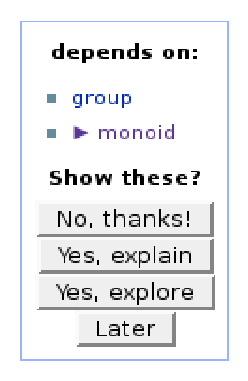
\includegraphics[width=2.5cm]{projects/swim/gui-showdeps}
\end{minipage}
\end{myfig}

\subsubsection{Further work}

Further work on {\swim} will concentrate on integrating a lightweight
management of change process.  Second, while the wiki is yet a user-friendly
\emph{browser}, there is still a demand for assisting users to \emph{edit}
{\omdoc}.  To this end, the {\qmath} preprocessor (see {\mysecref{qmath}}) will
be integrated into {\swim}.  Mathematical objects entered as {\qmath} will be
kept in this syntax for display in the edit form, but they will be converted to
{\omdoc} for rendering for presentation and when pages are exported to another
application.

%%% Local Variables: 
%%% mode: stex
%%% TeX-master: "../../omdoc"
%%% End: 

% LocalWords:  matwebsearch Ioan Sucan nC dx dy dt runningex XPointer ns attr
% LocalWords:  mq anyorder xmlns domainofapplication bvar ci cn eq OAI API da
% LocalWords:  Lange CPoint wikis dateness parseable isAuthorOf MediaWiki omdoc
% LocalWords:  aa wiki's Wiki wiki IkeWiki JA hypermedia elt semithick pres dg
% LocalWords:  elal gui showdeps qmath stex metadata wiki's scheint mir kein zu
% LocalWords:  Gegensatz sein

\end{projectdescription}

\begin{projectdescription}
  %%%%%%%%%%%%%%%%%%%%%%%%%%%%%%%%%%%%%%%%%%%%%%%%%%%%%%%%%%%%%%%%%%%%%%%%%
% This file is part of the LaTeX sources of the OMDoc 1.3 specifiation
% Copyright (c) 2006 Christoph Lange
% This work is licensed by the Creative Commons Share-Alike license
% see http://creativecommons.org/licenses/by-sa/2.5/ for details
\svnInfo $Id: main.tex 8453 2009-08-04 09:58:26Z kohlhase $
\svnKeyword $HeadURL: https://svn.omdoc.org/repos/omdoc/branches/omdoc-1.3/doc/spec/projects/swim/main.tex $
%%%%%%%%%%%%%%%%%%%%%%%%%%%%%%%%%%%%%%%%%%%%%%%%%%%%%%%%%%%%%%%%%%%%%%%%%

\section{{\swim} -- An OMDoc-based Semantic Wiki}
\begin{project}{swim}{http://kwarc.eecs.iu-bremen.de/projects/swim}
\pauthors{Christoph Lange\and Michael Kohlhase}
\pinstitute{Computer Science, International University Bremen}
\end{project}

{\swim} is a semantic wiki for collaboratively building, editing and browsing a
mathematical knowledge base of {\omdoc} theories. Our long-term objective is to develop a
software that facilitates the creation of a shared, public collection of mathematical
knowledge and serves work groups of mathematicians as a tool for collaborative development
of new theories.  Even though the work reported here was initially motivated by solving
the MKM author's dilemma~\cite{KohKoh:cdad04}, we contend that the new application area
MKM can also contribute to the development of semantic wikis.

Technically, {\swim} is based on the semantic wiki engine
\scsys{IkeWiki}~\cite{schaffert06:ikewiki}, which was chosen because of its
modular design, its rich semantic web infrastructure, its user assistance for
annotations, and its orientation towards
learning~\cite{schaffert06:learning-with-semantic-wikis}.

\subsection{Semantic Wikis}

A wiki~\cite{LeuCun01:wikiway} is a web server
application that allows users to browse, create, and edit hyperlinked pages in a web
browser, usually using a simple text syntax.  In contrast to most content management
systems, wiki pages are accessible via an URL containing their title.  A new page can be
created by linking from an existent page to the page to be created.  This link will then
lead to an edit form.  Usually, anyone is allowed to edit pages on a wiki, but access can
be restricted.  Other characteristics of wikis include permanent storage of old page
versions (with facilities to display differences between two versions and to restore a
certain version), notification about recent changes, and full-text search.

Semantic
wikis~\cite{voelkel06:semanticwikistateoftheart,TolPas06:wikis-semantic-hypermedia}
enhance wikis by Semantic Web technologies, such as {\rdf}~\cite{LasSwi:rdf99} or
ontologies.  Usually one page represents one concept from a real-world domain, which has a
type, possibly some metadata, and typed links to other concepts.  For example, a link from
a wiki page about ``Life, the Universe and Everything'' to another page about Douglas
Adams could be typed as ``is author of''.  In terms of {\rdf}, this can be expressed by the
following subject--predicate--object triple,

\[
(\mbox{``Douglas Adams''},\;\mbox{isAuthorOf},\;\mbox{``Life, the Universe and
Everything''})
\]

where the \textit{isAuthorOf} relation would be defined in an ontology.  These links are
usually displayed in a navigation box next to the page contents. Semantic wikis only deal
with wiki text, not with mathematics, though some allow to embed mathematical formulae as
presentational-only {\TeX}.

{\swim} encourages users to collaborate: Non-mathematicians can collaborate in creating a
``Wikipedia of mathematics'' by compiling the knowledge available so far, while scientists
can collaboratively develop new theories.  Users get an immediate reward for many of their
contributions: Once they specify the type of a page or relations of one page to another,
this information will be displayed in a box of navigation links.  We intend to make the
data created in {\swim} usable for external services by offering an export facility for
{\omdoc} documents and by integrating them into {\swim}.  Mathematicians developing
theories will be assisted to retain an overview of theory dependencies in order not to
break them.  Social software services will further utilize the semantic information
available from the theories and from tracking the user interaction log (``Who did what on
which page when?'').  User feedback to pages can be extended to social bookmarking, which
is ``the practice of saving bookmarks [of Internet resources] to a public web site and
`tagging' them with keywords.''~\cite{lomas05:social-bookmarking} The more users tag a
certain resource, the higher a social bookmarking service will rank it.

The enhancements of the data model semantic wikis bring along --- compared to traditional
wikis --- are already present in the {\omdoc} format, so that an {\omdoc}-based wiki only
needs to operationalize their underlying meaning. For example, typed links, which are
implemented via an extension to the wiki syntax in \scsys{Semantic
  MediaWiki}~\cite{voelkel06:semanticwikipedia} or editable through a separate editor in
\scsys{IkeWiki}~\cite{schaffert06:ikewiki}, are implemented by means of the \texttt{for}
attribute to {\omdoc}'s elements (e.g.\ \texttt{<example for="\#id-of-assertion">}).
{\swim} makes them editable easily and visualizes them adequately.  A semantic wiki
targeted at mathematics must ensure that dependencies between concepts are preserved.
Results in this area will be interesting for non-mathematical semantic wikis as well,
especially when they support higher levels of formalization such as ontologies.

\subsection{Design of {\swim}}

\subsubsection{Concepts and Relations}

The smallest unit that can be displayed, edited, linked to, or archived in a wiki is a
page. In a semantic wiki, it usually describes one {\emph{concept}}, including its
properties and its relations to other concepts.  While standalone {\omdoc} documents can
contain more than one theory, is is important to keep pages small in a wiki to improve the
effectivity of usage.  Furthermore, usual semantic wikis only store and display metadata
and typed links per page; {\swim} does too.\footnote{Semantic information will only be
  considered on the theory and statement levels of {\omdoc} --- directly or through
  reasoning in the case of transitive closures ---, not on the object level.}  Users are
strongly encouraged to define at most one theory per wiki page and to roll out
non-constitutive statements (see {\mysecref{statements-constitutive}}) to separate pages,
referencing their context theory.  As constitutive statements cannot exist without an
enclosing theory, but as, on the other hand, we want each wiki page to form a valid
document, we introduced a new element {\element[ns-elt=swim]{page}}, which can be a child
of an {\element{omdoc}} element and which has the same content model as a
{\element{theory}} element --- in particular, it can hold several theory-constitutive
statements and connect them to their context theory.
\begin{wrapfigure}{r}{8cm}
  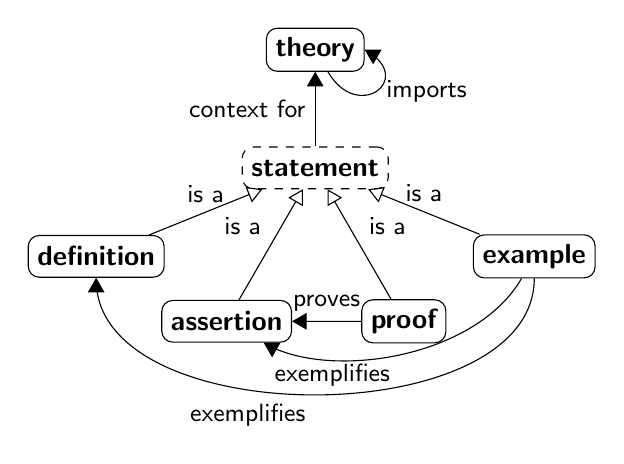
\begin{tikzpicture}[scale=1.5,thin,font=\sffamily,>=triangle 60]
    \tikzstyle{concept}=[font=\sffamily\bfseries,draw,minimum height=3.5ex,rounded corners]
    \tikzstyle{every path}=[font=\small\sffamily];
    \node[concept] (t) at (0,1) {theory};
    \node[concept,dashed] (s) at (0,0) {\itshape statement};
    \node[concept] (d) at +(-158:2.0cm) {definition};
    \begin{scope}[shift={(d)}]% control point for e->d
      \coordinate (da) at +(-90:1.5cm);% relative to s, not to a!
    \end{scope}
    \node[concept] (a) at +(-120:1.5cm) {assertion};
    \begin{scope}[shift={(a)}]% control point for e->a
      \coordinate (aa) at +(-30:1cm);% relative to s, not to a!
    \end{scope}
    \node[concept] (p) at +(-60:1.5cm) {proof};
    \node[concept] (e) at +(-22:2.0cm) {example};
    \draw[->] (t.-60) .. controls +(-60:0.5cm) and +(-30:0.5cm) .. node[right]
    {imports} (t.east);
    \draw[->] (s) -- node[left] {context for} (t);
    \draw[-open triangle 60] (d) -- node[above] {is a} (s);
    \draw[-open triangle 60] (a) -- node[above left] {is a} (s);
    \draw[-open triangle 60] (p) -- node[above right] {is a} (s);
    \draw[-open triangle 60] (e) -- node[above] {is a} (s);
    \draw[->] (p) -- node[above] {proves} (a);
    \draw[->] (e) ..
    controls +(-120:1cm)
    and (aa) ..
    node[below left] {exemplifies} (a);
    \draw[->] (e) ..
    controls +(-90:1.5cm)
    and (da) ..
    node[below left] {exemplifies} (d);
  \end{tikzpicture}
  \caption{Subset of {\omdoc}'s system ontology}\vspace*{-.5cm}
\end{wrapfigure}
{\omdoc}'s system ontology has been partly coded in OWL-DL and imported to the wiki's {\rdf}
store, which is implemented using the Jena Semantic Web Framework for
Java~\cite{URL:jena:web}. Theories as well as statements of any type form concepts, and
the most important relations between those concepts are extracted from the {\omdoc} pages
on saving and then stored as {\rdf} triples.  These relations include:
\begin{itemize}
\item The import relation between theories
\item The relation of a statement to its context theory
\item The relation of an example to the statement it exemplifies
\item The relation of a proof to the assertion it proves
\end{itemize}
It is planned to also take relations given by user interaction into consideration, such as
``Who edited which page when?'', and to combine ontology-defined relations and user
relations.  For example, a metric estimating the {\emph{degree of difficulty}} of a page,
calculated by counting the questions on the discussion page, could be implemented.
Furthermore, the user can specify taxonomic relations, which cannot be stated explicitly
in {\omdoc}, such as (``all differentiable functions are continuous''), as annotations in
an ontology language like {\rdf} Schema or {\owl}.

\subsubsection{User Interface and Interaction Model}

Pages can be rendered to XHTML plus presentational MathML using the transformations
described in {\mychapref{transform-xsl}}. There is also a browsable source code view, which is
useful for documents that are not written in textbook style.

Not only will the user be able to navigate along the dependency graph, she will also be
able to {\emph{interact}} with the system: she will be asked whether she wants to explore
the theories required as dependencies in further detail.

Suppose that the user is currently reading the page containing the theory {\snippet{ring}}
from the elementary algebra example from {\mychapref{dg-elal}}. In this case the wiki will
not only display navigation links to the direct dependencies {\snippet{group}} and
{\snippet{monoid}}, but it will also provide unobtrusive buttons that allow the user to
give one of the commands in {\myfigref{gui-showdeps}}. Not only the last case will be
recorded --- the others are interesting as well for \emph{social bookmarking}.  For
example, if many users requested a theory $t$ to be explained, the system could default to
display not only the direct dependencies but also the level-two dependencies, for it seems
that $t$ is too difficult for only being explained shallowly.

\begin{myfig}{gui-showdeps}{The command buttons to navigate along the dependencies}
  \begin{minipage}{8cm}
\begin{description}
\item[{\bf{No, thanks!}}] ``{\emph{I already know group and monoid.}}''
\item[{\bf{Explain}}] ``{\emph{Please show me group and monoid, I want to learn about
      ring's prerequisites.}}'' --- group and monoid will be displayed.
\item[{\bf{Explore}}] ``{\emph{Please show me {\emph{all}} prerequisites for ring.}}'' ---
  group, monoid, and semigroup, are opened in separate windows or serialized into one
  page.
\item[{\bf{Suspend}}] ``{\emph{I want to know about group and monoid, but only later.}}''
  --- {\swim} keeps a notice in the user's profile that she wants to read group and monoid
  sometime.  Reminder links to suspended theories are shown on a separate navigation bar.
\end{description}
\end{minipage}\quad
\begin{minipage}{2.5cm}
  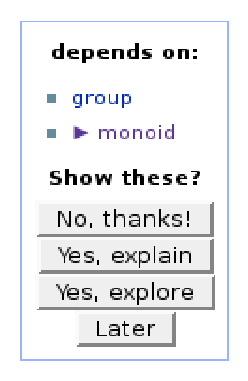
\includegraphics[width=2.5cm]{projects/swim/gui-showdeps}
\end{minipage}
\end{myfig}

\subsubsection{Further work}

Further work on {\swim} will concentrate on integrating a lightweight
management of change process.  Second, while the wiki is yet a user-friendly
\emph{browser}, there is still a demand for assisting users to \emph{edit}
{\omdoc}.  To this end, the {\qmath} preprocessor (see {\mysecref{qmath}}) will
be integrated into {\swim}.  Mathematical objects entered as {\qmath} will be
kept in this syntax for display in the edit form, but they will be converted to
{\omdoc} for rendering for presentation and when pages are exported to another
application.

%%% Local Variables: 
%%% mode: stex
%%% TeX-master: "../../omdoc"
%%% End: 

% LocalWords:  matwebsearch Ioan Sucan nC dx dy dt runningex XPointer ns attr
% LocalWords:  mq anyorder xmlns domainofapplication bvar ci cn eq OAI API da
% LocalWords:  Lange CPoint wikis dateness parseable isAuthorOf MediaWiki omdoc
% LocalWords:  aa wiki's Wiki wiki IkeWiki JA hypermedia elt semithick pres dg
% LocalWords:  elal gui showdeps qmath stex metadata wiki's scheint mir kein zu
% LocalWords:  Gegensatz sein

\end{projectdescription}

\begin{projectdescription}
  %%%%%%%%%%%%%%%%%%%%%%%%%%%%%%%%%%%%%%%%%%%%%%%%%%%%%%%%%%%%%%%%%%%%%%%%%
% This file is part of the LaTeX sources of the OMDoc 1.3 specifiation
% Copyright (c) 2006 Christoph Lange
% This work is licensed by the Creative Commons Share-Alike license
% see http://creativecommons.org/licenses/by-sa/2.5/ for details
\svnInfo $Id: main.tex 8453 2009-08-04 09:58:26Z kohlhase $
\svnKeyword $HeadURL: https://svn.omdoc.org/repos/omdoc/branches/omdoc-1.3/doc/spec/projects/swim/main.tex $
%%%%%%%%%%%%%%%%%%%%%%%%%%%%%%%%%%%%%%%%%%%%%%%%%%%%%%%%%%%%%%%%%%%%%%%%%

\section{{\swim} -- An OMDoc-based Semantic Wiki}
\begin{project}{swim}{http://kwarc.eecs.iu-bremen.de/projects/swim}
\pauthors{Christoph Lange\and Michael Kohlhase}
\pinstitute{Computer Science, International University Bremen}
\end{project}

{\swim} is a semantic wiki for collaboratively building, editing and browsing a
mathematical knowledge base of {\omdoc} theories. Our long-term objective is to develop a
software that facilitates the creation of a shared, public collection of mathematical
knowledge and serves work groups of mathematicians as a tool for collaborative development
of new theories.  Even though the work reported here was initially motivated by solving
the MKM author's dilemma~\cite{KohKoh:cdad04}, we contend that the new application area
MKM can also contribute to the development of semantic wikis.

Technically, {\swim} is based on the semantic wiki engine
\scsys{IkeWiki}~\cite{schaffert06:ikewiki}, which was chosen because of its
modular design, its rich semantic web infrastructure, its user assistance for
annotations, and its orientation towards
learning~\cite{schaffert06:learning-with-semantic-wikis}.

\subsection{Semantic Wikis}

A wiki~\cite{LeuCun01:wikiway} is a web server
application that allows users to browse, create, and edit hyperlinked pages in a web
browser, usually using a simple text syntax.  In contrast to most content management
systems, wiki pages are accessible via an URL containing their title.  A new page can be
created by linking from an existent page to the page to be created.  This link will then
lead to an edit form.  Usually, anyone is allowed to edit pages on a wiki, but access can
be restricted.  Other characteristics of wikis include permanent storage of old page
versions (with facilities to display differences between two versions and to restore a
certain version), notification about recent changes, and full-text search.

Semantic
wikis~\cite{voelkel06:semanticwikistateoftheart,TolPas06:wikis-semantic-hypermedia}
enhance wikis by Semantic Web technologies, such as {\rdf}~\cite{LasSwi:rdf99} or
ontologies.  Usually one page represents one concept from a real-world domain, which has a
type, possibly some metadata, and typed links to other concepts.  For example, a link from
a wiki page about ``Life, the Universe and Everything'' to another page about Douglas
Adams could be typed as ``is author of''.  In terms of {\rdf}, this can be expressed by the
following subject--predicate--object triple,

\[
(\mbox{``Douglas Adams''},\;\mbox{isAuthorOf},\;\mbox{``Life, the Universe and
Everything''})
\]

where the \textit{isAuthorOf} relation would be defined in an ontology.  These links are
usually displayed in a navigation box next to the page contents. Semantic wikis only deal
with wiki text, not with mathematics, though some allow to embed mathematical formulae as
presentational-only {\TeX}.

{\swim} encourages users to collaborate: Non-mathematicians can collaborate in creating a
``Wikipedia of mathematics'' by compiling the knowledge available so far, while scientists
can collaboratively develop new theories.  Users get an immediate reward for many of their
contributions: Once they specify the type of a page or relations of one page to another,
this information will be displayed in a box of navigation links.  We intend to make the
data created in {\swim} usable for external services by offering an export facility for
{\omdoc} documents and by integrating them into {\swim}.  Mathematicians developing
theories will be assisted to retain an overview of theory dependencies in order not to
break them.  Social software services will further utilize the semantic information
available from the theories and from tracking the user interaction log (``Who did what on
which page when?'').  User feedback to pages can be extended to social bookmarking, which
is ``the practice of saving bookmarks [of Internet resources] to a public web site and
`tagging' them with keywords.''~\cite{lomas05:social-bookmarking} The more users tag a
certain resource, the higher a social bookmarking service will rank it.

The enhancements of the data model semantic wikis bring along --- compared to traditional
wikis --- are already present in the {\omdoc} format, so that an {\omdoc}-based wiki only
needs to operationalize their underlying meaning. For example, typed links, which are
implemented via an extension to the wiki syntax in \scsys{Semantic
  MediaWiki}~\cite{voelkel06:semanticwikipedia} or editable through a separate editor in
\scsys{IkeWiki}~\cite{schaffert06:ikewiki}, are implemented by means of the \texttt{for}
attribute to {\omdoc}'s elements (e.g.\ \texttt{<example for="\#id-of-assertion">}).
{\swim} makes them editable easily and visualizes them adequately.  A semantic wiki
targeted at mathematics must ensure that dependencies between concepts are preserved.
Results in this area will be interesting for non-mathematical semantic wikis as well,
especially when they support higher levels of formalization such as ontologies.

\subsection{Design of {\swim}}

\subsubsection{Concepts and Relations}

The smallest unit that can be displayed, edited, linked to, or archived in a wiki is a
page. In a semantic wiki, it usually describes one {\emph{concept}}, including its
properties and its relations to other concepts.  While standalone {\omdoc} documents can
contain more than one theory, is is important to keep pages small in a wiki to improve the
effectivity of usage.  Furthermore, usual semantic wikis only store and display metadata
and typed links per page; {\swim} does too.\footnote{Semantic information will only be
  considered on the theory and statement levels of {\omdoc} --- directly or through
  reasoning in the case of transitive closures ---, not on the object level.}  Users are
strongly encouraged to define at most one theory per wiki page and to roll out
non-constitutive statements (see {\mysecref{statements-constitutive}}) to separate pages,
referencing their context theory.  As constitutive statements cannot exist without an
enclosing theory, but as, on the other hand, we want each wiki page to form a valid
document, we introduced a new element {\element[ns-elt=swim]{page}}, which can be a child
of an {\element{omdoc}} element and which has the same content model as a
{\element{theory}} element --- in particular, it can hold several theory-constitutive
statements and connect them to their context theory.
\begin{wrapfigure}{r}{8cm}
  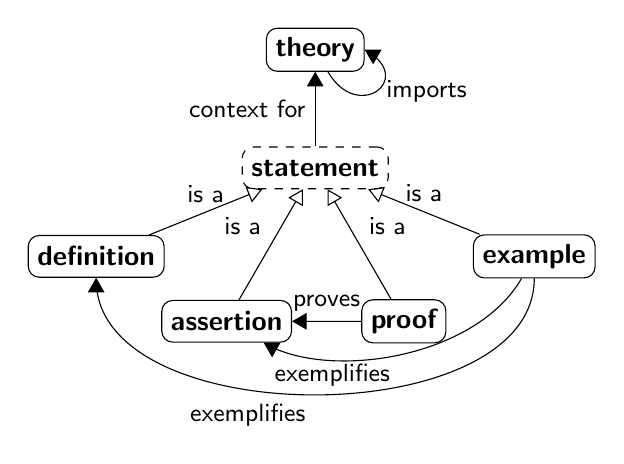
\begin{tikzpicture}[scale=1.5,thin,font=\sffamily,>=triangle 60]
    \tikzstyle{concept}=[font=\sffamily\bfseries,draw,minimum height=3.5ex,rounded corners]
    \tikzstyle{every path}=[font=\small\sffamily];
    \node[concept] (t) at (0,1) {theory};
    \node[concept,dashed] (s) at (0,0) {\itshape statement};
    \node[concept] (d) at +(-158:2.0cm) {definition};
    \begin{scope}[shift={(d)}]% control point for e->d
      \coordinate (da) at +(-90:1.5cm);% relative to s, not to a!
    \end{scope}
    \node[concept] (a) at +(-120:1.5cm) {assertion};
    \begin{scope}[shift={(a)}]% control point for e->a
      \coordinate (aa) at +(-30:1cm);% relative to s, not to a!
    \end{scope}
    \node[concept] (p) at +(-60:1.5cm) {proof};
    \node[concept] (e) at +(-22:2.0cm) {example};
    \draw[->] (t.-60) .. controls +(-60:0.5cm) and +(-30:0.5cm) .. node[right]
    {imports} (t.east);
    \draw[->] (s) -- node[left] {context for} (t);
    \draw[-open triangle 60] (d) -- node[above] {is a} (s);
    \draw[-open triangle 60] (a) -- node[above left] {is a} (s);
    \draw[-open triangle 60] (p) -- node[above right] {is a} (s);
    \draw[-open triangle 60] (e) -- node[above] {is a} (s);
    \draw[->] (p) -- node[above] {proves} (a);
    \draw[->] (e) ..
    controls +(-120:1cm)
    and (aa) ..
    node[below left] {exemplifies} (a);
    \draw[->] (e) ..
    controls +(-90:1.5cm)
    and (da) ..
    node[below left] {exemplifies} (d);
  \end{tikzpicture}
  \caption{Subset of {\omdoc}'s system ontology}\vspace*{-.5cm}
\end{wrapfigure}
{\omdoc}'s system ontology has been partly coded in OWL-DL and imported to the wiki's {\rdf}
store, which is implemented using the Jena Semantic Web Framework for
Java~\cite{URL:jena:web}. Theories as well as statements of any type form concepts, and
the most important relations between those concepts are extracted from the {\omdoc} pages
on saving and then stored as {\rdf} triples.  These relations include:
\begin{itemize}
\item The import relation between theories
\item The relation of a statement to its context theory
\item The relation of an example to the statement it exemplifies
\item The relation of a proof to the assertion it proves
\end{itemize}
It is planned to also take relations given by user interaction into consideration, such as
``Who edited which page when?'', and to combine ontology-defined relations and user
relations.  For example, a metric estimating the {\emph{degree of difficulty}} of a page,
calculated by counting the questions on the discussion page, could be implemented.
Furthermore, the user can specify taxonomic relations, which cannot be stated explicitly
in {\omdoc}, such as (``all differentiable functions are continuous''), as annotations in
an ontology language like {\rdf} Schema or {\owl}.

\subsubsection{User Interface and Interaction Model}

Pages can be rendered to XHTML plus presentational MathML using the transformations
described in {\mychapref{transform-xsl}}. There is also a browsable source code view, which is
useful for documents that are not written in textbook style.

Not only will the user be able to navigate along the dependency graph, she will also be
able to {\emph{interact}} with the system: she will be asked whether she wants to explore
the theories required as dependencies in further detail.

Suppose that the user is currently reading the page containing the theory {\snippet{ring}}
from the elementary algebra example from {\mychapref{dg-elal}}. In this case the wiki will
not only display navigation links to the direct dependencies {\snippet{group}} and
{\snippet{monoid}}, but it will also provide unobtrusive buttons that allow the user to
give one of the commands in {\myfigref{gui-showdeps}}. Not only the last case will be
recorded --- the others are interesting as well for \emph{social bookmarking}.  For
example, if many users requested a theory $t$ to be explained, the system could default to
display not only the direct dependencies but also the level-two dependencies, for it seems
that $t$ is too difficult for only being explained shallowly.

\begin{myfig}{gui-showdeps}{The command buttons to navigate along the dependencies}
  \begin{minipage}{8cm}
\begin{description}
\item[{\bf{No, thanks!}}] ``{\emph{I already know group and monoid.}}''
\item[{\bf{Explain}}] ``{\emph{Please show me group and monoid, I want to learn about
      ring's prerequisites.}}'' --- group and monoid will be displayed.
\item[{\bf{Explore}}] ``{\emph{Please show me {\emph{all}} prerequisites for ring.}}'' ---
  group, monoid, and semigroup, are opened in separate windows or serialized into one
  page.
\item[{\bf{Suspend}}] ``{\emph{I want to know about group and monoid, but only later.}}''
  --- {\swim} keeps a notice in the user's profile that she wants to read group and monoid
  sometime.  Reminder links to suspended theories are shown on a separate navigation bar.
\end{description}
\end{minipage}\quad
\begin{minipage}{2.5cm}
  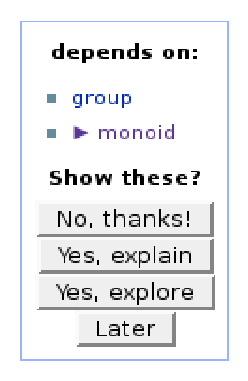
\includegraphics[width=2.5cm]{projects/swim/gui-showdeps}
\end{minipage}
\end{myfig}

\subsubsection{Further work}

Further work on {\swim} will concentrate on integrating a lightweight
management of change process.  Second, while the wiki is yet a user-friendly
\emph{browser}, there is still a demand for assisting users to \emph{edit}
{\omdoc}.  To this end, the {\qmath} preprocessor (see {\mysecref{qmath}}) will
be integrated into {\swim}.  Mathematical objects entered as {\qmath} will be
kept in this syntax for display in the edit form, but they will be converted to
{\omdoc} for rendering for presentation and when pages are exported to another
application.

%%% Local Variables: 
%%% mode: stex
%%% TeX-master: "../../omdoc"
%%% End: 

% LocalWords:  matwebsearch Ioan Sucan nC dx dy dt runningex XPointer ns attr
% LocalWords:  mq anyorder xmlns domainofapplication bvar ci cn eq OAI API da
% LocalWords:  Lange CPoint wikis dateness parseable isAuthorOf MediaWiki omdoc
% LocalWords:  aa wiki's Wiki wiki IkeWiki JA hypermedia elt semithick pres dg
% LocalWords:  elal gui showdeps qmath stex metadata wiki's scheint mir kein zu
% LocalWords:  Gegensatz sein

\end{projectdescription}

\begin{projectdescription}
  %%%%%%%%%%%%%%%%%%%%%%%%%%%%%%%%%%%%%%%%%%%%%%%%%%%%%%%%%%%%%%%%%%%%%%%%%
% This file is part of the LaTeX sources of the OMDoc 1.3 specifiation
% Copyright (c) 2006 Christoph Lange
% This work is licensed by the Creative Commons Share-Alike license
% see http://creativecommons.org/licenses/by-sa/2.5/ for details
\svnInfo $Id: main.tex 8453 2009-08-04 09:58:26Z kohlhase $
\svnKeyword $HeadURL: https://svn.omdoc.org/repos/omdoc/branches/omdoc-1.3/doc/spec/projects/swim/main.tex $
%%%%%%%%%%%%%%%%%%%%%%%%%%%%%%%%%%%%%%%%%%%%%%%%%%%%%%%%%%%%%%%%%%%%%%%%%

\section{{\swim} -- An OMDoc-based Semantic Wiki}
\begin{project}{swim}{http://kwarc.eecs.iu-bremen.de/projects/swim}
\pauthors{Christoph Lange\and Michael Kohlhase}
\pinstitute{Computer Science, International University Bremen}
\end{project}

{\swim} is a semantic wiki for collaboratively building, editing and browsing a
mathematical knowledge base of {\omdoc} theories. Our long-term objective is to develop a
software that facilitates the creation of a shared, public collection of mathematical
knowledge and serves work groups of mathematicians as a tool for collaborative development
of new theories.  Even though the work reported here was initially motivated by solving
the MKM author's dilemma~\cite{KohKoh:cdad04}, we contend that the new application area
MKM can also contribute to the development of semantic wikis.

Technically, {\swim} is based on the semantic wiki engine
\scsys{IkeWiki}~\cite{schaffert06:ikewiki}, which was chosen because of its
modular design, its rich semantic web infrastructure, its user assistance for
annotations, and its orientation towards
learning~\cite{schaffert06:learning-with-semantic-wikis}.

\subsection{Semantic Wikis}

A wiki~\cite{LeuCun01:wikiway} is a web server
application that allows users to browse, create, and edit hyperlinked pages in a web
browser, usually using a simple text syntax.  In contrast to most content management
systems, wiki pages are accessible via an URL containing their title.  A new page can be
created by linking from an existent page to the page to be created.  This link will then
lead to an edit form.  Usually, anyone is allowed to edit pages on a wiki, but access can
be restricted.  Other characteristics of wikis include permanent storage of old page
versions (with facilities to display differences between two versions and to restore a
certain version), notification about recent changes, and full-text search.

Semantic
wikis~\cite{voelkel06:semanticwikistateoftheart,TolPas06:wikis-semantic-hypermedia}
enhance wikis by Semantic Web technologies, such as {\rdf}~\cite{LasSwi:rdf99} or
ontologies.  Usually one page represents one concept from a real-world domain, which has a
type, possibly some metadata, and typed links to other concepts.  For example, a link from
a wiki page about ``Life, the Universe and Everything'' to another page about Douglas
Adams could be typed as ``is author of''.  In terms of {\rdf}, this can be expressed by the
following subject--predicate--object triple,

\[
(\mbox{``Douglas Adams''},\;\mbox{isAuthorOf},\;\mbox{``Life, the Universe and
Everything''})
\]

where the \textit{isAuthorOf} relation would be defined in an ontology.  These links are
usually displayed in a navigation box next to the page contents. Semantic wikis only deal
with wiki text, not with mathematics, though some allow to embed mathematical formulae as
presentational-only {\TeX}.

{\swim} encourages users to collaborate: Non-mathematicians can collaborate in creating a
``Wikipedia of mathematics'' by compiling the knowledge available so far, while scientists
can collaboratively develop new theories.  Users get an immediate reward for many of their
contributions: Once they specify the type of a page or relations of one page to another,
this information will be displayed in a box of navigation links.  We intend to make the
data created in {\swim} usable for external services by offering an export facility for
{\omdoc} documents and by integrating them into {\swim}.  Mathematicians developing
theories will be assisted to retain an overview of theory dependencies in order not to
break them.  Social software services will further utilize the semantic information
available from the theories and from tracking the user interaction log (``Who did what on
which page when?'').  User feedback to pages can be extended to social bookmarking, which
is ``the practice of saving bookmarks [of Internet resources] to a public web site and
`tagging' them with keywords.''~\cite{lomas05:social-bookmarking} The more users tag a
certain resource, the higher a social bookmarking service will rank it.

The enhancements of the data model semantic wikis bring along --- compared to traditional
wikis --- are already present in the {\omdoc} format, so that an {\omdoc}-based wiki only
needs to operationalize their underlying meaning. For example, typed links, which are
implemented via an extension to the wiki syntax in \scsys{Semantic
  MediaWiki}~\cite{voelkel06:semanticwikipedia} or editable through a separate editor in
\scsys{IkeWiki}~\cite{schaffert06:ikewiki}, are implemented by means of the \texttt{for}
attribute to {\omdoc}'s elements (e.g.\ \texttt{<example for="\#id-of-assertion">}).
{\swim} makes them editable easily and visualizes them adequately.  A semantic wiki
targeted at mathematics must ensure that dependencies between concepts are preserved.
Results in this area will be interesting for non-mathematical semantic wikis as well,
especially when they support higher levels of formalization such as ontologies.

\subsection{Design of {\swim}}

\subsubsection{Concepts and Relations}

The smallest unit that can be displayed, edited, linked to, or archived in a wiki is a
page. In a semantic wiki, it usually describes one {\emph{concept}}, including its
properties and its relations to other concepts.  While standalone {\omdoc} documents can
contain more than one theory, is is important to keep pages small in a wiki to improve the
effectivity of usage.  Furthermore, usual semantic wikis only store and display metadata
and typed links per page; {\swim} does too.\footnote{Semantic information will only be
  considered on the theory and statement levels of {\omdoc} --- directly or through
  reasoning in the case of transitive closures ---, not on the object level.}  Users are
strongly encouraged to define at most one theory per wiki page and to roll out
non-constitutive statements (see {\mysecref{statements-constitutive}}) to separate pages,
referencing their context theory.  As constitutive statements cannot exist without an
enclosing theory, but as, on the other hand, we want each wiki page to form a valid
document, we introduced a new element {\element[ns-elt=swim]{page}}, which can be a child
of an {\element{omdoc}} element and which has the same content model as a
{\element{theory}} element --- in particular, it can hold several theory-constitutive
statements and connect them to their context theory.
\begin{wrapfigure}{r}{8cm}
  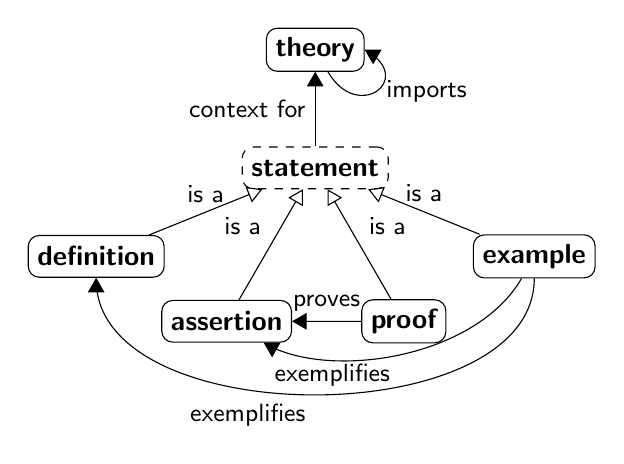
\begin{tikzpicture}[scale=1.5,thin,font=\sffamily,>=triangle 60]
    \tikzstyle{concept}=[font=\sffamily\bfseries,draw,minimum height=3.5ex,rounded corners]
    \tikzstyle{every path}=[font=\small\sffamily];
    \node[concept] (t) at (0,1) {theory};
    \node[concept,dashed] (s) at (0,0) {\itshape statement};
    \node[concept] (d) at +(-158:2.0cm) {definition};
    \begin{scope}[shift={(d)}]% control point for e->d
      \coordinate (da) at +(-90:1.5cm);% relative to s, not to a!
    \end{scope}
    \node[concept] (a) at +(-120:1.5cm) {assertion};
    \begin{scope}[shift={(a)}]% control point for e->a
      \coordinate (aa) at +(-30:1cm);% relative to s, not to a!
    \end{scope}
    \node[concept] (p) at +(-60:1.5cm) {proof};
    \node[concept] (e) at +(-22:2.0cm) {example};
    \draw[->] (t.-60) .. controls +(-60:0.5cm) and +(-30:0.5cm) .. node[right]
    {imports} (t.east);
    \draw[->] (s) -- node[left] {context for} (t);
    \draw[-open triangle 60] (d) -- node[above] {is a} (s);
    \draw[-open triangle 60] (a) -- node[above left] {is a} (s);
    \draw[-open triangle 60] (p) -- node[above right] {is a} (s);
    \draw[-open triangle 60] (e) -- node[above] {is a} (s);
    \draw[->] (p) -- node[above] {proves} (a);
    \draw[->] (e) ..
    controls +(-120:1cm)
    and (aa) ..
    node[below left] {exemplifies} (a);
    \draw[->] (e) ..
    controls +(-90:1.5cm)
    and (da) ..
    node[below left] {exemplifies} (d);
  \end{tikzpicture}
  \caption{Subset of {\omdoc}'s system ontology}\vspace*{-.5cm}
\end{wrapfigure}
{\omdoc}'s system ontology has been partly coded in OWL-DL and imported to the wiki's {\rdf}
store, which is implemented using the Jena Semantic Web Framework for
Java~\cite{URL:jena:web}. Theories as well as statements of any type form concepts, and
the most important relations between those concepts are extracted from the {\omdoc} pages
on saving and then stored as {\rdf} triples.  These relations include:
\begin{itemize}
\item The import relation between theories
\item The relation of a statement to its context theory
\item The relation of an example to the statement it exemplifies
\item The relation of a proof to the assertion it proves
\end{itemize}
It is planned to also take relations given by user interaction into consideration, such as
``Who edited which page when?'', and to combine ontology-defined relations and user
relations.  For example, a metric estimating the {\emph{degree of difficulty}} of a page,
calculated by counting the questions on the discussion page, could be implemented.
Furthermore, the user can specify taxonomic relations, which cannot be stated explicitly
in {\omdoc}, such as (``all differentiable functions are continuous''), as annotations in
an ontology language like {\rdf} Schema or {\owl}.

\subsubsection{User Interface and Interaction Model}

Pages can be rendered to XHTML plus presentational MathML using the transformations
described in {\mychapref{transform-xsl}}. There is also a browsable source code view, which is
useful for documents that are not written in textbook style.

Not only will the user be able to navigate along the dependency graph, she will also be
able to {\emph{interact}} with the system: she will be asked whether she wants to explore
the theories required as dependencies in further detail.

Suppose that the user is currently reading the page containing the theory {\snippet{ring}}
from the elementary algebra example from {\mychapref{dg-elal}}. In this case the wiki will
not only display navigation links to the direct dependencies {\snippet{group}} and
{\snippet{monoid}}, but it will also provide unobtrusive buttons that allow the user to
give one of the commands in {\myfigref{gui-showdeps}}. Not only the last case will be
recorded --- the others are interesting as well for \emph{social bookmarking}.  For
example, if many users requested a theory $t$ to be explained, the system could default to
display not only the direct dependencies but also the level-two dependencies, for it seems
that $t$ is too difficult for only being explained shallowly.

\begin{myfig}{gui-showdeps}{The command buttons to navigate along the dependencies}
  \begin{minipage}{8cm}
\begin{description}
\item[{\bf{No, thanks!}}] ``{\emph{I already know group and monoid.}}''
\item[{\bf{Explain}}] ``{\emph{Please show me group and monoid, I want to learn about
      ring's prerequisites.}}'' --- group and monoid will be displayed.
\item[{\bf{Explore}}] ``{\emph{Please show me {\emph{all}} prerequisites for ring.}}'' ---
  group, monoid, and semigroup, are opened in separate windows or serialized into one
  page.
\item[{\bf{Suspend}}] ``{\emph{I want to know about group and monoid, but only later.}}''
  --- {\swim} keeps a notice in the user's profile that she wants to read group and monoid
  sometime.  Reminder links to suspended theories are shown on a separate navigation bar.
\end{description}
\end{minipage}\quad
\begin{minipage}{2.5cm}
  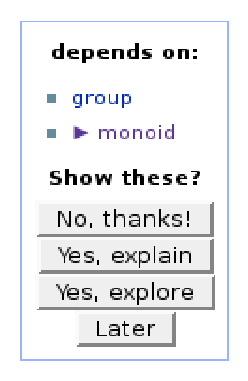
\includegraphics[width=2.5cm]{projects/swim/gui-showdeps}
\end{minipage}
\end{myfig}

\subsubsection{Further work}

Further work on {\swim} will concentrate on integrating a lightweight
management of change process.  Second, while the wiki is yet a user-friendly
\emph{browser}, there is still a demand for assisting users to \emph{edit}
{\omdoc}.  To this end, the {\qmath} preprocessor (see {\mysecref{qmath}}) will
be integrated into {\swim}.  Mathematical objects entered as {\qmath} will be
kept in this syntax for display in the edit form, but they will be converted to
{\omdoc} for rendering for presentation and when pages are exported to another
application.

%%% Local Variables: 
%%% mode: stex
%%% TeX-master: "../../omdoc"
%%% End: 

% LocalWords:  matwebsearch Ioan Sucan nC dx dy dt runningex XPointer ns attr
% LocalWords:  mq anyorder xmlns domainofapplication bvar ci cn eq OAI API da
% LocalWords:  Lange CPoint wikis dateness parseable isAuthorOf MediaWiki omdoc
% LocalWords:  aa wiki's Wiki wiki IkeWiki JA hypermedia elt semithick pres dg
% LocalWords:  elal gui showdeps qmath stex metadata wiki's scheint mir kein zu
% LocalWords:  Gegensatz sein

\end{projectdescription}

\begin{projectdescription}
  %%%%%%%%%%%%%%%%%%%%%%%%%%%%%%%%%%%%%%%%%%%%%%%%%%%%%%%%%%%%%%%%%%%%%%%%%
% This file is part of the LaTeX sources of the OMDoc 1.3 specifiation
% Copyright (c) 2006 Bernd Krieg-Brueckner, Achim Mahnke
% This work is licensed by the Creative Commons Share-Alike license
% see http://creativecommons.org/licenses/by-sa/2.5/ for details
\svnInfo $Id: mmiss.tex 8453 2009-08-04 09:58:26Z kohlhase $
\svnKeyword $HeadURL: https://svn.omdoc.org/repos/omdoc/branches/omdoc-1.3/doc/spec/projects/semrelations/mmiss.tex $
%%%%%%%%%%%%%%%%%%%%%%%%%%%%%%%%%%%%%%%%%%%%%%%%%%%%%%%%%%%%%%%%%%%%%%%%%

\section{Semantic Interrelation and Change Management}
\begin{project}{MMiSS}{http://www.mmiss.de}
\pauthors{Bernd Krieg-Br{\"u}ckner\and  Achim Mahnke}
\pinstitute{Computer Science, University of Bremen, Germany}
\end{project}
The corpus of electronically available mathematical knowledge increases rapidly.  Usually,
mathematical objects are embedded in and related to different kinds of documents like
articles, books, or lecture material, the domain of which can be different from
mathematics, e.g., engineering or computer science. Therefore, maintaining high-quality
mathematical knowledge becomes a non-trivial engineering task for teams of authors.

In this scenario, sharing\twin{document}{sharing} and reuse\twin{document}{reuse} is the
key to efficient development. Unfortunately, while there has been a large body of research
concerning the sharing and reuse of program developments, sharing and reuse of documents
has until now been mainly done by little more than cut and paste.  However, to ensure
sustainable development, i.e. continuous long-term usability of the contents, sharing and
reuse needs to be supported by tools and methods taking into account the semantic
structure of the document. In developing these methods and tools we can benefit from the
experience in {\atwin{formal}{software}{development}} and associated support tools.

We address this problem by providing a methodology to specify coherence and consistency of
documents by interrelation of semantic terms and structural entities, supported by a tool
for fine-grained {\twintoo{version}{control}} and {\twintoo{configuration}{management}}
including {\twintoo{change}{management}}. Semantic
interrelation\twin{semantic}{interrelation} explicates the meaning lying behind the
textual content, and relates the semantic concepts within and across documents by means of
an ontology. To allow change management, each document is structured in-the-small.  Each
document corresponds to a package, and packages may be structured in-the-large using
folders and import relations. The ideas and methods explained here have been developed in
the \MMISS{} project which aimed at the construction of a multi-media Internet-based
adaptive educational system (see \cite{MMISS-WADT03,SemInter-DELFI04,MMISS-TechReport04}).

\subsection{Semantic Interrelation Via Ontologies}

Ontologies\index{ontology} provide the means for establishing a semantic structure. An
ontology is a formal explicit description of concepts in a domain of discourse. The
{\MMISS\LaTeX} package for ontologies provides a set of easy-to-use macros for the
declaration of ontologies in {\LaTeX} documents. They are used to {\emph{declare}} the
ontology of semantic terms used in a document, in a prelude up front. This
{\emph{specification}} of the document contains at least a rigorous hierarchical structure
of the terminology (a taxonomy, the {\emph{signature}} of the document), and may be seen
as an elaborate index structure. Moreover, relations between terms may be defined for more
semantic interrelation.

The ontology serves a dual purpose --- just as the specification of an
{\atwintoo{abstract}{data}{type}} in program development: it specifies the content to be
expected in the body of the document in an abstract, yet precise, manner --- the content
developers {\twintoo{requirement}{specification}}; and it specifies the content for
reference from the outside --- the user's perspective, who may then view the body of the
document as a black box. The content developer will use the {\MMISS\LaTeX} {\snippet{Def}}
command to specify the {\emph{defining}} occurrence of a promised term, as for an
index. Using the {\twintoo{structuring}{in-the-large}} facilities via packages, the
external user may then refer between documents using various kinds of {\emph{reference}}
commands, as the content developer may within a document.


  \begin{figure}[t]
    \begin{minipage}[b]{.6\textwidth}
      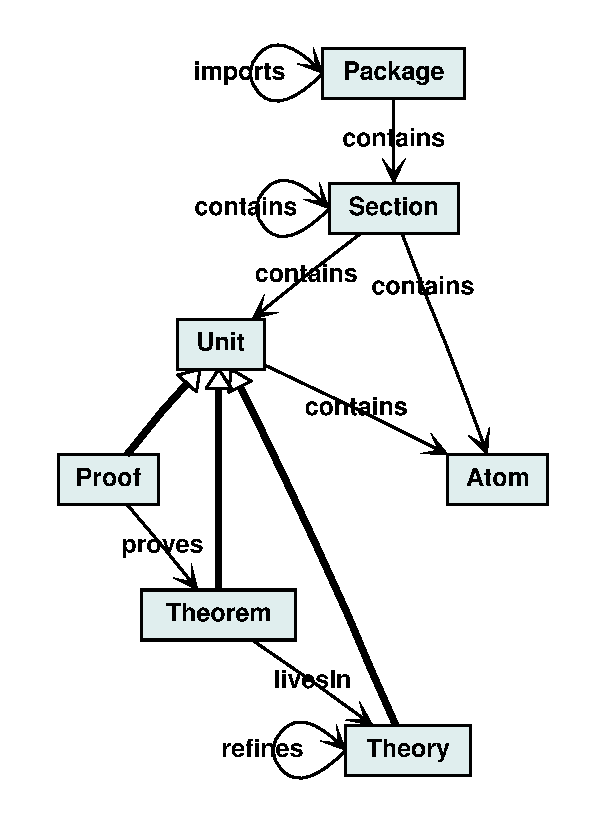
\includegraphics[width=.5\textwidth]{projects/semrelations/systems_onto_short}
    \end{minipage}
    \hspace*{-1cm}
    \begin{minipage}[b]{.4\textwidth}
      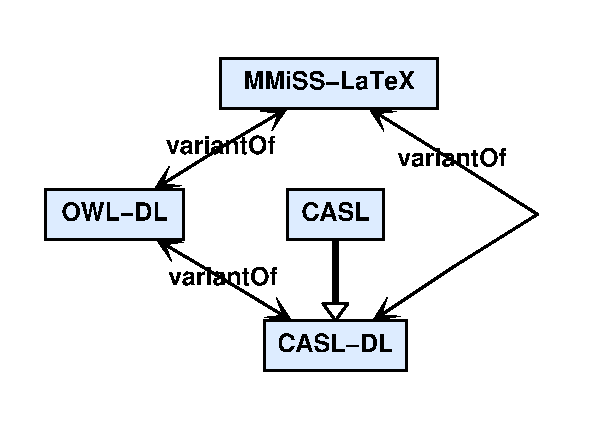
\includegraphics[width=1.1\textwidth]{projects/semrelations/onto_formalisms}
  \end{minipage}
  \caption{(a) Parts of the System's Ontology (b) Formalism variants}\label{fig:semrel-systems_onto}
\end{figure}

The next section will show, how we can explore this domain ontology --- supplied by the
author --- in order to capture semantic relations between document parts and use these
relations for supporting a management of change for mathematical documents.

\subsection{Change Management}

The notion of \emph{change management} is used for the maintenance and preservation of
consistency and completeness of a development during its evolution.  More precisely, we
want to have a {\twintoo{consistent}{configuration}} in which all versions are compatible
and there are no cyclic definitions or proofs.  At the same time, it should be a
{\twintoo{complete}{configuration}}: there should be no dangling forward references.

Such notions are well-known for formal languages. In contrast, natural language used for
writing teaching material does not usually possess a well-defined semantics, and the
notion of consistency is arguable.  Different authors may postulate different requirements
on the material in order to regard it as being consistent.  The existence of a
user-defined ontology helps a great deal to check references. However, we can make even
better use of the information contained in the ontology.

\paragraph{The System's Ontology}

The aim is to allow change management with regard to consistency and completeness
requirements defined by the user in terms of an ontology. In order to unify this approach
with the structural consistency and completeness properties introduced above, we express
the {\twintoo{document}{structure}}, originally defined by a document type definition, as
an ontology, the so-called \emph{System's Ontology} (see
Fig.~\ref{fig:semrel-systems_onto}a).  It defines the following relations between
structural elements of documents:
\begin{description}
\item [{\snippet{comprises}}] An obvious structuring mechanism is nesting of individual
  parts of a document, leading to the contains relation. The contains relation is part of
  a family of {\snippet{comprises}} relations that share common properties.
\item [{\snippet{reliesOn}}] A family of {\snippet{reliesOn}} relations reflects the
  various dependencies between different parts of a document.  For example, a theorem
  \emph{lives in} a theory, or proof \emph{proves} a theorem.
\item [{\snippet{pointsTo}}] The family of {\snippet{pointsTo}} relations is very similar,
  and relates references with the defining occurrence of a semantic term.
\item [{\snippet{variantOf}}] Another structuring relation is introduced by
  variants. Parts of a document may e.g. be written in various languages which gives rise
  to a {\snippet{variantOf}} relation between these document parts and their constituents;
  it is an equivalence relation.
\end{description}

It is now rather straightforward to formulate consistency and completeness rules in terms
of invariants of these relations. Formulating these invariants as formal rules will enable
us to implement a generic and flexible {\twintoo{change}{management}} that keeps track of
the invariants and informs the user about violations when a previously consistent document
has been revised, leading to various kinds of error (e.g. for {\snippet{reliesOn}}
relations) or warning messages (e.g. for {\snippet{pointsTo}} relations).


\paragraph{Properties of Interactions between Structuring Mechanisms.}
This approach also allows us to lift relations to structuring mechanisms allowing more
modular and localized change management.  For example, relating the {\snippet{comprises}}
and {\snippet{reliesOn}} relations allows us to formalize invariants regarding the closure
of document parts with respect to the {\snippet{reliesOn}} relation: We can require that
there is a proof for each theorem in a package.  Furthermore, if two structural entities
are related by {\snippet{reliesOn}}, their relation is propagated along the
{\snippet{comprises}} relation towards the root of the hierarchy of nested structural
entities, such that (for a theorem $T$ a proof $P$, and sections $A, B$):

\begin{description}
\item[] $B$ contains $P$ \& $A$ contains $T$ \& $P$ proves $T \Rightarrow B$
  {\snippet{reliesOn}} $A$.
\end{description}

% \[\text{B contains P and A contains T and P proves T, then
%         B reliesOn A.}
% \]

If the user changes section $A$, the repository will only need to check all sections that
$A$ relies on (such as $B$ here) for invariants, and not the whole document. However, in
contrast to formal developments as in e.g. the MAYA system \cite{AH-05-a}, there is no
rigorous requirement that a document should obey all the rules.  There may be good
reasons, for instance, to present first a "light-weight" introduction to all notions
introduced in a section before giving the detailed definitions. In this particular case,
one would want to introduce forward pointers to the definitions rather than making the
definitions rely on the introduction; thus the rules are covered.

In any case, the more structure there is, the better the chances are for preserving
consistency and completeness; any investment in introducing more {\snippet{reliesOn}}
relations, for example, will pay off eventually. The change management will observe
whether revisions by the user will affect these relations and, depending on the user's
preferences, emit corresponding warnings.

The aim is to allow users to specify individual notions of consistency by formulating the
rules that the relations should obey. This should be possible for the relations between
the particular (predefined) structuring mechanisms, but also in general between semantic
terms of the user's own ontology. Our work in this direction will rely on the methods and
tools provided by the {\hets} system (see {\mysecref{hets}}).

\subsection{Variants}

The concept of {\indextoo{variant}s} adds a new dimension to hierarchically
{\twintoo{structured}{document}s}.  The idea is to maintain and manage different variants
of structural entities (document subtrees) which represent the same information in
different ways --- variants are meant to glue them together.

Managing different natural language variants in parallel is an obvious example.  Another
one is the formalism variant which denotes the particular formalism in which a formal
content part like a theorem or a definition is expressed. Considering ontology development
itself, for example, we propose to use variants to maintain different formal
representations for the same semantic concept together with its documentation.
Figure~\ref{fig:semrel-systems_onto}b shows the possible variants for declaring ontology
components (see \cite{WOSE-2004} for details).

The \MMISS{} repository provides functions to store and retrieve these structural variants
by means of specifications for selecting particular variants for editing or presentation.

\subsection{Relations to {\omdoc}}

{\omdoc} provides modules for marking up the knowledge structure and the narrative
structure of mathematical documents. \MMISS{} combines these two viewpoints by giving
means for structuring the document contents (which constitutes the narrative structure) and
for specifying the incorporated knowledge by use of ontologies. Therefore, we have
implemented an export of \MMISS{} documents to (content and narrative) {\omdoc} documents
and vice versa.

% LocalWords:  MMiSS Bernd Krieg ckner Achim Mahnke multi reliesOn pointsTo
% LocalWords:  variantOf hets subtrees versa

\end{projectdescription}

\begin{projectdescription}
  %%%%%%%%%%%%%%%%%%%%%%%%%%%%%%%%%%%%%%%%%%%%%%%%%%%%%%%%%%%%%%%%%%%%%%%%%
% This file is part of the LaTeX sources of the OMDoc 1.3 specifiation
% Copyright (c) 2006 A.M. Cohen, H. Cuypers, E. Reinaldo Barreiro
% This work is licensed by the Creative Commons Share-Alike license
% see http://creativecommons.org/licenses/by-sa/2.5/ for details
\svnInfo $Id: mathdox2.tex 8453 2009-08-04 09:58:26Z kohlhase $
\svnKeyword $HeadURL: https://svn.omdoc.org/repos/omdoc/branches/omdoc-1.3/doc/spec/projects/mathdox/mathdox2.tex $
%%%%%%%%%%%%%%%%%%%%%%%%%%%%%%%%%%%%%%%%%%%%%%%%%%%%%%%%%%%%%%%%%%%%%%%%%

\section[MathDox]{MathDox: Mathematical Documents on the Web}
\begin{project}{mathdox2}{http://www.mathdox.org}
\pauthors{A.M. Cohen, H. Cuypers, E. Reinaldo Barreiro}
\pinstitute{Department of Mathematics and Computer Science, Eindhoven University of Technology}
\end{project}
\renewcommand{\CAS}{\indextoo{CAS}}


\begin{pabstract}
  The {\MathDox} system provides an infrastructure for
  {\atwintoo{interactive}{mathematical}{document}s} that make use of the World Wide Web.
  These documents take input from various sources, users, and mathematical services.
  Communication between these different entities can be realized using {\openmath}.  But,
  such {\indextoo{communication}} and the {\indextoo{interactivity}} inside the
  mathematical document take place in a specific, dynamic context. In this paper we
  discuss our approach to such a {\atwintoo{dynamic}{mathematical}{context}}: {\MathDox}.
  It consists of both an {\xml}-based markup language for interactive mathematical
  contents and a set of software tools realizing the interactivity.
\end{pabstract}



\subsection{Introduction}
Although the notion of an interactive mathematical document has been around for several
years, cf.~\cite{CohMee:tapap98}, its realization is nowhere near the final stage. For
instance, recent progress in web technologies has enabled a much smoother communication of
mathematics than ever before. The use of an interactive mathematical document (IMD) can
provide a window to the world of mathematical services on the Internet, and a mathematical
service on the Internet can be created by the building of an interactive mathematical
document.  {\MathDox} is an ensemble of software tools for creating IMDs, it includes
\begin{enumerate}
\item an {\xml} based language that offers markup support for the source texts of IMDs;
\item a document server, rendering interactive mathematical documents from source text and
  interactively obtained information;
\item mathematical services, providing connections with {\CAS{s}} like {\mathematica} and
  {\gap} via {\openmath} phrasebooks (cf.~\cite{URL:omsoc}).
\end{enumerate}

The creation of {\MathDox} is a project at the Technische Universiteit Eindhoven (the
RIACA institute).  Several people at RIACA have helped creating it; here we mention
Manfred Riem, Olga Caprotti, Hans Sterk, Henny Wilbrink, Mark Spanbroek, Dorina Jibetean.
The system is mainly built with Java and related technology.  The products are available
via the project web site and will be licensed under the Lesser Gnu Public
License~\cite{LGPL}.


\subsection{The Language}\label{uisection}
The \MathDox\ source is an \xml\ document.  We have derived our own document type
definitions (DTD) for these source texts.  We have been influenced by both
{\docbook}~\cite{WalMue:dtdg99} and {\omdoc}. The former is a fairly general standard for
electronic books, the latter is a very rich, and strongly logic-oriented standard for
mathematical documents---the main subject of this book.  Both {\omdoc} and {\MathDox} use
{\openmath}~\cite{BusCapCar:2oms04}, the difference being that {\omdoc} focuses on
representing mathematical knowledge whereas {\MathDox} focuses on interactivity.  The
connections with both DocBook and {\omdoc} are of importance to us because we expect
several authoring tools for it to emerge in the coming few years, and we want to profit
from their presence.

The mathematics in the {\MathDox} source is given by means of {\openmath} objects.  This
feature has clear advantages in terms of portability. The DocBook type grammar sees to it
that there are natural scopes, where mathematical objects `live'. For instance, when a
chapter begins with ``Let $\mathbb{F}$ be a field'', the scope of the variable
$\mathbb{F}$ is assumed to be the whole chapter (although, somewhere further down the
hierarchy, say in a section of the chapter, this assignment can be overridden).

Interactivity in {\MathDox} is taken care of by {\xml} tags representing various
{\twintoo{programming}{construct}s} as well as queries to
{\atwintoo{external}{mathematical}{service}s}.  These actions take place within part of
the context, which fixes the precise semantics of the objects involved.  Further
constructs are available for handling context and user input.  Our notion of context is
based on \cite{FraHes:aoidms99}. Context is divided into static\twin{static}{context} and
{\twintoo{dynamic}{context}}. The static context may be defined as the set of all {\xml}
sources from which a interactive document can be prepared for use. Two extreme forms are
{\openmath} Content Dictionaries\twin{content}{dictionary} and a chapter of an ordinary
book.  The dynamic context behaves more like the {\indextoo{state}} of a {\CAS}.  It
keeps track of the variables introduced, their properties, their values, and their scopes.
The {\MathDox} language has constructs for storing and changing this information.  For
example, the field $\mathbb{F}$ introduced at the beginning of a chapter may be specified
to be a finite field of five elements in the context of a particular section of the
chapter.

Although semantics is the primary target, some features for presentation have been built
into the language.  In order to have a flexible presentation, we use
presentation-annotated {\openmath}.  In \MathDox\ we allow style attributes inside
{\openmath} objects.  By discarding these style attributes, regular {\openmath} is
obtained. For instance, by providing the appropriate value for the style attribute, the
author has a choice between a slash and a fraction display. In $\frac{3/4+2/3}{5}$ we have
used them both.

Another way of solving presentation issues is illustrated by the statement:
$3,4\in\mathbb{Z}$.  The corresponding {\openmath} expression would be the equivalent of
$3\in\mathbb{Z} \wedge 4\in\mathbb{Z}$, but our {\openmath} statement reads that the
sequence $3,4$ belongs to $\mathbb{Z}$.  So here, the semantics of the element-of symbol
has been stretched so as to help out presentation.


\subsection{The {\MathDox} System}\label{subsec:cont_theory:mathdox}

An essential component of the {\MathDox} software is its {\twintoo{document}{server}}. It
provides a view to the client of the content and manages both the
static\twin{static}{context} and the {\twintoo{dynamic}{context}}.  The usage of the
{\MathDox} document server is shown in {\myfigref{DocModel}}. We explain in some detail
the main components shown in this picture.


\begin{myfig}{DocModel}{The {\MathDox} software}
  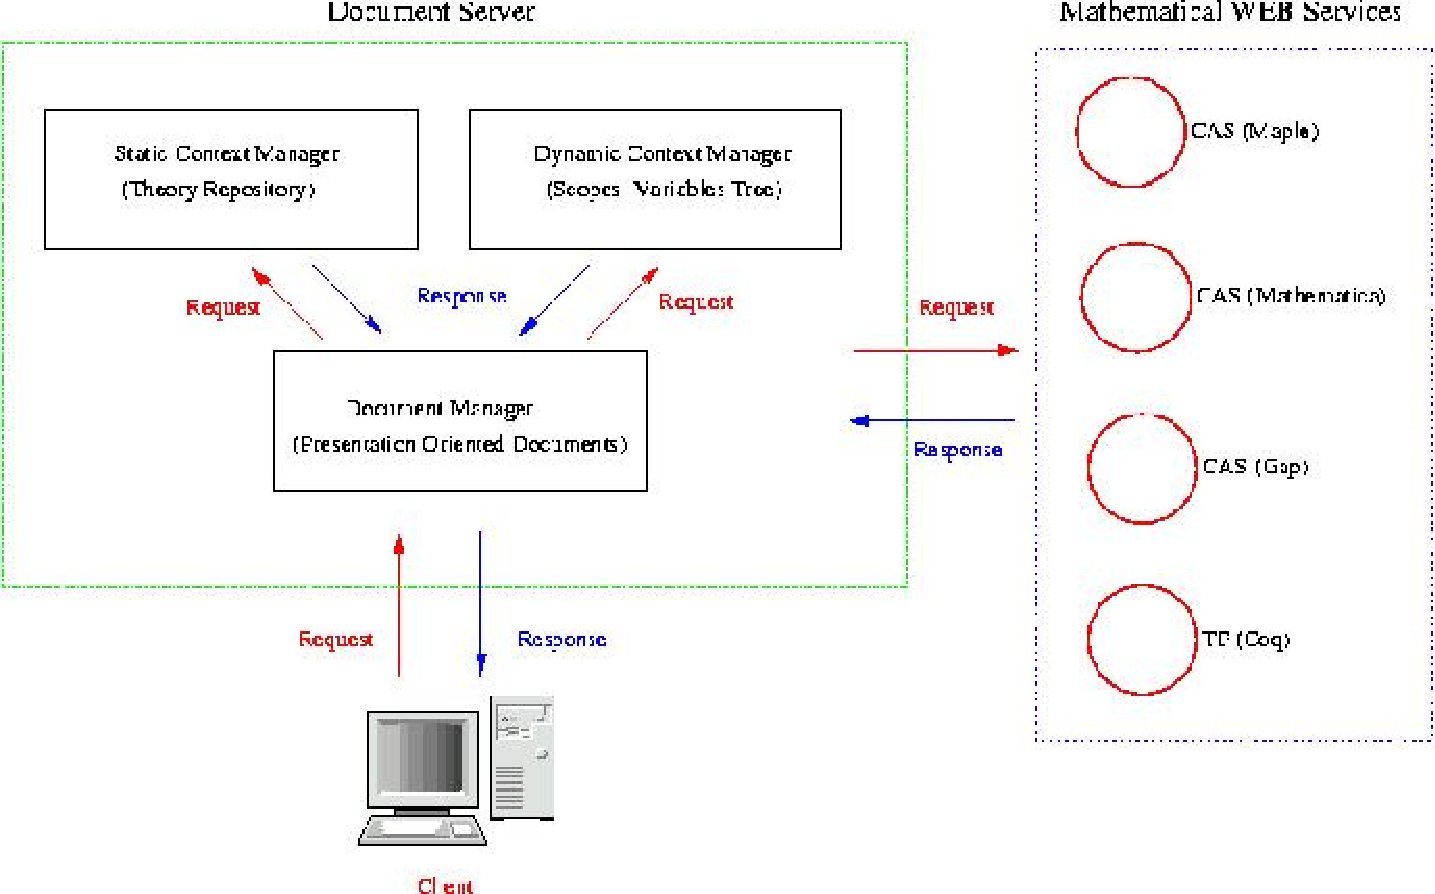
\includegraphics[width=11cm]{projects/mathdox/DocModel}
\end{myfig}

\begin{enumerate}
\item The {\emin{client}}. The client is realized by a
  {\atwintoo{math-enabled}{web}{browser}}.  It will present views of the documents served
  to the user, interact with the user, and communicate user input to the document server.

  The communication between client and server takes place via the HTTP request/response
  mechanism.  The responsibility for interaction is mostly on the server side.
\item The {\twinemph{document}{server}}.  This server caters for presentation,
  communication, and context.  It supports a wide range of actions ranging from handling
  queries to searching within documents for mathematical content and from placing (and
  retrieving) objects into the context, to rendering documents in different views.

  The document server is realized as a Java enhanced
  {\twintoo{web}{application}}~\cite{URL:jsp} inside a web server.  It is not a monolithic
  entity. As shown in {\myfigref{DocModel}}, it is formed by the system parts.  The
  {\twinemph{document}{manager}} serves views to the client.  IMDs can be thought of
  as programs (scripts) encoding the production of a response.  In generating the
  response, they can make use of the information contained in the static context, and in
  the dynamic context (scopes and variables), the user input communicated along with
  request, and the results of computations carried on by one or more mathematical
  services.
  
  Another part is the {\atwinemph{static}{context}{manager}} which is responsible
  for managing a repository of {\MathDox} mathematical theories.
  
  The final (third) part is the {\atwinemph{dynamic}{context}{manager}} which is
  responsible for the dynamic information.

\item {\em\twintoo{mathematical}{service}s}.  Mathematical services can be very diverse:
  some may serve as general interfaces to {\CAS} or to Theorem Provers.  The {\MathDox}
  software provides ways to access these services via standard protocols, among which
  those developed under the MONET project~\cite{URL:monet}.  The mechanism extends the
  phrasebook set-up for {\openmath}~\cite{CapCoh:uosdmc00,CapCoh:jpcaad00}.  For
  constructing specific {\openmath} services, we employ our Java {\openmath} library
  ROML~\cite{URL:roml}.
\end{enumerate}

\subsection{Conclusion}
Now that {\MathDox} is close to a complete working version, trial applications are in the
make. We mention
\begin{itemize}
\item a server for providing designs of experiments on command to statisticians,
\item an exercise repository for the EU funded LeActiveMath project,
\item a mathematics course on calculus, with automated natural language production from a
  formal-mathematical source for the EU funded project WebALT,
\item interactive lecture notes (the successor of~\cite{CohCuySterk:ida99}) for an
  Abstract Algebra course within a mathematically oriented Bachelor curriculum,
\item educational material for highschool mathematics in the Netherlands.
\end{itemize}




%%% Local Variables: 
%%% mode: latex
%%% TeX-master: "../../omdoc"
%%% End: 








% LocalWords:  MathDox mathdox Cuypers Barreiro Eindhoven IMD IMDs CAS DocBook
% LocalWords:  cf phrasebooks Technische Universiteit RIACA Riem Caprotti Sterk
% LocalWords:  Henny Wilbrink Spanbroek Dorina Jibetean DTD HTTP phrasebook ath
% LocalWords:  ROML LeActiveMath WebALT highschool hrasebooks omputer lgebra pp
% LocalWords:  utomated eduction SIGSAM Rom Arjeh ATCM Chiang Chu Jen Chuan eds
% LocalWords:  ISBN Meertens ACELA Kajler Wien JavaServer Franke Ch Sorge vol
% LocalWords:  sk mathdox DocModel mathdox mathdox mathdox mathdox

\end{projectdescription}

\begin{projectdescription}
  %%%%%%%%%%%%%%%%%%%%%%%%%%%%%%%%%%%%%%%%%%%%%%%%%%%%%%%%%%%%%%%%%%%%%%%%%
% This file is part of the LaTeX sources of the OMDoc 1.3 specifiation
% Copyright (c) 2006 Christoph Lange
% This work is licensed by the Creative Commons Share-Alike license
% see http://creativecommons.org/licenses/by-sa/2.5/ for details
\svnInfo $Id: main.tex 8453 2009-08-04 09:58:26Z kohlhase $
\svnKeyword $HeadURL: https://svn.omdoc.org/repos/omdoc/branches/omdoc-1.3/doc/spec/projects/swim/main.tex $
%%%%%%%%%%%%%%%%%%%%%%%%%%%%%%%%%%%%%%%%%%%%%%%%%%%%%%%%%%%%%%%%%%%%%%%%%

\section{{\swim} -- An OMDoc-based Semantic Wiki}
\begin{project}{swim}{http://kwarc.eecs.iu-bremen.de/projects/swim}
\pauthors{Christoph Lange\and Michael Kohlhase}
\pinstitute{Computer Science, International University Bremen}
\end{project}

{\swim} is a semantic wiki for collaboratively building, editing and browsing a
mathematical knowledge base of {\omdoc} theories. Our long-term objective is to develop a
software that facilitates the creation of a shared, public collection of mathematical
knowledge and serves work groups of mathematicians as a tool for collaborative development
of new theories.  Even though the work reported here was initially motivated by solving
the MKM author's dilemma~\cite{KohKoh:cdad04}, we contend that the new application area
MKM can also contribute to the development of semantic wikis.

Technically, {\swim} is based on the semantic wiki engine
\scsys{IkeWiki}~\cite{schaffert06:ikewiki}, which was chosen because of its
modular design, its rich semantic web infrastructure, its user assistance for
annotations, and its orientation towards
learning~\cite{schaffert06:learning-with-semantic-wikis}.

\subsection{Semantic Wikis}

A wiki~\cite{LeuCun01:wikiway} is a web server
application that allows users to browse, create, and edit hyperlinked pages in a web
browser, usually using a simple text syntax.  In contrast to most content management
systems, wiki pages are accessible via an URL containing their title.  A new page can be
created by linking from an existent page to the page to be created.  This link will then
lead to an edit form.  Usually, anyone is allowed to edit pages on a wiki, but access can
be restricted.  Other characteristics of wikis include permanent storage of old page
versions (with facilities to display differences between two versions and to restore a
certain version), notification about recent changes, and full-text search.

Semantic
wikis~\cite{voelkel06:semanticwikistateoftheart,TolPas06:wikis-semantic-hypermedia}
enhance wikis by Semantic Web technologies, such as {\rdf}~\cite{LasSwi:rdf99} or
ontologies.  Usually one page represents one concept from a real-world domain, which has a
type, possibly some metadata, and typed links to other concepts.  For example, a link from
a wiki page about ``Life, the Universe and Everything'' to another page about Douglas
Adams could be typed as ``is author of''.  In terms of {\rdf}, this can be expressed by the
following subject--predicate--object triple,

\[
(\mbox{``Douglas Adams''},\;\mbox{isAuthorOf},\;\mbox{``Life, the Universe and
Everything''})
\]

where the \textit{isAuthorOf} relation would be defined in an ontology.  These links are
usually displayed in a navigation box next to the page contents. Semantic wikis only deal
with wiki text, not with mathematics, though some allow to embed mathematical formulae as
presentational-only {\TeX}.

{\swim} encourages users to collaborate: Non-mathematicians can collaborate in creating a
``Wikipedia of mathematics'' by compiling the knowledge available so far, while scientists
can collaboratively develop new theories.  Users get an immediate reward for many of their
contributions: Once they specify the type of a page or relations of one page to another,
this information will be displayed in a box of navigation links.  We intend to make the
data created in {\swim} usable for external services by offering an export facility for
{\omdoc} documents and by integrating them into {\swim}.  Mathematicians developing
theories will be assisted to retain an overview of theory dependencies in order not to
break them.  Social software services will further utilize the semantic information
available from the theories and from tracking the user interaction log (``Who did what on
which page when?'').  User feedback to pages can be extended to social bookmarking, which
is ``the practice of saving bookmarks [of Internet resources] to a public web site and
`tagging' them with keywords.''~\cite{lomas05:social-bookmarking} The more users tag a
certain resource, the higher a social bookmarking service will rank it.

The enhancements of the data model semantic wikis bring along --- compared to traditional
wikis --- are already present in the {\omdoc} format, so that an {\omdoc}-based wiki only
needs to operationalize their underlying meaning. For example, typed links, which are
implemented via an extension to the wiki syntax in \scsys{Semantic
  MediaWiki}~\cite{voelkel06:semanticwikipedia} or editable through a separate editor in
\scsys{IkeWiki}~\cite{schaffert06:ikewiki}, are implemented by means of the \texttt{for}
attribute to {\omdoc}'s elements (e.g.\ \texttt{<example for="\#id-of-assertion">}).
{\swim} makes them editable easily and visualizes them adequately.  A semantic wiki
targeted at mathematics must ensure that dependencies between concepts are preserved.
Results in this area will be interesting for non-mathematical semantic wikis as well,
especially when they support higher levels of formalization such as ontologies.

\subsection{Design of {\swim}}

\subsubsection{Concepts and Relations}

The smallest unit that can be displayed, edited, linked to, or archived in a wiki is a
page. In a semantic wiki, it usually describes one {\emph{concept}}, including its
properties and its relations to other concepts.  While standalone {\omdoc} documents can
contain more than one theory, is is important to keep pages small in a wiki to improve the
effectivity of usage.  Furthermore, usual semantic wikis only store and display metadata
and typed links per page; {\swim} does too.\footnote{Semantic information will only be
  considered on the theory and statement levels of {\omdoc} --- directly or through
  reasoning in the case of transitive closures ---, not on the object level.}  Users are
strongly encouraged to define at most one theory per wiki page and to roll out
non-constitutive statements (see {\mysecref{statements-constitutive}}) to separate pages,
referencing their context theory.  As constitutive statements cannot exist without an
enclosing theory, but as, on the other hand, we want each wiki page to form a valid
document, we introduced a new element {\element[ns-elt=swim]{page}}, which can be a child
of an {\element{omdoc}} element and which has the same content model as a
{\element{theory}} element --- in particular, it can hold several theory-constitutive
statements and connect them to their context theory.
\begin{wrapfigure}{r}{8cm}
  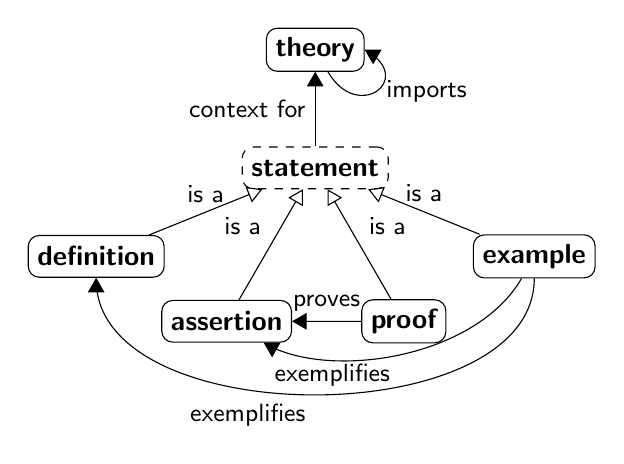
\begin{tikzpicture}[scale=1.5,thin,font=\sffamily,>=triangle 60]
    \tikzstyle{concept}=[font=\sffamily\bfseries,draw,minimum height=3.5ex,rounded corners]
    \tikzstyle{every path}=[font=\small\sffamily];
    \node[concept] (t) at (0,1) {theory};
    \node[concept,dashed] (s) at (0,0) {\itshape statement};
    \node[concept] (d) at +(-158:2.0cm) {definition};
    \begin{scope}[shift={(d)}]% control point for e->d
      \coordinate (da) at +(-90:1.5cm);% relative to s, not to a!
    \end{scope}
    \node[concept] (a) at +(-120:1.5cm) {assertion};
    \begin{scope}[shift={(a)}]% control point for e->a
      \coordinate (aa) at +(-30:1cm);% relative to s, not to a!
    \end{scope}
    \node[concept] (p) at +(-60:1.5cm) {proof};
    \node[concept] (e) at +(-22:2.0cm) {example};
    \draw[->] (t.-60) .. controls +(-60:0.5cm) and +(-30:0.5cm) .. node[right]
    {imports} (t.east);
    \draw[->] (s) -- node[left] {context for} (t);
    \draw[-open triangle 60] (d) -- node[above] {is a} (s);
    \draw[-open triangle 60] (a) -- node[above left] {is a} (s);
    \draw[-open triangle 60] (p) -- node[above right] {is a} (s);
    \draw[-open triangle 60] (e) -- node[above] {is a} (s);
    \draw[->] (p) -- node[above] {proves} (a);
    \draw[->] (e) ..
    controls +(-120:1cm)
    and (aa) ..
    node[below left] {exemplifies} (a);
    \draw[->] (e) ..
    controls +(-90:1.5cm)
    and (da) ..
    node[below left] {exemplifies} (d);
  \end{tikzpicture}
  \caption{Subset of {\omdoc}'s system ontology}\vspace*{-.5cm}
\end{wrapfigure}
{\omdoc}'s system ontology has been partly coded in OWL-DL and imported to the wiki's {\rdf}
store, which is implemented using the Jena Semantic Web Framework for
Java~\cite{URL:jena:web}. Theories as well as statements of any type form concepts, and
the most important relations between those concepts are extracted from the {\omdoc} pages
on saving and then stored as {\rdf} triples.  These relations include:
\begin{itemize}
\item The import relation between theories
\item The relation of a statement to its context theory
\item The relation of an example to the statement it exemplifies
\item The relation of a proof to the assertion it proves
\end{itemize}
It is planned to also take relations given by user interaction into consideration, such as
``Who edited which page when?'', and to combine ontology-defined relations and user
relations.  For example, a metric estimating the {\emph{degree of difficulty}} of a page,
calculated by counting the questions on the discussion page, could be implemented.
Furthermore, the user can specify taxonomic relations, which cannot be stated explicitly
in {\omdoc}, such as (``all differentiable functions are continuous''), as annotations in
an ontology language like {\rdf} Schema or {\owl}.

\subsubsection{User Interface and Interaction Model}

Pages can be rendered to XHTML plus presentational MathML using the transformations
described in {\mychapref{transform-xsl}}. There is also a browsable source code view, which is
useful for documents that are not written in textbook style.

Not only will the user be able to navigate along the dependency graph, she will also be
able to {\emph{interact}} with the system: she will be asked whether she wants to explore
the theories required as dependencies in further detail.

Suppose that the user is currently reading the page containing the theory {\snippet{ring}}
from the elementary algebra example from {\mychapref{dg-elal}}. In this case the wiki will
not only display navigation links to the direct dependencies {\snippet{group}} and
{\snippet{monoid}}, but it will also provide unobtrusive buttons that allow the user to
give one of the commands in {\myfigref{gui-showdeps}}. Not only the last case will be
recorded --- the others are interesting as well for \emph{social bookmarking}.  For
example, if many users requested a theory $t$ to be explained, the system could default to
display not only the direct dependencies but also the level-two dependencies, for it seems
that $t$ is too difficult for only being explained shallowly.

\begin{myfig}{gui-showdeps}{The command buttons to navigate along the dependencies}
  \begin{minipage}{8cm}
\begin{description}
\item[{\bf{No, thanks!}}] ``{\emph{I already know group and monoid.}}''
\item[{\bf{Explain}}] ``{\emph{Please show me group and monoid, I want to learn about
      ring's prerequisites.}}'' --- group and monoid will be displayed.
\item[{\bf{Explore}}] ``{\emph{Please show me {\emph{all}} prerequisites for ring.}}'' ---
  group, monoid, and semigroup, are opened in separate windows or serialized into one
  page.
\item[{\bf{Suspend}}] ``{\emph{I want to know about group and monoid, but only later.}}''
  --- {\swim} keeps a notice in the user's profile that she wants to read group and monoid
  sometime.  Reminder links to suspended theories are shown on a separate navigation bar.
\end{description}
\end{minipage}\quad
\begin{minipage}{2.5cm}
  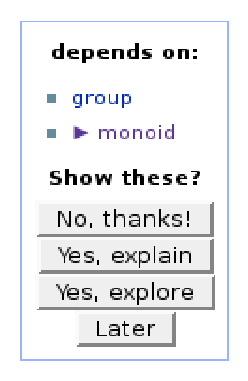
\includegraphics[width=2.5cm]{projects/swim/gui-showdeps}
\end{minipage}
\end{myfig}

\subsubsection{Further work}

Further work on {\swim} will concentrate on integrating a lightweight
management of change process.  Second, while the wiki is yet a user-friendly
\emph{browser}, there is still a demand for assisting users to \emph{edit}
{\omdoc}.  To this end, the {\qmath} preprocessor (see {\mysecref{qmath}}) will
be integrated into {\swim}.  Mathematical objects entered as {\qmath} will be
kept in this syntax for display in the edit form, but they will be converted to
{\omdoc} for rendering for presentation and when pages are exported to another
application.

%%% Local Variables: 
%%% mode: stex
%%% TeX-master: "../../omdoc"
%%% End: 

% LocalWords:  matwebsearch Ioan Sucan nC dx dy dt runningex XPointer ns attr
% LocalWords:  mq anyorder xmlns domainofapplication bvar ci cn eq OAI API da
% LocalWords:  Lange CPoint wikis dateness parseable isAuthorOf MediaWiki omdoc
% LocalWords:  aa wiki's Wiki wiki IkeWiki JA hypermedia elt semithick pres dg
% LocalWords:  elal gui showdeps qmath stex metadata wiki's scheint mir kein zu
% LocalWords:  Gegensatz sein

\end{projectdescription}

\begin{projectdescription}
  %%%%%%%%%%%%%%%%%%%%%%%%%%%%%%%%%%%%%%%%%%%%%%%%%%%%%%%%%%%%%%%%%%%%%%%%%
% This file is part of the LaTeX sources of the OMDoc 1.3 specifiation
% Copyright (c) 2006 Paul Libbrecht
% This work is licensed by the Creative Commons Share-Alike license
% see http://creativecommons.org/licenses/by-sa/2.5/ for details
\svnInfo $Id: authoring.tex 8453 2009-08-04 09:58:26Z kohlhase $
\svnKeyword $HeadURL: https://svn.omdoc.org/repos/omdoc/branches/omdoc-1.3/doc/spec/projects/activemath/authoring.tex $
%%%%%%%%%%%%%%%%%%%%%%%%%%%%%%%%%%%%%%%%%%%%%%%%%%%%%%%%%%%%%%%%%%%%%%%%%

\section{Authoring Tools for {\activemath}}
\begin{project}{jeditoqmath}{http://www.activemath.org/projects/jEditOQMath}
  \pauthors{Paul Libbrecht} 
  \pinstitute{DFKI GmbH and Universit{\"a}t des Saarlandes}
\end{project}


The {\omdoc} content to be delivered by {\activemath} are {\omdoc} documents with
{\openmath} formulae. Experience has shown that writing the {\xml}-source by hand is
feasible and even preferred if the author wants to follow the evolution of content's
structure.  It is similar to {\html} editing.  However, the complexity of {\xml} makes it
hard to keep an overview when writing mathematical expressions. Therefore, the
{\scsys{OQMath}} processor has been implemented: it uses {\scsys{QMath}} for formulae and
leaves the rest of the {\omdoc} written as usual {\xml}.

{\scsys{OQMath}} has been integrated in a supporting {\xml}-editor, jEdit. This editor
provides structural support at writing {\xml}-documents. Authors, even with no
{\xml}-knowledge, can easily write valid document {\scsys{jEditOQMath}}.  This package
includes, in a one-click installer, {\qmath}, {\scsys{OQMath}}, {\scsys{jEdit}}, and
Ant-scripts for publication of the content in {\activemath} knowledge bases.  These
scripts validate the references in the content.  These scripts also provide authors with
short cycles edit-in-{\scsys{jEditOQMath}}-and-test-in-{\activemath}.  More about
{\scsys{jEditOQMath}} can be seen from
{\url{http://www.activemath.org/projects/jEditOQMath}} at~\cite{AM-authoring-from-dev-on}

%Explorations of knowledge navigation and edition using the Protege%
%\footnote{See \url{http://protege.semanticweb.org/}.}
%ontology editor
%have been made but limitations of the visualization library have plagued this first visual
%editor attempts.

%Access to the other {\omdoc} content in order for them to be referenced, used, or inspected
%has turned out to be an essential requirement of authoring tools: 
{\scsys{jEditOQMath}} provides search facilities as well as contextual drops from items
presented in an {\activemath} window.  This way the testing of content in the target
environment and the authoring experience are bound tighter together,
% binds even tighter the test-running of content in the environment where it will be
%delivered to the authoring experience, 
thus making {\scsys{jEditOQMath}} closer to the WYSIWYG paradigm without being limited to
its simple visual incarnation.

%exercise authoring tool for 'authoring by demonstration'
%---- Ian or George here ----
% George: I can not write anything yet, there is no version of a tool releazed

% abundant  experience with authors
To date, more than $10'000$ {\emph{items}} of {\omdoc} content has been written using
these authoring tools in Algebra and Calculus. This experience with authors considerably
improved our understanding of what today's authors need and what different classes of
authors can cope with.

% has allowed us to
% gear features of the authoring tools towards users and has shown gaps still to be filled.

Among the greatest difficulties of authoring content for {\activemath} was the art of
properly choosing mathematical semantic encoding: the mathematical discourse is made of
very fine notation rules along with subtle digressions to these rules...  formalizing
them, as is needed when writing {\openmath} or the {\qmath} formulae for them, turns out
to often be overwhelming.  The usage of the ellipsis in such a formula as $1, \dots, k,
\dots, n$ is a simple example of semantic encoding challenge. The knowledge organization
of {\omdoc} that makes it possible to define one's own {\openmath} symbols has been a key
ingredient to facing this challenge.

Among the features most requested by authors, which we have tried to answer 
as much as possible,  are a short edit-and-test cycle and validation facilities 
taking in account the overall content.

\subsubsection{Validation Tools}

Automated validation of {\omdoc} content has many facets.
% can be done in many respects but little has been done with {\omdoc} documents.
{\xml}-validation with a DTD and Schema is a first step.  However there are still many
structure rules mentioned only as human readable forms in the {\omdoc} specifications.
References between {\omdoc} items is another important facet which has been answered by
{\activemath} knowledge bases and publishing scripts.  Experience has proved that ignoring
such errors has lead repeatedly to authors complaining about the weirdest behaviours of
the overall learning environment.  Many other simple validations could be done in order to
support the author, for example the validation of a picture embedding, or of fine grained
typing of relations (for example, that a definition should only be {\emph{for}} a symbol).

Further validation tools are being investigated, for example, those tuned to particular
pedagogical scenarios.


\subsubsection{Further Authoring Tools for {\activemath}} {\scsys{jEditOQMath}} clearly
remains for users who feel comfortable with source editing. Experience has shown that
authors having written {\html} or {\TeX} earlier did not find this paradigm problematic.
It is, however, a steep learning slope for beginner authors.  A more visual component is
being worked upon, able to display and edit visually the children of a \element{CMP},
including formulae.\footnote{More about the component for {\omdoc} micro-structure can be
  read from \url{http://www.activemath.org/projects/OmdocJdomAuthoring/}.}  This
component, along with forms and summaries for metadata, should provide a visual
environment to edit {\omdoc} content for {\activemath} in a relatively accessible way.

Another area where source editing has shown difficulties is in the process of authoring
exercises with many steps... the rich structure of the exercises, along with the non-neglect able
space taken by the display of {\xml}-source has challenged several authors, having
difficulties to overview such sources as 600 Kb of {\scsys{OQMath}} source for a single
exercise. 
A web-based visual authoring environment is under work within the {\activemath} group.

%%% Local Variables: 
%%% mode: stex
%%% TeX-master: "../../omdoc"
%%% End: 

% LocalWords:  jeditoqmath Libbrecht GmbH Universit des Saarlandes OQMath QMath
% LocalWords:  jEdit jEditOQMath jEditOQMath jEditOQMath jEditOQMath one's
% LocalWords:  jEditOQMath jEditOQMath jEditOQMath jEditOQMath jEditOQMath
% LocalWords:  jEditOQMath jEditOQMath jEditOQMath metadata jEditOQMath
% LocalWords:  jEditOQMath jEditOQMath jEditOQMath jEditOQMath jEditOQMath

\end{projectdescription}

\begin{projectdescription}
  %%%%%%%%%%%%%%%%%%%%%%%%%%%%%%%%%%%%%%%%%%%%%%%%%%%%%%%%%%%%%%%%%%%%%%%%%
% This file is part of the LaTeX sources of the OMDoc 1.3 specifiation
% Copyright (c) 2006 Christoph Lange
% This work is licensed by the Creative Commons Share-Alike license
% see http://creativecommons.org/licenses/by-sa/2.5/ for details
\svnInfo $Id: main.tex 8453 2009-08-04 09:58:26Z kohlhase $
\svnKeyword $HeadURL: https://svn.omdoc.org/repos/omdoc/branches/omdoc-1.3/doc/spec/projects/swim/main.tex $
%%%%%%%%%%%%%%%%%%%%%%%%%%%%%%%%%%%%%%%%%%%%%%%%%%%%%%%%%%%%%%%%%%%%%%%%%

\section{{\swim} -- An OMDoc-based Semantic Wiki}
\begin{project}{swim}{http://kwarc.eecs.iu-bremen.de/projects/swim}
\pauthors{Christoph Lange\and Michael Kohlhase}
\pinstitute{Computer Science, International University Bremen}
\end{project}

{\swim} is a semantic wiki for collaboratively building, editing and browsing a
mathematical knowledge base of {\omdoc} theories. Our long-term objective is to develop a
software that facilitates the creation of a shared, public collection of mathematical
knowledge and serves work groups of mathematicians as a tool for collaborative development
of new theories.  Even though the work reported here was initially motivated by solving
the MKM author's dilemma~\cite{KohKoh:cdad04}, we contend that the new application area
MKM can also contribute to the development of semantic wikis.

Technically, {\swim} is based on the semantic wiki engine
\scsys{IkeWiki}~\cite{schaffert06:ikewiki}, which was chosen because of its
modular design, its rich semantic web infrastructure, its user assistance for
annotations, and its orientation towards
learning~\cite{schaffert06:learning-with-semantic-wikis}.

\subsection{Semantic Wikis}

A wiki~\cite{LeuCun01:wikiway} is a web server
application that allows users to browse, create, and edit hyperlinked pages in a web
browser, usually using a simple text syntax.  In contrast to most content management
systems, wiki pages are accessible via an URL containing their title.  A new page can be
created by linking from an existent page to the page to be created.  This link will then
lead to an edit form.  Usually, anyone is allowed to edit pages on a wiki, but access can
be restricted.  Other characteristics of wikis include permanent storage of old page
versions (with facilities to display differences between two versions and to restore a
certain version), notification about recent changes, and full-text search.

Semantic
wikis~\cite{voelkel06:semanticwikistateoftheart,TolPas06:wikis-semantic-hypermedia}
enhance wikis by Semantic Web technologies, such as {\rdf}~\cite{LasSwi:rdf99} or
ontologies.  Usually one page represents one concept from a real-world domain, which has a
type, possibly some metadata, and typed links to other concepts.  For example, a link from
a wiki page about ``Life, the Universe and Everything'' to another page about Douglas
Adams could be typed as ``is author of''.  In terms of {\rdf}, this can be expressed by the
following subject--predicate--object triple,

\[
(\mbox{``Douglas Adams''},\;\mbox{isAuthorOf},\;\mbox{``Life, the Universe and
Everything''})
\]

where the \textit{isAuthorOf} relation would be defined in an ontology.  These links are
usually displayed in a navigation box next to the page contents. Semantic wikis only deal
with wiki text, not with mathematics, though some allow to embed mathematical formulae as
presentational-only {\TeX}.

{\swim} encourages users to collaborate: Non-mathematicians can collaborate in creating a
``Wikipedia of mathematics'' by compiling the knowledge available so far, while scientists
can collaboratively develop new theories.  Users get an immediate reward for many of their
contributions: Once they specify the type of a page or relations of one page to another,
this information will be displayed in a box of navigation links.  We intend to make the
data created in {\swim} usable for external services by offering an export facility for
{\omdoc} documents and by integrating them into {\swim}.  Mathematicians developing
theories will be assisted to retain an overview of theory dependencies in order not to
break them.  Social software services will further utilize the semantic information
available from the theories and from tracking the user interaction log (``Who did what on
which page when?'').  User feedback to pages can be extended to social bookmarking, which
is ``the practice of saving bookmarks [of Internet resources] to a public web site and
`tagging' them with keywords.''~\cite{lomas05:social-bookmarking} The more users tag a
certain resource, the higher a social bookmarking service will rank it.

The enhancements of the data model semantic wikis bring along --- compared to traditional
wikis --- are already present in the {\omdoc} format, so that an {\omdoc}-based wiki only
needs to operationalize their underlying meaning. For example, typed links, which are
implemented via an extension to the wiki syntax in \scsys{Semantic
  MediaWiki}~\cite{voelkel06:semanticwikipedia} or editable through a separate editor in
\scsys{IkeWiki}~\cite{schaffert06:ikewiki}, are implemented by means of the \texttt{for}
attribute to {\omdoc}'s elements (e.g.\ \texttt{<example for="\#id-of-assertion">}).
{\swim} makes them editable easily and visualizes them adequately.  A semantic wiki
targeted at mathematics must ensure that dependencies between concepts are preserved.
Results in this area will be interesting for non-mathematical semantic wikis as well,
especially when they support higher levels of formalization such as ontologies.

\subsection{Design of {\swim}}

\subsubsection{Concepts and Relations}

The smallest unit that can be displayed, edited, linked to, or archived in a wiki is a
page. In a semantic wiki, it usually describes one {\emph{concept}}, including its
properties and its relations to other concepts.  While standalone {\omdoc} documents can
contain more than one theory, is is important to keep pages small in a wiki to improve the
effectivity of usage.  Furthermore, usual semantic wikis only store and display metadata
and typed links per page; {\swim} does too.\footnote{Semantic information will only be
  considered on the theory and statement levels of {\omdoc} --- directly or through
  reasoning in the case of transitive closures ---, not on the object level.}  Users are
strongly encouraged to define at most one theory per wiki page and to roll out
non-constitutive statements (see {\mysecref{statements-constitutive}}) to separate pages,
referencing their context theory.  As constitutive statements cannot exist without an
enclosing theory, but as, on the other hand, we want each wiki page to form a valid
document, we introduced a new element {\element[ns-elt=swim]{page}}, which can be a child
of an {\element{omdoc}} element and which has the same content model as a
{\element{theory}} element --- in particular, it can hold several theory-constitutive
statements and connect them to their context theory.
\begin{wrapfigure}{r}{8cm}
  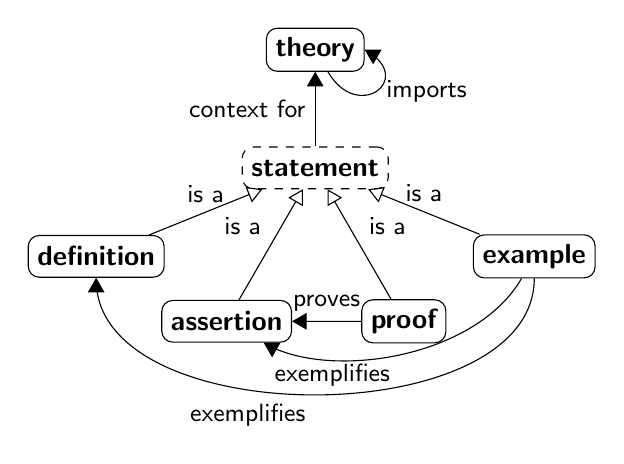
\begin{tikzpicture}[scale=1.5,thin,font=\sffamily,>=triangle 60]
    \tikzstyle{concept}=[font=\sffamily\bfseries,draw,minimum height=3.5ex,rounded corners]
    \tikzstyle{every path}=[font=\small\sffamily];
    \node[concept] (t) at (0,1) {theory};
    \node[concept,dashed] (s) at (0,0) {\itshape statement};
    \node[concept] (d) at +(-158:2.0cm) {definition};
    \begin{scope}[shift={(d)}]% control point for e->d
      \coordinate (da) at +(-90:1.5cm);% relative to s, not to a!
    \end{scope}
    \node[concept] (a) at +(-120:1.5cm) {assertion};
    \begin{scope}[shift={(a)}]% control point for e->a
      \coordinate (aa) at +(-30:1cm);% relative to s, not to a!
    \end{scope}
    \node[concept] (p) at +(-60:1.5cm) {proof};
    \node[concept] (e) at +(-22:2.0cm) {example};
    \draw[->] (t.-60) .. controls +(-60:0.5cm) and +(-30:0.5cm) .. node[right]
    {imports} (t.east);
    \draw[->] (s) -- node[left] {context for} (t);
    \draw[-open triangle 60] (d) -- node[above] {is a} (s);
    \draw[-open triangle 60] (a) -- node[above left] {is a} (s);
    \draw[-open triangle 60] (p) -- node[above right] {is a} (s);
    \draw[-open triangle 60] (e) -- node[above] {is a} (s);
    \draw[->] (p) -- node[above] {proves} (a);
    \draw[->] (e) ..
    controls +(-120:1cm)
    and (aa) ..
    node[below left] {exemplifies} (a);
    \draw[->] (e) ..
    controls +(-90:1.5cm)
    and (da) ..
    node[below left] {exemplifies} (d);
  \end{tikzpicture}
  \caption{Subset of {\omdoc}'s system ontology}\vspace*{-.5cm}
\end{wrapfigure}
{\omdoc}'s system ontology has been partly coded in OWL-DL and imported to the wiki's {\rdf}
store, which is implemented using the Jena Semantic Web Framework for
Java~\cite{URL:jena:web}. Theories as well as statements of any type form concepts, and
the most important relations between those concepts are extracted from the {\omdoc} pages
on saving and then stored as {\rdf} triples.  These relations include:
\begin{itemize}
\item The import relation between theories
\item The relation of a statement to its context theory
\item The relation of an example to the statement it exemplifies
\item The relation of a proof to the assertion it proves
\end{itemize}
It is planned to also take relations given by user interaction into consideration, such as
``Who edited which page when?'', and to combine ontology-defined relations and user
relations.  For example, a metric estimating the {\emph{degree of difficulty}} of a page,
calculated by counting the questions on the discussion page, could be implemented.
Furthermore, the user can specify taxonomic relations, which cannot be stated explicitly
in {\omdoc}, such as (``all differentiable functions are continuous''), as annotations in
an ontology language like {\rdf} Schema or {\owl}.

\subsubsection{User Interface and Interaction Model}

Pages can be rendered to XHTML plus presentational MathML using the transformations
described in {\mychapref{transform-xsl}}. There is also a browsable source code view, which is
useful for documents that are not written in textbook style.

Not only will the user be able to navigate along the dependency graph, she will also be
able to {\emph{interact}} with the system: she will be asked whether she wants to explore
the theories required as dependencies in further detail.

Suppose that the user is currently reading the page containing the theory {\snippet{ring}}
from the elementary algebra example from {\mychapref{dg-elal}}. In this case the wiki will
not only display navigation links to the direct dependencies {\snippet{group}} and
{\snippet{monoid}}, but it will also provide unobtrusive buttons that allow the user to
give one of the commands in {\myfigref{gui-showdeps}}. Not only the last case will be
recorded --- the others are interesting as well for \emph{social bookmarking}.  For
example, if many users requested a theory $t$ to be explained, the system could default to
display not only the direct dependencies but also the level-two dependencies, for it seems
that $t$ is too difficult for only being explained shallowly.

\begin{myfig}{gui-showdeps}{The command buttons to navigate along the dependencies}
  \begin{minipage}{8cm}
\begin{description}
\item[{\bf{No, thanks!}}] ``{\emph{I already know group and monoid.}}''
\item[{\bf{Explain}}] ``{\emph{Please show me group and monoid, I want to learn about
      ring's prerequisites.}}'' --- group and monoid will be displayed.
\item[{\bf{Explore}}] ``{\emph{Please show me {\emph{all}} prerequisites for ring.}}'' ---
  group, monoid, and semigroup, are opened in separate windows or serialized into one
  page.
\item[{\bf{Suspend}}] ``{\emph{I want to know about group and monoid, but only later.}}''
  --- {\swim} keeps a notice in the user's profile that she wants to read group and monoid
  sometime.  Reminder links to suspended theories are shown on a separate navigation bar.
\end{description}
\end{minipage}\quad
\begin{minipage}{2.5cm}
  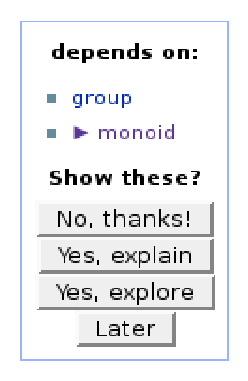
\includegraphics[width=2.5cm]{projects/swim/gui-showdeps}
\end{minipage}
\end{myfig}

\subsubsection{Further work}

Further work on {\swim} will concentrate on integrating a lightweight
management of change process.  Second, while the wiki is yet a user-friendly
\emph{browser}, there is still a demand for assisting users to \emph{edit}
{\omdoc}.  To this end, the {\qmath} preprocessor (see {\mysecref{qmath}}) will
be integrated into {\swim}.  Mathematical objects entered as {\qmath} will be
kept in this syntax for display in the edit form, but they will be converted to
{\omdoc} for rendering for presentation and when pages are exported to another
application.

%%% Local Variables: 
%%% mode: stex
%%% TeX-master: "../../omdoc"
%%% End: 

% LocalWords:  matwebsearch Ioan Sucan nC dx dy dt runningex XPointer ns attr
% LocalWords:  mq anyorder xmlns domainofapplication bvar ci cn eq OAI API da
% LocalWords:  Lange CPoint wikis dateness parseable isAuthorOf MediaWiki omdoc
% LocalWords:  aa wiki's Wiki wiki IkeWiki JA hypermedia elt semithick pres dg
% LocalWords:  elal gui showdeps qmath stex metadata wiki's scheint mir kein zu
% LocalWords:  Gegensatz sein

\end{projectdescription}

\begin{projectdescription}
  %%%%%%%%%%%%%%%%%%%%%%%%%%%%%%%%%%%%%%%%%%%%%%%%%%%%%%%%%%%%%%%%%%%%%%%%%
% This file is part of the LaTeX sources of the OMDoc 1.3 specifiation
% Copyright (c) 2006 Christoph Lange
% This work is licensed by the Creative Commons Share-Alike license
% see http://creativecommons.org/licenses/by-sa/2.5/ for details
\svnInfo $Id: main.tex 8453 2009-08-04 09:58:26Z kohlhase $
\svnKeyword $HeadURL: https://svn.omdoc.org/repos/omdoc/branches/omdoc-1.3/doc/spec/projects/swim/main.tex $
%%%%%%%%%%%%%%%%%%%%%%%%%%%%%%%%%%%%%%%%%%%%%%%%%%%%%%%%%%%%%%%%%%%%%%%%%

\section{{\swim} -- An OMDoc-based Semantic Wiki}
\begin{project}{swim}{http://kwarc.eecs.iu-bremen.de/projects/swim}
\pauthors{Christoph Lange\and Michael Kohlhase}
\pinstitute{Computer Science, International University Bremen}
\end{project}

{\swim} is a semantic wiki for collaboratively building, editing and browsing a
mathematical knowledge base of {\omdoc} theories. Our long-term objective is to develop a
software that facilitates the creation of a shared, public collection of mathematical
knowledge and serves work groups of mathematicians as a tool for collaborative development
of new theories.  Even though the work reported here was initially motivated by solving
the MKM author's dilemma~\cite{KohKoh:cdad04}, we contend that the new application area
MKM can also contribute to the development of semantic wikis.

Technically, {\swim} is based on the semantic wiki engine
\scsys{IkeWiki}~\cite{schaffert06:ikewiki}, which was chosen because of its
modular design, its rich semantic web infrastructure, its user assistance for
annotations, and its orientation towards
learning~\cite{schaffert06:learning-with-semantic-wikis}.

\subsection{Semantic Wikis}

A wiki~\cite{LeuCun01:wikiway} is a web server
application that allows users to browse, create, and edit hyperlinked pages in a web
browser, usually using a simple text syntax.  In contrast to most content management
systems, wiki pages are accessible via an URL containing their title.  A new page can be
created by linking from an existent page to the page to be created.  This link will then
lead to an edit form.  Usually, anyone is allowed to edit pages on a wiki, but access can
be restricted.  Other characteristics of wikis include permanent storage of old page
versions (with facilities to display differences between two versions and to restore a
certain version), notification about recent changes, and full-text search.

Semantic
wikis~\cite{voelkel06:semanticwikistateoftheart,TolPas06:wikis-semantic-hypermedia}
enhance wikis by Semantic Web technologies, such as {\rdf}~\cite{LasSwi:rdf99} or
ontologies.  Usually one page represents one concept from a real-world domain, which has a
type, possibly some metadata, and typed links to other concepts.  For example, a link from
a wiki page about ``Life, the Universe and Everything'' to another page about Douglas
Adams could be typed as ``is author of''.  In terms of {\rdf}, this can be expressed by the
following subject--predicate--object triple,

\[
(\mbox{``Douglas Adams''},\;\mbox{isAuthorOf},\;\mbox{``Life, the Universe and
Everything''})
\]

where the \textit{isAuthorOf} relation would be defined in an ontology.  These links are
usually displayed in a navigation box next to the page contents. Semantic wikis only deal
with wiki text, not with mathematics, though some allow to embed mathematical formulae as
presentational-only {\TeX}.

{\swim} encourages users to collaborate: Non-mathematicians can collaborate in creating a
``Wikipedia of mathematics'' by compiling the knowledge available so far, while scientists
can collaboratively develop new theories.  Users get an immediate reward for many of their
contributions: Once they specify the type of a page or relations of one page to another,
this information will be displayed in a box of navigation links.  We intend to make the
data created in {\swim} usable for external services by offering an export facility for
{\omdoc} documents and by integrating them into {\swim}.  Mathematicians developing
theories will be assisted to retain an overview of theory dependencies in order not to
break them.  Social software services will further utilize the semantic information
available from the theories and from tracking the user interaction log (``Who did what on
which page when?'').  User feedback to pages can be extended to social bookmarking, which
is ``the practice of saving bookmarks [of Internet resources] to a public web site and
`tagging' them with keywords.''~\cite{lomas05:social-bookmarking} The more users tag a
certain resource, the higher a social bookmarking service will rank it.

The enhancements of the data model semantic wikis bring along --- compared to traditional
wikis --- are already present in the {\omdoc} format, so that an {\omdoc}-based wiki only
needs to operationalize their underlying meaning. For example, typed links, which are
implemented via an extension to the wiki syntax in \scsys{Semantic
  MediaWiki}~\cite{voelkel06:semanticwikipedia} or editable through a separate editor in
\scsys{IkeWiki}~\cite{schaffert06:ikewiki}, are implemented by means of the \texttt{for}
attribute to {\omdoc}'s elements (e.g.\ \texttt{<example for="\#id-of-assertion">}).
{\swim} makes them editable easily and visualizes them adequately.  A semantic wiki
targeted at mathematics must ensure that dependencies between concepts are preserved.
Results in this area will be interesting for non-mathematical semantic wikis as well,
especially when they support higher levels of formalization such as ontologies.

\subsection{Design of {\swim}}

\subsubsection{Concepts and Relations}

The smallest unit that can be displayed, edited, linked to, or archived in a wiki is a
page. In a semantic wiki, it usually describes one {\emph{concept}}, including its
properties and its relations to other concepts.  While standalone {\omdoc} documents can
contain more than one theory, is is important to keep pages small in a wiki to improve the
effectivity of usage.  Furthermore, usual semantic wikis only store and display metadata
and typed links per page; {\swim} does too.\footnote{Semantic information will only be
  considered on the theory and statement levels of {\omdoc} --- directly or through
  reasoning in the case of transitive closures ---, not on the object level.}  Users are
strongly encouraged to define at most one theory per wiki page and to roll out
non-constitutive statements (see {\mysecref{statements-constitutive}}) to separate pages,
referencing their context theory.  As constitutive statements cannot exist without an
enclosing theory, but as, on the other hand, we want each wiki page to form a valid
document, we introduced a new element {\element[ns-elt=swim]{page}}, which can be a child
of an {\element{omdoc}} element and which has the same content model as a
{\element{theory}} element --- in particular, it can hold several theory-constitutive
statements and connect them to their context theory.
\begin{wrapfigure}{r}{8cm}
  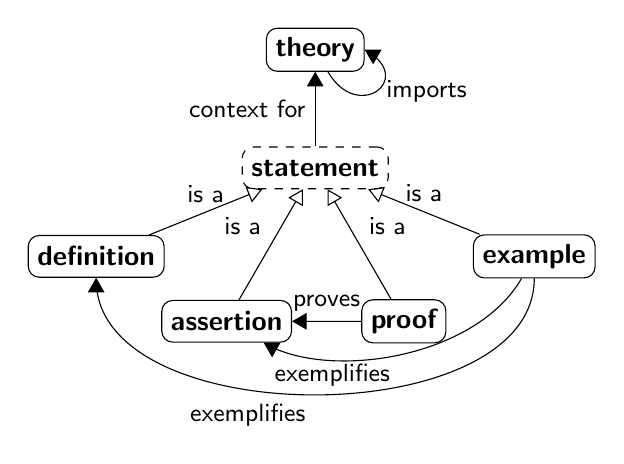
\begin{tikzpicture}[scale=1.5,thin,font=\sffamily,>=triangle 60]
    \tikzstyle{concept}=[font=\sffamily\bfseries,draw,minimum height=3.5ex,rounded corners]
    \tikzstyle{every path}=[font=\small\sffamily];
    \node[concept] (t) at (0,1) {theory};
    \node[concept,dashed] (s) at (0,0) {\itshape statement};
    \node[concept] (d) at +(-158:2.0cm) {definition};
    \begin{scope}[shift={(d)}]% control point for e->d
      \coordinate (da) at +(-90:1.5cm);% relative to s, not to a!
    \end{scope}
    \node[concept] (a) at +(-120:1.5cm) {assertion};
    \begin{scope}[shift={(a)}]% control point for e->a
      \coordinate (aa) at +(-30:1cm);% relative to s, not to a!
    \end{scope}
    \node[concept] (p) at +(-60:1.5cm) {proof};
    \node[concept] (e) at +(-22:2.0cm) {example};
    \draw[->] (t.-60) .. controls +(-60:0.5cm) and +(-30:0.5cm) .. node[right]
    {imports} (t.east);
    \draw[->] (s) -- node[left] {context for} (t);
    \draw[-open triangle 60] (d) -- node[above] {is a} (s);
    \draw[-open triangle 60] (a) -- node[above left] {is a} (s);
    \draw[-open triangle 60] (p) -- node[above right] {is a} (s);
    \draw[-open triangle 60] (e) -- node[above] {is a} (s);
    \draw[->] (p) -- node[above] {proves} (a);
    \draw[->] (e) ..
    controls +(-120:1cm)
    and (aa) ..
    node[below left] {exemplifies} (a);
    \draw[->] (e) ..
    controls +(-90:1.5cm)
    and (da) ..
    node[below left] {exemplifies} (d);
  \end{tikzpicture}
  \caption{Subset of {\omdoc}'s system ontology}\vspace*{-.5cm}
\end{wrapfigure}
{\omdoc}'s system ontology has been partly coded in OWL-DL and imported to the wiki's {\rdf}
store, which is implemented using the Jena Semantic Web Framework for
Java~\cite{URL:jena:web}. Theories as well as statements of any type form concepts, and
the most important relations between those concepts are extracted from the {\omdoc} pages
on saving and then stored as {\rdf} triples.  These relations include:
\begin{itemize}
\item The import relation between theories
\item The relation of a statement to its context theory
\item The relation of an example to the statement it exemplifies
\item The relation of a proof to the assertion it proves
\end{itemize}
It is planned to also take relations given by user interaction into consideration, such as
``Who edited which page when?'', and to combine ontology-defined relations and user
relations.  For example, a metric estimating the {\emph{degree of difficulty}} of a page,
calculated by counting the questions on the discussion page, could be implemented.
Furthermore, the user can specify taxonomic relations, which cannot be stated explicitly
in {\omdoc}, such as (``all differentiable functions are continuous''), as annotations in
an ontology language like {\rdf} Schema or {\owl}.

\subsubsection{User Interface and Interaction Model}

Pages can be rendered to XHTML plus presentational MathML using the transformations
described in {\mychapref{transform-xsl}}. There is also a browsable source code view, which is
useful for documents that are not written in textbook style.

Not only will the user be able to navigate along the dependency graph, she will also be
able to {\emph{interact}} with the system: she will be asked whether she wants to explore
the theories required as dependencies in further detail.

Suppose that the user is currently reading the page containing the theory {\snippet{ring}}
from the elementary algebra example from {\mychapref{dg-elal}}. In this case the wiki will
not only display navigation links to the direct dependencies {\snippet{group}} and
{\snippet{monoid}}, but it will also provide unobtrusive buttons that allow the user to
give one of the commands in {\myfigref{gui-showdeps}}. Not only the last case will be
recorded --- the others are interesting as well for \emph{social bookmarking}.  For
example, if many users requested a theory $t$ to be explained, the system could default to
display not only the direct dependencies but also the level-two dependencies, for it seems
that $t$ is too difficult for only being explained shallowly.

\begin{myfig}{gui-showdeps}{The command buttons to navigate along the dependencies}
  \begin{minipage}{8cm}
\begin{description}
\item[{\bf{No, thanks!}}] ``{\emph{I already know group and monoid.}}''
\item[{\bf{Explain}}] ``{\emph{Please show me group and monoid, I want to learn about
      ring's prerequisites.}}'' --- group and monoid will be displayed.
\item[{\bf{Explore}}] ``{\emph{Please show me {\emph{all}} prerequisites for ring.}}'' ---
  group, monoid, and semigroup, are opened in separate windows or serialized into one
  page.
\item[{\bf{Suspend}}] ``{\emph{I want to know about group and monoid, but only later.}}''
  --- {\swim} keeps a notice in the user's profile that she wants to read group and monoid
  sometime.  Reminder links to suspended theories are shown on a separate navigation bar.
\end{description}
\end{minipage}\quad
\begin{minipage}{2.5cm}
  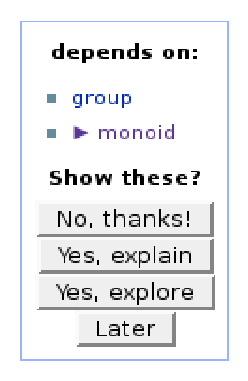
\includegraphics[width=2.5cm]{projects/swim/gui-showdeps}
\end{minipage}
\end{myfig}

\subsubsection{Further work}

Further work on {\swim} will concentrate on integrating a lightweight
management of change process.  Second, while the wiki is yet a user-friendly
\emph{browser}, there is still a demand for assisting users to \emph{edit}
{\omdoc}.  To this end, the {\qmath} preprocessor (see {\mysecref{qmath}}) will
be integrated into {\swim}.  Mathematical objects entered as {\qmath} will be
kept in this syntax for display in the edit form, but they will be converted to
{\omdoc} for rendering for presentation and when pages are exported to another
application.

%%% Local Variables: 
%%% mode: stex
%%% TeX-master: "../../omdoc"
%%% End: 

% LocalWords:  matwebsearch Ioan Sucan nC dx dy dt runningex XPointer ns attr
% LocalWords:  mq anyorder xmlns domainofapplication bvar ci cn eq OAI API da
% LocalWords:  Lange CPoint wikis dateness parseable isAuthorOf MediaWiki omdoc
% LocalWords:  aa wiki's Wiki wiki IkeWiki JA hypermedia elt semithick pres dg
% LocalWords:  elal gui showdeps qmath stex metadata wiki's scheint mir kein zu
% LocalWords:  Gegensatz sein

\end{projectdescription}

\begin{projectdescription}
  %%%%%%%%%%%%%%%%%%%%%%%%%%%%%%%%%%%%%%%%%%%%%%%%%%%%%%%%%%%%%%%%%%%%%%%%%
% This file is part of the LaTeX sources of the OMDoc 1.3 specifiation
% Copyright (c) 2006 Christoph Lange
% This work is licensed by the Creative Commons Share-Alike license
% see http://creativecommons.org/licenses/by-sa/2.5/ for details
\svnInfo $Id: main.tex 8453 2009-08-04 09:58:26Z kohlhase $
\svnKeyword $HeadURL: https://svn.omdoc.org/repos/omdoc/branches/omdoc-1.3/doc/spec/projects/swim/main.tex $
%%%%%%%%%%%%%%%%%%%%%%%%%%%%%%%%%%%%%%%%%%%%%%%%%%%%%%%%%%%%%%%%%%%%%%%%%

\section{{\swim} -- An OMDoc-based Semantic Wiki}
\begin{project}{swim}{http://kwarc.eecs.iu-bremen.de/projects/swim}
\pauthors{Christoph Lange\and Michael Kohlhase}
\pinstitute{Computer Science, International University Bremen}
\end{project}

{\swim} is a semantic wiki for collaboratively building, editing and browsing a
mathematical knowledge base of {\omdoc} theories. Our long-term objective is to develop a
software that facilitates the creation of a shared, public collection of mathematical
knowledge and serves work groups of mathematicians as a tool for collaborative development
of new theories.  Even though the work reported here was initially motivated by solving
the MKM author's dilemma~\cite{KohKoh:cdad04}, we contend that the new application area
MKM can also contribute to the development of semantic wikis.

Technically, {\swim} is based on the semantic wiki engine
\scsys{IkeWiki}~\cite{schaffert06:ikewiki}, which was chosen because of its
modular design, its rich semantic web infrastructure, its user assistance for
annotations, and its orientation towards
learning~\cite{schaffert06:learning-with-semantic-wikis}.

\subsection{Semantic Wikis}

A wiki~\cite{LeuCun01:wikiway} is a web server
application that allows users to browse, create, and edit hyperlinked pages in a web
browser, usually using a simple text syntax.  In contrast to most content management
systems, wiki pages are accessible via an URL containing their title.  A new page can be
created by linking from an existent page to the page to be created.  This link will then
lead to an edit form.  Usually, anyone is allowed to edit pages on a wiki, but access can
be restricted.  Other characteristics of wikis include permanent storage of old page
versions (with facilities to display differences between two versions and to restore a
certain version), notification about recent changes, and full-text search.

Semantic
wikis~\cite{voelkel06:semanticwikistateoftheart,TolPas06:wikis-semantic-hypermedia}
enhance wikis by Semantic Web technologies, such as {\rdf}~\cite{LasSwi:rdf99} or
ontologies.  Usually one page represents one concept from a real-world domain, which has a
type, possibly some metadata, and typed links to other concepts.  For example, a link from
a wiki page about ``Life, the Universe and Everything'' to another page about Douglas
Adams could be typed as ``is author of''.  In terms of {\rdf}, this can be expressed by the
following subject--predicate--object triple,

\[
(\mbox{``Douglas Adams''},\;\mbox{isAuthorOf},\;\mbox{``Life, the Universe and
Everything''})
\]

where the \textit{isAuthorOf} relation would be defined in an ontology.  These links are
usually displayed in a navigation box next to the page contents. Semantic wikis only deal
with wiki text, not with mathematics, though some allow to embed mathematical formulae as
presentational-only {\TeX}.

{\swim} encourages users to collaborate: Non-mathematicians can collaborate in creating a
``Wikipedia of mathematics'' by compiling the knowledge available so far, while scientists
can collaboratively develop new theories.  Users get an immediate reward for many of their
contributions: Once they specify the type of a page or relations of one page to another,
this information will be displayed in a box of navigation links.  We intend to make the
data created in {\swim} usable for external services by offering an export facility for
{\omdoc} documents and by integrating them into {\swim}.  Mathematicians developing
theories will be assisted to retain an overview of theory dependencies in order not to
break them.  Social software services will further utilize the semantic information
available from the theories and from tracking the user interaction log (``Who did what on
which page when?'').  User feedback to pages can be extended to social bookmarking, which
is ``the practice of saving bookmarks [of Internet resources] to a public web site and
`tagging' them with keywords.''~\cite{lomas05:social-bookmarking} The more users tag a
certain resource, the higher a social bookmarking service will rank it.

The enhancements of the data model semantic wikis bring along --- compared to traditional
wikis --- are already present in the {\omdoc} format, so that an {\omdoc}-based wiki only
needs to operationalize their underlying meaning. For example, typed links, which are
implemented via an extension to the wiki syntax in \scsys{Semantic
  MediaWiki}~\cite{voelkel06:semanticwikipedia} or editable through a separate editor in
\scsys{IkeWiki}~\cite{schaffert06:ikewiki}, are implemented by means of the \texttt{for}
attribute to {\omdoc}'s elements (e.g.\ \texttt{<example for="\#id-of-assertion">}).
{\swim} makes them editable easily and visualizes them adequately.  A semantic wiki
targeted at mathematics must ensure that dependencies between concepts are preserved.
Results in this area will be interesting for non-mathematical semantic wikis as well,
especially when they support higher levels of formalization such as ontologies.

\subsection{Design of {\swim}}

\subsubsection{Concepts and Relations}

The smallest unit that can be displayed, edited, linked to, or archived in a wiki is a
page. In a semantic wiki, it usually describes one {\emph{concept}}, including its
properties and its relations to other concepts.  While standalone {\omdoc} documents can
contain more than one theory, is is important to keep pages small in a wiki to improve the
effectivity of usage.  Furthermore, usual semantic wikis only store and display metadata
and typed links per page; {\swim} does too.\footnote{Semantic information will only be
  considered on the theory and statement levels of {\omdoc} --- directly or through
  reasoning in the case of transitive closures ---, not on the object level.}  Users are
strongly encouraged to define at most one theory per wiki page and to roll out
non-constitutive statements (see {\mysecref{statements-constitutive}}) to separate pages,
referencing their context theory.  As constitutive statements cannot exist without an
enclosing theory, but as, on the other hand, we want each wiki page to form a valid
document, we introduced a new element {\element[ns-elt=swim]{page}}, which can be a child
of an {\element{omdoc}} element and which has the same content model as a
{\element{theory}} element --- in particular, it can hold several theory-constitutive
statements and connect them to their context theory.
\begin{wrapfigure}{r}{8cm}
  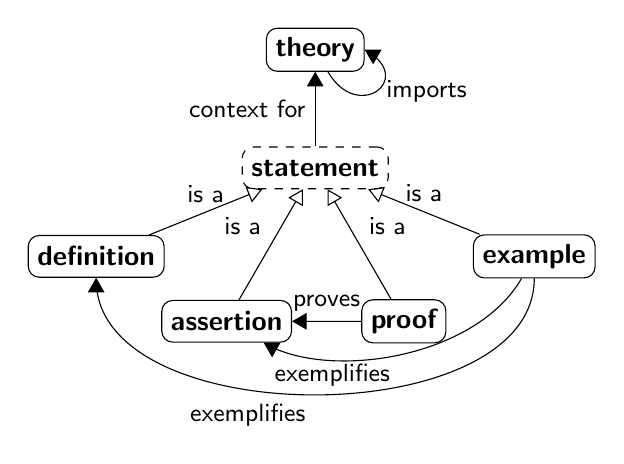
\begin{tikzpicture}[scale=1.5,thin,font=\sffamily,>=triangle 60]
    \tikzstyle{concept}=[font=\sffamily\bfseries,draw,minimum height=3.5ex,rounded corners]
    \tikzstyle{every path}=[font=\small\sffamily];
    \node[concept] (t) at (0,1) {theory};
    \node[concept,dashed] (s) at (0,0) {\itshape statement};
    \node[concept] (d) at +(-158:2.0cm) {definition};
    \begin{scope}[shift={(d)}]% control point for e->d
      \coordinate (da) at +(-90:1.5cm);% relative to s, not to a!
    \end{scope}
    \node[concept] (a) at +(-120:1.5cm) {assertion};
    \begin{scope}[shift={(a)}]% control point for e->a
      \coordinate (aa) at +(-30:1cm);% relative to s, not to a!
    \end{scope}
    \node[concept] (p) at +(-60:1.5cm) {proof};
    \node[concept] (e) at +(-22:2.0cm) {example};
    \draw[->] (t.-60) .. controls +(-60:0.5cm) and +(-30:0.5cm) .. node[right]
    {imports} (t.east);
    \draw[->] (s) -- node[left] {context for} (t);
    \draw[-open triangle 60] (d) -- node[above] {is a} (s);
    \draw[-open triangle 60] (a) -- node[above left] {is a} (s);
    \draw[-open triangle 60] (p) -- node[above right] {is a} (s);
    \draw[-open triangle 60] (e) -- node[above] {is a} (s);
    \draw[->] (p) -- node[above] {proves} (a);
    \draw[->] (e) ..
    controls +(-120:1cm)
    and (aa) ..
    node[below left] {exemplifies} (a);
    \draw[->] (e) ..
    controls +(-90:1.5cm)
    and (da) ..
    node[below left] {exemplifies} (d);
  \end{tikzpicture}
  \caption{Subset of {\omdoc}'s system ontology}\vspace*{-.5cm}
\end{wrapfigure}
{\omdoc}'s system ontology has been partly coded in OWL-DL and imported to the wiki's {\rdf}
store, which is implemented using the Jena Semantic Web Framework for
Java~\cite{URL:jena:web}. Theories as well as statements of any type form concepts, and
the most important relations between those concepts are extracted from the {\omdoc} pages
on saving and then stored as {\rdf} triples.  These relations include:
\begin{itemize}
\item The import relation between theories
\item The relation of a statement to its context theory
\item The relation of an example to the statement it exemplifies
\item The relation of a proof to the assertion it proves
\end{itemize}
It is planned to also take relations given by user interaction into consideration, such as
``Who edited which page when?'', and to combine ontology-defined relations and user
relations.  For example, a metric estimating the {\emph{degree of difficulty}} of a page,
calculated by counting the questions on the discussion page, could be implemented.
Furthermore, the user can specify taxonomic relations, which cannot be stated explicitly
in {\omdoc}, such as (``all differentiable functions are continuous''), as annotations in
an ontology language like {\rdf} Schema or {\owl}.

\subsubsection{User Interface and Interaction Model}

Pages can be rendered to XHTML plus presentational MathML using the transformations
described in {\mychapref{transform-xsl}}. There is also a browsable source code view, which is
useful for documents that are not written in textbook style.

Not only will the user be able to navigate along the dependency graph, she will also be
able to {\emph{interact}} with the system: she will be asked whether she wants to explore
the theories required as dependencies in further detail.

Suppose that the user is currently reading the page containing the theory {\snippet{ring}}
from the elementary algebra example from {\mychapref{dg-elal}}. In this case the wiki will
not only display navigation links to the direct dependencies {\snippet{group}} and
{\snippet{monoid}}, but it will also provide unobtrusive buttons that allow the user to
give one of the commands in {\myfigref{gui-showdeps}}. Not only the last case will be
recorded --- the others are interesting as well for \emph{social bookmarking}.  For
example, if many users requested a theory $t$ to be explained, the system could default to
display not only the direct dependencies but also the level-two dependencies, for it seems
that $t$ is too difficult for only being explained shallowly.

\begin{myfig}{gui-showdeps}{The command buttons to navigate along the dependencies}
  \begin{minipage}{8cm}
\begin{description}
\item[{\bf{No, thanks!}}] ``{\emph{I already know group and monoid.}}''
\item[{\bf{Explain}}] ``{\emph{Please show me group and monoid, I want to learn about
      ring's prerequisites.}}'' --- group and monoid will be displayed.
\item[{\bf{Explore}}] ``{\emph{Please show me {\emph{all}} prerequisites for ring.}}'' ---
  group, monoid, and semigroup, are opened in separate windows or serialized into one
  page.
\item[{\bf{Suspend}}] ``{\emph{I want to know about group and monoid, but only later.}}''
  --- {\swim} keeps a notice in the user's profile that she wants to read group and monoid
  sometime.  Reminder links to suspended theories are shown on a separate navigation bar.
\end{description}
\end{minipage}\quad
\begin{minipage}{2.5cm}
  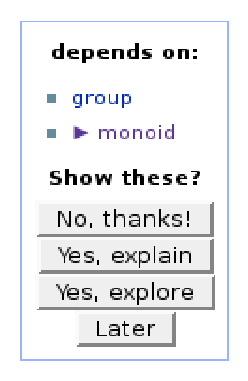
\includegraphics[width=2.5cm]{projects/swim/gui-showdeps}
\end{minipage}
\end{myfig}

\subsubsection{Further work}

Further work on {\swim} will concentrate on integrating a lightweight
management of change process.  Second, while the wiki is yet a user-friendly
\emph{browser}, there is still a demand for assisting users to \emph{edit}
{\omdoc}.  To this end, the {\qmath} preprocessor (see {\mysecref{qmath}}) will
be integrated into {\swim}.  Mathematical objects entered as {\qmath} will be
kept in this syntax for display in the edit form, but they will be converted to
{\omdoc} for rendering for presentation and when pages are exported to another
application.

%%% Local Variables: 
%%% mode: stex
%%% TeX-master: "../../omdoc"
%%% End: 

% LocalWords:  matwebsearch Ioan Sucan nC dx dy dt runningex XPointer ns attr
% LocalWords:  mq anyorder xmlns domainofapplication bvar ci cn eq OAI API da
% LocalWords:  Lange CPoint wikis dateness parseable isAuthorOf MediaWiki omdoc
% LocalWords:  aa wiki's Wiki wiki IkeWiki JA hypermedia elt semithick pres dg
% LocalWords:  elal gui showdeps qmath stex metadata wiki's scheint mir kein zu
% LocalWords:  Gegensatz sein

\end{projectdescription}

\begin{projectdescription}
  %%%%%%%%%%%%%%%%%%%%%%%%%%%%%%%%%%%%%%%%%%%%%%%%%%%%%%%%%%%%%%%%%%%%%%%%%
% This file is part of the LaTeX sources of the OMDoc 1.3 specifiation
% Copyright (c) 2006 Christoph Lange
% This work is licensed by the Creative Commons Share-Alike license
% see http://creativecommons.org/licenses/by-sa/2.5/ for details
\svnInfo $Id: main.tex 8453 2009-08-04 09:58:26Z kohlhase $
\svnKeyword $HeadURL: https://svn.omdoc.org/repos/omdoc/branches/omdoc-1.3/doc/spec/projects/swim/main.tex $
%%%%%%%%%%%%%%%%%%%%%%%%%%%%%%%%%%%%%%%%%%%%%%%%%%%%%%%%%%%%%%%%%%%%%%%%%

\section{{\swim} -- An OMDoc-based Semantic Wiki}
\begin{project}{swim}{http://kwarc.eecs.iu-bremen.de/projects/swim}
\pauthors{Christoph Lange\and Michael Kohlhase}
\pinstitute{Computer Science, International University Bremen}
\end{project}

{\swim} is a semantic wiki for collaboratively building, editing and browsing a
mathematical knowledge base of {\omdoc} theories. Our long-term objective is to develop a
software that facilitates the creation of a shared, public collection of mathematical
knowledge and serves work groups of mathematicians as a tool for collaborative development
of new theories.  Even though the work reported here was initially motivated by solving
the MKM author's dilemma~\cite{KohKoh:cdad04}, we contend that the new application area
MKM can also contribute to the development of semantic wikis.

Technically, {\swim} is based on the semantic wiki engine
\scsys{IkeWiki}~\cite{schaffert06:ikewiki}, which was chosen because of its
modular design, its rich semantic web infrastructure, its user assistance for
annotations, and its orientation towards
learning~\cite{schaffert06:learning-with-semantic-wikis}.

\subsection{Semantic Wikis}

A wiki~\cite{LeuCun01:wikiway} is a web server
application that allows users to browse, create, and edit hyperlinked pages in a web
browser, usually using a simple text syntax.  In contrast to most content management
systems, wiki pages are accessible via an URL containing their title.  A new page can be
created by linking from an existent page to the page to be created.  This link will then
lead to an edit form.  Usually, anyone is allowed to edit pages on a wiki, but access can
be restricted.  Other characteristics of wikis include permanent storage of old page
versions (with facilities to display differences between two versions and to restore a
certain version), notification about recent changes, and full-text search.

Semantic
wikis~\cite{voelkel06:semanticwikistateoftheart,TolPas06:wikis-semantic-hypermedia}
enhance wikis by Semantic Web technologies, such as {\rdf}~\cite{LasSwi:rdf99} or
ontologies.  Usually one page represents one concept from a real-world domain, which has a
type, possibly some metadata, and typed links to other concepts.  For example, a link from
a wiki page about ``Life, the Universe and Everything'' to another page about Douglas
Adams could be typed as ``is author of''.  In terms of {\rdf}, this can be expressed by the
following subject--predicate--object triple,

\[
(\mbox{``Douglas Adams''},\;\mbox{isAuthorOf},\;\mbox{``Life, the Universe and
Everything''})
\]

where the \textit{isAuthorOf} relation would be defined in an ontology.  These links are
usually displayed in a navigation box next to the page contents. Semantic wikis only deal
with wiki text, not with mathematics, though some allow to embed mathematical formulae as
presentational-only {\TeX}.

{\swim} encourages users to collaborate: Non-mathematicians can collaborate in creating a
``Wikipedia of mathematics'' by compiling the knowledge available so far, while scientists
can collaboratively develop new theories.  Users get an immediate reward for many of their
contributions: Once they specify the type of a page or relations of one page to another,
this information will be displayed in a box of navigation links.  We intend to make the
data created in {\swim} usable for external services by offering an export facility for
{\omdoc} documents and by integrating them into {\swim}.  Mathematicians developing
theories will be assisted to retain an overview of theory dependencies in order not to
break them.  Social software services will further utilize the semantic information
available from the theories and from tracking the user interaction log (``Who did what on
which page when?'').  User feedback to pages can be extended to social bookmarking, which
is ``the practice of saving bookmarks [of Internet resources] to a public web site and
`tagging' them with keywords.''~\cite{lomas05:social-bookmarking} The more users tag a
certain resource, the higher a social bookmarking service will rank it.

The enhancements of the data model semantic wikis bring along --- compared to traditional
wikis --- are already present in the {\omdoc} format, so that an {\omdoc}-based wiki only
needs to operationalize their underlying meaning. For example, typed links, which are
implemented via an extension to the wiki syntax in \scsys{Semantic
  MediaWiki}~\cite{voelkel06:semanticwikipedia} or editable through a separate editor in
\scsys{IkeWiki}~\cite{schaffert06:ikewiki}, are implemented by means of the \texttt{for}
attribute to {\omdoc}'s elements (e.g.\ \texttt{<example for="\#id-of-assertion">}).
{\swim} makes them editable easily and visualizes them adequately.  A semantic wiki
targeted at mathematics must ensure that dependencies between concepts are preserved.
Results in this area will be interesting for non-mathematical semantic wikis as well,
especially when they support higher levels of formalization such as ontologies.

\subsection{Design of {\swim}}

\subsubsection{Concepts and Relations}

The smallest unit that can be displayed, edited, linked to, or archived in a wiki is a
page. In a semantic wiki, it usually describes one {\emph{concept}}, including its
properties and its relations to other concepts.  While standalone {\omdoc} documents can
contain more than one theory, is is important to keep pages small in a wiki to improve the
effectivity of usage.  Furthermore, usual semantic wikis only store and display metadata
and typed links per page; {\swim} does too.\footnote{Semantic information will only be
  considered on the theory and statement levels of {\omdoc} --- directly or through
  reasoning in the case of transitive closures ---, not on the object level.}  Users are
strongly encouraged to define at most one theory per wiki page and to roll out
non-constitutive statements (see {\mysecref{statements-constitutive}}) to separate pages,
referencing their context theory.  As constitutive statements cannot exist without an
enclosing theory, but as, on the other hand, we want each wiki page to form a valid
document, we introduced a new element {\element[ns-elt=swim]{page}}, which can be a child
of an {\element{omdoc}} element and which has the same content model as a
{\element{theory}} element --- in particular, it can hold several theory-constitutive
statements and connect them to their context theory.
\begin{wrapfigure}{r}{8cm}
  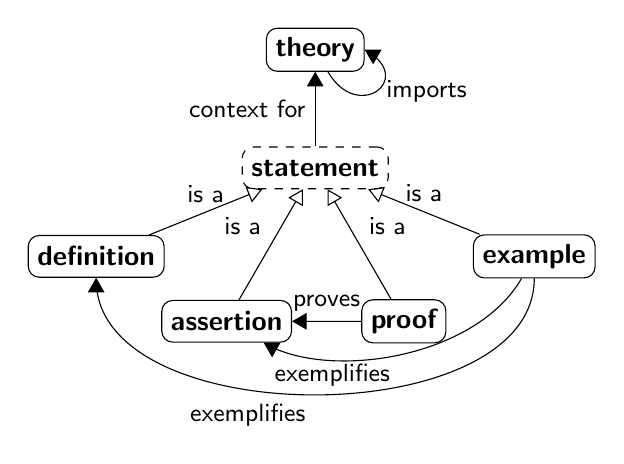
\begin{tikzpicture}[scale=1.5,thin,font=\sffamily,>=triangle 60]
    \tikzstyle{concept}=[font=\sffamily\bfseries,draw,minimum height=3.5ex,rounded corners]
    \tikzstyle{every path}=[font=\small\sffamily];
    \node[concept] (t) at (0,1) {theory};
    \node[concept,dashed] (s) at (0,0) {\itshape statement};
    \node[concept] (d) at +(-158:2.0cm) {definition};
    \begin{scope}[shift={(d)}]% control point for e->d
      \coordinate (da) at +(-90:1.5cm);% relative to s, not to a!
    \end{scope}
    \node[concept] (a) at +(-120:1.5cm) {assertion};
    \begin{scope}[shift={(a)}]% control point for e->a
      \coordinate (aa) at +(-30:1cm);% relative to s, not to a!
    \end{scope}
    \node[concept] (p) at +(-60:1.5cm) {proof};
    \node[concept] (e) at +(-22:2.0cm) {example};
    \draw[->] (t.-60) .. controls +(-60:0.5cm) and +(-30:0.5cm) .. node[right]
    {imports} (t.east);
    \draw[->] (s) -- node[left] {context for} (t);
    \draw[-open triangle 60] (d) -- node[above] {is a} (s);
    \draw[-open triangle 60] (a) -- node[above left] {is a} (s);
    \draw[-open triangle 60] (p) -- node[above right] {is a} (s);
    \draw[-open triangle 60] (e) -- node[above] {is a} (s);
    \draw[->] (p) -- node[above] {proves} (a);
    \draw[->] (e) ..
    controls +(-120:1cm)
    and (aa) ..
    node[below left] {exemplifies} (a);
    \draw[->] (e) ..
    controls +(-90:1.5cm)
    and (da) ..
    node[below left] {exemplifies} (d);
  \end{tikzpicture}
  \caption{Subset of {\omdoc}'s system ontology}\vspace*{-.5cm}
\end{wrapfigure}
{\omdoc}'s system ontology has been partly coded in OWL-DL and imported to the wiki's {\rdf}
store, which is implemented using the Jena Semantic Web Framework for
Java~\cite{URL:jena:web}. Theories as well as statements of any type form concepts, and
the most important relations between those concepts are extracted from the {\omdoc} pages
on saving and then stored as {\rdf} triples.  These relations include:
\begin{itemize}
\item The import relation between theories
\item The relation of a statement to its context theory
\item The relation of an example to the statement it exemplifies
\item The relation of a proof to the assertion it proves
\end{itemize}
It is planned to also take relations given by user interaction into consideration, such as
``Who edited which page when?'', and to combine ontology-defined relations and user
relations.  For example, a metric estimating the {\emph{degree of difficulty}} of a page,
calculated by counting the questions on the discussion page, could be implemented.
Furthermore, the user can specify taxonomic relations, which cannot be stated explicitly
in {\omdoc}, such as (``all differentiable functions are continuous''), as annotations in
an ontology language like {\rdf} Schema or {\owl}.

\subsubsection{User Interface and Interaction Model}

Pages can be rendered to XHTML plus presentational MathML using the transformations
described in {\mychapref{transform-xsl}}. There is also a browsable source code view, which is
useful for documents that are not written in textbook style.

Not only will the user be able to navigate along the dependency graph, she will also be
able to {\emph{interact}} with the system: she will be asked whether she wants to explore
the theories required as dependencies in further detail.

Suppose that the user is currently reading the page containing the theory {\snippet{ring}}
from the elementary algebra example from {\mychapref{dg-elal}}. In this case the wiki will
not only display navigation links to the direct dependencies {\snippet{group}} and
{\snippet{monoid}}, but it will also provide unobtrusive buttons that allow the user to
give one of the commands in {\myfigref{gui-showdeps}}. Not only the last case will be
recorded --- the others are interesting as well for \emph{social bookmarking}.  For
example, if many users requested a theory $t$ to be explained, the system could default to
display not only the direct dependencies but also the level-two dependencies, for it seems
that $t$ is too difficult for only being explained shallowly.

\begin{myfig}{gui-showdeps}{The command buttons to navigate along the dependencies}
  \begin{minipage}{8cm}
\begin{description}
\item[{\bf{No, thanks!}}] ``{\emph{I already know group and monoid.}}''
\item[{\bf{Explain}}] ``{\emph{Please show me group and monoid, I want to learn about
      ring's prerequisites.}}'' --- group and monoid will be displayed.
\item[{\bf{Explore}}] ``{\emph{Please show me {\emph{all}} prerequisites for ring.}}'' ---
  group, monoid, and semigroup, are opened in separate windows or serialized into one
  page.
\item[{\bf{Suspend}}] ``{\emph{I want to know about group and monoid, but only later.}}''
  --- {\swim} keeps a notice in the user's profile that she wants to read group and monoid
  sometime.  Reminder links to suspended theories are shown on a separate navigation bar.
\end{description}
\end{minipage}\quad
\begin{minipage}{2.5cm}
  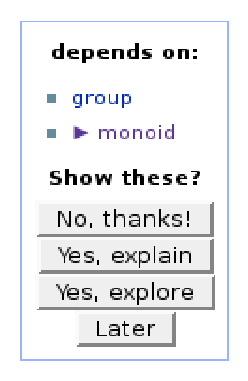
\includegraphics[width=2.5cm]{projects/swim/gui-showdeps}
\end{minipage}
\end{myfig}

\subsubsection{Further work}

Further work on {\swim} will concentrate on integrating a lightweight
management of change process.  Second, while the wiki is yet a user-friendly
\emph{browser}, there is still a demand for assisting users to \emph{edit}
{\omdoc}.  To this end, the {\qmath} preprocessor (see {\mysecref{qmath}}) will
be integrated into {\swim}.  Mathematical objects entered as {\qmath} will be
kept in this syntax for display in the edit form, but they will be converted to
{\omdoc} for rendering for presentation and when pages are exported to another
application.

%%% Local Variables: 
%%% mode: stex
%%% TeX-master: "../../omdoc"
%%% End: 

% LocalWords:  matwebsearch Ioan Sucan nC dx dy dt runningex XPointer ns attr
% LocalWords:  mq anyorder xmlns domainofapplication bvar ci cn eq OAI API da
% LocalWords:  Lange CPoint wikis dateness parseable isAuthorOf MediaWiki omdoc
% LocalWords:  aa wiki's Wiki wiki IkeWiki JA hypermedia elt semithick pres dg
% LocalWords:  elal gui showdeps qmath stex metadata wiki's scheint mir kein zu
% LocalWords:  Gegensatz sein

\end{projectdescription}

\begin{projectdescription}
  %%%%%%%%%%%%%%%%%%%%%%%%%%%%%%%%%%%%%%%%%%%%%%%%%%%%%%%%%%%%%%%%%%%%%%%%%
% This file is part of the LaTeX sources of the OMDoc 1.3 specifiation
% Copyright (c) 2006 Andrea Kohlhase
% This work is licensed by the Creative Commons Share-Alike license
% see http://creativecommons.org/licenses/by-sa/2.5/ for details
\svnInfo $Id: cpoint.tex 8453 2009-08-04 09:58:26Z kohlhase $
\svnKeyword $HeadURL: https://svn.omdoc.org/repos/omdoc/branches/omdoc-1.3/doc/spec/projects/cpoint/cpoint.tex $
%%%%%%%%%%%%%%%%%%%%%%%%%%%%%%%%%%%%%%%%%%%%%%%%%%%%%%%%%%%%%%%%%%%%%%%%%

\section[CPoint]{{\cpoint}: An {\omdoc} Editor in MS PowerPoint}
\def\cpauthor{\scsys{CPointAuthor}}
\def\cpstudent{\scsys{CPointStudent}}
\def\cpbasic{\scsys{CPointBasic}}
\def\cpgraphs{\scsys{CPointGraphs}}
\def\cpimport{\scsys{CPointImport}}
\def\cpnotes{\scsys{CPointNotes}}
\def\texpoint{\scsys{TexPoint}}

\begin{project}{cpoint}{http://kwarc.eecs.iu-bremen.de/software/CPoint/}
\pauthors{Andrea Kohlhase}
\pinstitute{Digital Media in Education (DiMeB), Dept. of Mathematics and Computer Science, University Bremen}
\end{project}

{\cpoint} is an invasive, semantic {\omdoc} editor in MS PowerPoint (with an {\omdoc}
outlet) that enables a user to distinguish between form and content in a document. As such
it can be viewed as an authoring tool for {\omdoc} documents with a focus on their
presentational potential. It enables a user to make implicit knowledge explicit. Moreover,
it provides several added-value services to a content author in order to alleviate the
short term costs of semantic mark up in contrast to its long term gains.

\subsection{The {\cpoint} Approach}\label{sec:background}
{\cpoint} started out as a part of the Course Capsules Project
({\ccaps}) at Carnegie Mellon University (2001 --- 2004), has been subsequently supported by the
International University Bremen (2004) and is now developed further at the '{\indextoo{Digital
    Media in Education}}' group at Bremen University. {\cpoint} is distributed under
the Gnu Lesser General Public License (LGPL)~\cite{LGPL}.  The newest version can be
downloaded from the project homepage.

PowerPoint ({\ppt}) slides address exclusively the issue of {\indextoo{presentation}} ---
the placement of text, symbols, and images on the screen, carefully sequenced and possibly
animated or embellished by sound. This directly leads to the question: {\emph{What exactly
    is the content in a {\ppt} presentation?}}

Obviously, the text and the pictures carry content as does the textual, presentational,
and placeholder structure.  For instance the ordering of information by writing it in list
form, grouping information bubbles in one slide, or marking text as title by putting it
into a 'title' placeholder can be mapped directly onto the {\omdoc} {\element{omgroup}}
and {\element{metadata}} elements.  Unfortunately though, this content exploits neither
{\omdoc}'s theory level nor the statement or formula level in more than a very superficial
way.

The 'real' content is hidden beneath the presentation form: the authors, lecturers, and
audience know or learn this real content by {\bf categorizing} what they see, and {\bf
  combining} it with what they already know and presently hear. {\cpoint} stands for '{\twintoo{Content in }{PowerPoint}}'. It models this by
providing the author with a tool to explicitly store the additional {\twintoo{implicit}{knowledge}}
with the {\ppt} show itself and from within the {\ppt} environment without destroying the
presentational aspects of the {\ppt} document. Moreover, {\cpoint} {\bf converts} the
additional content to the appropriate {\omdoc} levels, so that the resulting {\omdoc}
document captures all content.  For an author the {\twintoo{semantic}{markup}} process is
a long-term investment. In order to alleviate the author's costs, {\cpoint} has
implemented several {\bf added-value services}.

\subsection{The {\cpoint} Application}\label{sec:cpoint-app}
{\cpoint} extends {\ppt}'s
presentational functionalities by semantic ones to get a handle on its visible and
invisible content. As an invasive editor (see~\cite{Kohlhase:ophcie95}) {\cpoint} makes these
{\atwintoo{semantic}{authoring}{tool}s} available through a {\indextoo{toolbar}} in the
{\ppt} menu (see {\myfigref{menubar}}) where they are available whenever {\ppt} is
running. {\cpoint} is written in Visual Basic for Applications and can be distributed as a
{\ppt} add-in.

\begin{myfig}{menubar}{The {\cpoint} Menu Bar}
  
\includegraphics[width=11cm]{projects/cpoint/CPointMenuBar}
\end{myfig}

The top-level structure of a {\ppt} presentation is given by slides.  Each slide contains
{\bf {\ppt} objects}, e.g. text boxes, shapes, images, or tables. These objects carry
certain properties like text structure (e.g. ordered lists), document structure
(e.g. being a title in the text hierarchy), or presentational structure (e.g. color, bold
font, italic font, or symbol font). {\cpoint} enables the author to attach additional
information to each {\ppt} object. In particular, the author is empowered to transform
implicit into explicit knowledge by categorizing, combining and enhancing these objects semantically.

\paragraph{Categorizing}\label{sec:annotationform}
The semantic annotation process typically starts with understanding an object's role in
the to be transmitted knowledge and a subsequent categorization. The author selects the
respective {\ppt} object and assigns a suitable (didactic) role and category from a
pre-defined list ranging from hard core mathematical categories like ``Theory'',
``Definition'', or ``Assertion'' to didactic elements like ``Question'' or ``Comment''. If a {\ppt} object is part of a
multi-part presentation (e.g. ranging over multiple slides) of a semantic entity, it can
be marked as a sequel and inherits all information from previous parts. This way the
{\ppt} dependant linearity of the objects can be overcome.

\paragraph{Combining}\label{sec:detailsform}
For categorized {\ppt} objects the author can input category specific content via the
respective details form (see {\myfigref{Content}} as an example for a {\ppt} group
categorized as ``Axiom''). In particular, {\ppt} objects can be assigned a relation via
{\cpoint}'s reference system. For instance, the axiom in {\myfigref{Content}} sits in the
theory called `taxonomy of shapes'. A more sophisticated example would be a proof
{\emph{for}} an assertion that is constructed out of several, individual proof steps
succeeding one another.  Frequently, an author wants to reference implicit knowledge (e.g.
theories can comprise entire concepts and as such are typically not explicitly presented
in a lecture). Here, she can use {\cpoint} to create abstract {\ppt} objects called {\bf
  abstract objects} that are invisible in the actual {\ppt} show but can be dealt with like all other {\ppt} objects.

\begin{myfig}{Content}{The {\cpoint} Content Form for an Axiom Object}
  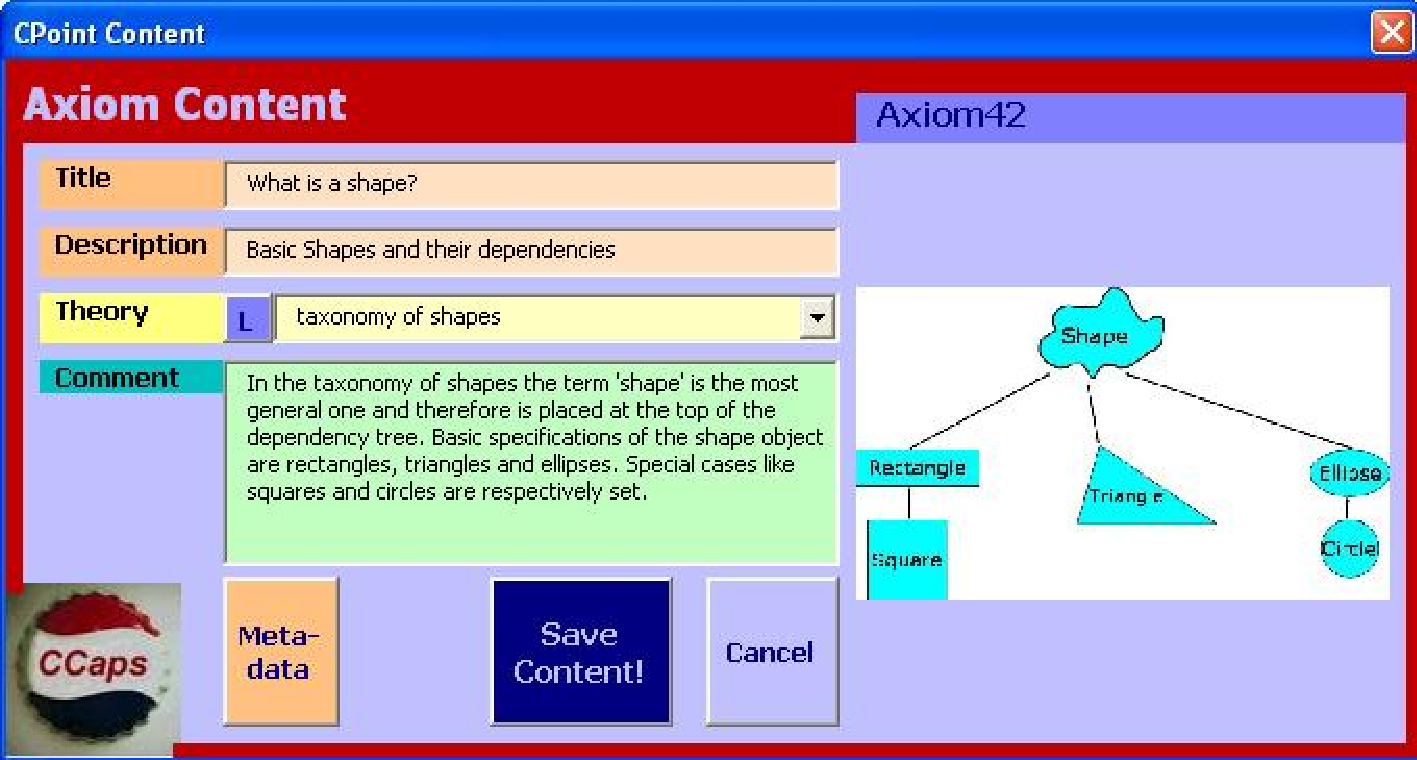
\includegraphics[width=9cm]{projects/cpoint/CPointContent}
\end{myfig}
The information annotated in these processes can be exploited for
added-value services.

\paragraph{{\omdoc} Conversion}\label{sec:omdocize} The heart of {\cpoint} is the
functionality for converting a fully ({\cpoint}-)edited presentation into a valid {\omdoc}
document.  This generated {\omdoc} document can for instance be read into
computer-supported education systems like {\activemath} (see~\cite{activemathAIEDJ01} and
{\mysecref{activemath}}).

\paragraph{Added-Value Services}\label{sec:auxiliaries}
As author support is essential for the motivation doing the semantic markup process,
{\cpoint} offers the following added-value services:
\begin{description}
\item[{\bf{Content Search and
      Navigation}\twin{content}{search}\twin{content}{navigation}}] {\cpoint}'s
  {\scsys{GoTo}} facility makes use of the additional semantic quality of {\ppt} objects
  by offering content search. For instance if an author remembers the existence of a
  definition of ``equivalence'' in some (older) {\ppt} presentation, she might look up all
  {\ppt} objects in a collection of several {\ppt} presentations that are categorized as
  ``Definition'' and whose title contain the word ``equivalence''. The author is offered a list
  of all these objects and by selecting one she is directed to the specific {\ppt} object.
\item[{\bf Dependency Graphs}\twin{dependency}{graph}] {\cpgraphs} enables the user to
  view graph based presentations of the annotated knowledge on distinct detail levels.
\item[{\bf Semantics-Induced Presentation}\twin{semantics-induced}{presentation}] The
  module {\cpauthor} offers the presentation of the underlying semantics. Whenever the
  author selects a {\ppt} object basic semantic information (like category, title, and
  main references) is presented to her. With {\cpoint}'s Visualize Mode semantic labels
  for annotated {\ppt} objects are generated.
\item[{\bf Creation of Pre-Categorized {\ppt} Objects}] Based on an individually designed
  CSS style sheet categorized, styled {\ppt} objects can be {\emph{created}} with
  {\cpauthor}. The layout is determined in the CSS file by the respective category (e.g.
  proposition) or superordinate classification (e.g. assertion, content, general).
\item[{\bf Math Glyphs in {\ppt}}\twin{mathematical}{glyph}] Based on the {\ppt} add-in
  {\texpoint}, the CMath functionalities empower an author to define individual symbol
  presentations. {\cpoint} introduces a mathematical user interface, which fully
  integrates mathematical symbols into PowerPoint presentations based on the semantics of
  the underlying objects rather than simply generating appropriate ink marks. For
  instance, the author might categorize a {\ppt} object as a symbol with the name 'reals'
  for the real numbers. The specific Unicode character to represent the real numbers can
  be declared with {\cpoint}. Subsequently, whenever the author writes the text
  '\verb|\reals|' and activates the math mode, then this sequence of characters is
  replaced by the previously declared presentation. The symbol presentation may also be
  given in {\LaTeX} form so that {\texpoint} can transform the {\LaTeX} code into {\ppt}
  glyphs. Note that this feature is not limited to math glyphs but can be used for handy
  abbreviations (macros) as well.
\item[{\bf Editorial Notes}\twin{editorial}{note}] Treating {\ppt} presentations as
  content documents requires more editing, therefore {\cpnotes} add editorial
  functionalities like grouped editorial notes and {\indextoo{navigation}} within these.
\item[{\bf {\omdoc} To {\ppt}}] The {\cpimport} module enables the import of {\omdoc}
  documents into the {\ppt} application. According to an individual underlying CSS style sheet {\ppt}
  objects in a newly created {\ppt} presentation are generated.
\item[{\bf ActiveMath}] Integrated development environment for ActiveMath content and
  specific ActiveMath book creation for a selected {\ppt} object.
\end{description}

\subsection{Future Work}
In the future the addition of other added-value services for users is planned. We want to
shift the focus from the authoring role to the recipient role of a {\ppt} presentation,
e.g. in form of a {\cpstudent} module in accordance with the {\cpauthor} module.
Furthermore, a new, more basic and therefore more user-friendly interface for {\cpoint}
novices will be implemented. This {\cpbasic} module will try to overcome the heavily
form-oriented format of {\cpoint}. In a next step the growing of a {\cpoint} user will be
supported by offering advanced {\cpoint} utilities that will extend {\cpbasic}.
Additionally, the success of ``social software'' under the Web 2.0 paradigm like ``social
bookmarking'' gives rise to the idea of a new personal and sharable {\ppt} objects
management where the predefined categories in {\cpoint} are replaced by ``social tags''.
Another {\cpoint} project is its extension for usage by teachers in school, which
usefulness has already been established in~\cite{Kohlhase:emPowerPoint}. The newest
project at the International University of Bremen is the implementation of a
{\cpoint}-like editor for MS Word.

%%% Local Variables: 
%%% mode: latex
%%% TeX-master: "../../omdoc"
%%% End: 

% LocalWords:  CPoint CPointAuthor CPointStudent CPointBasic CPointGraphs DiMeB
% LocalWords:  CPointImport CPointNotes TexPoint cpoint LGPL omgroup metadata
% LocalWords:  activemath GoTo CMath reals ActiveMath ActiveMath menubar

\end{projectdescription}

\begin{projectdescription}
  %%%%%%%%%%%%%%%%%%%%%%%%%%%%%%%%%%%%%%%%%%%%%%%%%%%%%%%%%%%%%%%%%%%%%%%%%
% This file is part of the LaTeX sources of the OMDoc 1.3 specifiation
% Copyright (c) 2006 Christoph Lange
% This work is licensed by the Creative Commons Share-Alike license
% see http://creativecommons.org/licenses/by-sa/2.5/ for details
\svnInfo $Id: main.tex 8453 2009-08-04 09:58:26Z kohlhase $
\svnKeyword $HeadURL: https://svn.omdoc.org/repos/omdoc/branches/omdoc-1.3/doc/spec/projects/swim/main.tex $
%%%%%%%%%%%%%%%%%%%%%%%%%%%%%%%%%%%%%%%%%%%%%%%%%%%%%%%%%%%%%%%%%%%%%%%%%

\section{{\swim} -- An OMDoc-based Semantic Wiki}
\begin{project}{swim}{http://kwarc.eecs.iu-bremen.de/projects/swim}
\pauthors{Christoph Lange\and Michael Kohlhase}
\pinstitute{Computer Science, International University Bremen}
\end{project}

{\swim} is a semantic wiki for collaboratively building, editing and browsing a
mathematical knowledge base of {\omdoc} theories. Our long-term objective is to develop a
software that facilitates the creation of a shared, public collection of mathematical
knowledge and serves work groups of mathematicians as a tool for collaborative development
of new theories.  Even though the work reported here was initially motivated by solving
the MKM author's dilemma~\cite{KohKoh:cdad04}, we contend that the new application area
MKM can also contribute to the development of semantic wikis.

Technically, {\swim} is based on the semantic wiki engine
\scsys{IkeWiki}~\cite{schaffert06:ikewiki}, which was chosen because of its
modular design, its rich semantic web infrastructure, its user assistance for
annotations, and its orientation towards
learning~\cite{schaffert06:learning-with-semantic-wikis}.

\subsection{Semantic Wikis}

A wiki~\cite{LeuCun01:wikiway} is a web server
application that allows users to browse, create, and edit hyperlinked pages in a web
browser, usually using a simple text syntax.  In contrast to most content management
systems, wiki pages are accessible via an URL containing their title.  A new page can be
created by linking from an existent page to the page to be created.  This link will then
lead to an edit form.  Usually, anyone is allowed to edit pages on a wiki, but access can
be restricted.  Other characteristics of wikis include permanent storage of old page
versions (with facilities to display differences between two versions and to restore a
certain version), notification about recent changes, and full-text search.

Semantic
wikis~\cite{voelkel06:semanticwikistateoftheart,TolPas06:wikis-semantic-hypermedia}
enhance wikis by Semantic Web technologies, such as {\rdf}~\cite{LasSwi:rdf99} or
ontologies.  Usually one page represents one concept from a real-world domain, which has a
type, possibly some metadata, and typed links to other concepts.  For example, a link from
a wiki page about ``Life, the Universe and Everything'' to another page about Douglas
Adams could be typed as ``is author of''.  In terms of {\rdf}, this can be expressed by the
following subject--predicate--object triple,

\[
(\mbox{``Douglas Adams''},\;\mbox{isAuthorOf},\;\mbox{``Life, the Universe and
Everything''})
\]

where the \textit{isAuthorOf} relation would be defined in an ontology.  These links are
usually displayed in a navigation box next to the page contents. Semantic wikis only deal
with wiki text, not with mathematics, though some allow to embed mathematical formulae as
presentational-only {\TeX}.

{\swim} encourages users to collaborate: Non-mathematicians can collaborate in creating a
``Wikipedia of mathematics'' by compiling the knowledge available so far, while scientists
can collaboratively develop new theories.  Users get an immediate reward for many of their
contributions: Once they specify the type of a page or relations of one page to another,
this information will be displayed in a box of navigation links.  We intend to make the
data created in {\swim} usable for external services by offering an export facility for
{\omdoc} documents and by integrating them into {\swim}.  Mathematicians developing
theories will be assisted to retain an overview of theory dependencies in order not to
break them.  Social software services will further utilize the semantic information
available from the theories and from tracking the user interaction log (``Who did what on
which page when?'').  User feedback to pages can be extended to social bookmarking, which
is ``the practice of saving bookmarks [of Internet resources] to a public web site and
`tagging' them with keywords.''~\cite{lomas05:social-bookmarking} The more users tag a
certain resource, the higher a social bookmarking service will rank it.

The enhancements of the data model semantic wikis bring along --- compared to traditional
wikis --- are already present in the {\omdoc} format, so that an {\omdoc}-based wiki only
needs to operationalize their underlying meaning. For example, typed links, which are
implemented via an extension to the wiki syntax in \scsys{Semantic
  MediaWiki}~\cite{voelkel06:semanticwikipedia} or editable through a separate editor in
\scsys{IkeWiki}~\cite{schaffert06:ikewiki}, are implemented by means of the \texttt{for}
attribute to {\omdoc}'s elements (e.g.\ \texttt{<example for="\#id-of-assertion">}).
{\swim} makes them editable easily and visualizes them adequately.  A semantic wiki
targeted at mathematics must ensure that dependencies between concepts are preserved.
Results in this area will be interesting for non-mathematical semantic wikis as well,
especially when they support higher levels of formalization such as ontologies.

\subsection{Design of {\swim}}

\subsubsection{Concepts and Relations}

The smallest unit that can be displayed, edited, linked to, or archived in a wiki is a
page. In a semantic wiki, it usually describes one {\emph{concept}}, including its
properties and its relations to other concepts.  While standalone {\omdoc} documents can
contain more than one theory, is is important to keep pages small in a wiki to improve the
effectivity of usage.  Furthermore, usual semantic wikis only store and display metadata
and typed links per page; {\swim} does too.\footnote{Semantic information will only be
  considered on the theory and statement levels of {\omdoc} --- directly or through
  reasoning in the case of transitive closures ---, not on the object level.}  Users are
strongly encouraged to define at most one theory per wiki page and to roll out
non-constitutive statements (see {\mysecref{statements-constitutive}}) to separate pages,
referencing their context theory.  As constitutive statements cannot exist without an
enclosing theory, but as, on the other hand, we want each wiki page to form a valid
document, we introduced a new element {\element[ns-elt=swim]{page}}, which can be a child
of an {\element{omdoc}} element and which has the same content model as a
{\element{theory}} element --- in particular, it can hold several theory-constitutive
statements and connect them to their context theory.
\begin{wrapfigure}{r}{8cm}
  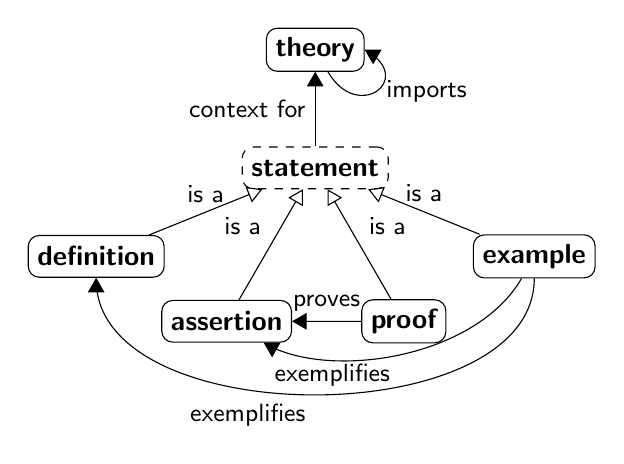
\begin{tikzpicture}[scale=1.5,thin,font=\sffamily,>=triangle 60]
    \tikzstyle{concept}=[font=\sffamily\bfseries,draw,minimum height=3.5ex,rounded corners]
    \tikzstyle{every path}=[font=\small\sffamily];
    \node[concept] (t) at (0,1) {theory};
    \node[concept,dashed] (s) at (0,0) {\itshape statement};
    \node[concept] (d) at +(-158:2.0cm) {definition};
    \begin{scope}[shift={(d)}]% control point for e->d
      \coordinate (da) at +(-90:1.5cm);% relative to s, not to a!
    \end{scope}
    \node[concept] (a) at +(-120:1.5cm) {assertion};
    \begin{scope}[shift={(a)}]% control point for e->a
      \coordinate (aa) at +(-30:1cm);% relative to s, not to a!
    \end{scope}
    \node[concept] (p) at +(-60:1.5cm) {proof};
    \node[concept] (e) at +(-22:2.0cm) {example};
    \draw[->] (t.-60) .. controls +(-60:0.5cm) and +(-30:0.5cm) .. node[right]
    {imports} (t.east);
    \draw[->] (s) -- node[left] {context for} (t);
    \draw[-open triangle 60] (d) -- node[above] {is a} (s);
    \draw[-open triangle 60] (a) -- node[above left] {is a} (s);
    \draw[-open triangle 60] (p) -- node[above right] {is a} (s);
    \draw[-open triangle 60] (e) -- node[above] {is a} (s);
    \draw[->] (p) -- node[above] {proves} (a);
    \draw[->] (e) ..
    controls +(-120:1cm)
    and (aa) ..
    node[below left] {exemplifies} (a);
    \draw[->] (e) ..
    controls +(-90:1.5cm)
    and (da) ..
    node[below left] {exemplifies} (d);
  \end{tikzpicture}
  \caption{Subset of {\omdoc}'s system ontology}\vspace*{-.5cm}
\end{wrapfigure}
{\omdoc}'s system ontology has been partly coded in OWL-DL and imported to the wiki's {\rdf}
store, which is implemented using the Jena Semantic Web Framework for
Java~\cite{URL:jena:web}. Theories as well as statements of any type form concepts, and
the most important relations between those concepts are extracted from the {\omdoc} pages
on saving and then stored as {\rdf} triples.  These relations include:
\begin{itemize}
\item The import relation between theories
\item The relation of a statement to its context theory
\item The relation of an example to the statement it exemplifies
\item The relation of a proof to the assertion it proves
\end{itemize}
It is planned to also take relations given by user interaction into consideration, such as
``Who edited which page when?'', and to combine ontology-defined relations and user
relations.  For example, a metric estimating the {\emph{degree of difficulty}} of a page,
calculated by counting the questions on the discussion page, could be implemented.
Furthermore, the user can specify taxonomic relations, which cannot be stated explicitly
in {\omdoc}, such as (``all differentiable functions are continuous''), as annotations in
an ontology language like {\rdf} Schema or {\owl}.

\subsubsection{User Interface and Interaction Model}

Pages can be rendered to XHTML plus presentational MathML using the transformations
described in {\mychapref{transform-xsl}}. There is also a browsable source code view, which is
useful for documents that are not written in textbook style.

Not only will the user be able to navigate along the dependency graph, she will also be
able to {\emph{interact}} with the system: she will be asked whether she wants to explore
the theories required as dependencies in further detail.

Suppose that the user is currently reading the page containing the theory {\snippet{ring}}
from the elementary algebra example from {\mychapref{dg-elal}}. In this case the wiki will
not only display navigation links to the direct dependencies {\snippet{group}} and
{\snippet{monoid}}, but it will also provide unobtrusive buttons that allow the user to
give one of the commands in {\myfigref{gui-showdeps}}. Not only the last case will be
recorded --- the others are interesting as well for \emph{social bookmarking}.  For
example, if many users requested a theory $t$ to be explained, the system could default to
display not only the direct dependencies but also the level-two dependencies, for it seems
that $t$ is too difficult for only being explained shallowly.

\begin{myfig}{gui-showdeps}{The command buttons to navigate along the dependencies}
  \begin{minipage}{8cm}
\begin{description}
\item[{\bf{No, thanks!}}] ``{\emph{I already know group and monoid.}}''
\item[{\bf{Explain}}] ``{\emph{Please show me group and monoid, I want to learn about
      ring's prerequisites.}}'' --- group and monoid will be displayed.
\item[{\bf{Explore}}] ``{\emph{Please show me {\emph{all}} prerequisites for ring.}}'' ---
  group, monoid, and semigroup, are opened in separate windows or serialized into one
  page.
\item[{\bf{Suspend}}] ``{\emph{I want to know about group and monoid, but only later.}}''
  --- {\swim} keeps a notice in the user's profile that she wants to read group and monoid
  sometime.  Reminder links to suspended theories are shown on a separate navigation bar.
\end{description}
\end{minipage}\quad
\begin{minipage}{2.5cm}
  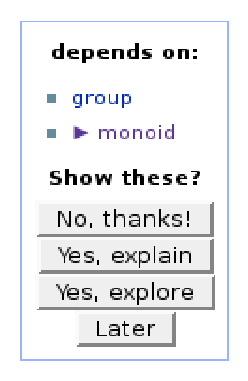
\includegraphics[width=2.5cm]{projects/swim/gui-showdeps}
\end{minipage}
\end{myfig}

\subsubsection{Further work}

Further work on {\swim} will concentrate on integrating a lightweight
management of change process.  Second, while the wiki is yet a user-friendly
\emph{browser}, there is still a demand for assisting users to \emph{edit}
{\omdoc}.  To this end, the {\qmath} preprocessor (see {\mysecref{qmath}}) will
be integrated into {\swim}.  Mathematical objects entered as {\qmath} will be
kept in this syntax for display in the edit form, but they will be converted to
{\omdoc} for rendering for presentation and when pages are exported to another
application.

%%% Local Variables: 
%%% mode: stex
%%% TeX-master: "../../omdoc"
%%% End: 

% LocalWords:  matwebsearch Ioan Sucan nC dx dy dt runningex XPointer ns attr
% LocalWords:  mq anyorder xmlns domainofapplication bvar ci cn eq OAI API da
% LocalWords:  Lange CPoint wikis dateness parseable isAuthorOf MediaWiki omdoc
% LocalWords:  aa wiki's Wiki wiki IkeWiki JA hypermedia elt semithick pres dg
% LocalWords:  elal gui showdeps qmath stex metadata wiki's scheint mir kein zu
% LocalWords:  Gegensatz sein

\end{projectdescription}

\begin{projectdescription}
  %%%%%%%%%%%%%%%%%%%%%%%%%%%%%%%%%%%%%%%%%%%%%%%%%%%%%%%%%%%%%%%%%%%%%%%%%
% This file is part of the LaTeX sources of the OMDoc 1.3 specifiation
% Copyright (c) 2006 Peter Jansen
% This work is licensed by the Creative Commons Share-Alike license
% see http://creativecommons.org/licenses/by-sa/2.5/ for details
\svnInfo $Id: report.tex 8453 2009-08-04 09:58:26Z kohlhase $
\svnKeyword $HeadURL: https://svn.omdoc.org/repos/omdoc/branches/omdoc-1.3/doc/spec/projects/omdocmode/report.tex $
%%%%%%%%%%%%%%%%%%%%%%%%%%%%%%%%%%%%%%%%%%%%%%%%%%%%%%%%%%%%%%%%%%%%%%%%%

\section{An Emacs mode for editing OMDoc Documents}
\begin{project}{omdocmode}{http://www.cs.cmu.edu/~ccaps}
\pauthors{Peter Jansen}
\pinstitute{School of Computer Science, Carnegie Mellon University}
\end{project}

We describe an {\emacs} major mode for editing {\omdoc} documents, developed by the {\scsys{Course Capsules}}
project group at the CMU School of Computer Science.  This mode extends the {\emacs}
editor~\cite{Stallman:em02} with functionality intended to help visualize, edit, and
create documents written in {\omdoc} format.

The mode is part of the {\omdoc} distribution (see {\mysecref{distribution}}), it is
provided under the conditions specified in the Library Gnu Public License~\cite{LGPL}.

\subsection{Introduction}

The CCaps project has developed tools to convert legacy materials written in a variety of
formats ({\scsys{PowerPoint}}, {\mathematica}, etc.)  into the {\omdoc} format (see
{\mysecsref{cpoint}{nb2omdoc}}). In many cases the output generated by such tools needs to
be post-processed or otherwise modified.

To this end, a user must open the file, read and understand its contents and perform the
appropriate modifications.  Though an {\omdoc} document is a regular text file, most of
its content consists of markup, which is hard to read and tedious to type.  It is
therefore important to support the user with tools that make a document easier to read and
modify, either in the form of a separate editor, or as an extension of an existing editor.

One approach to this is to build a {\emph{visual {\omdoc} editor}}, which presents the
document in a form resembling conventional mathematical documents (i.e., without showing
the markup explicitly, and with appropriate formatting for mathematical formulae), and
offers the user functionality to modify or annotate its content.

While this is ideal for user understanding of document content, it presupposes
consistent syntactic correctness, makes it more difficult to inspect or change
markup directly, and may present challenges as to resolving user action
ambiguities.

We have taken this approach in the {\cpoint} and {\mathematica} add-ins (see
{\mysecsref{cpoint}{nb2omdoc}}). But we also wanted a tool that would maintain full
control of all the textual information, while offering support for readability and editing
functionality.  We chose for this tool to extend the {\emacs} editor~\cite{Stallman:em02},
which lends itself very well to this task (as well as being the editor for general use for
several of our group).

\subsection{{\omdoc} mode functionality}

We now look at the different categories of
functionality in slightly more detail.

\paragraph{Visualization}
is currently provided by the use of the {\emacs} {\emph{font-lock}} mechanism to give
different categories of tags and content different fonts and colors to make them easily
recognizable.  Element categories currently recognized correspond to the {\omdoc} 1.2
modules: Document structure, Math, Theories, Auxiliaries, Presentation, {\openmath}, and
the {\indextoo{Dublin Core}} elements.

A customizable {\emph{indentation function}} allows for intelligible layout, which is
helpful both in hand-coding and the editing of the output of a legacy transformation
process.  There are key bindings for line, region, and enclosing element indentation.

\paragraph{Editing}
Functionality consists mainly of automated insertion of {\emph{templates}} for each of the
{\omdoc} elements, both via mode-dependent menu options and key bindings, grouped by
element category (the same categories as given above).

The template insertion mechanism is based on {\snippet{tempo.el}}, which allows for the
maintenance of a {\emph{list of insertion points}} the user can navigate in between to
supply or change the values of certain attributes.

The main function currently available for completing incomplete elements is the equivalent
of the standard {\snippet{electric-/}} function.  We are planning to add several other
completion functions in the near future (for tags, tag sets, attribute names, and symbol
and theory names).

The mode also provides for {\emph{validation}}: either internally (as a simple local
syntax check to check well-formedness) or externally (via an external xml validation
validation engine).  Internal validation builds an abbreviated parse tree, and highlights
discrepancies, suggesting possible modifications of insertions of element opening or
closing tags.  External validation runs an external xml validation engine ({\rxp} or
{\nsgmls}, depending on the configuration variables), and shows the output in a separate
buffer.

\begin{myfig}{skeleton}{Opening a new Buffer in {\omdoc} Mode}
  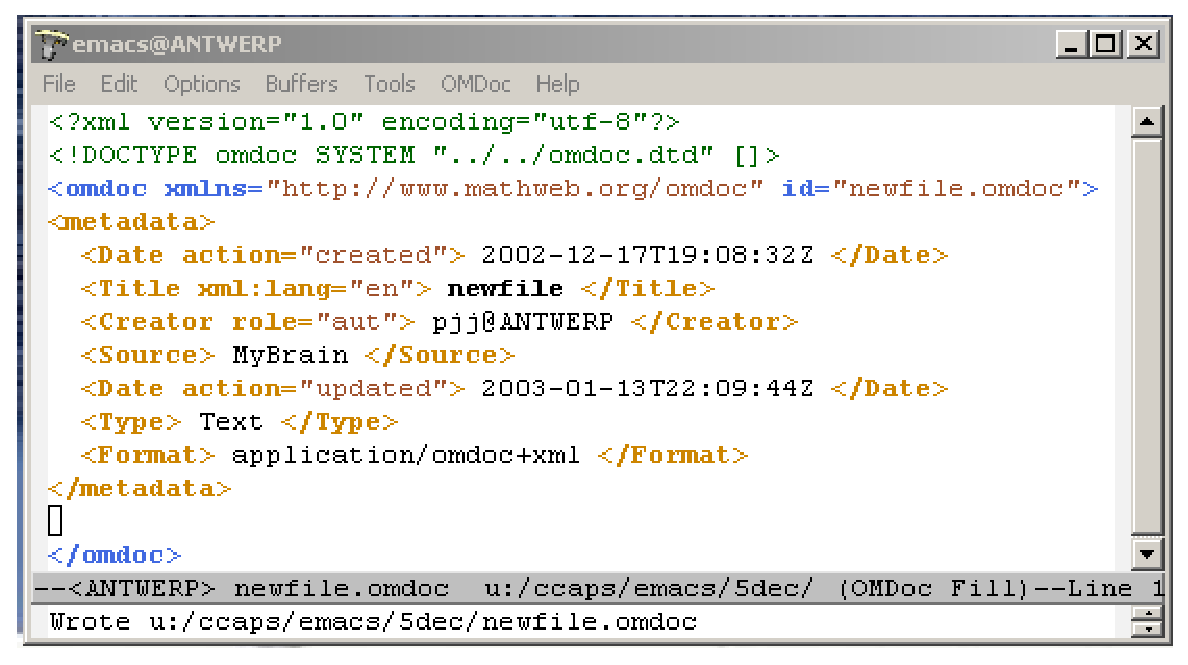
\includegraphics[width=9cm]{projects/omdocmode/omdoc2c}
\end{myfig}

\paragraph{Document creation}
is supported by automatic insertion of a basic {\emph{{\omdoc} skeleton}} in new buffers
as well as a {\emph{time-stamp updating}} mechanism and some smaller functions that extract
information from the user's environment variables to supply information for some of the
metadata slots (see the example in {\myfigref{skeleton}} below).

\subsection{Examples}

We illustrate some of the above by means of a few screen shots.  The example in
{\myfigref{menu}} is taken while editing a document that was semi-automatically generated
from part of a {\mathematica} notebook~(\cite{Sutner:cmnto04}).  Here, the user has
already run an automated indentation function, for example by activating
{\snippet{omdoc-indent-enclosing-main}} by typing {\snippet{C-c C-q}}, and is now about to
use the {\omdoc} menu to enter a new construct.


\begin{myfig}{menu}{Editing an {\omdoc} Document}
  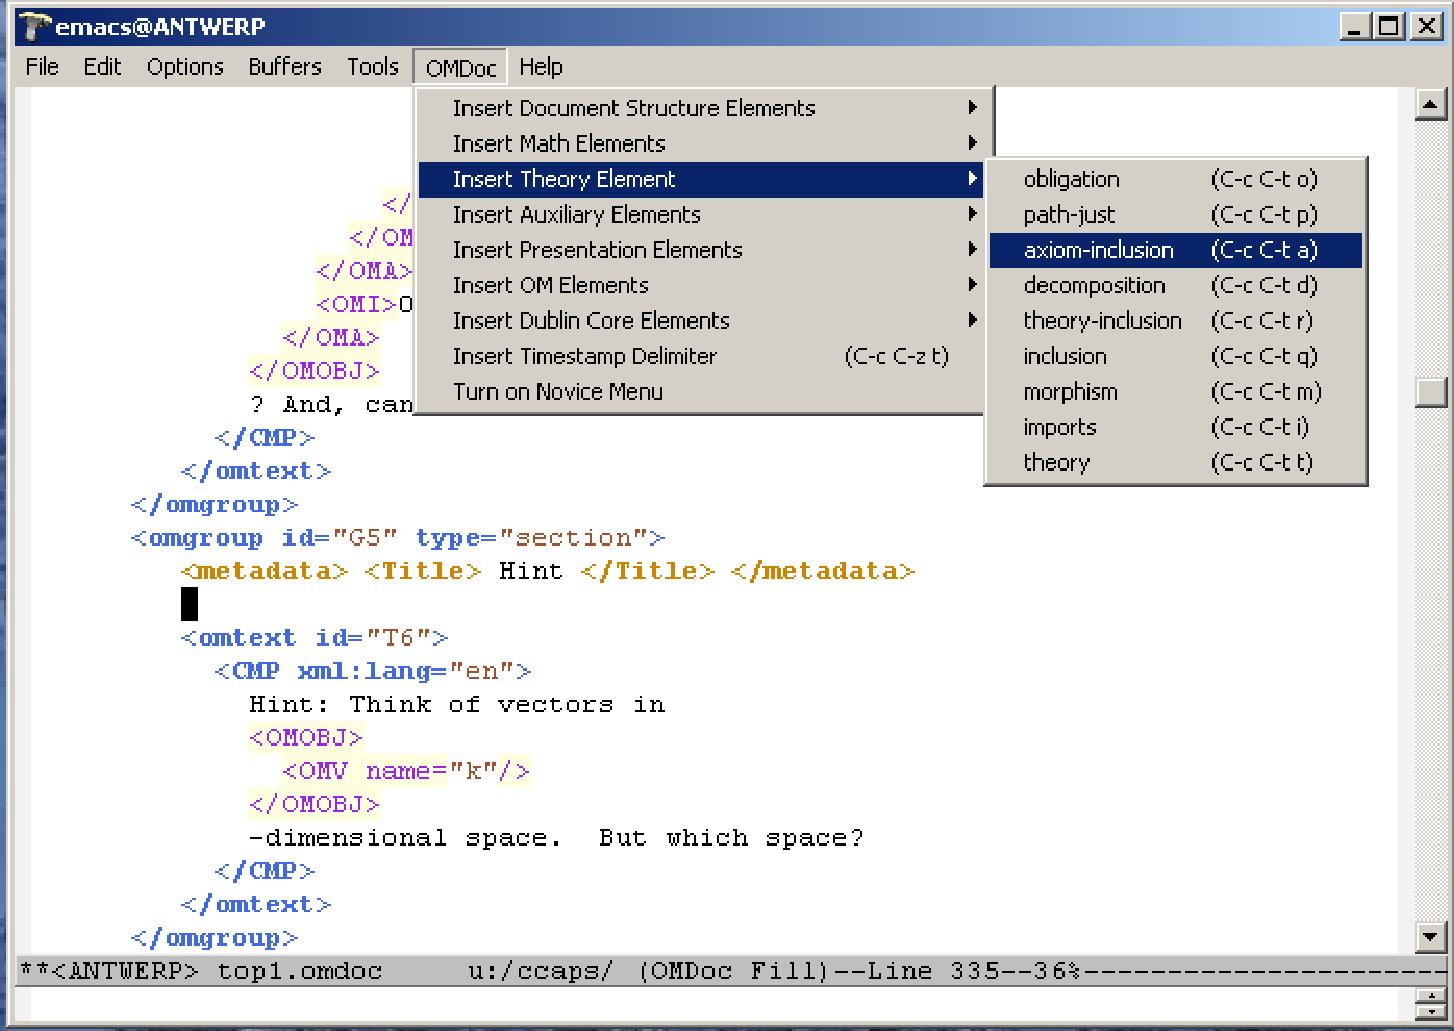
\includegraphics[width=9cm]{projects/omdocmode/omdoc1c}
\end{myfig}

After this operation, which could also have been performed by typing the key sequence
{\snippet{C-c C-t a}}), {\emacs} inserts the following text at the point (i.e. cursor
position).
\begin{lstlisting}
<axiom-inclusion xml:id="" to=""> </axiom-inclusion>
\end{lstlisting}

The second example shows the skeleton template that is automatically inserted when the
user opens a new file: {\myfigref{skeleton}}.  Note that the file name has been used as id
and title automatically, and the user's address appears in the Author field.  Timestamps
are inserted in Date fields for both creation and update, and the latter is adjusted
automatically every time changes are saved to the file.

%%% Local Variables: 
%%% mode: latex
%%% TeX-master: "../../omdoc"
%%% End: 

% LocalWords:  omdocmode el CCaps cpoint nb omdoc metadata

\end{projectdescription}

\begin{projectdescription}
  %%%%%%%%%%%%%%%%%%%%%%%%%%%%%%%%%%%%%%%%%%%%%%%%%%%%%%%%%%%%%%%%%%%%%%%%%
% This file is part of the LaTeX sources of the OMDoc 1.3 specifiation
% Copyright (c) 2006 Klaus Sutner
% This work is licensed by the Creative Commons Share-Alike license
% see http://creativecommons.org/licenses/by-sa/2.5/ for details
\svnInfo $Id: nb2omdoc.tex 8453 2009-08-04 09:58:26Z kohlhase $
\svnKeyword $HeadURL: https://svn.omdoc.org/repos/omdoc/branches/omdoc-1.3/doc/spec/projects/mathematica/nb2omdoc.tex $
%%%%%%%%%%%%%%%%%%%%%%%%%%%%%%%%%%%%%%%%%%%%%%%%%%%%%%%%%%%%%%%%%%%%%%%%%
\def\nb2om{\scsys{nb2omdoc}}

\section{Converting Mathematica Notebooks to OMDoc}
\begin{project}{nb2omdoc}{http://www.cs.cmu.edu/~ccaps}
\pauthors{Klaus Sutner}
\pinstitute{School of Computer Science, Carnegie Mellon University}
\end{project}

We describe a tool that converts {\mathematica} notebooks to {\omdoc}.  The program is
implemented entirely in {\mathematica} and easily extensible.

Creating an editor for general mathematical documents is notoriously difficult, in
particular when input methods are required that mimic the traditional two-dimensional
layout of many formulae.  Thus, it seems natural to use an existing high-quality system
such as the {\mathematica} notebook front end as an authoring tool for mathematical
documents.  A considerable amount of effort has gone into the design of this front end, see
for example~\cite{Wolfram00:mathnotation}, resulting in a surprisingly versatile system.
The notebook front end provides a rich set of palettes that allow inexperienced users to
construct complicated expressions almost instantaneously.  For more advanced users there
is a well-thought-out set of keyboard operations that make it possible to create, navigate
and edit two-dimensional expressions with relative ease and without recourse to
time-consuming mouse-based operations.  Unlike with {\TeX}, the results are immediately
visible and corrections are easy to make.  Nonetheless, the quality of the typeset
expression approaches that of {\TeX}.  Last, but not least, the {\mathematica} kernel can
be used to generate complicated expressions and even whole notebooks automatically.

{\mathematica} provides significant support for import, export and manipulation of {\xml}
documents and expressions, see~\cite{Wolfram.02}.  Thus, one can export a notebook in
{\mathml} format, or in a special {\scsys{NotebookML}} format.  Unfortunately, these
export mechanisms cannot be modified directly to produce highly marked-up documents in
{\omdoc} format.

The {\nb2om} converter uses a recursive descent parser, that scans the given notebook
document and generates corresponding {\omdoc}.  As far as structured text is concerned
this is a fairly straightforward operation.  However, special care needs to be taken to
deal with mathematical text elements, such as definitions, theorems, proofs and such like,
and mathematical expressions, in inline format as textual elements as well as in
evaluatable format (as input for the {\mathematica} kernel).  We comment on both issues in
turn.

{\mathematica} notebooks provide reasonable support for the creation of
well-structured documents, but enforce no particular discipline.  A fragment of a
typical notebook, showing some section headers and a bit of text with inline
mathematical formulae is shown in {\myfigref{autosrc}}.

\begin{myfig}{autosrc}{A {\mathematica} Notebook}
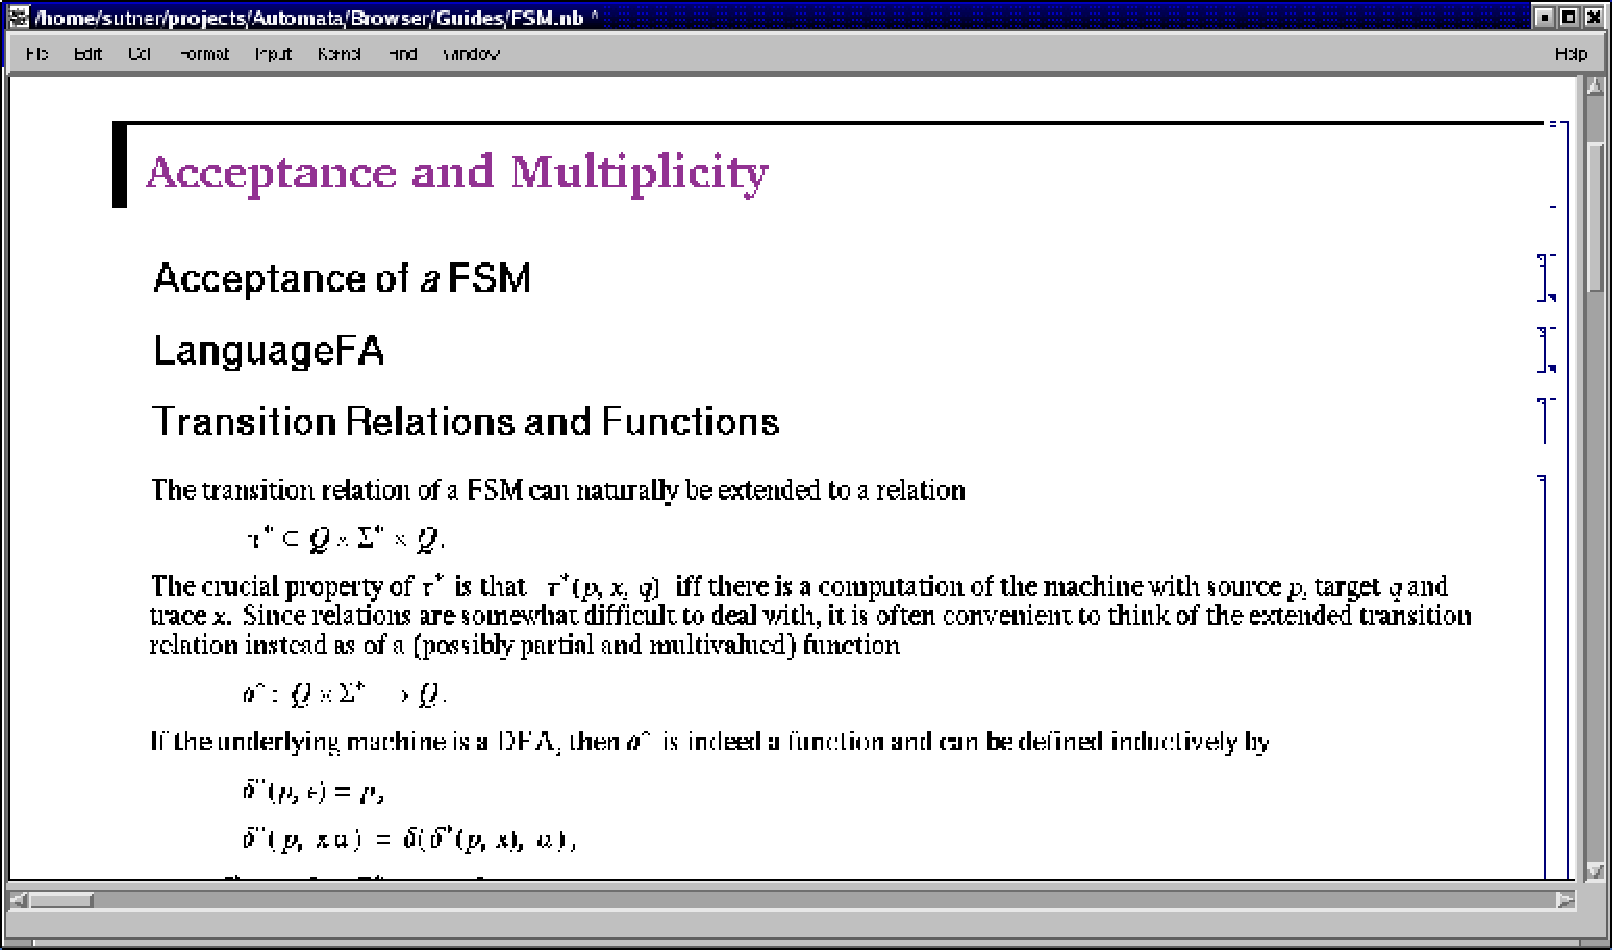
\includegraphics[width=10cm]{projects/mathematica/autosrc}
\end{myfig}

In order to facilitate the translation process it is advisable to front-load the
process: the author of the notebook is encouraged to use a special notebook
stylesheet, {\snippet{OMDocStyle.nb}}, that defines a number of syntactic categories
normally absent in a notebook.  These categories are implemented as a combination
of the cell types and cell labels.  As a typical example, consider a proof of some
assertion such as a theorem.  Ordinarily, a sequence of plain text cells would be
used to express a proof since none of the standard {\mathematica} stylesheets
provide a special proof style--though some have a theorem style.  The elements
defined in {\snippet{OMDocStyle.nb}} are easily accessible via pulldown menus or via
keyboard shortcuts in the notebook front end.  Moreover, the special styles are
color-coded in the notebook, so that it is easy for the author to see which
elements are present and which might be missing.


The conversion of mathematical expressions in the notebook is accomplished in a two-step
procedure.  First, we use the built-in {\mathematica} operation
{\snippet{ExpressionToSymbolicMathML}} that produces a symbolic expression representing a
MathML term that corresponds to the original notebook expression.  In a second,
post-processing step this expression is then transformed into an {\openmath} expression.
The post-processing relies heavily on the sophisticated pattern matching mechanism in
{\mathematica} and uses a special collection of rewrite rules.  The rules are based on
fairly simple-minded heuristics but do produce adequate results so long as the starting
expression is not too complicated.  As an example, consider the simple polynomial
expression $a x^2 + b x + c$ whose internal representation in {\mathematica} looks like so
(we assume here the expression appears inline within a block of text, the situation for an
input expression is entirely similar):
\begin{lstlisting}
Cell[ BoxData[FormBox[RowBox[{ 
      RowBox[{"a", " ", SuperscriptBox["x", "2"]}], "+", " ", 
      RowBox[{"b", " ", "x"}], " ", "+", " ", "c"}], 
        TraditionalForm]]]
\end{lstlisting}
The first conversion step produces the following {\mathematica} expression, 
shortened here to save space:
\begin{lstlisting}
XMLElement["math", 
  {"xmlns" ->"http://www.w3.org/1998/Math/MathML"}, 
  {XMLElement[ "apply", {}, {XMLElement["plus", {}, {}], 
   XMLElement[ "apply", {}, {XMLElement["times", {}, {}], 
     XMLElement["ci", {}, {"a"}], 
     XMLElement[ "apply", {}, {XMLElement["power", {}, {}], 
       XMLElement["ci", {}, {"x"}], 
       XMLElement["cn", {"type"->"integer"}, {"2"}]}]}], ...  }]}]
\end{lstlisting}
The post-processing finally yields the 
following expression, again shown only in part. 
\begin{lstlisting}
XMLElement["OMOBJ", {}, {XMLElement["OMA", {}, 
     {XMLElement["OMS", 
           {"cd"->"arith1", "name"->"plus"}, {}],
        XMLElement["OMA", {}, {XMLElement[ "OMS", 
           {"cd"->"arith1", "name"->"times"}, {}], 
        XMLElement["OMV", {"name"->"a"}, {}], 
        XMLElement["OMA", {}, {XMLElement["OMS", 
           {"cd"->"arith1", "name"->"power"}, {}], ...}]}]}]}]
\end{lstlisting}

The content dictionary was properly guessed in this instance.  Judging from the limited
experiments we have undertaken so far, it seems reasonable to expect that a fair amount of
the translation can be automated given that the field of discourse is limited, and that
the author is willing to customize the rewrite rules that control the post-processing
step.  Fortuitously, very little knowledge of {\mathematica} programming beyond some basic
syntax is necessary for the creation of these rules; mathematicians are likely to find
these rules fairly intuitive and natural.

At present, the conversion program is somewhat limited in its ability to deal with
arbitrarily structured notebooks.  It works well with a suite of notebooks developed
specifically for the {\snippet{OMDocStyle.nb}}, but requires modification for other types
of notebooks.  While it is not our goal to provide a truly general conversion tool with a
scope comparable to, say, the built-in conversion to MathML, some generalizations are
still needed at this point.

Another crucial issue is the extension of the rewrite rules used in the post-processing
step leading from MathML to {\openmath}.  No effort has been made so far to systematically
generate a set of rules suitable for a large class of documents.  At the very least, an
extension mechanism is needed that makes it easy for non-expert users to create the
necessary rule tables.

Lastly, it is desirable to create a {\mathematica} palette-based tool that focuses
more narrowly on the authoring and conversion of mathematical expressions only
rather than whole notebooks.  The generated raw {\openmath} expressions can be fed
directly into a low-level editor such as {\scsys{emacs}} using the special {\omdoc} mode
created as part of the {\ccaps} project, see elsewhere in this volume for a
description.

% LocalWords:  NotebookML evaluatable stylesheet OMDocStyle stylesheets BoxData
% LocalWords:  pulldown ExpressionToSymbolicMathML OpenMath FormBox RowBox nb
% LocalWords:  SuperscriptBox TraditionalForm XMLElement xmlns OMOBJ omdoc ci
% LocalWords:  arith CCaps thebib Sutner autosrc cn OMA cd OMV emacs

%%% Local Variables: 
%%% mode: latex
%%% TeX-master: "../../omdoc"
%%% End: 

\end{projectdescription}

\begin{projectdescription}
  %%%%%%%%%%%%%%%%%%%%%%%%%%%%%%%%%%%%%%%%%%%%%%%%%%%%%%%%%%%%%%%%%%%%%%%%%
% This file is part of the LaTeX sources of the OMDoc 1.3 specifiation
% Copyright (c) 2006 Christoph Lange
% This work is licensed by the Creative Commons Share-Alike license
% see http://creativecommons.org/licenses/by-sa/2.5/ for details
\svnInfo $Id: main.tex 8453 2009-08-04 09:58:26Z kohlhase $
\svnKeyword $HeadURL: https://svn.omdoc.org/repos/omdoc/branches/omdoc-1.3/doc/spec/projects/swim/main.tex $
%%%%%%%%%%%%%%%%%%%%%%%%%%%%%%%%%%%%%%%%%%%%%%%%%%%%%%%%%%%%%%%%%%%%%%%%%

\section{{\swim} -- An OMDoc-based Semantic Wiki}
\begin{project}{swim}{http://kwarc.eecs.iu-bremen.de/projects/swim}
\pauthors{Christoph Lange\and Michael Kohlhase}
\pinstitute{Computer Science, International University Bremen}
\end{project}

{\swim} is a semantic wiki for collaboratively building, editing and browsing a
mathematical knowledge base of {\omdoc} theories. Our long-term objective is to develop a
software that facilitates the creation of a shared, public collection of mathematical
knowledge and serves work groups of mathematicians as a tool for collaborative development
of new theories.  Even though the work reported here was initially motivated by solving
the MKM author's dilemma~\cite{KohKoh:cdad04}, we contend that the new application area
MKM can also contribute to the development of semantic wikis.

Technically, {\swim} is based on the semantic wiki engine
\scsys{IkeWiki}~\cite{schaffert06:ikewiki}, which was chosen because of its
modular design, its rich semantic web infrastructure, its user assistance for
annotations, and its orientation towards
learning~\cite{schaffert06:learning-with-semantic-wikis}.

\subsection{Semantic Wikis}

A wiki~\cite{LeuCun01:wikiway} is a web server
application that allows users to browse, create, and edit hyperlinked pages in a web
browser, usually using a simple text syntax.  In contrast to most content management
systems, wiki pages are accessible via an URL containing their title.  A new page can be
created by linking from an existent page to the page to be created.  This link will then
lead to an edit form.  Usually, anyone is allowed to edit pages on a wiki, but access can
be restricted.  Other characteristics of wikis include permanent storage of old page
versions (with facilities to display differences between two versions and to restore a
certain version), notification about recent changes, and full-text search.

Semantic
wikis~\cite{voelkel06:semanticwikistateoftheart,TolPas06:wikis-semantic-hypermedia}
enhance wikis by Semantic Web technologies, such as {\rdf}~\cite{LasSwi:rdf99} or
ontologies.  Usually one page represents one concept from a real-world domain, which has a
type, possibly some metadata, and typed links to other concepts.  For example, a link from
a wiki page about ``Life, the Universe and Everything'' to another page about Douglas
Adams could be typed as ``is author of''.  In terms of {\rdf}, this can be expressed by the
following subject--predicate--object triple,

\[
(\mbox{``Douglas Adams''},\;\mbox{isAuthorOf},\;\mbox{``Life, the Universe and
Everything''})
\]

where the \textit{isAuthorOf} relation would be defined in an ontology.  These links are
usually displayed in a navigation box next to the page contents. Semantic wikis only deal
with wiki text, not with mathematics, though some allow to embed mathematical formulae as
presentational-only {\TeX}.

{\swim} encourages users to collaborate: Non-mathematicians can collaborate in creating a
``Wikipedia of mathematics'' by compiling the knowledge available so far, while scientists
can collaboratively develop new theories.  Users get an immediate reward for many of their
contributions: Once they specify the type of a page or relations of one page to another,
this information will be displayed in a box of navigation links.  We intend to make the
data created in {\swim} usable for external services by offering an export facility for
{\omdoc} documents and by integrating them into {\swim}.  Mathematicians developing
theories will be assisted to retain an overview of theory dependencies in order not to
break them.  Social software services will further utilize the semantic information
available from the theories and from tracking the user interaction log (``Who did what on
which page when?'').  User feedback to pages can be extended to social bookmarking, which
is ``the practice of saving bookmarks [of Internet resources] to a public web site and
`tagging' them with keywords.''~\cite{lomas05:social-bookmarking} The more users tag a
certain resource, the higher a social bookmarking service will rank it.

The enhancements of the data model semantic wikis bring along --- compared to traditional
wikis --- are already present in the {\omdoc} format, so that an {\omdoc}-based wiki only
needs to operationalize their underlying meaning. For example, typed links, which are
implemented via an extension to the wiki syntax in \scsys{Semantic
  MediaWiki}~\cite{voelkel06:semanticwikipedia} or editable through a separate editor in
\scsys{IkeWiki}~\cite{schaffert06:ikewiki}, are implemented by means of the \texttt{for}
attribute to {\omdoc}'s elements (e.g.\ \texttt{<example for="\#id-of-assertion">}).
{\swim} makes them editable easily and visualizes them adequately.  A semantic wiki
targeted at mathematics must ensure that dependencies between concepts are preserved.
Results in this area will be interesting for non-mathematical semantic wikis as well,
especially when they support higher levels of formalization such as ontologies.

\subsection{Design of {\swim}}

\subsubsection{Concepts and Relations}

The smallest unit that can be displayed, edited, linked to, or archived in a wiki is a
page. In a semantic wiki, it usually describes one {\emph{concept}}, including its
properties and its relations to other concepts.  While standalone {\omdoc} documents can
contain more than one theory, is is important to keep pages small in a wiki to improve the
effectivity of usage.  Furthermore, usual semantic wikis only store and display metadata
and typed links per page; {\swim} does too.\footnote{Semantic information will only be
  considered on the theory and statement levels of {\omdoc} --- directly or through
  reasoning in the case of transitive closures ---, not on the object level.}  Users are
strongly encouraged to define at most one theory per wiki page and to roll out
non-constitutive statements (see {\mysecref{statements-constitutive}}) to separate pages,
referencing their context theory.  As constitutive statements cannot exist without an
enclosing theory, but as, on the other hand, we want each wiki page to form a valid
document, we introduced a new element {\element[ns-elt=swim]{page}}, which can be a child
of an {\element{omdoc}} element and which has the same content model as a
{\element{theory}} element --- in particular, it can hold several theory-constitutive
statements and connect them to their context theory.
\begin{wrapfigure}{r}{8cm}
  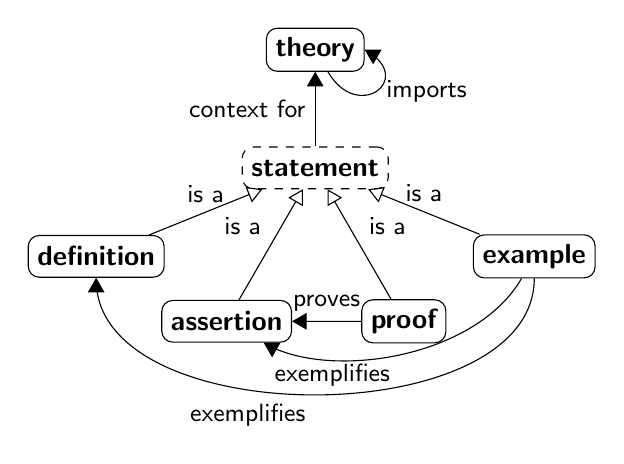
\begin{tikzpicture}[scale=1.5,thin,font=\sffamily,>=triangle 60]
    \tikzstyle{concept}=[font=\sffamily\bfseries,draw,minimum height=3.5ex,rounded corners]
    \tikzstyle{every path}=[font=\small\sffamily];
    \node[concept] (t) at (0,1) {theory};
    \node[concept,dashed] (s) at (0,0) {\itshape statement};
    \node[concept] (d) at +(-158:2.0cm) {definition};
    \begin{scope}[shift={(d)}]% control point for e->d
      \coordinate (da) at +(-90:1.5cm);% relative to s, not to a!
    \end{scope}
    \node[concept] (a) at +(-120:1.5cm) {assertion};
    \begin{scope}[shift={(a)}]% control point for e->a
      \coordinate (aa) at +(-30:1cm);% relative to s, not to a!
    \end{scope}
    \node[concept] (p) at +(-60:1.5cm) {proof};
    \node[concept] (e) at +(-22:2.0cm) {example};
    \draw[->] (t.-60) .. controls +(-60:0.5cm) and +(-30:0.5cm) .. node[right]
    {imports} (t.east);
    \draw[->] (s) -- node[left] {context for} (t);
    \draw[-open triangle 60] (d) -- node[above] {is a} (s);
    \draw[-open triangle 60] (a) -- node[above left] {is a} (s);
    \draw[-open triangle 60] (p) -- node[above right] {is a} (s);
    \draw[-open triangle 60] (e) -- node[above] {is a} (s);
    \draw[->] (p) -- node[above] {proves} (a);
    \draw[->] (e) ..
    controls +(-120:1cm)
    and (aa) ..
    node[below left] {exemplifies} (a);
    \draw[->] (e) ..
    controls +(-90:1.5cm)
    and (da) ..
    node[below left] {exemplifies} (d);
  \end{tikzpicture}
  \caption{Subset of {\omdoc}'s system ontology}\vspace*{-.5cm}
\end{wrapfigure}
{\omdoc}'s system ontology has been partly coded in OWL-DL and imported to the wiki's {\rdf}
store, which is implemented using the Jena Semantic Web Framework for
Java~\cite{URL:jena:web}. Theories as well as statements of any type form concepts, and
the most important relations between those concepts are extracted from the {\omdoc} pages
on saving and then stored as {\rdf} triples.  These relations include:
\begin{itemize}
\item The import relation between theories
\item The relation of a statement to its context theory
\item The relation of an example to the statement it exemplifies
\item The relation of a proof to the assertion it proves
\end{itemize}
It is planned to also take relations given by user interaction into consideration, such as
``Who edited which page when?'', and to combine ontology-defined relations and user
relations.  For example, a metric estimating the {\emph{degree of difficulty}} of a page,
calculated by counting the questions on the discussion page, could be implemented.
Furthermore, the user can specify taxonomic relations, which cannot be stated explicitly
in {\omdoc}, such as (``all differentiable functions are continuous''), as annotations in
an ontology language like {\rdf} Schema or {\owl}.

\subsubsection{User Interface and Interaction Model}

Pages can be rendered to XHTML plus presentational MathML using the transformations
described in {\mychapref{transform-xsl}}. There is also a browsable source code view, which is
useful for documents that are not written in textbook style.

Not only will the user be able to navigate along the dependency graph, she will also be
able to {\emph{interact}} with the system: she will be asked whether she wants to explore
the theories required as dependencies in further detail.

Suppose that the user is currently reading the page containing the theory {\snippet{ring}}
from the elementary algebra example from {\mychapref{dg-elal}}. In this case the wiki will
not only display navigation links to the direct dependencies {\snippet{group}} and
{\snippet{monoid}}, but it will also provide unobtrusive buttons that allow the user to
give one of the commands in {\myfigref{gui-showdeps}}. Not only the last case will be
recorded --- the others are interesting as well for \emph{social bookmarking}.  For
example, if many users requested a theory $t$ to be explained, the system could default to
display not only the direct dependencies but also the level-two dependencies, for it seems
that $t$ is too difficult for only being explained shallowly.

\begin{myfig}{gui-showdeps}{The command buttons to navigate along the dependencies}
  \begin{minipage}{8cm}
\begin{description}
\item[{\bf{No, thanks!}}] ``{\emph{I already know group and monoid.}}''
\item[{\bf{Explain}}] ``{\emph{Please show me group and monoid, I want to learn about
      ring's prerequisites.}}'' --- group and monoid will be displayed.
\item[{\bf{Explore}}] ``{\emph{Please show me {\emph{all}} prerequisites for ring.}}'' ---
  group, monoid, and semigroup, are opened in separate windows or serialized into one
  page.
\item[{\bf{Suspend}}] ``{\emph{I want to know about group and monoid, but only later.}}''
  --- {\swim} keeps a notice in the user's profile that she wants to read group and monoid
  sometime.  Reminder links to suspended theories are shown on a separate navigation bar.
\end{description}
\end{minipage}\quad
\begin{minipage}{2.5cm}
  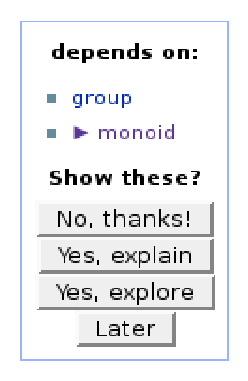
\includegraphics[width=2.5cm]{projects/swim/gui-showdeps}
\end{minipage}
\end{myfig}

\subsubsection{Further work}

Further work on {\swim} will concentrate on integrating a lightweight
management of change process.  Second, while the wiki is yet a user-friendly
\emph{browser}, there is still a demand for assisting users to \emph{edit}
{\omdoc}.  To this end, the {\qmath} preprocessor (see {\mysecref{qmath}}) will
be integrated into {\swim}.  Mathematical objects entered as {\qmath} will be
kept in this syntax for display in the edit form, but they will be converted to
{\omdoc} for rendering for presentation and when pages are exported to another
application.

%%% Local Variables: 
%%% mode: stex
%%% TeX-master: "../../omdoc"
%%% End: 

% LocalWords:  matwebsearch Ioan Sucan nC dx dy dt runningex XPointer ns attr
% LocalWords:  mq anyorder xmlns domainofapplication bvar ci cn eq OAI API da
% LocalWords:  Lange CPoint wikis dateness parseable isAuthorOf MediaWiki omdoc
% LocalWords:  aa wiki's Wiki wiki IkeWiki JA hypermedia elt semithick pres dg
% LocalWords:  elal gui showdeps qmath stex metadata wiki's scheint mir kein zu
% LocalWords:  Gegensatz sein

\end{projectdescription}

\begin{projectdescription}
  %%%%%%%%%%%%%%%%%%%%%%%%%%%%%%%%%%%%%%%%%%%%%%%%%%%%%%%%%%%%%%%%%%%%%%%%%
% This file is part of the LaTeX sources of the OMDoc 1.3 specifiation
% Copyright (c) 2006 Christoph Lange
% This work is licensed by the Creative Commons Share-Alike license
% see http://creativecommons.org/licenses/by-sa/2.5/ for details
\svnInfo $Id: main.tex 8453 2009-08-04 09:58:26Z kohlhase $
\svnKeyword $HeadURL: https://svn.omdoc.org/repos/omdoc/branches/omdoc-1.3/doc/spec/projects/swim/main.tex $
%%%%%%%%%%%%%%%%%%%%%%%%%%%%%%%%%%%%%%%%%%%%%%%%%%%%%%%%%%%%%%%%%%%%%%%%%

\section{{\swim} -- An OMDoc-based Semantic Wiki}
\begin{project}{swim}{http://kwarc.eecs.iu-bremen.de/projects/swim}
\pauthors{Christoph Lange\and Michael Kohlhase}
\pinstitute{Computer Science, International University Bremen}
\end{project}

{\swim} is a semantic wiki for collaboratively building, editing and browsing a
mathematical knowledge base of {\omdoc} theories. Our long-term objective is to develop a
software that facilitates the creation of a shared, public collection of mathematical
knowledge and serves work groups of mathematicians as a tool for collaborative development
of new theories.  Even though the work reported here was initially motivated by solving
the MKM author's dilemma~\cite{KohKoh:cdad04}, we contend that the new application area
MKM can also contribute to the development of semantic wikis.

Technically, {\swim} is based on the semantic wiki engine
\scsys{IkeWiki}~\cite{schaffert06:ikewiki}, which was chosen because of its
modular design, its rich semantic web infrastructure, its user assistance for
annotations, and its orientation towards
learning~\cite{schaffert06:learning-with-semantic-wikis}.

\subsection{Semantic Wikis}

A wiki~\cite{LeuCun01:wikiway} is a web server
application that allows users to browse, create, and edit hyperlinked pages in a web
browser, usually using a simple text syntax.  In contrast to most content management
systems, wiki pages are accessible via an URL containing their title.  A new page can be
created by linking from an existent page to the page to be created.  This link will then
lead to an edit form.  Usually, anyone is allowed to edit pages on a wiki, but access can
be restricted.  Other characteristics of wikis include permanent storage of old page
versions (with facilities to display differences between two versions and to restore a
certain version), notification about recent changes, and full-text search.

Semantic
wikis~\cite{voelkel06:semanticwikistateoftheart,TolPas06:wikis-semantic-hypermedia}
enhance wikis by Semantic Web technologies, such as {\rdf}~\cite{LasSwi:rdf99} or
ontologies.  Usually one page represents one concept from a real-world domain, which has a
type, possibly some metadata, and typed links to other concepts.  For example, a link from
a wiki page about ``Life, the Universe and Everything'' to another page about Douglas
Adams could be typed as ``is author of''.  In terms of {\rdf}, this can be expressed by the
following subject--predicate--object triple,

\[
(\mbox{``Douglas Adams''},\;\mbox{isAuthorOf},\;\mbox{``Life, the Universe and
Everything''})
\]

where the \textit{isAuthorOf} relation would be defined in an ontology.  These links are
usually displayed in a navigation box next to the page contents. Semantic wikis only deal
with wiki text, not with mathematics, though some allow to embed mathematical formulae as
presentational-only {\TeX}.

{\swim} encourages users to collaborate: Non-mathematicians can collaborate in creating a
``Wikipedia of mathematics'' by compiling the knowledge available so far, while scientists
can collaboratively develop new theories.  Users get an immediate reward for many of their
contributions: Once they specify the type of a page or relations of one page to another,
this information will be displayed in a box of navigation links.  We intend to make the
data created in {\swim} usable for external services by offering an export facility for
{\omdoc} documents and by integrating them into {\swim}.  Mathematicians developing
theories will be assisted to retain an overview of theory dependencies in order not to
break them.  Social software services will further utilize the semantic information
available from the theories and from tracking the user interaction log (``Who did what on
which page when?'').  User feedback to pages can be extended to social bookmarking, which
is ``the practice of saving bookmarks [of Internet resources] to a public web site and
`tagging' them with keywords.''~\cite{lomas05:social-bookmarking} The more users tag a
certain resource, the higher a social bookmarking service will rank it.

The enhancements of the data model semantic wikis bring along --- compared to traditional
wikis --- are already present in the {\omdoc} format, so that an {\omdoc}-based wiki only
needs to operationalize their underlying meaning. For example, typed links, which are
implemented via an extension to the wiki syntax in \scsys{Semantic
  MediaWiki}~\cite{voelkel06:semanticwikipedia} or editable through a separate editor in
\scsys{IkeWiki}~\cite{schaffert06:ikewiki}, are implemented by means of the \texttt{for}
attribute to {\omdoc}'s elements (e.g.\ \texttt{<example for="\#id-of-assertion">}).
{\swim} makes them editable easily and visualizes them adequately.  A semantic wiki
targeted at mathematics must ensure that dependencies between concepts are preserved.
Results in this area will be interesting for non-mathematical semantic wikis as well,
especially when they support higher levels of formalization such as ontologies.

\subsection{Design of {\swim}}

\subsubsection{Concepts and Relations}

The smallest unit that can be displayed, edited, linked to, or archived in a wiki is a
page. In a semantic wiki, it usually describes one {\emph{concept}}, including its
properties and its relations to other concepts.  While standalone {\omdoc} documents can
contain more than one theory, is is important to keep pages small in a wiki to improve the
effectivity of usage.  Furthermore, usual semantic wikis only store and display metadata
and typed links per page; {\swim} does too.\footnote{Semantic information will only be
  considered on the theory and statement levels of {\omdoc} --- directly or through
  reasoning in the case of transitive closures ---, not on the object level.}  Users are
strongly encouraged to define at most one theory per wiki page and to roll out
non-constitutive statements (see {\mysecref{statements-constitutive}}) to separate pages,
referencing their context theory.  As constitutive statements cannot exist without an
enclosing theory, but as, on the other hand, we want each wiki page to form a valid
document, we introduced a new element {\element[ns-elt=swim]{page}}, which can be a child
of an {\element{omdoc}} element and which has the same content model as a
{\element{theory}} element --- in particular, it can hold several theory-constitutive
statements and connect them to their context theory.
\begin{wrapfigure}{r}{8cm}
  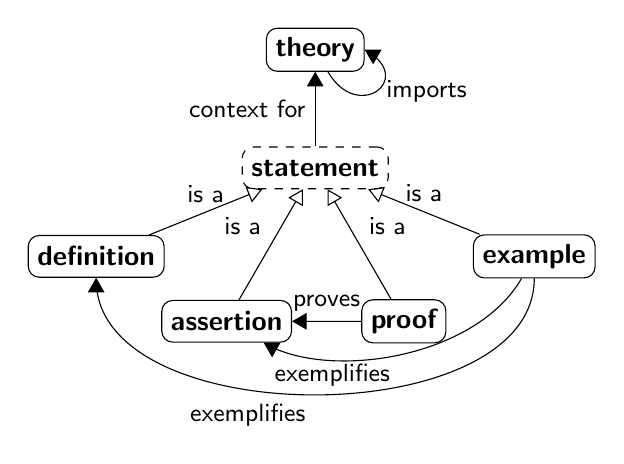
\begin{tikzpicture}[scale=1.5,thin,font=\sffamily,>=triangle 60]
    \tikzstyle{concept}=[font=\sffamily\bfseries,draw,minimum height=3.5ex,rounded corners]
    \tikzstyle{every path}=[font=\small\sffamily];
    \node[concept] (t) at (0,1) {theory};
    \node[concept,dashed] (s) at (0,0) {\itshape statement};
    \node[concept] (d) at +(-158:2.0cm) {definition};
    \begin{scope}[shift={(d)}]% control point for e->d
      \coordinate (da) at +(-90:1.5cm);% relative to s, not to a!
    \end{scope}
    \node[concept] (a) at +(-120:1.5cm) {assertion};
    \begin{scope}[shift={(a)}]% control point for e->a
      \coordinate (aa) at +(-30:1cm);% relative to s, not to a!
    \end{scope}
    \node[concept] (p) at +(-60:1.5cm) {proof};
    \node[concept] (e) at +(-22:2.0cm) {example};
    \draw[->] (t.-60) .. controls +(-60:0.5cm) and +(-30:0.5cm) .. node[right]
    {imports} (t.east);
    \draw[->] (s) -- node[left] {context for} (t);
    \draw[-open triangle 60] (d) -- node[above] {is a} (s);
    \draw[-open triangle 60] (a) -- node[above left] {is a} (s);
    \draw[-open triangle 60] (p) -- node[above right] {is a} (s);
    \draw[-open triangle 60] (e) -- node[above] {is a} (s);
    \draw[->] (p) -- node[above] {proves} (a);
    \draw[->] (e) ..
    controls +(-120:1cm)
    and (aa) ..
    node[below left] {exemplifies} (a);
    \draw[->] (e) ..
    controls +(-90:1.5cm)
    and (da) ..
    node[below left] {exemplifies} (d);
  \end{tikzpicture}
  \caption{Subset of {\omdoc}'s system ontology}\vspace*{-.5cm}
\end{wrapfigure}
{\omdoc}'s system ontology has been partly coded in OWL-DL and imported to the wiki's {\rdf}
store, which is implemented using the Jena Semantic Web Framework for
Java~\cite{URL:jena:web}. Theories as well as statements of any type form concepts, and
the most important relations between those concepts are extracted from the {\omdoc} pages
on saving and then stored as {\rdf} triples.  These relations include:
\begin{itemize}
\item The import relation between theories
\item The relation of a statement to its context theory
\item The relation of an example to the statement it exemplifies
\item The relation of a proof to the assertion it proves
\end{itemize}
It is planned to also take relations given by user interaction into consideration, such as
``Who edited which page when?'', and to combine ontology-defined relations and user
relations.  For example, a metric estimating the {\emph{degree of difficulty}} of a page,
calculated by counting the questions on the discussion page, could be implemented.
Furthermore, the user can specify taxonomic relations, which cannot be stated explicitly
in {\omdoc}, such as (``all differentiable functions are continuous''), as annotations in
an ontology language like {\rdf} Schema or {\owl}.

\subsubsection{User Interface and Interaction Model}

Pages can be rendered to XHTML plus presentational MathML using the transformations
described in {\mychapref{transform-xsl}}. There is also a browsable source code view, which is
useful for documents that are not written in textbook style.

Not only will the user be able to navigate along the dependency graph, she will also be
able to {\emph{interact}} with the system: she will be asked whether she wants to explore
the theories required as dependencies in further detail.

Suppose that the user is currently reading the page containing the theory {\snippet{ring}}
from the elementary algebra example from {\mychapref{dg-elal}}. In this case the wiki will
not only display navigation links to the direct dependencies {\snippet{group}} and
{\snippet{monoid}}, but it will also provide unobtrusive buttons that allow the user to
give one of the commands in {\myfigref{gui-showdeps}}. Not only the last case will be
recorded --- the others are interesting as well for \emph{social bookmarking}.  For
example, if many users requested a theory $t$ to be explained, the system could default to
display not only the direct dependencies but also the level-two dependencies, for it seems
that $t$ is too difficult for only being explained shallowly.

\begin{myfig}{gui-showdeps}{The command buttons to navigate along the dependencies}
  \begin{minipage}{8cm}
\begin{description}
\item[{\bf{No, thanks!}}] ``{\emph{I already know group and monoid.}}''
\item[{\bf{Explain}}] ``{\emph{Please show me group and monoid, I want to learn about
      ring's prerequisites.}}'' --- group and monoid will be displayed.
\item[{\bf{Explore}}] ``{\emph{Please show me {\emph{all}} prerequisites for ring.}}'' ---
  group, monoid, and semigroup, are opened in separate windows or serialized into one
  page.
\item[{\bf{Suspend}}] ``{\emph{I want to know about group and monoid, but only later.}}''
  --- {\swim} keeps a notice in the user's profile that she wants to read group and monoid
  sometime.  Reminder links to suspended theories are shown on a separate navigation bar.
\end{description}
\end{minipage}\quad
\begin{minipage}{2.5cm}
  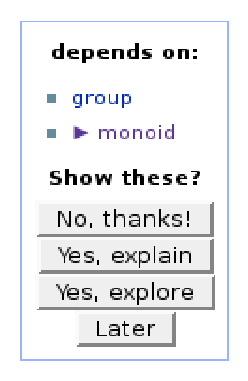
\includegraphics[width=2.5cm]{projects/swim/gui-showdeps}
\end{minipage}
\end{myfig}

\subsubsection{Further work}

Further work on {\swim} will concentrate on integrating a lightweight
management of change process.  Second, while the wiki is yet a user-friendly
\emph{browser}, there is still a demand for assisting users to \emph{edit}
{\omdoc}.  To this end, the {\qmath} preprocessor (see {\mysecref{qmath}}) will
be integrated into {\swim}.  Mathematical objects entered as {\qmath} will be
kept in this syntax for display in the edit form, but they will be converted to
{\omdoc} for rendering for presentation and when pages are exported to another
application.

%%% Local Variables: 
%%% mode: stex
%%% TeX-master: "../../omdoc"
%%% End: 

% LocalWords:  matwebsearch Ioan Sucan nC dx dy dt runningex XPointer ns attr
% LocalWords:  mq anyorder xmlns domainofapplication bvar ci cn eq OAI API da
% LocalWords:  Lange CPoint wikis dateness parseable isAuthorOf MediaWiki omdoc
% LocalWords:  aa wiki's Wiki wiki IkeWiki JA hypermedia elt semithick pres dg
% LocalWords:  elal gui showdeps qmath stex metadata wiki's scheint mir kein zu
% LocalWords:  Gegensatz sein

\end{projectdescription}

\begin{projectdescription}
  %%%%%%%%%%%%%%%%%%%%%%%%%%%%%%%%%%%%%%%%%%%%%%%%%%%%%%%%%%%%%%%%%%%%%%%%%
% This file is part of the LaTeX sources of the OMDoc 1.3 specifiation
% Copyright (c) 2006 Christoph Lange
% This work is licensed by the Creative Commons Share-Alike license
% see http://creativecommons.org/licenses/by-sa/2.5/ for details
\svnInfo $Id: main.tex 8453 2009-08-04 09:58:26Z kohlhase $
\svnKeyword $HeadURL: https://svn.omdoc.org/repos/omdoc/branches/omdoc-1.3/doc/spec/projects/swim/main.tex $
%%%%%%%%%%%%%%%%%%%%%%%%%%%%%%%%%%%%%%%%%%%%%%%%%%%%%%%%%%%%%%%%%%%%%%%%%

\section{{\swim} -- An OMDoc-based Semantic Wiki}
\begin{project}{swim}{http://kwarc.eecs.iu-bremen.de/projects/swim}
\pauthors{Christoph Lange\and Michael Kohlhase}
\pinstitute{Computer Science, International University Bremen}
\end{project}

{\swim} is a semantic wiki for collaboratively building, editing and browsing a
mathematical knowledge base of {\omdoc} theories. Our long-term objective is to develop a
software that facilitates the creation of a shared, public collection of mathematical
knowledge and serves work groups of mathematicians as a tool for collaborative development
of new theories.  Even though the work reported here was initially motivated by solving
the MKM author's dilemma~\cite{KohKoh:cdad04}, we contend that the new application area
MKM can also contribute to the development of semantic wikis.

Technically, {\swim} is based on the semantic wiki engine
\scsys{IkeWiki}~\cite{schaffert06:ikewiki}, which was chosen because of its
modular design, its rich semantic web infrastructure, its user assistance for
annotations, and its orientation towards
learning~\cite{schaffert06:learning-with-semantic-wikis}.

\subsection{Semantic Wikis}

A wiki~\cite{LeuCun01:wikiway} is a web server
application that allows users to browse, create, and edit hyperlinked pages in a web
browser, usually using a simple text syntax.  In contrast to most content management
systems, wiki pages are accessible via an URL containing their title.  A new page can be
created by linking from an existent page to the page to be created.  This link will then
lead to an edit form.  Usually, anyone is allowed to edit pages on a wiki, but access can
be restricted.  Other characteristics of wikis include permanent storage of old page
versions (with facilities to display differences between two versions and to restore a
certain version), notification about recent changes, and full-text search.

Semantic
wikis~\cite{voelkel06:semanticwikistateoftheart,TolPas06:wikis-semantic-hypermedia}
enhance wikis by Semantic Web technologies, such as {\rdf}~\cite{LasSwi:rdf99} or
ontologies.  Usually one page represents one concept from a real-world domain, which has a
type, possibly some metadata, and typed links to other concepts.  For example, a link from
a wiki page about ``Life, the Universe and Everything'' to another page about Douglas
Adams could be typed as ``is author of''.  In terms of {\rdf}, this can be expressed by the
following subject--predicate--object triple,

\[
(\mbox{``Douglas Adams''},\;\mbox{isAuthorOf},\;\mbox{``Life, the Universe and
Everything''})
\]

where the \textit{isAuthorOf} relation would be defined in an ontology.  These links are
usually displayed in a navigation box next to the page contents. Semantic wikis only deal
with wiki text, not with mathematics, though some allow to embed mathematical formulae as
presentational-only {\TeX}.

{\swim} encourages users to collaborate: Non-mathematicians can collaborate in creating a
``Wikipedia of mathematics'' by compiling the knowledge available so far, while scientists
can collaboratively develop new theories.  Users get an immediate reward for many of their
contributions: Once they specify the type of a page or relations of one page to another,
this information will be displayed in a box of navigation links.  We intend to make the
data created in {\swim} usable for external services by offering an export facility for
{\omdoc} documents and by integrating them into {\swim}.  Mathematicians developing
theories will be assisted to retain an overview of theory dependencies in order not to
break them.  Social software services will further utilize the semantic information
available from the theories and from tracking the user interaction log (``Who did what on
which page when?'').  User feedback to pages can be extended to social bookmarking, which
is ``the practice of saving bookmarks [of Internet resources] to a public web site and
`tagging' them with keywords.''~\cite{lomas05:social-bookmarking} The more users tag a
certain resource, the higher a social bookmarking service will rank it.

The enhancements of the data model semantic wikis bring along --- compared to traditional
wikis --- are already present in the {\omdoc} format, so that an {\omdoc}-based wiki only
needs to operationalize their underlying meaning. For example, typed links, which are
implemented via an extension to the wiki syntax in \scsys{Semantic
  MediaWiki}~\cite{voelkel06:semanticwikipedia} or editable through a separate editor in
\scsys{IkeWiki}~\cite{schaffert06:ikewiki}, are implemented by means of the \texttt{for}
attribute to {\omdoc}'s elements (e.g.\ \texttt{<example for="\#id-of-assertion">}).
{\swim} makes them editable easily and visualizes them adequately.  A semantic wiki
targeted at mathematics must ensure that dependencies between concepts are preserved.
Results in this area will be interesting for non-mathematical semantic wikis as well,
especially when they support higher levels of formalization such as ontologies.

\subsection{Design of {\swim}}

\subsubsection{Concepts and Relations}

The smallest unit that can be displayed, edited, linked to, or archived in a wiki is a
page. In a semantic wiki, it usually describes one {\emph{concept}}, including its
properties and its relations to other concepts.  While standalone {\omdoc} documents can
contain more than one theory, is is important to keep pages small in a wiki to improve the
effectivity of usage.  Furthermore, usual semantic wikis only store and display metadata
and typed links per page; {\swim} does too.\footnote{Semantic information will only be
  considered on the theory and statement levels of {\omdoc} --- directly or through
  reasoning in the case of transitive closures ---, not on the object level.}  Users are
strongly encouraged to define at most one theory per wiki page and to roll out
non-constitutive statements (see {\mysecref{statements-constitutive}}) to separate pages,
referencing their context theory.  As constitutive statements cannot exist without an
enclosing theory, but as, on the other hand, we want each wiki page to form a valid
document, we introduced a new element {\element[ns-elt=swim]{page}}, which can be a child
of an {\element{omdoc}} element and which has the same content model as a
{\element{theory}} element --- in particular, it can hold several theory-constitutive
statements and connect them to their context theory.
\begin{wrapfigure}{r}{8cm}
  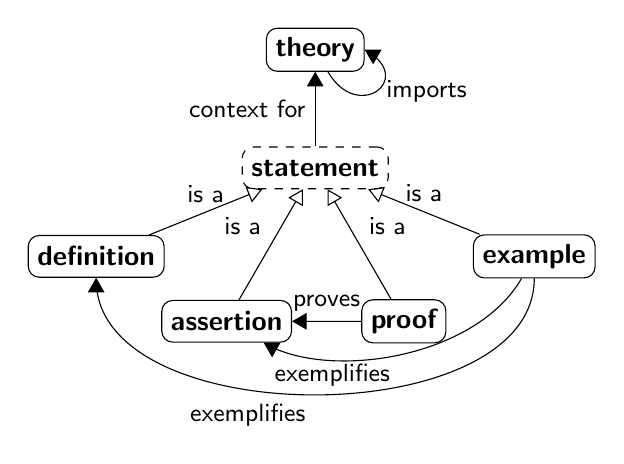
\begin{tikzpicture}[scale=1.5,thin,font=\sffamily,>=triangle 60]
    \tikzstyle{concept}=[font=\sffamily\bfseries,draw,minimum height=3.5ex,rounded corners]
    \tikzstyle{every path}=[font=\small\sffamily];
    \node[concept] (t) at (0,1) {theory};
    \node[concept,dashed] (s) at (0,0) {\itshape statement};
    \node[concept] (d) at +(-158:2.0cm) {definition};
    \begin{scope}[shift={(d)}]% control point for e->d
      \coordinate (da) at +(-90:1.5cm);% relative to s, not to a!
    \end{scope}
    \node[concept] (a) at +(-120:1.5cm) {assertion};
    \begin{scope}[shift={(a)}]% control point for e->a
      \coordinate (aa) at +(-30:1cm);% relative to s, not to a!
    \end{scope}
    \node[concept] (p) at +(-60:1.5cm) {proof};
    \node[concept] (e) at +(-22:2.0cm) {example};
    \draw[->] (t.-60) .. controls +(-60:0.5cm) and +(-30:0.5cm) .. node[right]
    {imports} (t.east);
    \draw[->] (s) -- node[left] {context for} (t);
    \draw[-open triangle 60] (d) -- node[above] {is a} (s);
    \draw[-open triangle 60] (a) -- node[above left] {is a} (s);
    \draw[-open triangle 60] (p) -- node[above right] {is a} (s);
    \draw[-open triangle 60] (e) -- node[above] {is a} (s);
    \draw[->] (p) -- node[above] {proves} (a);
    \draw[->] (e) ..
    controls +(-120:1cm)
    and (aa) ..
    node[below left] {exemplifies} (a);
    \draw[->] (e) ..
    controls +(-90:1.5cm)
    and (da) ..
    node[below left] {exemplifies} (d);
  \end{tikzpicture}
  \caption{Subset of {\omdoc}'s system ontology}\vspace*{-.5cm}
\end{wrapfigure}
{\omdoc}'s system ontology has been partly coded in OWL-DL and imported to the wiki's {\rdf}
store, which is implemented using the Jena Semantic Web Framework for
Java~\cite{URL:jena:web}. Theories as well as statements of any type form concepts, and
the most important relations between those concepts are extracted from the {\omdoc} pages
on saving and then stored as {\rdf} triples.  These relations include:
\begin{itemize}
\item The import relation between theories
\item The relation of a statement to its context theory
\item The relation of an example to the statement it exemplifies
\item The relation of a proof to the assertion it proves
\end{itemize}
It is planned to also take relations given by user interaction into consideration, such as
``Who edited which page when?'', and to combine ontology-defined relations and user
relations.  For example, a metric estimating the {\emph{degree of difficulty}} of a page,
calculated by counting the questions on the discussion page, could be implemented.
Furthermore, the user can specify taxonomic relations, which cannot be stated explicitly
in {\omdoc}, such as (``all differentiable functions are continuous''), as annotations in
an ontology language like {\rdf} Schema or {\owl}.

\subsubsection{User Interface and Interaction Model}

Pages can be rendered to XHTML plus presentational MathML using the transformations
described in {\mychapref{transform-xsl}}. There is also a browsable source code view, which is
useful for documents that are not written in textbook style.

Not only will the user be able to navigate along the dependency graph, she will also be
able to {\emph{interact}} with the system: she will be asked whether she wants to explore
the theories required as dependencies in further detail.

Suppose that the user is currently reading the page containing the theory {\snippet{ring}}
from the elementary algebra example from {\mychapref{dg-elal}}. In this case the wiki will
not only display navigation links to the direct dependencies {\snippet{group}} and
{\snippet{monoid}}, but it will also provide unobtrusive buttons that allow the user to
give one of the commands in {\myfigref{gui-showdeps}}. Not only the last case will be
recorded --- the others are interesting as well for \emph{social bookmarking}.  For
example, if many users requested a theory $t$ to be explained, the system could default to
display not only the direct dependencies but also the level-two dependencies, for it seems
that $t$ is too difficult for only being explained shallowly.

\begin{myfig}{gui-showdeps}{The command buttons to navigate along the dependencies}
  \begin{minipage}{8cm}
\begin{description}
\item[{\bf{No, thanks!}}] ``{\emph{I already know group and monoid.}}''
\item[{\bf{Explain}}] ``{\emph{Please show me group and monoid, I want to learn about
      ring's prerequisites.}}'' --- group and monoid will be displayed.
\item[{\bf{Explore}}] ``{\emph{Please show me {\emph{all}} prerequisites for ring.}}'' ---
  group, monoid, and semigroup, are opened in separate windows or serialized into one
  page.
\item[{\bf{Suspend}}] ``{\emph{I want to know about group and monoid, but only later.}}''
  --- {\swim} keeps a notice in the user's profile that she wants to read group and monoid
  sometime.  Reminder links to suspended theories are shown on a separate navigation bar.
\end{description}
\end{minipage}\quad
\begin{minipage}{2.5cm}
  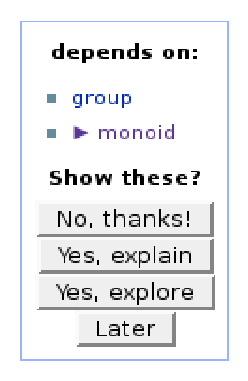
\includegraphics[width=2.5cm]{projects/swim/gui-showdeps}
\end{minipage}
\end{myfig}

\subsubsection{Further work}

Further work on {\swim} will concentrate on integrating a lightweight
management of change process.  Second, while the wiki is yet a user-friendly
\emph{browser}, there is still a demand for assisting users to \emph{edit}
{\omdoc}.  To this end, the {\qmath} preprocessor (see {\mysecref{qmath}}) will
be integrated into {\swim}.  Mathematical objects entered as {\qmath} will be
kept in this syntax for display in the edit form, but they will be converted to
{\omdoc} for rendering for presentation and when pages are exported to another
application.

%%% Local Variables: 
%%% mode: stex
%%% TeX-master: "../../omdoc"
%%% End: 

% LocalWords:  matwebsearch Ioan Sucan nC dx dy dt runningex XPointer ns attr
% LocalWords:  mq anyorder xmlns domainofapplication bvar ci cn eq OAI API da
% LocalWords:  Lange CPoint wikis dateness parseable isAuthorOf MediaWiki omdoc
% LocalWords:  aa wiki's Wiki wiki IkeWiki JA hypermedia elt semithick pres dg
% LocalWords:  elal gui showdeps qmath stex metadata wiki's scheint mir kein zu
% LocalWords:  Gegensatz sein

\end{projectdescription}

\end{tchapter}

%%% Local Variables: 
%%% mode: latex
%%% TeX-master: "omdoc"
%%% End: 

% LocalWords:  mtext activemath omdocmode cpoint nb frontend qmath maya mtxt
% LocalWords:  omdoctosys mathdox sentido FMP CMP omdoc mbase MMiSS verifun mkm
% LocalWords:  plugin texmacs stex


%%%%%%%%%%%%%%%%%%%%%%%%%%%%%%%%%%%%%%%%%%%%%%%%%%%%%%%%%%%%%%%%%%%%%%%%%
% This file is part of the LaTeX sources of the OMDoc 1.3 specification
% Copyright (c) 2006 Michael Kohlhase
% This work is licensed by the Creative Commons Share-Alike license
% see http://creativecommons.org/licenses/by-sa/2.5/ for details
%%%%%%%%%%%%%%%%%%%%%%%%%%%%%%%%%%%%%%%%%%%%%%%%%%%%%%%%%%%%%%%%%%%%%%%%%

\part{Appendix}\label{part:appendix}
  In this appendix, we document the changes of the OMDoc format over the versions,
  provide quick reference tables, and discuss the validation helps

%%% Local Variables: 
%%% mode: latex
%%% TeX-master: "omdoc"
%%% End: 
%%%% the appendix part
\begin{appendix}
%%%%%%%%%%%%%%%%%%%%%%%%%%%%%%%%%%%%%%%%%%%%%%%%%%%%%%%%%%%%%%%%%%%%%%%%%
% This file is part of the LaTeX sources of the OMDoc 1.3 specification
% Copyright (c) 2006 Michael Kohlhase
% This work is licensed by the Creative Commons Share-Alike license
% see http://creativecommons.org/licenses/by-sa/2.5/ for details
\svnInfo $Id: changes.tex 8685 2010-08-23 08:55:17Z kohlhase $
\svnKeyword $HeadURL: https://svn.omdoc.org/repos/omdoc/branches/omdoc-1.3/doc/spec/changes.tex $
%%%%%%%%%%%%%%%%%%%%%%%%%%%%%%%%%%%%%%%%%%%%%%%%%%%%%%%%%%%%%%%%%%%%%%%%%

\begin{tchapter}[id=changelog]{Changes to the specification}

After about 18 Months of development, Version 1.0 of the {\omdoc} format was released on
November $1^{st}$ 2000 to give users a stable interface to base their documents and
systems on. It was adopted by various projects in {\twintoo{automated}{deduction}},
{\twintoo{algebraic}{specification}}, and {\twintoo{computer-supported}{education}}. The
experience from these projects uncovered a multitude of small deficiencies and extension
possibilities of the format, that have been subsequently discussed in the {\omdoc}
{\indextoo{community}}.

{\omdocv{1.1}} was released on December $29^{th}$ 2001 as an attempt to roll the
uncontroversial and non-disruptive part of the extensions and corrections into a
consistent language format. The changes to version 1.0 were largely conservative,
adding optional attributes or child elements. Nevertheless, some non-conservative
changes were introduced, but only to less used parts of the format or in order to
remedy design flaws and inconsistencies of version 1.0.

{\omdocv{1.3}} is the mature version in the {\omdocv{1}} series of specifications. It
contains almost no large-scale changes to the document format, except that {\cmathml} is
now allowed as a representation for mathematical objects. But many of the representational
features have been fine-tuned and brought up to date with the maturing {\xml} technology
(e.g. {\snippet{ID}}\twin{type}{ID} attributes now follow the XML ID
specification~\cite{XML:id05}, and the Dublin Core elements follow the official
syntax~\cite{DCMI:dmt03}). The main development is that the {\omdoc} specification, the
DTD, and schema are split into a system of interdependent modules that support independent
development of certain language aspects and simpler specification and deployment of
sub-languages.  {\vomdoc{1.3}} freezes the development so that version 2 can be started
off on the modules.

In the following, we will keep a log on the changes that have occurred in the
released versions of the {\omdoc} format.  We will briefly tabulate the changes by
element name. For the state of an element we will use the shorthands ``dep'' for
{\indextoo{deprecated}} (i.e. the element is no longer in use in the new {\omdoc}
version), ``cha'' for {\indextoo{changed}}, if the element is re-structured (i.e.
some additions and losses), ``new'' if did not exist in the old {\omdoc} version,
``lib'', if it was liberalized (e.g. an attribute was made optional) and finally
``aug'' for {\indextoo{augmented}}, i.e. if it has obtained additional children or
attributes in the new {\omdoc} version.

All changes will be relative to the previous version, starting out with OMDoc 1.0.

%%%%%%%%%%%%%%%%%%%%%%%%%%%%%%%%%%%%%%%%%%%%%%%%%%%%%%%%%%%%%%%%%%%%%%%%%
% This file is part of the LaTeX sources of the OMDoc 1.3 specification
% Copyright (c) 2016 Michael Kohlhase.
% Source at https://github.com/KWARC/OMDoc/tree/master/doc/spec
% This work is licensed by the Creative Commons Share-Alike license
% see http://creativecommons.org/licenses/by-sa/2.5/ for details
%%%%%%%%%%%%%%%%%%%%%%%%%%%%%%%%%%%%%%%%%%%%%%%%%%%%%%%%%%%%%%%%%%%%%%%%%

\begin{tsection}[id=changes1.3]{Changes from 1.2 to 1.3}

  The main change from {\omdocv{1.2}} to {\omdocv{1.3}} is the use of the new notation
  framework described in {\mychapref{pres}}. It completely replaces the presentation
  archicture of {\omdocv{1.2}}.

  The other large change is to use the new namespace \url{http://omdoc.org/ns} that will
  also be used in {\omdocv{1.2}}

\begin{center}\footnotesize
\begin{longtable}{|l|c|p{6cm}|l|}\hline
  element & state & comments & cf.\\\hline\hline 
{\element{dd}}           & cha
     & description items now allow block content as in XHTML
     & \mysecref{mtxt} \\\hline
{\element{bibliography}}           & new
     & generates the references
     & \mysecref{frontbackmatter} \\\hline
{\element{citation}}           & new
     & marks up a citation
     & \mysecref{mtxt} \\\hline
{\element{index}}           & new
     & generates the index
     & \mysecref{frontbackmatter} \\\hline
{\element{li}}           & cha
     & list items now allow block content as in XHTML
     & \mysecref{mtxt} \\\hline
{\element{metadata}}        & cha
     & the optional attribute {\oldattribute{inherits}{metadata}{1.2}} dropped, it was never
     sufficiently defined.
     & \mysecref{metadata}\\\hline
{\oldelement{presentation}{1.2}}           & del
     & replaced by the {\element{notation}} element. 
     & \mychapref{pres} \\\hline
{\oldelement{style}{1.2}}           & del
     & obsolete, since it was never used.
     & \\\hline
{\element{tableofcontents}}           & new
     & generates the tableofcontents
     & \mysecref{frontbackmatter} \\\hline
{\oldelement{tgroup}{1.2}}           & del
     & replaced by the {\element{omgroup}} element, it turns out that with RelaxNG we can
     do the necessary validation of theory content after all. 
     & \mychapref{statements} \\\hline
{\element{uses}}           & new
     & opens a CD catalog.
     & \mychapref{mtext} \\\hline
\end{longtable}
\end{center}
\end{tsection}

%%% Local Variables: 
%%% mode: stex
%%% TeX-master: "omdoc"
%%% End: 

%%%%%%%%%%%%%%%%%%%%%%%%%%%%%%%%%%%%%%%%%%%%%%%%%%%%%%%%%%%%%%%%%%%%%%%%%
% This file is part of the LaTeX sources of the OMDoc 1.3 specification
% Copyright (c) 2016 Michael Kohlhase.
% Source at https://github.com/KWARC/OMDoc/tree/master/doc/spec
% This work is licensed by the Creative Commons Share-Alike license
% see http://creativecommons.org/licenses/by-sa/2.5/ for details
%%%%%%%%%%%%%%%%%%%%%%%%%%%%%%%%%%%%%%%%%%%%%%%%%%%%%%%%%%%%%%%%%%%%%%%%%

\begin{tsection}[id=changes1.2]{Changes from 1.1 to 1.2}

  Most of the changes in version 1.2 are motivated by modularization. The goal was
  to modularize the specification so that it can be used as a DTD module, and that
  restricted sub-languages of {\omdoc} can be identified. 
  
  Perhaps the most disruptive change is in the presentation/style apparatus: In version
  1.1, {\omdoc} used the {\attributeshort{style}} attribute for all elements that have an
  {\attributeshort{id}} attribute to specify generic style classes for the {\omdoc}
  elements.  This was based on a misunderstanding of the {\xml} {\twintoo{cascading}{style
      sheet}} ({\css}) mechanism~\cite{BosHak:css98}, which uses the
  {\attributeshort{class}} attribute to specify this information and uses the
  {\attributeshort{style}} attribute to specify {\css} directives\twin{CSS}{directive}
  that override the class information.  This error in {\vomdoc{1.1}} so severely limits
  the usefulness for styling that we rename the {\vomdoc{1.1}}
  {\attributeshortcomment{style}{meaning changed in 1.2}} attribute to
  {\attributeshort{class}}, even though it breaks 1.1-compatible
  implementations. Concretely, the {\vomdoc{1.2}} {\attributeshort{class}} attribute takes
  the role of the {\vomdoc{1.1}} {\attributeshortcomment{style}{meaning changed in
      1.2}}. and the {\vomdoc{1.2}} {\attributeshortcomment{style}{new meaning
      1.2}}\label{style/class-comment} takes {\css} directives\twin{CSS}{directive}.

  Furthermore, all {\attributeshort[ns-attr=xml]{id}} on non-constitutive (see
  {\mysecref{statements-constitutive}}) elements in {\omdoc} were made optional.
  
  {\vomdoc{1.1}} files can be upgraded to version 1.2 with the {\xslt} style sheet
    \url{https://svn.omdoc.org/repos/omdoc/branches/omdoc-1.2/xsl/omdoc1.1adapt1.2.xsl}.

\begin{center}\footnotesize
\begin{longtable}{|l|c|p{6cm}|l|}\hline
  element & state & comments & cf.\\\hline\hline 
{\element{alternative}} & aug
     &  This element can now have {\attribute{theory}{alternative}},
    {\attribute{generated-from}{alternative}}, and
    {\attribute{generated-via}{alternative}} attributes.
     & \pageref{eldef:alternative}\\\hline
{\element{argument}} & cha
     &  The {\oldattribute{sort}{argument}{1.2}} has been replaced by a {\element{type}}
     child, so that higher-order sorts can be specified. 
     & \pageref{eldef:argument}\\\hline
{\element{assertion}} & aug 
  & the {\element{assertion}} element now has an optional {\attribute{for}{assertion}}
     attribute. Furthermore, an optional attribute {\attribute{generated-via}{assertion}}
     has been added to allow generation via a theory morphism. Finally, two new attributes
     {\attribute{status}{assertion}} and {\attribute{just-by}{assertion}} have been added
     to mark up the deductive status of the assertion. 
  & \pageref{eldef:assertion}\\\hline 
{\element{assumption}} & cha
     &  This element can now have an attribute {\attribute{inductive}{assumption}} for
     inductive assumptions. The natural langauge description in the optional
     {\element{CMP}} element  is no longer allowed, use a {\element{phrase}} element in
     a {\element{CMP}} that is a sibling to the {\element{FMP}} instead.
     & \pageref{eldef:alternative}\\\hline
{\element{adt}} & aug 
  & the {\element{adt}} loses the {\element{CMP}} and {\oldelement{commonname}{1.2}}
  children, use the Dublin Core metadata elements {\element[ns-elt=dc]{description}} and
  {\element[ns-elt=dc]{subject}} instead. The {\attribute{type}{adt}} attribute is now on
  the {\element{sortdef}} element. Furthermore, an optionala
     attribute {\attribute{generated-via}{adt}} 
     has been added to allow generation via a theory morphism. Finally, an attribute
     {\attribute{parameters}{adt}} has been added to allow for parametric ADTs. 
  & \pageref{eldef:adt}\\\hline 
{\element{answer}} & cha
  & the {\element{answer}} element does not allow {\element{symbol}} children
  any more, if these are needed, the exercise should have its own theory.
  & \pageref{eldef:answer}\\\hline 
{\element{attribute}} & aug
  & the {\element{attribute}} element now has a optional {\attribute{ns}{attribute}}
  attribute for the namespace URI of the generated attribute node and an attribute
  {\attribute{select}{attribute}} for an {\xpath} expression that specifies the value of
  the generated attribute.
  & \pageref{eldef:attribute}\\\hline 
{\element{axiom}} & aug 
  & the {\element{axiom}} element now has an optional {\attribute{for}{axiom}}
     attribute which can point to a list of symbols. Furthermore, an optional
     attribute {\attribute{generated-via}{assertion}} 
     has been added to allow generation via a theory morphism and an attribute
     {\attribute{type}{axiom}} is now also allowed. 
  & \pageref{eldef:axiom}\\\hline
{\element{axiom-inclusion}} & lib 
  & the {\element{axiom-inclusion}} element can now contain multiple
    {\element{path-just}} children to record multiple justifications.  
    Furthermore, it can now have {\attribute{theory}{axiom-inclusion}},
    {\attribute{generated-from}{axiom-inclusion}}, and
    {\attribute{generated-via}{axiom-inclusion}} attributes.
    New optional attributes {\attribute{conservativity}{axiom-inclusion}} and
    {\attribute{conservativity-just}{axiom-inclusion}} for stating and justifying
    conservativity. 
  & \pageref{eldef:axiom-inclusion}\\\hline
{\oldelement{catalogue}{1.1}} & dep
  & the catalogue mechanism has been eliminated.
  & \\\hline 
{\element{choice}} & cha
  & the {\element{choice}} element does not allow {\element{symbol}} children
  any more, if these are needed, the exercise should have its own theory
  & \pageref{eldef:choice}\\\hline 
{\element{code}}        & cha 
     & Attributes {\oldattribute{classid}{code}{1.2}} and
       {\oldattribute{codebase}{code}{1.2}} are deprecated.  The attributes
       {\attribute{pto}{data}}  and {\attribute{pto-version}{data}} have moved to
       the {\element{data}} element. The attribute
       {\oldattribute{type}{code}{1.1}} has been removed and
    optional attributes {\attribute{theory}{private}},
    {\attribute{generated-from}{private}}, and
    {\attribute{generated-via}{private}} have been added.     
  & \pageref{eldef:code}\\\hline
{\oldelement{commonname}{1.2}}        & dep
     & This element is deprecated in favor of a
     {\element{metadata}}/{\element[ns-elt=dc]{subject}} element.
     & \\\hline
{\element{conclusion}} & cha
     & The natural langauge description in the optional
     {\element{CMP}} element  is no longer allowed, use a {\element{phrase}} element in
     a {\element{CMP}} that is a sibling to the {\element{FMP}} instead.
     & \pageref{eldef:conclusion}\\\hline
{\element{constructor}} & cha 
  & The {\attribute{role}{constructor}} attribute is now fixed to
    {\attval{object}{type}{constructor}}.   The
    {\oldelement{commonname}{1.2}} child has been replaced by an initial
    {\element{metadata}} element.
  & \pageref{eldef:constructor} \\\hline
{\element{data}}           & aug
     & new optional attributes {\attribute{original}{data}} to specify whether the
     external resource referenced by the  {\attribute{href}{data}} attribute
     (value {\attval{external}{original}{data}}) or the 
     {\element{data}} content is the original (value
     {\attval{local}{original}{data}}).  The  {\element{data}} element has
     acquired attributes {\attribute{pto}{data}}
    and {\attribute{pto-version}{data}}  from the {\element{code}} and
    {\element{private}} elements. 
     & \pageref{eldef:data}\\\hline
{\element[ns-elt=dc]{*}}                 & aug 
     & All Dublin Core tags have been lowercased  to synchronize with the tag
       syntax recommended by the Dublin Core Initiative. The tags were capitalized
       in {\omdoc}1.1. Furthermore, {\element[ns-elt=dc]{contributor}}, {\element[ns-elt=dc]{creator}},
       {\element[ns-elt=dc]{publisher}} have  
       received an optional {\attributeshortcomment{xml:id}{on Dublin Core elements}} 
       attribute, so that they can be cross-referenced by the new 
       {\attribute[ns-elt=dc]{who}{date}} of the {\element[ns-elt=dc]{date}} element.
     & \pageref{eldef:dc:title}\\\hline
{\element{decomposition}} & aug 
  & The {\attribute{for}{decomposition}} attribute
    is now optional, it need not be given, if the element is a child of a
    {\element{theory-inclusion}} element. Furthermore, it can now have a
    {\attribute{theory}{decomposition}}, 
    {\attribute{generated-from}{decomposition}}, and
    {\attribute{generated-via}{decomposition}} attributes.
  & \pageref{eldef:decomposition} \\\hline
{\element[ns-elt=dc]{description}} & aug
  & The {\element[ns-elt=dc]{description}} can now have the optional
    {\attribute[ns-attr=xml]{id}{description}}, and {\css} attributes\twin{CSS}{attribute}
  & \pageref{eldef:dc:description} \\\hline
{\element{definition}} & aug
  & The {\element{definition}} element can now have the type
  {\attval{pattern}{type}{definition}} for pattern-defined functions. This is a
  degenerate case of the type {\attval{inductive}{type}{definition}}. Furthermore, an optional
     attribute {\attribute{generated-via}{assertion}} 
     has been added to allow generation via a theory morphism.
  & \pageref{eldef:definition} \\\hline
{\element{effect}} & aug
  & allows an optional  {\attribute[ns-attr=xml]{id}{effect}} attribute
  & \pageref{eldef:effect}\\\hline
{\element{example}} & aug
  & The {\element{example}} element now has the optional {\attribute{theory}{example}}
  attribute that specifies the home theory.
     Furthermore, it can now have attributes {\attribute{theory}{example}},
    {\attribute{generated-from}{example}}, and
    {\attribute{generated-via}{example}}.
  & \pageref{eldef:example} \\\hline
{\element{exercise}} & cha
  & the {\element{exercise}} element does not allow {\element{symbol}} children
  any more, if these are needed, the exercise should have its own theory.
   Furthermore, it can now have a {\attribute{theory}{exercise}},
    {\attribute{generated-from}{exercise}}, and
    {\attribute{generated-via}{exercise}} attributes.
  & \pageref{eldef:exercise}\\\hline 
{\oldelement{extradata}{1.2}} & cha
  & The content of the old {\oldelement{extradata}{1.2}} element can now be directly in
  the {\element{metadata}}/{\element[ns-elt=dc]{subject}} element.
  & \\\hline 
{\element{element}} & aug
  & The {\element{element}} element now allows the {\element{map}} and
  {\element{separator}} elements in the body. Furthermore, it carries the optional
  attributes {\attribute{crid}{element}} for parallel markup, {\attribute{cr}{element}}
  for cross-references, and {\attribute{ns}{element}} for specifying the namespace.
  & \pageref{eldef:element} \\\hline
{\element{hint}} & aug 
  & the {\element{hint}} element can now appear on top-level and
    has a {\attribute{for}{hint}} attribute.  It does not allow {\element{symbol}} children
    any more, if these are needed, the exercise should have its own theory.
    Furthermore, the {\element{exercise}} can now have a {\attribute{theory}{hint}},
    {\attribute{generated-from}{hint}}, and {\attribute{generated-via}{hint}} attributes.
  & \pageref{eldef:hint}\\\hline
{\element{hypothesis}} & cha
  & the {\oldattribute{discharged-in}{hypothesis}{1.2}} attribute has been
  eliminated. Scoping is now specified in terms of the enclosing {\element{proof}}
  element. Furthermore, the {\element{symbol}} child is no longer allowed inside
  the element. A sibling {\element{symbol}} should be used. 
  & \pageref{eldef:hypothesis}\\\hline
{\element{inclusion}} & aug
  & allows optional attributes {\attribute[ns-attr=xml]{id}{inclusion}}, 
     {\attribute{conservativity}{inclusion}}, and
    {\attribute{conservativity-just}{inclusion}} for stating and justifying
    conservativity. 
  & \pageref{eldef:inclusion}\\\hline
{\element{imports}} & lib
  & the {\attribute[ns-attr=xml]{id}{imports}} is now optional.
    New optional attributes {\attribute{conservativity}{imports}} and
    {\attribute{conservativity-just}{imports}} for stating and justifying
    conservativity. 
  & \pageref{eldef:imports}\\\hline
{\element{input}} & aug
  & allows an optional  {\attribute[ns-attr=xml]{id}{input}} attribute
  & \pageref{eldef:input}\\\hline
{\element{legacy}} & new 
  & An element for encapsulating legacy mathematics, can
    be used wherever {\element[ns-elt=m]{math}} and {\element[ns-elt=om]{OMOBJ}} are allowed.  
  & \pageref{eldef:legacy}\\\hline
{\oldelement{loc}{1.1}} & dep
  & The catalogue mechanism has been eliminated.
  & \\\hline
{\element[ns-elt=m]{math}} & new 
  & {\cmathml} is now allowed wherever {\openmath} objects were allowed before.  
  & \pageref{eldef:m:math}\\\hline
{\element{map}} & new 
  & this element allows to map its style directives over a list of e.g. arguments
  & \pageref{eldef:map}\\\hline
{\element{mc}} & aug 
  & the {\element{mc}} element can now have a {\attribute{for}{mc}}
  attribute. It does not allow {\element{symbol}} children
  any more, if these are needed, the dominating {\element{exercise}} element should have
  its own theory. Furthermore, the {\element{mc}} element can now have a
  {\attribute{theory}{mc}},  {\attribute{generated-from}{mc}}, and
  {\attribute{generated-via}{mc}} attributes.
  & \pageref{eldef:mc}\\\hline
{\element{measure}} & aug
  & allows an optional  {\attribute[ns-attr=xml]{id}{measure}} attribute
  & \pageref{eldef:measure}\\\hline
{\oldelement{metacomment}{1.2}} & dep
  & This element is superseded by the {\element{omtext}} element. 
  & \pageref{eldef:omtext}\\\hline
{\element{morphism}} & aug 
  & The {\element{morphism}}  element now carries the optional  attributes
  {\attribute{consistency}{morphism}},  {\attribute{exhaustivity}{morphism}}, 
  {\attribute{hiding}{morphism}}, and {\attribute{type}{morphism}}. Furthermore the  content model 
  allows optional elements {\element{measure}} and {\element{ordering}}  after the
  {\element{requation}}  children to specify termination information like in
  {\element{definition}}. 
  & \pageref{eldef:metadata}\\\hline
{\element{obligation}} & aug
  & allows an optional  {\attribute[ns-attr=xml]{id}{obligation}} attribute
  & \pageref{eldef:obligation}\\\hline
{\element{omdoc}} & aug 
  & This element can now have a {\attribute{theory}{omdoc}},
    {\attribute{generated-from}{omdoc}}, and
    {\attribute{generated-via}{omdoc}} attributes.
  & \pageref{eldef:omdoc}\\\hline
{\element{omgroup}} & cha 
  & The values {\oldattval{dataset}{type}{omgroup}{1.2}} and
    {\oldattval{labeled-dataset}{type}{omgroup}{1.2}} are deprecated in {\vomdoc{1.2}},
    since we provide tables in module {\RTmodule{spec}}; see {\mysecref{rt}} for
    details.  Furthermore, the element can now have the attributes,
    {\attribute{modules}{omgroup}}, {\attribute{theory}{omgroup}},
    {\attribute{generated-from}{omgroup}}, and
    {\attribute{generated-via}{omgroup}}.
  & \pageref{eldef:omgroup}\\\hline
{\element{omlet}} & cha
  & {\element{omlet}} can no longer occur at top-level (it just does not make
    sense).  The data model for this element has been totally reworked, inspired
    by  the {\element[ns-elt=xhtml]{object}} element. 
  & \pageref{eldef:omlet}\\\hline
{\element{omstyle}} & aug 
  & This element can now have {\attribute{generated-from}{omstyle}}, and
    {\attribute{generated-via}{omstyle}} attributes. New attribute
    {\attribute{xref}{omstyle, presentation}} that allows to inherit the information 
    from another {\element{omstyle}} element. 
  & \pageref{eldef:omstyle}\\\hline
{\element[ns-elt=om]{*}} & aug 
  & with {\openmath}2, the {\openmath} elements carry an optional {\attribute[ns-elt=om]{id}{*}} 
    attribute for structure sharing via the {\element[ns-elt=om]{OMR}} element. Furthermore, in
    {\omdoc}, they carry
    {\attribute[ns-elt=om]{cref}{*}} attributes for parallel markup with {\indextoo{cross-reference}s}.  
  & \pageref{eldef:om:OMA}\\\hline
{\element[ns-elt=om]{OMFOREIGN}} & new & The {\element[ns-elt=om]{OMFOREIGN}}
    element can be used to encapsulate arbitrary {\xml} data in {\openmath}
    attributions.  
  & \pageref{eldef:om:OMFOREIGN}\\\hline
{\element[ns-elt=om]{OMR}} & new 
  & In the {\openmath}2 standard, this element is the main
    vehicle of the structure sharing representation.  
  & \pageref{eldef:om:OMR}\\\hline
  {\element{omtext}} & aug 
  & the {\attribute{type}{omtext}} attribute can now also have the
    values {\attval{axiom}{type}{omtext}}, {\attval{definition}{type}{omtext}},
    {\attval{theorem}{type}{omtext}}, {\attval{proposition}{type}{omtext}},
    {\attval{lemma}{type}{omtext}}, {\attval{corollary}{type}{omtext}},
    {\attval{postulate}{type}{omtext}}, {\attval{conjecture}{type}{omtext}},
    {\attval{false-conjecture}{type}{omtext}}, {\attval{obligation}{type}{omtext}},
    {\attval{assumption}{type}{assertion}}, and {\attval{formula}{type}{omtext}}.  

    Furthermore, {\element{omtext}} can now have {\attribute{theory}{omtext}},
    {\attribute{generated-from}{omtext}}, and
    {\attribute{generated-via}{omtext}} and {\attribute{verbalizes}{omtext}} attributes.
  & \pageref{eldef:omtext}\\\hline
{\element{ordering}} & aug
  & Now allows the optional  {\attribute[ns-attr=xml]{id}{ordering}} and
  {\attribute{terminating}{ordering}} attributes. The latter points to a termination
  assertion. 
  & \pageref{eldef:ordering}\\\hline
{\element{output}} & aug
  & allows an optional  {\attribute[ns-attr=xml]{id}{input}} attribute
  & \pageref{eldef:output}\\\hline
{\oldelement{pattern}{1.2}} & aug
  & this element is no longer used, the pattern of a recursive equation is determined by
  the position as the first child.
  & \\\hline
{\element{path-just}} & aug 
  & The element can now appear as a top-level element,
    if it does, the attribute {\attribute{for}{path-just}} must point to the
    {\element{axiom-inclusion}} element it justifies.  It also now
   allows an optional  {\attribute[ns-attr=xml]{id}{input}} attribute
  & \pageref{eldef:path-just}\\\hline
{\element{phrase}}           & new
     & used to mark up phrases in {\element{CMP}s} and supply them with
       identifiers and links to context that can be 
       used for presentation and referencing.
     & \pageref{eldef:phrase}\\\hline
{\element{presentation}} & cha
  & The {\oldattribute{theory}{presentation}{1.2}} is not allowed any more, to refer to a symbol
    outside its theory use its {\attribute[ns-attr=xml]{id}{symbol}} attribute. 
    The element now also allows a mutilingual {\element{CMP}} group,
    so that it can be used as a notation definition element in mathematical vernacular. 
  & \pageref{eldef:presentation} \\\hline
{\element{private}} & cha
  & The {\oldattribute{replaces}{private}{1.2}} attribute is now called
    {\attribute{reformulates}{private}}. The attributes {\attribute{pto}{data}}
    and {\attribute{pto-version}{data}} have moved to the {\element{data}}
    element.  The attribute {\oldattribute{type}{code}{1.1}} has been removed and
    optional attributes {\attribute{theory}{private}},
    {\attribute{generated-from}{private}}, and
    {\attribute{generated-via}{private}} have been added.
  & \pageref{eldef:private} \\\hline
{\element{proof}} & lib 
  & The {\attribute{for}{proof}} attribute is now optional to allow for proofs as
    objects of mathematical discourse. Furthermore, it can now have 
    {\attribute{generated-from}{proof}} and
    {\attribute{generated-via}{proof}} attributes.
  & \pageref{eldef:proof} \\\hline
{\element{proofobject}} & lib 
  & The {\attribute{for}{proof}} attribute is now optional to allow for proofs as
    objects of mathematical discourse.  Furthermore, it can now have
    {\attribute{generated-from}{proofobject}} and
    {\attribute{generated-via}{proofobject}} attributes.
  & \pageref{eldef:proofobject} \\\hline
{\element{recognizer}} & cha 
  & The {\attribute{role}{recognizer}} attribute was fixed to
    {\attval{object}{type}{recognizer}}.   The
    {\oldelement{commonname}{1.2}} child has been replaced by an initial
    {\element{metadata}} element.
  & \pageref{eldef:recognizer} \\\hline
{\element{ref}} & aug 
  & {\element{ref}} now has an optional
    {\attribute[ns-attr=xml]{id}{ref}} attribute that identifies it.  
  & \pageref{eldef:ref}\\\hline
{\element{selector}} & cha 
  & The {\attribute{role}{selector}} attribute was fixed to
    {\attval{object}{role}{selector}}.   The
    {\oldelement{commonname}{1.2}} child has been replaced by an initial
    {\element{metadata}} element.
  & \pageref{eldef:selector} \\\hline
{\element{solution}} & cha
  & the {\element{solution}} element now allows arbitrary {\omdoc} top-level elements as
  children. Furthermore, it can now have a {\attribute{theory}{solution}},
    {\attribute{generated-from}{solution}}, and
    {\attribute{generated-via}{solution}} attributes.
  & \pageref{eldef:solution}\\\hline 
{\element{sortdef}} & cha 
  & The {\attribute{role}{sortdef}} attribute was fixed to
    {\attval{sort}{role}{selector}}. The {\oldattribute{type}{sortdef}{1.2}} from the
    {\element{adt}} element is now on the {\element{sortdef}} element. The
    {\oldelement{commonname}{1.2}} child has been replaced by an initial
    {\element{metadata}} element.
  & \pageref{eldef:sortdef} \\\hline
{\element[ns-elt=dc]{subject}} & aug
  & The {\element[ns-elt=dc]{subject}} can now have the optional
    {\attribute[ns-elt=xml,ns-attr=dc]{id}{subject}}, and {\css} attributes\twin{CSS}{attribute}
  & \pageref{eldef:dc:subject} \\\hline
{\element{style}} & aug
  & The {\element{style}} element now allows a {\element{map}} element in the body
  & \pageref{eldef:style} \\\hline
{\element{symbol}} & cha 
  & may no longer contain {\element{selector}},
    since it only makes sense for constructors in data types.  The
    {\oldattribute{kind}{symbol}{1.1}} attribute has been renamed to {\attribute{role}{symbol}} for
    compatibility with {\openmath}2 and can have the additional values
    {\attval{binder}{role}{symbol}}, {\attval{attribution}{role}{symbol}},
    {\attval{semantic-attribution}{role}{symbol}}, and {\attval{error}{role}{symbol}}
    corresponding to the {\openmath}  2 roles. Furthermore, an optional
     attribute {\attribute{generated-via}{symbol}} 
     has been added to allow generation via a theory morphism.
  & \pageref{eldef:symbol}\\\hline
{\element{term}} & new
  & the {\element{term}} element can appear in mathematical text and contain it. It is
  used to link technical terms to symbols defined in content dictionaries via its
  {\attribute{cd}{term}} and {\attribute{name}{term}} attributes.
  & \pageref{eldef:term} \\\hline
{\element{theory}} & cha
  & the {\element{theory}} element loses the {\element{CMP}} and {\oldelement{commonname}{1.2}}
  children, use the Dublin Core metadata elements {\element[ns-elt=dc]{description}} and
  {\element[ns-elt=dc]{subject}} instead. The {\element{theory}} element also gains the optional
  {\attribute{cdbase}{theory}} attribute to specify the disambiguating string
  prescribed for content dictionaries by the {\openmath}2 standard. The
  {\attribute[ns-attr=xml]{id}{theory}} is now optional, it only needs to be specified, if the theory
  has constitutive elements. Finally,  the element has gained the optional attributes 
  {\attribute{cdurl}{theory}}, {\attribute{cdbase}{theory}}, {\attribute{cdreviewdate}{theory}},
  {\attribute{cdversion}{theory}}, {\attribute{cdrevision}{theory}}, and
  {\attribute{cdstatus}{theory}} attributes for encoding the management metadata of
  {\openmath} content dictionaries.
  & \pageref{eldef:theory} \\\hline
{\element[ns-elt=dc]{title}} & aug
  & The {\element[ns-elt=dc]{title}} can now have the optional
    {\attribute[ns-elt=xml,ns-attr=dc]{id}{title}}, and {\css} attributes\twin{CSS}{attribute}.
  & \pageref{eldef:dc:title} \\\hline
{\element{tgroup}} & new
  & The {\element{tgroup}} can be used to structure theories like documents.
  & \pageref{eldef:tgroup} \\\hline
{\element{type}} & aug 
  & the {\element{type}} element now has the optional {\attribute{just-by}{type}}
    and {\attribute{theory}{type}} attribute. The first one points to an assertion or
    axiom that justifies the type judgment, the second specifies the home theory. The
    {\attribute{system}{type}} attribute is now optional. 

    Furthermore, the {\element{type}} element can have two math objects
    as children. If it does, then it is a {\twintoo{term}{declaration}}, i.e. the
    first element is interpreted as a mathematical object and the second one is
    interpreted as its type.   

    Finally, it can now have 
    {\attribute{generated-from}{type}} and {\attribute{generated-via}{type}} attributes.

  & \pageref{eldef:type}\\\hline
{\element{theory-inclusion}} & aug 
  & the {\element{theory-inclusion}} element
    can now have {\element{obligation}} and {\element{decomposition}} children that
    justify it. Furthermore, it can now have a {\attribute{theory}{theory-inclusion}},
    {\attribute{generated-from}{theory-inclusion}}, and
    {\attribute{generated-via}{theory-inclusion}} attributes.
    New optional attributes {\attribute{conservativity}{theory-inclusion}} and
    {\attribute{conservativity-just}{theory-inclusion}} for stating and justifying
    conservativity. 
  & \pageref{eldef:theory-inclusion}\\\hline
{\element{theory}} & aug 
  & the {\element{theory}} element can now be nested.
  & \pageref{eldef:theory}\\\hline
{\element{use}} & cha 
  & can now contain {\element{element}}, {\element{text}}, {\element{recurse}},
    {\element{map}}, and
    {\element{value-of}} to specify {\xml} content. We have deprecated the
    {\oldattribute{larg-group}{use}{1.2}} and {\oldattribute{rarg-group}{use}{1.2}}
    attributes, since they were never used.  
  & \pageref{eldef:use}\\\hline
{\oldelement{value}{1.2}} & aug
  & this element is no longer used, the value of a recursive equation is determined by
  the position as the second child.
  & \\\hline
{\oldelement{with}{1.2}}           & ren
     & the role of this element is now taken by the {\element{phrase}} element.
     & \pageref{eldef:phrase}\\\hline
{\element{xslt}}           & cha
     & the content of this element need not be escaped any more, it is now a 
     valid {\xslt} fragment. 
     & \pageref{eldef:xslt}\\\hline
\end{longtable}
\end{center}
\end{tsection}

%%% Local Variables: 
%%% mode: stex
%%% TeX-master: "omdoc"
%%% End: 

%%%%%%%%%%%%%%%%%%%%%%%%%%%%%%%%%%%%%%%%%%%%%%%%%%%%%%%%%%%%%%%%%%%%%%%%%
% This file is part of the LaTeX sources of the OMDoc 1.3 specification
% Copyright (c) 2016 Michael Kohlhase.
% Source at https://github.com/KWARC/OMDoc/tree/master/doc/spec
% This work is licensed by the Creative Commons Share-Alike license
% see http://creativecommons.org/licenses/by-sa/2.5/ for details
%%%%%%%%%%%%%%%%%%%%%%%%%%%%%%%%%%%%%%%%%%%%%%%%%%%%%%%%%%%%%%%%%%%%%%%%%

\begin{tsection}[id=changes1.1]{Changes from 1.0 to 1.1}
  
  Version 1.1 was mainly a bug-fix release that has become necessary by the experiments of
  encoding legacy material in {\omdoc}. The changes are relatively minor, mostly added
  optional fields. The only non-conservative changes concern the {\element{private}},
  {\element{hypothesis}}, {\element{sortdef}} and {\oldelement{signature}{1.1}} elements.
  {\omdoc} files can be upgraded to version 1.1 with the {\xslt} style sheet
  \url{https://svn.omdoc.org/repos/omdoc/branches/omdoc-1.2/xsl/omdoc1.0adapt1.1.xsl}.

\begin{center}\footnotesize
\begin{longtable}{|l|c|p{5.8cm}|l|}\hline
  element                   & state       & comments & cf.\\\hline\hline
{\element{attribute}} & new
     & presentation of attributes for {\xml} elements 
     & \pageref{eldef:attribute}\\\hline
{\element{alternative}} & cha
     & new form of the {\oldelement{alternative-def}{1.1}} element, it can now also used
       as an alternative to {\element{axiom}}. Compared to
       {\oldelement{alternative-def}{1.1}} it has a new optional 
       attribute {\oldattribute{generated-by}{alternative}{1.1}} to show that an
       assertion is generated by expanding a some other element like {\element{adt}}.
     & \pageref{eldef:alternative}\\\hline
{\oldelement{alternative-def}{1.1}} & dep
     & new form is {\element{alternative}}, since there can be alternative
     {\element{axiom}s} too.
     & \\\hline
{\element{argument}}    & cha
     & attribute {\attribute{sort}{argument}} is now of type
     {\snippet{IDREF}\twin{type}{IDREF}}, since it must be local in the definition.
     & \pageref{eldef:argument}\\\hline
{\element{assertion}}      & aug 
     & more values for the {\attribute{type}{assertion}} attribute, new optional attribute
     {\oldattribute{generated-by}{assertion}{1.2}} to show that an assertion is generated by
     expanding a {\element{definition}} or an {\element{adt}}. New optional
     attribute {\attribute{just-by}{assertion}}.
     & \pageref{eldef:assertion}\\\hline
{\oldelement{assertion-just}{1.1}} & dep
     & this is now {\element{obligation}} & \\\hline 
{\element{axiom}}          & aug 
     & new  optional attribute {\oldattribute{generated-by}{axiom}{1.2}} to show that an
       axiom is generated by expanding a {\element{definition}}.
     & \pageref{eldef:axiom}\\\hline
{\element{axiom-inclusion}} & cha
     & now allows a {\element{CMP}} group for descriptive text, 
       includes a set of {\element{obligation}} elements instead of an
       {\oldelement{assertion-just}{1.1}}.  The {\oldattribute{timestamp}{axiom-inclusion}{1.2}}
       attribute is deprecated, use {\element[ns-elt=dc]{date}} with appropriate
       {\attribute[ns-elt=dc]{action}{date}} instead
     & \pageref{eldef:axiom-inclusion} \\\hline
{\element{CMP}}           & cha
     & the attribute {\oldattribute{format}{CMP}{1.1}} is now deprecated, it makes no
     sense, since we are more strict and consistent about {\element{CMP}}
     content. {\element{CMP}} now allows an optional {\attribute{id}{CMP}} attribute.
     & \pageref{eldef:CMP}\\\hline
{\element{code}}        & cha 
     & Attributes {\oldattribute{width}{omlet}{1.2}} and {\oldattribute{height}{omlet}{1.2}} now in
       {\element{omlet}}, got  attributes {\oldattribute{classid}{code}{1.2}} and
       {\oldattribute{codebase}{code}{1.2}} from {\element{private}}. Attribute
       {\attribute{format}{data}} moved to {\element{data}} children.  

       The multilingual group of {\element{CMP}} elements for description is
       deprecated, use {\element{metadata}}/{\element[ns-elt=dc]{description}} instead.      
       Child element {\element{data}} may appear multiple times (with 
       different values of the {\attribute{format}{data}}).
     & \pageref{eldef:code}\\\hline
{\element{constructor}}    & aug 
     & new optional child {\element{recognizer}} for a recognizer predicate
     & \pageref{eldef:constructor}\\\hline
{\oldelement{Coverage}{1.1}} & dep
     &  this Dublin Core element specifies the place or time which the
     publication's contents addresses. This does not seem appropriate for the
     mathematical content of {\omdoc}. 
     & \\\hline
{\element{data}}           & aug
     & new optional attributes {\attribute{size}{data}} to specify the size of the data
       file that is referenced by the {\attribute{href}{data}} attribute and
       {\attribute{format}{data}} for the format the data is in.
     & \pageref{eldef:data}\\\hline
{\element[ns-elt=dc]{date}} & aug 
     & new optional {\attribute[ns-elt=dc]{who}{date}} attribute that can be used to specify who
     did the {\attribute[ns-elt=dc]{action}{date}} on this date.
     & \pageref{eldef:dc:date}\\\hline
{\oldelement{Translator}{1.1}} & dep
     & this element is not part of Dublin Core, it got into {\omdoc} by mistake, we
     use {\element[ns-elt=dc]{contributor}} with {\attributeshort{role}}={\snippet{trl}} for this.
     & \pageref{eldef:dc:contributor}\\\hline
{\element{decomposition}} & aug
     & has a new required {\attribute{id}{decomposition}} attribute. 
       It is no longer a child of {\element{theory-inclusion}}, but specifies which
       {\element{theory-inclusion}} it justifies by the new required attribute
       {\attribute{for}{decomposition}}. 
     & \pageref{eldef:decomposition} \\\hline
{\element{definition}}      & aug
     & new optional children {\element{measure}} and {\element{ordering}} 
       to specify termination of recursive definitions.  New optional 
       attribute {\oldattribute{generated-by}{definition}{1.2}}  to show that it 
       is generated by expanding a {\element{definition}}.
     &\pageref{eldef:definition} \\\hline
{\element{element}} & new
     & presentation of {\xml} elements 
     & \pageref{eldef:element}\\\hline
{\element{FMP}}     & aug
     & now allows multiple {\element{conclusion}} elements, to represent general
       Gentzen-type {\indextoo{sequent}s} (not only {\twintoo{natural}{deduction}}.) 
       {\element{FMP}} now allows an optional {\attribute{id}{FMP}} attribute.
     & \pageref{eldef:FMP}\\\hline
{\element{hypothesis}}     & cha
     & new required attribute {\oldattribute{discharged-in}{hypothesis}{1.2}} to specify
       the {\element{derive}}  element that discharges this hypothesis. 
     & \pageref{eldef:hypothesis}\\\hline
{\element{measure}}         & new
     & specifies a measure function (as an OMOBJ)
     & \pageref{eldef:measure}\\\hline
{\element{metadata}}        & aug   
     & new optional attribute {\attribute{inherits}{metadata}} allows to inherit 
       metadata from other declarations 
     & \pageref{eldef:metadata}\\\hline
{\element{method}} & cha
     & first child that used to be an {\element[ns-elt=om]{OMSTR}} or {\element{ref}} element
     is now moved into a required {\attribute{xref}{method}} attribute that holds an URI
     that points to the element that defines the method. The {\element[ns-elt=om]{OMOBJ}}
     content of the other children (they were {\element{parameter}} elements) is
     now directly included in the {\element{method}} element.
     &\pageref{eldef:method}\\\hline
{\element{obligation}} & new
     & takes over the role of {\oldelement{assertion-just}{1.1}}.
     & \\\hline
{\element{omgroup}}        & aug
     & also allows the elements that can only appear in {\element{theory}}
       elements, so that {\element{omgroup}}s can also be used for grouping inside
       {\element{theory}} elements. The
       {\attribute{type}{omgroup}} attribute is now restrained to one of 
       {\attval{narrative}{type}{omgroup}}, {\attval{sequence}{type}{omgroup}}, 
       {\attval{alternative}{type}{omgroup}}, {\attval{contrast}{type}{omgroup}}.
     & \pageref{eldef:omgroup}\\\hline
{\element{omlet}}          & aug
     & obtained attributes {\oldattribute{width}{omlet}{1.2}} and {\oldattribute{height}{omlet}{1.2}} from
       {\element{private}}. New optional attributes {\attribute{action}{omlet}}  
       for the action to be taken when 
       activated, and {\attribute{data}{omlet}} a URIref to data in a private
       element. New optional attribute {\oldattribute{type}{omlet}{1.2}} for the type of
       the applet.     
     & \pageref{eldef:omlet}\\\hline
{\element{omstyle}} & new
     & for specifying the style of {\omdoc} elements
     & \pageref{eldef:omstyle}\\\hline
{\element{omtext}} & cha
     & the {\attribute{from}{omtext}} is deprecated, we only leave the {\attribute{for}{omtext}}
       attribute, to specify the referential character of the {\attribute{type}{omtext}}.
     &\pageref{eldef:omtext}\\\hline
{\element{ordering}}         & new
     & specifies a well-founded ordering (as an OMOBJ)
     & \pageref{eldef:ordering}\\\hline
{\oldelement{parameter}{1.1}}      & dep
     & the {\element[ns-elt=om]{OMOBJ}} element child is now directly a child of
     {\element{method}}
     & \\\hline
{\element{pattern}}         & cha
     & the child can be an arbitrary{\openmath} element.
     & \\\hline
{\element{premise}}         & cha
     & new optional attribute {\attribute{rank}{premise}} for the importance in
       the inference rule. The old {\oldattribute{href}{premise}{1.1}} attribute is renamed to  
       {\attribute{xref}{premise}} to be consistent with other
       cross-referencing\index{cross-reference}. 
     & \\\hline
{\element{presentation}}    & aug
     &  New attribute {\attribute{xref}{omstyle, presentation}} that allows to inherit the information
        from another {\element{presentation}} element. New attribute
        {\attribute{theory}{presentation}} to specify the theory the symbol is from; without
        this, referencing in {\omdoc} is not unique. 

        The {\oldattribute{parent}{presentation}{1.2}} attribute has been renamed to
        {\attribute{role}{presentation}} and now takes the values 
        {\attval{applied}{role}{presentation}}, 
        {\attval{binding}{role}{presentation}}, and
        {\attval{key}{role}{presentation}}, since we want to be less {\openmath}-centric
     & \pageref{eldef:presentation}\\\hline
{\element{private}}        & cha
     & new optional attribute {\attribute{for}{private}} to point to an {\omdoc} element it 
       provides data for. As a consequence, {\element{private}} elements 
       are no longer allowed in other {\omdoc} elements, only on top-level. 
       New attribute {\oldattribute{replaces}{private}{1.2}} as a pointer to the {\omdoc} 
       elements that are replaced by the system-specific information in 
       this element. Old attributes {\oldattribute{width}{omlet}{1.2}} and
       {\oldattribute{height}{omlet}{1.2}} now in {\element{omlet}}. Attribute
       {\attribute{format}{data}} moved to {\element{data}} children.

       The descriptive {\element{CMP}} elements are deprecated, use
       {\element{metadata}}/{\element[ns-elt=dc]{description}} instead.
       
       Child element {\element{data}} may appear multiple times (with 
       different values of the {\attribute{format}{data}}). The
       attributes {\oldattribute{classid}{private}{1.2}} and
       {\oldattribute{codebase}{private}{1.2}} are deprecated, since they only make sense on the
       {\element{code}} element.
     &q \pageref{eldef:private}\\\hline
{\element{proof}} & cha
     & attribute {\attribute{theory}{proof}} is now optional, since the element can appear
       inside a {\element{theory}} element.
     & \pageref{eldef:proof}\\\hline
{\element{proofobject}} & cha
     & attribute {\attribute{theory}{proof}} is now optional, since the element can appear
       inside a {\element{theory}} element.
     & \pageref{eldef:proof}\\\hline
{\element{recognizer}}   & new
     & specifies the recognizer predicate of a sort.
     & \pageref{eldef:recognizer}\\\hline
{\element{recurse}} & new
     &  recursive calls to presentation in {\element{style}}.
     & \pageref{eldef:recurse}\\\hline
{\element{ref}}            & cha
     & attribute {\oldattribute{kind}{ref}{1.2}} renamed to {\attribute{type}{ref}}.
     & \pageref{eldef:ref}\\\hline
{\element{selector}}     & cha
     & the old {\oldattribute{type}{selector}{1.1}} attribute (had values 
     {\attvalveryshort{total}} and {\attvalveryshort{partial}}) is deprecated, its duty is
     now carried by an attribute 
     {\attribute{total}{selector}} (values {\attval{yes}{total}{selector}} and 
     {\attval{no}{total}{selector}}). 
     & \pageref{eldef:selector}\\\hline
{\oldelement{signature}{1.1}}      & dep & for the moment & \\\hline
{\element{sortdef}}         & cha
     & has a mandatory  {\attribute{name}{sortdef}} attribute, otherwise the defined
     symbol  has no name. 
     &  \pageref{eldef:sortdef} \\\hline
{\element{style}} & new
     & allows to specify style information in {\element{presentation}} and
       {\element{omstyle}} elements using a simplified {\omdoc}-internalized
       version of {\xslt}.
     & \pageref{eldef:style}\\\hline
{\element{symbol}}          &  aug
     & new optional attribute {\oldattribute{generated-by}{symbol}{1.2}}  to show that it
        is generated by expanding a {\element{definition}}.
     & \pageref{eldef:symbol}\\\hline
{\element{text}} & new
     & presentation of text in {\element{omstyle}}.
     & \pageref{eldef:text}\\\hline
{\element{theory-inclusion}} & cha
     & now allows {\element{CMP}} group  for descriptive text, 
       no longer has a {\element{decomposition}} child, this is now attached  by
       its {\attribute{for}{decomposition}} attribute. The {\oldattribute{timestamp}{theory-inclusion}{1.1}}
       attribute is deprecated, use {\element[ns-elt=dc]{date}} with appropriate
       {\attribute[ns-elt=dc]{action}{date}} instead.
     & \pageref{eldef:theory-inclusion}\\\hline
{\element{type}} & aug
     & can now also appear on top-level. Has an optional
     {\attribute{id}{type}} attribute 
     for identification, and an optional {\attribute{for}{type}} attribute to point to
     a {\element{symbol}} element it declares type information for.
     & \pageref{eldef:type}\\\hline
{\element{use}}            & aug
     & New attribute {\attribute{element}{use}}
       allows to specify that the content should be encased in an XML element with
       the attribute-value pairs specified in the string specified in the attribute
       {\attribute{attributes}{use}}. 
     & \pageref{eldef:use}\\\hline
{\element{value-of}} & new
     & presentation of values in {\element{style}}.
     & \pageref{eldef:value-of}\\\hline
{\element{with}}           & new
     & used to supply fragments of text in {\element{CMP}s} with
       {\attribute{style}{with}} and {\attribute{id}{with}} attributes that can be
       used for presentation and referencing.
     & \pageref{eldef:phrase}\\\hline
{\element{xslt}}   & new
     & allows to embed {\xslt} into {\element{presentation}} and
       {\element{omstyle}} elements.
     & \pageref{eldef:xslt}\\\hline
\end{longtable}
\end{center}
\end{tsection}

%%% Local Variables: 
%%% mode: stex
%%% TeX-master: "omdoc"
%%% End: 

\end{tchapter}

%%% Local Variables: 
%%% mode: latex
%%% TeX-master: "omdoc"
%%% End: 

% LocalWords:  dep cha aug omlet OMFOREIGN ref sortdef def adt IDREF dc attr th
% LocalWords:  classid codebase href trl OMSTR xref URIref omstyle proofobject
% LocalWords:  xslt changelog lib commonname pto crid cr ns mc metacomment rt
% LocalWords:  requation cref OMR cd cdbase larg rarg elt extradata DTD CMP FMP
% LocalWords:  metadata omgroup OMOBJ omtext omdoc dataset cdurl cdreviewdate
% LocalWords:  cdversion cdrevision cdstatus recurse timestamp ren loc dmt03

%%%%%%%%%%%%%%%%%%%%%%%%%%%%%%%%%%%%%%%%%%%%%%%%%%%%%%%%%%%%%%%%%%%%%%%%%
% This file is part of the LaTeX sources of the OMDoc 1.3 specification
% Copyright (c) 2006 Michael Kohlhase
% This work is licensed by the Creative Commons Share-Alike license
% see http://creativecommons.org/licenses/by-sa/2.5/ for details
\svnInfo $Id: quickref.tex 8718 2010-09-22 21:02:12Z kohlhase $
\svnKeyword $HeadURL: https://svn.omdoc.org/repos/omdoc/branches/omdoc-1.3/doc/spec/quickref.tex $
%%%%%%%%%%%%%%%%%%%%%%%%%%%%%%%%%%%%%%%%%%%%%%%%%%%%%%%%%%%%%%%%%%%%%%%%%

\begin{tchapter}[id=table,short=Quick-Reference]{Quick-Reference Table to the {\omdoc} Elements}
\def\tabelt#1#2#3#4#5#6{{#1}&\pageref{eldef:#1}&{#2}&{#3}&{#4}&{#5}&{#6}\\\hline}
\def\mathmlcat{MML}\def\omcat{OM}
 {\scriptsize\begin{longtable}{|>{\tt}p{1.8cm}|l|l|>{\tt}p{1.8cm}|>{\tt}p{1.8cm}|c|>{\tt}p{2.2cm}|}\hline
{\rm Element}& p. & Mod.  & {\rm Required}  & {\rm Optional} & D & Content \\\hline
             & &        & {\rm Attribs}  & {\rm Attribs} & C &        \\\hline\hline
\tabelt{adt}{\ADTmodule{spec}}{}{xml:id, type, style, class, theory, generated-from, generated-via}{+}{sortdef+}
% theory is not mandatory for alternative, is it? --clange
\tabelt{alternative}{\STmodule{spec}}{for, entailed-by, entails,
             entailed-by-thm, entails-thm}{xml:id, type, theory,
  generated-from, generated-via, uniqueness, exhaustivity, consistency, existence,
             style, class}{+}{CMP*, (FMP| requation*| ({\mobjabbr})*)}
\tabelt{answer}{\QUIZmodule{spec}}{verdict}{xml:id, style, class}{+}{CMP*, FMP*}
\tabelt{m:apply}\mathmlcat{}{id, xlink:href}{--}{bvar?,\llquote{CMel}*}
\tabelt{argument}{\ADTmodule{spec}}{sort}{}{+}{selector?}
\tabelt{assertion}{\STmodule{spec}}{}{xml:id, type, theory,
  generated-from, generated-via, style, class}{+}{CMP*, FMP*}
\tabelt{assumption}{\MTXTmodule{spec}}{}{xml:id, inductive, style, class}{+}{CMP*, (\mobjabbr)?}
\tabelt{attribute}{\PRESmodule{spec}}{name}{}{--}{(value-of| text)*}
\tabelt{axiom}{\STmodule{spec}}{name}{xml:id, type, generated-from, generated-via, style, class}{+}{CMP*, FMP*}
\tabelt{axiom-inclusion}{\CTHmodule{spec}}{from, to}{xml:id, style, class, theory,
  generated-from, generated-via}{+}{morphism?, (path-just| obligation*)}\hline
\tabelt{m:bvar}\mathmlcat{}{id, xlink:href}{--}{ci*}
\tabelt{m:ci}\mathmlcat{}{id, xlink:href}{--}{PCDATA}
\tabelt{m:cn}\mathmlcat{}{id, xlink:href}{--}{([0-9]|,|.) (*|e([0-9]|,|.)*)?}
\tabelt{choice}{\QUIZmodule{spec}}{}{xml:id, style, class}{+}{CMP*, FMP*}
\tabelt{CMP}{\MTXTmodule{spec}}{}{xml:lang, xml:id}{--}{({\rm text}| {\mobjabbr} | with | term | omlet)*}
\tabelt{code}{\EXTmodule{spec}}{}{xml:id, for, theory,
  generated-from, generated-via, requires, style, class}{+}{input?, output?, effect?, data+}
\tabelt{conclusion}{\MTXTmodule{spec}}{}{xml:id, style, class}{+}{CMP*, (\mobjabbr)?}
\tabelt{constructor}{\ADTmodule{spec}}{name}{type, scope, style, class, theory,
  generated-from, generated-via}{+}{argument*, recognizer?}
\tabelt{dc:contributor}{\DCmodule{spec}}{}{xml:id, role, style, class}{--}{\llquote{text}}
\tabelt{dc:creator}{\DCmodule{spec}}{}{xml:id, role, style, class}{--}{\llquote{text}}\hline
\tabelt{m:csymbol}\mathmlcat{definitionURL}{id, xlink:href}{--}{EMPTY}
\tabelt{data}{\EXTmodule{spec}}{}{format, href, size, original}{--}{<![CDATA[\ldots]]>}
\tabelt{dc:date}{\DCmodule{spec}}{}{action, who}{--}{{\atwintoo{ISO}{8601}{norm}}}
\tabelt{dd}{\RTmodule{spec}}{}{xml:id, style, class, index, verbalizes}{+}{{\rm{\element{CMP}}content}}
\tabelt{di}{\RTmodule{spec}}{}{xml:id, style, class, index, verbalizes}{+}{dt+,dd*}
\tabelt{dl}{\RTmodule{spec}}{}{xml:id, style, class, index, verbalizes}{+}{{li*}}
\tabelt{dt}{\RTmodule{spec}}{}{xml:id, style, class, index, verbalizes}{+}{{\rm{\element{CMP}}content}}
\tabelt{decomposition}{\DGmodule{spec}}{links}{theory, generated-from, generated-via}{--}{EMPTY}
\tabelt{definition}{\STmodule{spec}}{xml:id, for}{uniqueness, existence, consistency, exhaustivity, type, generated-from, generated-via, style, class}{+}{CMP*,
             (FMP| requation+| \mobjabbr)?, measure?, ordering?}
\tabelt{dc:description}{\DCmodule{spec}}{}{xml:lang}{--}{{\rm{\element{CMP}}content}}
\tabelt{derive}{\PFmodule{spec}}{}{xml:id, style, class}{--}{CMP*, FMP?, method?}\hline
\tabelt{effect}{\EXTmodule{spec}}{}{xml:id, style, class}{--}{CMP*,FMP*}
\tabelt{element}{\PRESmodule{spec}}{name}{xml:id, cr, ns}{--}{(attribute| element| text| recurse)*}
\tabelt{example}{\STmodule{spec}}{for}{xml:id, type, assertion, proof, style, class, theory,
  generated-from, generated-via}{+}{CMP*| (\mobjabbr)?}
\tabelt{exercise}{\QUIZmodule{spec}}{}{xml:id, type, for, from, style, class, theory,
  generated-from, generated-via}{+}{CMP*, FMP*, hint?, (solution*|mc*)}
\tabelt{FMP}{\MTXTmodule{spec}}{}{logic, xml:id}{--}{(assumption*, conclusion*)|\mobjabbr}
\tabelt{dc:format}{\DCmodule{spec}}{}{}{--}{{\rm fixed:} "application/omdoc+xml"}\hline
\tabelt{hint}{\QUIZmodule{spec}}{}{xml:id, style, class, theory,
  generated-from, generated-via}{+}{CMP*, FMP*}
\tabelt{hypothesis}{\PFmodule{spec}}{}{xml:id, style, class, inductive}{--}{CMP*, FMP*}\hline
\tabelt{dc:identifier}{\DCmodule{spec}}{}{scheme}{--}{ANY}
\tabelt{ide}{\RTmodule{spec}}{index}{xml:id,sort-by,see, seealso, links, style, class}{--}{idp*}
\tabelt{idp}{\RTmodule{spec}}{}{xml:id,sort-by,see, seealso, links, style, class}{--}{\rm{\element{CMP}}content}
\tabelt{idt}{\RTmodule{spec}}{}{style, class}{--}{\rm{\element{CMP}}content}
\tabelt{idx}{\RTmodule{spec}}{}{xml:id,sort-by,see, seealso, links, style, class}{--}{idt?,idp+}
\tabelt{ignore}{\DOCmodule{spec}}{}{type, comment}{--}{ANY}
\tabelt{imports}{\CTHmodule{spec}}{from}{xml:id, type, style, class}{+}{morphism?}
\tabelt{inclusion}{\CTHmodule{spec}}{for}{xml:id}{--}{}
\tabelt{input}{\EXTmodule{spec}}{}{xml:id, style, class}{--}{CMP*,FMP*}
\tabelt{insort}{\ADTmodule{spec}}{for}{}{--}{}\hline
\tabelt{dc:language}{\DCmodule{spec}}{}{}{--}{{\atwintoo{ISO}{8601}{norm}}}
\tabelt{li}{\RTmodule{spec}}{}{xml:id, style, class, index, verbalizes}{--}{{Math Vernacular}}\hline
\tabelt{cc:license}{\CCmodule{spec}}{}{jurisdiction}{--}{permissions, prohibitions, requirements}
\tabelt{link}{\RTmodule{spec}}{}{xml:id, style, class, index, verbalizes}{--}{{Math Vernacular}}
\tabelt{m:math}\mathmlcat{}{id, xlink:href}{--}{\llquote{CMel}+}
\tabelt{mc}{\QUIZmodule{spec}}{}{xml:id, style, class, theory,
  generated-from, generated-via}{--}{choice, hint?, answer}
\tabelt{measure}{\STmodule{spec}}{}{xml:id}{--}{\mobjabbr}
\tabelt{metadata}{\DCmodule{spec}}{}{}{--}{({\rm dc-element})*}
\tabelt{method}{\PFmodule{spec}}{xref}{}{--}{(\mobjabbr | premise | proof | proofobject)*}
\tabelt{morphism}{\CTHmodule{spec}}{}{xml:id, base, consistency, exhaustivity, type, hiding, style, class}{--}{requation*, measure?, ordering?}\hline
\tabelt{note}{\RTmodule{spec}}{}{type,xml:id, style, class, index, verbalizes}{--}{{Math Vernacular}}
\tabelt{obligation}{\CTHmodule{spec}}{induced-by, assertion}{xml:id}{--}{EMPTY}
\tabelt{om:OMA}\omcat{}{id, cdbase}{--}{\llquote{OMel}*}
\tabelt{om:OMATTR}\omcat{}{id, cdbase}{--}{\llquote{OMel}}
\tabelt{om:OMATP}\omcat{}{cdbase}{--}{(OMS, (\llquote{OMel} | om:OMFOREIGN))+}
\tabelt{om:OMB}\omcat{}{id, class, style, class}{--}{\#PCDATA}
\tabelt{om:OMBIND}\omcat{}{id, cdbase}{--}{\llquote{OMel}, om:OMBVAR, \llquote{OMel}?}
\tabelt{om:OMBVAR}\omcat{}{}{--}{(om:OMV | om:OMATTR)+}
\tabelt{om:OMFOREIGN}\omcat{}{id, cdbase}{--}{ANY}
\tabelt{omdoc}{\DOCmodule{spec}}{}{xml:id,type, version, style, class, xmlns, theory,
  generated-from, generated-via}{+}{({\rm top-level element})*}
\tabelt{om:OME}\omcat{}{xml:id}{--}{(\llquote{OMel})?}
\tabelt{om:OMR}\omcat{href}{}{--}{}
\tabelt{om:OMF}\omcat{}{id, dec, hex}{--}{\#PCDATA}
\tabelt{omgroup}{\DOCmodule{spec}}{}{xml:id, type, style, class, modules, theory,
  generated-from, generated-via}{+}{{\rm top-level element}*}
\tabelt{ol}{\RTmodule{spec}}{}{xml:id, style, class, index, verbalizes}{--}{{li*}}
\tabelt{om:OMI}\omcat{}{id, class, style}{--}{[0-9]*}
\tabelt{omlet}{\EXTmodule{spec}}{}{id, argstr, type, function, action, data, style, class}{+}{ANY}
\tabelt{om:OMOBJ}\omcat{}{id, cdbase, class, style}{--}{\llquote{OMel}?}
\tabelt{omstyle}{\PRESmodule{spec}}{element}{for, xml:id, xref, style, class}{--}{(style|xslt)*}
\tabelt{om:OMS}\omcat{cd, name}{class, style}{--}{EMPTY}
\tabelt{omtext}{\MTXTmodule{spec}}{}{xml:id, type, for, from, style, theory,
  generated-from, generated-via}{+}{CMP+, FMP?}
\tabelt{om:OMV}\omcat{name}{class, style}{--}{EMPTY}
\tabelt{ordering}{\STmodule{spec}}{}{xml:id}{--}{\mobjabbr}
\tabelt{output}{\EXTmodule{spec}}{}{xml:id, style, class}{--}{CMP*,FMP*}\hline
\tabelt{p}{\RTmodule{spec}}{}{xml:id, style, class, index, verbalizes}{--}{{Math Vernacular}}
\tabelt{param}{\EXTmodule{spec}}{name}{value, valuetype}{--}{EMPTY}
\tabelt{path-just}{\DGmodule{spec}}{local, globals}{for, xml:id}{--}{EMPTY}
\tabelt{cc:permissions}{\CCmodule{spec}}{}{reproduction, distribution, derivative\_works}{--}{EMPTY}
\tabelt{premise}{\PFmodule{spec}}{xref}{}{--}{EMPTY}
\tabelt{presentation}{\PRESmodule{spec}}{for}{xml:id, xref, fixity, role, lbrack, rbrack, separator, 
                        bracket-style, style, class, precedence, crossref-symbol}
                        {--}{(use | xslt | style)* }
\tabelt{private}{\EXTmodule{spec}}{}{xml:id, for, theory,
  generated-from, generated-via, requires, reformulates, style, class}{+}{data+}
\tabelt{cc:prohibitions}{\CCmodule{spec}}{}{commercial\_use}{--}{EMPTY}
\tabelt{proof}{\PFmodule{spec}}{}{xml:id, for,theory,
  generated-from, generated-via, style, class}{+}{(symbol | definition | omtext |
             derive | hypothesis)*}
\tabelt{proofobject}{\PFmodule{spec}}{}{xml:id, for, theory,
  generated-from, generated-via, style, class}{+}{CMP*, (\mobjabbr)}
\tabelt{dc:publisher}{\DCmodule{spec}}{}{xml:id, style, class}{--}{ANY}\hline
\tabelt{ref}{\DOCmodule{spec}}{}{xref, type}{--}{ANY}
\tabelt{recognizer}{\ADTmodule{spec}}{name}{type, scope, role, style, class}{+}{}
\tabelt{recurse}{\PRESmodule{spec}}{}{select}{--}{EMPTY}
\tabelt{dc:relation}{\DCmodule{spec}}{}{}{--}{ANY}
\tabelt{requation}{\STmodule{spec}}{}{xml:id, style, class}{--}{(\mobjabbr),(\mobjabbr)}
\tabelt{cc:requirements}{\CCmodule{spec}}{}{notice, copyleft,  attribution}{--}{EMPTY}
\tabelt{dc:rights}{\DCmodule{spec}}{}{}{--}{ANY}\hline
\tabelt{selector}{\ADTmodule{spec}}{name}{type, scope, role, total, style, class}{+}{}
\tabelt{solution}{\QUIZmodule{spec}}{}{xml:id, for, style, class, theory,
  generated-from, generated-via}{+}{(CMP*, FMP*) | proof}
\tabelt{sortdef}{\ADTmodule{spec}}{name}{role, scope, style, class}{+}{(constructor|insort)*}
\tabelt{dc:source}{\DCmodule{spec}}{}{}{--}{ANY}
\tabelt{style}{\PRESmodule{spec}}{format}{xml:lang, requires}{--}{(element | text | recurse | value-of)*}
\tabelt{dc:subject}{\DCmodule{spec}}{}{xml:lang}{--}{{\rm{\element{CMP}}content}}
\tabelt{symbol}{\STmodule{spec}}{name}{role, scope, style, class,generated-from,generated-via}{+}{type*}\hline
\tabelt{table}{\RTmodule{spec}}{}{xml:id, style, class, index, verbalizes}{--}{{tr*}}
\tabelt{term}{\MTXTmodule{spec}}{cd, name}{xml:id, role, style, class}{--}{{\rm {\element{CMP}} content}}
\tabelt{text}{\PRESmodule{spec}}{}{}{--}{\#PCDATA}
\tabelt{td}{\RTmodule{spec}}{}{xml:id, style, class, index, verbalizes}{--}{{Math Vernacular}}
\tabelt{th}{\RTmodule{spec}}{}{xml:id, style, class, index, verbalizes}{--}{{Math Vernacular}}
\tabelt{theory}{\STmodule{spec}}{xml:id}{cdbase, style, class}{+}{({\rm statement}|theory)*}
\tabelt{theory-inclusion}{\CTHmodule{spec}}{from, to}{xml:id, style, class, theory,
  generated-from, generated-via}{+}{(morphism, decomposition?)}
\tabelt{tr}{\RTmodule{spec}}{}{xml:id, style, class, index, verbalizes}{--}{{(td|th)*}}
\tabelt{dc:title}{\DCmodule{spec}}{}{xml:lang}{--}{{\rm{\element{CMP}}content}}
\tabelt{type}{\STmodule{spec}}{system}{xml:id, for, style, class}{--}{CMP*, (\mobjabbr)}
\tabelt{dc:type}{\DCmodule{spec}}{}{}{--}{{\rm fixed:} "Dataset" {\rm or} "Text" {\rm or} "Collection"}\hline
\tabelt{ul}{\RTmodule{spec}}{}{xml:id, style, class, index, verbalizes}{--}{{li*}}
\tabelt{use}{\PRESmodule{spec}}{format}{xml:lang, requires, fixity,
             lbrack, rbrack, separator, crossref-symbol, element, attributes}
                        {--}{(use | xslt | style)* }
\tabelt{value-of}{\PRESmodule{spec}}{select}{}{--}{EMPTY}
\tabelt{phrase}{\MTXTmodule{spec}}{}{xml:id, style, class, index, verbalizes, type}{--}{{\rm {\element{CMP}} content}}
\tabelt{xslt}{\PRESmodule{spec}}{format}{xml:lang, requires}{--}{{\xslt} fragment}
\end{longtable}}
\end{tchapter}
%%% Local Variables: 
%%% mode: latex
%%% TeX-master: "omdoc"
%%% End: 

% LocalWords:  stat prf adt aux pres Attribs sortdef requation lang mml RT bvar
% LocalWords:  PCDATA omlet pto classid codebase href mc dc attr thm CMP FMP di
% LocalWords:  insort metacomment xref xmlns xsi xsl schemaLocation 
% LocalWords:  argstr omstyle xslt lbrack rbrack crossref proofobject ref larg
% LocalWords:  rarg argstring attibutes cd loc cmml mathematica pmml aqt aui ci
% LocalWords:  aut clb edt ths trc trl obj xlink CMel cn csymbol definitionURL
% LocalWords:  crid cr ns li om cdbase OMel OMATP OMFOREIGN OMB OME OMR OMF dec
% LocalWords:  ol mobjabbr tr td Dataset ul att CC cc onPresent onLoad cref dt
% LocalWords:  onRequest IANA param valuetype CDATA dl recurse ide
% LocalWords:  omdoc seealso idp idt idx metadata OMA OMATTR OMBIND OMBVAR OMV
% LocalWords:  omgroup OMI OMOBJ omtext globals th

%%%%%%%%%%%%%%%%%%%%%%%%%%%%%%%%%%%%%%%%%%%%%%%%%%%%%%%%%%%%%%%%%%%%%%%%%
% This file is part of the LaTeX sources of the OMDoc 1.3 specification
% Copyright (c) 2006 Michael Kohlhase
% This work is licensed by the Creative Commons Share-Alike license
% see http://creativecommons.org/licenses/by-sa/2.5/ for details
\svnInfo $Id: quickref-attributes.tex 8754 2010-10-13 11:36:16Z kohlhase $
\svnKeyword $HeadURL: https://svn.omdoc.org/repos/omdoc/branches/omdoc-1.3/doc/spec/quickref-attributes.tex $
%%%%%%%%%%%%%%%%%%%%%%%%%%%%%%%%%%%%%%%%%%%%%%%%%%%%%%%%%%%%%%%%%%%%%%%%%

\begin{tchapter}[id=att-table,short=Table of Attributes]{Quick-Reference Table to the {\omdoc} Attributes}
\def\atabelt#1#2#3#4{\hline{}{#1}&{#2}&{#3}\\\hline&\multicolumn{2}{|p{9cm}|}{#4}\\\hline}
{\footnotesize\begin{longtable}{|>{\tt}p{2.5cm}|>{\tt}p{4cm}|>{\tt}p{5cm}|}\hline
{\rm Attribute} & {\emph{element}} & Values \\\hline
\atabelt{action}{dc:date}{unspecified}{specifies the action taken on the document on this date.}

\atabelt{action}{omlet}{execute, display, other}
 {specifies the action to be taken when executing the {\element{omlet}}, the value is
     application-defined.}

\atabelt{actuate}{omlet}{onPresent, onLoad, onRequest, other}{specifies the timing of the
  action specified in the {\attribute{action}{omlet}} attribute}

\atabelt{assertion}{example}{}
 {specifies the assertion that states that the objects given in the example really have
   the expected properties.}

\atabelt{assertion}{obligation}{}
 {specifies the assertion that states that the translation of the statement in the
  source theory specified by the {\attributeshort{induced-by}} attribute is valid in the
  target theory.}

\atabelt{attributes}{use}{}
 {the attribute string for the start tag of the {\xml} element  substituted for
 the brackets (this is specified in the {\element{element}} attribute).}
\atabelt{attribution}{cc:requirements}{required, not\_required}
{Specifies whether the copyright holder/author must be given credit in derivative works}

\atabelt{base}{morphism}{}
 {specifies another morphism that should be used as a base for expansion in the
  definition of this morphism}

\atabelt{bracket-style}{presentation, use}{lisp, math}
 {specifies whether a function application is of the form $f(a,b)$ or $(f a b)$}

\atabelt{cd}{om:OMS}{}
 {specifies the content dictionary of an {\openmath} symbol}

\atabelt{cd}{term}{}
 {specifies the content dictionary of a technical term}

\atabelt{cdbase}{om:*}{}
 {specifies the base URI of the content dictionaries used in an {\openmath} object}

\atabelt{cdreviewdate}{theory}{}
  {specifies the date until which the content dictionary will remain unchanged}

\atabelt{cdrevision}{theory}{}
  {specifies the minor version number of the content dictionary}

\atabelt{cdstatus}{theory}{official, experimental, private, obsolete}
  {specifies the content dictionary status}

\atabelt{cdurl}{theory}{}
 {the main URL, where the newest version of the content dictionary can be found}

\atabelt{cdversion}{theory}{}
  {specifies the major version number of the content dictionary}

\atabelt{comment}{ignore}{}
 {specifies a reason why we want to ignore the contents}

\atabelt{crossref-symbol}{presentation, use}
 {all, brackets, lbrack, no, rbrack, separator, yes}
 {specifies whether {\indextoo{cross-reference}s} to
  the symbol definition should be generated in the output format.}

\atabelt{class}{*}{}{specifies the {\css} class}
\atabelt{commercial\_use}{cc:permissions}{permitted, prohibited}{specifies, whether commercial use of the
  document with this license is permitted}
\atabelt{consistency}{morphism, definition}{OMDoc reference}{points to an {\element{assertion}}
  stating that the cases are consistent, i.e. that they give the same values, where they
  overlap}
\atabelt{copyleft}{cc:restrictions}{required, not\_required}{specifies whether derived works must be licensed
  with the same license as the current document.}
\atabelt{cr}{element}{yes/no}{specifies whether an {\attributeshort{xlink:href}}
  cross-reference should be set on the result element.}
\atabelt{cref}{om:*}{URI reference}{extra attribute for cross-references in parallel markup}
\atabelt{crid}{element}{{\xpath} expression}{the path to the sub-element that corresponds
  to the result element.}
\atabelt{crossref-symbol}{presentation, use}{no, yes, brackets, separator, lbrack, rbrack, all}
{specifies which generated presentation elements should carry cross-references to the definition.}
\atabelt{data}{omlet}{}
 {points to a {\element{private}} element that contains the data for this {\element{omlet}}}
\atabelt{definitionURL}{m:*}{URI}{points to the definition of a mathematical concept}
\atabelt{derivative\_works}{cc:permissions}{permitted, not\_permitted}{specifies whether
  the document may be used for making derivative works.}
\atabelt{distribution}{cc:permissions}{permitted,not\_permitted}{specifies whether
  distribution of the current document fragment is permitted.}
\atabelt{element}{use}{}
 {the {\xml} element tags to be substituted for the brackets.}
\atabelt{element}{omstyle}{}
 {the {\xml} element, the presentation information contained in the {\element{omstyle}}
   element should be applied to.}
\atabelt{encoding}{m:annotation,om:OMFOREIGN}{MIME type of the content}{specifies the
  format of the content}
\atabelt{entails, entailed-by}{alternative}{}
 {specifies the equivalent formulations of a definition or axiom}

\atabelt{entails-thm, entailed-by-thm}{alternative}{}
 {specifies the entailment statements for equivalent formulations of a 
  definition or axiom}
\atabelt{exhaustivity}{morphism, definition}{OMDoc reference}{points to an assertion that
 states that the cases are exhaustive.}

\atabelt{existence}{definition}{OMDoc reference}{points to an assertion that
 states that the symbol described in an implicit definition exists}

\atabelt{fixity}{presentation}{assoc, infix, postfix, prefix}
  {specifies where the function symbol-of a function application should be 
   displayed in the output format}

\atabelt{function}{omlet}{}
 {specifies the function to be called when this {\element{omlet}} is activated.}
 
 \atabelt{format}{data}{} {specifies the format of the data specified by a {\element{data}}
   element. The value should e.g. be a {\twintoo{MIME}{type}}~\cite{FreBor:MIME96}.}

\atabelt{for}{*}{}
 {can be used to reference an element by its unique identifier given in its 
  {\attributeshort[ns-attr=xml]{id}} attribute.}

\atabelt{formalism}{legacy}{URI reference}
 {specifies the formalism in which the content is expressed}

\atabelt{format}{legacy}{URI reference}
 {specifies the encoding format of the content}

\atabelt{format}{use}{cmml, default, html, mathematica, pmml, TeX,\ldots}
 {specifies the output format for which the notation is specified}

\atabelt{from}{imports, theory-inclusion, axiom-inclusion}{URI reference}{pointer to source
  {\element{theory}} of a theory morphism}
\atabelt{from}{omtext}{URI reference}{points to the source of a relation given by a text type}

\atabelt{generated-from}{top-level elements}{URI reference}
 {points to a higher-level syntax element, that generates this statement.}

\atabelt{generated-via}{top-level elements,\ldots}{URI reference}
 {points to a theory-morphism, via which it is translated from the element pointed to by
 the {\attributeshort{generated-from}} attribute.}

\atabelt{globals}{path-just}{}
  {points to the {\element{axiom-inclusion}s} or {\element{theory-inclusion}s} that is the rest of the inclusion path.}

\atabelt{hiding}{morphism}{}
 {specifies the names of symbols that are in the domain of the morphism}

\atabelt{href}{data, link, om:OMR}{URI reference}
 {a URI to an external file containing the data.}

\atabelt{xml:id}{}{}
 {associates a unique identifier to an element, which can thus be referenced 
  by an {\attributeshort{for}}  or {\attributeshort{xref}} attribute.}

\atabelt{xml:base}{}{}
 {specifies a base URL for a resource fragment}

\atabelt{index}{on {\RTmodule{spec}} elements}{}{A path identifier to establish multilingual
  correspondence}

\atabelt{induced-by}{obligation}{}
 {points to the statement in the source theory that induces this proof obligation}

\atabelt{inductive}{assumption, hypothesis}{yes, no}
 {Marks an assumption or hypothesis inductive.}

\atabelt{jurisdiction}{cc:license}{IANA Top level Domain designator}{specifies the country
  of jurisdiction for a Creative Commons license}

\atabelt{just-by}{type}{}
 {points to an assertion that states the type property in question.}

\atabelt{role}{symbol, constructor, recognizer, selector, sortdef}{object, type, sort, binder,
 attribution, semantic-attribution, error}
 {specifies the role (possible syntactic roles) of the symbol  in this declaration.}

\atabelt{role}{dc:creator,dc:contributor}{MARC relators}
 {specifies the role of a person who has contributed to the document}

\atabelt{role}{presentation}{applied, binding, key}{specifies which role of the symbol is
  annotated with notation information}

\atabelt{lbrack}{presentation, use}{}
 {the left bracket to use in the notation of a function symbol}

\atabelt{links}{decomposition}{}
 {specifies a list of theory-  or axiom-inclusions that justify (by decomposition)
 the {\element{theory-inclusion}} specified  in the {\attributeshort{for}} attribute.}

\atabelt{local}{path-just}{}
 {points to the {\element{axiom-inclusion}} that is the first element in the path.}

\atabelt{logic}{FMP}{{\rm token}}
 {specifies the logical system used to encode the property.} 

\atabelt{modules}{omdoc, omgroup}{module and sub-language shorthands, URI
 reference}{specifies the modules or {\omdoc} sub-language used in this document fragment}

\atabelt{name}{om:OMS, om:OMV, symbol, term}{}
 {the name of a concept referenced by a symbol, variable, or technical term.}

\atabelt{name}{attribute, element}{}
 {the local name of generated element.}

\atabelt{name}{param}{}
 {the name of a parameter for an external object.}

\atabelt{notice}{cc:requirements}{required, not\_required}{specifies whether copyright and
  license notices must be kept intact in distributed copies of this document}

\atabelt{ns}{element, attribute}{URI}{specifies the namespace URI of the generated element
or attribute node}

\atabelt{original}{data}{local, external}{specifies whether the local copy in the
  {\element{data}} element is the original or the external resource pointed to by the
  {\attribute{href}{data}} attribute.}

\atabelt{parameters}{adt}{}
  {The list of formal parameters of a higher-order abstract data type}

\atabelt{precedence}{presentation}{}
 {the precedence of a function symbol (for elision of brackets)}
 
 \atabelt{just-by}{assertion}{} {specifies a list of URIs to proofs or other
   justifications for the proof status given in the {\attribute{status}{assertion}}
   attribute.}

\atabelt{pto, pto-version}{private, code}{}
 {specifies the system and its version this data or code is private to}

\atabelt{rank}{premise}{}{specifies the rank (importance) of a premise}

\atabelt{rbrack}{presentation, use}{}
 {the right bracket  to use in the notation of a function symbol}

\atabelt{reformulates}{private}{}
 {points to a set of  elements whose content is reformulated by the content 
  of the {\element{private}} element for the system.}

\atabelt{reproduction}{cc:permissions}{permitted,not\_permitted}{specifies whether
  reproduction of the current document fragment is permitted by the licensor}

\atabelt{requires}{private, code, use, xslt, style}{URI reference}
 {points to a {\element{code}} element that is needed for the execution of this data by
  the system.}

\atabelt{role}{dc:creator, dc:collaborator}
 {aft, ant, aqt, aui, aut, clb, edt, ths, trc, trl}
 {the MARC relator code for the contribution of the individual.}

\atabelt{role}{phrase, term}{}{the role of the phrase annotation}

\atabelt{role}{presentation}{applied, binding, key}
  {specifies for which role (as the head of a function application, as a binding
 symbol, or as a key in a attribution, or as a stand-alone symbol (the default)) of
 the symbol presentation is intended}

\atabelt{scheme}{dc:identifier}{scheme name}{specifies the identification scheme
  (e.g. ISBN) of a resource}

\atabelt{scope}{symbol}{global, local}
 {specifies the visibility of the symbol declared. This is a very crude
  specification, it is better to use theories  and importing to specify symbol 
  accessibility.}

\atabelt{select}{map, recurse, value-of}{{\xpath} expression}{specifies the path to the
  sub-expression to act on}

\atabelt{separator}{presentation, use}{}
 {the separator for the arguments to use in the notation of a function symbol}

\atabelt{show}{omlet}{new, replace, embed, other}{specifies the desired presentation of the
  external object.}

\atabelt{size}{data}{}
 {specifies the size the data specified by a {\element{data}} element. The value should
  be number of kilobytes}

\atabelt{sort}{argument}{}
 {specifies the argument sort of the constructor}

\atabelt{style}{*}{}
 {specifies a token for a presentation style to be picked up in a
 {\element{presentation}} element.}

\atabelt{system}{type}{}
 {A token that specifies the logical type system that governs the type specified
 in the type element.}

\atabelt{theory}{*}{}
 {specifies the home theory of an {\omdoc} statement.}

\atabelt{to}{theory-inclusion, axiom-inclusion}{}
 {specifies the target theory}

\atabelt{total}{selector}{no, yes}
 {specifies whether the symbol declared here is a total or partial function.}

\atabelt{type}{adt}{free, generated, loose}
 {defines the semantics of an abstract data type {\snippet{free}} = no junk, no confusion,
 {\snippet{generated}} = no junk, {\snippet{loose}} is the general case.}

\atabelt{type}{assertion} 
 {theorem, lemma, corollary, conjecture, false-conjecture,
  obligation, postulate, formula, assumption, proposition}
 {tells you more about the intention of the assertion}

\atabelt{type}{definition}{implicit, inductive, obj, recursive, simple}
 {specifies the definition principle}

\atabelt{type}{derive}{conclusion, gap}
 {singles out special proof steps: conclusions and gaps (unjustified proof steps)}

\atabelt{type}{example}{against, for}
 {specifies whether the objects in this example support or falsify some conjecture}

\atabelt{type}{ignore}{}{specifies the type of error, if ignore is used for in-place error
markup}

\atabelt{type}{imports}{global, local}
 {{\snippet{local}} imports only concern the assumptions directly stated in the
   theory. {\snippet{global}} imports also concern the ones the source theory inherits.}

\atabelt{type}{morphism}{}{specifies whether the morphism is recursive or merely pattern-defined}

\atabelt{type}{omgroup, omdoc}
 {enumeration, sequence, itemize}
 {the first three give the text category, the second three are used for generalized tables}

\atabelt{type}{omtext}
 {abstract, antithesis, comment, conclusion, elaboration, evidence, 
  introduction,  motivation, thesis}
 {a specification of the intention of the text fragment, in reference to context.}

\atabelt{type}{phrase}{}{the linguistic or mathematical type of the phrase}

\atabelt{uniqueness}{definition}{URI reference}{points to an {\element{assertion}} that
  states the uniqueness of the concept described in an implicit definition}

\atabelt{value}{param}{}{specifies the value of the parameter}

\atabelt{valuetype}{param}{}{specifies the type of the value of the parameter}

\atabelt{verbalizes}{on {\RTmodule{spec}} elements}{URI references}{contains a
  whitespace-separated list of pointers to {\omdoc} elements that are verbalized}

\atabelt{verdict}{answer}{}
 {specifies the truth or falsity of the answer. This can be used e.g. 
  by a grading application.} 

\atabelt{version}{omdoc}{1.2}
 {specifies the version of the document, so that the right DTD is used}

\atabelt{version}{cc:license}{}
 {specifies the version of the Creative Commons license that applies, if not present, the
 newest one is assumed}

\atabelt{via}{inclusion}{}
 {points to a theory-inclusion that is required for an actualization}

\atabelt{who}{dc:date}{}{specifies who acted on the document fragment}

\atabelt{xml:lang}{CMP, dc:*}{ISO 639 code}
 {the language the text in the element is expressed in.}

\atabelt{xml:lang}{use, xslt, style}{whitespace-separated list of ISO 639 codes}
 {specifies for which language the notation is meant}

\atabelt{xlink:*}{om:OMR, m:*}{URI reference}{specify the link behavior on the elements}

 \atabelt{xref}{ref, method, premise}{URI reference}
 {Identifies the resource in question}

 \atabelt{xref}{presentation, omstyle}{URI reference}
 {The element, this URI points to should be in
   the place of the object containing this attribute.}
\end{longtable}}
\end{tchapter}

%%% Local Variables: 
%%% mode: stex
%%% TeX-master: "omdoc"
%%% End: 

% LocalWords:  omlet onPresent onLoad onRequest omdoc omgroup cd loc cdbase cr
% LocalWords:  cdreviewdate cdrevision cdstatus cdurl cdversion crossref lbrack
% LocalWords:  rbrack xlink href cref crid definitionURL omstyle OMFOREIGN thm
% LocalWords:  ns attr cmml html mathematica pmml omtext globals OMR metadata
% LocalWords:  IANA sortdef relators FMP OMV param adt pto licensor xslt aqt
% LocalWords:  aui aut clb edt ths trc trl recurse valuetype lang CMP

%%%%%%%%%%%%%%%%%%%%%%%%%%%%%%%%%%%%%%%%%%%%%%%%%%%%%%%%%%%%%%%%%%%%%%%%%
% This file is part of the LaTeX sources of the OMDoc 1.3 specification
% Copyright (c) 2006 Michael Kohlhase
% This work is licensed by the Creative Commons Share-Alike license
% see http://creativecommons.org/licenses/by-sa/2.5/ for details
\svnInfo $Id: rnc.tex 8982 2012-02-01 09:54:05Z kohlhase $
\svnKeyword $HeadURL: https://svn.omdoc.org/repos/omdoc/branches/omdoc-1.3/doc/spec/rnc.tex $
%%%%%%%%%%%%%%%%%%%%%%%%%%%%%%%%%%%%%%%%%%%%%%%%%%%%%%%%%%%%%%%%%%%%%%%%%

\begin{tchapter}[id=rnc]{The RelaxNG Schema for OMDoc}

We reprint the modularized {\relaxng} schema for {\omdoc} here. It is available at
\url{http://omdoc.org/rnc} and consists of separate files for the {\omdoc}
modules, which are loaded by the schema driver {\snippet{omdoc.rnc}} in this directory. We
will use the abbreviated syntax for {\relaxng} here, since the {\xml} syntax, document
type definitions\index{DTD} and even {\xml} schemata\twin{XML}{schema} can be generated
from it by standard tools.

The {\relaxng} schema consists of the grammar fragments for the modules (see
{\myappseclref{rnc:math}{rnc:quiz}}), a definition of the most common attributes that
occur in several of the modules (see {\myappsecref{rnc:attributes}}), and the sub-language
driver files which we will introduce next.

\begin{tsection}[id=rnc:attributes]{Common Parts of the Schema}
  
  The {\relaxng} grammar for {\omdoc} separates out declarations for commonly used
  objects.


  \lstinputlisting[language=RNC,nolol]{../../schema/rnc/omdoc-common.rnc}
\end{tsection}

\begin{tsection}[id=rnc:math]{Module {\MOBJmodule{RNC}}: Mathematical Objects and Text}
  
  The RNC module {\MOBJmodule{RNC}} includes the representations for mathematical objects
  and defines the {\element{legacy}} element (see {\mychapref{mobj}} for a discussion). It
  includes the standard {\relaxng} schema for {\openmath} (we have reprinted it in
  {\myappsecref{rnc:openmath}}) adding the {\omdoc} identifier and {\css}
  attributes\twin{CSS}{attribute} to all elements. If also includes a schema for {\mathml}
  (see {\myappsecref{rnc:mathml}}).

\lstinputlisting[language=RNC,index={legacy},nolol]{../../schema/rnc/omdocmobj.rnc}
\end{tsection}

\begin{tsection}[id=rnc:mtxt]{Module {\MTXTmodule{RNC}}: Mathematical Text}
  
 The RNC module {\MTXTmodule{RNC}} provides infrastructure for mathematical
  vernacular (see {\mychapref{mtxt}} for a discussion).

\lstinputlisting[language=RNC,
  index={omtext,FMP,CMP,assumption,conclusion},nolol] 
  {../../schema/rnc/omdocmtxt.rnc}
\end{tsection}

\begin{tsection}[id=rnc:doc]{Module {\DOCmodule{RNC}}: Document Infrastructure}
  
  The RNC module {\DOCmodule{RNC}} specifies the document infrastructure of
  {\omdoc} documents (see
  {\mychapref{omdoc-infrastructure}} for a discussion).

  \lstinputlisting[language=RNC,nolol]{../../schema/rnc/omdocdoc.rnc}
  \lstinputlisting[language=RNC,nolol]{../../schema/rnc/omdocmeta.rnc}
\end{tsection}

\begin{tsection}[id=rnc:dc]{Module {\DCmodule{RNC}}: Dublin Core Metadata}

  The RNC module {\DCmodule{RNC}} includes an extension of the Dublin Core vocabulary for
  bibliographic metadata, see {\mysecsref{dc-elements}{dc-roles}} for a discussion.

\lstinputlisting[language=RNC,nolol,
index={dc:contributor,dc:creator,dc:title,dc:subject,dc:description,dc:publisher,dc:type,
  dc:format,dc:source,dc:language,dc:relation,dc:rights,dc:date,dc:identifier}]{../../schema/rnc/omdocdc.rnc}
\end{tsection}

\begin{tsection}[id=rnc:st]{Module {\STmodule{RNC}}: Mathematical Statements}

The RNC module {\STmodule{RNC}} deals with mathematical statements like assertions
and examples in {\omdoc} and provides an infrastructure for mathematical theories
as contexts, for the {\omdoc} elements that fix the meaning for symbols, see
{\mychapref{statements}} for a discussion.

\lstinputlisting[language=RNC,nolol,
index={type,assertion,alternative,example,theory,imports}] {../../schema/rnc/omdocst.rnc}
\end{tsection}

\begin{tsection}[id=rnc:adt]{Module {\ADTmodule{RNC}}: Abstract Data Types}

The RNC module {\ADTmodule{RNC}} specifies the grammar for abstract data types in 
{\omdoc}, see {\mychapref{adt}} for a discussion.

\lstinputlisting[language=RNC,nolol,
index={adt,sortdef,insort,constructor,recognizer,argument,destructor}]
{../../schema/rnc/omdocadt.rnc}
\end{tsection}

\begin{tsection}[id=rnc:proof]{Module {\PFmodule{RNC}}: Proofs and Proof objects}

The RNC module {\PFmodule{RNC}} deals with mathematical argumentations and proofs
in {\omdoc}, see {\mychapref{proofs}} for a discussion.

\lstinputlisting[language=RNC,nolol,
index={proof,proofobject,derive,hypothesis,method,premise}]
{../../schema/rnc/omdocpf.rnc}
\end{tsection}

\begin{tsection}[id=rnc:cth]{Module {\CTHmodule{RNC}}: Complex Theories}

  The {\indextoo{RNC}} presented in this section deals with the module
  {\CTHmodule{RNC}} of complex theories (see {\mychapref{complex-theories}} for a discussion).

\lstinputlisting[language=RNC,nolol,
index={morphism,inclusion,theory-inclusion,decomposition,
  axiom-inclusion,path-just,obligation}] {../../schema/rnc/omdoccth.rnc}
\end{tsection}

\begin{tsection}[id=rnc:dg]{Module {\DGmodule{RNC}}: Development Graphs}

  The {\indextoo{RNC}} presented in this section deals with the module
  {\CTHmodule{DG}} of development graphs (see {\mysecref{development-graphs}} for a discussion).

\lstinputlisting[language=RNC,nolol,
index={morphism,inclusion,theory-inclusion,decomposition,
  axiom-inclusion,path-just,obligation}] {../../schema/rnc/omdoccth.rnc}
\end{tsection}

\begin{tsection}[id=rnc:RT]{Module {\RTmodule{RNC}}: Rich Text Structure}

  The RNC module {\RTmodule{RNC}} provides text structuring elements for
  mathematical text below the level of mathematical statements (see
  {\mysecref{rt}} for a discussion).

\lstinputlisting[language=RNC,nolol,
  index={p,ol,ul,li,table,tr,td,link,note}] 
  {../../schema/rnc/omdocrt.rnc}
\end{tsection}

\begin{tsection}[id=rnc:ext]{Module {\EXTmodule{RNC}}: Applets and non-XML data}

  The RNC module {\EXTmodule{RNC}} provides an infrastructure for applets, program
  code, and non-{\xml} data like images or measurements (see {\mychapref{ext}} for
  a discussion).

\lstinputlisting[language=RNC,nolol,
index={omlet,private,code,input,output,effect,data}] {../../schema/rnc/omdocext.rnc}
\end{tsection}

\begin{tsection}[id=rnc:pres]{Module {\PRESmodule{RNC}}: Adding Presentation Information}

The RNC module {\PRESmodule{RNC}} provides a sub-language for defining notations
for mathematical symbols and for styling {\omdoc} elements (see
  {\mychapref{pres}} for a discussion).

\lstinputlisting[language=RNC,nolol,
index={presentation,use,omstyle,xslt,style,element,attribute,text,value-of,recurse}]
{../../schema/rnc/omdocpres.rnc}
\end{tsection}

\begin{tsection}[id=rnc:quiz]{Module {\QUIZmodule{RNC}}: Infrastructure for Assessments}

  The RNC module {\QUIZmodule{RNC}} provides a basic infrastructure for various
  kinds of exercises (see {\mychapref{quiz}} for a discussion).

  \lstinputlisting[language=RNC,nolol,index={exercise,hint,solution,mc,choice,answer}]
  {../../schema/rnc/omdocquiz.rnc}
\end{tsection}
\end{tchapter}


%%% Local Variables: 
%%% mode: latex
%%% TeX-master: "omdoc"
%%% End: 

% LocalWords:  rnc MOBJ lstlistings lstomdoc fullflexible OMB OMSTR OMF OME RT
% LocalWords:  OMATP ol ul li tr td mtxt doc dc adt sortdef insort mc nolol
% LocalWords:  proofobject cth ext omlet pres omstyle xslt omdoc mobj openmath
% LocalWords:  mathml omtext FMP CMP OMS OMV OMI OMA OMBIND OMBVAR OMATTR OMOBJ
% LocalWords:  rt mobj metadata destructor recurse mobj  mobj kohlhase tchapter
% LocalWords:  relaxng myappseclref myappsecref tsection mysecref PRESmodule
% LocalWords:  lstinputlisting STmodule PFmodule QUIZmodule EXTmodule mychapref
% LocalWords:  MOBJmodule MTXTmodule DOCmodule DCmodule mysecsref ADTmodule
% LocalWords:  CTHmodule indextoo DGmodule RTmodule

%%%%%%%%%%%%%%%%%%%%%%%%%%%%%%%%%%%%%%%%%%%%%%%%%%%%%%%%%%%%%%%%%%%%%%%%%
% This file is part of the LaTeX sources of the OMDoc 1.3 specification
% Copyright (c) 2006 Michael Kohlhase
% This work is licensed by the Creative Commons Share-Alike license
% see http://creativecommons.org/licenses/by-sa/2.5/ for details
\svnInfo $Id: mobj-rnc.tex 8982 2012-02-01 09:54:05Z kohlhase $
\svnKeyword $HeadURL: https://svn.omdoc.org/repos/omdoc/branches/omdoc-1.3/doc/spec/mobj-rnc.tex $
%%%%%%%%%%%%%%%%%%%%%%%%%%%%%%%%%%%%%%%%%%%%%%%%%%%%%%%%%%%%%%%%%%%%%%%%%

\begin{tchapter}[id=mobj-rnc]{The RelaxNG Schemata for Mathematical Objects}

For completeness we reprint the {\relaxng} schemata for the external formats
{\omdoc} makes use of.
\begin{tsection}[id=rnc:openmath]{The RelaxNG Schema for OpenMath}
  For completeness we reprint the {\relaxng} schema for {\openmath}, the original
  can be found in the {\openmath}2 standard~\cite{BusCapCar:2oms04}.
  \lstinputlisting[language=RNC,nolol,
  index={OMS,OMV,OMI,OMB,OMSTR,OMF,OMA,OMBIND,OMBVAR,OME,OMATTR,OMATP,OMOBJ}]
  {../../schema/rnc/openmath2.rnc}
\end{tsection}

\begin{tsection}[id=rnc:mathml]{The RelaxNG Schema for MathML}
  For completeness, we reprint the {\relaxng} schema for {\mathml}. It comes in three
  parts, the schema driver, and the parts for content- and presentation {\mathml} which we
  will present in the next two subsections.
  \lstinputlisting[nolol,language=RNC,index={m:math}]{../../schema/rnc/mathml3.rnc}

\begin{tsubsection}[id=rnc:mathml-common]{Presentation {\mathml}}
  \lstinputlisting[nolol,language=RNC,index={m:math}]{../../schema/rnc/mathml3-common.rnc}
\end{tsubsection}

\begin{tsubsection}[id=rnc:pmathml]{Presentation {\mathml}}
  \lstinputlisting[nolol,language=RNC,index={m:math}]{../../schema/rnc/mathml3-presentation.rnc}
\end{tsubsection}

\begin{tsubsection}[id=rnc:strict-cmathml]{Strict Content {\mathml}}
  \lstinputlisting[nolol,language=RNC,index={m:math}]{../../schema/rnc/mathml3-strict-content.rnc}
\end{tsubsection}

\begin{tsubsection}[id=rnc:cmathml]{Content {\mathml}}
  \lstinputlisting[nolol,language=RNC,index={m:math}]{../../schema/rnc/mathml3-content.rnc}
\end{tsubsection}
\end{tsection}
\end{tchapter}

%%% Local Variables: 
%%% mode: latex
%%% TeX-master: "spec"
%%% End: 


% LocalWords:  mobj rnc RNC openmath OMB OMSTR OMF OME OMATP mathml nolol OMV
% LocalWords:  pmathml cmathml OMI OMA OMBIND OMBVAR OMATTR OMOBJ

%\include{adapt}
%%%%%%%%%%%%%%%%%%%%%%%%%%%%%%%%%%%%%%%%%%%%%%%%%%%%%%%%%%%%%%%%%%%%%%%%%%
% This file is part of the LaTeX sources of the OMDoc 1.3 specification
% Copyright (c) 2006 Michael Kohlhase
% This work is licensed by the Creative Commons Share-Alike license
% see http://creativecommons.org/licenses/by-sa/2.5/ for details
\svnInfo $Id: examples.tex 8685 2010-08-23 08:55:17Z kohlhase $
\svnKeyword $HeadURL: https://svn.omdoc.org/repos/omdoc/branches/omdoc-1.3/doc/spec/examples.tex $
%%%%%%%%%%%%%%%%%%%%%%%%%%%%%%%%%%%%%%%%%%%%%%%%%%%%%%%%%%%%%%%%%%%%%%%%%

\begin{tchapter}[id=examples]{The Listings of the Primer Examples}

We list the full text of the examples discussed in the {\omdoc} primer and
specification. 

\begin{tsection}[id=examples:algebra]{Bourbaki's Algebra  Fragment}

\begin{tsubsection}[id=examples:algebra1]{Top-Level Markup}

\lstinputlisting[nolol,index={DOCTYPE,omdoc,metadata,dc:title,dc:creator,dc:date,dc:description,
  dc:source,dc:type,dc:format,theory,symbol,definition,CMP,omtext,omgroup,example}]
  {../../examples/spec/combined/algebra1.omdoc}
\end{tsubsection}

\begin{tsubsection}[id=examples:algebra2]{Formula Markup}

\lstinputlisting[nolol,index={DOCTYPE,omdoc,metadata,dc:title,dc:creator,dc:date,dc:description,
  dc:source,dc:type,dc:format,theory,symbol,definition,CMP,omtext,omgroup,example,
  presentation,OMOBJ,OMA,OMS,OMBIND,OMBVAR}]
  {../../examples/spec/combined/algebra2.omdoc}
\end{tsubsection}

\begin{tsubsection}[id=examples:algebra3]{Full Formalization}

\lstinputlisting[nolol,index={DOCTYPE,omdoc,metadata,dc:title,dc:creator,dc:date,dc:description,
  dc:source,dc:type,dc:format,theory,symbol,definition,CMP,omtext,omgroup,example,
  presentation,OMOBJ,OMA,OMS,OMBIND,OMBVAR}]
  {../../examples/spec/combined/algebra3.omdoc}
\end{tsubsection}

\begin{tsubsection}[id=examples:background]{The Background Theories}

\lstinputlisting[nolol,index={DOCTYPE,omdoc,metadata,dc:title,dc:creator,dc:date,dc:description,
  dc:source,dc:type,dc:format,theory,symbol,definition,CMP,omtext,omgroup,example,
  presentation,OMOBJ,OMA,OMS,OMBIND,OMBVAR}]
  {../../examples/spec/combined/background.omdoc}
\end{tsubsection}
\end{tsection}

\begin{tsection}[id=examples:arith1]{A Fragment from a Content Dictionary}
\lstinputlisting[nolol,index={DOCTYPE,omdoc,metadata,dc:title,dc:creator,dc:date,dc:description,
  dc:source,dc:type,dc:format,theory,symbol,definition,CMP,omtext,omgroup,example,
  presentation,OMOBJ,OMA,OMS,OMBIND,OMBVAR}]
  {../../examples/spec/combined/arith1.omdoc}
\end{tsection}

\begin{tsection}[id=examples:courseware]{Courseware}
This example comes in two parts, we first list the data-structured document and
then the narrative-structured one.
\lstinputlisting[nolol,index={DOCTYPE,omdoc,metadata,dc:title,dc:creator,dc:date,dc:description,
  dc:source,dc:type,dc:format,theory,symbol,definition,CMP,omtext,omgroup,example,
  presentation,OMOBJ,OMA,OMS,OMBIND,OMBVAR}] {../../examples/spec/combined/15-211-thy.omdoc}

\lstinputlisting[nolol,index={DOCTYPE,omdoc,metadata,dc:title,dc:creator,dc:date,dc:description,
  dc:source,dc:type,dc:format,theory,symbol,definition,CMP,omtext,omgroup,example,
  presentation,OMOBJ,OMA,OMS,OMBIND,OMBVAR}]
  {../../examples/spec/combined/15-211-narrative.omdoc}
\end{tsection}

\begin{tsection}[id=examples:natlist,short=Lists of Natural Numbers]{A Parameterized Theory of Lists of Natural Numbers}
\lstinputlisting[nolol,index={DOCTYPE,omdoc,metadata,dc:title,dc:creator,dc:date,dc:description,
  dc:source,dc:type,dc:format,theory,symbol,definition,CMP,omtext,omgroup,example,
  presentation,OMOBJ,OMA,OMS,OMBIND,OMBVAR}]
  {../../examples/spec/combined/natlist.omdoc}
\end{tsection}
\end{tchapter}
%%% Local Variables: 
%%% mode: latex
%%% TeX-master: "omdoc"
%%% End: 

% LocalWords:  arith dc natlist nolol

% \newpage\chapter{The Errata}\label{chap:errata}

% In the following we will tabulate the errata in document order. Their location will be
% referenced by the section they appear in rather than the page number, since we do not
% expect the former to change in the errata correction process.

% \PrintErrata
\end{appendix}
\backmatter
\printbibliography
{\small\printindex}

\end{document}

%%% Local Variables:
%%% mode: latex
%%% TeX-master: t
%%% End:

% LocalWords:  rnc
